\documentclass[oneside,a4paper,12pt]{book} % TODO: cambia "oneside" por "twoside" a la hora de imprimirlo. EMCR: esta l�nea debe estar antes de todo y fuera del fichero estilo, sino no compila en overleaf

% Retoca las líneas marcadas con TODO según las necesidades

\usepackage[spanish,es-tabla]{babel} % EMCR: la opcion es-table es para que en lugar de indice de cuadros aparezca indice de tablas
\usepackage[utf8]{inputenc}
\usepackage{geometry}
\usepackage{makeidx}
\usepackage{url}
\usepackage{graphicx}
\usepackage{caption}
\usepackage{acronym}
\usepackage{hyphenat}
\usepackage{a4wide}
\usepackage[normalsize]{subfigure}
\usepackage{float}
\usepackage{titlesec}
\usepackage[export]{adjustbox}
\usepackage[Lenny]{fncychap}
\usepackage{listings} % para poder hacer uso de "listings" propios (p.ej. códigos)
\usepackage{eurosym} % para poder usar el símbolo del euro con \euro {xx}
\usepackage{hyperref} % TODO: añade la opción hidelinks para imprimirlo (los enlaces no aparecerán resaltados)
\usepackage{graphicx}
\usepackage{float}
\usepackage{tikz}
\usepackage{array}
\usetikzlibrary{arrows.meta, positioning, shapes.geometric, fit, calc}
\usepackage{wrapfig}
\usepackage{tabularx}
\usepackage[table]{xcolor}
\usepackage{booktabs}
\usepackage{longtable}
\usepackage{pdflscape}

% Rojo  URJC
\definecolor{URJCRed}{HTML}{CB0017}
\definecolor{URJCRedDark}{HTML}{9E0012}
\definecolor{TableHeaderText}{HTML}{FFFFFF}
\definecolor{TableRowSoft}{HTML}{F7F7F7}
\definecolor{TableRule}{HTML}{B8B8B8}

% Colores para código estilo Arduino IDE en modo oscuro
\definecolor{ArduinoBg}{HTML}{1E1E1E}
\definecolor{ArduinoText}{HTML}{DCDCDC}
\definecolor{ArduinoComment}{HTML}{6A9955}
\definecolor{ArduinoKeyword}{HTML}{569CD6}
\definecolor{ArduinoFunction}{HTML}{DCDCAA}
\definecolor{ArduinoString}{HTML}{CE9178}
\definecolor{ArduinoNumber}{HTML}{B5CEA8}
\definecolor{ArduinoLine}{HTML}{858585}
\definecolor{ArduinoFrame}{HTML}{3C3C3C}

% Colores para código estilo bash linux en modo oscuro
\definecolor{TerminalBg}{HTML}{0C0C0C}
\definecolor{TerminalText}{HTML}{DCDCDC}
\definecolor{TerminalGreen}{HTML}{00C853}
\definecolor{TerminalBlue}{HTML}{569CD6}
\definecolor{TerminalCyan}{HTML}{4EC9B0}
\definecolor{TerminalYellow}{HTML}{DCDCAA}
\definecolor{TerminalOrange}{HTML}{CE9178}
\definecolor{TerminalGray}{HTML}{858585}
\definecolor{TerminalFrame}{HTML}{2D2D2D}

% Cabeceras de tabla: fila roja con texto blanco y negrita
\newcommand{\TVTableHeader}{%
    \rowcolor{URJCRed}%
    \color{TableHeaderText}\bfseries%
}

% Celda individual de cabecera, útil para asegurar color blanco en todas las columnas
\newcommand{\TVHead}[1]{\textcolor{TableHeaderText}{\textbf{#1}}}

% Estilo de captions de tablas
\captionsetup[table]{
    labelfont={bf,color=URJCRed},
    textfont=it,
    justification=centering,
    singlelinecheck=false,
    skip=6pt
}

% Estilo de captions de códigos/listados
\captionsetup[lstlisting]{
    labelfont={bf,color=URJCRed},
    textfont=it,
    justification=centering,
    singlelinecheck=false,
    skip=6pt
}

% Lenguaje Arduino para listings

\lstdefinelanguage{Arduino}{
    language=C++,
    morekeywords={
        setup,loop,pinMode,digitalWrite,digitalRead,analogRead,analogWrite,
        delay,delayMicroseconds,millis,micros,Serial,SoftwareSerial,Wire,
        HIGH,LOW,INPUT,OUTPUT,INPUT_PULLUP,true,false,
        String,byte,boolean,unsigned,long,uint8_t,uint16_t,uint32_t
    },
    sensitive=true,
    morecomment=[l]{//},
    morecomment=[s]{/*}{*/},
    morestring=[b]"
}

% Estilo de código oscuro tipo Arduino IDE

\lstdefinestyle{arduinoDark}{
    backgroundcolor=\color{ArduinoBg},
    basicstyle=\small\ttfamily\color{ArduinoText},
    keywordstyle=\color{ArduinoKeyword}\bfseries,
    commentstyle=\color{ArduinoComment}\itshape,
    stringstyle=\color{ArduinoString},
    numberstyle=\tiny\color{ArduinoLine},
    identifierstyle=\color{ArduinoText},
    frame=single,
    rulecolor=\color{ArduinoFrame},
    framerule=0.4pt,
    numbers=left,
    numbersep=8pt,
    showstringspaces=false,
    columns=fullflexible,
    keepspaces=true,
    breaklines=true,
    breakatwhitespace=true,
    tabsize=2,
    captionpos=b,
    xleftmargin=1.2em,
    xrightmargin=0.5em,
    framexleftmargin=1em,
    aboveskip=3mm,
    belowskip=3mm
}

% Lenguajes y estilos para terminal Raspberry Pi / Linux

\lstdefinelanguage{RaspberryBash}{
    morekeywords={
        sudo,apt,update,upgrade,install,git,clone,cd,nano,chmod,curl,
        mkdir,rsync,python3,pip,source,uvicorn,systemctl,tail,cat,grep,
        echo,export,pull,start,stop,restart,status,logs
    },
    sensitive=true,
    morecomment=[l]{\#},
    morestring=[b]",
    morestring=[b]'
}

\lstdefinelanguage{TerminalPlain}{}

\lstdefinelanguage{JsonTerminal}{
    morestring=[b]",
    morekeywords={true,false,null},
    sensitive=true
}

\lstdefinestyle{raspberryTerminal}{
    language=RaspberryBash,
    backgroundcolor=\color{TerminalBg},
    basicstyle=\footnotesize\ttfamily\color{TerminalText},
    keywordstyle=\color{TerminalGreen}\bfseries,
    commentstyle=\color{TerminalGray}\itshape,
    stringstyle=\color{TerminalOrange},
    emph={
        tierraviva.sh,main.py,api.py,database.py,index.html,
        install,start,stop,restart,status,logs,
        dashboard,frontend,images
    },
    emphstyle=\color{TerminalCyan}\bfseries,
    frame=single,
    rulecolor=\color{TerminalFrame},
    framerule=0.5pt,
    numbers=none,
    showstringspaces=false,
    columns=fullflexible,
    keepspaces=true,
    breaklines=true,
    breakatwhitespace=true,
    tabsize=2,
    captionpos=b,
    xleftmargin=0.6em,
    xrightmargin=0.4em,
    framexleftmargin=0.6em,
    aboveskip=2.5mm,
    belowskip=2.5mm
}

\lstdefinestyle{raspberryOutput}{
    language=TerminalPlain,
    backgroundcolor=\color{TerminalBg},
    basicstyle=\footnotesize\ttfamily\color{TerminalText},
    frame=single,
    rulecolor=\color{TerminalFrame},
    framerule=0.5pt,
    numbers=none,
    showstringspaces=false,
    columns=fullflexible,
    keepspaces=true,
    breaklines=true,
    breakatwhitespace=true,
    tabsize=2,
    xleftmargin=0.6em,
    xrightmargin=0.4em,
    framexleftmargin=0.6em,
    aboveskip=2.5mm,
    belowskip=2.5mm
}

\lstdefinestyle{jsonTerminal}{
    language=JsonTerminal,
    backgroundcolor=\color{TerminalBg},
    basicstyle=\footnotesize\ttfamily\color{TerminalText},
    keywordstyle=\color{TerminalBlue}\bfseries,
    stringstyle=\color{TerminalOrange},
    frame=single,
    rulecolor=\color{TerminalFrame},
    framerule=0.5pt,
    numbers=none,
    showstringspaces=false,
    columns=fullflexible,
    keepspaces=true,
    breaklines=true,
    breakatwhitespace=true,
    tabsize=2,
    xleftmargin=0.6em,
    xrightmargin=0.4em,
    framexleftmargin=0.6em,
    aboveskip=2.5mm,
    belowskip=2.5mm
}

\lstnewenvironment{bashcode}[1][]
{\lstset{style=raspberryTerminal,#1}}
{}

\lstnewenvironment{terminaloutput}[1][]
{\lstset{style=raspberryOutput,#1}}
{}

\lstnewenvironment{jsoncode}[1][]
{\lstset{style=jsonTerminal,#1}}
{}

% Estilo por defecto para todos los lstlisting
\lstset{
    style=arduinoDark,
    language=Arduino
}

\newcommand{\imgmaterial}[2]{%
    \IfFileExists{#1}{%
        \includegraphics[width=#2,keepaspectratio]{#1}%
    }{%
        \fbox{\parbox[c][1.4cm][c]{#2}{\centering\scriptsize Imagen\\no encontrada}}%
    }%
}
% Para que no parta las palabras
\pretolerance=10000

\newcommand{\bigrule}{\titlerule[0.5mm]} \titleformat{\chapter}[display] % cambiamos el formato de los capítulos
{\bfseries\Huge} % por defecto se usaron caracteres de tamaño huge en negrita
{% contenido de la etiqueta 
\titlerule % línea horizontal 
\filright % texto alineado a la derecha 
\Large\chaptertitlename\ % capítulo e índice en tamaño large
\Large % en lugar de 
\Huge \Large\thechapter} 
{0mm} % espacio mínimo entre etiqueta y cuerpo
{\filright} % texto del cuerpo alineado a la derecha
[\vspace{0.5mm} \bigrule] % después del cuerpo, dejar espacio vertical y trazar línea horizontal gruesa
\geometry{a4paper, left=3.5cm, right=2cm, top=3cm, bottom=2cm, headsep=1.5cm}

% Estilos para ilustrar códigos:
\definecolor{code_green}{rgb}{0,0.6,0}
\definecolor{code_gray}{rgb}{0.5,0.5,0.5}
\definecolor{code_mauve}{rgb}{0.58,0,0.82}


% Definición de mis propios tipos: Códigos, Ecuaciones y Tablas
\DeclareCaptionType{code}[Código][Listado de códigos]
\DeclareCaptionType{myequation}[Ecuación][Listado de ecuaciones]

% TODO: especifica las reglas de separación que consideres. Algunos ejemplos:
\hyphenation{fuer-tes}
\hyphenation{mul-ti-ca-pa}
\hyphenation{res-pues-ta}
\hyphenation{di-fe-ren-tes}
\hyphenation{de-sa-rro-lla-dos}
\hyphenation{re-pre-sen-tan-do}

 % archivo de configuraci�n de estilo

\makeindex

\begin{document}
\baselineskip 1.35\baselineskip

\frontmatter

\thispagestyle{empty}
\vspace{2cm}

\begin{figure}[htb]
  \hspace{-0.5cm}\centerline{\resizebox{.55\textwidth}{!}{
\includegraphics{figs/logo_urjc.jpg}}}
\end{figure}

\begin{center}
  \vspace{0.7cm}

  \hspace{-1.5cm}{\Large{ESCUELA DE INGENIERÍA DE FUENLABRADA}}

  \vspace{1.5cm}

  \hspace{-1.5cm}{\Large {GRADO EN INGENIERÍA EN\\ 
  \hspace{-1.5cm}\vspace{3mm} TECNOLOGÍAS DE LA TELECOMUNICACIÓN}}

  \vspace{1.5cm}

  \hspace{-1.5cm}{\Large \bf {TRABAJO FIN DE GRADO}}

  \vspace{1.5cm}

  \hspace{-1.5cm} {\large {TierraViva\\
  \hspace{-1.5cm}        Monitorización sostenible y riego inteligente en cultivos desatendidos}}

  \vspace{3.5cm}

  \hspace{-1.5cm}{\bf Autora}: Lucía Tejedor de la Cruz\\ \vspace{3mm}
  \hspace{-1.5cm}{\bf Tutor}: Francisco Javier Simó Reigadas \\ \vspace{3mm}
  \hspace{-1.5cm}{\bf (Co-Tutora)}: Ana Zazo Moratalla

  \vspace{3.5cm}

  \hspace{-1.5cm}{\large {Curso académico 2025-2026}}
\end{center}

\clearpage
\thispagestyle{empty}


\cleardoublepage

\begin{flushright}
\begin{figure}
 \ \ \ \ 
\includegraphics[width=0.25\linewidth,right]{figs/by-sa.png}
 \label{fig:cc} 
 \end{figure}
\end{flushright}


\noindent
Este trabajo se distribuye bajo los términos de la licencia internacional \href{http://creativecommons.org/licenses/by-sa/4.0/}{CC BY-SA International License} (Creative Commons Attribution-ShareAlike 4.0). Usted es libre de \textit{(a) compartir}: copiar y redistribuir el material en cualquier medio o formato para cualquier propósito, incluso comercialmente; y \textit{(b) adaptar}: remezclar, transformar y construir a partir del material para cualquier propósito, incluso comercialmente. La licenciante no puede revocar estas libertades en tanto usted siga los términos de la licencia:

\begin{itemize}
\item \textit{Atribución}. Usted debe dar \href{https://creativecommons.org/licenses/by-sa/4.0/deed.es#ref-appropriate-credit}{crédito de manera adecuada}, brindar un enlace a la licencia, e indicar \href{https://creativecommons.org/licenses/by-sa/4.0/deed.es#ref-indicate-changes}{si se han realizado cambios}. Puede hacerlo en cualquier forma razonable, pero no de forma tal que sugiera que usted o su uso tienen el apoyo de la licenciante.
\item \textit{Compartir igual}. Si remezcla, transforma o crea a partir del material, debe distribuir su contribución bajo la \href{https://creativecommons.org/licenses/by-sa/4.0/deed.es#ref-same-license}{misma licencia} del original.\\
No hay restricciones adicionales — No puede aplicar términos legales ni \href{https://creativecommons.org/licenses/by-sa/4.0/deed.es#ref-technological-measures}{medidas tecnológicas} que restrinjan legalmente a otras a hacer cualquier uso permitido por la licencia.
\end{itemize}

Salvo indicación expresa en contrario, el texto, las figuras de elaboración propia, las fotografías propias, las capturas propias y la documentación generada por la autora se distribuyen bajo licencia Creative Commons Atribución-CompartirIgual 4.0 Internacional. Los logotipos, marcas, capturas de plataformas externas y demás elementos de terceros incluidos en la memoria se citan con su fuente correspondiente y permanecen sujetos a sus respectivas condiciones de uso.

El software desarrollado en el marco del proyecto TierraViva se distribuye bajo licencia MIT, identificada mediante el marcador SPDX \texttt{MIT} en los ficheros fuente correspondientes.

\begin{flushright}
		\emph{Documento de} \textbf{Lucía Tejedor de la Cruz}.
\end{flushright}



\cleardoublepage

\chapter*{Agradecimientos}

En primer lugar, quiero agradecer este trabajo a mi familia, y de manera especial a mis padres. Gracias por vuestro apoyo constante, por vuestra paciencia infinita, por vuestra confianza incluso en los momentos en los que a mí me faltaba, y por haber estado siempre disponibles de todas las formas posibles: emocional, física, económica y, sobre todo, amorosamente. Gracias por acompañarme en tantas noches de angustia, cansancio y agobio, por ayudarme a volver a levantarme una y otra vez, y por demostrarme vuestro cariño sin reproches, tanto en los momentos buenos como en los más difíciles.

A mi padre, por ser una de mis mayores fuentes de inspiración. Por enseñarme, con su ejemplo, el valor del esfuerzo, la responsabilidad y la vocación por la ingeniería. Gran parte de mi forma de mirar este proyecto nace de haber querido aprender de él y parecerme, aunque sea un poco, a la persona y al profesional que siempre he admirado.

A mi madre, por ser calma, refugio y equilibrio. Por saber poner paz cuando todo parecía hacerse grande, por escucharme, por cuidarme y por ayudarme a ordenar no solo las ideas, sino también los miedos. Su bondad, su sensibilidad y su forma de acompañarme han sido una inspiración constante, también en la manera de escribir, de expresar y de dar sentido a este trabajo.

A los dos, gracias por los valores, la educación y el amor con los que me habéis hecho crecer. Que creáis ciegamente en mí me ha dado fuerza incluso cuando yo no la encontraba.

A mi hermana, por saber sacarme una sonrisa cuando más lo necesitaba. Por distraerme como nadie, por entenderme sin demasiadas explicaciones y por ese vínculo nuestro que no se parece a ningún otro. Estoy segura de que será una enfermera extraordinaria, porque cuidar de los demás ya forma parte de ella.

A mis abuelas, por su cariño y apoyo incondicional. Aunque no siempre entendieran todos los detalles técnicos del proyecto, siempre supieron valorar la ilusión que había detrás y acompañarme desde el amor, el orgullo y la confianza.

A mis tíos, por su cariño, su ilusión y su forma de escucharme cada vez que hablaba del proyecto, incluso cuando no era fácil explicar todo lo que había detrás. Y, de manera muy especial, a mis abuelos: a mi abuelo Andrés, a quien tuve la suerte de conocer durante muchos años y de quien sé que me cuida desde arriba, dándome fuerza y apoyo; y a mi abuelo José Luis, con quien compartí menos tiempo del que me habría gustado, pero de quien estoy segura de que habría sido un abuelo maravilloso.

A mi abuela Victoria, mi mejor amiga, aunque quizá ella no sepa hasta qué punto lo es. Gracias por cada conversación, por cada consejo de amor, de madre, de amiga, de confidente y de abuela a la vez. Hablar con ella de su vida, escucharla y compartir esos momentos me recuerda la suerte que tengo de tenerla y me hace sentir profundamente orgullosa de mis raíces. Ojalá algún día pueda parecerme un poco a ella: a su forma de querer, de cuidar, de aconsejar y de estar. Y gracias también a esa amiga que tenemos ahí arriba, como nosotras decimos, por darnos fuerza, esperanza y el regalo de seguir compartiendo tiempo juntas cuando más lo necesitábamos.

A Jorge, por estar siempre ahí, incluso cuando yo no sabía muy bien cómo estar. Gracias por acompañarme con paciencia, amor y respeto; por darme espacio cuando lo necesitaba y por acercarte cuando más falta me hacía. Por entender mis silencios, mis nervios, mis agobios y mis días de cansancio sin hacerme sentir nunca una carga. Gracias por sostenerme en los momentos difíciles, por celebrar conmigo cada pequeño avance y por recordarme, con esa calma tan tuya, que podía con esto. Su forma de quererme, constante, generosa y tranquila, ha sido uno de mis mayores refugios durante este camino.

Quiero agradecer también a los trabajadores de Agrolab Móstoles su disponibilidad, cercanía e ilusión al recibir el proyecto. Su interés, sus comentarios y su buena disposición hicieron que la prueba en un entorno real tuviera un valor especial, no solo técnico, sino también humano.

Por último, pero no menos importante, quiero expresar mi agradecimiento a D. Javier Simó, director y tutor de este Trabajo de Fin de Grado, por su ayuda, su orientación, su confianza en el proyecto y su disponibilidad durante todo el proceso. Su apoyo técnico y sus ánimos han sido fundamentales para avanzar con criterio y seguridad.

Asimismo, quiero agradecer a Dña. Ana Zazo, co-tutora de este trabajo, la oportunidad de acercar TierraViva al entorno de Agrolab Móstoles y de enriquecer el proyecto con una perspectiva más agrícola, urbana y social.

\begin{flushright}
		\emph{A mi abuela, mi mejor amiga;\\
      nuestra Toyi}\\
		\par
		Madrid, \today\\ 
		\emph{Lucía Tejedor}
\end{flushright}

\thispagestyle{empty}



\cleardoublepage
\phantomsection

\vspace*{-2.2cm}

{\noindent\Huge\bfseries Resumen\par}
\vspace{0.05cm}
\noindent\rule{\textwidth}{1pt}

\vspace{0.4cm}

El riego en pequeños cultivos, huertos experimentales y espacios agrícolas de baja escala suele depender todavía de rutinas manuales, temporizadores fijos o supervisión presencial. Este enfoque puede resultar poco flexible cuando las condiciones ambientales cambian, cuando no existe presencia continua o cuando se desea conocer con mayor precisión qué está ocurriendo en el suelo y en el entorno de cultivo. En este contexto, TierraViva propone un prototipo de riego inteligente, estable y sostenible basado en Internet de las Cosas (IoT), orientado a combinar sensorización ambiental, decisión local de riego, comunicación móvil y supervisión web.

El sistema desarrollado se organiza como una arquitectura distribuida formada por dos estaciones de campo, una plataforma intermedia de telemetría, una Raspberry Pi 5 como nodo local de supervisión y un \textit{dashboard} web. Cada estación integra sensores de humedad del suelo, temperatura, humedad ambiental, presión y luminosidad, junto con un módulo LTE A7670E-LASA, un relé y una bomba de agua. La decisión de riego no se delega en la nube ni en la interfaz web, sino que se ejecuta localmente en el \textit{firmware} de la estación mediante reglas verificables, modo seguro, confirmación de sequedad, actuación temporizada y periodo de \textit{cooldown}. Esta decisión arquitectónica permite separar claramente el control físico del sistema de las tareas de supervisión y refuerza la estabilidad operativa del prototipo ante fallos de conectividad o disponibilidad de servicios externos.

Las estaciones publican telemetría y códigos de estado en ThingSpeak mediante LTE/HTTP. A partir de esos datos, la Raspberry Pi consulta la información disponible, la normaliza, la almacena en SQLite y la expone mediante una API desarrollada con FastAPI. El \textit{dashboard} permite visualizar lecturas actuales, históricos, gráficas, eventos de sistema y estado de cada estación, proporcionando una capa de supervisión comprensible y accesible.

El prototipo se ha validado mediante pruebas por bloques, registros de monitor serie, publicación en ThingSpeak, integración con Raspberry Pi, visualización web y una prueba funcional en Agrolab Móstoles con la estación B en un entorno real de cultivo. Aunque el trabajo no pretende demostrar todavía un ahorro hídrico cuantificado ni una validación agronómica prolongada, sí alcanza una integración funcional de extremo a extremo y demuestra una base técnica modular, ampliable y defendible para futuras mejoras en riego inteligente y agricultura sostenible.

\textbf{Palabras clave:} Internet de las Cosas, riego inteligente, agricultura sostenible, agricultura de precisión, sensorización ambiental, LTE, ThingSpeak, Raspberry Pi, FastAPI, SQLite, \textit{dashboard}, decisión local de riego.

\cleardoublepage

\tableofcontents

\listoffigures

\listofcodes

\listofmyequations

\listoftables

%\pagestyle{empty}

\chapter*{Prólogo\markboth{Prólogo}{Prólogo}}

La idea de TierraViva nace de una situación cercana. En mi familia hay un pequeño huerto en el pueblo y, especialmente en épocas de calor, aparece siempre el mismo problema: no es posible revisarlo todas las semanas. A veces las plantas reciben menos agua de la necesaria y otras veces ocurre lo contrario, porque el riego depende de visitas puntuales, de la intuición y de la disponibilidad de cada momento.

La frase que terminó de dar forma a la idea surgió casi en broma. Un día, hablando sobre estos problemas, mi tío me dijo: \textit{``¿No vas a ser ingeniera? Pues arréglame el huerto''}. Aunque fue un comentario informal, planteaba un problema muy real: cómo conocer el estado de un cultivo cuando no se está físicamente allí y cómo actuar sobre el riego sin depender siempre de una revisión manual.

A partir de esa necesidad surgió la posibilidad de desarrollar un sistema capaz de medir el entorno, enviar información, visualizar el estado del cultivo y actuar sobre el riego de forma controlada. Lo que inicialmente parecía una solución sencilla fue tomando forma como un problema de ingeniería más completo, en el que intervienen sensorización, comunicaciones, sistemas embebidos, almacenamiento de datos, visualización y control.

\cleardoublepage



% Bibliograf�a
\let\OLDthebibliography=\thebibliography
\def\thebibliography#1{\OLDthebibliography{#1}
  \addcontentsline{toc}{chapter}{\bibname}}

\mainmatter

\setcounter{page}{1}
\chapter{Introducción}
\label{cap:capitulo1}
\setcounter{page}{1}

Este capítulo sitúa TierraViva dentro del contexto de la digitalización agrícola y del riego inteligente. A partir de una necesidad práctica (supervisar y actuar sobre el riego sin depender siempre de una revisión presencial) se introduce el problema técnico, la motivación del trabajo, su alcance y la organización de la memoria.

\section{Contexto general: agricultura, agua y digitalización}
\label{sec:contexto_general}

La agricultura es una de las actividades en las que el uso eficiente de los recursos tiene un impacto más directo, tanto desde el punto de vista económico como medioambiental. Entre todos los recursos implicados, el agua ocupa un papel especialmente importante, ya que condiciona de forma directa el desarrollo de los cultivos y, al mismo tiempo, es un recurso limitado que debe gestionarse con cuidado. Según AQUASTAT, base de datos internacional sobre agua y agricultura, el uso agrícola supone alrededor del 69\% de las extracciones mundiales de agua \cite{fao_aquastat_water_use}. En este contexto, el riego no puede entenderse únicamente como una tarea rutinaria, sino como una decisión técnica que depende de múltiples factores: el estado del suelo, las condiciones ambientales, el tipo de cultivo, la época del año y la disponibilidad de agua.

Tradicionalmente, muchos sistemas de riego se han basado en criterios fijos, como horarios predefinidos o estimaciones manuales del estado del terreno. Aunque este enfoque puede ser suficiente en determinadas situaciones, existen limitaciones claras. Un riego programado de forma rígida puede aportar agua cuando no es necesario o, por el contrario, no hacerlo en momentos en los que el cultivo sí lo necesita. Esta falta de adaptación al estado real del entorno puede traducirse en un consumo innecesario de agua, un peor aprovechamiento de los recursos y una menor capacidad de respuesta ante cambios de temperatura, humedad o exposición solar.

\begin{figure}[H]
    \centering
    \makebox[\textwidth][c]{%
        
\includegraphics[width=1.15\textwidth]{figs_png/riegoTrad_riegoInt.png}%
    }
    \caption{Evolución conceptual desde un riego basado en rutinas fijas hacia un riego apoyado en medidas reales del entorno. Elaboración propia.}
    \label{fig:cap1_rutina_a_criterio}
\end{figure}

Para dar solución a estas limitaciones, la digitalización del entorno agrícola proporciona las herramientas necesarias para desarrollar sistemas informados y adaptativos. Mediante el despliegue de redes de sensores y equipos de comunicación, es posible adquirir datos en tiempo real y observar el estado del entorno de forma continua. Este planteamiento se relaciona directamente con la agricultura de precisión, cuyo objetivo no es únicamente automatizar tareas, sino utilizar información del propio entorno para mejorar la eficiencia, reducir desperdicios y facilitar la gestión de los recursos.

En este tipo de sistemas, la monitorización ambiental desempeña un papel fundamental. Medir variables como la humedad del suelo, la temperatura, la humedad relativa, la presión atmosférica o la luminosidad permite disponer de una visión más completa del estado de una zona de cultivo, y no todas estas variables tienen el mismo peso en la decisión de riego. Por ejemplo, la humedad del suelo puede indicar de forma directa la necesidad de aportar agua, mientras que la temperatura o la luz ambiental ayudan a interpretar las condiciones en las que se está produciendo la evaporación o el déficit de agua.

La automatización del riego aparece, por tanto, como una evolución natural de la monitorización. Un sistema que únicamente muestra datos puede ser útil para el agricultor, pero sigue dependiendo de una intervención manual para actuar. En cambio, un sistema capaz de medir, analizar y accionar un elemento de riego permite cerrar el ciclo completo: observar el entorno, interpretar su estado y ejecutar una acción cuando se cumplen determinadas condiciones. Esta capacidad resulta especialmente interesante en zonas donde la supervisión constante no siempre es posible o donde se quiere reducir la dependencia de decisiones manuales repetitivas.

Además, en muchos escenarios agrícolas o rurales existen limitaciones de infraestructura que condicionan el diseño de cualquier solución tecnológica. No siempre se dispone de una red WiFi (\textit{Wireless Fidelity}) estable, alimentación eléctrica cercana o cobertura de red garantizada. Por ello, un sistema de riego inteligente no debe plantearse únicamente desde el punto de vista del software o de la sensorización, sino como una integración completa de hardware, comunicaciones, energía, almacenamiento de datos y actuación física sobre el riego. La dificultad real no está solo en medir una variable, sino en conseguir que todos estos elementos funcionen de forma coordinada y fiable.

\begin{wrapfigure}{r}{0.32\textwidth}
    \vspace{-12pt}
    \centering
    
\includegraphics[width=0.30\textwidth]{figs/TierraViva_LogoFinal.jpeg}
    \caption{Identidad visual de TierraViva.}
    \label{fig:logo_tierraviva}
    \vspace{-8pt}
\end{wrapfigure}

Dentro de este contexto surge TierraViva, un proyecto orientado al diseño de un prototipo de Internet de las Cosas (IoT, del inglés \textit{Internet of Things}) para monitorización y control de riego. El objetivo principal no es construir un producto agrícola industrial cerrado, sino desarrollar una solución funcional que permita comprobar cómo diferentes tecnologías pueden integrarse para resolver un problema real. El proyecto parte de una idea sencilla, medir el estado del entorno y actuar sobre el riego cuando sea necesario, pero implica varias capas técnicas: adquisición de datos mediante sensores, comunicación remota, publicación de telemetría, almacenamiento, visualización, lógica local de decisión en las estaciones y actuación física sobre el sistema de riego.

Por tanto, este trabajo se sitúa en la intersección de varias disciplinas: agricultura de precisión, IoT, comunicaciones y sistemas embebidos. Esta combinación permite abordar un problema práctico desde una perspectiva propia de la ingeniería: analizar necesidades, estudiar alternativas, justificar decisiones, implementar un prototipo y validar su funcionamiento mediante pruebas. La finalidad última es demostrar que una arquitectura bien diseñada puede ayudar a mejorar la gestión del riego, aportando información objetiva y capacidad de actuación automática o supervisada.

\section{Motivación del proyecto}
\label{sec:motivacion_origen}

La motivación de este proyecto surge de la dificultad de gestionar correctamente el riego en pequeños cultivos o huertos que no pueden supervisarse de forma continua. En estos escenarios, especialmente en épocas de más calor, pueden aparecer problemas tanto por falta de agua como por exceso de riego. Aunque pueda parecer una situación sencilla, refleja una necesidad habitual: cuidar correctamente un terreno cuando no se está físicamente allí de forma continua.

Detrás de esa necesidad existe un problema técnico real. No se trata solo de regar más o menos, sino de saber cuándo hace falta regar, en qué condiciones se encuentra el terreno y si sería posible actuar sin depender siempre de una revisión manual. Por tanto, el interés del proyecto no está únicamente en automatizar una tarea, sino en diseñar un sistema capaz de observar el entorno, interpretar su estado y actuar de forma controlada.

La idea inicial puede entenderse como una solución de aviso remoto, pero al analizar el caso con más detalle aparecen cuestiones que hacen el problema más interesante: la cobertura en entornos rurales, la alimentación del sistema, la necesidad de funcionamiento desatendido, la fiabilidad de las comunicaciones y la posibilidad de controlar físicamente el riego.

La evolución natural de esta idea conduce hacia un sistema más completo de monitorización y control. El proyecto no consiste únicamente en conectar sensores, sino en diseñar una arquitectura capaz de integrar distintas áreas de la ingeniería de forma coherente. Esta integración es una de las partes más relevantes del trabajo, porque permite transformar una necesidad cotidiana en un problema técnico con suficiente profundidad para un Trabajo Fin de Grado (TFG).

Otro aspecto importante en la motivación es que TierraViva permite aplicar conocimientos que normalmente se estudian por separado. En el proyecto intervienen electrónica, programación embebida, comunicaciones, bases de datos, desarrollo web, visualización de información y control de actuadores. Esta combinación hace que el trabajo sea más exigente, pero también más representativo de un sistema real, donde el valor no está solo en que cada parte funcione de manera aislada, sino en conseguir que todas trabajen coordinadamente.

Además, el proyecto tiene una componente práctica y sostenible que lo hace especialmente atractivo. El objetivo no es desarrollar tecnología por sí misma, sino utilizarla para responder a una necesidad concreta: gestionar mejor el riego y reducir decisiones basadas únicamente en intuición, costumbre u horarios fijos. En este sentido, TierraViva conecta la ingeniería con una aplicación tangible, cercana y fácil de entender, pero con suficiente profundidad técnica como para justificar un desarrollo completo.

Desde esta perspectiva, el proyecto se relaciona con varios Objetivos de Desarrollo Sostenible, especialmente con el ODS 2, vinculado a prácticas agrícolas más sostenibles; el ODS 6, relacionado con un uso más eficiente del agua; el ODS 12, asociado a una gestión responsable de recursos; y el ODS 13, orientado a mejorar la capacidad de adaptación ante condiciones ambientales variables \cite{onu_ods2,onu_ods6,onu_ods12,onu_ods13}.

Esta relación debe interpretarse dentro del alcance real del TFG: TierraViva no demuestra todavía una mejora agronómica prolongada ni cuantifica ahorro hídrico, pero desarrolla una arquitectura técnica capaz de medir, registrar, actuar de forma controlada y sentar las bases para futuras validaciones de impacto ambiental y social. La valoración final de esta alineación se retoma en el Capítulo~\ref{cap:resultados_discusion_conclusiones}.

\section{Planteamiento del problema}
\label{sec:planteamiento_problema}

El reto principal de este TFG es transformar una situación tradicionalmente manual en un sistema monitorizado, trazable y parcialmente automatizado.

El primer aspecto del problema es la \textbf{adquisición de datos}. Para que el sistema pueda tomar decisiones con cierto criterio, necesita disponer de medidas representativas del entorno. La humedad del suelo es la variable más directamente relacionada con la necesidad de riego, pero no es la única información útil, ya que otras variables como la temperatura, la humedad relativa o la luminosidad permiten contextualizar mejor el estado de la zona monitorizada. El sistema debe ser capaz de leer estas magnitudes de forma periódica y convertirlas en datos utilizables, evitando que las lecturas queden como valores aislados sin relación con el funcionamiento global del sistema.

El segundo aspecto es la \textbf{transmisión de la información}. En un sistema de riego desatendido, las estaciones de campo no pueden depender de una supervisión constante ni de una conexión física permanente a un ordenador. Los datos deben poder enviarse desde la zona donde se encuentran los sensores hasta un punto donde puedan ser procesados, almacenados y visualizados. Esta comunicación debe ser suficientemente fiable para que el agricultor o el usuario pueda conocer el estado del sistema, pero también debe tener en cuenta las limitaciones propias de un entorno rural, donde no siempre existe una infraestructura de red estable.

Una vez recibidos los datos, el siguiente problema es su \textbf{almacenamiento y tratamiento}. Mostrar una lectura puntual puede servir para una comprobación rápida, pero no permite analizar la evolución del sistema. Para que el prototipo tenga utilidad real, es necesario registrar las medidas recibidas, asociarlas a una estación concreta y conservar un histórico. De esta forma, se puede comprobar cómo varían las condiciones del entorno a lo largo del tiempo, detectar comportamientos anómalos y justificar las decisiones de riego tomadas por el sistema.

La \textbf{visualización} también forma parte del problema. Un sistema técnico puede estar funcionando correctamente de manera interna, pero si el agricultor o el usuario no puede interpretar su estado de forma clara, su utilidad queda limitada. Por ello, es necesario disponer de una interfaz que permita consultar las últimas lecturas, observar la evolución de las variables principales y conocer el estado del riego. Esta interfaz debe presentar la información de forma comprensible, sin exigir que el usuario tenga que interpretar directamente datos brutos, mensajes de consola o registros internos difíciles de entender para alguien no experto.

Otro punto fundamental es la \textbf{toma de decisiones}. El sistema debe ser capaz de determinar cuándo conviene actuar sobre el riego a partir de las medidas disponibles. En el alcance de este TFG, esta decisión se plantea mediante reglas verificables, como umbrales, condiciones de seguridad y tiempos máximos de actuación. Este enfoque resulta adecuado para un prototipo, ya que permite justificar de forma clara por qué se activa o se detiene el riego, sin depender de modelos predictivos complejos que requerirían una cantidad elevada de datos históricos para entrenarse y validarse correctamente.

El último elemento del problema es la \textbf{actuación física}. Un sistema que solo mide y muestra información se queda en una solución de monitorización. Para avanzar hacia un sistema de riego inteligente, es necesario cerrar el ciclo mediante el control de un actuador. Esto introduce requisitos adicionales de seguridad, ya que una lectura incorrecta, una regla mal configurada, una pérdida de comunicación o un fallo eléctrico no deben provocar que la bomba permanezca activa indefinidamente. Por tanto, el diseño debe contemplar un comportamiento seguro por defecto dentro de la propia estación de campo, priorizando la desactivación de la bomba ante situaciones de error.

En conjunto, el problema planteado puede entenderse como un problema de integración de subsistemas. TierraViva debe coordinar sensores, estación de campo, comunicación remota, plataforma de publicación de datos, sistema de supervisión, interfaz de usuario y actuador. Cada una de estas partes tiene una función concreta, pero el valor del proyecto aparece cuando todas trabajan de forma conjunta. Por esta razón, el desarrollo no se limita a seleccionar componentes, sino que exige definir una arquitectura modular, validar cada bloque por separado y comprobar posteriormente el funcionamiento del sistema completo.

Además, el sistema se diseña pensando en su posible ampliación. Aunque el prototipo pueda validarse inicialmente con una estación, la arquitectura permite incorporar nuevas estaciones de campo, nuevas variables medidas o nuevos mecanismos de decisión. Esta modularidad es importante para que el trabajo no quede como una solución cerrada y difícil de extender, sino como una base sobre la que puedan plantearse mejoras futuras, como autonomía energética, despliegue multizona o mecanismos predictivos basados en datos históricos.

\section{Alcance y limitaciones}
\label{sec:alcance_limitaciones}

El objetivo no es desarrollar un producto comercial cerrado ni una solución industrial certificada, sino construir una arquitectura completa que permita comprobar, de forma experimental, cómo diferentes tecnologías pueden integrarse para resolver un problema real. Por tanto, el trabajo se evalúa principalmente desde el punto de vista de la integración tecnológica, el funcionamiento del sistema y la validación mediante pruebas.

El prototipo debe ser capaz de medir variables relevantes del entorno, transmitir la información obtenida, registrar o consultar los datos recibidos, permitir su visualización y actuar sobre el riego bajo determinadas condiciones evaluadas localmente en cada estación. De esta forma, el proyecto no se limita a una prueba aislada de sensores ni a una aplicación de visualización, sino que busca cerrar el ciclo completo de monitorización, decisión y actuación. Esta integración constituye el núcleo del trabajo y permite valorar el sistema como una solución IoT aplicada a un caso práctico.

\begin{figure}[htbp]
    \centering
    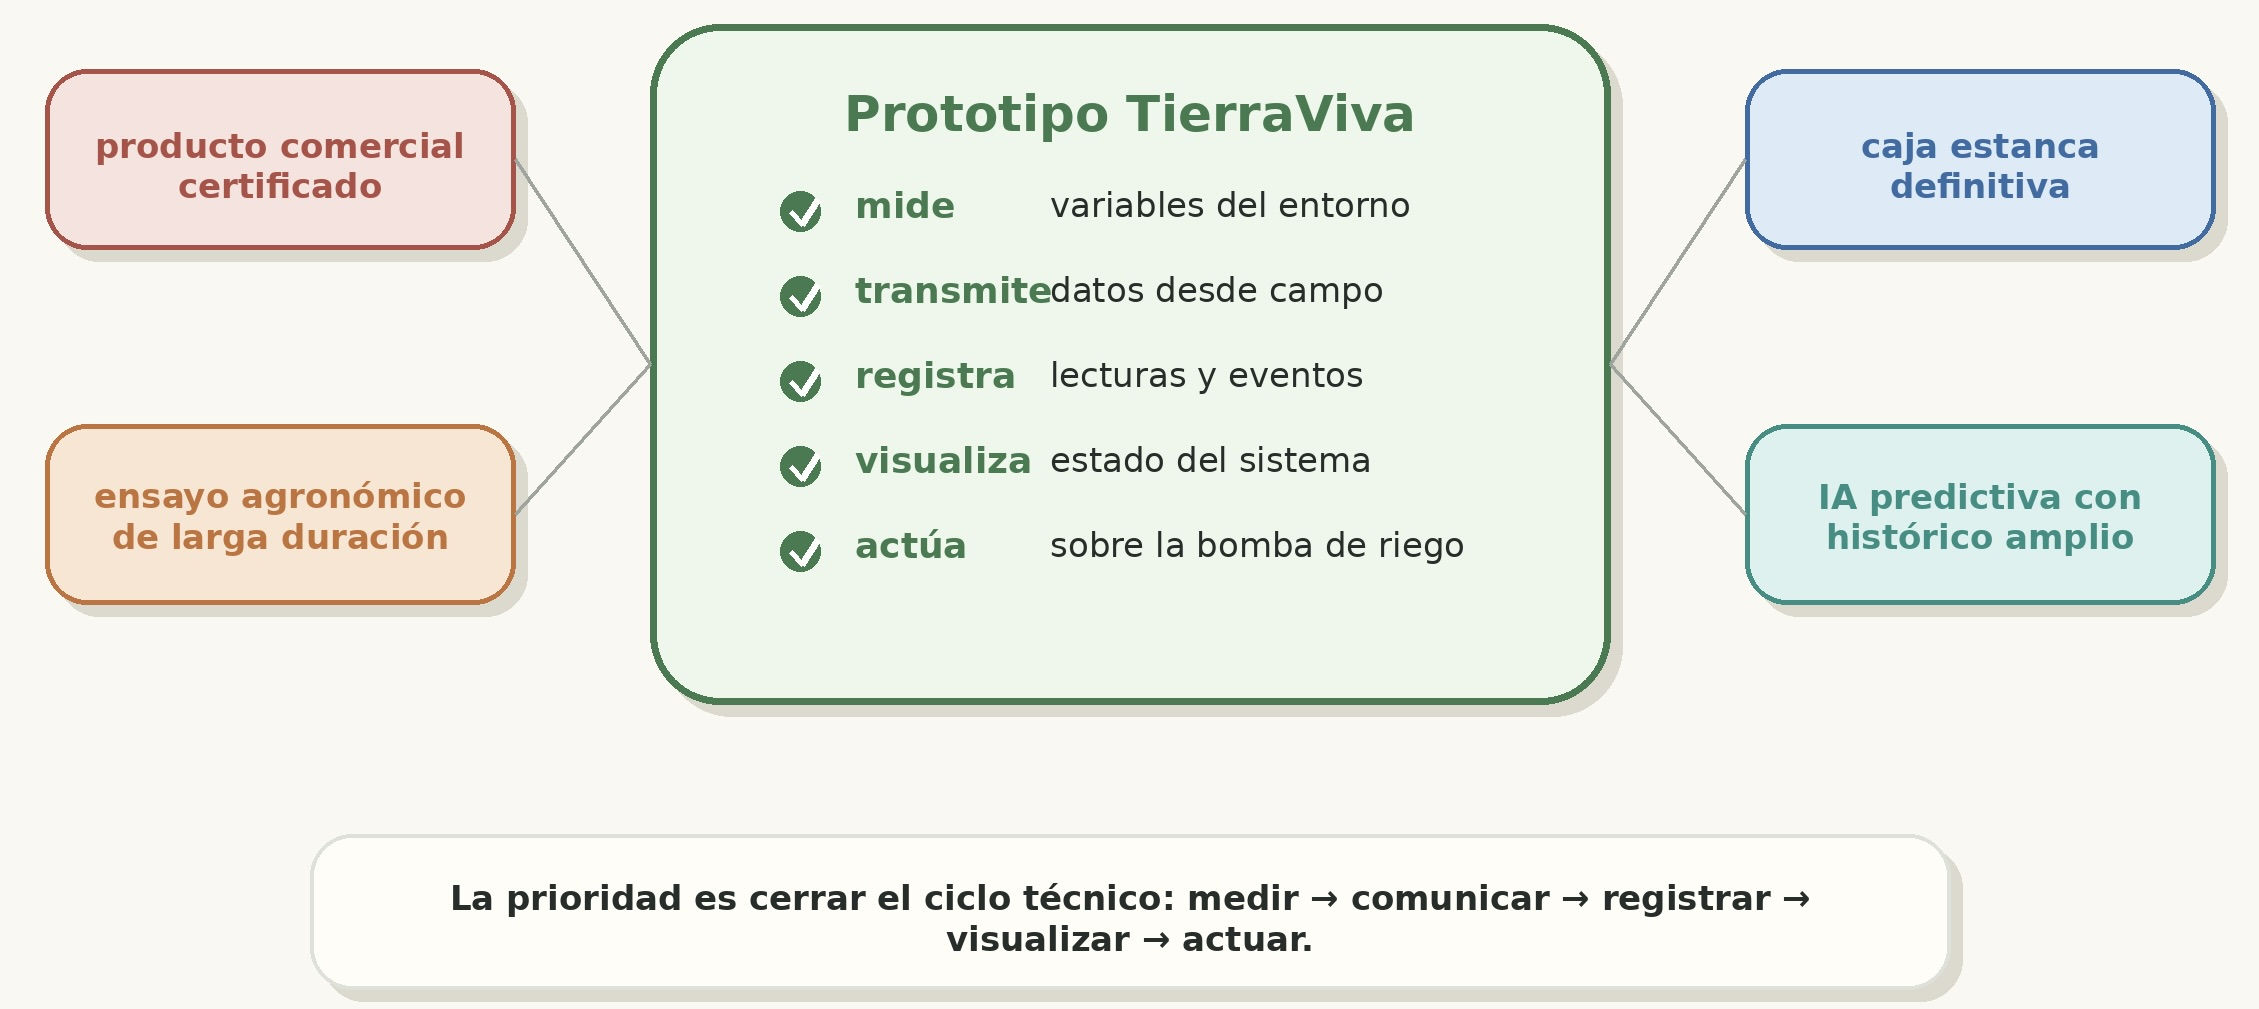
\includegraphics[width=0.96\textwidth]{figs/fig_cap1_05_alcance_prototipo.jpeg}
    \caption{Delimitación del alcance del prototipo TierraViva y de los aspectos que quedan fuera de esta fase del trabajo. Elaboración propia.}
    \label{fig:cap1_alcance_prototipo}
\end{figure}

No obstante, es importante delimitar claramente el alcance para evitar interpretar el proyecto como un sistema agrícola final preparado para su instalación directa en cualquier explotación. El prototipo desarrollado no pretende sustituir a soluciones profesionales de riego industrial, ni contempla certificaciones eléctricas, hidráulicas o de comunicaciones. Tampoco se aborda el diseño mecánico definitivo de una caja estanca, la fabricación de una placa electrónica propia ni la optimización completa del consumo energético para funcionamiento durante largos periodos sin mantenimiento.

Otra limitación relevante es la validación agronómica. Aunque el sistema está orientado al riego y se basa en variables relacionadas con el estado del entorno, no se realizará un ensayo prolongado durante varios meses sobre un cultivo real. Una validación de ese tipo requeriría controlar factores externos como el tipo de suelo, la especie cultivada, la climatología, la frecuencia de riego, la evolución del crecimiento de las plantas y la comparación con métodos tradicionales. En este TFG, la validación se centrará en comprobar que el prototipo mide, comunica, registra, visualiza y actúa correctamente, dejando los ensayos agronómicos de larga duración como una posible línea futura.

También se establece como limitación el uso de inteligencia artificial. Aunque el proyecto se plantea dentro de un contexto en el que la analítica de datos y los mecanismos predictivos pueden aportar mucho valor, no tendría rigor presentar como inteligencia artificial una lógica basada únicamente en reglas o umbrales. Para implementar modelos predictivos fiables sería necesario disponer de un histórico amplio de datos, recogido durante suficiente tiempo y bajo condiciones representativas. Por ello, en este trabajo la toma de decisiones se planteará de forma verificable mediante reglas, dejando la inteligencia artificial como una ampliación futura si se dispone de datos suficientes para entrenar, validar y justificar un modelo.

El sistema se diseñará con una visión modular, de modo que pueda ampliarse posteriormente con nuevas estaciones, nuevas variables medidas, mejoras en la autonomía energética o mecanismos más avanzados de análisis. Sin embargo, dentro del alcance de esta memoria, la prioridad será demostrar que la arquitectura propuesta funciona de extremo a extremo: desde la adquisición de datos en campo hasta la visualización y actuación sobre el riego. Esta delimitación permite mantener un equilibrio entre ambición y viabilidad, evitando prometer funcionalidades que no puedan ser implementadas y validadas con suficiente solidez durante el desarrollo del TFG.

Asimismo, en los capítulos finales de la memoria se incorporará una valoración del impacto social y ambiental del proyecto. Esta valoración analizará de qué forma TierraViva contribuye potencialmente a las metas ODS identificadas, especialmente en relación con agricultura sostenible, eficiencia en el uso del agua y gestión responsable de recursos. También se señalarán las limitaciones que impiden afirmar todavía un impacto cuantificado, así como posibles aspectos pendientes de mejora, como la optimización energética, la durabilidad del prototipo o la validación agronómica prolongada.

En resumen, el alcance del proyecto es el de un prototipo funcional, documentado y validado, orientado a demostrar la viabilidad técnica de un sistema IoT para riego inteligente. Sus limitaciones no se consideran una debilidad del trabajo, sino una forma de definir con precisión qué se ha implementado, qué se ha probado y qué queda abierto para futuras fases de desarrollo.

\section{Organización de la memoria}
\label{sec:organizacion_memoria}

La memoria se organiza de forma progresiva, comenzando por la introducción del problema y avanzando después hacia los fundamentos técnicos, las decisiones de diseño, la implementación y la validación del sistema.

En el Capítulo 1 se presenta el contexto del proyecto, la motivación, el planteamiento del problema y el alcance del trabajo. El Capítulo 2 recoge el estado del arte y los fundamentos tecnológicos necesarios para comprender la solución propuesta, incluyendo arquitecturas IoT, agricultura de precisión, comunicaciones, plataformas cloud y automatización del riego.

El Capítulo 3 describe los métodos, materiales y decisiones de diseño, definiendo los requisitos del sistema, la metodología seguida, la arquitectura general planteada y la justificación de las principales elecciones tecnológicas. A continuación, el Capítulo 4 presenta la arquitectura final de TierraViva y explica cómo se integran las estaciones de campo, la plataforma cloud, la Raspberry Pi como sistema de supervisión y los mecanismos locales de actuación.

Los Capítulos 5 y 6 se centran en la implementación del prototipo. El primero aborda la parte \textit{hardware} y \textit{firmware} de las estaciones, incluyendo la lectura de sensores, la publicación de telemetría y la decisión local de riego, mientras que el segundo describe la implementación software de supervisión en Raspberry Pi y nube. Posteriormente, el Capítulo 7 recoge la validación y las pruebas realizadas, desde la comprobación por bloques hasta la prueba funcional en Agrolab Móstoles.

Finalmente, el Capítulo 8 integra los resultados obtenidos, la discusión técnica de la solución, la valoración cualitativa recibida durante la prueba en Agrolab, las limitaciones detectadas, las líneas de trabajo futuro y las conclusiones finales del Trabajo de Fin de Grado.

\chapter{Estado del arte y fundamentos tecnológicos}
\label{cap:capitulo2}

Este capítulo recoge los fundamentos tecnológicos que sirven de base para el diseño de TierraViva. La revisión se centra en las áreas que han condicionado decisiones reales del proyecto: arquitecturas IoT, agricultura de precisión, redes de sensores, plataformas embebidas, conectividad en campo, protocolos de aplicación, plataformas cloud y automatización aplicada al riego.

El capítulo no busca valorar cada tecnología de forma aislada, sino explicar qué aporta cada una dentro de una arquitectura de riego inteligente. Por eso se presta atención tanto a sus ventajas como a sus restricciones prácticas: consumo, cobertura, facilidad de integración, dependencia de infraestructura y capacidad de validación dentro del alcance del TFG.

\section{Arquitectura funcional de sistemas IoT}
\label{sec:arquitecturas_iot}

El concepto de Internet de las Cosas (IoT, del inglés \textit{Internet of Things}) hace referencia a la interconexión de objetos físicos o virtuales capaces de identificarse, comunicarse y participar en servicios digitales. La recomendación del Sector de Normalización de las Telecomunicaciones de la Unión Internacional de Telecomunicaciones (ITU-T, del inglés \textit{International Telecommunication Union -- Telecommunication Standardization Sector}) Y.2060 define IoT como una infraestructura global para la sociedad de la información que permite ofrecer servicios avanzados mediante la interconexión de cosas físicas y virtuales a través de tecnologías interoperables \cite{itu_y2060}. Esta definición resulta adecuada para TierraViva porque sitúa IoT como una arquitectura completa: adquisición de datos, comunicación, procesamiento, almacenamiento, visualización y, cuando procede, actuación física.

Desde un punto de vista práctico, un sistema IoT conecta el mundo físico con el mundo digital. En el extremo de campo se encuentran dispositivos capaces de medir variables, detectar eventos o modificar el estado de un sistema. Esa información se transmite hacia otras capas, donde puede almacenarse, procesarse, visualizarse o utilizarse para apoyar decisiones. Cuando el sistema incorpora control, la actuación puede resolverse mediante lógica centralizada, control remoto o decisión local en el propio nodo. Esta última alternativa es especialmente relevante cuando se desea que el sistema conserve un comportamiento seguro aunque la conectividad externa no esté disponible.

\begin{figure}[H]
    \centering
    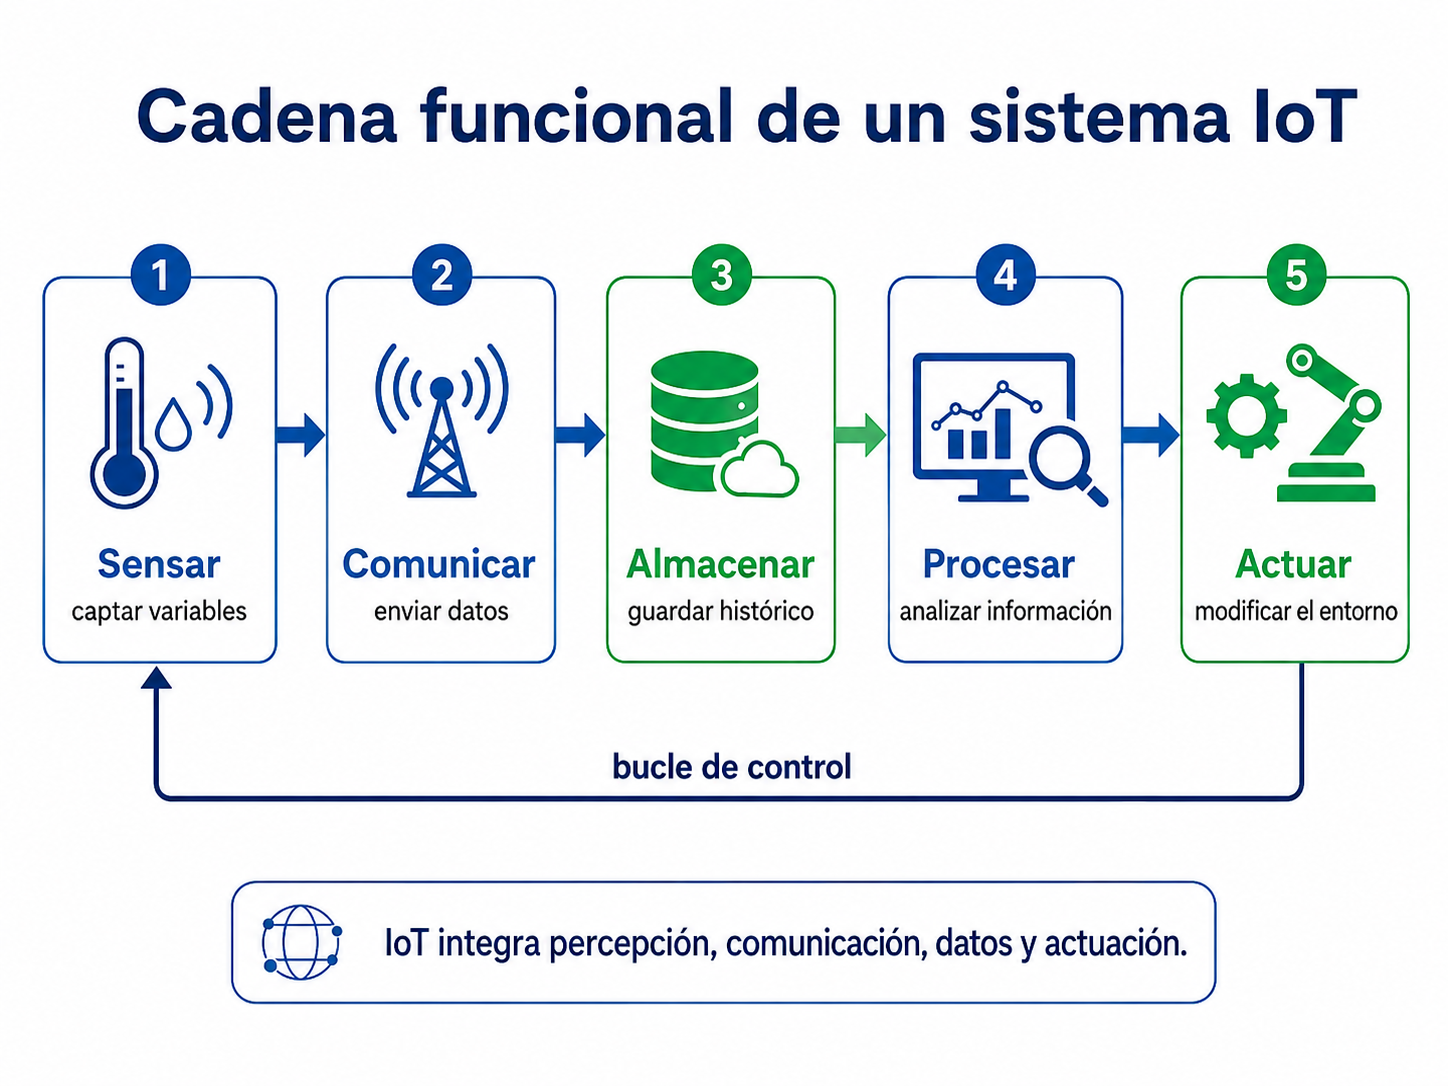
\includegraphics[width=0.95\textwidth]{figs/figura_2_1_cadena_funcional_iot.png}
    \caption{Cadena funcional básica de un sistema IoT. El sistema capta información del entorno mediante sensorización, la transmite a través de una red, la almacena, la procesa y, cuando procede, actúa sobre el mundo físico cerrando el bucle de control. Elaboración propia, véase Anexo~\ref{sec:uso_ia_generativa_tfg}.}
    \label{fig:cap2_cadena_funcional_iot}
\end{figure}

En una arquitectura IoT no basta con que cada componente funcione de forma aislada. Sensores, actuadores, plataformas embebidas, redes de comunicación, servicios de datos, bases de datos, API y \textit{dashboards} deben integrarse de forma coherente. Un sistema puede fallar aunque sus sensores sean correctos si la comunicación, la persistencia o la lógica de actuación no están bien definidas.

Uno de los elementos básicos es el nodo terminal o \textit{end-device}, situado cerca del fenómeno que se quiere observar o controlar. Normalmente integra sensores, unidad de procesamiento, sistema de comunicación y fuente de alimentación. Estos nodos suelen estar limitados en memoria, capacidad de cálculo, consumo energético o ancho de banda, por lo que sus restricciones deben considerarse desde el diseño inicial \cite{alFuqaha2015iot}. Cuando además incorporan actuadores, el diseño debe diferenciar claramente entre monitorización y control, ya que una decisión incorrecta puede tener consecuencias físicas.

En muchas arquitecturas aparece una pasarela o \textit{gateway}, encargada de agregar datos, traducir protocolos, filtrar información o proporcionar salida hacia redes de mayor alcance. Este enfoque se relaciona con la computación en el borde o \textit{edge computing}, que desplaza parte del procesamiento hacia elementos próximos al fenómeno físico \cite{ieee2413_2019}. En sistemas con actuación, esta idea permite aplicar reglas de seguridad cerca del dispositivo de campo y reducir la dependencia de servicios externos.

La nube o plataforma \textit{cloud} aporta almacenamiento, disponibilidad remota, interfaces programables y herramientas de visualización. Sin embargo, también introduce dependencias de conectividad, latencia, disponibilidad del servicio y límites de uso. Por ello, en sistemas con actuación física resulta conveniente decidir qué parte del comportamiento debe ejecutarse localmente y qué parte puede delegarse en capas remotas.

Las arquitecturas IoT suelen representarse por capas. Una división sencilla distingue entre capa física, conectividad, procesamiento y almacenamiento, y aplicación. Modelos más completos, como el propuesto por el IoT World Forum, añaden niveles como computación en el borde, acumulación de datos, abstracción y procesos de negocio \cite{hanes2017iot}.

\begin{figure}[H]
    \centering
    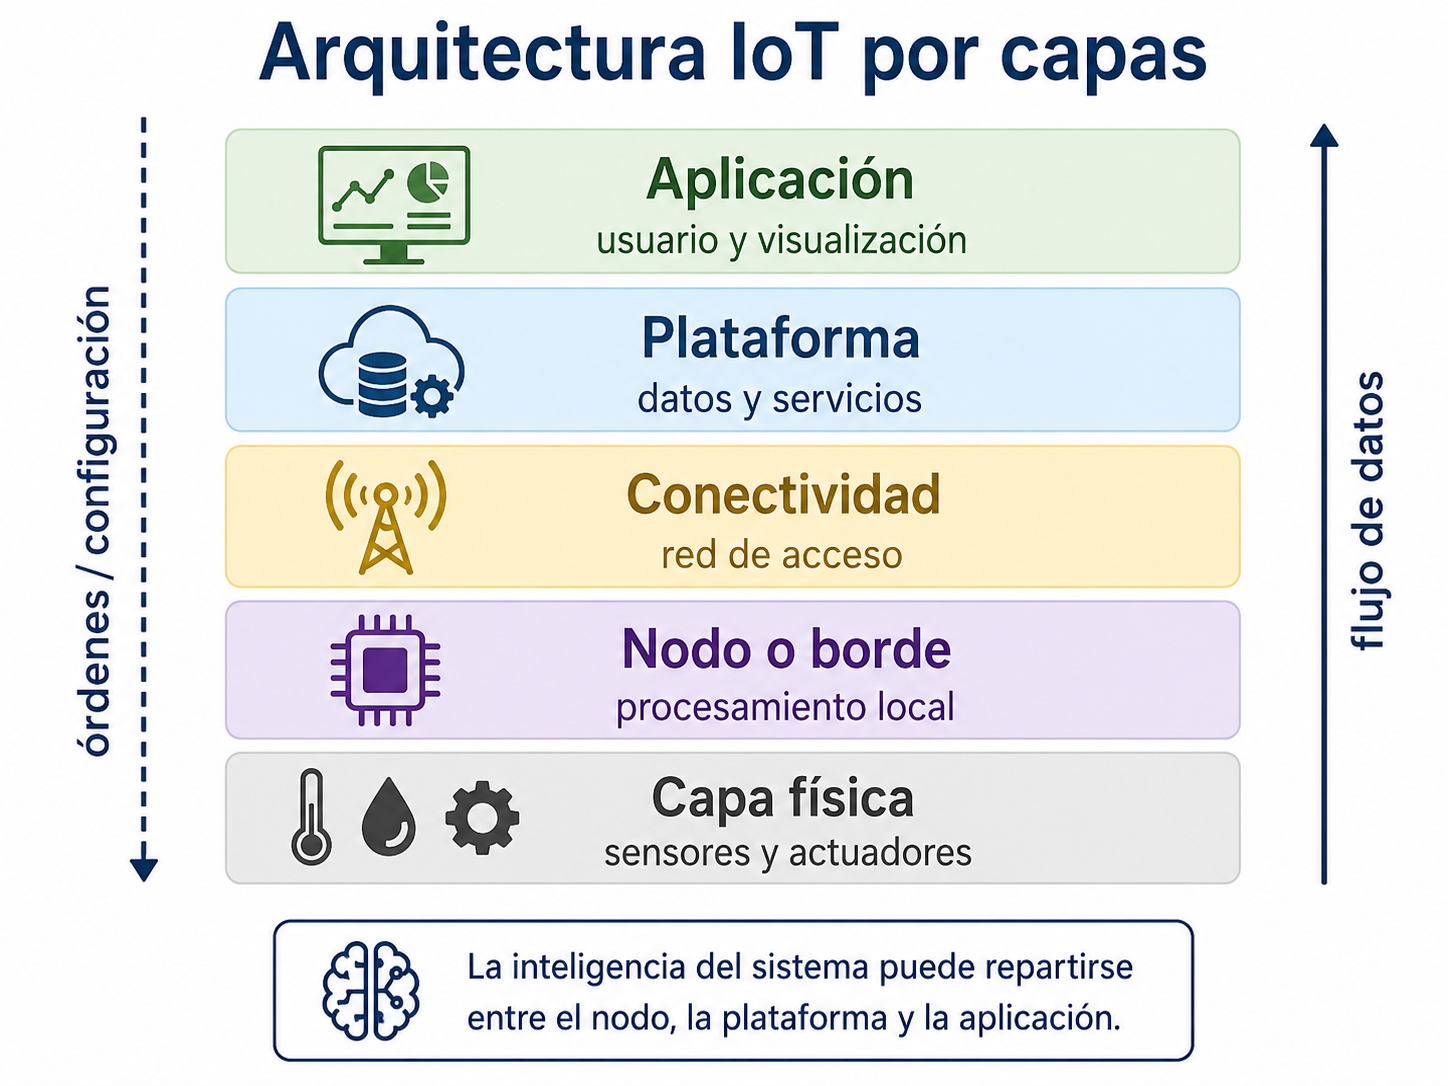
\includegraphics[width=0.75\textwidth]{figs/figura_2_2_arquitectura_iot_capas.png}
    \caption{Arquitectura IoT organizada por capas funcionales. Elaboración propia, véase Anexo~\ref{sec:uso_ia_generativa_tfg}.}
    \label{fig:cap2_arquitectura_iot_capas}
\end{figure}

La Figura~\ref{fig:cap2_arquitectura_iot_capas} resume esta estructura. En TierraViva, esta organización se traduce en estaciones de campo que miden y actúan localmente, una plataforma intermedia para telemetría, una Raspberry Pi para ingesta y supervisión local, una base de datos, una API y un \textit{dashboard}. La actuación de riego no depende de una orden remota, sino de la lógica local de la estación.

\section{Agricultura de precisión y riego inteligente}
\label{sec:agricultura_precision_riego}

La agricultura de precisión es una estrategia de gestión agrícola que utiliza datos para tomar decisiones más ajustadas a las condiciones reales de cada explotación, parcela o zona de cultivo. Según la International Society of Precision Agriculture, este enfoque se basa en recopilar, procesar y analizar datos temporales, espaciales e individuales, combinándolos con otra información para apoyar decisiones de manejo orientadas a mejorar la eficiencia en el uso de recursos, la productividad, la calidad, la rentabilidad y la sostenibilidad de la producción agrícola \cite{ispa_precision_agriculture_definition}.

El interés de este enfoque está en la variabilidad del entorno agrícola. Una misma parcela puede presentar diferencias de humedad, exposición solar, tipo de suelo, pendiente o desarrollo de las plantas. Si todas las zonas se tratan de la misma manera, parte de esa variabilidad queda oculta. La agricultura de precisión intenta reducir esa simplificación utilizando datos para adaptar mejor las decisiones.

El agua es una variable crítica dentro de este contexto. La agricultura representa una parte muy relevante de las extracciones de agua dulce a escala global; AQUASTAT indica que aproximadamente el 69\% de las extracciones corresponden al uso agrícola \cite{fao_aquastat_water_use}. Una mejora en la gestión del riego puede afectar tanto al rendimiento del cultivo como a la sostenibilidad del recurso. Regar de forma inadecuada puede provocar déficit hídrico, exceso de agua, pérdida de eficiencia y deterioro del cultivo.

El riego manual depende de la presencia y experiencia del usuario. Puede funcionar en cultivos pequeños o con supervisión frecuente, pero presenta limitaciones cuando el terreno no puede revisarse de forma continua. El riego temporizado reduce la intervención manual programando horarios o duraciones concretas, aunque sigue siendo rígido: puede mantener el mismo patrón aunque cambien la temperatura, la humedad, la lluvia o la exposición solar.

El riego basado en datos introduce una lógica diferente. La decisión de regar se apoya en medidas del entorno, como humedad del suelo, temperatura ambiente, humedad relativa, radiación o luminosidad, previsión meteorológica, tipo de cultivo o histórico de riego. No todas las variables tienen el mismo peso, pero su combinación permite interpretar mejor el estado del sistema agrícola.

La monitorización ambiental permite pasar de una decisión basada en intuición a una decisión basada en información observable. Además, el registro de datos a lo largo del tiempo permite estudiar tendencias, detectar cambios bruscos y comprobar si una acción de riego ha tenido el efecto esperado.

Cuando la monitorización se conecta con un mecanismo de actuación, el sistema pasa a formar parte del control del proceso. En ese punto aparecen requisitos adicionales: reglas claras, límites de seguridad y comportamiento seguro ante fallo. En riego, una actuación incorrecta puede traducirse en pérdida de agua, daño al cultivo o funcionamiento indebido del actuador encargado de impulsar o permitir el paso del agua.

Los sistemas de riego inteligente basados en IoT suelen combinar nodos de medida, comunicaciones, almacenamiento de datos, procesamiento y actuación. Por ejemplo, Boursianis et al. presentan en \textit{IEEE Sensors Journal}, revista del \textit{Institute of Electrical and Electronics Engineers} (IEEE), una plataforma de riego inteligente para agricultura de precisión basada en IoT, planteada como un sistema formado por varios subsistemas coordinados \cite{boursianis2021smart_irrigation}. Esta línea de trabajo es relevante porque desplaza el foco desde el sensor aislado hacia la arquitectura completa.

En TierraViva este enfoque se concreta en una decisión sencilla pero importante: no basta con medir humedad o temperatura, la estación debe convertir esas lecturas en una actuación local limitada y segura. La literatura sobre agricultura inteligente resalta que el valor de IoT no está únicamente en instalar sensores, sino en integrar monitorización, comunicación, procesamiento, almacenamiento, supervisión y toma de decisiones dentro de una arquitectura fiable \cite{shafi2019,soussi2024smart,abioye2020}. Por ello, la eficiencia del sistema depende tanto de la calidad de las medidas como de la forma en que una lectura se transforma en una acción de riego controlada.

\section{Redes de sensores y nodos de campo}
\label{sec:redes_sensores_nodos_campo}

Una red de sensores es un conjunto de dispositivos distribuidos que capturan información del entorno y la transmiten hacia un sistema capaz de procesarla, almacenarla o utilizarla para tomar decisiones. En IoT, estas redes permiten observar fenómenos físicos de forma continua y en distintos puntos del espacio.

El elemento básico es el nodo de campo o \textit{end-node}. Se sitúa cerca del entorno que se quiere medir o controlar y normalmente incorpora una unidad de procesamiento, uno o varios sensores, un sistema de comunicación y una fuente de alimentación \cite{hanes2017iot}. En agricultura, estos nodos pueden instalarse en distintas zonas de cultivo para recoger datos periódicos y enviarlos a un sistema de supervisión.

Dentro de una red conviene distinguir entre nodos sensores y nodos actuadores. Un nodo actuador modifica físicamente el estado de un sistema, por ejemplo activando una bomba, cerrando un circuito mediante un relé o accionando otro elemento físico de riego. En muchos sistemas reales ambas funciones conviven en un mismo nodo.

Los sensores transforman una magnitud física en una señal interpretable por el sistema. En agricultura son habituales variables como humedad del suelo, temperatura ambiente, humedad relativa, luminosidad, presión atmosférica, radiación solar, caudal o parámetros químicos del suelo. En riego, las variables relacionadas con el agua disponible y las condiciones ambientales tienen prioridad \cite{garcia2020}.

Una diferencia importante es el tipo de salida del sensor. Los sensores analógicos generan una señal continua, normalmente una tensión o corriente proporcional a la magnitud medida, y requieren conversión analógico-digital. Los sensores digitales entregan directamente la medida mediante un protocolo de comunicación. Los primeros suelen ser sencillos y económicos, pero más sensibles al ruido y a la alimentación; los segundos facilitan la lectura, aunque dependen de protocolos, direcciones y librerías concretas.

\begin{table}[H]
\begin{center}
\renewcommand{\arraystretch}{1.15}
\rowcolors{2}{TableRowSoft}{white}

\begin{tabular}{|p{0.24\textwidth}|p{0.32\textwidth}|p{0.32\textwidth}|}
\hline
\rowcolor{URJCRed}
\TVHead{Aspecto} & \TVHead{Sensores analógicos} & \TVHead{Sensores digitales} \\
\hline
Salida & Señal continua proporcional a la magnitud medida. & Dato digital entregado por un bus o protocolo. \\
\hline
Lectura & Requieren conversión analógico-digital. & Se leen mediante comunicación digital. \\
\hline
Ventajas & Simples, económicos y fáciles de conectar. & Lectura más directa y mayor integración interna. \\
\hline
Limitaciones & Sensibles a ruido, alimentación y cableado. & Dependencia de protocolos, direcciones y librerías. \\
\hline
Uso habitual & Medidas sencillas con salida proporcional. & Sensores con varias magnitudes o calibración interna. \\
\hline
\end{tabular}
\caption{Comparación general entre sensores analógicos y digitales}
\label{cuadro:sensores_analogicos_digitales}
\end{center}
\end{table}

La Tabla~\ref{cuadro:sensores_analogicos_digitales} recoge esta comparación. En ambos casos, una lectura de sensor no debe asumirse como una medida absoluta. Muchos sensores necesitan calibración para que sus valores sean útiles en un contexto concreto. En agricultura esto es evidente en variables como la humedad del suelo, cuya respuesta puede depender del sustrato, la compactación, la salinidad, la temperatura o la forma de instalación.

También deben contemplarse errores de medida. Un sensor puede devolver valores erróneos por ruido eléctrico, mala conexión, humedad, degradación, fallos de alimentación o condiciones fuera de rango. Si esas medidas se utilizan para tomar decisiones automáticas, el sistema debe diferenciar entre datos válidos, datos dudosos y ausencia de datos. Esta distinción evita que una actuación dependa de una única lectura incoherente.

Los nodos de campo suelen tener recursos limitados. Pueden funcionar con batería, comunicarse mediante enlaces de bajo ancho de banda y operar en zonas de cobertura irregular. El diseño debe decidir qué datos se envían, con qué frecuencia, a qué distancia y cuántos nodos formarán parte de la red \cite{alFuqaha2015iot}.

\begin{figure}[H]
    \centering
    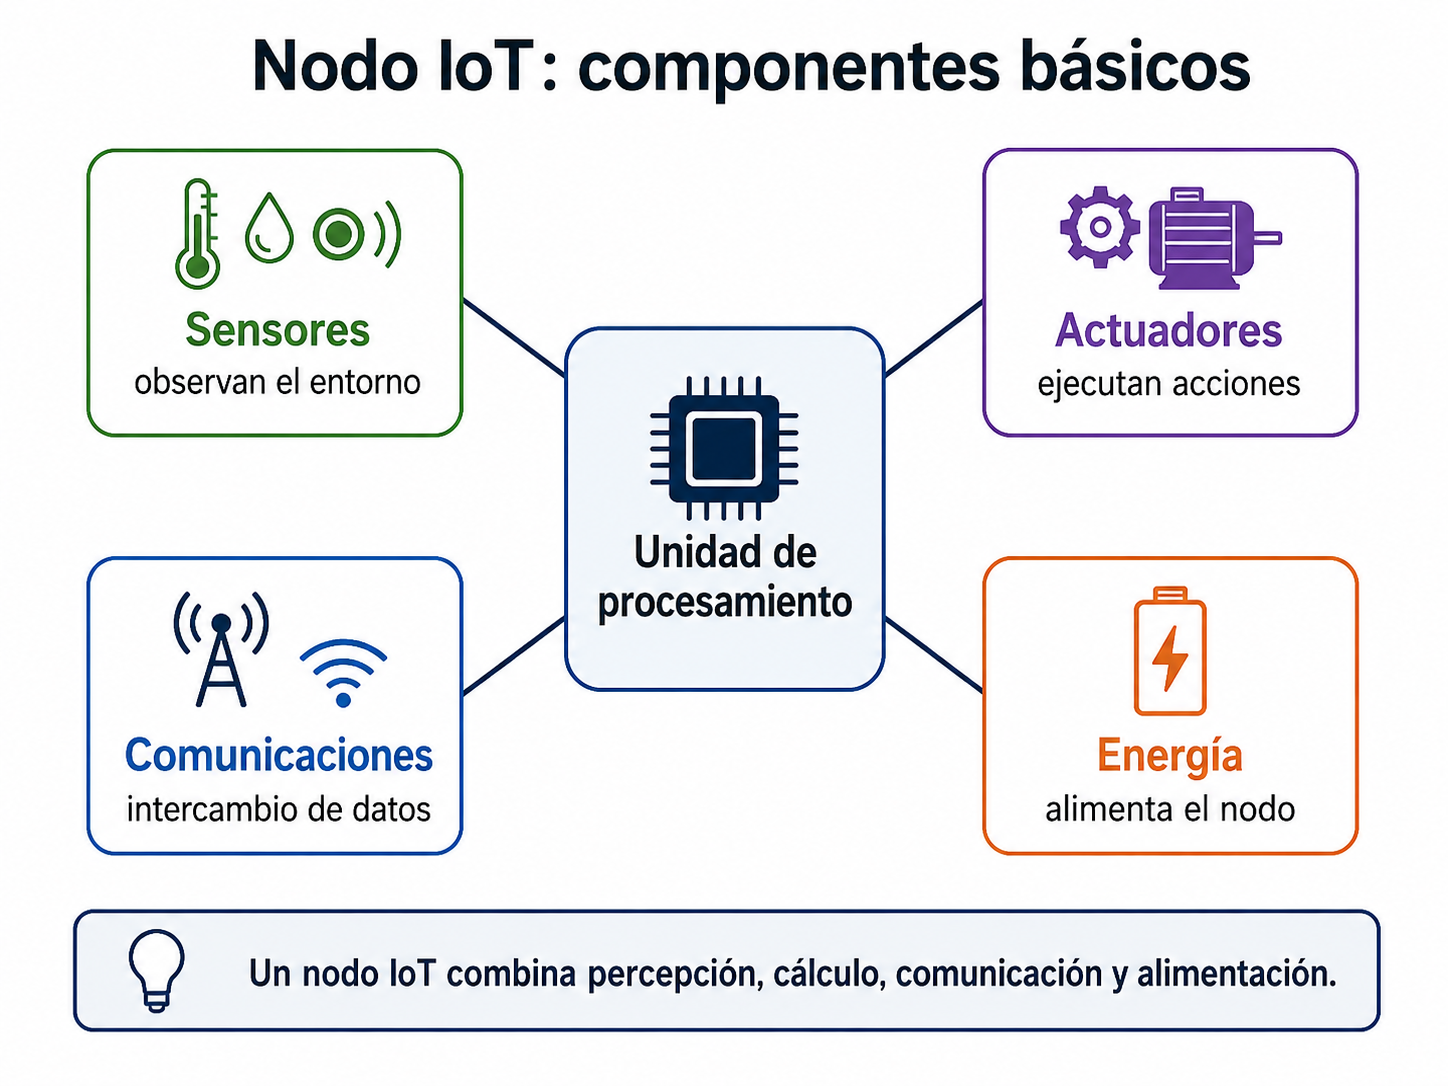
\includegraphics[width=0.92\textwidth]{figs/figura_2_3_nodo_iot_componentes.png}
    \caption{Componentes básicos de un nodo IoT. Un nodo integra sensores para observar el entorno, actuadores para ejecutar acciones, una unidad de procesamiento, un subsistema de comunicaciones y una fuente de energía que condiciona su autonomía. Elaboración propia, véase Anexo~\ref{sec:uso_ia_generativa_tfg}.}
    \label{fig:cap2_nodo_iot_componentes}
\end{figure}

La Figura~\ref{fig:cap2_nodo_iot_componentes} muestra los bloques habituales de un nodo de campo. En una aplicación agrícola real, la fiabilidad depende del conjunto formado por sensor, nodo, alimentación, comunicación, protección física y tratamiento de datos \cite{soussi2024smart}. Cuando el nodo incorpora un actuador, también debe asumir reglas mínimas de actuación segura, ya que es el elemento que se encuentra físicamente conectado al sistema de riego.

\section{Arquitectura de red IoT}
\label{sec:arquitectura_red_iot}

Antes de comparar plataformas hardware concretas, conviene distinguir los elementos funcionales que forman una arquitectura de red IoT. Esta separación evita confundir el papel que cumple un elemento dentro del sistema con el tipo de dispositivo físico utilizado para implementarlo. Por ejemplo, un nodo de campo puede estar implementado con un microcontrolador, pero el concepto de nodo no equivale al concepto de microcontrolador; del mismo modo, una pasarela puede ejecutarse en un computador de placa única, en un router industrial o en otro dispositivo con capacidad de comunicación y procesamiento.

De forma general, una arquitectura de red IoT se organiza alrededor de varios elementos funcionales. En el extremo físico se encuentran los nodos terminales o nodos de campo, que capturan información del entorno y, en algunos casos, actúan sobre él. Estos nodos se conectan mediante una red de acceso, que puede basarse en tecnologías de corto alcance, redes de área extensa y bajo consumo, conectividad celular u otras soluciones inalámbricas o cableadas. Entre los nodos y los servicios de datos puede existir una pasarela o \textit{gateway}, encargada de agregar información, traducir protocolos, filtrar datos o proporcionar salida hacia Internet. Finalmente, la plataforma de datos, el backend y las aplicaciones de usuario permiten almacenar, procesar, consultar y visualizar la información.

La Tabla~\ref{tab:arquitectura_red_iot_elementos} resume estos elementos desde un punto de vista funcional. Entre las tecnologías que pueden formar parte de una red de acceso se encuentran WiFi, LoRa, LoRaWAN (\textit{Long Range Wide Area Network}), LTE (\textit{Long Term Evolution}), NB-IoT (\textit{Narrowband Internet of Things}) o Ethernet, entre otras. Las diferencias entre estas opciones se desarrollan posteriormente en el apartado dedicado a conectividad en entornos rurales.

\begin{table}[H]
\begin{center}
\small
\renewcommand{\arraystretch}{1.15}
\rowcolors{2}{TableRowSoft}{white}
\begin{tabular}{|p{0.24\textwidth}|p{0.42\textwidth}|p{0.24\textwidth}|}
\hline
\rowcolor{URJCRed}
\TVHead{Elemento funcional} & \TVHead{Responsabilidad dentro de la arquitectura} & \TVHead{Ejemplos de implementación} \\
\hline
Nodo terminal o nodo de campo & Mide variables físicas, genera telemetría y, si incorpora actuadores, puede ejecutar acciones locales. & Arduino, ESP32, STM32, módulos embebidos específicos. \\
\hline
Red de acceso & Proporciona conectividad entre los nodos de campo y el resto del sistema. & WiFi, LoRa/LoRaWAN, LTE, NB-IoT, Ethernet. \\
\hline
Pasarela o \textit{gateway} & Agrega datos, traduce protocolos, ejecuta procesamiento local o proporciona salida hacia redes externas. & Router, gateway LoRaWAN, Raspberry Pi, equipo embebido industrial. \\
\hline
Plataforma de datos & Recibe, almacena y hace accesible la telemetría publicada por los dispositivos. & ThingSpeak, ThingsBoard, \textit{broker} de mensajería, plataforma cloud propia. \\
\hline
Backend o sistema de supervisión & Valida, transforma, almacena y expone los datos mediante servicios o interfaces programables. & Servidor local, Raspberry Pi, servicio cloud. \\
\hline
Aplicación de usuario & Permite consultar el estado del sistema, revisar históricos, visualizar alertas o analizar tendencias. & Dashboard web, aplicación móvil, panel cloud. \\
\hline
\end{tabular}
\caption{Elementos funcionales habituales en una arquitectura de red IoT.}
\label{tab:arquitectura_red_iot_elementos}
\end{center}
\end{table}

Esta distinción permite analizar posteriormente qué plataforma resulta más adecuada para cada función. La arquitectura define primero qué elementos son necesarios y cómo se relacionan entre sí; después se decide con qué tecnología se implementa cada elemento. En sistemas agrícolas, esta separación es especialmente importante porque los nodos de campo suelen estar condicionados por consumo, conectividad, protección ambiental y autonomía, mientras que los sistemas de supervisión pueden requerir más capacidad de almacenamiento, servicios software e interfaces de consulta.

En una arquitectura IoT con riego automático también debe diferenciarse entre flujo ascendente y flujo descendente. El flujo ascendente transporta medidas, estados y eventos desde los nodos de campo hacia la plataforma o sistema de supervisión. El flujo descendente, cuando existe, transporta órdenes, configuraciones o consignas hacia los dispositivos de campo. En sistemas con actuación física, el diseño debe decidir si la orden de actuación depende de una capa remota o si se ejecuta localmente en el nodo. Esta decisión afecta directamente a la seguridad, latencia y tolerancia a fallos del sistema. Esta distinción entre elemento funcional y tecnología de implementación se utilizará en el apartado siguiente para comparar microcontroladores y computadores de placa única sin confundirlos con los roles arquitectónicos que pueden desempeñar.

\section{Controladores y plataformas embebidas para IoT}
\label{sec:controladores_plataformas_embebidas}

Una vez definidos los elementos funcionales de una arquitectura de red IoT, puede analizarse qué tipo de plataforma de cómputo resulta adecuada para implementar cada uno de ellos. Esta decisión pertenece al nivel de implementación: no define por sí misma la arquitectura, sino la tecnología concreta con la que se materializan sus bloques.

En este contexto conviene diferenciar entre microcontroladores y computadores de placa única, también denominados \textit{single-board computers} (SBC) o sistemas en placa. Los primeros suelen emplearse en nodos terminales por su bajo consumo, arranque inmediato y facilidad para interactuar con sensores y actuadores. Los segundos ofrecen más capacidad software y pueden ejecutar sistemas operativos completos, por lo que resultan adecuados para funciones de pasarela, backend local, almacenamiento, interfaces programables o visualización.

Los microcontroladores son una opción habitual para nodos de campo. Son dispositivos de bajo coste y consumo reducido, pensados para ejecutar tareas concretas de forma repetitiva: leer sensores, activar salidas digitales, comunicarse mediante buses sencillos o enviar datos a través de un módulo externo. Plataformas como Arduino, ESP32, STM32 u otras equivalentes son frecuentes en prototipos IoT porque permiten trabajar directamente con entradas y salidas físicas, temporización, comunicaciones serie y buses como I2C (\textit{Inter-Integrated Circuit}) o SPI (\textit{Serial Peripheral Interface}) \cite{alFuqaha2015iot}.

Arduino es una familia muy extendida en educación y prototipado. Su principal ventaja es el entorno accesible, la abundante documentación y la compatibilidad con muchos sensores y módulos. ESP32 incorpora WiFi y Bluetooth, además de mayor potencia de cálculo. Las familias STM32 ofrecen más control técnico y una gama amplia de prestaciones, aunque suelen exigir mayor conocimiento del entorno de desarrollo y de la configuración de periféricos.

Los computadores de placa única o SBC, como Raspberry Pi u otras plataformas similares, cubren otro tipo de necesidades. Permiten ejecutar un sistema operativo completo, levantar servicios, gestionar bases de datos, servir aplicaciones web o coordinar varios procesos software. Su mayor potencia y flexibilidad los hace adecuados para almacenamiento, visualización, supervisión, análisis histórico o funciones de gateway. A cambio, consumen más, arrancan más lentamente y no son la opción natural para depender de ellos como único punto de decisión en una actuación física crítica.

La diferencia entre ambas familias no debe interpretarse como una equivalencia directa entre tecnología y elemento arquitectónico. Un microcontrolador no es una arquitectura, sino una forma habitual de implementar un nodo terminal sencillo. Del mismo modo, un computador de placa única no es necesariamente una pasarela, aunque puede desempeñar ese papel si se configura para agregar datos, ejecutar servicios o comunicar redes distintas. La elección depende de la función que deba cubrirse, del consumo admisible, de las interfaces necesarias y de la complejidad software requerida.

En la comparativa se emplean además varias siglas habituales en plataformas embebidas: GPIO (\textit{General Purpose Input/Output}) para pines de entrada y salida digital, ADC (\textit{Analog-to-Digital Converter}) para conversión analógico-digital, PWM (\textit{Pulse Width Modulation}) para modulación por ancho de pulso, UART (\textit{Universal Asynchronous Receiver-Transmitter}) para comunicación serie y USB (\textit{Universal Serial Bus}) para conexión de periféricos o programación.

\begin{table}[H]
\begin{center}
\small
\renewcommand{\arraystretch}{1.15}
\rowcolors{2}{TableRowSoft}{white}
\begin{tabular}{|p{0.24\textwidth}|p{0.32\textwidth}|p{0.32\textwidth}|}
\hline
\rowcolor{URJCRed}
\TVHead{Aspecto} & \TVHead{Microcontroladores} & \TVHead{Computadores de placa única o SBC} \\
\hline
Naturaleza & Circuitos integrados o placas basadas en microcontrolador, orientadas a tareas embebidas concretas. & Placas completas capaces de ejecutar un sistema operativo y varios procesos software. \\
\hline
Uso habitual en IoT & Implementación de nodos terminales, lectura de sensores, control de salidas y lógica local sencilla. & Implementación de pasarelas, servidores locales, sistemas de supervisión, almacenamiento o visualización. \\
\hline
Consumo & Bajo o moderado, adecuado para dispositivos alimentados por batería si el diseño lo permite. & Superior, debido al sistema operativo, periféricos y servicios en ejecución. \\
\hline
Capacidad de cálculo & Suficiente para adquisición, temporización, comunicación básica y reglas simples. & Adecuada para bases de datos, interfaces programables, interfaces web, procesamiento histórico y coordinación de servicios. \\
\hline
Interfaces típicas & GPIO, ADC, PWM, UART, I2C, SPI y entradas/salidas cercanas al hardware. & GPIO, USB, Ethernet/WiFi, almacenamiento local, sistema operativo y servicios de red. \\
\hline
Limitaciones & Memoria reducida, menor capacidad de procesamiento y dificultad para ejecutar servicios complejos. & Mayor consumo, arranque más lento y dependencia de sistema operativo. \\
\hline
\end{tabular}
\caption{Comparación general entre microcontroladores y computadores de placa única como plataformas de implementación en IoT}
\label{cuadro:microcontroladores_sbc}
\end{center}
\end{table}

La Tabla~\ref{cuadro:microcontroladores_sbc} resume las diferencias entre ambas plataformas como opciones de implementación. En un sistema IoT agrícola, una arquitectura híbrida puede combinar nodos terminales implementados con microcontroladores y sistemas de supervisión implementados con computadores de placa única. Lo importante no es asociar rígidamente una tecnología a un elemento arquitectónico, sino asignar cada función al dispositivo que mejor responda a sus restricciones de consumo, interfaces, robustez y capacidad software \cite{hanes2017iot,soussi2024smart}.

\section{Comunicaciones de bajo consumo y conectividad en entornos rurales}
\label{sec:comunicaciones_lpwan}

La conectividad condiciona la viabilidad de cualquier sistema IoT desplegado en campo. En aplicaciones agrícolas, los nodos pueden estar separados de la vivienda, del laboratorio o del sistema de supervisión, y no siempre existe una infraestructura de red disponible. No se puede asumir WiFi estable, alimentación cercana ni cobertura móvil suficiente en todos los puntos.

El tráfico típico de estos sistemas suele ser reducido: humedad, temperatura, estado de un actuador, tensión de batería o avisos de error enviados cada cierto intervalo. La prioridad no es el caudal, sino la cobertura, el consumo, la disponibilidad y la fiabilidad del enlace.

\begin{figure}[H]
    \centering
    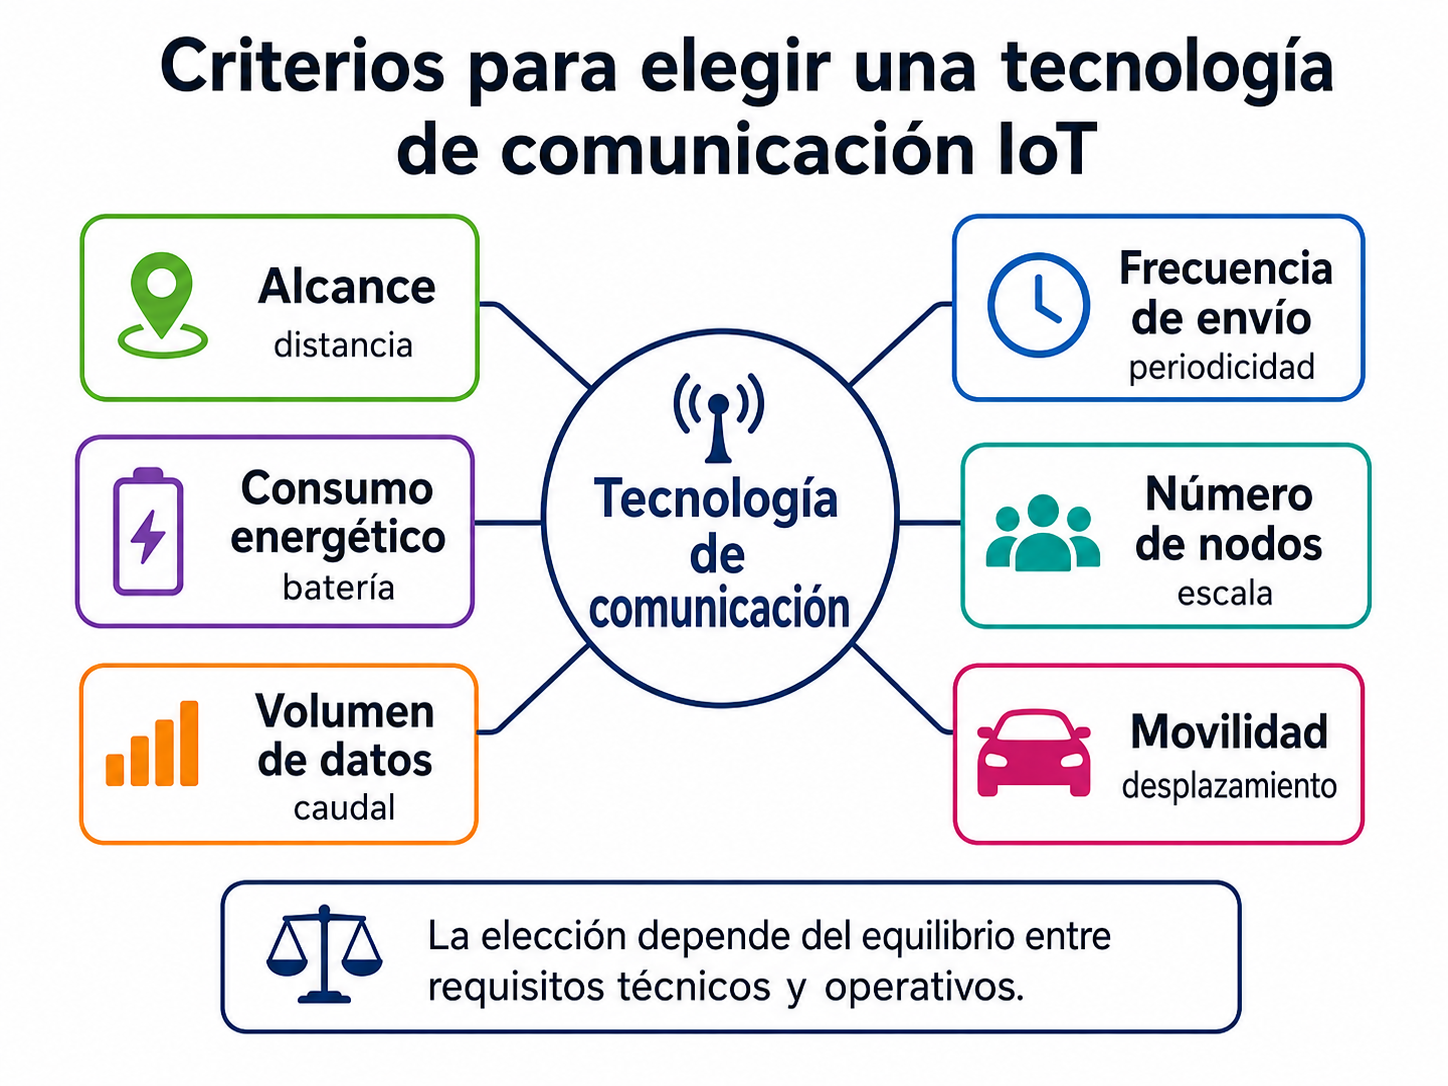
\includegraphics[width=\textwidth]{figs/figura_2_5_criterios_comunicacion_iot.png}
    \caption{Criterios principales para seleccionar una tecnología de comunicación en un sistema IoT. La elección depende del equilibrio entre alcance, consumo energético, volumen de datos, frecuencia de envío, número de nodos y movilidad del escenario de aplicación. Elaboración propia, véase Anexo~\ref{sec:uso_ia_generativa_tfg}.}
    \label{fig:cap2_criterios_comunicacion_iot}
\end{figure}

Las redes de área extensa y bajo consumo (LPWAN, del inglés \textit{Low-Power Wide-Area Networks}) se diseñan para dispositivos distribuidos que envían pequeñas cantidades de datos a largas distancias. A cambio, aceptan bajo caudal, mayor latencia o mensajes poco frecuentes \cite{raza2017lpwan}. Este compromiso encaja con muchas aplicaciones agrícolas, donde las variables ambientales no requieren actualización continua a escala de milisegundos.

WiFi y Bluetooth son tecnologías conocidas, pero su utilidad en campo abierto es limitada. WiFi ofrece alta capacidad, aunque depende de una red local cercana. Bluetooth, y especialmente BLE (\textit{Bluetooth Low Energy}), puede ser útil para configuración próxima o interacción local, pero no resuelve por sí solo estaciones separadas por grandes distancias.

Entre las tecnologías de largo alcance destacan LoRa, LoRaWAN y las redes celulares. LoRa hace referencia a una modulación radio de largo alcance y bajo consumo desarrollada por Semtech, mientras que LoRaWAN (\textit{Long Range Wide Area Network}) define una arquitectura de red completa formada por dispositivos finales, pasarelas y servidores de red \cite{semtech2015lora_modulation,augustin2016lora,lora_alliance_104}. Esta diferencia es importante: utilizar LoRaWAN implica desplegar o depender de una infraestructura de red, no solo conectar dos módulos radio.

LoRaWAN resulta atractivo en entornos rurales por su alcance, bajo consumo y uso de bandas no licenciadas. Sus restricciones principales son el bajo caudal, las limitaciones regulatorias, la dependencia de pasarelas, la configuración más compleja y las limitaciones de tráfico descendente \cite{adelantado2017limits}.

Las redes LTE (\textit{Long Term Evolution}) ofrecen otro compromiso. Frente a LoRaWAN, LTE aprovecha infraestructura ya desplegada por operadores, proporciona salida directa a Internet y facilita la integración con servicios web. Como contrapartida, requiere tarjeta SIM (\textit{Subscriber Identity Module}), cobertura, módem celular, consumo energético mayor y posible coste asociado al plan de datos.

En sistemas embebidos, la conectividad celular suele apoyarse en módulos externos controlados mediante comandos AT (\textit{Attention Command}). Estos módulos permiten al microcontrolador gestionar operaciones como registro en red, comprobación de señal, configuración del APN (\textit{Access Point Name}), apertura de sesión de datos o envío de peticiones HTTP (\textit{HyperText Transfer Protocol}). En prototipos IoT, esta solución permite conectar estaciones a Internet sin desplegar infraestructura radio propia \cite{simcom_a7670e_product,simcom_a76xx_at_manual}.

También existen tecnologías celulares más específicas para IoT, como NB-IoT (\textit{Narrowband Internet of Things}) y LTE-M (\textit{Long Term Evolution for Machines}). NB-IoT se orienta a mensajes pequeños, buena penetración y bajo consumo; LTE-M ofrece mayor velocidad, menor latencia y mejor soporte de movilidad, aunque con mayor consumo y complejidad. Ambas dependen de disponibilidad del operador, módulos compatibles y condiciones comerciales concretas \cite{raza2017lpwan}.

\begin{table}[H]
\begin{center}
\small
\renewcommand{\arraystretch}{1.15}
\rowcolors{2}{TableRowSoft}{white}

\begin{tabular}{|p{0.17\textwidth}|p{0.15\textwidth}|p{0.15\textwidth}|p{0.22\textwidth}|p{0.21\textwidth}|}
\hline
\rowcolor{URJCRed}
\TVHead{Tecnología} & \TVHead{Alcance} & \TVHead{Consumo} & \TVHead{Infraestructura} & \TVHead{Limitación principal} \\
\hline
WiFi & Corto/medio & Medio/alto & Red local y punto de acceso & Dependencia de red cercana \\
\hline
Bluetooth/BLE & Corto & Bajo & Dispositivo o pasarela cercana & Alcance insuficiente en campo \\
\hline
LoRa & Largo & Bajo & Enlace radio propio & Bajo caudal y diseño propio \\
\hline
LoRaWAN & Largo & Bajo & Pasarelas y servidores LoRaWAN & Más complejidad de despliegue \\
\hline
LTE / LTE Cat 1 & Según cobertura & Medio/alto & Red de operador, SIM y módem celular & Consumo, SIM y dependencia de cobertura \\
\hline
NB-IoT & Amplio & Bajo & Red celular compatible & Disponibilidad variable \\
\hline
LTE-M & Amplio & Medio/bajo & Red celular compatible & Disponibilidad y coste \\
\hline
\end{tabular}
\caption{Comparación general de tecnologías de conectividad para IoT en campo}
\label{cuadro:comparacion_comunicaciones_iot}
\end{center}
\end{table}

La Tabla~\ref{cuadro:comparacion_comunicaciones_iot} debe interpretarse de forma cualitativa, ya que el rendimiento real depende de antena, orografía, cobertura, carga de red, frecuencia, tamaño de mensaje e instalación física. En TierraViva, esta revisión permite distinguir entre tecnologías atractivas en términos teóricos y tecnologías asumibles dentro de un prototipo validable. LTE no se selecciona por ser la opción de menor consumo, sino porque permite aprovechar infraestructura existente, publicar directamente en una plataforma \textit{cloud} y demostrar el funcionamiento extremo a extremo dentro del alcance temporal del TFG.

\section{Protocolos de aplicación en IoT}
\label{sec:protocolos_iot}

En un sistema IoT, la tecnología de comunicación transporta los datos, pero el protocolo de aplicación define cómo se intercambia la información entre dispositivos, plataformas, servidores y aplicaciones. En este ámbito destacan HTTP (\textit{HyperText Transfer Protocol}), MQTT (\textit{Message Queuing Telemetry Transport}) y CoAP (\textit{Constrained Application Protocol}), que representan tres modelos habituales.

HTTP es uno de los protocolos de aplicación más extendidos en Internet. Funciona mediante petición-respuesta: un cliente realiza una solicitud y el servidor devuelve una respuesta. La especificación RFC (\textit{Request for Comments}) 9110 lo define como un protocolo de aplicación sin estado para sistemas de información distribuidos \cite{fielding2022http}. En IoT se utiliza con frecuencia para enviar datos a servicios web o plataformas que ya exponen endpoints HTTP.

Su ventaja principal es la compatibilidad. Existen muchas herramientas, librerías, servidores y plataformas capaces de trabajar con HTTP, lo que facilita la depuración y la integración. Su limitación es que no fue diseñado específicamente para dispositivos IoT restringidos y puede introducir más sobrecarga que otras opciones. Aun así, en prototipos con módems LTE controlados mediante comandos AT puede ser muy conveniente, porque muchos módulos permiten construir peticiones HTTP directamente desde el propio módem.

MQTT utiliza un modelo de publicación/suscripción. En este contexto, el \textit{broker} es el intermediario que recibe los mensajes publicados por los dispositivos y los distribuye a los clientes suscritos a determinados \textit{topics}. MQTT está estandarizado por OASIS (\textit{Organization for the Advancement of Structured Information Standards}) como un protocolo ligero de mensajería publicación/suscripción para contextos IoT y M2M (\textit{Machine to Machine}) \cite{oasis_mqtt50}. El concepto de \textit{broker}, entendido como elemento intermedio que desacopla productores y consumidores de información, no es exclusivo de MQTT, aunque en este protocolo adopta una forma especialmente clara.

CoAP fue diseñado para dispositivos y redes con recursos limitados. La especificación RFC 7252 lo define como un protocolo web especializado para nodos restringidos y redes restringidas \cite{shelby2014coap}. Mantiene una filosofía similar a HTTP, basada en recursos y operaciones petición-respuesta, pero con una representación más ligera y habitualmente sobre UDP (\textit{User Datagram Protocol}).

\begin{table}[H]
\begin{center}
\small
\renewcommand{\arraystretch}{1.15}
\rowcolors{2}{TableRowSoft}{white}

\begin{tabular}{|p{0.18\textwidth}|p{0.25\textwidth}|p{0.25\textwidth}|p{0.22\textwidth}|}
\hline
\rowcolor{URJCRed}
\TVHead{Protocolo} & \TVHead{Modelo} & \TVHead{Ventaja principal} & \TVHead{Limitación principal} \\
\hline
HTTP & Petición-respuesta & Muy compatible con servicios web e interfaces HTTP & Más sobrecarga; no específico de IoT \\
\hline
MQTT & Publicación/suscripción & Ligero y desacoplado mediante broker & Requiere broker disponible \\
\hline
CoAP & Petición-respuesta ligera & Diseñado para nodos restringidos & Menor disponibilidad práctica \\
\hline
\end{tabular}
\caption{Comparación general entre HTTP, MQTT y CoAP en sistemas IoT}
\label{cuadro:http_mqtt_coap}
\end{center}
\end{table}

La elección del protocolo debe considerar la arquitectura completa: plataforma \textit{cloud}, librerías disponibles, frecuencia de envío, sentido de la comunicación, facilidad de depuración y tiempo disponible para validar el prototipo.

\section{Plataformas cloud para IoT}
\label{sec:plataformas_cloud_iot}

En una arquitectura IoT, la plataforma \textit{cloud} actúa como punto intermedio entre los dispositivos de campo y las aplicaciones que consumen la información. Recibe datos de los nodos, los almacena, los organiza y permite consultarlos desde otros sistemas o interfaces de usuario. Esta capa aporta acceso remoto y reduce la infraestructura inicial necesaria. En arquitecturas con control local, su papel principal no es decidir la actuación, sino facilitar la publicación de telemetría, la consulta remota y la supervisión del sistema.

\begin{figure}[H]
    \centering
    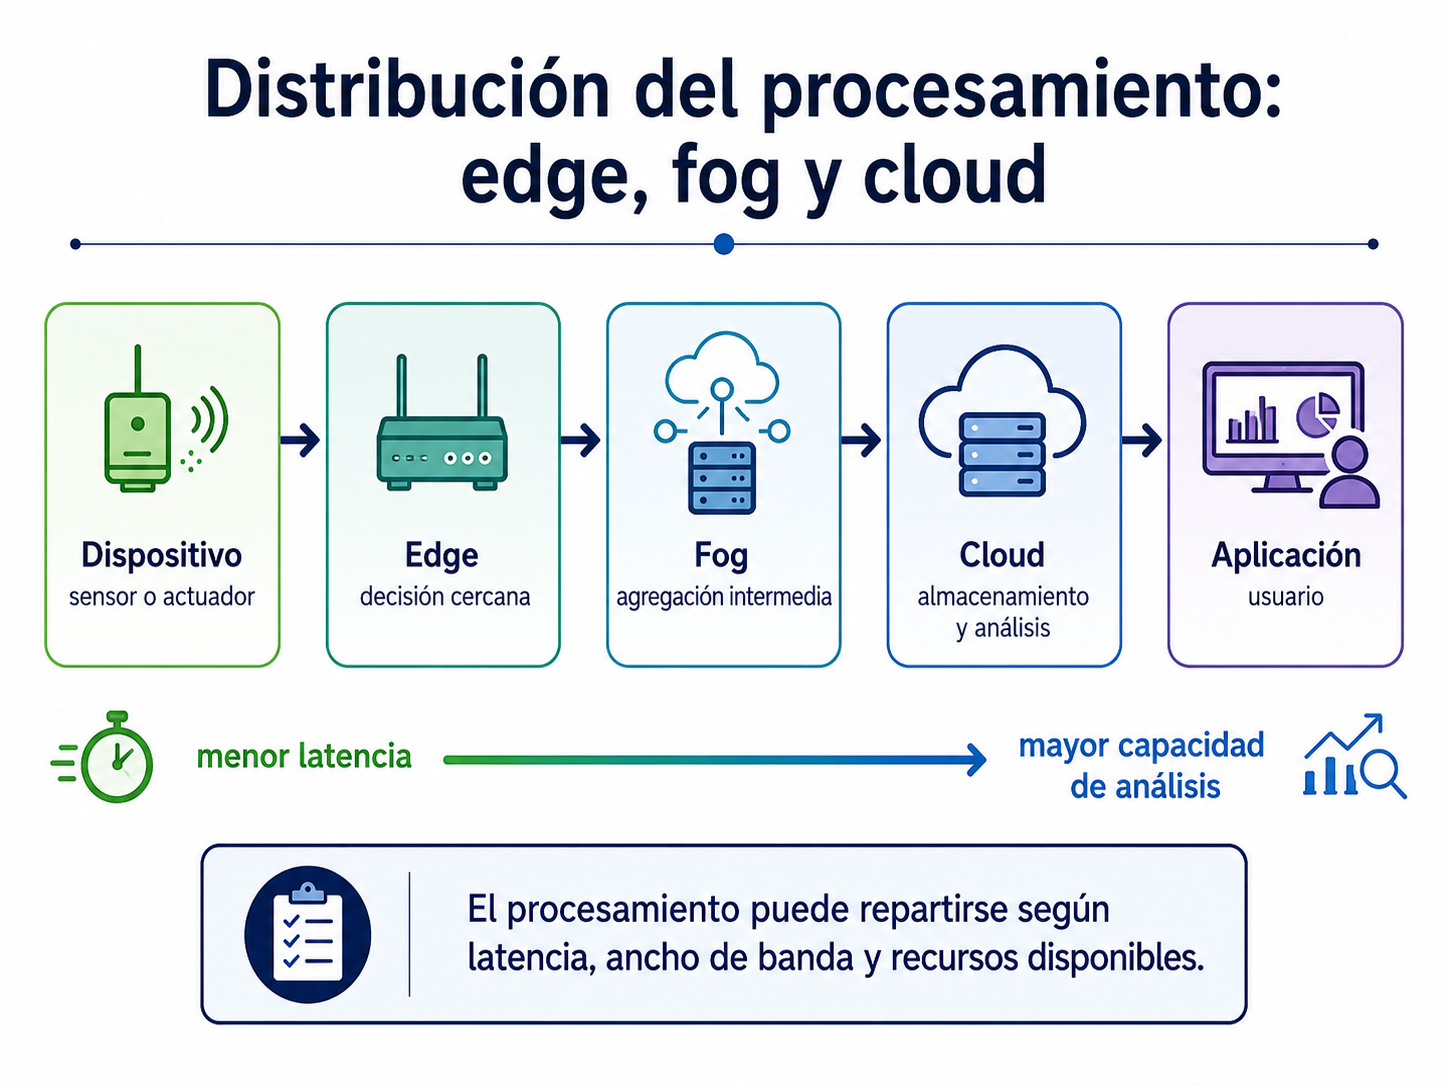
\includegraphics[width=\textwidth]{figs/figura_2_6_edge_fog_cloud.png}
    \caption{Distribución del procesamiento en arquitecturas IoT. Elaboración propia, véase Anexo~\ref{sec:uso_ia_generativa_tfg}.}
    \label{fig:cap2_edge_fog_cloud}
\end{figure}

Una función habitual de estas plataformas es almacenar telemetría, es decir, medidas de sensores, estados de funcionamiento, eventos o errores. Normalmente se organiza como series temporales asociadas a un dispositivo, canal, variable o identificador, de forma que pueda consultarse tanto el último valor como su evolución histórica. Muchas plataformas incorporan además gráficas, paneles de control e indicadores de estado, lo que acelera la validación inicial de prototipos.

Una API (\textit{Application Programming Interface}) es una interfaz programable que una plataforma ofrece para que otros desarrollos software puedan acceder a su funcionalidad de forma controlada. En una plataforma IoT, la API puede permitir escribir telemetría, consultar lecturas, recuperar históricos o integrar esos datos en aplicaciones propias. No debe confundirse la API con el protocolo utilizado para acceder a ella: HTTP, MQTT o CoAP transportan la información, mientras que la API define operaciones, parámetros, autenticación, formatos y respuestas.

ThingSpeak es una plataforma de análisis IoT de la empresa MathWorks\textsuperscript{\textregistered} que permite agregar, visualizar y analizar flujos de datos en la nube \cite{mathworks_thingspeak_product}. Su estructura se basa en canales y campos, y ofrece una interfaz programable documentada para escribir y leer datos mediante mecanismos como HTTP o MQTT \cite{thingspeak_write_data,thingspeak_read_data}. Desde el punto de vista funcional, puede actuar como \textit{broker} de telemetría, ya que recibe datos publicados por dispositivos y los pone a disposición de otros componentes del sistema. En TierraViva, esta función resulta útil porque permite comprobar pronto si las estaciones publican datos correctamente, antes de invertir esfuerzo en una infraestructura \textit{cloud} propia más compleja.

Existen alternativas como Ubidots, Adafruit IO, Blynk, ThingsBoard o una plataforma propia con \textit{broker} MQTT, base de datos y herramienta de visualización \cite{ubidots_basics,adafruit_io_api,blynk_datastreams,thingsboard_telemetry}. La diferencia principal no está solo en la estética de los paneles, sino en la forma de organizar dispositivos, variables, históricos, autenticación, reglas, límites de uso y posibilidades de integración.

El uso de una plataforma \textit{cloud} introduce dependencias: conexión a Internet, disponibilidad del servicio, latencia, límites de frecuencia, histórico disponible y condiciones de uso. Por este motivo, una arquitectura que mantiene la decisión crítica en el nodo de campo reduce la dependencia operativa de la nube. En TierraViva, la pérdida temporal de conectividad puede afectar a la supervisión, pero no debe impedir que la estación mantenga un comportamiento local seguro.

\section{Automatización, reglas e inteligencia artificial en riego}
\label{sec:automatizacion_reglas_ia_riego}

En riego inteligente conviene diferenciar entre automatización basada en reglas e inteligencia artificial (IA). Ambos enfoques pueden utilizar datos procedentes de sensores, pero no toman decisiones del mismo modo. Un sistema automatizado trabaja con condiciones explícitas definidas por el diseñador; un sistema basado en IA requiere modelos entrenados o ajustados a partir de datos históricos suficientes.

La automatización basada en reglas es habitual en prototipos y sistemas de control sencillos. Consiste en definir condiciones del tipo: si una variable supera o cae por debajo de un valor, se ejecuta una acción. En riego, un ejemplo típico sería activar el sistema cuando la humedad del suelo desciende por debajo de un umbral y detenerlo cuando se alcanza una condición de cierre. Este control es fácil de interpretar, validar y explicar. Además, cuando las reglas se ejecutan en el propio nodo de campo, la actuación no depende de una conexión permanente con un servidor externo.

El uso de umbrales debe complementarse con medidas de estabilidad y seguridad. Una única condición puede provocar conmutaciones repetidas si la medida oscila alrededor del valor definido; por ello pueden utilizarse mecanismos como histéresis, confirmación de varias lecturas, tiempo máximo de activación, \textit{cooldown} entre actuaciones, descarte de valores imposibles y comportamiento conservador ante fallos de sensor, alimentación o comunicación.

La inteligencia artificial introduce un enfoque distinto: los modelos pueden aprender patrones a partir de históricos y utilizarlos para predecir humedad del suelo, estimar necesidades de riego o detectar anomalías \cite{abioye2020,bwambale2022}. Sin embargo, para hablar con rigor de IA no basta con utilizar reglas \textit{si-entonces}; sería necesario disponer de datos representativos, seleccionar un modelo, entrenarlo, validarlo y comprobar que aporta valor frente a una estrategia basada en reglas simples.

En agricultura esta exigencia es especialmente importante, ya que los datos dependen del tipo de suelo, clima, estación del año, cultivo, ubicación de los sensores, frecuencia de riego y mantenimiento. Aunque las técnicas de IA aplicadas a sensores agrícolas y monitorización de cultivos tienen potencial \cite{taha2025,naqvi2025}, su uso debe plantearse con prudencia cuando no existe todavía un histórico amplio y fiable.

Para TierraViva, el enfoque basado en reglas verificables es una primera fase razonable. Permite justificar cada actuación, facilita las pruebas y evita atribuir al prototipo capacidades no validadas. En esta versión, cada estación evalúa condiciones simples y seguras, mientras que la Raspberry Pi conserva un papel de supervisión e histórico. La IA queda como línea futura cuando exista un conjunto de datos suficientemente amplio, fiable y representativo.

\chapter{Métodos, materiales y decisiones de diseño}
\label{cap:capitulo3}
Este capítulo concreta el diseño de TierraViva a partir del marco técnico descrito en el capítulo anterior. Aquí se fijan los requisitos del sistema, se explican los criterios de elección y se documentan las decisiones que han guiado el prototipo: qué debe medir cada estación, cómo se comunica, qué papel conserva la Raspberry Pi y qué condiciones deben cumplirse antes de actuar sobre el riego.

A diferencia del estado del arte, el análisis se centra ya en el proyecto desarrollado. Algunas decisiones se tomaron de forma incremental, a medida que se validaban sensores, comunicaciones y software de supervisión. Por ello, el capítulo no se limita a enumerar materiales, sino que justifica por qué TierraViva adopta una arquitectura distribuida con decisión local en las estaciones.

\section{Requisitos funcionales del sistema}
\label{sec:requisitos_funcionales}

Los requisitos funcionales definen las capacidades que debe proporcionar el sistema para cumplir con el alcance planteado para el proyecto. En el caso de TierraViva, estos requisitos no se limitan a la lectura de sensores, sino que cubren el ciclo completo de funcionamiento: adquisición de datos en campo, transmisión remota, almacenamiento, visualización, toma de decisiones y actuación sobre el riego.

La definición de estos requisitos permite separar con claridad qué debe hacer el sistema de cómo se implementa cada parte. Esta distinción es importante porque las decisiones tecnológicas concretas se justifican en apartados posteriores. En este punto se describe el comportamiento esperado del prototipo y la forma prevista de comprobar que cada función queda cubierta durante la validación.

El sistema se plantea a partir de estaciones de campo capaces de obtener medidas del entorno, evaluar localmente reglas sencillas de riego y enviar la información a una plataforma intermedia. A partir de esos datos, el sistema de supervisión debe poder registrar el histórico, visualizar el estado del prototipo y mostrar las actuaciones realizadas por cada estación. La estación de campo debe ejecutar la actuación de forma autónoma y segura, evitando activaciones indefinidas, riegos repetidos o estados peligrosos ante lecturas inválidas, errores de comunicación o fallos eléctricos.

\begin{figure}[H]
    \centering
    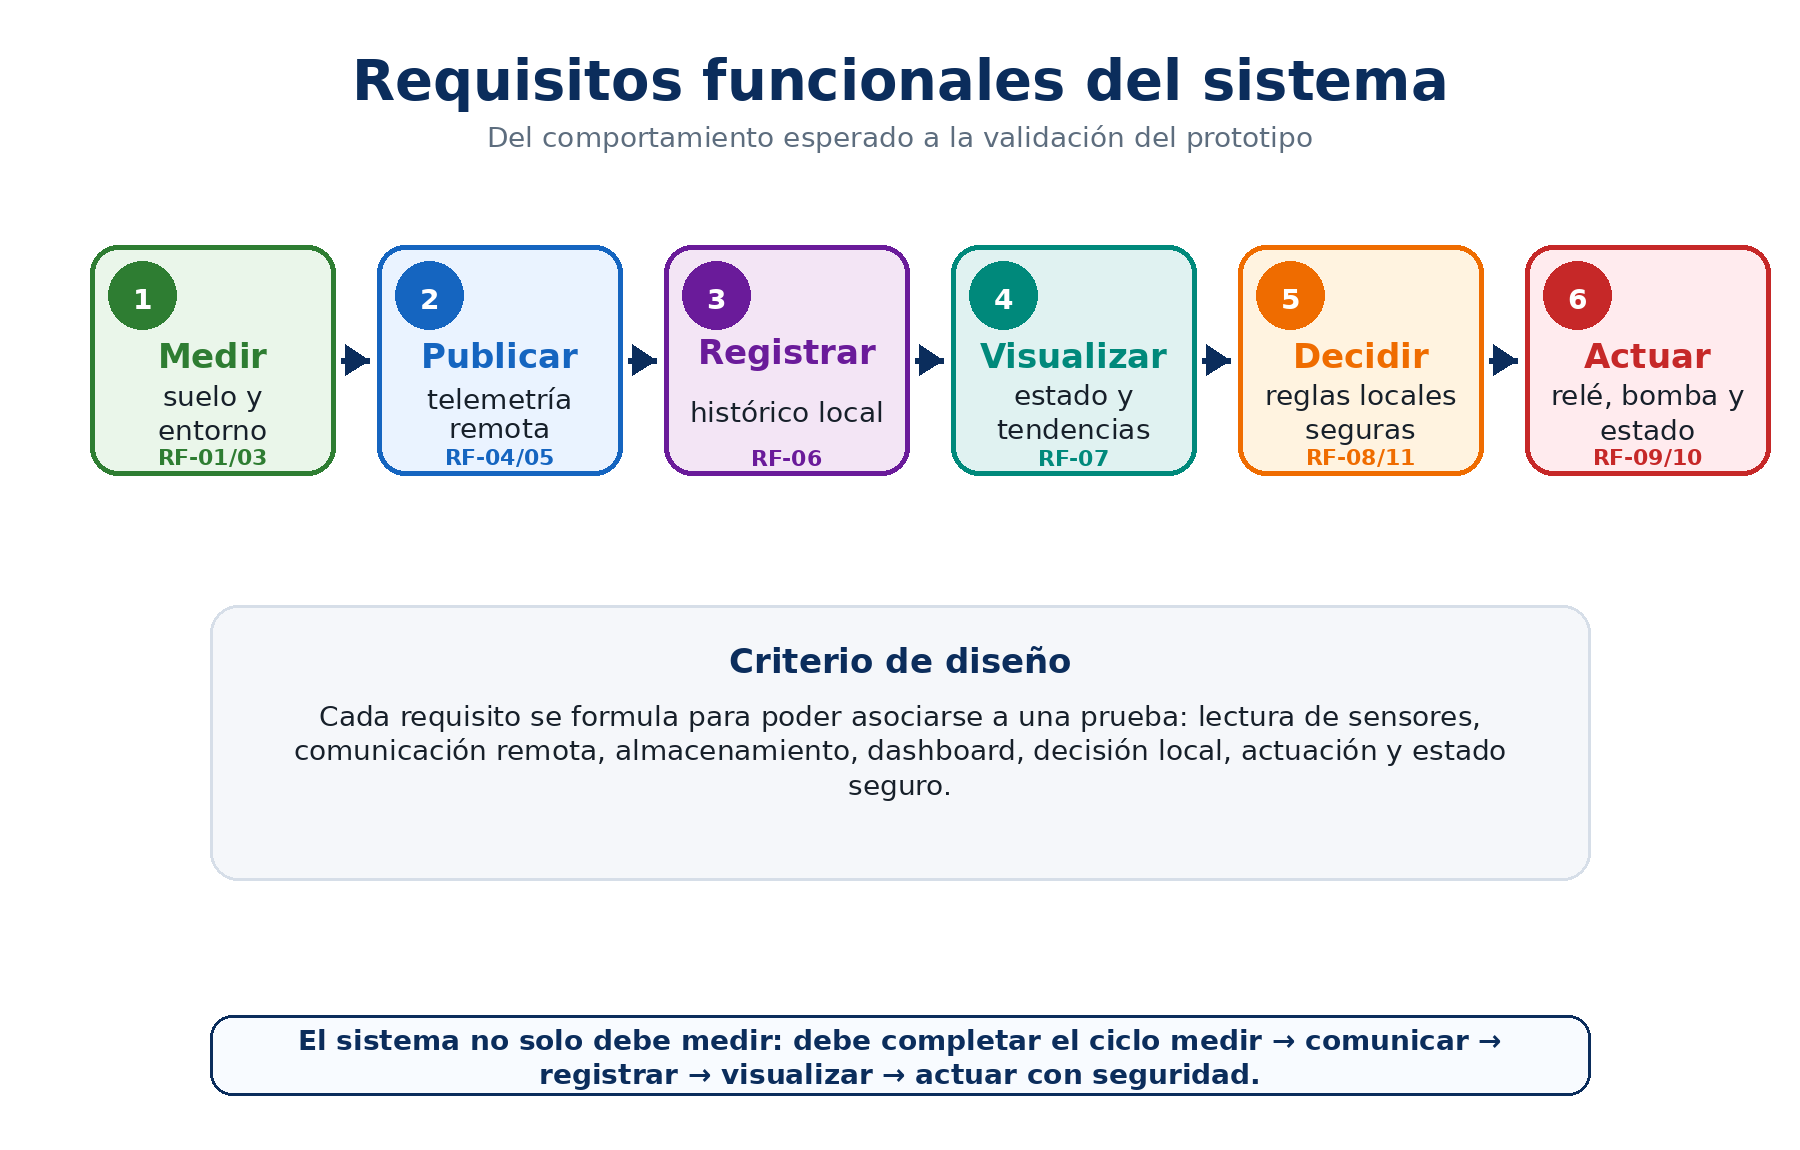
\includegraphics[width=\textwidth]{figs/figura_3_1_requisitos_funcionales.png}
    \caption{Relación entre los requisitos funcionales y el ciclo completo de funcionamiento del sistema. TierraViva debe medir, publicar telemetría, registrar histórico, visualizar el estado, decidir localmente y actuar sobre el riego de forma segura.}
    \label{fig:cap3_requisitos_funcionales}
\end{figure}

En la Tabla~\ref{cuadro:requisitos_funcionales} se recogen los principales requisitos funcionales considerados para el diseño del prototipo.

\begin{table}[H]
\centering
\small
\setlength{\tabcolsep}{4pt}
\renewcommand{\arraystretch}{1.15}
\rowcolors{2}{TableRowSoft}{white}

\makebox[\textwidth][c]{%
\hspace*{-0.7cm}%
\begin{tabular}{|
>{\raggedright\arraybackslash}p{0.06\textwidth}|
>{\raggedright\arraybackslash}p{0.22\textwidth}|
>{\raggedright\arraybackslash}p{0.52\textwidth}|
>{\raggedright\arraybackslash}p{0.24\textwidth}|}
\hline
\rowcolor{URJCRed}
\TVHead{Código} & \TVHead{Requisito} & \TVHead{Descripción} & \TVHead{Validación prevista} \\
\hline
RF-01 & Medición de humedad del suelo & El sistema debe obtener lecturas periódicas de la humedad del sustrato en la zona monitorizada. & Prueba con sensor capacitivo de humedad del suelo. \\
\hline
RF-02 & Medición ambiental & El sistema debe medir variables ambientales relevantes, incluyendo temperatura, humedad relativa y presión atmosférica. & Prueba con sensor ambiental. \\
\hline
RF-03 & Medición de luminosidad & El sistema debe registrar la luminosidad o nivel de luz ambiente para contextualizar las condiciones del entorno. & Prueba con variación de luz. \\
\hline
RF-04 & Envío remoto de telemetría & Las estaciones de campo deben enviar sus medidas a una plataforma remota para que puedan ser consultadas posteriormente. & Prueba de comunicación remota y recepción en plataforma cloud. \\
\hline
RF-05 & Identificación de estación & Cada lectura debe poder asociarse a la estación de origen, permitiendo distinguir los datos de distintas zonas o nodos. & Comprobación de registros diferenciados por estación. \\
\hline
RF-06 & Almacenamiento histórico & El sistema debe registrar las lecturas recibidas para conservar un histórico de funcionamiento. & Verificación de inserciones en SQLite. \\
\hline
RF-07 & Visualización del estado & El sistema debe ofrecer una interfaz de consulta que permita ver las últimas lecturas y el estado general del prototipo. & Prueba de dashboard web en navegador. \\
\hline
RF-08 & Decisión local de riego & Cada estación debe evaluar localmente si las condiciones medidas justifican una actuación sobre el riego. & Prueba de regla local de humedad, cooldown y estado seguro. \\
\hline
RF-09 & Actuación local sobre el riego & La estación debe accionar físicamente el sistema de riego mediante relé y bomba de agua durante un tiempo limitado por firmware. & Prueba controlada con relé y bomba/carga de prueba. \\
\hline
RF-10 & Publicación de estado de actuación & La estación debe publicar el estado del relé, el evento de sistema y un código auxiliar de diagnóstico que permitan conocer si se ha producido una actuación, una situación de reposo, un error, un estado seguro o un bloqueo por cooldown. & Verificación de \texttt{relay\_state}, \texttt{system\_event} y \texttt{debug\_code} en ThingSpeak. \\
\hline
RF-11 & Seguridad de funcionamiento & El sistema debe desactivar o mantener apagada la bomba ante error de sensor, lectura inválida, fallo de comunicación, reinicio, cooldown activo o tiempo máximo excedido. & Pruebas de modo seguro, reinicio y límites de actuación. \\
\hline
\end{tabular}%
}

\caption{Requisitos funcionales del sistema TierraViva}
\label{cuadro:requisitos_funcionales}
\end{table}

Los requisitos funcionales se agrupan en cuatro bloques. Los requisitos RF-01 a RF-03 cubren la adquisición de información en campo mediante sensores de suelo y ambiente. Los requisitos RF-04 a RF-07 definen el flujo de datos hacia la plataforma intermedia, el almacenamiento histórico y la visualización. Por último, RF-08, RF-09 y RF-10 incorporan la decisión local de riego, la actuación física y la publicación del estado operativo de cada estación.

El requisito RF-11 se ha incluido de forma explícita porque TierraViva no se limita a monitorizar variables, sino que actúa sobre una bomba de agua. Por ello, el sistema debe adoptar un comportamiento conservador ante lecturas inválidas, reinicios, fallos de comunicación o estados no verificables.

La relación completa entre requisitos, pruebas y evidencias de validación se desarrolla en el Anexo~\ref{anexo:trazabilidad_requisitos_pruebas}. De este modo, el cuerpo principal conserva la definición del sistema y los anexos recogen la comprobación detallada.

\section{Requisitos no funcionales}
\label{sec:requisitos_no_funcionales}

Los requisitos no funcionales describen las condiciones de calidad que debe cumplir el sistema, más allá de las funciones concretas indicadas en el apartado anterior. En TierraViva estos requisitos son especialmente importantes porque el proyecto no consiste únicamente en que cada bloque funcione de forma aislada, sino en que el conjunto pueda integrarse, probarse, ampliarse y defenderse como un prototipo de ingeniería.

El sistema debe mantener un equilibrio entre ambición técnica y viabilidad. No se pretende desarrollar un producto industrial cerrado, pero sí una solución suficientemente robusta, ordenada y reproducible como para demostrar el funcionamiento completo de la arquitectura propuesta. La Tabla~\ref{cuadro:requisitos_no_funcionales} resume los principales requisitos no funcionales considerados.

\begin{figure}[H]
    \centering
    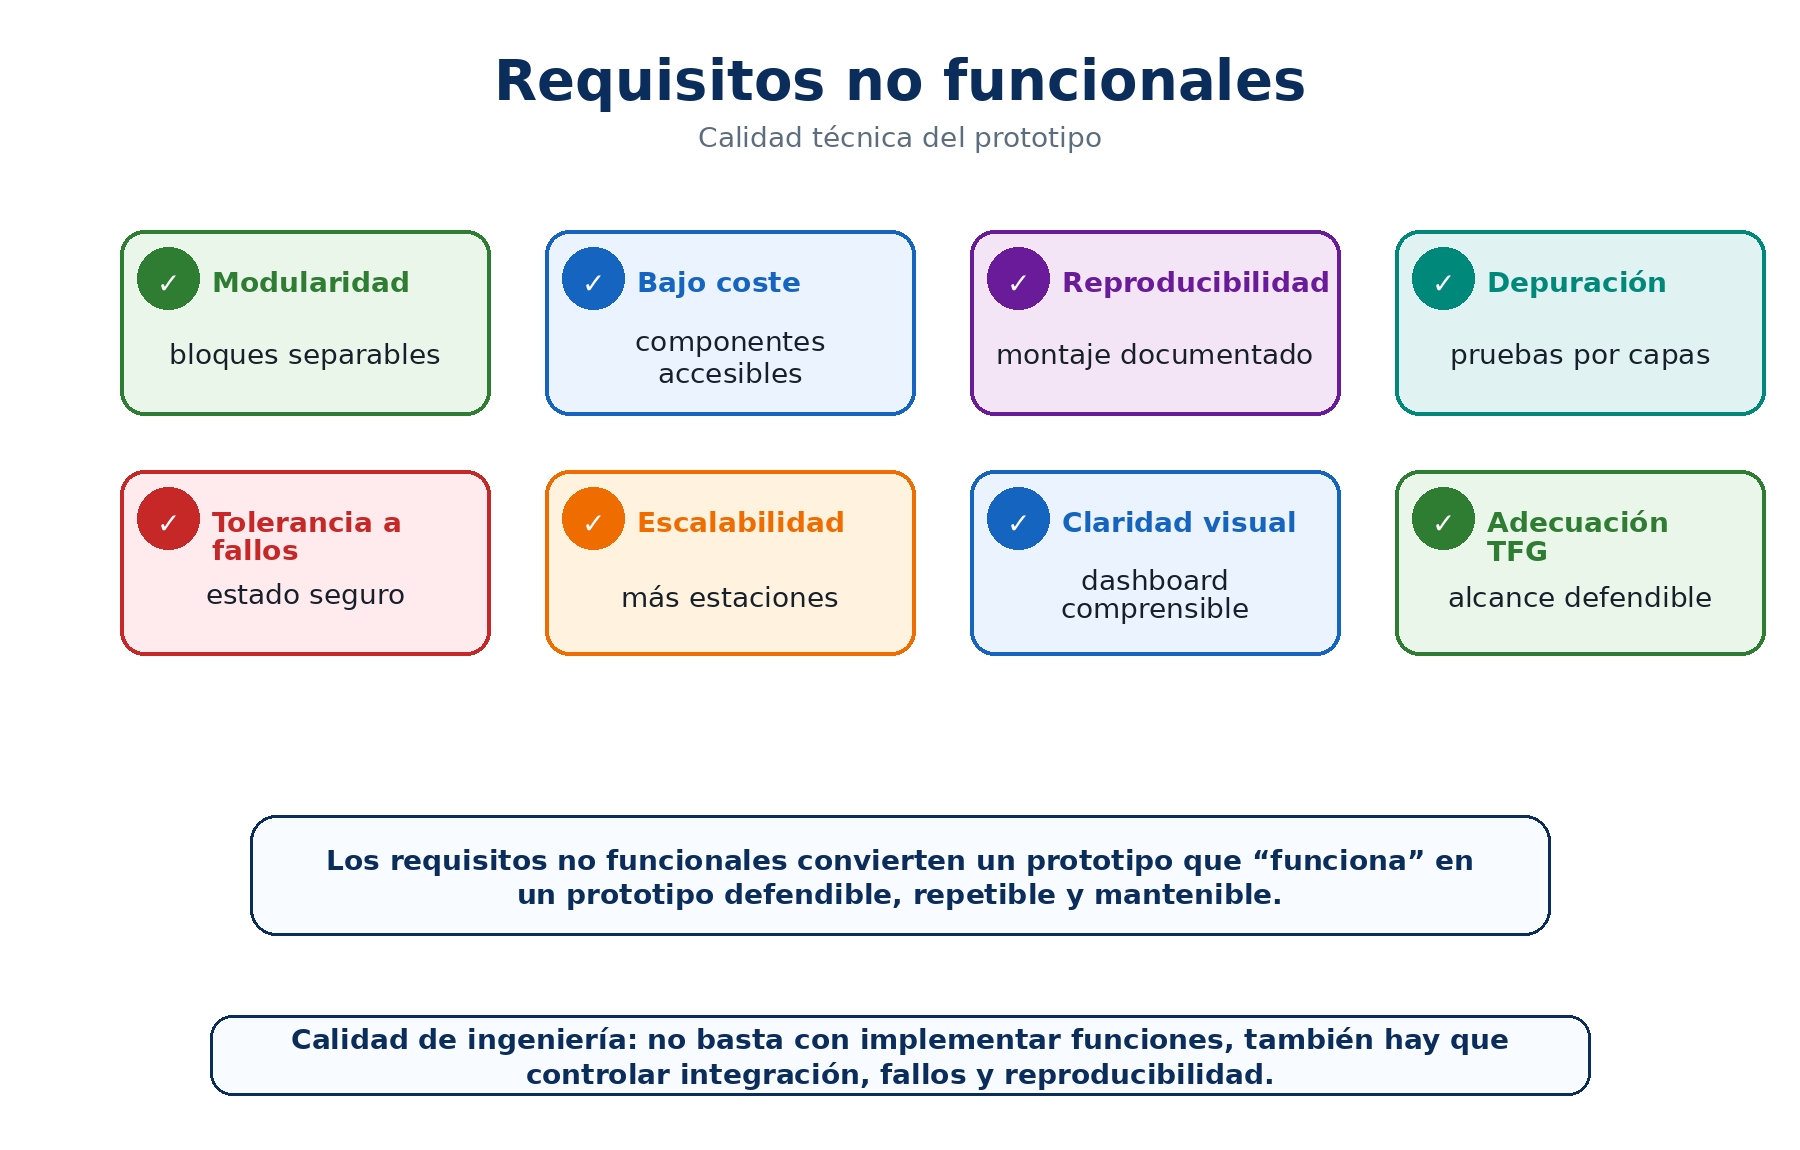
\includegraphics[width=\textwidth]{figs/figura_3_2_requisitos_no_funcionales.png}
    \caption{Requisitos no funcionales considerados en el diseño del prototipo. Estos criterios permiten evaluar la calidad técnica del sistema más allá de las funciones implementadas.}
    \label{fig:cap3_requisitos_no_funcionales}
\end{figure}

\begin{table}[H]
\begin{center}
\small
\renewcommand{\arraystretch}{1.15}
\rowcolors{2}{TableRowSoft}{white}

\begin{tabular}{|p{0.13\textwidth}|p{0.25\textwidth}|p{0.50\textwidth}|}
\hline
\rowcolor{URJCRed}
\TVHead{Código} & \TVHead{Requisito} & \TVHead{Descripción} \\
\hline
RNF-01 & Modularidad & El sistema debe organizarse en bloques diferenciados: estación de campo autónoma, comunicación, almacenamiento, supervisión, visualización y actuación local. \\
\hline
RNF-02 & Bajo coste & Los componentes seleccionados deben ser asumibles para un prototipo académico, evitando soluciones industriales de coste elevado cuando no sean necesarias. \\
\hline
RNF-03 & Reproducibilidad & El montaje, la configuración y las pruebas deben poder repetirse a partir de la documentación generada durante el proyecto. \\
\hline
RNF-04 & Facilidad de depuración & El sistema debe permitir probar los bloques por separado, identificar errores y consultar salidas intermedias durante el desarrollo. \\
\hline
RNF-05 & Consumo razonable & El diseño debe evitar consumos innecesarios y permitir una futura alimentación autónoma, aunque la optimización energética completa no sea el objetivo principal. \\
\hline
RNF-06 & Tolerancia a fallos & El sistema debe contemplar fallos de lectura, comunicación o actuación, adoptando estados seguros cuando no sea posible garantizar un funcionamiento correcto. \\
\hline
RNF-07 & Escalabilidad & La arquitectura debe permitir incorporar más de una estación de campo sin rediseñar completamente el sistema. \\
\hline
RNF-08 & Claridad de visualización & La interfaz debe presentar la información de forma comprensible, diferenciando lecturas, estados y posibles incidencias. \\
\hline
RNF-09 & Adecuación académica & El alcance debe ser realizable dentro del tiempo y medios disponibles para el TFG, priorizando funciones verificables frente a desarrollos excesivamente complejos. \\
\hline
\end{tabular}
\caption{Requisitos no funcionales del sistema TierraViva}
\label{cuadro:requisitos_no_funcionales}
\end{center}
\end{table}

Estos requisitos no funcionales condicionan la arquitectura del proyecto. La modularidad, la reproducibilidad y la facilidad de depuración justifican la separación entre estación de campo, plataforma intermedia, Raspberry Pi, API y dashboard. Esta división permite probar cada bloque de forma independiente y reduce el riesgo de que un fallo en una capa impida validar el conjunto.

El bajo coste y la adecuación académica orientan la selección de componentes hacia módulos accesibles, documentados y suficientes para demostrar el funcionamiento del sistema. La escalabilidad se plantea de forma limitada pero necesaria: el sistema debe poder trabajar con más de una estación sin rediseñar por completo la arquitectura.

La tolerancia a fallos y el consumo razonable son especialmente relevantes por la presencia de actuación física. La estación debe mantener un comportamiento seguro ante errores de lectura, comunicación o alimentación, y el diseño debe dejar abierta la posibilidad de una alimentación autónoma en futuras versiones. El análisis ampliado de riesgos se recoge en el Anexo~\ref{anexo:gestion_riesgos}.

\section{Especificaciones temporales y operativas}
\label{sec:especificaciones_temporales_operativas}

Además de los requisitos funcionales y no funcionales, el sistema necesita definir una serie de parámetros temporales y criterios operativos que regulen su comportamiento durante el funcionamiento. En un sistema IoT de riego, estos valores son importantes porque afectan al consumo energético, a la carga de comunicaciones, a la capacidad de respuesta y, sobre todo, a la seguridad de la actuación sobre la bomba de agua.

Las especificaciones temporales no se plantean como valores rígidos e inmodificables, sino como parámetros iniciales de diseño. Durante el desarrollo y la validación del prototipo pueden ajustarse en función de los resultados obtenidos, siempre manteniendo dos criterios principales: evitar comunicaciones innecesarias y garantizar que cualquier actuación sobre el riego quede limitada en el tiempo.

\begin{figure}[H]
    \centering
    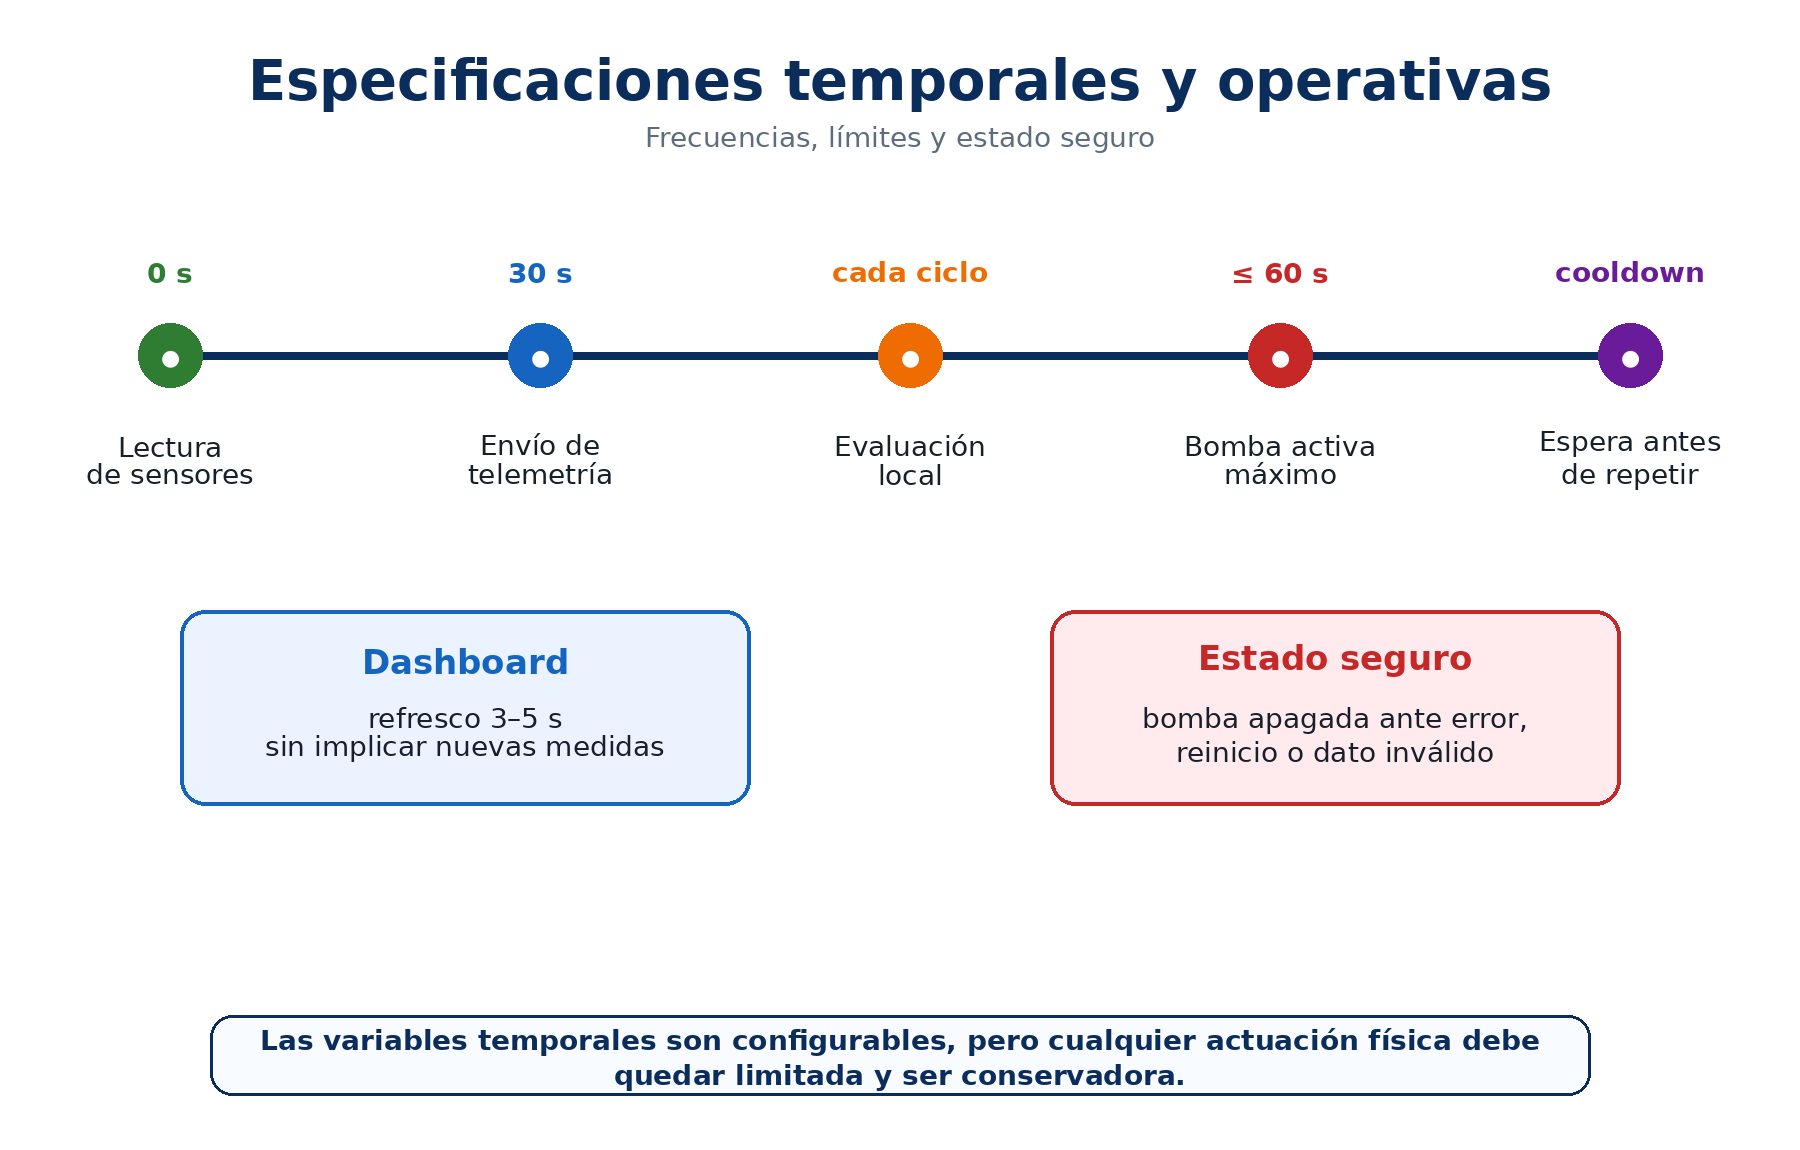
\includegraphics[width=0.85\textwidth]{figs/figura_3_3_especificaciones_temporales.png}
    \caption{Especificaciones temporales y operativas iniciales del sistema.}
    \label{fig:cap3_especificaciones_temporales}
\end{figure}

En la Tabla~\ref{cuadro:especificaciones_temporales} se recogen las principales especificaciones temporales y operativas consideradas para TierraViva.

\begin{table}[H]
\centering
\footnotesize
\renewcommand{\arraystretch}{1.15}
\rowcolors{2}{TableRowSoft}{white}

\makebox[\textwidth][c]{%
\hspace*{-0.7cm}%
\begin{tabular}{|
>{\raggedright\arraybackslash}p{0.09\textwidth}|
>{\raggedright\arraybackslash}p{0.28\textwidth}|
>{\raggedright\arraybackslash}p{0.17\textwidth}|
>{\raggedright\arraybackslash}p{0.38\textwidth}|}
\hline
\rowcolor{URJCRed}
\TVHead{Código} & \TVHead{Parámetro} & \TVHead{Valor inicial} & \TVHead{Criterio operativo} \\
\hline
ET-01 & Periodo de lectura de sensores & Configurable & Las estaciones toman medidas periódicas del entorno. Durante pruebas pueden utilizarse intervalos reducidos para acelerar la validación. \\
\hline
ET-02 & Frecuencia de envío de telemetría & Configurable & Cada estación envía sus datos de forma periódica, evitando tráfico innecesario en funcionamiento normal. \\
\hline
ET-03 & Frecuencia de actualización del dashboard & 3--5 s & La interfaz consulta el estado con mayor frecuencia que la llegada real de nuevos datos. \\
\hline
ET-04 & Intervalo de evaluación local & Configurable & Cada estación evalúa periódicamente sus lecturas y comprueba si se cumplen las condiciones locales de riego. \\
\hline
ET-05 & Tiempo máximo de bomba activa & Configurable & La activación de la bomba queda limitada por firmware para evitar riego indefinido ante errores de control. \\
\hline
ET-06 & Tiempo mínimo entre riegos & Configurable & Se aplica un periodo de espera para evitar actuaciones repetidas en poco tiempo. \\
\hline
ET-07 & Tiempo máximo sin dato reciente en supervisión & Configurable & La Raspberry Pi y el dashboard deben identificar lecturas antiguas u offline cuando no se reciben publicaciones recientes de una estación. \\
\hline
ET-08 & Estado seguro por defecto & Bomba apagada & Al arrancar, ante error de lectura, fallo de comunicación o condición no verificable, la estación mantiene desactivado el riego. \\
\hline
ET-09 & Comportamiento ante dato inválido & Ignorar y registrar & Las lecturas no válidas no deben provocar una actuación automática. \\
\hline
ET-10 & Comportamiento ante pérdida de comunicación & Bomba apagada o no actuación & La pérdida de comunicación no debe dejar la bomba activa. \\
\hline
\end{tabular}%
}

\caption{Especificaciones temporales y operativas iniciales del sistema}
\label{cuadro:especificaciones_temporales}
\end{table}

Los parámetros temporales se definen como valores configurables del firmware. Durante las pruebas pueden emplearse intervalos reducidos para acelerar la validación, mientras que en un funcionamiento más estable conviene utilizar periodos más conservadores. Lo importante desde el punto de vista de diseño no es fijar un único valor definitivo, sino garantizar ciclos controlados, detección de datos antiguos en supervisión y actuación de la bomba siempre limitada temporalmente.

La actualización del dashboard puede realizarse con mayor frecuencia que la publicación de las estaciones, pero no debe interpretarse como una nueva medida en cada refresco. La actuación física queda gobernada por el firmware de la estación, que debe mantener la bomba apagada ante lecturas inválidas, reinicios, pérdida de comunicación o estados no verificables.

\section{Metodología de trabajo}
\label{sec:metodologia_trabajo}

La metodología seguida en TierraViva se ha basado en un desarrollo incremental por bloques. En lugar de intentar construir el sistema completo desde el primer momento, se ha dividido el proyecto en fases más pequeñas, cada una orientada a validar una parte concreta de la arquitectura. Este enfoque resulta adecuado para un sistema IoT con sensores, comunicaciones, almacenamiento, visualización y actuación física, ya que permite aislar errores y reducir el riesgo de integración.

La idea principal ha sido avanzar desde pruebas controladas hacia una arquitectura cada vez más cercana al funcionamiento final. Primero se analizaron las necesidades del problema y las alternativas tecnológicas disponibles. Después se desarrollaron prototipos parciales para comprobar sensores, comunicaciones, almacenamiento y visualización. Finalmente, las distintas partes se fueron conectando hasta formar una solución de monitorización y control más completa.

Esta forma de trabajo también ha permitido documentar decisiones y cambios de enfoque. En un proyecto de este tipo, no todas las decisiones se pueden cerrar desde el principio, ya que algunas dependen de la disponibilidad real de hardware, de la facilidad de integración o de los resultados obtenidos en pruebas. Por ello, la metodología no se ha limitado a implementar una arquitectura previamente fija, sino que ha incorporado revisión, validación y corrección de decisiones durante el desarrollo.

En la Tabla~\ref{cuadro:metodologia_fases} se resumen las fases principales seguidas durante el proyecto.

\begin{table}[H]
\centering
\footnotesize
\renewcommand{\arraystretch}{1.15}
\rowcolors{2}{TableRowSoft}{white}

\makebox[\textwidth][c]{%
\hspace*{-0.7cm}%
\begin{tabular}{|
>{\raggedright\arraybackslash}p{0.07\textwidth}|
>{\raggedright\arraybackslash}p{0.24\textwidth}|
>{\raggedright\arraybackslash}p{0.68\textwidth}|}
\hline
\rowcolor{URJCRed}
\TVHead{Fase} & \TVHead{Nombre} & \TVHead{Objetivo principal} \\
\hline
1 & Análisis inicial del problema & Identificar la necesidad de monitorizar y controlar el riego en un entorno no supervisado de forma continua. \\
\hline
2 & Revisión tecnológica & Estudiar alternativas de sensorización, plataformas embebidas, comunicaciones, almacenamiento, visualización y actuación. \\
\hline
3 & Diseño conceptual de la arquitectura & Definir los bloques principales del sistema y la relación entre estaciones autónomas de campo, plataforma intermedia, sistema de supervisión y actuador. \\
\hline
4 & Prototipo local con Raspberry & Validar una primera cadena de adquisición, mensajería, almacenamiento y visualización mediante Raspberry Pi, MQTT, SQLite, FastAPI y dashboard. \\
\hline
5 & Validación de sensores & Comprobar el funcionamiento de los sensores de humedad de suelo, luminosidad y variables ambientales antes de integrarlos en una estación. \\
\hline
6 & Validación de comunicaciones & Probar la comunicación remota necesaria para publicar telemetría y estado desde las estaciones. \\
\hline
7 & Elección de plataforma cloud & Seleccionar una plataforma intermedia que permitiera publicar telemetría, consultar datos remotos y supervisar el estado de las estaciones de forma sencilla y verificable. \\
\hline
8 & Diseño de actuación local & Definir el control autónomo de la bomba de agua mediante relé, incluyendo reglas locales, tiempos máximos, cooldown y estado seguro. \\
\hline
9 & Integración de subsistemas & Conectar adquisición, comunicación, supervisión, almacenamiento, visualización, decisión local y actuación en una arquitectura coherente. \\
\hline
10 & Validación experimental & Comprobar el funcionamiento del sistema mediante pruebas parciales, pruebas de estación autónoma y pruebas de supervisión extremo a extremo. \\
\hline
11 & Documentación de incidencias y decisiones & Registrar problemas encontrados, alternativas descartadas, cambios de enfoque y criterios técnicos adoptados. \\
\hline
\end{tabular}%
}

\caption{Fases principales de la metodología de trabajo}
\label{cuadro:metodologia_fases}
\end{table}

Las primeras fases permitieron transformar la necesidad inicial en requisitos técnicos y revisar las alternativas de sensorización, comunicaciones, plataformas embebidas, almacenamiento y visualización. A partir de esa revisión se definió una arquitectura por bloques, con estaciones autónomas de campo, plataforma intermedia, sistema de supervisión y actuación local.

El prototipo local previo con Raspberry Pi permitió validar una primera cadena de adquisición, almacenamiento, API y dashboard antes de adoptar la arquitectura final con LTE y ThingSpeak. Posteriormente se validaron sensores, comunicaciones y actuación por separado, evitando mezclar problemas de cableado, alimentación, módem, backend o lógica de riego en una única fase de integración.

La integración final conectó adquisición, publicación de telemetría, almacenamiento local, visualización, decisión local y actuación sobre el relé. Durante este proceso se documentaron incidencias, alternativas descartadas y cambios de enfoque, especialmente la separación entre supervisión y control local. Esta decisión trasladó la lógica crítica de riego al firmware de cada estación y dejó la Raspberry Pi como sistema de consulta, histórico y visualización.

\section{Arquitectura general planteada}
\label{sec:arquitectura_general_planteada}

A partir de los requisitos definidos en los apartados anteriores, la arquitectura general de TierraViva se plantea como un sistema IoT distribuido, formado por estaciones autónomas de campo, una plataforma intermedia de comunicación y un sistema de supervisión basado en Raspberry Pi. El objetivo de esta arquitectura es separar claramente la adquisición de datos, la decisión local, la actuación física, la publicación de telemetría, el almacenamiento histórico y la visualización.

La arquitectura se ha diseñado teniendo en cuenta una restricción importante: las estaciones de campo no están conectadas físicamente a la Raspberry Pi. Por tanto, no se puede asumir una comunicación directa mediante USB, puerto serie o red local entre ambos extremos. Las estaciones deben poder enviar datos de forma remota mediante el módulo LTE, y la Raspberry debe consultar esa información desde la plataforma intermedia. Esto condiciona el diseño completo del sistema y evita que el riego dependa de una conexión local o de una orden enviada desde la Raspberry.

En términos generales, el sistema se divide en cuatro bloques principales:

\begin{itemize}
    \item \textbf{Estaciones autónomas de campo}: encargadas de medir las variables del entorno, evaluar reglas locales de riego, accionar la bomba mediante relé y publicar telemetría y estado.
    \item \textbf{Capa de comunicaciones y plataforma intermedia}: responsable de recibir los datos publicados por las estaciones y hacerlos accesibles para consulta remota.
    \item \textbf{Sistema de supervisión}: implementado sobre Raspberry Pi, encargado de consultar datos, almacenarlos, exponer una API y servir el dashboard.
    \item \textbf{Interfaz de usuario}: orientada a visualizar el estado del sistema, revisar el histórico y supervisar las actuaciones realizadas por las estaciones.
\end{itemize}

La Figura~\ref{fig:arquitectura_general_tierraviva} muestra una visión general de la arquitectura planteada.

\begin{figure}[H]
  \hspace{-0.5cm}\centerline{\resizebox{1.2\textwidth}{!}{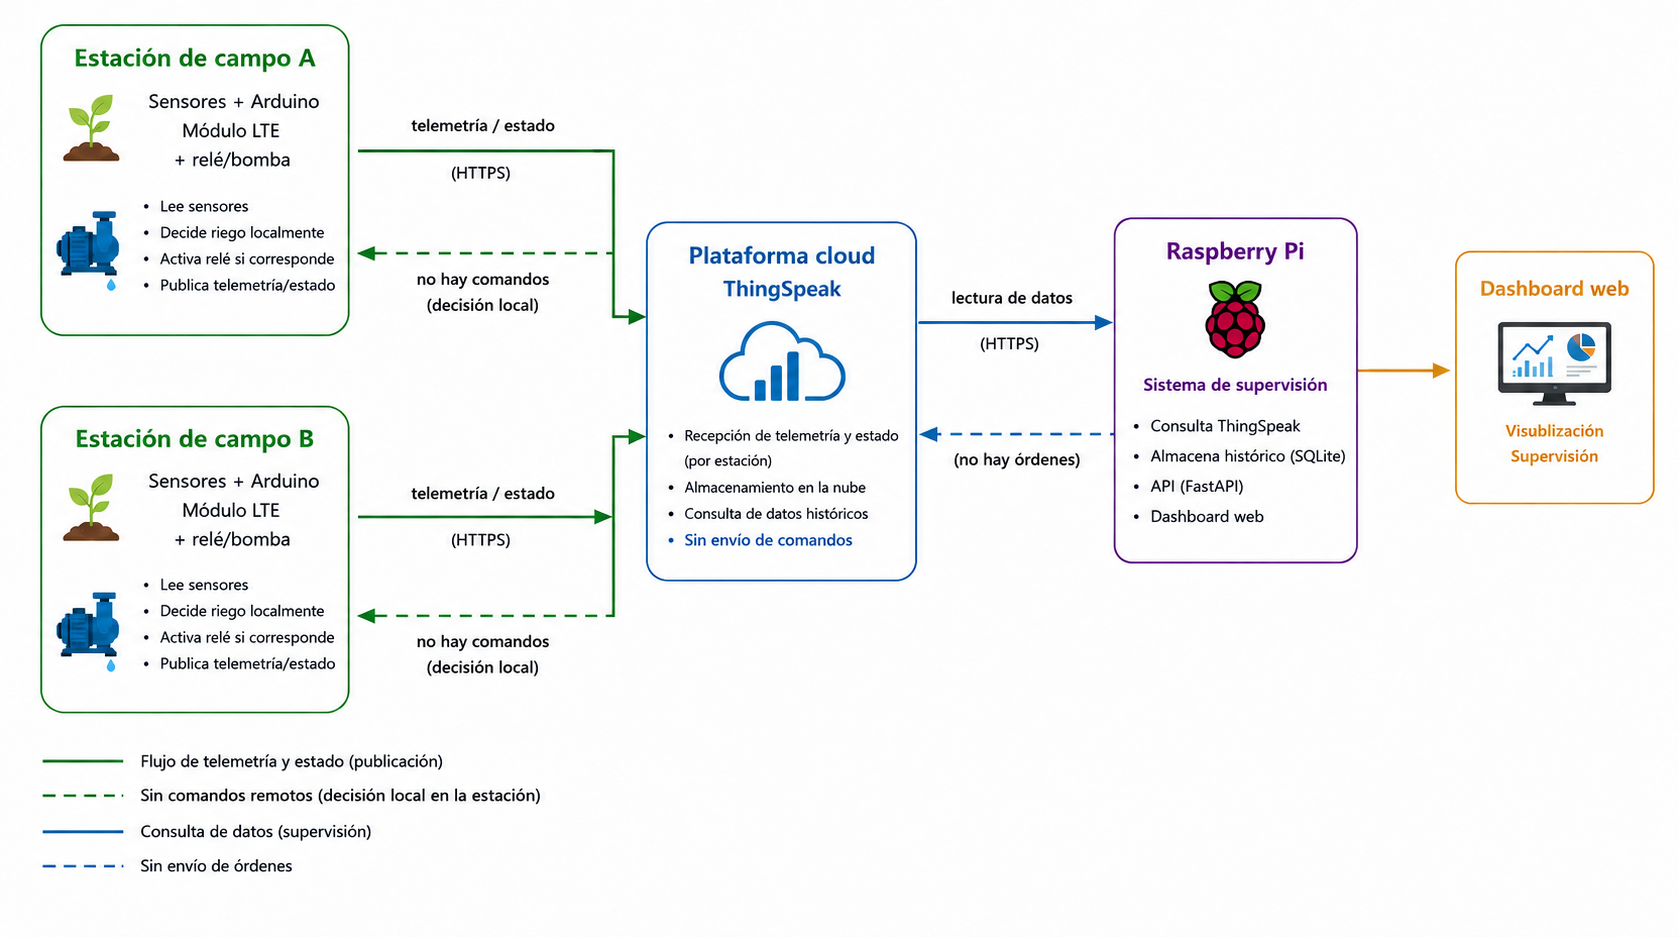
\includegraphics{figs/arquitecturaTierraViva.png}}}
  \caption{Arquitectura general planteada para TierraViva.}
\label{fig:arquitectura_general_tierraviva}
\end{figure}

La división de responsabilidades es el punto central de esta arquitectura. Las estaciones de campo interactúan con el entorno físico, toman la decisión local de riego y publican telemetría. ThingSpeak actúa como plataforma intermedia de comunicación. La Raspberry Pi consulta los datos, mantiene el histórico, expone la API y sirve el dashboard, sin convertirse en el elemento responsable de decidir la activación de la bomba.

El detalle de la arquitectura final, incluyendo canales de ThingSpeak, flujo de telemetría y papel de cada bloque, se desarrolla en el Capítulo~\ref{cap:capitulo4}. Los flujos visuales de funcionamiento se recogen en el Anexo~\ref{anexo:diagramas_flujo_funcionamiento}.

\section{Elección de variables y sensores}
\label{sec:eleccion_variables_sensores}

La selección de variables medidas se ha realizado teniendo en cuenta el papel que deben cumplir dentro del prototipo: monitorizar el estado de una zona de cultivo y aportar información suficiente para alimentar la decisión local de riego en cada estación. No se pretende medir todos los parámetros agronómicos posibles, sino elegir un conjunto reducido de variables que permita validar el comportamiento del prototipo de forma razonable, reproducible y coherente con el alcance del TFG.

En TierraViva se combinan variables del suelo y variables ambientales. La humedad del suelo se considera la variable principal para la decisión local de riego, ya que aporta información directa sobre la disponibilidad de agua en el sustrato. Las variables ambientales, como temperatura, humedad relativa, presión atmosférica y luminosidad, no sustituyen a la humedad del suelo, pero ayudan a interpretar el contexto en el que evoluciona la zona monitorizada. Esta combinación es habitual en sistemas de agricultura de precisión basados en sensores, donde el interés no está solo en una lectura aislada, sino en la observación conjunta del entorno \cite{soussi2024smart}.

\begin{figure}[H]
    \centering
    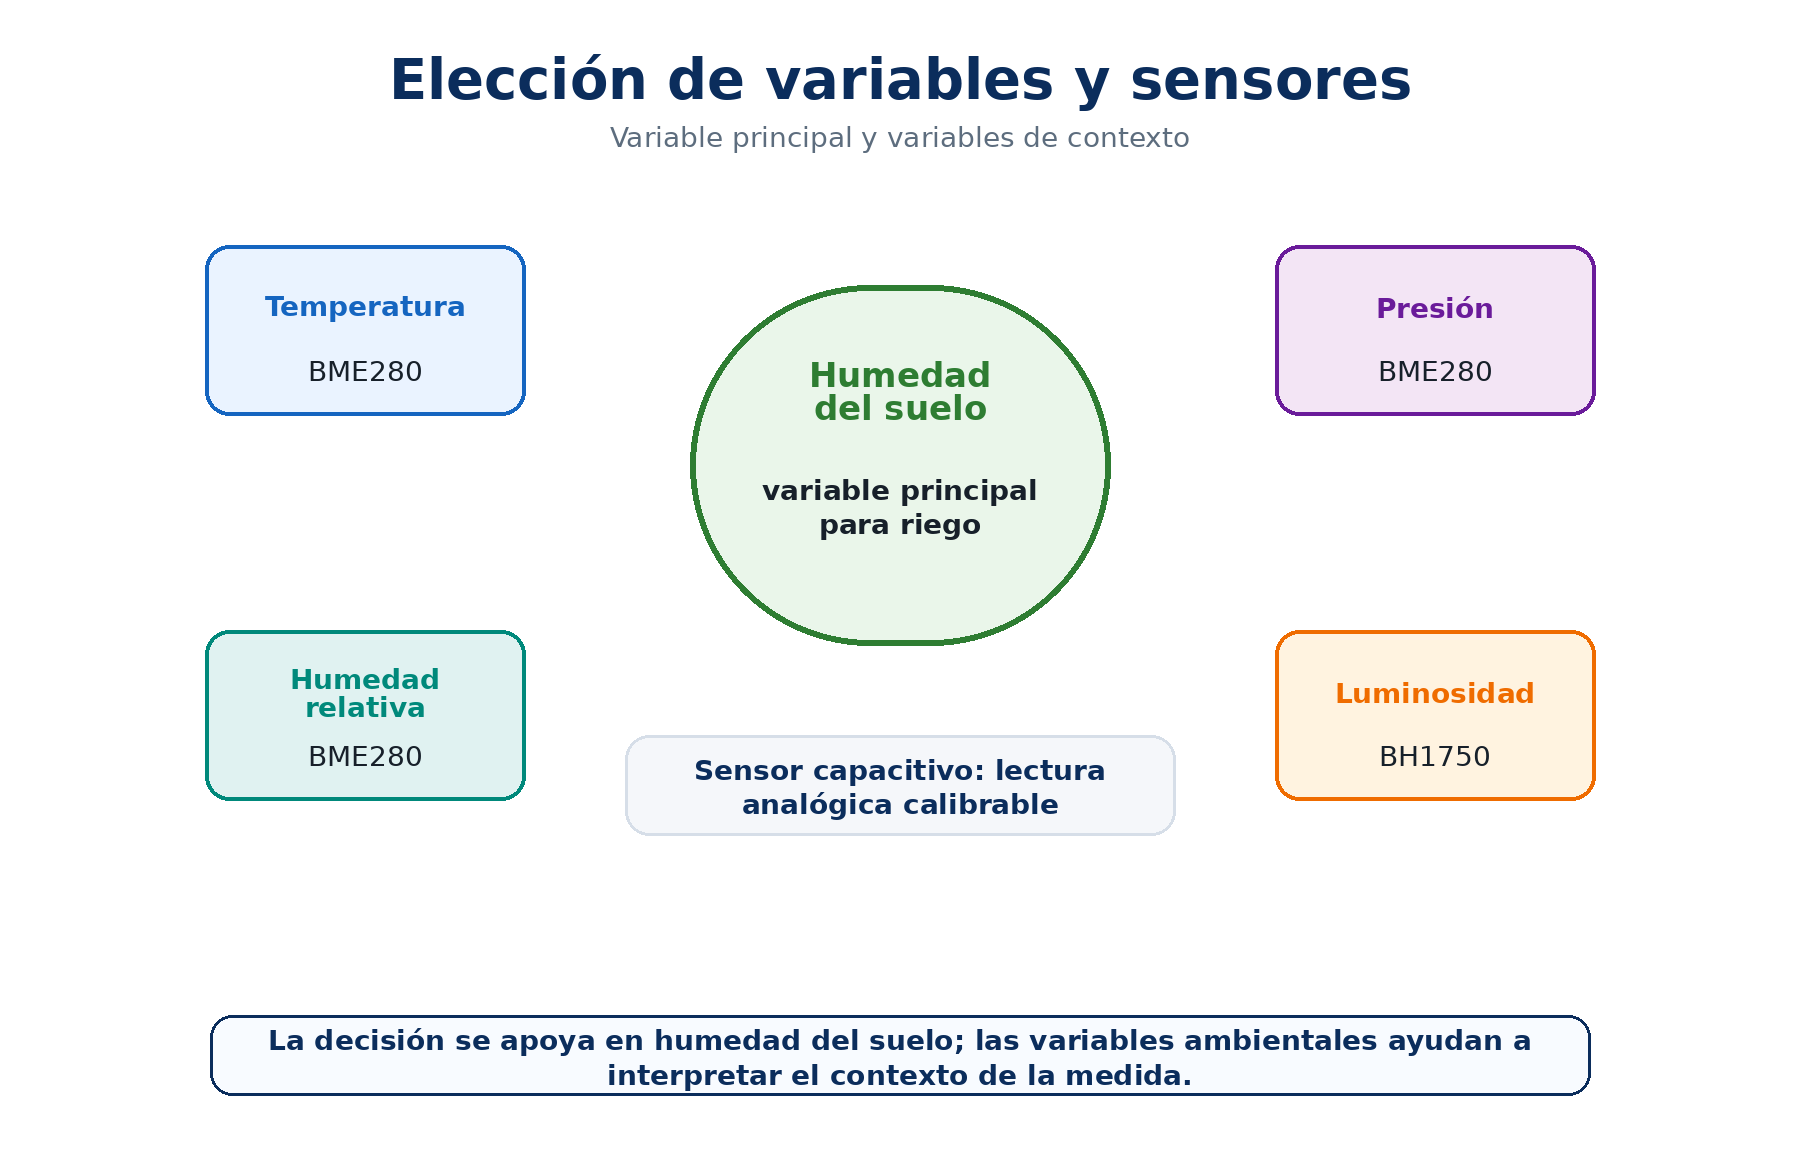
\includegraphics[width=\textwidth]{figs/figura_3_6_variables_sensores.png}
    \caption{Variables seleccionadas para la monitorización de TierraViva. La humedad del suelo se utiliza como variable principal para la decisión local de riego, mientras que temperatura, humedad relativa, presión y luminosidad aportan contexto ambiental.}
    \label{fig:cap3_variables_sensores}
\end{figure}

La Figura~\ref{fig:cap3_variables_sensores} resume las variables seleccionadas. La humedad del suelo actúa como variable principal de decisión, mientras que temperatura, humedad relativa, presión atmosférica y luminosidad aportan contexto ambiental. La correspondencia entre sensores y magnitudes medidas se recoge en la Tabla~\ref{cuadro:sensores_seleccionados}.

La humedad del suelo se ha seleccionado como variable principal porque es la medida más directamente relacionada con la necesidad de riego. En el prototipo se utiliza un sensor capacitivo de humedad de suelo V1.2, cuya salida analógica permite integrarlo de forma sencilla con Arduino. Frente a sensores resistivos, este tipo de sensor reduce los problemas de degradación por contacto con humedad, aunque requiere calibración para interpretar sus valores como porcentaje útil de humedad \cite{azdelivery_soil_v12}.

Las variables ambientales se incorporan como información de contexto. La temperatura, la humedad relativa y la presión se obtienen mediante el BME280, que integra las tres magnitudes en un único módulo digital con comunicación I2C \cite{bosch_bme280_datasheet}. La luminosidad se mide mediante el BH1750/GY-302, que proporciona valores en lux y permite interpretar la exposición solar de la zona monitorizada \cite{rohm_bh1750_datasheet}.

\begin{table}[H]
\begin{center}
\small
\renewcommand{\arraystretch}{1.15}
\rowcolors{2}{TableRowSoft}{white}

\begin{tabular}{|p{0.26\textwidth}|p{0.26\textwidth}|p{0.36\textwidth}|}
\hline
\rowcolor{URJCRed}
\TVHead{Sensor} & \TVHead{Variable medida} & \TVHead{Justificación de elección} \\
\hline
Sensor capacitivo de humedad de suelo V1.2 & Humedad del sustrato mediante lectura analógica. & Variable principal para riego; bajo coste; integración sencilla con Arduino; menor corrosión que sensores resistivos. \\
\hline
BME280 & Temperatura, humedad relativa y presión atmosférica. & Integra tres variables ambientales en un único módulo digital; reduce cableado; comunicación I2C. \\
\hline
BH1750 / GY-302 & Luminosidad ambiente en lux. & Proporciona medida digital de luz; comparte bus I2C; facilita interpretar exposición solar. \\
\hline
\end{tabular}
\caption{Sensores seleccionados para las estaciones de campo}
\label{cuadro:sensores_seleccionados}
\end{center}
\end{table}

La elección de estos sensores responde a criterios prácticos: bajo coste, disponibilidad, documentación accesible, compatibilidad con Arduino y posibilidad de validar el sistema sin instrumentación industrial. El detalle de componentes se recoge en el Anexo~\ref{anexo:materiales}; el conexionado eléctrico, en el Anexo~\ref{anexo:esquemas_electricos}; y la estrategia de validación, en los Anexos~\ref{anexo:plan_pruebas} y \ref{anexo:trazabilidad_requisitos_pruebas}.

En conjunto, la combinación seleccionada cubre una variable principal de decisión, la humedad del suelo, y varias variables ambientales de contexto. Sensores más avanzados, como caudal, nivel de depósito, conductividad eléctrica o pH, quedan como posibles ampliaciones futuras.

\section{Elección de plataforma de control local y supervisión}
\label{sec:eleccion_plataformas_control}

La arquitectura de TierraViva separa claramente dos niveles funcionales. Por un lado, las estaciones de campo necesitan una plataforma sencilla y cercana al hardware, capaz de leer sensores, comunicarse con el módulo LTE, aplicar reglas locales de riego y controlar el relé de la bomba. Por otro lado, el sistema necesita una plataforma con mayor capacidad software para consultar datos, almacenarlos, exponer una API y servir el dashboard web. Esta segunda plataforma no actúa como cerebro del riego, sino como sistema de supervisión e histórico. Esta diferencia de funciones justifica el uso combinado de Arduino UNO y Raspberry Pi 5, en lugar de concentrar todo el sistema en una única plataforma.

\begin{figure}[H]
    \centering
    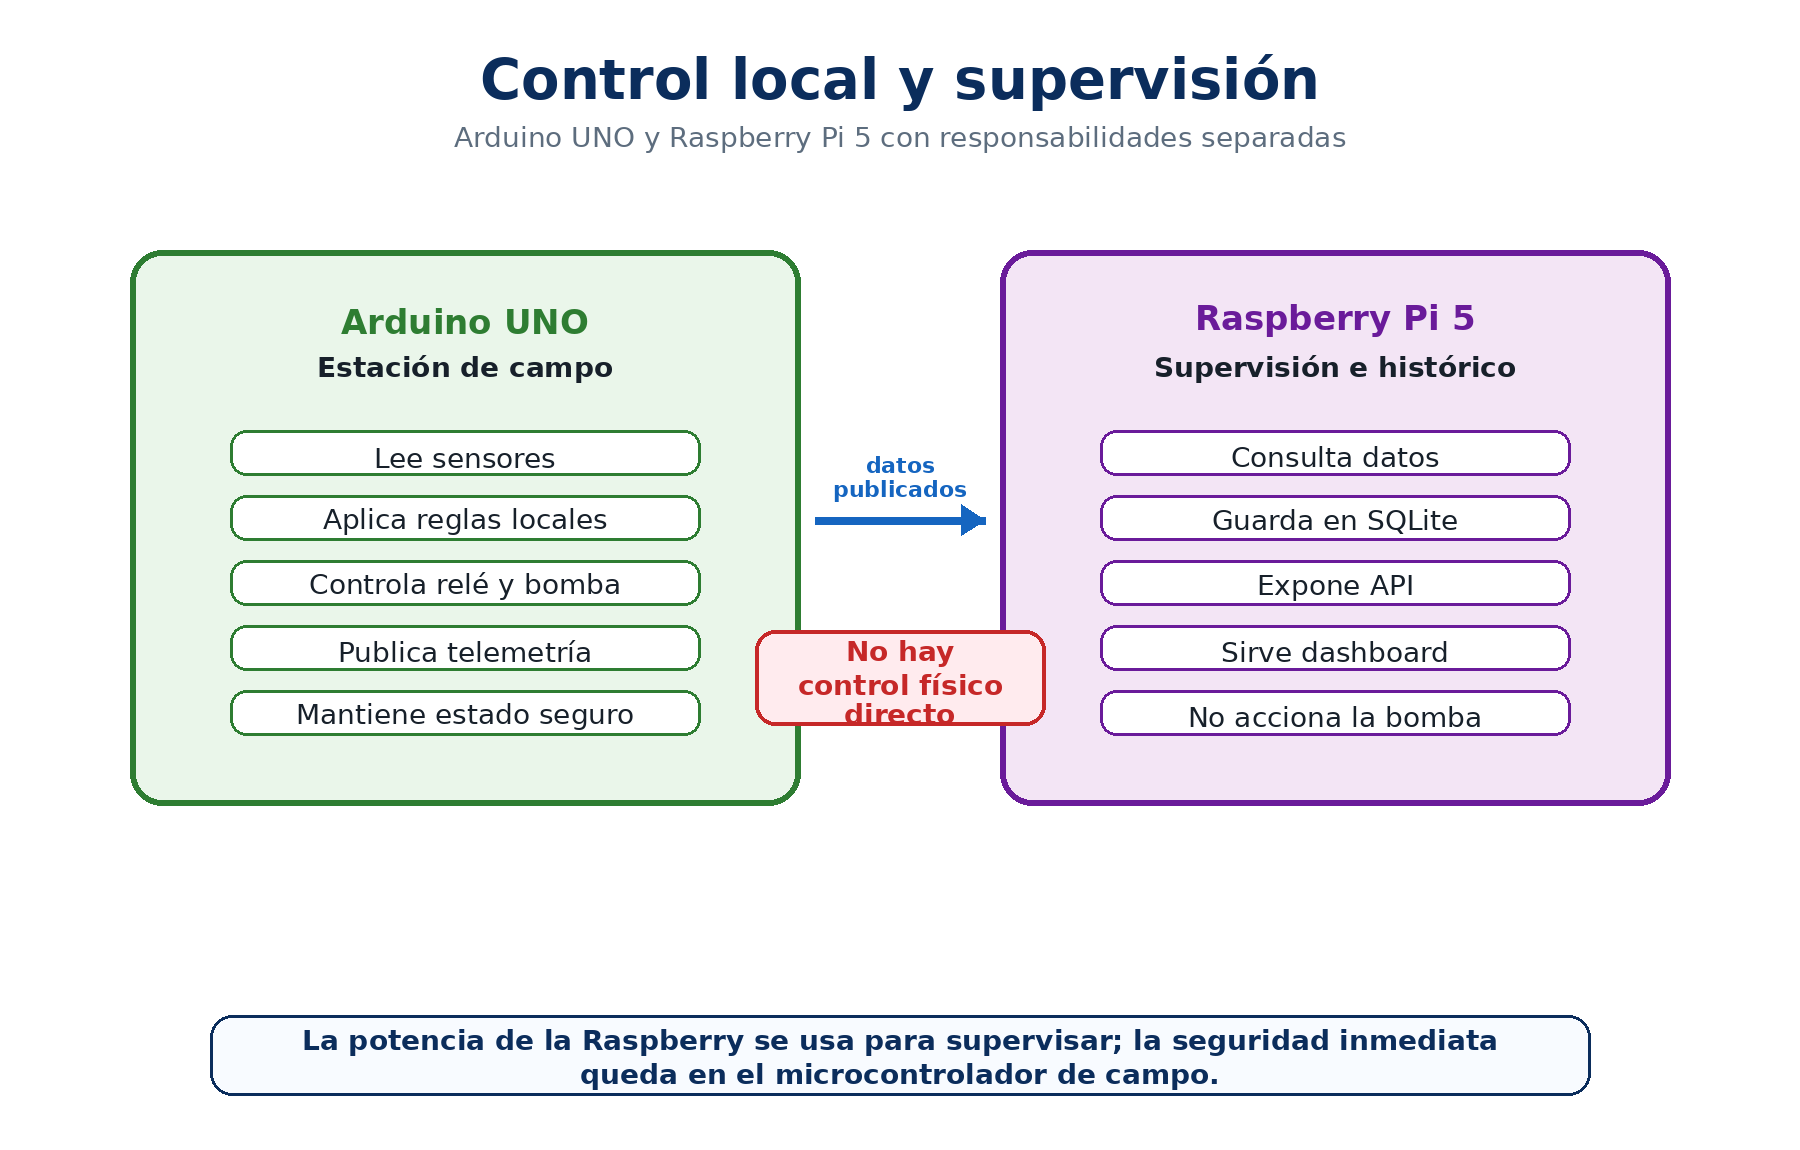
\includegraphics[width=\textwidth]{figs/figura_3_7_plataformas_control_supervision.png}
    \caption{Separación de responsabilidades entre Arduino UNO y Raspberry Pi 5.}
    \label{fig:cap3_plataformas_control_supervision}
\end{figure}

Arduino UNO se ha seleccionado como plataforma principal de las estaciones de campo porque ofrece una integración directa con sensores, bus I2C, entrada analógica, comunicación serie con el módem LTE y control digital del relé. Sus prestaciones son limitadas frente a plataformas más modernas, pero suficientes para las tareas previstas en el nodo de campo: medir, aplicar reglas locales, comunicarse y actuar sobre la bomba \cite{arduino_uno_rev3_specs}.

La Raspberry Pi 5 se utiliza como sistema de supervisión, no como controlador físico del riego. Su mayor capacidad permite ejecutar procesos software, mantener una base de datos local, servir una API y alojar el dashboard web \cite{raspberry_pi5_product_brief}. Esta separación evita concentrar en un único dispositivo tareas muy distintas y permite que la estación mantenga un comportamiento seguro aunque la Raspberry no esté disponible.

La Tabla~\ref{cuadro:arduino_raspberry_tierraviva} resume esta división de responsabilidades.

\begin{table}[H]
\begin{center}
\small
\renewcommand{\arraystretch}{1.15}
\rowcolors{2}{TableRowSoft}{white}

\begin{tabular}{|p{0.24\textwidth}|p{0.32\textwidth}|p{0.32\textwidth}|}
\hline
\rowcolor{URJCRed}
\TVHead{Aspecto} & \TVHead{Arduino UNO} & \TVHead{Raspberry Pi 5} \\
\hline
Rol en TierraViva & Controlador local autónomo de estación de campo. & Sistema de supervisión, almacenamiento y visualización. \\
\hline
Relación con sensores & Lectura directa de sensores analógicos y digitales. & No lee sensores directamente en la arquitectura final. \\
\hline
Actuación & Decisión local y control del relé asociado a la bomba. & No participa en la actuación física ni genera órdenes de riego. \\
\hline
Capacidad software & Firmware sencillo y tareas embebidas. & Sistema operativo, API, base de datos y dashboard. \\
\hline
Consumo y arranque & Menor consumo y arranque inmediato. & Mayor consumo y arranque dependiente del sistema operativo. \\
\hline
Adecuación principal & Nodo de campo sencillo y robusto. & Procesamiento, histórico y supervisión. \\
\hline
\end{tabular}
\caption{Comparación funcional entre Arduino UNO y Raspberry Pi 5 en TierraViva}
\label{cuadro:arduino_raspberry_tierraviva}
\end{center}
\end{table}

Durante el diseño también se consideraron alternativas como ESP32 o STM32. ESP32 habría aportado mayor potencia y conectividad integrada, pero en TierraViva la comunicación remota se resuelve mediante un módem LTE externo. STM32 ofrece más prestaciones, aunque aumenta la complejidad de configuración y depuración. Para el alcance del TFG, la combinación Arduino UNO y Raspberry Pi 5 mantiene un equilibrio adecuado entre sencillez, coste, capacidad técnica y reproducibilidad.

\section{Selección de solución de comunicaciones para estaciones remotas}
\label{sec:seleccion_comunicaciones_remotas}

La comunicación entre las estaciones de campo y el sistema de supervisión es una decisión crítica en TierraViva. Las estaciones no se consideran conectadas físicamente a la Raspberry Pi, por lo que la telemetría debe enviarse de forma remota desde la parcela o zona de cultivo. La solución elegida debía funcionar sin depender de una red WiFi local, permitir integración con una plataforma cloud y ser verificable dentro del alcance temporal del TFG.

Durante el diseño se valoraron principalmente dos enfoques: LoRa/LoRaWAN y conectividad móvil LTE. LoRa resulta especialmente atractivo en IoT agrícola por su largo alcance, bajo consumo y adecuación a mensajes pequeños \cite{semtech2015lora_modulation,augustin2016lora}. LoRaWAN añade una arquitectura de red con dispositivos finales, pasarelas y servidores de red \cite{lora_alliance_104}. Sin embargo, esta opción habría requerido resolver infraestructura adicional, selección de módulos, compatibilidad de banda, alimentación, niveles lógicos y configuración de red, desplazando una parte importante del esfuerzo hacia la propia comunicación.

LTE con el módulo A7670E-LASA se eligió como alternativa más adecuada para validar el sistema completo. Esta opción permite que cada estación publique datos directamente en Internet mediante red móvil y peticiones HTTP, sin desplegar gateway propio. A cambio, introduce dependencia de cobertura móvil, tarjeta SIM, consumo energético superior y una alimentación más exigente para el módem.

\begin{table}[H]
\begin{center}
\small
\renewcommand{\arraystretch}{1.15}
\rowcolors{2}{TableRowSoft}{white}

\begin{tabular}{|p{0.24\textwidth}|p{0.30\textwidth}|p{0.34\textwidth}|}
\hline
\rowcolor{URJCRed}
\TVHead{Criterio} & \TVHead{LoRa/LoRaWAN} & \TVHead{LTE con A7670E-LASA} \\
\hline
Alcance & Muy adecuado para largas distancias con baja tasa de datos. & Depende de la cobertura de red móvil disponible. \\
\hline
Consumo & Bajo consumo, especialmente en envíos periódicos. & Mayor consumo y picos de corriente durante transmisión. \\
\hline
Infraestructura & Puede requerir gateway, servidor LoRaWAN o receptor propio. & No requiere gateway propio; usa red móvil existente. \\
\hline
Integración cloud & Necesita pasarela o backend intermedio. & Integración directa mediante HTTP. \\
\hline
Complejidad inicial & Mayor si se despliega LoRaWAN completo. & Menor para validar telemetría HTTP. \\
\hline
Coste operativo & Sin SIM ni tarifa de datos si la red es propia. & Requiere tarjeta SIM y servicio de datos. \\
\hline
Riesgo para el TFG & Riesgo de consumir mucho tiempo en la red. & Riesgo menor para obtener un prototipo funcional completo. \\
\hline
Adecuación al prototipo & Muy interesante como línea futura o alternativa avanzada. & Adecuada para validar el sistema completo en el alcance actual. \\
\hline
\end{tabular}
\caption{Comparación entre LoRa/LoRaWAN y LTE para TierraViva}
\label{cuadro:comparacion_lora_lte_tierraviva}
\end{center}
\end{table}

La decisión final no implica que LoRa/LoRaWAN sea tecnológicamente inferior. De hecho, puede ser una línea futura adecuada para versiones orientadas a bajo consumo y despliegues con infraestructura propia. En este TFG se prioriza una solución funcional, verificable y defendible, capaz de completar el flujo de medida, publicación, almacenamiento, visualización y actuación local. La validación técnica del A7670E-LASA mediante comandos AT y su integración con Arduino se desarrolla en el Capítulo~\ref{cap:implementacion_hardware_firmware}.

\section{Elección de plataforma cloud: ThingSpeak}
\label{sec:eleccion_plataforma_cloud}

La plataforma cloud debía actuar como capa intermedia entre las estaciones remotas y la Raspberry Pi. Su función principal no es decidir el riego, sino permitir que las estaciones publiquen telemetría y que el sistema de supervisión pueda consultar esos datos sin conexión física con los nodos de campo.

Se valoraron alternativas como brokers MQTT accesibles desde Internet, Ubidots, Adafruit IO, Blynk, ThingsBoard o una plataforma propia. Sin embargo, para el alcance del TFG se buscaba una solución sencilla, verificable y compatible con dispositivos embebidos. ThingSpeak se seleccionó porque ofrece una estructura basada en canales y campos, permite escribir datos mediante API HTTP y facilita una primera visualización de las medidas publicadas \cite{thingspeak_docs,thingspeak_write_data}.

\begin{figure}[H]
    \centering
    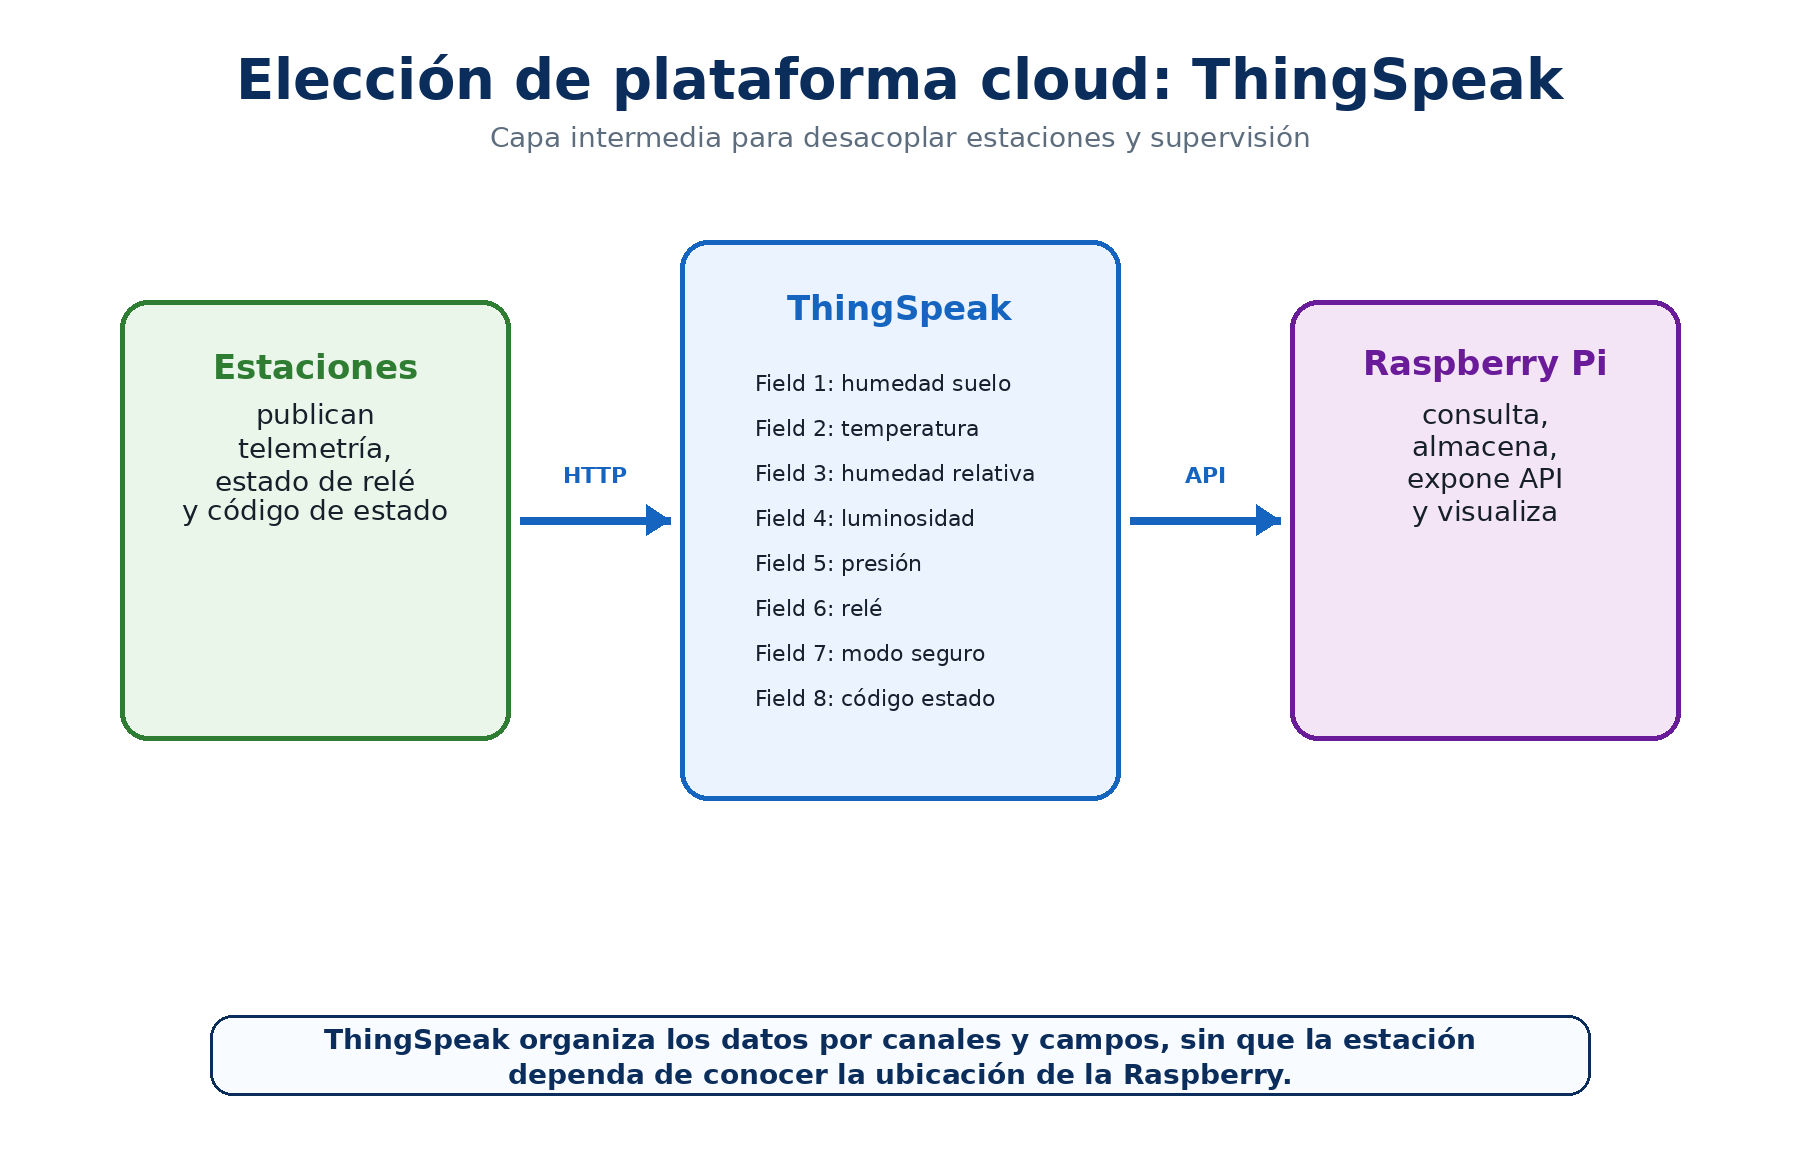
\includegraphics[width=0.78\textwidth]{figs/figura_3_9_thingspeak_capa_intermedia.png}
    \caption{Uso de ThingSpeak como capa intermedia entre estaciones remotas y sistema de supervisión. La plataforma organiza la telemetría y los estados por canales y campos, permitiendo su consulta posterior desde Raspberry Pi.}
    \label{fig:cap3_thingspeak_capa_intermedia}
\end{figure}

En TierraViva se utilizan canales diferenciados para cada estación, lo que permite separar los datos de TierraViva\_A y TierraViva\_B. Cada publicación contiene medidas ambientales, estado del relé, evento de sistema y código auxiliar de diagnóstico. Esta organización facilita la trazabilidad, evita mezclar lecturas de distintas estaciones y permite que la Raspberry Pi consulte los datos de forma independiente.

ThingSpeak presenta limitaciones que deben asumirse. No es una plataforma de tiempo real estricto y su uso introduce dependencia de conectividad, latencia y disponibilidad del servicio. Sin embargo, estas limitaciones no comprometen la actuación física del riego, ya que la decisión crítica se ejecuta localmente en cada estación. La nube se reserva para telemetría, histórico, supervisión y diagnóstico.

La estructura concreta de canales, campos y códigos publicados se desarrolla en el Capítulo~\ref{cap:capitulo4} y en el Anexo~\ref{anexo:estructura_thingspeak_estados}. La lectura de datos desde Raspberry Pi se explica en el Capítulo~\ref{cap:implementacion_software_raspberry_nube}.

\section{Elección de arquitectura software de supervisión en Raspberry Pi}
\label{sec:eleccion_arquitectura_software_raspberry}

La Raspberry Pi se ha seleccionado como sistema de supervisión software de TierraViva. Su función no es sustituir a las estaciones de campo, leer directamente los sensores ni decidir la activación de la bomba, sino consultar la información publicada por las estaciones, registrar un histórico local y ofrecer una interfaz de consulta. Esta separación resulta importante porque las estaciones se encuentran en campo y se comunican de forma remota, mientras que la Raspberry actúa como nodo de supervisión e histórico.

\begin{figure}[H]
    \centering
    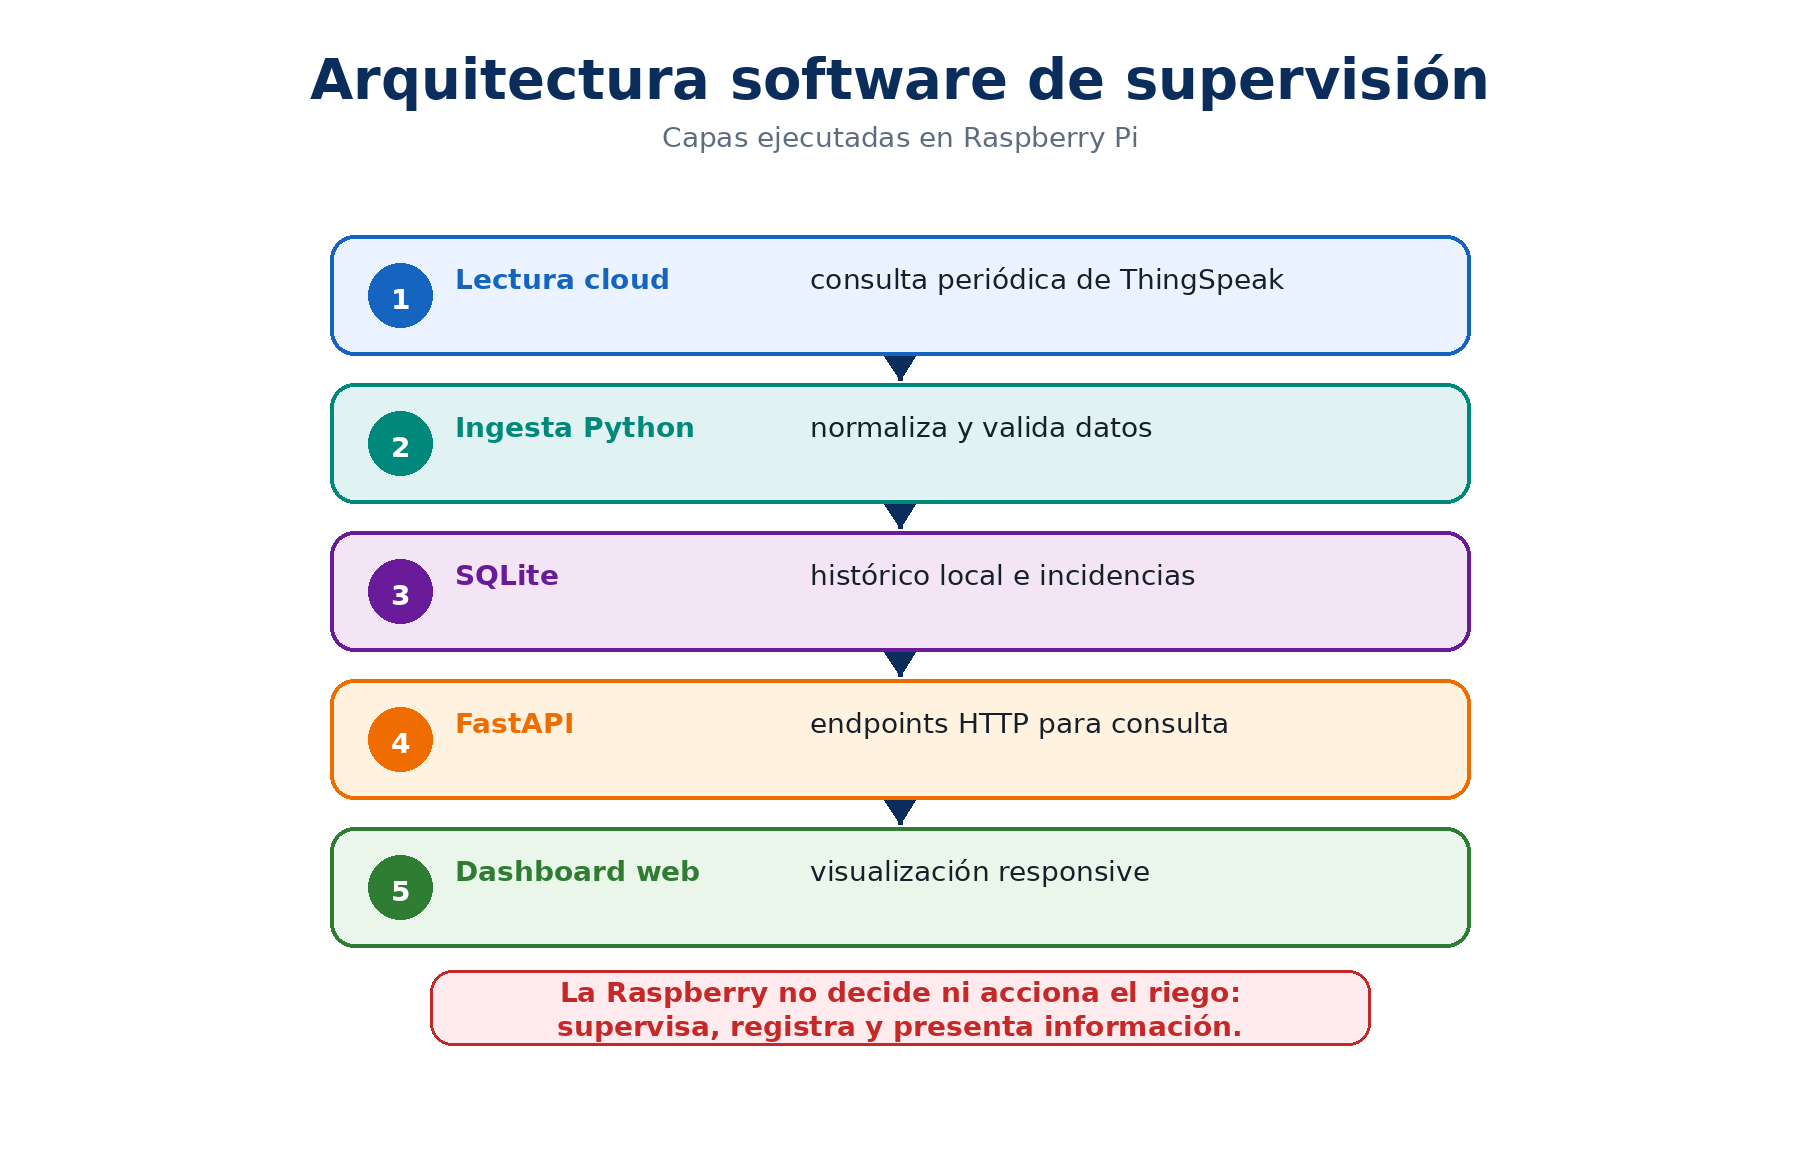
\includegraphics[width=\textwidth]{figs/figura_3_10_arquitectura_software_raspberry.png}
    \caption{Arquitectura software de supervisión en Raspberry Pi. La información publicada en la nube se consulta, valida, almacena en SQLite, expone mediante FastAPI y se presenta en el dashboard web.}
    \label{fig:cap3_arquitectura_software_raspberry}
\end{figure}

La arquitectura software de supervisión se apoya en tres bloques principales: almacenamiento local, API y dashboard. SQLite se selecciona como base de datos local por su sencillez de despliegue y por ser suficiente para conservar el histórico de lecturas, estados e incidencias del prototipo sin instalar un servidor de base de datos adicional \cite{sqlite_about}. Esta decisión permite que la Raspberry Pi mantenga una memoria propia del sistema, complementaria a los datos publicados en ThingSpeak.

FastAPI se selecciona como framework para construir la API de supervisión en Python \cite{fastapi_docs}. Su papel dentro de TierraViva es actuar como capa intermedia entre la base de datos y la interfaz web, evitando que el dashboard acceda directamente a SQLite o a los detalles internos de almacenamiento. La API permite consultar datos mediante peticiones HTTP y deja preparada la arquitectura para que otros clientes puedan reutilizar la misma información en futuras ampliaciones.

El dashboard web constituye la capa de presentación del sistema. Su objetivo es mostrar de forma comprensible las últimas lecturas, el estado de las estaciones y la información operativa publicada por cada nodo. De esta manera, la Raspberry Pi no se limita a almacenar datos, sino que los transforma en información útil para supervisar el comportamiento del prototipo.

La implementación concreta de estos bloques, incluyendo la estructura de los scripts, los endpoints expuestos, el modelo de datos y la evolución desde el prototipo local previo, se desarrolla en el Capítulo~\ref{cap:implementacion_software_raspberry_nube}.

\begin{table}[H]
\begin{center}
\small
\renewcommand{\arraystretch}{1.15}
\rowcolors{2}{TableRowSoft}{white}

\begin{tabular}{|p{0.25\textwidth}|p{0.34\textwidth}|p{0.29\textwidth}|}
\hline
\rowcolor{URJCRed}
\TVHead{Bloque software} & \TVHead{Función en TierraViva} & \TVHead{Motivo de elección} \\
\hline
Prototipo MQTT local & Validación previa de la cadena software en Raspberry. & Permitió comprobar recepción, almacenamiento, API y visualización antes de adoptar la arquitectura final con ThingSpeak. \\
\hline
Ingesta desde ThingSpeak & Consulta periódica de telemetría y estado publicados por las estaciones. & Permite alimentar el histórico local y el dashboard sin conexión directa con los nodos de campo. \\
\hline
SQLite & Almacenamiento local de lecturas, estados e incidencias. & Base de datos ligera, autocontenida y suficiente para el prototipo. \\
\hline
FastAPI & Exposición de datos mediante endpoints HTTP. & Facilita crear una API sencilla entre la base de datos y el dashboard. \\
\hline
Dashboard web & Visualización de medidas, histórico, estado del relé y estado de las estaciones. & Permite supervisar el prototipo sin acceder a consola o consultas SQL. \\
\hline
\end{tabular}
\caption{Bloques principales de la arquitectura software de supervisión en Raspberry Pi}
\label{cuadro:arquitectura_software_raspberry}
\end{center}
\end{table}

La lógica de decisión de riego no se mantiene en la Raspberry Pi en la arquitectura final. Aunque este dispositivo tiene capacidad suficiente para aplicar reglas más complejas, se ha decidido desplazar la decisión crítica al nodo de campo. Esta elección reduce la dependencia de la red y evita que la actuación física dependa de un comando remoto.

La Raspberry conserva un papel relevante como sistema de supervisión: consulta los datos publicados, mantiene un histórico local, expone la API y sirve el dashboard. La implementación concreta de estos bloques se desarrolla en el Capítulo~\ref{cap:implementacion_software_raspberry_nube}. La referencia de endpoints se recoge en el Anexo~\ref{anexo:manual_api}, y el uso de la interfaz por parte del usuario se documenta en el Anexo~\ref{anexo:manual_usuario}.

\section{Materiales empleados}
\label{sec:materiales_empleados}

La selección de materiales se ha realizado buscando un equilibrio entre funcionalidad, coste, disponibilidad y facilidad de integración. Al tratarse de un prototipo de TFG, se han utilizado módulos habituales en sistemas IoT y prototipos electrónicos, evitando componentes industriales cerrados que aumentarían el coste y dificultarían la reproducción del montaje.

Desde el punto de vista funcional, el sistema se organiza en bloques de sensórica, control local, comunicación, supervisión, actuación y alimentación. La sensórica se basa en un sensor capacitivo de humedad de suelo, BME280 y BH1750/GY-302; el control local se realiza con Arduino UNO; la comunicación remota con A7670E-LASA y tarjeta SIM; la supervisión con Raspberry Pi 5; y la actuación mediante relé y bomba de agua de 12 V.

El inventario completo, las referencias comerciales, cantidades, precios, imágenes y observaciones de compra se recogen en el Anexo~\ref{anexo:materiales}. El conexionado eléctrico se documenta en el Anexo~\ref{anexo:esquemas_electricos}, y la validación asociada a sensores, comunicación, actuación y flujo extremo a extremo se desarrolla en los Anexos~\ref{anexo:plan_pruebas} y \ref{anexo:trazabilidad_requisitos_pruebas}.

\section{Riesgos técnicos y medidas de mitigación}
\label{sec:riesgos_tecnicos_mitigacion}

El diseño de TierraViva debe contemplar fallos de sensores, alimentación, comunicación, software y actuación. Esta consideración es especialmente importante porque el prototipo no se limita a monitorizar variables ambientales, sino que acciona físicamente una bomba de agua. Por ello, el criterio general adoptado es conservador: ante una lectura inválida, una condición no verificable o un fallo relevante, la estación debe mantener la bomba apagada.

La Tabla~\ref{cuadro:riesgos_mitigacion} resume los riesgos técnicos principales considerados durante el diseño. El análisis completo de probabilidad, impacto, criticidad, riesgo residual y pruebas asociadas se desarrolla en el Anexo~\ref{anexo:gestion_riesgos}.

\begin{table}[H]
\begin{center}
\small
\renewcommand{\arraystretch}{1.15}
\rowcolors{2}{TableRowSoft}{white}

\begin{tabular}{|p{0.24\textwidth}|p{0.30\textwidth}|p{0.34\textwidth}|}
\hline
\rowcolor{URJCRed}
\TVHead{Riesgo} & \TVHead{Impacto posible} & \TVHead{Medida de mitigación} \\
\hline
Fallo de alimentación o picos de consumo & Reinicios, pérdida de comunicación o comportamiento inestable del relé. & Regulación con LM2596, comprobación de tensiones, masa común y condensadores de estabilización. \\
\hline
Lecturas erróneas o inestables & Decisiones de riego basadas en datos no fiables. & Validación de rangos, descarte de valores incoherentes, pruebas por bloques y calibración progresiva. \\
\hline
Regla local mal configurada & Activación del riego en condiciones no deseadas. & Umbrales configurables, cooldown, pruebas controladas y actuación limitada por firmware. \\
\hline
Activación prolongada de la bomba & Riego indefinido o consumo innecesario de agua. & Bomba apagada por defecto, tiempo máximo de actuación y apagado explícito al finalizar el riego. \\
\hline
Pérdida de comunicación & Ausencia de telemetría o supervisión remota incompleta. & Decisión local independiente, publicación de estados cuando sea posible y supervisión de datos obsoletos. \\
\hline
Fallo del software en Raspberry Pi & Pérdida temporal de API, dashboard o histórico local. & Separación por módulos, logs, script de gestión y autonomía de las estaciones para la decisión de riego. \\
\hline
\end{tabular}
\caption{Resumen de riesgos técnicos principales y medidas de mitigación}
\label{cuadro:riesgos_mitigacion}
\end{center}
\end{table}

Estas medidas siguen un principio común: separar supervisión y control local. La Raspberry Pi permite registrar, consultar y visualizar el estado del sistema, pero la seguridad de la actuación reside en la estación de campo. De este modo, una caída del dashboard, una pérdida de comunicación o un dato no fiable no deben provocar una activación no controlada de la bomba.

El desarrollo completo de esta gestión de riesgos se recoge en el Anexo~\ref{anexo:gestion_riesgos}. La relación entre riesgos, requisitos y pruebas se documenta además en el Anexo~\ref{anexo:trazabilidad_requisitos_pruebas}.


\chapter{Arquitectura final de TierraViva}
\label{cap:capitulo4}

Una vez definidos los requisitos, los materiales y las principales decisiones de diseño, este capítulo presenta la arquitectura final de TierraViva. A diferencia del capítulo anterior, donde se justifican las alternativas valoradas y los criterios de elección, aquí se describe cómo queda organizado el sistema completo y cómo interactúan sus distintos bloques durante el funcionamiento.

La arquitectura final se basa en estaciones de campo autónomas con Arduino UNO, sensores ambientales y de suelo, comunicación LTE mediante el módulo A7670E-LASA, una plataforma cloud intermedia basada en ThingSpeak y un sistema de supervisión implementado sobre Raspberry Pi 5. El sistema se ha diseñado para cubrir el ciclo completo de monitorización y actuación local: adquisición de datos, decisión de riego en la estación, actuación sobre la bomba, publicación de telemetría y estado, almacenamiento histórico, API y visualización mediante dashboard web.

El cambio principal respecto a planteamientos anteriores es que la Raspberry Pi no actúa como elemento central de decisión del riego. La decisión crítica se desplaza al firmware de cada estación, que evalúa sus propias lecturas y aplica reglas locales de seguridad. La Raspberry conserva un papel importante, pero orientado a supervisión, histórico y visualización.

\section{Visión general de la arquitectura}
\label{sec:vision_general_arquitectura}

La arquitectura final de TierraViva se organiza como un sistema IoT distribuido. Las medidas se obtienen en campo, la comunicación se realiza mediante red móvil, la información se publica en una plataforma cloud y la supervisión se ejecuta desde una Raspberry Pi 5. La actuación sobre el riego, sin embargo, no depende de una decisión externa enviada desde la Raspberry, sino de reglas locales ejecutadas en cada estación.

El sistema está formado por cuatro elementos principales: las estaciones autónomas de campo A y B, la plataforma ThingSpeak, la Raspberry Pi 5 y el dashboard web. Las estaciones se encargan de medir, decidir y actuar localmente. ThingSpeak funciona como capa intermedia de telemetría y estado. La Raspberry Pi consulta los datos, mantiene un histórico local y expone una API. El dashboard permite supervisar el estado del sistema desde una interfaz web.

La Figura~\ref{fig:arquitectura_final_tierraviva} muestra la arquitectura final del sistema.

\begin{figure}[H]
\centering
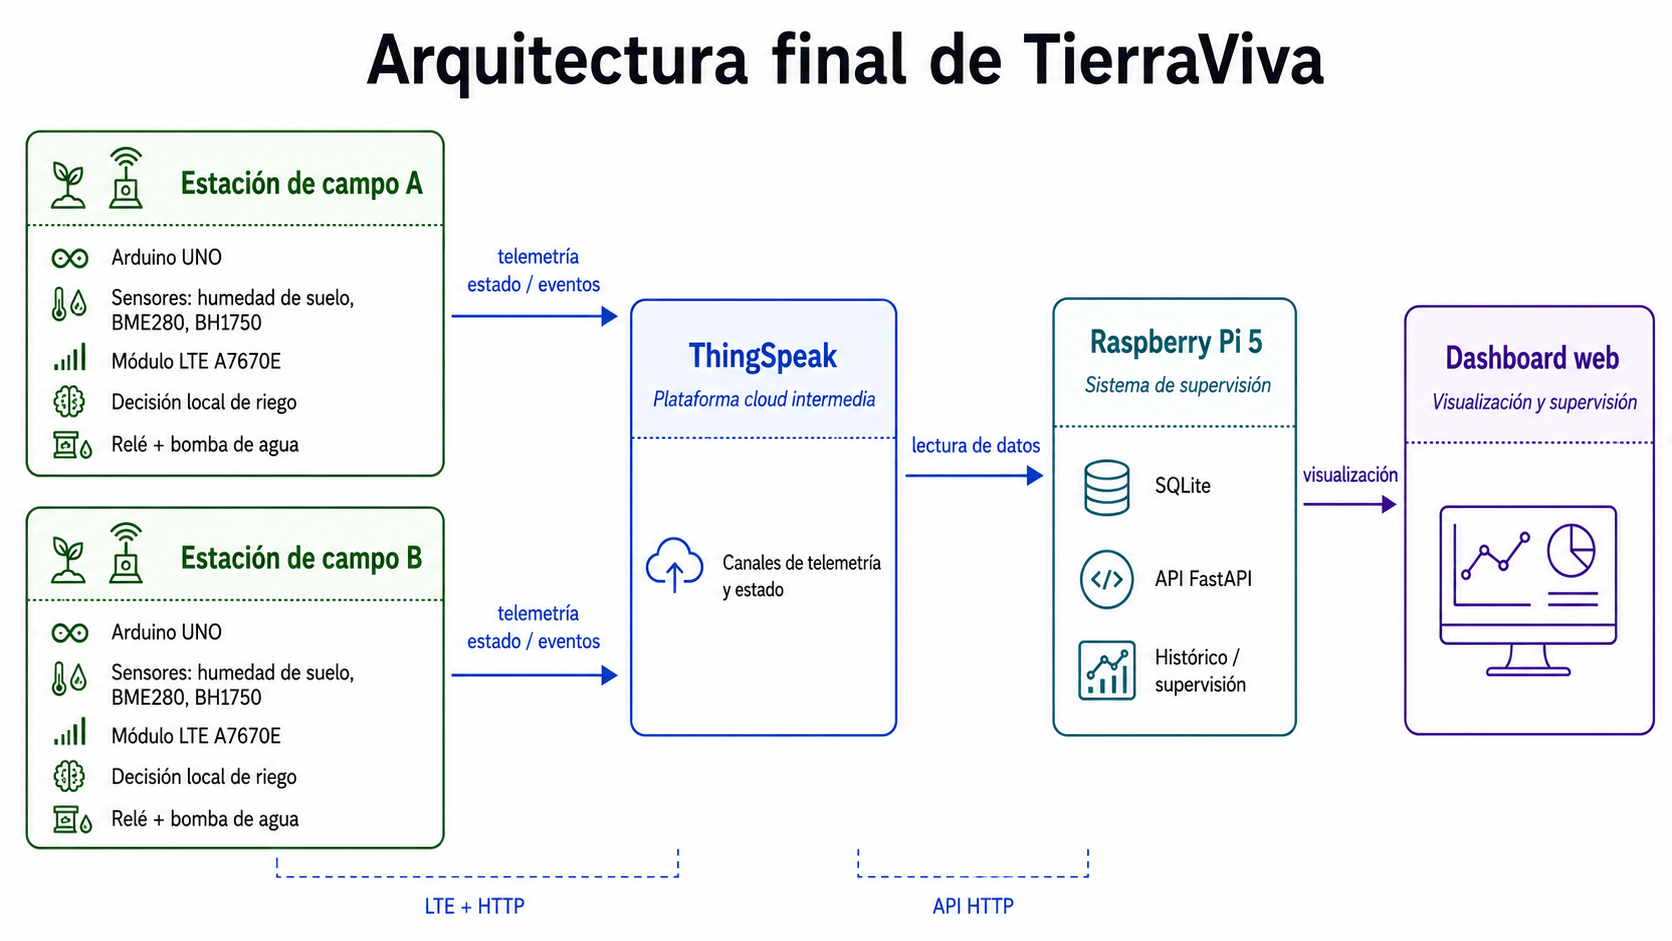
\includegraphics[width=\textwidth]{figs/arquitecturaFinalTierraViva.png}
\caption{Arquitectura final de TierraViva con decisión local en las estaciones.}
\label{fig:arquitectura_final_tierraviva}
\end{figure}

El flujo de funcionamiento comienza en las estaciones de campo. Cada estación toma lecturas de sus sensores, evalúa localmente si se cumplen las condiciones de riego y, si procede, activa la bomba de agua mediante el relé durante un tiempo limitado. Después publica en ThingSpeak tanto las medidas ambientales como el estado del relé y el código de estado correspondiente.

ThingSpeak actúa como punto de desacoplo entre los nodos de campo y el sistema de supervisión. Las estaciones no necesitan conocer la ubicación de la Raspberry ni mantener una conexión directa con ella; únicamente publican información en la nube. La Raspberry, por su parte, consulta periódicamente los canales de ThingSpeak y almacena los datos relevantes en su base de datos local.

La Raspberry Pi 5 funciona como sistema de supervisión. Su papel no es accionar directamente la bomba, leer sensores por cable ni decidir cuándo debe regarse. Su función es consultar la telemetría disponible, registrar el histórico en SQLite, exponer los datos mediante una API y servir el dashboard web. Así, una caída de la Raspberry no impide que la estación mantenga su comportamiento local de seguridad.

El dashboard web representa la capa de visualización. A partir de la información procesada por la Raspberry Pi, permite consultar las últimas lecturas, el estado de las estaciones, el estado del relé y los estados de funcionamiento publicados por cada nodo. No participa directamente en la actuación, pero resulta fundamental para supervisar el comportamiento del prototipo y detectar posibles incidencias.

La arquitectura final puede resumirse de forma sencilla: las estaciones miden, deciden y actúan en campo; ThingSpeak comunica y almacena telemetría; la Raspberry registra y supervisa; y el dashboard permite visualizar. Esta organización facilita la validación por bloques, permite trabajar con más de una estación y mantiene una separación clara entre adquisición, comunicación, decisión local, actuación y supervisión.

\section{Estaciones de campo A y B}
\label{sec:estaciones_campo_ab}

Las estaciones de campo son los nodos autónomos de TierraViva. Su función dentro de la arquitectura final es adquirir datos del entorno, evaluar localmente reglas de riego, accionar la bomba cuando corresponda y publicar telemetría y estado en la plataforma cloud. En esta versión del sistema se contemplan dos estaciones, denominadas estación A y estación B, con una estructura hardware equivalente y una configuración lógica diferenciada.

Ambas estaciones siguen el mismo diseño base: Arduino UNO como controlador local, sensores de suelo y ambientales, módulo LTE A7670E-LASA para comunicación remota, relé para accionar la bomba de agua y alimentación principal a 12 V con regulación a 5 V mediante LM2596. La diferencia entre ellas no está en la arquitectura física, sino en el identificador de estación y el canal de ThingSpeak utilizado para publicar sus datos.

\begin{table}[H]
\begin{center}
\small
\begin{tabular}{|p{0.26\textwidth}|p{0.30\textwidth}|p{0.34\textwidth}|}
\hline
\textbf{Elemento} & \textbf{Estación A} & \textbf{Estación B} \\
\hline
Identificador lógico & \texttt{TierraViva\_A} & \texttt{TierraViva\_B} \\
\hline
Controlador local & Arduino UNO & Arduino UNO \\
\hline
Sensores & Humedad de suelo, BME280 y BH1750 & Humedad de suelo, BME280 y BH1750 \\
\hline
Comunicación & A7670E-LASA mediante LTE/HTTP & A7670E-LASA mediante LTE/HTTP \\
\hline
Canal ThingSpeak & Canal asociado a estación A & Canal asociado a estación B \\
\hline
Decisión de riego & Regla local en firmware & Regla local en firmware \\
\hline
Actuación & Relé y bomba de agua 12 V & Relé y bomba de agua 12 V \\
\hline
Alimentación & 12 V con regulación a 5 V & 12 V con regulación a 5 V \\
\hline
\end{tabular}
\caption{Configuración lógica de las estaciones de campo}
\label{cuadro:configuracion_estaciones}
\end{center}
\end{table}

La Tabla~\ref{cuadro:configuracion_estaciones} resume esta configuración. El objetivo de mantener estaciones equivalentes es facilitar la reproducción del sistema: una vez validada la estación A, la estación B puede construirse replicando el mismo montaje y modificando únicamente los parámetros de identificación y comunicación. Esta decisión también simplifica la depuración, ya que cualquier diferencia de comportamiento entre estaciones puede analizarse a partir de una base hardware común.

Desde el punto de vista interno, cada estación se organiza en cuatro bloques funcionales. El primero es el bloque de adquisición, formado por el sensor capacitivo de humedad del suelo, el BME280 y el BH1750. El segundo es el bloque de decisión local, ejecutado en el firmware del Arduino. El tercero es el bloque de comunicación, formado por el A7670E-LASA y la lógica de publicación mediante HTTP. El cuarto es el bloque de actuación, formado por la salida digital del Arduino, el módulo relé y la bomba de agua de 12 V.

\begin{table}[H]
\begin{center}
\small
\begin{tabular}{|p{0.25\textwidth}|p{0.32\textwidth}|p{0.33\textwidth}|}
\hline
\textbf{Bloque interno} & \textbf{Elementos implicados} & \textbf{Responsabilidad} \\
\hline
Adquisición & Sensores y Arduino UNO & Obtener lecturas periódicas del suelo y del entorno. \\
\hline
Decisión local & Arduino UNO & Evaluar humedad del suelo, cooldown, errores y condiciones de seguridad. \\
\hline
Comunicación & Arduino UNO y A7670E-LASA & Publicar telemetría, estado y eventos en ThingSpeak. \\
\hline
Actuación & Arduino UNO, relé y bomba & Ejecutar el riego localmente durante un tiempo limitado. \\
\hline
Alimentación & Fuente 12 V, LM2596 y condensadores & Proporcionar tensión adecuada y estabilidad eléctrica al montaje. \\
\hline
\end{tabular}
\caption{Bloques internos de una estación de campo}
\label{cuadro:bloques_internos_estacion}
\end{center}
\end{table}

El firmware de estación debe mantener esta separación de responsabilidades. En primer lugar, realiza la lectura de sensores y genera una estructura de datos con las variables medidas. Después, comprueba si las lecturas son válidas y evalúa la regla local de riego. Si la humedad del suelo indica sequedad, no existe cooldown activo y no se detecta una condición de error, la estación puede activar el relé durante el tiempo máximo configurado.

La actuación se ejecuta siempre de forma local. Cuando una estación decide regar, activa el relé durante un tiempo limitado y posteriormente vuelve a dejar la bomba apagada. Durante las pruebas iniciales puede utilizarse una carga de baja potencia, como un LED, para comprobar la lógica de activación sin accionar todavía la bomba real. En el montaje final, esa carga de prueba se sustituye por la bomba de agua de 12 V.

La estación conserva la responsabilidad última sobre la ejecución segura. Antes de activar el relé debe comprobar que la lectura de humedad es válida, que la duración máxima no se supera, que no existe un error crítico y que no se está dentro del periodo mínimo entre riegos. Si alguna de estas comprobaciones falla, la estación mantiene la bomba apagada y publica un código de estado que permita diagnosticar la situación desde la Raspberry Pi.

La alimentación de cada estación parte de una tensión principal de 12 V, necesaria para el bloque de actuación. A partir de esa tensión se obtiene una línea de 5 V mediante el regulador LM2596 para alimentar la electrónica compatible. En el montaje se incorporan condensadores de estabilización para reducir inestabilidades asociadas a consumos variables, especialmente durante la comunicación LTE o los cambios de estado del bloque de actuación. El detalle de conexiones eléctricas se recoge en el Anexo~\ref{anexo:esquemas_conexion}.

En resumen, las estaciones A y B son nodos de campo equivalentes desde el punto de vista hardware, pero diferenciados por configuración. Esta organización permite escalar el sistema sin rediseñar la arquitectura: añadir una nueva estación implicaría replicar el montaje, asignar un nuevo identificador, crear un nuevo canal de ThingSpeak y ajustar la lógica de supervisión para consultar ese nuevo origen de datos.

\section{Arquitectura de comunicaciones LTE/HTTP}
\label{sec:arquitectura_comunicaciones_lte_http}

La comunicación de las estaciones de campo se basa en el módulo LTE A7670E-LASA y en el uso de peticiones HTTP hacia ThingSpeak. Esta arquitectura permite que cada estación publique telemetría y estado desde una ubicación remota sin depender de una red WiFi local ni de una conexión física con la Raspberry Pi. Desde el punto de vista funcional, el módulo LTE actúa como interfaz de salida a Internet de la estación.

El Arduino UNO no accede directamente a la red móvil. Su papel es comunicarse por UART con el A7670E-LASA mediante comandos AT. A través de esa interfaz serie, el firmware comprueba el estado del módulo, verifica la SIM, confirma el registro en red, configura el contexto de datos y lanza las peticiones HTTP necesarias para enviar información a la nube. Esta separación permite que el Arduino mantenga una lógica relativamente sencilla: preparar datos, aplicar la decisión local, enviarlos al módem y analizar la respuesta obtenida.

El flujo de comunicación se organiza en varias fases. La primera corresponde a la inicialización del módulo. En esta fase, la estación comprueba que el A7670E-LASA responde a comandos básicos y que la comunicación serie funciona correctamente. Después, se verifica el estado de la SIM y el registro en la red móvil. Una estación no debería intentar enviar telemetría si el módulo no responde, si la SIM no está preparada o si no existe registro válido en red.

A continuación, se configura el contexto de datos. Para ello, el módulo debe disponer de un APN válido asociado a la tarjeta SIM utilizada. Este paso es necesario para que el módem pueda obtener conectividad IP. Una vez configurado el contexto y obtenida una dirección IP, la estación puede iniciar la secuencia HTTP.

La fase de envío consiste en construir una URL de actualización de ThingSpeak con los campos de telemetría correspondientes. Cada estación incluye sus medidas y estados en los campos definidos para su canal: humedad de suelo, temperatura, humedad relativa, luminosidad, presión, estado del relé, código de estado o evento y un campo auxiliar de diagnóstico. El A7670E-LASA realiza entonces una petición HTTP hacia la API de ThingSpeak.

\begin{table}[H]
\begin{center}
\small
\begin{tabular}{|p{0.22\textwidth}|p{0.31\textwidth}|p{0.35\textwidth}|}
\hline
\textbf{Fase} & \textbf{Acción principal} & \textbf{Resultado esperado} \\
\hline
Inicialización & Comprobar comunicación con el módulo mediante comandos AT. & El módulo responde correctamente y queda listo para continuar. \\
\hline
SIM & Verificar que la tarjeta SIM está disponible y sin PIN pendiente. & La SIM se encuentra preparada para registrarse en red. \\
\hline
Registro en red & Comprobar el registro LTE y la calidad de señal. & La estación confirma que existe cobertura móvil suficiente. \\
\hline
Contexto de datos & Configurar APN y comprobar dirección IP. & El módulo dispone de conectividad IP para realizar peticiones. \\
\hline
Envío HTTP & Construir la petición de actualización y enviarla a ThingSpeak. & La plataforma recibe una nueva entrada de telemetría y estado. \\
\hline
Gestión de respuesta & Analizar el código de respuesta y cerrar la sesión HTTP. & La estación confirma si el envío ha sido correcto o registra un error. \\
\hline
\end{tabular}
\caption{Fases de comunicación LTE/HTTP en una estación de campo}
\label{cuadro:fases_lte_http}
\end{center}
\end{table}

La Tabla~\ref{cuadro:fases_lte_http} resume el flujo seguido por la estación. Esta secuencia no se ejecuta únicamente como una lista fija de comandos AT, sino como una lógica de comunicación con comprobaciones intermedias. Si una fase falla, el firmware debe evitar continuar como si el envío hubiera sido correcto. Por ejemplo, no tiene sentido construir una petición HTTP si el módulo no está registrado en red o si no dispone de dirección IP.

En la comunicación con ThingSpeak se utiliza el modelo HTTP de petición-respuesta. La estación envía una petición de escritura al canal correspondiente y espera una respuesta de la plataforma. En un envío correcto, ThingSpeak devuelve una confirmación que permite interpretar que la entrada ha sido registrada. Si la respuesta indica error, si no llega respuesta o si se agota el tiempo de espera, la estación debe tratar el envío como fallido.

La gestión de errores forma parte de la propia arquitectura de comunicaciones. Los fallos posibles no se limitan a una ausencia total de cobertura. También pueden aparecer reinicios del módulo por alimentación insuficiente, errores de APN, pérdida temporal de red, fallo de resolución o respuesta HTTP no válida. Por ello, el firmware debe diferenciar entre un dato no enviado y una actuación física sobre el riego. La pérdida temporal de comunicación puede impedir la supervisión remota, pero no debe dejar la bomba activa ni provocar una actuación no controlada.

La comunicación LTE/HTTP se emplea únicamente en sentido ascendente desde el punto de vista operativo de la estación: publicación de telemetría, estado y eventos. La Raspberry Pi realiza después lecturas de esos datos desde ThingSpeak, pero no envía órdenes de riego a las estaciones. Esta decisión simplifica el firmware, evita un flujo descendente de control y reduce el riesgo de que información antigua en la nube condicione una actuación física.

Esta arquitectura no proporciona comunicación en tiempo real estricto. La estación publica información de forma periódica, por lo que existe una latencia asociada a los intervalos de muestreo y envío. Sin embargo, para supervisión de riego esta latencia es aceptable. La decisión crítica no depende de la llegada inmediata de una orden externa, sino de la evaluación local realizada en la propia estación.

En conjunto, la arquitectura LTE/HTTP permite que las estaciones funcionen como nodos remotos independientes del sistema de supervisión físico. Cada estación puede publicar sus datos en la nube, mantener una lógica local de riego y permitir que la Raspberry Pi consulte posteriormente el estado del sistema sin conexión directa con el hardware de campo.

\section{ThingSpeak como capa intermedia}
\label{sec:thingspeak_capa_intermedia}

ThingSpeak actúa en TierraViva como capa intermedia entre las estaciones de campo y la Raspberry Pi. Su función dentro de la arquitectura final es desacoplar la publicación de datos en campo de la supervisión posterior: las estaciones publican telemetría y estado mediante LTE/HTTP, mientras que la Raspberry Pi lee esa información, mantiene un histórico local y la muestra en el dashboard.

La estructura finalmente adoptada se apoya en dos canales diferenciados: \texttt{TierraViva\_A} y \texttt{TierraViva\_B}. Cada canal corresponde a una estación de campo y contiene tanto las variables medidas como la información de estado generada por el firmware. En la arquitectura final no se utilizan canales de comandos, ya que la decisión de riego se realiza localmente en cada estación.

La Figura~\ref{fig:thingspeak_canales_tierraviva} muestra los canales creados en ThingSpeak para el prototipo.

\begin{figure}[H]
\centering
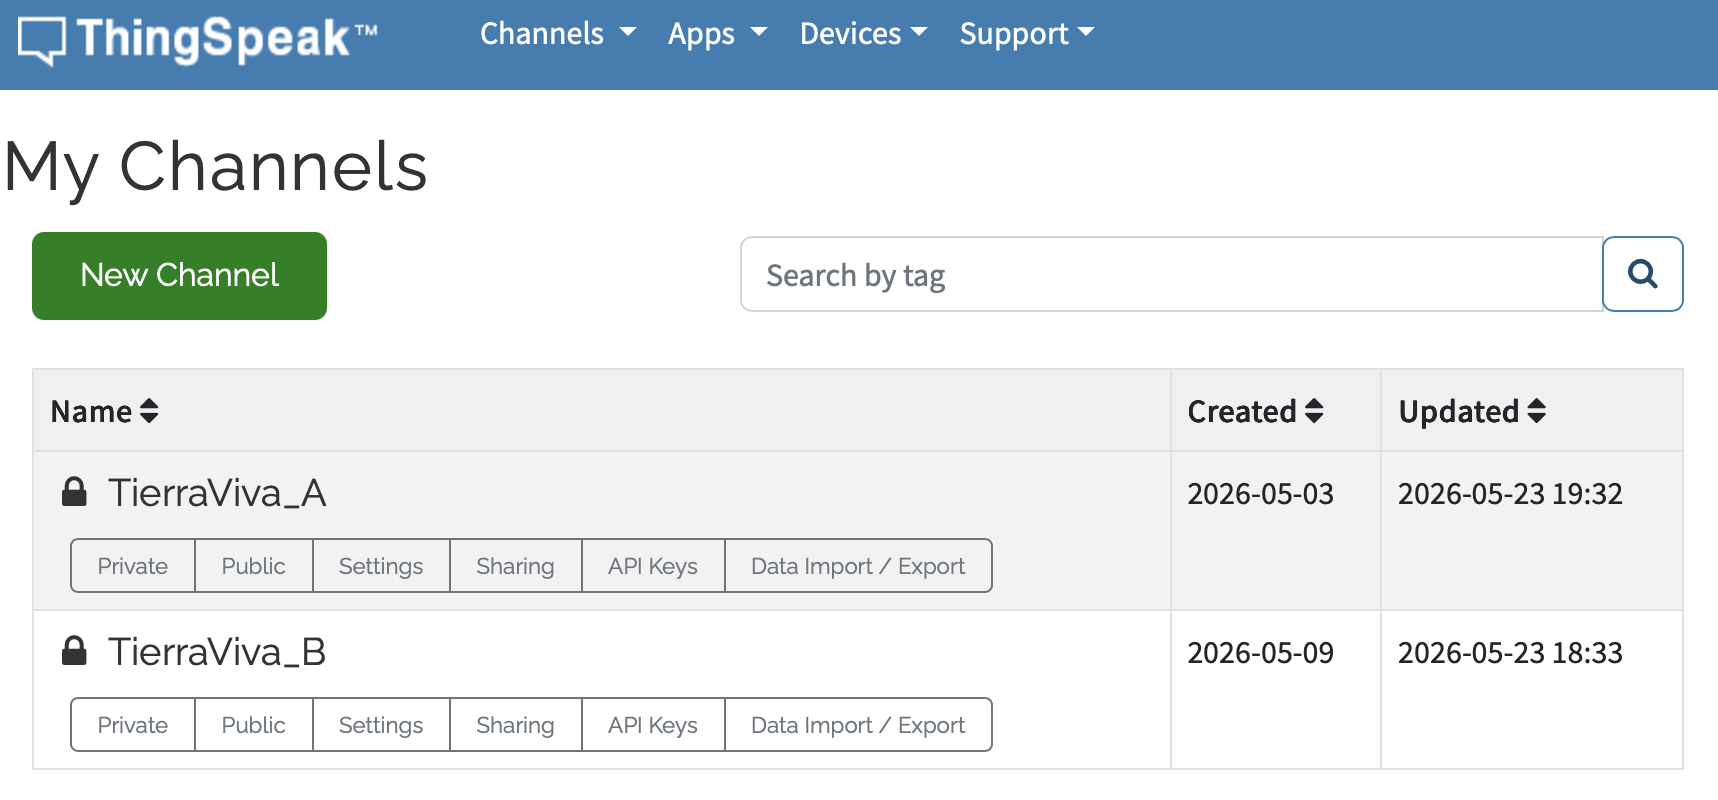
\includegraphics[width=0.90\textwidth]{figs/thingspeak_canales_tierraviva.png}
\caption{Canales ThingSpeak creados para las estaciones de TierraViva.}
\label{fig:thingspeak_canales_tierraviva}
\end{figure}

\subsection{Canales de estación}
\label{subsec:canales_estacion}

Los canales \texttt{TierraViva\_A} y \texttt{TierraViva\_B} almacenan la telemetría generada por las estaciones A y B, respectivamente. Cada actualización enviada por una estación incluye medidas del entorno y datos de estado, lo que permite a la Raspberry Pi supervisar tanto las variables ambientales como el comportamiento operativo del nodo.

\begin{table}[H]
\begin{center}
\small
\begin{tabular}{|p{0.18\textwidth}|p{0.28\textwidth}|p{0.44\textwidth}|}
\hline
\textbf{Campo} & \textbf{Dato} & \textbf{Descripción} \\
\hline
\texttt{field1} & Humedad del suelo normalizada (\%) & Valor calculado por el firmware a partir de la lectura bruta del sensor capacitivo. Se utiliza como entrada principal de la regla local de riego. \\
\hline
\texttt{field2} & Temperatura (\textdegree C) & Temperatura ambiente medida por el BME280. \\
\hline
\texttt{field3} & Humedad ambiente (\%) & Humedad relativa medida por el BME280. \\
\hline
\texttt{field4} & Luminosidad (lux) & Nivel de luz ambiente medido por el BH1750. \\
\hline
\texttt{field5} & Presión (hPa) & Presión atmosférica medida por el BME280. \\
\hline
\texttt{field6} & Estado del relé & Estado del relé asociado al bloque de actuación: \texttt{0} para apagado y \texttt{1} para activo. \\
\hline
\texttt{field7} & Modo seguro & Indicador de seguridad de la estación: \texttt{0} para funcionamiento normal y \texttt{1} para modo seguro activo. \\
\hline
\texttt{field8} & Código de estado & Código numérico que resume el estado operativo del ciclo o la incidencia detectada. \\
\hline
\end{tabular}
\caption{Asignación de campos en los canales ThingSpeak de estación}
\label{cuadro:canales_thingspeak_estacion}
\end{center}
\end{table}

La Tabla~\ref{cuadro:canales_thingspeak_estacion} define el contrato de datos utilizado por las estaciones. Mantener la misma estructura en ambos canales simplifica el firmware y la lógica de supervisión, ya que la Raspberry puede aplicar el mismo proceso de lectura para la estación A y para la estación B, cambiando únicamente el identificador del canal y la clave de lectura correspondiente.

Esta estructura permite que el canal no se limite a representar medidas ambientales. En particular, los campos \texttt{field6}, \texttt{field7} y \texttt{field8} aportan información operativa sobre el estado del relé, la activación del modo seguro y el código de estado publicado por la estación. Gracias a ello, la Raspberry puede detectar si una estación ha actuado, si está en reposo o si ha publicado una incidencia.

La separación por canales evita mezclar datos de estaciones distintas y facilita la escalabilidad. Si en el futuro se añadiese una nueva estación, bastaría con replicar la estructura de campos en un nuevo canal, asignar las claves correspondientes y ampliar la lógica de supervisión para incluir ese nuevo origen de datos.

\subsection{Descartes del control descendente desde la nube}
\label{subsec:decision_no_canales_comandos}

En fases anteriores del diseño se valoró utilizar ThingSpeak también como mecanismo de control descendente desde la Raspberry hacia las estaciones. En ese planteamiento, el sistema de supervisión publicaría instrucciones en la nube y cada estación tendría que consultarlas periódicamente. Aunque la solución era viable, añadía complejidad: obligaba a gestionar identificadores, evitar repeticiones, descartar información obsoleta y garantizar que una entrada antigua no provocase una actuación no deseada.

En la arquitectura final se descarta ese flujo descendente de control. Cada estación decide localmente si debe regar a partir de sus propias lecturas, umbrales, cooldown y condiciones de seguridad. Esta decisión simplifica el sistema y reduce la dependencia de la Raspberry Pi. Si la Raspberry se apaga o pierde conectividad, la estación no queda esperando una orden externa para mantener su comportamiento seguro.

ThingSpeak se mantiene, por tanto, como plataforma de telemetría y estado. Su papel no es transportar órdenes de riego, sino permitir que las estaciones publiquen su información y que la Raspberry pueda consultarla posteriormente. Esta separación hace que la nube sea importante para la supervisión, pero no imprescindible para que la estación ejecute sus reglas locales de seguridad.

En conjunto, ThingSpeak se utiliza en TierraViva como una capa intermedia sencilla pero suficiente para sostener el flujo de información del sistema. Los canales de estación permiten almacenar medidas y estados, la API HTTP facilita la integración con el A7670E-LASA y la lectura desde Raspberry Pi permite construir un histórico propio y un dashboard de supervisión.

\section{Raspberry Pi como sistema de supervisión}
\label{sec:raspberry_sistema_supervision}

La Raspberry Pi 5 actúa como sistema de supervisión de TierraViva. Su papel dentro de la arquitectura final no es sustituir a las estaciones de campo, conectarse físicamente a los sensores ni decidir la activación de la bomba, sino consultar la información disponible en la nube, mantener un histórico local, exponer una API y servir el dashboard web.

Esta separación es importante para mantener la coherencia del sistema distribuido. Las estaciones se encuentran en campo y se comunican mediante LTE/HTTP con ThingSpeak. La Raspberry, por tanto, no recibe datos por USB ni por puerto serie desde las estaciones, sino que consulta periódicamente los canales publicados en la plataforma cloud. A partir de esos datos, construye una visión actualizada del estado de cada estación.

El primer bloque funcional de la Raspberry es la lectura de datos desde ThingSpeak. Para cada estación, el sistema de supervisión consulta su canal correspondiente y obtiene las últimas medidas disponibles: humedad de suelo, temperatura, humedad relativa, luminosidad, presión atmosférica, estado del relé, código de estado y campo auxiliar. Esta lectura permite conocer tanto el estado ambiental de la zona monitorizada como el estado operativo de la estación.

Una vez recuperados los datos, la Raspberry debe validarlos antes de almacenarlos o mostrarlos. No todas las respuestas recibidas tienen por qué ser válidas: puede haber campos vacíos, valores fuera de rango, lecturas antiguas o errores de comunicación. Por ello, el sistema de supervisión debe comprobar que los datos recibidos son coherentes y que la marca temporal de la última lectura se encuentra dentro de un intervalo razonable. Si una estación no actualiza datos durante demasiado tiempo, el dashboard puede mostrarla como no disponible u obsoleta.

El segundo bloque funcional es el almacenamiento local en SQLite. Aunque ThingSpeak conserva las entradas publicadas en sus canales, TierraViva mantiene un histórico propio en la Raspberry Pi. Este histórico permite registrar las lecturas recibidas, los estados de relé, los eventos de riego publicados por las estaciones y las incidencias detectadas por el sistema de supervisión. De esta manera, la Raspberry no actúa únicamente como un visor de la nube, sino como un sistema con memoria propia del comportamiento del prototipo.

\begin{table}[H]
\begin{center}
\small
\begin{tabular}{|p{0.25\textwidth}|p{0.36\textwidth}|p{0.29\textwidth}|}
\hline
\textbf{Bloque} & \textbf{Función} & \textbf{Resultado esperado} \\
\hline
Lectura de ThingSpeak & Consulta periódica de los canales de las estaciones. & Últimas lecturas y estados disponibles. \\
\hline
Validación de datos & Comprobación de campos, rangos y antigüedad de las lecturas. & Detección de datos inválidos, ausentes u obsoletos. \\
\hline
SQLite & Almacenamiento local de lecturas, estados y eventos. & Histórico propio del sistema. \\
\hline
FastAPI & Exposición de datos mediante endpoints HTTP. & Respuestas estructuradas para el dashboard. \\
\hline
Dashboard web & Visualización del estado del sistema. & Interfaz de supervisión para el usuario. \\
\hline
\end{tabular}
\caption{Funciones principales de la Raspberry Pi dentro de TierraViva}
\label{cuadro:funciones_raspberry}
\end{center}
\end{table}

La API se desarrolla con FastAPI y actúa como capa intermedia entre la base de datos y el dashboard web. En lugar de que la interfaz consulte directamente SQLite o ThingSpeak, realiza peticiones a la API para obtener las últimas lecturas, el estado de las estaciones o el histórico necesario. Esta separación facilita la evolución del dashboard sin modificar la lógica de almacenamiento o consulta.

El dashboard web constituye la parte visible del sistema de supervisión. A través de él se pueden consultar las últimas medidas recibidas, comprobar el estado de cada estación, observar si existe comunicación reciente y revisar el estado del relé o los eventos de riego publicados por las estaciones. Su función no es ejecutar directamente acciones sobre el hardware, sino permitir la supervisión del sistema de forma clara. Esto resulta útil tanto durante las pruebas como en una posible utilización real del prototipo.

Además de almacenar lecturas, la Raspberry puede registrar incidencias de supervisión. Por ejemplo, puede detectar que una estación lleva demasiado tiempo sin publicar datos, que un campo llega vacío, que una lectura está fuera de rango o que el estado del relé no cambia durante un periodo esperado. Estos eventos no sustituyen a la lógica de seguridad local, pero ayudan a documentar el comportamiento del sistema y facilitan la validación experimental.

El ciclo completo de funcionamiento de la Raspberry puede resumirse en cuatro pasos. Primero, consulta los canales de ThingSpeak. Después, valida y almacena los datos recibidos en SQLite. A continuación, expone esa información mediante FastAPI. Finalmente, el dashboard web consulta la API y actualiza la visualización para el usuario.

Con esta organización, la Raspberry Pi queda como plataforma software de supervisión de TierraViva. Su valor no está en decidir cuándo se riega, sino en integrar datos, histórico, API y visualización. Esta decisión reduce la dependencia del sistema respecto a un único equipo central y deja la actuación física bajo control de la estación de campo, que es donde se encuentran los sensores, el relé y la bomba.

\section{Decisión local de riego y eventos}
\label{sec:decision_local_eventos}

La decisión de riego en TierraViva se ejecuta localmente en cada estación de campo. Esta elección elimina la necesidad de enviar comandos remotos desde la Raspberry Pi y desplaza la responsabilidad crítica al nodo que está físicamente conectado al sistema de riego. La estación dispone de las lecturas de sensores, controla el relé y puede actuar de forma inmediata sin depender de una comunicación continua con el exterior.

El criterio de decisión inicial se basa en una regla verificable de humedad del suelo. Si la lectura indica una condición de sequedad, no existe un periodo de espera activo y no se ha detectado ninguna incidencia, la estación puede activar el relé durante un tiempo limitado. Esta lógica no se plantea como inteligencia artificial, sino como automatización basada en reglas, adecuada para una primera versión del prototipo.

De forma conceptual, la decisión local puede resumirse así:

\begin{itemize}
    \item si la lectura de humedad del suelo cumple la condición de sequedad definida para el prototipo;
    \item si no existe un periodo de \textit{cooldown} activo;
    \item si la lectura de sensores es válida;
    \item si no se ha detectado un error crítico que afecte a los sensores, la alimentación o el estado seguro del relé;
    \item entonces la estación activa el relé durante un tiempo limitado y registra o publica el evento cuando la comunicación está disponible.
\end{itemize}

El uso de un \textit{cooldown} evita activaciones repetidas en poco tiempo. Esta medida es necesaria porque las lecturas de humedad pueden oscilar alrededor del umbral o variar lentamente tras una actuación. Sin un periodo mínimo entre riegos, la estación podría activar la bomba varias veces de forma consecutiva. Por tanto, el firmware debe registrar el instante de la última actuación y bloquear nuevos riegos hasta que se supere el tiempo mínimo configurado.

La duración del riego se controla también desde el firmware. La estación no debe mantener el relé activo de forma indefinida ni depender de una orden externa de parada. El comportamiento seguro consiste en activar el relé, esperar como máximo el tiempo permitido y desactivarlo siempre al finalizar la actuación. Si durante ese proceso se detecta una condición anómala, el relé debe apagarse de forma inmediata.

Tras cada ciclo, la estación publica en ThingSpeak no solo las medidas ambientales, sino también información de estado. Esto permite que la Raspberry Pi supervise lo ocurrido sin participar en la decisión. En particular, el campo de estado o evento permite distinguir entre funcionamiento normal, riego ejecutado, cooldown activo, lectura inválida, error de sensor o activación bloqueada por seguridad.

\begin{table}[H]
\begin{center}
\small
\begin{tabular}{|p{0.18\textwidth}|p{0.34\textwidth}|p{0.38\textwidth}|}
\hline
\textbf{Código} & \textbf{Significado} & \textbf{Interpretación} \\
\hline
\texttt{0} & Funcionamiento normal & La estación mide y publica sin incidencias. \\
\hline
\texttt{1} & Sensor no disponible & Algún sensor no responde o no se ha podido obtener la lectura esperada. \\
\hline
\texttt{2} & Incidencia de comunicación & La estación ha detectado un fallo de publicación o inicialización de red y lo registra para supervisión. \\
\hline
\texttt{3} & Riego ejecutado & La estación ha activado el relé durante el tiempo permitido. \\
\hline
\texttt{4} & Riego no necesario & La humedad no cumple la condición de sequedad. \\
\hline
\texttt{5} & Lectura no válida para decisión & La lectura existe, pero se descarta por ser incoherente, fuera de rango o no fiable para activar el riego. \\
\hline
\texttt{6} & Cooldown activo & La estación evita un nuevo riego por periodo mínimo entre actuaciones. \\
\hline
\texttt{7} & Apagado de seguridad & El firmware fuerza el relé a apagado por condición no verificable. \\
\hline
\end{tabular}
\caption{Códigos de estado o evento publicados por las estaciones}
\label{cuadro:codigos_estado_evento}
\end{center}
\end{table}

La Tabla~\ref{cuadro:codigos_estado_evento} recoge una codificación inicial para interpretar el estado publicado por las estaciones. Estos códigos no tienen por qué representar errores graves; en algunos casos, como el código de cooldown o el de riego no necesario, simplemente permiten explicar por qué la estación no ha activado la bomba en un ciclo concreto.

Esta forma de funcionamiento ofrece trazabilidad sin necesidad de comandos remotos. La Raspberry Pi puede reconstruir qué ha ocurrido observando las lecturas, el estado del relé y el código de evento publicado por cada estación. Así se mantiene una separación clara entre decisión local y supervisión: la estación decide y actúa, mientras que la Raspberry registra y muestra.

\section{Modo seguro}
\label{sec:modo_seguro}

El modo seguro de TierraViva define el comportamiento que debe adoptar la estación cuando no puede garantizar que una actuación sobre el riego sea correcta. Este punto es especialmente importante porque el prototipo no se limita a monitorizar variables ambientales, sino que incorpora actuación física mediante relé y bomba de agua. Por tanto, un fallo en sensores, alimentación, comunicación o lógica interna no debe traducirse en una activación indefinida del riego.

El criterio general adoptado es conservador: ante una situación no verificable, la bomba debe permanecer apagada. Esta decisión puede provocar que el sistema no riegue en un caso dudoso, pero evita el escenario de mayor riesgo para el prototipo, que sería mantener el riego activo sin control. En este proyecto se considera preferible perder una actuación puntual antes que activar la bomba de forma repetida o indefinida.

El modo seguro se aplica tanto en el arranque de la estación como durante el funcionamiento normal. Al iniciar el firmware, el pin de control del relé debe configurarse en estado desactivado antes de procesar sensores o comunicaciones. De esta forma, un reinicio de la placa no provoca una activación accidental de la bomba. El estado inicial del sistema es, por tanto, relé desactivado y bomba apagada.

\begin{table}[H]
\begin{center}
\small
\begin{tabular}{|p{0.30\textwidth}|p{0.33\textwidth}|p{0.27\textwidth}|}
\hline
\textbf{Situación detectada} & \textbf{Riesgo asociado} & \textbf{Respuesta segura} \\
\hline
Arranque o reinicio de la estación & Activación accidental del relé durante la inicialización. & Relé desactivado y bomba apagada. \\
\hline
Lectura de sensor inválida & Decisión de riego basada en un dato no fiable. & No iniciar riego y publicar estado de error si la comunicación está disponible. \\
\hline
Lectura fuera de rango & Interpretación incorrecta del estado del suelo. & Ignorar lectura y mantener bomba apagada. \\
\hline
Cooldown activo & Activaciones repetidas por oscilación de la medida. & No iniciar nuevo riego. \\
\hline
Tiempo máximo alcanzado & Riego indefinido por fallo de control o bloqueo del programa. & Desactivar relé al superar el límite. \\
\hline
Pérdida de comunicación & Falta de supervisión remota o publicación fallida. & Mantener comportamiento local seguro y registrar incidencia cuando sea posible. \\
\hline
Error interno & Estado no fiable de sensores, comunicación o lógica local. & Forzar relé a apagado y publicar código de seguridad si es posible. \\
\hline
\end{tabular}
\caption{Situaciones contempladas por el modo seguro de la estación}
\label{cuadro:modo_seguro}
\end{center}
\end{table}

La Tabla~\ref{cuadro:modo_seguro} resume las situaciones principales contempladas. Todas las respuestas siguen el mismo criterio: si el sistema no puede verificar que la actuación sea correcta, no debe activar la bomba.

La pérdida de comunicación se interpreta de forma distinta a como ocurriría en una arquitectura centralizada. En TierraViva, la estación no necesita recibir una orden externa para decidir el riego, por lo que una caída temporal de la Raspberry o de la supervisión remota no bloquea necesariamente la lógica local. Sin embargo, si el módulo LTE no puede publicar datos durante un periodo prolongado, el firmware debe registrar la incidencia cuando la comunicación vuelva a estar disponible y mantener siempre el relé bajo control local. La pérdida de supervisión remota no debe dejar la bomba activa ni provocar una actuación no controlada; en caso de duda sobre el estado interno de la estación, se mantiene la bomba apagada.

Las lecturas inválidas constituyen otro caso crítico. Si el sensor de humedad devuelve un valor ausente, imposible o fuera del rango esperado, la estación no debe utilizar ese dato para activar la bomba. En su lugar, debe publicar un código de error o conservar el estado seguro hasta que las lecturas vuelvan a ser coherentes. Esta medida evita que una desconexión del sensor o una lectura corrupta se interprete como necesidad real de riego.

El tiempo máximo de actuación es una barrera de seguridad esencial. Aunque la regla local determine que el suelo está seco, la bomba solo puede permanecer activa durante el intervalo permitido. Finalizado ese tiempo, el relé debe desactivarse siempre. Esta desactivación no debe depender de la Raspberry Pi ni de ThingSpeak, sino del propio firmware de la estación.

El cooldown complementa al tiempo máximo. Tras una actuación, la estación debe esperar un periodo mínimo antes de volver a regar. Esto reduce el riesgo de activaciones repetidas provocadas por ruido, histéresis insuficiente o lenta estabilización de la humedad del suelo después del riego.

El modo seguro actúa, por tanto, como una capa local de protección. La Raspberry Pi puede supervisar, registrar y mostrar el estado del sistema, pero la estación conserva la responsabilidad última sobre la decisión y la ejecución segura de la actuación. Esta decisión es coherente con la arquitectura final de TierraViva: autonomía en campo, comunicación para supervisión y seguridad prioritaria frente a cualquier estado dudoso.


\chapter{Implementación hardware y firmware de estaciones}
\label{cap:implementacion_hardware_firmware}

Una vez definida la arquitectura final del sistema, este capítulo describe la implementación hardware y firmware de las estaciones de campo de TierraViva. El propósito no es repetir las decisiones de diseño ya justificadas en capítulos anteriores, sino documentar cómo se preparó, conectó y validó cada bloque de la estación: controlador, sensores, comunicación LTE, publicación de telemetría, actuación sobre el riego y alimentación.

En la arquitectura final, la estación no es un simple nodo que obedece instrucciones externas. Cada estación debe medir, evaluar reglas locales, accionar el riego cuando corresponda y publicar su estado. Por ello, la implementación hardware y el firmware tienen un papel central dentro del prototipo.

\begin{wrapfigure}{r}{0.22\textwidth}
    \vspace{-12pt}
    \centering
    
\includegraphics[width=0.20\textwidth]{figs/arduino_logo.png}
    \caption{Logo Arduino}
    \label{fig:logo_arduino}
    \vspace{-8pt}
\end{wrapfigure}

La implementación se ha desarrollado de forma incremental. En primer lugar, se preparó el entorno de trabajo con Arduino UNO y se comprobó la programación básica de la placa. A continuación, se validaron los sensores de forma individual y conjunta, se integró el módulo de comunicaciones LTE A7670E-LASA, se implementó el envío de telemetría hacia ThingSpeak y se preparó la lógica de actuación mediante relé y bomba de agua. Esta secuencia permitió reducir riesgos, ya que cada bloque fue probado antes de incorporarse al firmware completo de la estación.

\section{Preparación de Arduino UNO}
\label{sec:preparacion_arduino_uno}

La primera fase de implementación consistió en preparar la placa Arduino UNO que actúa como controlador local de la estación de campo. Antes de conectar sensores, módulo LTE o relé, era necesario comprobar que el entorno de programación reconocía correctamente la placa y que era posible cargar un programa básico sin errores. Esta comprobación inicial evita arrastrar problemas de comunicación USB o configuración del entorno a fases posteriores del montaje.

El entorno de desarrollo utilizado fue Arduino IDE 2.3.8 sobre Windows 11. La placa empleada no fue una Arduino UNO oficial, sino una placa compatible basada en el microcontrolador ATmega328P. Este tipo de placas es habitual en prototipos de bajo coste, pero puede requerir una preparación adicional cuando el conversor USB-serie no es reconocido automáticamente por el sistema operativo.

Durante la primera conexión por USB, la placa recibía alimentación y encendía sus indicadores luminosos, pero no aparecía ningún puerto disponible en el menú \textit{Tools} $\rightarrow$ \textit{Port} del Arduino IDE. Esto indicaba que el ordenador detectaba alimentación eléctrica, pero no disponía todavía de una comunicación serie utilizable para programar la placa.

La comprobación en el Administrador de dispositivos de Windows mostró el dispositivo como \texttt{USB2.0-Serial} dentro del apartado de otros dispositivos. Esta situación permitió identificar el problema: el sistema no tenía instalado el controlador correspondiente al conversor USB-serie de la placa. La inspección física del Arduino confirmó que el chip situado junto al conector USB era un \texttt{CH340G}, mientras que el microcontrolador principal era un \texttt{ATmega328P}.

\begin{table}[H]
\begin{center}
\small
\begin{tabular}{|p{0.30\textwidth}|p{0.30\textwidth}|p{0.30\textwidth}|}
\hline
\textbf{Elemento comprobado} & \textbf{Resultado observado} & \textbf{Acción realizada} \\
\hline
Sistema operativo & Windows 11 & Preparación del entorno en PC. \\
\hline
Entorno de desarrollo & Arduino IDE 2.3.8 & Instalación y configuración inicial. \\
\hline
Placa conectada & Arduino UNO compatible & Selección de placa Arduino Uno. \\
\hline
Detección inicial & \texttt{USB2.0-Serial} sin puerto COM disponible & Diagnóstico de falta de driver. \\
\hline
Conversor USB-serie & \texttt{CH340G} & Instalación del driver CH340/CH341. \\
\hline
Microcontrolador principal & \texttt{ATmega328P} & Validación de compatibilidad con Arduino UNO. \\
\hline
Puerto tras instalar driver & \texttt{COM3} & Selección del puerto en Arduino IDE. \\
\hline
Prueba básica & \textit{Blink} cargado correctamente & Verificación de programación de la placa. \\
\hline
\end{tabular}
\caption{Preparación inicial del Arduino UNO compatible}
\label{cuadro:preparacion_arduino_uno}
\end{center}
\end{table}

Una vez identificado el chip \texttt{CH340G}, se instaló el driver CH340/CH341 correspondiente. Tras reconectar la placa, Windows pasó a reconocerla como un dispositivo serie asociado al puerto \texttt{COM3}. A partir de ese momento, el Arduino IDE permitió seleccionar la placa como \textit{Arduino Uno} y utilizar el puerto serie correcto para la carga de programas.

La primera prueba realizada fue el ejemplo \textit{Blink}, incluido en el propio Arduino IDE. Esta prueba consiste en cargar un programa sencillo que conmuta periódicamente el LED integrado de la placa. Aunque funcionalmente es una prueba mínima, resulta útil como validación de la cadena completa de programación: detección USB, selección de placa, selección de puerto, compilación, carga del programa y ejecución en el microcontrolador.

El resultado fue correcto: el programa se cargó en la placa a través de \texttt{COM3} y el LED integrado respondió según lo esperado. Además, el registro de carga mostró la comunicación con el microcontrolador \texttt{ATmega328P}, confirmando que la placa era programable desde el entorno configurado. Esta validación permitió continuar con las pruebas de sensores sin que la conexión USB o el driver fueran una fuente de error adicional.

Desde el punto de vista de documentación del proyecto, esta incidencia es relevante porque refleja una condición real del montaje. El uso de placas compatibles reduce el coste del prototipo, pero puede introducir pequeños problemas de preparación, como la necesidad de instalar drivers adicionales. Registrar este paso mejora la reproducibilidad del trabajo, ya que otra persona que replique el sistema podría encontrarse con el mismo síntoma: placa encendida, pero sin puerto COM disponible.

Las evidencias de esta fase se integrarán en el registro de resultados del Anexo~\ref{anexo:plan_pruebas}, junto con las capturas del Administrador de dispositivos, la configuración del Arduino IDE y las fotografías de la placa.

Con la placa correctamente reconocida y la prueba \textit{Blink} superada, el Arduino UNO quedó preparado para la siguiente fase: la conexión y validación de los sensores de la estación de campo. Esta comprobación permitió utilizar la placa como base del firmware autónomo de TierraViva, encargado posteriormente de leer sensores, comunicarse con el módulo LTE, controlar el relé y aplicar la lógica local de riego.

\section{Integración de sensores}
\label{sec:integracion_sensores}

Una vez preparada la placa Arduino UNO, la siguiente fase consistió en integrar y validar los sensores de la estación de campo. Esta etapa era necesaria antes de incorporar la comunicación LTE o la actuación sobre el riego, ya que el sistema completo depende de que las medidas de entrada sean coherentes. En TierraViva se utilizan tres bloques de sensórica: humedad de suelo, variables ambientales y luminosidad.

La integración se realizó de forma incremental. Primero se comprobó el bus I2C, después se validó el sensor de humedad de suelo mediante lectura analógica y, por último, se ejecutó una prueba conjunta con todos los sensores conectados. Este procedimiento permitió aislar fallos de cableado o configuración antes de pasar a un firmware más completo.

El BME280 y el BH1750 se conectan mediante el bus I2C del Arduino UNO. I2C, abreviatura de \textit{Inter-Integrated Circuit}, es un bus de comunicación serie utilizado habitualmente para conectar sensores y circuitos integrados con un microcontrolador empleando únicamente dos líneas principales: \texttt{SDA}, para el intercambio de datos, y \texttt{SCL}, para la señal de reloj. En este tipo de bus, varios dispositivos pueden compartir las mismas líneas siempre que cada uno tenga una dirección diferente.

En Arduino UNO, las líneas I2C corresponden a los pines \texttt{A4/SDA} y \texttt{A5/SCL}, según la documentación oficial de la placa \cite{arduino_uno_r3_pinout,arduino_uno_r3_datasheet}. Por este motivo, el BME280 y el BH1750 pueden conectarse simultáneamente a los mismos pines. En el montaje realizado, el BH1750 fue detectado en la dirección \texttt{0x23} y el BME280 en la dirección \texttt{0x76}, por lo que ambos sensores pudieron trabajar en el mismo bus sin conflicto de direcciones.

El sensor capacitivo de humedad de suelo se conectó de forma independiente al bus I2C, ya que proporciona una salida analógica. Para esta prueba se utilizó la entrada \texttt{A0} del Arduino UNO. Esta lectura no representa directamente un porcentaje de humedad, sino un valor bruto entre 0 y 1023, correspondiente al convertidor analógico-digital del microcontrolador. Por ello, antes de utilizarlo como porcentaje de humedad es necesario realizar una calibración o, al menos, identificar el sentido de variación de la medida.

La Tabla~\ref{cuadro:cableado_sensores} resume las conexiones utilizadas durante la integración de sensores.

\begin{table}[H]
\begin{center}
\small
\begin{tabular}{|p{0.24\textwidth}|p{0.24\textwidth}|p{0.32\textwidth}|}
\hline
\textbf{Sensor} & \textbf{Conexión Arduino UNO} & \textbf{Función} \\
\hline
BME280 & \texttt{VCC} a 5 V, \texttt{GND} a GND, \texttt{SDA} a \texttt{A4}, \texttt{SCL} a \texttt{A5} & Medición de temperatura, humedad relativa y presión atmosférica. \\
\hline
BH1750 / GY-302 & \texttt{VCC} a 5 V, \texttt{GND} a GND, \texttt{SDA} a \texttt{A4}, \texttt{SCL} a \texttt{A5} & Medición de luminosidad ambiente en lux. \\
\hline
Sensor capacitivo de humedad de suelo & \texttt{VCC} a 5 V, \texttt{GND} a GND, \texttt{AO} a \texttt{A0} & Lectura analógica del estado del sustrato. \\
\hline
\end{tabular}
\caption{Conexiones de los sensores integrados en la estación de campo}
\label{cuadro:cableado_sensores}
\end{center}
\end{table}

Durante las pruebas se tuvo en cuenta que todos los módulos deben compartir una referencia común de masa. Este punto es importante porque una referencia de GND incorrecta puede producir lecturas inestables o impedir la comunicación con los sensores digitales. En el caso del bus I2C, también se comprobó que no era necesario utilizar pines alternativos para \texttt{SDA} y \texttt{SCL}, ya que en Arduino UNO el bus hardware está asignado a \texttt{A4} y \texttt{A5}.

La primera comprobación realizada sobre los sensores digitales fue un escaneo del bus I2C. Esta prueba no mide todavía variables físicas, pero permite verificar que los dispositivos están correctamente alimentados, cableados y accesibles desde Arduino. El resultado obtenido fue la detección de dos dispositivos: \texttt{0x23}, correspondiente al BH1750, y \texttt{0x76}, correspondiente al BME280.

\begin{table}[H]
\begin{center}
\small
\begin{tabular}{|p{0.28\textwidth}|p{0.28\textwidth}|p{0.34\textwidth}|}
\hline
\textbf{Prueba} & \textbf{Resultado} & \textbf{Interpretación} \\
\hline
Escaneo I2C con BME280 & Dispositivo detectado en \texttt{0x76} & El sensor ambiental responde correctamente en el bus I2C. \\
\hline
Escaneo I2C con BH1750 y BME280 & Dispositivos detectados en \texttt{0x23} y \texttt{0x76} & Ambos sensores pueden compartir el bus I2C sin conflicto de direcciones. \\
\hline
Lectura analógica del sensor de suelo & Valores variables en \texttt{A0} & El sensor capacitivo responde ante cambios de capacitancia/humedad. \\
\hline
Prueba conjunta & Lectura de suelo, luz, temperatura, humedad y presión & Los tres sensores pueden integrarse en un único firmware de adquisición. \\
\hline
\end{tabular}
\caption{Pruebas iniciales de validación de sensores}
\label{cuadro:pruebas_iniciales_sensores}
\end{center}
\end{table}

El sensor de humedad de suelo se probó inicialmente mediante un sketch específico que imprimía por el monitor serie el valor bruto leído en \texttt{A0}. En reposo, el sensor mostró valores estables alrededor de \texttt{569--570}. Al tocar la zona sensible del sensor, los valores descendieron aproximadamente al rango \texttt{248--356}. Esta prueba confirmó que el sensor respondía ante cambios físicos y permitió identificar el sentido de variación: en el montaje probado, un aumento de capacitancia asociado a mayor humedad o contacto produce una disminución del valor analógico leído.

Esta prueba no debe interpretarse como una calibración definitiva de humedad de suelo. Para convertir el valor bruto en un porcentaje fiable sería necesario medir el sensor en condiciones controladas, por ejemplo en aire, en suelo seco y en suelo húmedo, manteniendo la electrónica protegida del agua. Sin embargo, para esta fase de integración, el resultado fue suficiente para comprobar que el sensor estaba vivo, conectado al pin correcto y entregaba una señal analógica utilizable.

El BH1750 se integró como sensor digital de luminosidad. Su lectura se realiza en lux, por lo que resulta más directa que la del sensor de suelo. Durante las pruebas conjuntas, este sensor se inicializó en modo de alta resolución continua mediante la librería correspondiente. Además, al estar conectado al mismo bus que el BME280, su detección en \texttt{0x23} permitió confirmar que no existía conflicto con la dirección \texttt{0x76} del sensor ambiental.

El BME280 se utilizó para obtener temperatura, humedad relativa y presión atmosférica. En el firmware de prueba se inicializó mediante la dirección \texttt{0x76}. Esta comprobación era relevante porque algunos módulos comerciales se anuncian como BME/BMP280 y pueden generar dudas durante el montaje. En el caso de TierraViva, la integración se preparó utilizando la librería del BME280, ya que el sistema necesita también la humedad relativa ambiental, no solo temperatura y presión.

Tras validar los sensores por separado, se cargó un sketch integrado para leer todos los valores en una misma ejecución. Este programa inicializaba el bus I2C, configuraba el BH1750, configuraba el BME280 y leía el sensor de suelo en \texttt{A0}. La salida por monitor serie se estructuró en una línea con los campos principales: \texttt{soil\_raw}, \texttt{lux}, \texttt{temp\_c}, \texttt{hum\_pct} y \texttt{pres\_hpa}. Esta forma de imprimir los datos facilita la depuración y deja preparada la estructura para fases posteriores, donde las lecturas deben enviarse como telemetría.

\begin{table}[H]
\begin{center}
\small
\begin{tabular}{|p{0.24\textwidth}|p{0.28\textwidth}|p{0.38\textwidth}|}
\hline
\textbf{Variable} & \textbf{Origen} & \textbf{Uso dentro de la estación} \\
\hline
\texttt{soil\_raw} & Sensor capacitivo en \texttt{A0} & Variable principal para interpretar el estado del sustrato. \\
\hline
\texttt{lux} & BH1750 & Información sobre la exposición luminosa del entorno. \\
\hline
\texttt{temp\_c} & BME280 & Temperatura ambiente en grados Celsius. \\
\hline
\texttt{hum\_pct} & BME280 & Humedad relativa ambiental en porcentaje. \\
\hline
\texttt{pres\_hpa} & BME280 & Presión atmosférica en hectopascales. \\
\hline
\end{tabular}
\caption{Variables obtenidas en la prueba conjunta de sensores}
\label{cuadro:variables_prueba_conjunta_sensores}
\end{center}
\end{table}

La integración conjunta permitió comprobar que el sensor analógico no interfería con el bus I2C y que los sensores digitales podían trabajar simultáneamente. Esta prueba es importante porque el firmware final de la estación no lee los sensores de forma aislada, sino que debe construir una muestra completa de telemetría en cada ciclo de adquisición.

Desde el punto de vista de interpretación de datos, la humedad de suelo requiere especial atención. A diferencia de la temperatura o la luminosidad, que se obtienen en unidades físicas directamente interpretables, el sensor capacitivo entrega un valor dependiente del propio sensor, del suelo, de la alimentación y de las condiciones de montaje. Por ello, en las primeras pruebas se mantuvo como \texttt{soil\_raw}. Más adelante, este valor puede transformarse en porcentaje mediante una calibración con valores de referencia seco y húmedo.

También se decidió mantener las variables ambientales como información de contexto. La temperatura, la humedad relativa, la presión y la luminosidad no determinan por sí solas la activación del riego en esta fase, pero permiten interpretar mejor el estado de la estación. Por ejemplo, una humedad de suelo baja puede tener consecuencias distintas en un momento de baja luminosidad que en una situación de alta exposición solar y temperatura elevada.

Con esta prueba quedó validado el bloque de sensórica de la estación. Se confirmó la comunicación I2C con el BME280 y el BH1750, la lectura analógica del sensor de humedad de suelo y la posibilidad de obtener todas las variables en un único ciclo de adquisición. Con ello, la estación quedó preparada para el siguiente paso de implementación: estructurar el firmware de adquisición y adaptar las lecturas al formato de telemetría utilizado por TierraViva.

\section{Firmware de adquisición}
\label{sec:firmware_adquisicion}

Una vez comprobado el funcionamiento de los sensores, el siguiente paso consistió en organizar el firmware de adquisición de la estación. Este firmware no se limita a leer variables y enviarlas a la nube, sino que también incorpora la lógica local mínima necesaria para decidir si debe activarse el riego.

El firmware se organiza en varios bloques funcionales. En primer lugar, se inicializan los sensores y el módem LTE. Después, en cada ciclo de ejecución, se leen las variables ambientales y de suelo. A partir de esas lecturas, se actualiza el estado interno de seguridad de la estación y se decide si procede activar el riego. Por último, la estación publica una actualización en ThingSpeak con las medidas y el estado operativo.

\begin{table}[H]
\begin{center}
\small
\begin{tabular}{|p{0.28\textwidth}|p{0.57\textwidth}|}
\hline
\textbf{Bloque del firmware} & \textbf{Función principal} \\
\hline
Inicialización & Configurar puerto serie, bus I2C, sensores, pin del relé y módulo LTE. \\
\hline
Adquisición & Leer humedad de suelo, temperatura, humedad relativa, luminosidad y presión. \\
\hline
Interpretación & Convertir la lectura del sensor de suelo a una escala porcentual y comprobar la validez de las medidas. \\
\hline
Decisión local & Evaluar umbrales, ciclos de confirmación, cooldown y estado seguro. \\
\hline
Actuación & Activar el relé durante un tiempo limitado cuando procede el riego. \\
\hline
Telemetría & Enviar a ThingSpeak las variables medidas y el estado operativo de la estación. \\
\hline
\end{tabular}
\caption{Bloques principales del firmware de adquisición y decisión local}
\label{cuadro:bloques_firmware_adquisicion}
\end{center}
\end{table}

La inicialización se realiza en la función \texttt{setup()}. En esta fase se configura el puerto serie de depuración, se inicializa el bus I2C, se comprueba la disponibilidad de los sensores y se prepara el pin de control del relé. Un punto importante es que el relé debe quedar en estado desactivado desde el arranque. De esta forma, \textbf{un reinicio del Arduino no puede provocar una activación accidental de la bomba}.

El bloque de adquisición lee las mismas variables validadas en el apartado anterior. La humedad de suelo se obtiene a partir del sensor capacitivo conectado a la entrada analógica. El BME280 proporciona temperatura, humedad relativa y presión atmosférica. El BH1750 proporciona la luminosidad ambiente en lux. Estas medidas se almacenan en variables internas del firmware para poder ser utilizadas tanto en la decisión local como en la publicación de telemetría.

En el caso de la humedad de suelo, el firmware no trabaja únicamente con el valor bruto del conversor analógico-digital. A partir de los valores de referencia obtenidos durante las pruebas, la lectura se transforma a una escala porcentual mediante una función de conversión. Esta transformación facilita la interpretación posterior: un valor bajo de porcentaje indica una situación de suelo seco, mientras que un valor más alto representa mayor humedad del sustrato.

El firmware también mantiene un modo seguro local. Este modo no es una orden recibida desde la Raspberry Pi, sino un estado interno de la estación. Se activa cuando las lecturas no son fiables o cuando el sistema todavía no ha acumulado suficientes ciclos válidos tras el arranque. En modo seguro, la estación utiliza un criterio más conservador para permitir el riego.

En el código, esta lógica se refleja mediante variables como \texttt{safeMode}, \texttt{sensorOk}, \texttt{validCycleCount} y \texttt{dryCycleCount}. Además, el firmware diferencia entre el evento principal del sistema, almacenado en \texttt{systemEventCode}, y el código auxiliar de diagnóstico, almacenado en \texttt{debugCode}. Esta separación permite publicar en ThingSpeak no solo si la estación está regando o no, sino también el motivo de la decisión.

La lógica de lectura de sensores se muestra en el Código~\ref{cod:lectura_sensores_estacion}. En esta versión, el firmware calcula la humedad del suelo a partir de la lectura analógica, lee las variables ambientales y marca la lectura como no válida si alguno de los sensores devuelve un valor incoherente.

\begin{code}[H]
\begin{lstlisting}[language=C++]
void readSensors() {
  sensorOk = true;

  soilRawValue = readSoilRaw();
  soilPercent = soilRawToPercent(soilRawValue);

  float t = bme.readTemperature();
  float h = bme.readHumidity();
  float p = bme.readPressure();
  float l = lightMeter.readLightLevel();

  if (isnan(t) || isnan(h) || isnan(p) || l < 0) {
    sensorOk = false;
  } else {
    temperatureC = t;
    humidityPct = h;
    pressureHpa = (int)(p / 100.0F + 0.5);
    luxValue = (int)(l + 0.5);
  }

  if (!sensorOk) {
    temperatureC = 0.0;
    humidityPct = 0.0;
    pressureHpa = 0;
    luxValue = 0;
  }
}
\end{lstlisting}
\caption[Lectura agrupada de sensores en la estación]{Lectura agrupada de sensores en la estación}
\label{cod:lectura_sensores_estacion}
\end{code}

La decisión local se apoya en tres mecanismos: umbral de humedad, confirmación por ciclos consecutivos y tiempo mínimo entre riegos. No se activa el riego por una única lectura aislada, ya que una medida puntual puede verse afectada por ruido, contacto irregular del sensor o pequeñas variaciones del montaje. Por ello, el firmware acumula ciclos consecutivos en los que el suelo aparece seco antes de considerar que realmente procede regar.

Además, se incorpora un periodo de \textit{cooldown}. Después de un riego, la estación bloquea nuevas activaciones durante un tiempo mínimo. Esta medida evita ciclos repetidos de riego en poco tiempo y reduce el riesgo de sobreactuación.

\begin{code}[H]
\begin{lstlisting}[language=C++]
bool cooldownActive() {
  if (lastIrrigationEndMs == 0) return false;
  return (millis() - lastIrrigationEndMs) < COOLDOWN_MS;
}
\end{lstlisting}
\caption[Comprobación del periodo de espera entre riegos]{Comprobación del periodo de espera entre riegos}
\label{cod:cooldown_riego}
\end{code}

El modo seguro se actualiza en cada ciclo a partir del estado de los sensores y del número de ciclos válidos acumulados. Si los sensores no son fiables, el sistema permanece en modo seguro. Si se acumulan varios ciclos correctos, la estación puede volver al funcionamiento normal.

\begin{code}[H]
\begin{lstlisting}[language=C++]
void updateSafetyState() {
  if (!sensorOk) {
    safeMode = true;
    validCycleCount = 0;
    dryCycleCount = 0;
    return;
  }

  validCycleCount++;

  if (safeMode && validCycleCount >= SAFE_EXIT_VALID_CYCLES) {
    safeMode = false;
    dryCycleCount = 0;
  }

  int threshold = safeMode ? SAFE_SOIL_THRESHOLD
                           : NORMAL_SOIL_THRESHOLD;

  if (soilPercent <= threshold) {
    if (dryCycleCount < 255) dryCycleCount++;
  } else {
    dryCycleCount = 0;
  }
}
\end{lstlisting}
\caption[Actualización del modo seguro y ciclos de suelo seco]{Actualización del modo seguro y ciclos de suelo seco}
\label{cod:update_safety_state}
\end{code}

La función de decisión local se muestra en el Código~\ref{cod:decision_local_riego}. Si existe un error de sensores o un periodo de cooldown activo, la estación no permite el riego y actualiza los códigos de estado correspondientes. Si no existe bloqueo, compara la humedad del suelo con el umbral normal o seguro según el estado interno de la estación.

\begin{code}[H]
\begin{lstlisting}[language=C++]
bool shouldIrrigate() {
  if (!sensorOk) {
    systemEventCode = 400;
    debugCode = 400;
    return false;
  }

  if (cooldownActive()) {
    systemEventCode = 429;
    debugCode = 429;
    return false;
  }

  if (safeMode) {
    return (soilPercent <= SAFE_SOIL_THRESHOLD) &&
           (dryCycleCount >= SAFE_CONFIRM_DRY_CYCLES);
  }

  return (soilPercent <= NORMAL_SOIL_THRESHOLD) &&
         (dryCycleCount >= NORMAL_CONFIRM_DRY_CYCLES);
}
\end{lstlisting}
\caption[Decisión local de riego en la estación]{Decisión local de riego en la estación}
\label{cod:decision_local_riego}
\end{code}

Cuando la estación decide regar, la actuación se realiza de forma local mediante el relé. El Código~\ref{cod:activacion_temporizada_rele} muestra la activación temporizada utilizada en el firmware actual. Durante el riego, el evento principal se marca como \texttt{210}; al finalizar, el relé se apaga y el evento pasa a \texttt{211}.

\begin{code}[H]
\begin{lstlisting}[language=C++]
void irrigateForSeconds(unsigned long seconds) {
  relayActive = true;
  digitalWrite(RELAY_PIN, RELAY_ON);

  systemEventCode = 210; // riego encendido
  debugCode = 200;

  delay(seconds * 1000UL);

  digitalWrite(RELAY_PIN, RELAY_OFF);
  relayActive = false;
  lastIrrigationEndMs = millis();

  systemEventCode = 211; // riego finalizado
  debugCode = 200;
}
\end{lstlisting}
\caption[Activación temporizada del relé de riego]{Activación temporizada del relé de riego}
\label{cod:activacion_temporizada_rele}
\end{code}

Tras la lectura de sensores, la actualización del modo seguro y la posible actuación sobre el relé, el firmware prepara el estado de la estación para su publicación. Esta publicación no se desarrolla en detalle en esta sección para evitar duplicidades, ya que la correspondencia completa entre variables y campos de ThingSpeak se documenta en la Sección~\ref{sec:envio_datos_thingspeak}.

De este modo, la estación conserva un ciclo completo de funcionamiento autónomo: mide, interpreta, decide, actúa cuando procede y deja preparado el estado operativo para su envío. La Raspberry Pi puede consultar posteriormente esos datos y representarlos en el dashboard, pero no interviene en el cierre del bucle de control.

\section{Integración del A7670E}
\label{sec:integracion_a7670e}

La integración del módulo A7670E-LASA fue una de las fases más sensibles de la estación de campo, ya que de este bloque depende que el nodo pueda publicar datos en ThingSpeak sin utilizar WiFi ni una conexión física con la Raspberry Pi. A diferencia de los sensores, que se comunican directamente con Arduino mediante entradas analógicas o bus I2C, el módulo LTE requiere alimentación estable, comunicación serie, configuración de red móvil y ejecución de comandos AT.

Antes de conectar el A7670E al Arduino, el módulo se validó de forma independiente mediante conexión USB y comandos AT. Esta prueba previa permitió comprobar que el módem respondía correctamente, que la tarjeta SIM estaba operativa, que existía cobertura suficiente, que el registro en red LTE era correcto y que era posible realizar peticiones HTTP. Esta validación redujo el riesgo de mezclar problemas de red móvil con problemas propios de la integración con Arduino.

La Tabla~\ref{cuadro:validacion_previa_a7670e} resume las comprobaciones realizadas antes de la integración definitiva con la estación.

\begin{table}[H]
\begin{center}
\small
\begin{tabular}{|p{0.30\textwidth}|p{0.26\textwidth}|p{0.34\textwidth}|}
\hline
\textbf{Elemento comprobado} & \textbf{Resultado} & \textbf{Interpretación} \\
\hline
Puerto AT por USB & Correcto & El ordenador podía comunicarse con el módem mediante comandos AT. \\
\hline
Respuesta básica del módulo & Correcta & El comando \texttt{AT} devolvía respuesta válida. \\
\hline
Tarjeta SIM & Correcta & La SIM estaba preparada para operar en red. \\
\hline
Cobertura & Buena & La calidad de señal era suficiente para continuar las pruebas. \\
\hline
Registro LTE & Correcto & El módulo conseguía registrarse en la red móvil. \\
\hline
Datos móviles & Correctos & El módem obtenía conectividad IP. \\
\hline
Ping & Correcto & Se comprobó conectividad hacia Internet. \\
\hline
HTTP GET & Correcto & Se validó la capacidad de realizar peticiones HTTP y leer la respuesta. \\
\hline
\end{tabular}
\caption{Validación previa del módulo A7670E-LASA}
\label{cuadro:validacion_previa_a7670e}
\end{center}
\end{table}

Una vez validado el módulo por separado, se abordó la conexión con Arduino UNO. El A7670E se comunica con el microcontrolador mediante una interfaz UART. UART, abreviatura de \textit{Universal Asynchronous Receiver-Transmitter}, es una interfaz serie asíncrona muy utilizada para comunicar microcontroladores con módulos externos. A diferencia de I2C, no emplea una línea de reloj compartida, sino dos líneas principales de datos: una de transmisión y otra de recepción. Por este motivo, las conexiones deben cruzarse: el pin \texttt{TXD} del módem se conecta a la entrada de recepción del Arduino, y la salida de transmisión del Arduino se conecta al pin \texttt{RXD} del módem. Además, ambos dispositivos deben compartir una referencia común de masa para que los niveles eléctricos de la comunicación sean interpretados correctamente.

Como el Arduino UNO solo dispone de un puerto serie hardware, utilizado además para la programación y depuración por USB, se empleó \texttt{SoftwareSerial} para crear un puerto serie adicional destinado al módem.

En el montaje de la estación se mantuvieron los pines \texttt{D10} y \texttt{D11}, ya cableados y probados durante las fases anteriores. El pin \texttt{D10} del Arduino se utiliza como recepción del puerto serie software y se conecta al pin \texttt{TXD} del A7670E. El pin \texttt{D11} se utiliza como transmisión hacia el módem y se conecta al pin \texttt{RXD} del A7670E mediante un divisor resistivo.

La necesidad del divisor resistivo se debe a la diferencia de niveles lógicos entre Arduino UNO y el módulo LTE. Arduino UNO trabaja con señales de 5 V, mientras que la entrada serie del módulo no debe recibir directamente ese nivel si no existe adaptación integrada. Para reducir la tensión de la señal transmitida desde Arduino hacia el A7670E, se incorporó un divisor formado por resistencias de \texttt{1 k$\Omega$} y \texttt{2 k$\Omega$}. De este modo, la señal enviada desde \texttt{D11} se reduce antes de llegar al pin \texttt{RXD} del módem.

La Tabla~\ref{cuadro:cableado_a7670e_arduino} recoge las conexiones principales utilizadas.

\begin{table}[H]
\begin{center}
\small
\begin{tabular}{|p{0.24\textwidth}|p{0.28\textwidth}|p{0.38\textwidth}|}
\hline
\textbf{Pin A7670E-LASA} & \textbf{Conexión Arduino / alimentación} & \textbf{Función} \\
\hline
\texttt{TXD} & \texttt{D10} del Arduino & Línea de transmisión del módem hacia Arduino. \\
\hline
\texttt{RXD} & \texttt{D11} del Arduino mediante divisor resistivo & Línea de recepción del módem desde Arduino, con adaptación de nivel. \\
\hline
\texttt{GND} & \texttt{GND} común & Referencia común entre Arduino, módem, sensores y alimentación. \\
\hline
\texttt{VCC} & Salida regulada de 5 V & Alimentación del módulo según las especificaciones de la placa utilizada. \\
\hline
\texttt{PWRKEY} & Sin control desde Arduino en el montaje base & Pin de encendido no utilizado en el sketch base salvo necesidad específica del módulo. \\
\hline
\end{tabular}
\caption{Conexiones principales entre Arduino UNO y el A7670E-LASA}
\label{cuadro:cableado_a7670e_arduino}
\end{center}
\end{table}

La alimentación del módulo se trató como un aspecto crítico. Los módulos de comunicación celular pueden presentar consumos variables, especialmente durante el registro en red y la transmisión de datos, por lo que la alimentación y el cableado deben respetar las recomendaciones de diseño del fabricante y de la placa de evaluación utilizada \cite{simcom_a7670_hardware_design,waveshare_a7670e_hat}. Por ello, el A7670E no debe alimentarse de forma improvisada desde un pin débil del microcontrolador, sino desde una línea de alimentación capaz de proporcionar corriente suficiente. En la estación, la alimentación parte de una fuente principal de 12 V y se regula mediante el LM2596 ajustado a 5 V para los elementos compatibles. Además, se incorporan condensadores de estabilización para reducir caídas puntuales de tensión y mejorar el comportamiento del conjunto.

En el firmware, la comunicación con el módem se realiza mediante \texttt{SoftwareSerial}. Se mantuvo la configuración de pines que había sido validada en el montaje físico y se evitó cambiar a otros pines o a velocidades más altas sin necesidad. Esta decisión fue importante porque el uso de \texttt{SoftwareSerial} en Arduino UNO puede volverse inestable a baudios elevados. En las pruebas, el funcionamiento estable se consiguió forzando el módem a \texttt{9600} baudios.

El Código~\ref{cod:softwareserial_a7670e} muestra el fragmento básico de configuración del puerto serie software utilizado para el A7670E.

\begin{code}[H]
\begin{lstlisting}[language=C++]
#include <SoftwareSerial.h>

SoftwareSerial modem(10, 11); 
// D10: RX Arduino <- TXD del A7670E
// D11: TX Arduino -> RXD del A7670E mediante divisor resistivo
\end{lstlisting}
\caption[Configuración serie del A7670E en Arduino UNO]{Configuración serie del A7670E en Arduino UNO}
\label{cod:softwareserial_a7670e}
\end{code}

Durante la integración se incorporó una lógica de detección de baudios del módem. Esta función prueba varias velocidades habituales y comprueba en cuál responde correctamente el comando \texttt{AT}. Si el módem responde a una velocidad distinta de \texttt{9600}, el firmware intenta reconfigurarlo mediante el comando \texttt{AT+IPR=9600}. Esta medida evita depender del estado previo del módem y mejora la reproducibilidad del montaje.

El Código~\ref{cod:deteccion_baudios_a7670e} muestra de forma simplificada esta lógica.

\begin{code}[H]
\begin{lstlisting}[language=C++]
bool probeBaud(long baud) {
  modem.end();
  delay(250);
  modem.begin(baud);
  delay(800);

  clearModemBuffer();
  modem.println("AT");

  String resp = readATResponse(2000);
  return resp.indexOf("OK") >= 0;
}

long detectModemBaud() {
  const long bauds[] = {9600, 115200, 57600, 38400, 19200};

  for (unsigned int i = 0; i < sizeof(bauds) / sizeof(bauds[0]); i++) {
    if (probeBaud(bauds[i])) {
      return bauds[i];
    }
  }

  return -1;
}
\end{lstlisting}
\caption[Detección de velocidad serie del módulo LTE]{Detección de velocidad serie del módulo LTE}
\label{cod:deteccion_baudios_a7670e}
\end{code}

La secuencia de comandos AT utilizada por la estación se divide en varias fases. Primero se comprueba que el módulo responde. Después se verifica el registro en red LTE. A continuación, se configura el contexto de datos con el APN correspondiente y se activa la conexión de datos. Finalmente, se realizan peticiones HTTP para publicar datos en ThingSpeak.

Los comandos AT empleados en esta fase no se definieron de forma arbitraria, sino a partir del manual de comandos de la familia SIMCom A76XX \cite{simcom_a76xx_at_manual}. En el firmware solo se incorporaron aquellos comandos necesarios para el funcionamiento del prototipo: comprobación básica del módem, validación de SIM, consulta de cobertura, registro en red, activación del contexto de datos y ejecución de peticiones HTTP.

\begin{table}[H]
\begin{center}
\small
\begin{tabular}{|p{0.25\textwidth}|p{0.30\textwidth}|p{0.35\textwidth}|}
\hline
\textbf{Fase} & \textbf{Comando AT} & \textbf{Objetivo} \\
\hline
Comprobación básica & \texttt{AT} & Verificar que el módem responde. \\
\hline
SIM & \texttt{AT+CPIN?} & Comprobar que la tarjeta SIM está preparada. \\
\hline
Cobertura & \texttt{AT+CSQ} & Obtener una medida de calidad de señal. \\
\hline
Registro LTE & \texttt{AT+CEREG?} & Verificar registro en red móvil. \\
\hline
Operador & \texttt{AT+COPS?} & Consultar operador de red. \\
\hline
Contexto IP & \texttt{AT+CGDCONT=1,"IP","internet"} & Configurar el APN de datos. \\
\hline
Adjunto a red & \texttt{AT+CGATT=1} & Activar adjunto a la red de paquetes. \\
\hline
Activación PDP & \texttt{AT+CGACT=1,1} & Activar el contexto de datos. \\
\hline
Dirección IP & \texttt{AT+CGPADDR=1} & Comprobar dirección IP asignada. \\
\hline
\end{tabular}
\caption{Comandos AT utilizados en la inicialización de red del A7670E}
\label{cuadro:comandos_at_a7670e}
\end{center}
\end{table}

El registro en red se comprobó mediante \texttt{AT+CEREG?}. En el firmware se considera válido que el módulo devuelva un registro local o en itinerancia, representado por respuestas como \texttt{+CEREG: 0,1} o \texttt{+CEREG: 0,5}. Si el módulo no se encuentra registrado, la estación no debe intentar publicar datos en ThingSpeak, ya que todavía no dispone de conectividad móvil válida.

El Código~\ref{cod:registro_lte_a7670e} muestra la comprobación empleada para detectar si el módulo está registrado en red.

\begin{code}[H]
\begin{lstlisting}[language=C++]
bool isNetworkRegistered() {
  clearModemBuffer();
  modem.println("AT+CEREG?");

  String resp = readATResponse(3000);

  return (resp.indexOf("+CEREG: 0,1") >= 0) ||
         (resp.indexOf("+CEREG: 0,5") >= 0);
}
\end{lstlisting}
\caption[Comprobación de registro LTE del A7670E]{Comprobación de registro LTE del A7670E}
\label{cod:registro_lte_a7670e}
\end{code}

Una vez registrado en red, el firmware configura el contexto de datos. Para ello utiliza el APN definido para la tarjeta SIM, en este caso \texttt{internet}. Después activa el adjunto a red y el contexto de datos. Si esta fase falla, la variable interna que indica disponibilidad de datos móviles se marca como no preparada y el sistema reintenta la conexión en ciclos posteriores.

La publicación de datos en ThingSpeak se realiza mediante HTTP. La estación construye una URL con la clave de escritura del canal y los campos de telemetría, siguiendo el formato de actualización de canal definido por ThingSpeak \cite{thingspeak_write_data}. A continuación, el A7670E ejecuta la secuencia de comandos HTTP proporcionada por el manual AT de la serie A76XX: inicialización del servicio, configuración del contexto, asignación de URL, ejecución de la petición y lectura de la respuesta \cite{simcom_a76xx_at_manual}. En las pruebas previas del módulo ya se había validado la ejecución de \texttt{HTTP GET} y la lectura de la respuesta, por lo que la integración con ThingSpeak se apoyó en un comportamiento ya comprobado.

La secuencia HTTP utilizada en el firmware se resume en la Tabla~\ref{cuadro:secuencia_http_a7670e}.

\begin{table}[H]
\begin{center}
\small
\begin{tabular}{|p{0.26\textwidth}|p{0.30\textwidth}|p{0.34\textwidth}|}
\hline
\textbf{Paso} & \textbf{Comando AT} & \textbf{Función} \\
\hline
Finalización previa & \texttt{AT+HTTPTERM} & Cerrar posibles sesiones HTTP anteriores. \\
\hline
Inicialización HTTP & \texttt{AT+HTTPINIT} & Iniciar el servicio HTTP del módem. \\
\hline
Contexto de datos & \texttt{AT+HTTPPARA="CID",1} & Asociar la petición al contexto de datos activo. \\
\hline
URL & \texttt{AT+HTTPPARA="URL", "..."} & Configurar la URL de destino. \\
\hline
Acción HTTP & \texttt{AT+HTTPACTION=0} & Ejecutar una petición HTTP GET. \\
\hline
Lectura de respuesta & \texttt{AT+HTTPREAD} & Leer el cuerpo de la respuesta devuelta. \\
\hline
Cierre HTTP & \texttt{AT+HTTPTERM} & Liberar el servicio HTTP tras la operación. \\
\hline
\end{tabular}
\caption{Secuencia HTTP utilizada con el módulo A7670E}
\label{cuadro:secuencia_http_a7670e}
\end{center}
\end{table}

El Código~\ref{cod:http_get_a7670e} muestra una versión simplificada de la función empleada para realizar una petición HTTP GET a través del módem. Se ha omitido parte del tratamiento de errores para centrar el fragmento en la secuencia principal.

\begin{code}[H]
\begin{lstlisting}[language=C++]
bool httpGETUrl(const char *url, String &bodyOut) {
  char urlCmd[300];

  sendATAny("AT+HTTPTERM", 1500);
  if (!sendAT("AT+HTTPINIT", 2500)) return false;
  if (!sendAT("AT+HTTPPARA=\"CID\",1", 1500)) return false;

  snprintf(urlCmd, sizeof(urlCmd), 
           "AT+HTTPPARA=\"URL\",\"%s\"", url);

  if (!sendAT(urlCmd, 4000)) return false;

  modem.println("AT+HTTPACTION=0");
  String actionResp = readATResponse(12000);

  if (actionResp.indexOf("+HTTPACTION: 0,200") < 0 &&
      actionResp.indexOf(",200,") < 0) {
    sendATAny("AT+HTTPTERM", 1500);
    return false;
  }

  modem.println("AT+HTTPREAD");
  String readResp = readATResponse(8000);

  sendATAny("AT+HTTPTERM", 1500);
  bodyOut = extractHttpBody(readResp);
  return bodyOut.length() > 0;
}
\end{lstlisting}
\caption[Petición HTTP GET mediante el A7670E]{Petición HTTP GET mediante el A7670E}
\label{cod:http_get_a7670e}
\end{code}

La gestión de errores es una parte importante de la integración. El firmware no asume que la red móvil esté siempre disponible. Si el módem no responde, si el registro LTE no se completa, si falla la activación de datos o si la respuesta HTTP no es válida, la estación marca la conectividad como no preparada y vuelve a intentarlo posteriormente. Esta decisión evita bloquear el programa completo ante un fallo temporal de red.

También se tuvo en cuenta que la comunicación HTTP puede tardar varios segundos. Por ello, las funciones de lectura de respuesta incorporan tiempos máximos de espera. Si se supera el tiempo previsto sin recibir una respuesta válida, la operación se considera fallida. Este comportamiento permite que la estación continúe ejecutando su ciclo principal en lugar de quedar detenida indefinidamente esperando al módem.

Desde el punto de vista de la implementación, uno de los criterios más importantes fue no modificar simultáneamente demasiadas variables. Una vez que se consiguió una combinación estable de pines, divisor resistivo, velocidad de \texttt{9600} baudios, secuencia AT y envío HTTP, esa configuración se mantuvo como base del firmware final. Cambiar pines, librerías, velocidad de serie o secuencia de inicialización al mismo tiempo habría dificultado la depuración y aumentado el riesgo de perder una integración ya validada.

El resultado de esta fase fue la integración estable del A7670E-LASA dentro de la estación de campo. El módulo quedó conectado al Arduino mediante UART software, con adaptación de nivel en la línea hacia \texttt{RXD}, alimentación estabilizada y una secuencia de comandos capaz de registrar el módem en red, activar datos móviles y realizar peticiones HTTP. Con ello, la estación quedó preparada para publicar telemetría real en ThingSpeak utilizando únicamente conectividad LTE.

Durante la depuración del envío HTTP se tuvo en cuenta una limitación propia del Arduino UNO: la memoria SRAM disponible es reducida. La construcción de URLs largas, el uso de buffers locales grandes y la impresión completa de cadenas por el monitor serie pueden provocar reinicios o comportamientos inestables. Por este motivo, el firmware evita imprimir la URL completa durante el funcionamiento normal, utiliza textos constantes con \texttt{F()} cuando procede y mantiene buffers de tamaño controlado para la respuesta HTTP.

\section{Envío de datos a ThingSpeak}
\label{sec:envio_datos_thingspeak}

Una vez integrados los sensores y validado el módulo LTE, la siguiente fase consistió en publicar la telemetría de la estación en ThingSpeak. Este paso conecta el firmware de adquisición con la plataforma cloud utilizada para almacenar y visualizar los datos. En TierraViva, ThingSpeak actúa como destino de telemetría: cada estación publica periódicamente sus medidas y su estado operativo en el canal correspondiente.

El envío de datos se realiza mediante una petición HTTP de actualización de canal. ThingSpeak permite escribir datos en un canal mediante una URL que incluye la clave de escritura y los campos que se desean actualizar \cite{thingspeak_write_data}. En el caso de TierraViva, la estación construye esa URL a partir de las variables medidas por los sensores y de varios campos internos de estado.

La asociación entre variables y campos no se deja implícita en el código, sino que se mantiene fija para facilitar la lectura posterior desde ThingSpeak y desde la Raspberry Pi. La Tabla~\ref{cuadro:mapeo_thingspeak_firmware} recoge el mapeo utilizado por el firmware de estación.

\begin{table}[H]
\begin{center}
\small
\begin{tabular}{|p{0.18\textwidth}|p{0.30\textwidth}|p{0.42\textwidth}|}
\hline
\textbf{Campo} & \textbf{Variable enviada} & \textbf{Descripción} \\
\hline
\texttt{field1} & \texttt{soilPercent} & Humedad de suelo expresada en porcentaje. \\
\hline
\texttt{field2} & \texttt{temperatureC} & Temperatura ambiente medida por el BME280. \\
\hline
\texttt{field3} & \texttt{humidityPct} & Humedad relativa ambiental medida por el BME280. \\
\hline
\texttt{field4} & \texttt{luxValue} & Luminosidad ambiente medida por el BH1750. \\
\hline
\texttt{field5} & \texttt{pressureHpa} & Presión atmosférica medida por el BME280. \\
\hline
\texttt{field6} & \texttt{relayActive} & Estado del relé de actuación: \texttt{0} apagado, \texttt{1} activo. \\
\hline
\texttt{field7} & \texttt{systemEventCode} & Evento principal del sistema: reposo, modo seguro, riego, error o cooldown. \\
\hline
\texttt{field8} & \texttt{debugCode} & Código auxiliar de diagnóstico. \\
\hline
\end{tabular}
\caption{Mapeo de variables del firmware a campos de ThingSpeak}
\label{cuadro:mapeo_thingspeak_firmware}
\end{center}
\end{table}

Los cinco primeros campos corresponden a variables físicas medidas por los sensores. Los tres últimos no son medidas ambientales, sino información operativa. Esta separación permite que una entrada de ThingSpeak represente no solo el estado del entorno, sino también el estado de la estación en el momento del envío.

El campo \texttt{field6} permite saber si el relé estaba activo, \texttt{field7} representa el evento principal del sistema y \texttt{field8} resume el resultado o diagnóstico del ciclo. Esta organización coincide con la normalización realizada posteriormente por la Raspberry Pi y con la interpretación mostrada en el dashboard.

La construcción de la petición se realiza en el firmware mediante una cadena de texto. En ella se incorpora la clave de escritura del canal y los ocho campos definidos. La clave real de escritura no aparece en la memoria ni en el repositorio por motivos de seguridad, por lo que se representa mediante una constante. El Código~\ref{cod:construccion_url_thingspeak} muestra el fragmento correspondiente.

\begin{code}[H]
\begin{lstlisting}[language=C++]
snprintf(
  tsUrl,
  sizeof(tsUrl),
  "http://api.thingspeak.com/update?api_key=%s"
  "&field1=%d"
  "&field2=%s"
  "&field3=%s"
  "&field4=%d"
  "&field5=%d"
  "&field6=%d"
  "&field7=%d"
  "&field8=%d",
  THINGSPEAK_API_KEY,
  soilPercent,
  tsTemp,
  tsHum,
  luxValue,
  pressureHpa,
  relayActive ? 1 : 0,
  systemEventCode,
  debugCode
);
\end{lstlisting}
\caption[Construcción de la URL de actualización de ThingSpeak]{Construcción de la URL de actualización de ThingSpeak}
\label{cod:construccion_url_thingspeak}
\end{code}

El formato elegido mantiene la petición simple y compatible con el servicio HTTP del A7670E. La estación no necesita generar un cuerpo JSON ni establecer una sesión persistente: basta con construir una URL de actualización y solicitarla mediante una petición HTTP GET. Esta decisión reduce la complejidad del firmware.

El envío propiamente dicho se implementa mediante la función \texttt{sendThingSpeak()}. Esta función prepara la URL, reinicia la sesión HTTP del módem, configura el parámetro \texttt{URL}, ejecuta la acción HTTP y comprueba si la respuesta contiene una acción correcta con código HTTP 200.

\begin{code}[H]
\begin{lstlisting}[language=C++]
bool sendThingSpeak() {
  dtostrf(temperatureC, 0, 1, tsTemp);
  dtostrf(humidityPct, 0, 1, tsHum);

  snprintf(
    tsUrl,
    sizeof(tsUrl),
    "http://api.thingspeak.com/update?api_key=%s"
    "&field1=%d&field2=%s&field3=%s"
    "&field4=%d&field5=%d"
    "&field6=%d&field7=%d&field8=%d",
    THINGSPEAK_API_KEY,
    soilPercent,
    tsTemp,
    tsHum,
    luxValue,
    pressureHpa,
    relayActive ? 1 : 0,
    systemEventCode,
    debugCode
  );

  clearModemBuffer();
  modem.println(F("AT+HTTPTERM"));
  delay(100);

  if (!sendCommandOK("AT+HTTPINIT", 2500)) {
    Serial.println(F("HTTPINIT fallo"));
    return false;
  }

  clearModemBuffer();
  modem.print(F("AT+HTTPPARA=\"URL\",\""));
  modem.print(tsUrl);
  modem.println(F("\""));

  readReply(httpResp, sizeof(httpResp), 4000);

  if (strstr(httpResp, "OK") == nullptr) {
    Serial.println(F("HTTPPARA fallo"));
    sendCommandAny("AT+HTTPTERM", 1500);
    return false;
  }

  clearModemBuffer();
  modem.println(F("AT+HTTPACTION=0"));
  readReply(httpResp, sizeof(httpResp), 12000);

  bool httpOk = (strstr(httpResp, "+HTTPACTION: 0,200") != nullptr);

  sendCommandAny("AT+HTTPTERM", 1500);
  return httpOk;
}
\end{lstlisting}
\caption[Envío de telemetría a ThingSpeak]{Envío de telemetría a ThingSpeak desde la estación}
\label{cod:envio_thingspeak}
\end{code}

La gestión de respuesta es importante porque el hecho de enviar una petición al módem no garantiza por sí solo que ThingSpeak haya registrado una nueva entrada. Por ello, el firmware comprueba la respuesta del comando \texttt{AT+HTTPACTION}. Si la respuesta incluye un código HTTP 200, la publicación se considera correcta; en caso contrario, la estación informa del fallo por monitor serie y continúa con el siguiente ciclo.

Los reintentos se plantean de forma controlada. No resulta conveniente realizar bucles indefinidos de envío, ya que podrían bloquear el firmware, aumentar el consumo y dificultar la actuación local. Por ello, si una publicación falla, la estación vuelve a intentarlo en el siguiente ciclo de telemetría. Este enfoque mantiene la estación operativa incluso cuando la conectividad móvil o la plataforma cloud no están disponibles temporalmente.

También se evita que un fallo de publicación afecte directamente a la seguridad del riego. La estación toma la decisión de actuación de forma local, por lo que una pérdida temporal de conectividad con ThingSpeak no impide aplicar las reglas básicas de riego y seguridad. La consecuencia principal de un fallo de envío es la pérdida de una muestra en la nube, no la pérdida completa del control de la bomba.

El resultado de esta fase fue la publicación de una muestra completa de estación en ThingSpeak. Cada envío incluye las variables de suelo y ambiente, junto con el estado del relé, el evento principal del sistema y el código auxiliar de diagnóstico. Con ello, la estación queda conectada a la plataforma cloud y puede ser supervisada de forma remota sin depender de una conexión local con la Raspberry Pi.

\section{Control de relé, LED y bomba de agua}
\label{sec:control_rele_led_bomba}

La actuación física sobre el riego se realiza mediante un módulo relé controlado desde el Arduino UNO. La estación no envía únicamente datos a la nube, sino que también puede activar localmente el sistema de riego cuando se cumplen las condiciones definidas en el firmware. Para ello, el Arduino gobierna una salida digital conectada al módulo relé, y este conmuta la alimentación de la bomba de agua de 12 V.

Durante las primeras pruebas de actuación se utilizó un LED como indicador visual del estado del relé. Esta prueba permite comprobar la lógica de activación sin accionar todavía la bomba real. Una vez validado el comportamiento del firmware, se mantuvo el LED como indicador visual de apoyo y se incorporó la bomba de agua como carga real de actuación.

El pin utilizado para el control del relé es el pin digital \texttt{D7} del Arduino UNO. Este pin se configura como salida en la inicialización del firmware y se deja en estado desactivado desde el arranque. Así se evita que un reinicio de la placa active accidentalmente la bomba. El estado seguro por defecto de la estación es, por tanto, relé desactivado y bomba apagada.

\begin{table}[H]
\begin{center}
\small
\begin{tabular}{|p{0.24\textwidth}|p{0.28\textwidth}|p{0.38\textwidth}|}
\hline
\textbf{Elemento} & \textbf{Conexión} & \textbf{Función} \\
\hline
Pin de control & \texttt{D7} del Arduino UNO & Señal digital que activa o desactiva el módulo relé. \\
\hline
Relé \texttt{VCC} & 5 V & Alimentación lógica del módulo relé. \\
\hline
Relé \texttt{GND} & GND común & Referencia común con Arduino y alimentación del sistema. \\
\hline
Relé \texttt{IN} & \texttt{D7} & Entrada de control procedente del Arduino. \\
\hline
Contacto \texttt{COM} & Línea positiva de 12 V & Entrada de potencia hacia el contacto del relé. \\
\hline
Contacto \texttt{NO} & Positivo de la bomba & Salida hacia la bomba cuando el relé se activa. \\
\hline
Negativo de la bomba & GND de la fuente de 12 V & Retorno de alimentación de la bomba. \\
\hline
\end{tabular}
\caption{Conexiones principales del bloque de actuación mediante relé}
\label{cuadro:conexion_rele_bomba}
\end{center}
\end{table}

La conexión de potencia se realiza utilizando los contactos \texttt{COM} y \texttt{NO} del relé. El contacto \texttt{NO}, abreviatura de \textit{Normally Open}, permanece abierto mientras el relé no está activado. De esta forma, aunque exista alimentación de 12 V disponible, la bomba permanece apagada hasta que el Arduino active expresamente el relé.

Cuando el firmware activa el relé, el contacto \texttt{COM} queda unido al contacto \texttt{NO}, cerrando el circuito de alimentación de la bomba. La bomba recibe entonces 12 V y comienza el riego. Al finalizar el tiempo de actuación, el firmware desactiva el pin de control, el relé vuelve a abrir el circuito y la bomba queda apagada.

\begin{code}[H]
\begin{lstlisting}[language=C++]
const int RELAY_PIN = 7;

// Rele tipico activo en LOW
const byte RELAY_ON = LOW;
const byte RELAY_OFF = HIGH;
\end{lstlisting}
\caption[Definición del pin y estados del relé]{Definición del pin y estados del relé}
\label{cod:definicion_rele}
\end{code}

La inicialización del relé se realiza al comienzo del firmware. Primero se configura el pin como salida y después se fuerza el estado apagado. Esta secuencia evita que el pin quede flotante durante el arranque y reduce el riesgo de una activación no deseada.

\begin{code}[H]
\begin{lstlisting}[language=C++]
pinMode(RELAY_PIN, OUTPUT);
digitalWrite(RELAY_PIN, RELAY_OFF);
\end{lstlisting}
\caption[Inicialización segura del relé]{Inicialización segura del relé durante el arranque}
\label{cod:inicializacion_segura_rele}
\end{code}

El control de la bomba no se implementa como una activación indefinida, sino como una actuación temporizada. Cuando el firmware decide regar, activa el relé, mantiene la bomba encendida durante el intervalo configurado y apaga explícitamente el relé al finalizar. En la versión actual, esta actuación se concentra en la función \texttt{irrigateForSeconds()}.

\begin{code}[H]
\begin{lstlisting}[language=C++]
void irrigateForSeconds(unsigned long seconds) {
  relayActive = true;
  digitalWrite(RELAY_PIN, RELAY_ON);

  systemEventCode = 210; // riego encendido
  debugCode = 200;

  delay(seconds * 1000UL);

  digitalWrite(RELAY_PIN, RELAY_OFF);
  relayActive = false;
  lastIrrigationEndMs = millis();

  systemEventCode = 211; // riego finalizado
  debugCode = 200;
}
\end{lstlisting}
\caption[Actuación temporizada sobre relé y bomba]{Actuación temporizada sobre relé y bomba}
\label{cod:actuacion_temporizada_rele_bomba}
\end{code}

Esta lógica tiene una ventaja importante para el alcance actual del prototipo: la activación y el apagado quedan encapsulados en una única función. La bomba no queda a la espera de una orden externa de parada ni depende de la Raspberry Pi. El propio firmware activa el relé, espera el tiempo configurado y lo apaga de forma explícita.

En esta versión, durante los segundos de riego el Arduino permanece dentro de la función de actuación. Esta decisión simplifica el firmware y es suficiente para una prueba controlada con tiempos cortos de riego. En una versión posterior, especialmente si se quisiera permitir actuación concurrente o supervisión más avanzada durante el riego, podría sustituirse por una gestión no bloqueante basada en \texttt{millis()}.

Además del tiempo de riego, se aplica un periodo mínimo entre activaciones o \textit{cooldown}. Este intervalo evita que la bomba se active repetidamente si las lecturas de humedad oscilan alrededor del umbral. Si el firmware detecta que no ha transcurrido suficiente tiempo desde el último riego, no inicia una nueva actuación y actualiza los códigos de estado correspondientes.

\begin{table}[H]
\begin{center}
\small
\begin{tabular}{|p{0.28\textwidth}|p{0.32\textwidth}|p{0.30\textwidth}|}
\hline
\textbf{Condición} & \textbf{Comportamiento del firmware} & \textbf{Estado publicado} \\
\hline
Arranque de la estación & Configurar \texttt{D7} como salida y escribir \texttt{RELAY\_OFF}. & Relé apagado. \\
\hline
Suelo seco y condiciones válidas & Activar relé durante \texttt{IRRIGATION\_SECONDS}. & \texttt{systemEventCode = 210} durante el riego. \\
\hline
Duración completada & Apagar relé y actualizar marca de último riego. & \texttt{systemEventCode = 211}. \\
\hline
Cooldown activo & No iniciar nuevo riego. & \texttt{systemEventCode = 429}, \texttt{debugCode = 429}. \\
\hline
Lectura de sensores no válida & No activar relé. & \texttt{systemEventCode = 400}, \texttt{debugCode = 400}. \\
\hline
Modo seguro activo & Aplicar umbral y confirmación más conservadores. & \texttt{systemEventCode = 206}, \texttt{debugCode = 206} si no se riega. \\
\hline
Ciclo normal sin riego & Mantener bomba apagada. & \texttt{systemEventCode = 100}, \texttt{debugCode = 204}. \\
\hline
\end{tabular}
\caption{Comportamiento del bloque de actuación ante distintas condiciones}
\label{cuadro:comportamiento_actuacion}
\end{center}
\end{table}

Eléctricamente, la bomba de agua se comporta como una carga de potencia y puede introducir perturbaciones al conectarse o desconectarse. Por ello, el bloque de actuación no debe alimentarse desde el Arduino, sino desde la línea de 12 V prevista para la carga. El Arduino únicamente entrega la señal de control al módulo relé. Además, todos los bloques deben compartir masa común para que la señal de control sea interpretada correctamente.

Si la bomba utilizada es de corriente continua, es recomendable incorporar protección frente a transitorios, especialmente al tratarse de una carga inductiva. Esta protección puede realizarse mediante un diodo de rueda libre o \textit{flyback} colocado en paralelo con la bomba, con la polaridad adecuada, o mediante un módulo de actuación que ya incorpore protección equivalente.

La actuación ante una condición no verificable sigue el mismo principio que el modo seguro general del sistema: mantener la bomba apagada. Una lectura inválida, una condición interna incoherente o un periodo de \textit{cooldown} activo impiden iniciar una nueva actuación. Cuando la comunicación está disponible, la estación publica un código de evento y un código de diagnóstico que permiten interpretar el motivo de la decisión.

El resultado de esta fase es un bloque de actuación local, temporizado y verificable. La estación no se limita a encender o apagar una salida digital, sino que controla el relé con criterios de seguridad: arranque apagado, activación limitada en el tiempo, apagado explícito al finalizar el riego, cooldown entre activaciones y publicación del estado operativo.

\section{Alimentación de estación}
\label{sec:alimentacion_estacion}

La estación de campo de TierraViva se alimenta a partir de una línea principal de 12 V. Esta tensión permite alimentar el bloque de actuación, formado por el relé y la bomba de agua, y sirve como entrada para obtener la tensión de 5 V necesaria para la electrónica de control. La alimentación se ha considerado un bloque crítico del montaje, especialmente por la presencia del módulo LTE A7670E-LASA y de una carga de potencia como la bomba.

El esquema de alimentación se basa en baterías de moto de 12 V y un conversor reductor LM2596 ajustado a 5 V. El LM2596S es un convertidor DC-DC de tipo \textit{step-down}, por lo que permite obtener una tensión de salida inferior y regulada a partir de una tensión de entrada mayor \cite{azdelivery_lm2596s_manual}. La línea de 12 V se utiliza para la bomba de agua, conmutada mediante los contactos del relé. La salida de 5 V del LM2596 alimenta los elementos de electrónica de baja tensión: Arduino UNO, sensores, módulo relé y módulo A7670E-LASA, siempre que la placa concreta del módem admita entrada de 5 V según su documentación.

Antes de conectar los módulos electrónicos, el LM2596 debe ajustarse y verificarse con un multímetro. Esta comprobación evita aplicar una tensión incorrecta al Arduino, sensores o módem. En el prototipo se trabaja con una salida regulada de 5 V, pero la entrada procede de una tensión superior, por lo que un ajuste incorrecto del conversor podría dañar componentes sensibles.

\begin{table}[H]
\begin{center}
\small
\begin{tabular}{|p{0.25\textwidth}|p{0.30\textwidth}|p{0.35\textwidth}|}
\hline
\textbf{Elemento} & \textbf{Alimentación} & \textbf{Observación} \\
\hline
Bomba de agua & 12 V & Alimentada desde la línea principal a través del relé. \\
\hline
Arduino UNO & 5 V regulados & Alimentación procedente del LM2596. \\
\hline
A7670E-LASA & 5 V regulados & Debe alimentarse desde una línea estable y con corriente suficiente. \\
\hline
BME280 & 5 V regulados & Siempre que el módulo utilizado admita 5 V. \\
\hline
BH1750 & 5 V regulados & Alimentación del módulo de luminosidad. \\
\hline
Sensor de humedad de suelo & 5 V regulados & Alimentación del sensor capacitivo. \\
\hline
Módulo relé & 5 V regulados & Alimentación de la lógica del relé. \\
\hline
\end{tabular}
\caption{Distribución de alimentación en la estación de campo}
\label{cuadro:distribucion_alimentacion_estacion}
\end{center}
\end{table}

Un requisito importante del montaje es que todos los bloques compartan una masa común. El Arduino, el A7670E, los sensores, el relé, el LM2596 y la fuente de 12 V deben tener una referencia común de GND. Sin esta referencia compartida, las señales de control y comunicación podrían no interpretarse correctamente. Esto afecta tanto a la señal digital que activa el relé como a la comunicación serie con el módem LTE y a las lecturas de sensores.

El módulo A7670E-LASA merece una atención especial. Los módulos de comunicación celular pueden presentar consumos variables durante el registro en red y la transmisión de datos, por lo que la alimentación debe ser más robusta que en un montaje formado únicamente por sensores. Para reducir inestabilidades, se incorporan condensadores de estabilización cerca de la entrada de alimentación del módem.

En concreto, se utiliza un condensador electrolítico de entre 470 $\mu$F y 1000 $\mu$F entre VCC y GND del A7670E, acompañado de un condensador cerámico de 100 nF en paralelo. El condensador electrolítico ayuda a absorber caídas momentáneas de tensión asociadas a picos de consumo, mientras que el condensador cerámico contribuye al filtrado de ruido de alta frecuencia. Ambos deben colocarse físicamente lo más cerca posible del módulo LTE.

\begin{table}[H]
\begin{center}
\small
\begin{tabular}{|p{0.25\textwidth}|p{0.25\textwidth}|p{0.40\textwidth}|}
\hline
\textbf{Condensador} & \textbf{Valor utilizado} & \textbf{Función} \\
\hline
Electrolítico & 470 $\mu$F -- 1000 $\mu$F & Reserva de energía ante picos de corriente del módem LTE. \\
\hline
Cerámico & 100 nF & Filtrado de ruido rápido y alta frecuencia. \\
\hline
\end{tabular}
\caption{Condensadores de estabilización en la alimentación del A7670E}
\label{cuadro:condensadores_alimentacion_a7670e}
\end{center}
\end{table}

La conexión recomendada sitúa ambos condensadores entre la salida positiva de 5 V del LM2596 y la masa común, en paralelo con la alimentación del A7670E. En el caso del condensador electrolítico debe respetarse la polaridad: el terminal positivo se conecta a VCC y el terminal negativo a GND. También se debe utilizar una tensión nominal superior a la tensión de trabajo; por ejemplo, para una línea de 5 V resulta adecuado emplear condensadores de 10 V o 16 V.

La bomba de agua se mantiene separada de la electrónica de control desde el punto de vista de potencia. El Arduino no alimenta la bomba, sino que únicamente activa el módulo relé. La corriente de la bomba circula por la línea de 12 V y por los contactos del relé. Esta separación reduce el riesgo de sobrecargar el microcontrolador y permite que la actuación tenga una alimentación adecuada.

Aunque el sistema se valida inicialmente con una fuente o batería de 12 V, la arquitectura deja preparada una evolución hacia alimentación autónoma mediante panel solar. En una versión futura, el panel no alimentaría directamente la estación, sino que cargaría una batería mediante un regulador de carga adecuado. La estación seguiría tomando energía de la batería, manteniendo el LM2596 como etapa de adaptación a 5 V para la electrónica.

Esta futura alimentación solar requeriría dimensionar la batería, el panel y el regulador de carga a partir del consumo real de la estación. En ese cálculo habría que considerar el consumo del Arduino, sensores, módulo LTE, relé y bomba, así como la frecuencia de envío de telemetría y los tiempos de actuación. Por tanto, la integración solar se plantea como una línea de mejora, no como una funcionalidad completamente validada en esta fase del prototipo.

El resultado de esta etapa es un esquema de alimentación coherente con las necesidades de la estación: entrada principal de 12 V, conversión regulada a 5 V, masas comunes, estabilización próxima al módem LTE y separación entre electrónica de control y carga de potencia. Esta organización permite alimentar sensores, comunicación y actuación manteniendo un criterio de seguridad y reproducibilidad adecuado para el prototipo.

\chapter{Implementación software en Raspberry Pi y nube}
\label{cap:implementacion_software_raspberry_nube}

Una vez descrita la implementación hardware y firmware de las estaciones de campo, este capítulo se centra en la parte software que permite supervisar el sistema desde la Raspberry Pi y conservar un histórico de funcionamiento.  El papel de la Raspberry Pi consiste en consultar la información publicada por las estaciones en ThingSpeak, normalizar las lecturas recibidas, almacenarlas en una base de datos local y exponerlas mediante una API y un dashboard web. Esta separación permite mantener el comportamiento autónomo de las estaciones incluso si la Raspberry Pi está apagada, sin conexión o en mantenimiento.

\begin{wrapfigure}{r}{0.22\textwidth}
    \vspace{-12pt}
    \centering
    
\includegraphics[width=0.20\textwidth]{figs/logo_raspberry.png}
    \caption{Logo Raspberry Pi}
    \label{fig:logo_raspberry}
    \vspace{-8pt}
\end{wrapfigure}

El software desarrollado no apareció directamente en su forma final. Antes de cerrar la arquitectura remota basada en LTE y ThingSpeak, se implementó un prototipo local con MQTT para validar la cadena básica de adquisición, transporte, almacenamiento y visualización de datos. Dicho prototipo no forma parte de la arquitectura definitiva, pero resulta relevante porque permitió detectar necesidades reales del sistema, comprobar la utilidad de una arquitectura desacoplada y reducir el riesgo antes de trabajar con comunicaciones móviles y con ThingSpeak como plataforma intermedia.

El código asociado al proyecto se conserva en el repositorio público TierraViva\footnote{\url{https://github.com/ltejedorcruz/TierraViva/tree/main}}, incluyendo tanto la versión final en desarrollo como los prototipos intermedios utilizados durante la evolución del TFG.

\section{Prototipo local previo con MQTT}
\label{sec:prototipo_local_mqtt}

Antes de implantar la solución final basada en estaciones remotas con LTE y ThingSpeak, se desarrolló un prototipo local sobre Raspberry Pi utilizando MQTT como mecanismo de comunicación interna.

\begin{wrapfigure}{l}{0.32\textwidth}
    \vspace{-12pt}
    \centering
    
\includegraphics[width=0.30\textwidth]{figs/mosquitto-logo.png}
    \caption{Logo MQTT Mosquitto}
    \label{fig:logo_mqtt}
    \vspace{-8pt}
\end{wrapfigure}

 El objetivo de esta fase no era resolver todavía el despliegue en campo, sino validar el comportamiento del bloque software en un entorno controlado: recepción de telemetría desde Arduino, publicación de mensajes, consumo por parte de un backend, almacenamiento en SQLite y visualización mediante una interfaz web sencilla.

Este prototipo se conserva en el directorio \texttt{prototipos/prototipo\_local\_mqtt/} del repositorio. Su importancia dentro del proyecto no reside en que represente la solución final, sino en que permitió comprobar de forma incremental una cadena de procesamiento completa antes de introducir la complejidad propia de la conectividad móvil. En esta primera versión, la estación se encontraba conectada localmente a la Raspberry Pi mediante puerto serie, por lo que no existía todavía la separación física propia de la arquitectura definitiva.

La cadena de funcionamiento era la siguiente:

\begin{center}
\texttt{Arduino} $\rightarrow$ \texttt{Serial} $\rightarrow$ \texttt{serial\_to\_mqtt.py} $\rightarrow$ \texttt{Mosquitto} $\rightarrow$ \texttt{main.py} $\rightarrow$ \texttt{SQLite} $\rightarrow$ \texttt{FastAPI} $\rightarrow$ \texttt{Dashboard}
\end{center}

Esta cadena se diseñó como una arquitectura por capas. Cada bloque tenía una responsabilidad concreta: el Arduino generaba las lecturas, el bridge serie--MQTT adaptaba el formato de entrada, Mosquitto actuaba como intermediario de mensajes, el backend procesaba y almacenaba los datos, SQLite conservaba el histórico, FastAPI exponía una interfaz de consulta y el dashboard presentaba la información al usuario. Esta separación resultó especialmente útil durante la depuración, ya que permitía probar cada capa de forma independiente antes de integrarla con el resto.

El primer componente software era el script \texttt{serial\_to\_mqtt.py}. Su responsabilidad consistía en leer del puerto serie de la Raspberry Pi las líneas emitidas por el Arduino, comprobar que cada línea tuviera formato JSON válido y publicarla en un topic MQTT. Para evitar que mensajes de arranque, trazas de depuración o líneas corruptas entrasen en el flujo principal, el script descartaba las líneas vacías, ignoraba comentarios de arranque y solo aceptaba mensajes que empezasen y terminasen con llaves. Esta decisión, aunque sencilla, fue importante para separar los datos de telemetría de los mensajes auxiliares del microcontrolador.

El formato esperado por el bridge era una lectura JSON en una sola línea, con campos como la estación de origen, temperatura, humedad ambiental, luminosidad, presión y lectura del sensor de suelo. A partir del campo \texttt{station}, el script construía el topic de publicación:

\begin{center}
\texttt{tierraviva/stations/\{station\}/telemetry}
\end{center}

De este modo, una lectura procedente de la estación A se publicaba en \texttt{tierraviva/stations/A/telemetry}. Esta elección permitió ensayar desde el principio una organización multiestación, aunque el entorno de pruebas se realizara con una única placa conectada localmente. El uso de topics jerárquicos facilitaba que el backend pudiera suscribirse a una estación concreta o a todas las estaciones mediante comodines.

El broker utilizado fue Mosquitto, desplegado localmente en la Raspberry Pi. Mosquitto actuaba como intermediario entre el proceso que leía el puerto serie y el backend que procesaba las lecturas. Esta decisión introdujo una separación clara entre adquisición y procesamiento: el script de entrada no necesitaba conocer la base de datos ni la lógica de visualización, y el backend no dependía directamente del puerto serie. En términos de diseño, esta separación fue útil porque permitió probar cada capa por separado mediante herramientas como \texttt{mosquitto\_sub} o \texttt{mosquitto\_pub}.

El backend del prototipo, implementado en \texttt{backend/main.py}, se suscribía al topic:

\begin{center}
\texttt{tierraviva/stations/+/telemetry}
\end{center}

El comodín \texttt{+} permitía recibir telemetría de cualquier estación situada bajo la jerarquía \texttt{tierraviva/stations}. Al recibir un mensaje, el backend parseaba el JSON, extraía la estación, convertía las magnitudes principales a tipos numéricos y guardaba la lectura en SQLite mediante el módulo \texttt{database.py}. En esta fase se almacenaban variables como temperatura, humedad relativa, lectura bruta del sensor de suelo, luminosidad y presión. La base de datos local del prototipo utilizaba una tabla \texttt{lecturas} para conservar el histórico de medidas y una tabla \texttt{riego\_log} prevista para registrar actuaciones. Esta estructura corresponde a la fase local previa y no debe confundirse con el esquema posterior de la versión final, adaptado a la ingesta desde ThingSpeak y a la supervisión de estados de estación.

Además del almacenamiento, el backend incluía una lógica provisional de actuación basada en la humedad ambiental. Si \texttt{hum\_pct} era inferior a un umbral de referencia, se publicaba un mensaje \texttt{ON}; en caso contrario, se publicaba \texttt{OFF}. Esta regla no se considera una regla agronómica final, ya que la decisión de riego debe depender principalmente de la humedad del suelo y de condiciones de seguridad. Sin embargo, resultó útil como mecanismo de validación: permitía comprobar que el sistema no solo recibía datos, sino que también podía generar una salida lógica en función de ellos. Por tanto, su valor fue experimental, no definitivo.

La persistencia se implementó con SQLite por su simplicidad y adecuación a un prototipo ejecutado en Raspberry Pi. Al tratarse de una base de datos embebida, no era necesario desplegar un servidor adicional ni administrar usuarios, puertos o servicios externos. Esta elección permitió concentrar el esfuerzo en la lógica del sistema: validar que las lecturas llegaban, se almacenaban correctamente y podían recuperarse desde una API. Aunque en un sistema industrial podría ser razonable utilizar una base de datos más robusta, SQLite resultaba suficiente para el alcance del prototipo y para la fase de validación del TFG.

Sobre esta base de datos se implementó una API REST con FastAPI. Una API REST puede entenderse como una capa de consulta basada en peticiones HTTP: el cliente solicita un recurso y el servidor devuelve una respuesta estructurada, en este caso en formato JSON. En el prototipo, la API ofrecía un endpoint principal para servir el dashboard web y un endpoint de consulta de lecturas, \texttt{/lecturas?limit=N}, que devolvía las últimas muestras almacenadas. Esta capa evitaba que el frontend accediera directamente a SQLite y separaba la visualización de la persistencia. El dashboard inicial, implementado en HTML y JavaScript, consultaba periódicamente la API y reconstruía una tabla con las últimas lecturas disponibles.

Aunque este dashboard era mucho más simple que el panel final, cumplió una función importante: permitió comprobar visualmente que la cadena completa estaba viva. Frente a una validación basada solo en mensajes de consola, la interfaz web ayudaba a detectar rápidamente si las lecturas se estaban actualizando, si las columnas tenían sentido y si las variables llegaban con el formato esperado. Esta primera visualización también sirvió para fijar necesidades posteriores del dashboard final, como la selección de estación, la presentación de métricas recientes y el tratamiento de datos ausentes.

El prototipo local con MQTT tuvo, por tanto, tres aportaciones principales. En primer lugar, validó la arquitectura por capas: adquisición, mensajería, procesamiento, almacenamiento, API y visualización. En segundo lugar, permitió comprobar que el formato de telemetría debía estar bien definido desde el Arduino, preferiblemente como JSON estructurado, para evitar ambigüedades en el backend. En tercer lugar, evidenció que la visualización del sistema era imprescindible para depurar y defender el proyecto, ya que una tabla o panel web facilita mucho más la interpretación del comportamiento que una sucesión de trazas en terminal.

No obstante, esta solución presentaba limitaciones claras para el objetivo final de TierraViva. La principal era la dependencia de una conexión física o local entre Arduino y Raspberry Pi. En un escenario real de campo, las estaciones pueden estar alejadas de la vivienda, en zonas con disponibilidad eléctrica limitada y sin posibilidad de mantener un cable USB o una red local estable. Además, la regla provisional del backend desplazaba la decisión de actuación a la Raspberry Pi, lo que introducía un punto de dependencia que no encajaba con el diseño final buscado para un sistema agrícola distribuido.

Por estos motivos, el prototipo MQTT no se adoptó como arquitectura definitiva. Su función fue la de prototipo de aprendizaje y validación. La arquitectura final sustituye la comunicación local Serial--MQTT por comunicación remota LTE y publicación en ThingSpeak. Asimismo, la decisión de riego deja de residir en la Raspberry Pi y pasa al firmware de cada estación, que aplica umbrales, modo seguro y cooldown de forma autónoma. La Raspberry Pi conserva las partes más útiles validadas en esta fase: ingesta de datos, almacenamiento local, API y dashboard, pero adaptadas a un origen de datos cloud en lugar de un broker MQTT local.

Esta evolución no supone descartar el trabajo previo, sino aprovecharlo de forma selectiva. El prototipo local permitió construir una primera versión funcional y observable de la cadena software; la arquitectura final conserva esa experiencia, pero elimina las dependencias que no eran adecuadas para estaciones remotas. Así, el paso por MQTT queda documentado como una fase técnica real del desarrollo, útil para justificar la madurez progresiva del sistema y las decisiones que llevaron a la solución final.

\section{Lectura de datos desde ThingSpeak}
\label{sec:lectura_thingspeak}

Una vez validado el prototipo local con MQTT, la implementación final de la Raspberry Pi se adaptó al modelo de comunicación definido para TierraViva: las estaciones no envían datos directamente a la Raspberry, sino que publican su telemetría y estado en ThingSpeak mediante LTE/HTTP. Por tanto, el primer bloque software de la Raspberry consiste en consultar periódicamente la plataforma cloud, obtener la última publicación disponible de cada estación y convertirla a una estructura interna común.

Este bloque se implementa en el módulo principal de ingesta, asociado al fichero \texttt{main.py}, disponible en el repositorio público del proyecto \cite{tierraviva_github}. Su responsabilidad no es decidir el riego ni enviar órdenes a las estaciones, sino mantener actualizada la copia local de los datos publicados en la nube. De esta forma, la Raspberry Pi actúa como sistema de supervisión: lee, normaliza, registra y sirve información al dashboard, mientras que la decisión de actuación permanece en el firmware de cada estación.

\begin{wrapfigure}{r}{0.32\textwidth}
    \vspace{-12pt}
    \centering
    
\includegraphics[width=0.30\textwidth]{figs/thingspeak_logo.png}
    \caption{Logo ThingSpeak}
    \label{fig:logo_thingspeak}
    \vspace{-8pt}
\end{wrapfigure}

La lectura desde ThingSpeak se organiza a partir de una configuración por estación. En lugar de duplicar código para la estación A y la estación B, el programa utiliza una estructura común que contiene el identificador lógico de la estación, el identificador del canal de ThingSpeak y la clave de lectura correspondiente. Estos valores se cargan desde variables de entorno, por ejemplo \texttt{THINGSPEAK\_CHANNEL\_A}, \texttt{THINGSPEAK\_READ\_KEY\_A}, \texttt{THINGSPEAK\_CHANNEL\_B} y \texttt{THINGSPEAK\_READ\_KEY\_B}. Esta solución evita introducir claves directamente en el código fuente y permite reutilizar la misma lógica para varias estaciones.

El conjunto de estaciones activas se obtiene a partir de la variable \texttt{STATIONS}. En la configuración prevista para el prototipo, este valor contiene las estaciones \texttt{A} y \texttt{B}. Durante el arranque, el programa recorre dicha lista y construye una configuración independiente para cada una. Si una estación no tiene definido su canal, se ignora y se registra un aviso. Esta decisión es importante para la robustez del sistema: un error de configuración en una estación no debe impedir necesariamente que la Raspberry pueda seguir supervisando otra estación correctamente configurada.

Para obtener los datos, la Raspberry utiliza la API HTTP de ThingSpeak. En concreto, consulta la última entrada disponible del canal correspondiente mediante una petición HTTP que devuelve una respuesta en formato JSON. El uso de JSON resulta adecuado porque permite representar cada campo de ThingSpeak mediante pares clave--valor, facilitando su posterior tratamiento en Python. La lectura se realiza con un tiempo máximo de espera configurado mediante \texttt{REQUEST\_TIMEOUT\_SECONDS}, de forma que una consulta bloqueada o una falta temporal de respuesta no detenga indefinidamente el proceso principal.

Cada respuesta recibida desde ThingSpeak conserva el formato propio de la plataforma: identificador de entrada, fecha de creación y campos \texttt{field1} a \texttt{field8}. Sin embargo, ese formato no es el más cómodo para el resto del software de TierraViva. Por ello, el módulo de ingesta aplica una fase de normalización que traduce los campos genéricos de ThingSpeak a nombres semánticos utilizados por el sistema.

La correspondencia aplicada por la Raspberry sigue el contrato de datos definido para las estaciones. El campo \texttt{field1} se interpreta como humedad del suelo normalizada, \texttt{field2} como temperatura, \texttt{field3} como humedad relativa, \texttt{field4} como luminosidad, \texttt{field5} como presión, \texttt{field6} como estado del relé, \texttt{field7} como estado del sistema o evento, y \texttt{field8} como campo de depuración o código de estado.

\begin{table}[H]
\centering
\small
\begin{tabular}{|p{0.18\textwidth}|p{0.28\textwidth}|p{0.44\textwidth}|}
\hline
\textbf{Campo ThingSpeak} & \textbf{Nombre interno} & \textbf{Interpretación en Raspberry Pi} \\
\hline
\texttt{field1} & \texttt{soil\_moisture\_pct} & Humedad del suelo normalizada para el prototipo. \\
\hline
\texttt{field2} & \texttt{temperature\_c} & Temperatura ambiente en grados Celsius. \\
\hline
\texttt{field3} & \texttt{humidity\_pct} & Humedad relativa ambiental. \\
\hline
\texttt{field4} & \texttt{light\_lux} & Luminosidad ambiente en lux. \\
\hline
\texttt{field5} & \texttt{pressure\_hpa} & Presión atmosférica en hectopascales. \\
\hline
\texttt{field6} & \texttt{relay\_state} & Estado del relé publicado por la estación: \texttt{0} apagado, \texttt{1} activo. \\
\hline
\texttt{field7} & \texttt{system\_event} & Estado del sistema o evento operativo publicado por la estación. \\
\hline
\texttt{field8} & \texttt{debug\_code} & Código auxiliar de depuración o estado publicado por la estación. \\
\hline
\end{tabular}
\caption{Correspondencia entre campos ThingSpeak y nombres internos utilizados por la Raspberry Pi}
\label{cuadro:cap6_contrato_thingspeak_raspberry}
\end{table}

Además de renombrar campos, la normalización también convierte los valores recibidos a tipos adecuados. ThingSpeak devuelve los campos como cadenas de texto o valores nulos, por lo que el software debe convertirlos antes de almacenarlos o utilizarlos. Para ello se emplean funciones auxiliares de conversión segura. Las magnitudes físicas se transforman a valores numéricos de tipo real cuando es posible, los identificadores se convierten a enteros y los campos ausentes, vacíos o no válidos se traducen a \texttt{None}. Esta estrategia evita que una cadena vacía, un valor nulo o una respuesta incompleta provoquen errores posteriores en la base de datos o en el dashboard.

Un aspecto especialmente importante es la detección de datos nuevos. ThingSpeak asigna un \texttt{entry\_id} a cada actualización de canal. La Raspberry compara el \texttt{entry\_id} recibido con el último identificador procesado para esa estación, almacenado en el estado local del sistema. Si ambos coinciden, la lectura se considera ya procesada y no se vuelve a insertar. Si el identificador es distinto, se interpreta como una nueva publicación y se procede a registrarla.

Este mecanismo evita duplicados en el histórico local. Sin esta comprobación, la Raspberry podría insertar repetidamente la misma muestra cada vez que consulte el canal, especialmente si el intervalo de consulta de la Raspberry es menor que el intervalo de publicación de la estación. En TierraViva, esto es esperable: el dashboard y la ingesta pueden refrescarse con más frecuencia que la generación real de nuevas medidas. Por tanto, la comparación mediante \texttt{entry\_id} permite separar dos conceptos: consultar periódicamente la nube y almacenar únicamente entradas nuevas.

Cuando una lectura se acepta como nueva, el sistema almacena la información normalizada junto con el identificador de estación, el \texttt{entry\_id}, la marca temporal de ingesta y la respuesta original recibida desde ThingSpeak. Conservar la respuesta original como JSON bruto tiene valor de depuración, ya que permite revisar posteriormente qué devolvió exactamente la plataforma en caso de discrepancia entre los datos mostrados, los datos almacenados y los valores publicados por la estación.

El tratamiento de errores se plantea de forma conservadora. Si la petición HTTP falla, si ThingSpeak devuelve una respuesta no válida, si se produce un error de conexión o si no se recibe un \texttt{entry\_id} interpretable, el módulo registra el problema y continúa con el ciclo de ejecución. No se fuerza una inserción incompleta ni se detiene el sistema completo por un fallo puntual de lectura. Esta decisión es coherente con la arquitectura final: una pérdida temporal de supervisión desde Raspberry no debe afectar al comportamiento local de las estaciones, que siguen siendo responsables de medir, decidir y actuar de forma segura.

También se evita mezclar los errores de lectura en Raspberry con errores de actuación en campo. Si la Raspberry no puede leer ThingSpeak durante un ciclo, el problema pertenece a la capa de supervisión o conectividad con la plataforma, no necesariamente a la estación ni al riego. Por ese motivo, el sistema registra el fallo de lectura, pero no genera ninguna orden de actuación ni modifica el estado físico de la estación. Esta separación reduce el riesgo de que un error de software en la Raspberry tenga consecuencias sobre la bomba de agua.

El proceso completo se ejecuta en un bucle periódico. En cada iteración, la Raspberry recorre las estaciones configuradas, consulta su canal, normaliza la respuesta, comprueba si la entrada es nueva y, si procede, la envía al bloque de almacenamiento. Después espera el intervalo configurado antes de repetir el ciclo. Este diseño permite incorporar nuevas estaciones con cambios mínimos: basta con añadir el identificador de estación y sus credenciales de lectura, sin modificar la lógica principal de ingesta.

En resumen, la lectura de ThingSpeak transforma la nube en una fuente de datos estructurada para el sistema local de supervisión. La Raspberry no depende de una conexión física con las estaciones ni participa en la decisión de riego; su función es recuperar la información publicada por cada nodo, filtrar duplicados, tratar errores de lectura y preparar los datos para su almacenamiento y posterior visualización. Esta separación mantiene la coherencia de la arquitectura final de TierraViva y permite que la supervisión sea útil sin convertirse en un punto crítico para la seguridad de la actuación.

\section{Base de datos SQLite}
\label{sec:base_datos_sqlite}

El bloque de almacenamiento local de TierraViva se implementa mediante SQLite. Su función es conservar en la Raspberry Pi una copia estructurada de la información recibida desde ThingSpeak, de forma que el dashboard y la API no dependan únicamente de consultar la plataforma cloud en tiempo real. Esta base de datos permite mantener un histórico de lecturas, registrar eventos de riego o actuación, conservar estados internos del sistema y facilitar tareas de depuración durante las pruebas.

\begin{wrapfigure}{r}{0.32\textwidth}
    \vspace{-12pt}
    \centering
    
\includegraphics[width=0.30\textwidth]{figs/sqlite_logo.jpeg}
    \caption{Logo SQLite}
    \label{fig:logo_sqlite}
    \vspace{-8pt}
\end{wrapfigure}

SQLite resulta adecuado para este prototipo porque funciona como una base de datos embebida, almacenada en un fichero local, sin necesidad de desplegar un servidor de base de datos adicional. En una Raspberry Pi esto simplifica la instalación y reduce el número de servicios que deben mantenerse activos. Para el alcance del TFG, donde el volumen de datos es moderado y la prioridad es validar el funcionamiento completo del sistema, esta solución ofrece un equilibrio razonable entre simplicidad, persistencia y capacidad de consulta \cite{sqlite_about}.

La implementación se concentra en el módulo \texttt{database.py}, disponible en el repositorio del proyecto \cite{tierraviva_github}. Este módulo define la ubicación de la base de datos, crea los directorios necesarios, abre las conexiones SQLite y proporciona funciones de acceso para el resto del software. La base se almacena bajo el directorio de trabajo de TierraViva, concretamente en el fichero \texttt{tierraviva.db}, dentro de la carpeta de datos configurada para la Raspberry Pi.

El acceso a la base de datos se encapsula mediante una función de conexión. Esta función no solo abre el fichero SQLite, sino que también configura la conexión para devolver filas accesibles por nombre de columna y activa opciones como \texttt{journal\_mode=WAL} y \texttt{foreign\_keys}. El modo WAL, \textit{Write-Ahead Logging}, mejora el comportamiento cuando existen lecturas y escrituras próximas en el tiempo, algo habitual en TierraViva porque el proceso de ingesta escribe datos mientras la API puede estar consultándolos para el dashboard.

El modelo local se organiza en tres tablas principales: \texttt{readings}, \texttt{valve\_events} y \texttt{system\_state}. Esta división separa los datos de telemetría, los eventos asociados a la actuación y el estado interno del sistema de supervisión. De esta forma se evita mezclar en una única tabla información de naturaleza distinta.

La Figura~\ref{fig:er_tierraviva_sqlite} resume el modelo entidad--relación simplificado de la base de datos local. El objetivo del diagrama no es representar una base de datos industrial completa, sino mostrar con claridad cómo se separan las lecturas de telemetría, los eventos asociados a la actuación y el estado interno utilizado por la Raspberry Pi durante la supervisión.

\begin{figure}[H]
\centering
\resizebox{0.98\textwidth}{!}{%
\begin{tikzpicture}[
    entity/.style={
        draw,
        rounded corners=2pt,
        fill=gray!5,
        text width=6.0cm,
        align=left,
        inner sep=7pt,
        font=\scriptsize
    },
    stateentity/.style={
        draw,
        rounded corners=2pt,
        fill=gray!5,
        text width=7.0cm,
        align=left,
        inner sep=7pt,
        font=\scriptsize
    },
    note/.style={
        draw,
        rounded corners=2pt,
        fill=blue!6,
        text width=4.8cm,
        align=center,
        inner sep=6pt,
        font=\scriptsize
    },
    relation/.style={
        -{Latex[length=2mm]},
        thick,
        dashed,
        color=black!70
    }
]

% Tabla readings
\node[entity] (readings) at (0,0) {
    \textbf{\texttt{readings}}\\
    \rule{\linewidth}{0.3pt}
    \texttt{id} (PK)\\
    \texttt{station}\\
    \texttt{entry\_id}\\
    \texttt{ts}\\[1mm]
    \texttt{soil\_moisture\_pct}\\
    \texttt{temperature\_c}\\
    \texttt{humidity\_pct}\\
    \texttt{light\_lux}\\
    \texttt{pressure\_hpa}\\[1mm]
    \texttt{relay\_state}\\
    \texttt{system\_event}\\
    \texttt{debug\_code}\\
    \texttt{source}\\
    \texttt{raw\_json}\\[1mm]
    \emph{UNIQUE}(\texttt{station}, \texttt{entry\_id})
};

% Tabla valve_events
\node[entity] (events) at (10.8,0) {
    \textbf{\texttt{valve\_events}}\\
    \rule{\linewidth}{0.3pt}
    \texttt{id} (PK)\\
    \texttt{ts}\\
    \texttt{station}\\
    \texttt{event\_type}\\
    \texttt{source}\\
    \texttt{duration\_seconds}\\
    \texttt{notes}\\[1mm]
    \emph{Histórico de eventos}\\
    \emph{asociados a actuación,}\\
    \emph{anotaciones manuales o}\\
    \emph{incidencias operativas}
};

% Tabla system_state
\node[stateentity] (state) at (5.4,-6.2) {
    \textbf{\texttt{system\_state}}\\
    \rule{\linewidth}{0.3pt}
    \texttt{key} (PK)\\
    \texttt{value}\\
    \texttt{updated\_at}\\[1mm]
    \emph{Estado interno de supervisión:}\\
    \texttt{last\_entry\_id\_A/B},\\
    \texttt{last\_ingest\_ts\_A/B},\\
    \texttt{last\_channel\_id\_A/B}
};

% Nodo conceptual arriba
\node[note] (station) at (5.4,4.2) {
    \textbf{Estación lógica}\\
    \texttt{station = A/B}\\
    \emph{No es una tabla física}
};

% Relaciones conceptuales
\draw[relation] (station.south west) -- node[above left, font=\scriptsize] {identifica} (readings.north east);
\draw[relation] (station.south east) -- node[above right, font=\scriptsize] {identifica} (events.north west);

\draw[relation] (state.north west) -- node[left, font=\scriptsize] {última entrada procesada} (readings.south east);
\draw[relation] (state.north east) -- node[right, font=\scriptsize] {último evento operativo} (events.south west);

\end{tikzpicture}%
}
\caption{Modelo entidad--relación simplificado de la base de datos SQLite utilizada por TierraViva en la Raspberry Pi.}
\label{fig:er_tierraviva_sqlite}
\end{figure}

El diagrama incluye un nodo conceptual denominado \textit{Estación lógica}. Este nodo no representa una tabla física, ya que la implementación actual no define una tabla \texttt{stations}. Se incluye únicamente para mostrar que tanto las lecturas como los eventos se asocian a una estación mediante el campo \texttt{station}. Esta decisión mantiene el modelo sencillo y suficiente para el prototipo, evitando añadir una entidad adicional que todavía no es necesaria para el funcionamiento actual.

\begin{table}[H]
\centering
\small
\begin{tabular}{|p{0.22\textwidth}|p{0.30\textwidth}|p{0.38\textwidth}|}
\hline
\textbf{Tabla} & \textbf{Información almacenada} & \textbf{Papel dentro del sistema} \\
\hline
\texttt{readings} & Lecturas procedentes de ThingSpeak, variables ambientales, humedad de suelo, estado operativo y respuesta original. & Conserva el histórico de telemetría y permite consultar la evolución temporal de cada estación. \\
\hline
\texttt{valve\_events} & Eventos discretos relacionados con actuación, anotaciones operativas o incidencias del sistema. & Separa acciones e incidencias de las lecturas periódicas, facilitando la trazabilidad del riego. \\
\hline
\texttt{system\_state} & Pares clave--valor con información interna de supervisión. & Guarda el último \texttt{entry\_id}, marcas de ingesta y estados auxiliares usados por la Raspberry Pi. \\
\hline
\end{tabular}
\caption{Resumen funcional de las tablas principales de la base de datos local}
\label{cuadro:resumen_tablas_sqlite}
\end{table}

La tabla \texttt{readings} constituye el núcleo del histórico local. En ella se almacena cada lectura recibida desde ThingSpeak y aceptada como nueva por la Raspberry Pi. Cada registro queda asociado a una estación, a un identificador de entrada de ThingSpeak y a una marca temporal. Además de las variables principales de telemetría, el esquema contempla columnas para conservar campos de estado publicados por la estación, como el estado del relé o códigos auxiliares de operación. En cualquier caso, la respuesta original recibida desde ThingSpeak se conserva en formato JSON, lo que permite recuperar esos campos durante la depuración aunque no se exploten todavía en todas las consultas.

La combinación de \texttt{station} y \texttt{entry\_id} se declara como única. Esta restricción es importante porque la Raspberry consulta ThingSpeak de forma periódica, pero las estaciones no publican necesariamente una nueva lectura en cada consulta. Sin esta protección, una misma entrada podría insertarse varias veces en el histórico local. Con la restricción \texttt{UNIQUE(station, entry\_id)}, la base de datos evita duplicados incluso si el proceso de ingesta vuelve a recibir una entrada ya procesada.

Además de esta restricción, la tabla incorpora un índice sobre \texttt{station} y \texttt{ts}. Este índice acelera las consultas más habituales del dashboard: obtener las últimas lecturas de una estación, construir gráficas recientes o calcular estadísticas dentro de una ventana temporal. La elección de este índice responde al patrón real de uso del sistema, donde casi todas las consultas se filtran por estación y se ordenan por tiempo.

La conservación del campo \texttt{raw\_json} tiene una función de trazabilidad. Aunque las variables principales se guardan en columnas independientes, almacenar la respuesta original de ThingSpeak permite revisar posteriormente qué devolvió exactamente la plataforma en caso de discrepancia. Esta decisión resulta útil durante la integración, ya que los errores pueden deberse a campos vacíos, respuestas incompletas, cambios de formato o fallos puntuales de comunicación.

La tabla \texttt{valve\_events} se reserva para eventos discretos relacionados con la actuación o con incidencias relevantes del sistema. A diferencia de \texttt{readings}, no representa muestras periódicas, sino sucesos: una activación detectada, una desactivación, una anotación operativa o una incidencia asociada al riego. Separar estos eventos de las lecturas evita mezclar medidas continuas con acciones puntuales y permite consultar el historial de actuación sin recorrer toda la telemetría.

En la arquitectura final, la decisión de riego se ejecuta localmente en la estación, no en la Raspberry Pi. Por tanto, la base de datos no necesita una tabla de comandos como núcleo del sistema. Las órdenes remotas desde la Raspberry formaron parte de planteamientos previos, pero la versión final desplaza la responsabilidad de actuación al firmware de la estación. Si se registra una acción manual o un evento relacionado con el riego, puede conservarse como evento en \texttt{valve\_events} o como estado en \texttt{system\_state}, sin introducir una tabla de comandos que no forma parte de la implementación final.

La tabla \texttt{system\_state} almacena pares clave--valor que representan el estado interno de la supervisión. Su uso principal es conservar información operativa que no corresponde a una lectura concreta, como el último \texttt{entry\_id} procesado por estación, la última hora de ingesta o el último canal consultado correctamente. Este planteamiento permite que el proceso de ingesta conserve memoria entre ciclos sin depender únicamente de variables en RAM. Si el proceso se reinicia, la Raspberry puede consultar el último estado almacenado y continuar evitando duplicados.

Las marcas temporales son un elemento transversal del modelo. En \texttt{readings}, el campo \texttt{ts} permite ordenar lecturas y construir series temporales. En \texttt{valve\_events}, permite reconstruir cuándo se produjo una actuación o incidencia. En \texttt{system\_state}, \texttt{updated\_at} indica cuándo se actualizó por última vez una clave interna. Todas estas marcas son necesarias para que el dashboard pueda distinguir entre datos recientes, datos obsoletos o ausencia de actualización.

El tratamiento de errores se apoya en varios niveles del modelo. Cuando un valor recibido desde ThingSpeak no puede convertirse correctamente, se almacena como valor nulo en la columna correspondiente y se conserva el JSON original para depuración. Si una entrada no tiene \texttt{entry\_id} válido, el proceso de ingesta no la registra como lectura nueva. Si una consulta falla, el error se gestiona en el proceso de lectura y no se inserta una muestra incompleta. Además, los campos de estado y diagnóstico permiten conservar información útil sobre estados operativos o incidencias detectadas durante la supervisión.

El módulo \texttt{database.py} incluye también una estrategia de migración suave. Si una base de datos fue creada con una versión anterior del esquema y no contiene columnas añadidas durante la evolución del prototipo, el código comprueba las columnas existentes y las incorpora mediante \texttt{ALTER TABLE}. Esta decisión evita borrar datos previos durante el desarrollo incremental y permite que el esquema evolucione sin reiniciar completamente la base de datos.

En conjunto, el modelo de datos local cumple una función doble. Por un lado, proporciona persistencia al sistema de supervisión, permitiendo consultar lecturas, eventos y estados aunque el dashboard no acceda directamente a ThingSpeak. Por otro lado, aporta trazabilidad técnica: cada lectura queda asociada a una estación, a un identificador de entrada, a una marca temporal y a la respuesta original de la plataforma. Esta trazabilidad es esencial para validar el prototipo, depurar errores y defender que TierraViva no se limita a mostrar datos puntuales, sino que mantiene un histórico estructurado del comportamiento del sistema.

\section{Interpretación de estados publicados por las estaciones}
\label{sec:motor_reglas}

La lógica de decisión del riego se ejecuta en el firmware de cada estación, no en la Raspberry Pi. Sin embargo, el software de supervisión debe interpretar correctamente los estados que las estaciones publican en ThingSpeak para mostrarlos en el dashboard y conservar trazabilidad en el histórico. Por este motivo, esta sección no describe un motor de decisión en Raspberry, sino la forma en que el sistema de supervisión interpreta el estado del relé, el evento operativo y el código auxiliar publicados por cada estación.

Esta separación es importante para la seguridad del prototipo. La estación dispone de la información más inmediata —lecturas de sensores, estado del relé, contador de ciclos, modo seguro y cooldown— y, por tanto, es el lugar adecuado para decidir si se permite o se bloquea el riego. Si la Raspberry Pi está apagada, si la API no responde o si el dashboard no se actualiza, la estación sigue siendo capaz de mantener la bomba apagada ante condiciones no verificables.

La lógica local de decisión se basa en una automatización explícita y trazable, no en un modelo de inteligencia artificial. Esta elección es coherente con el alcance del TFG: las reglas son comprensibles, verificables y defendibles durante las pruebas. En lugar de entrenar un modelo con datos históricos todavía insuficientes, se aplican condiciones claras sobre validez de sensores, humedad del suelo, modo seguro, cooldown y tiempo máximo de actuación.

La Figura~\ref{fig:cap6_motor_reglas_flujo} resume el flujo lógico seguido por la estación en cada ciclo. No se representa el firmware completo, sino la secuencia de decisión que permite entender cuándo se autoriza el riego y cuándo se publica un estado de bloqueo o reposo.

\begin{figure}[H]
\centering
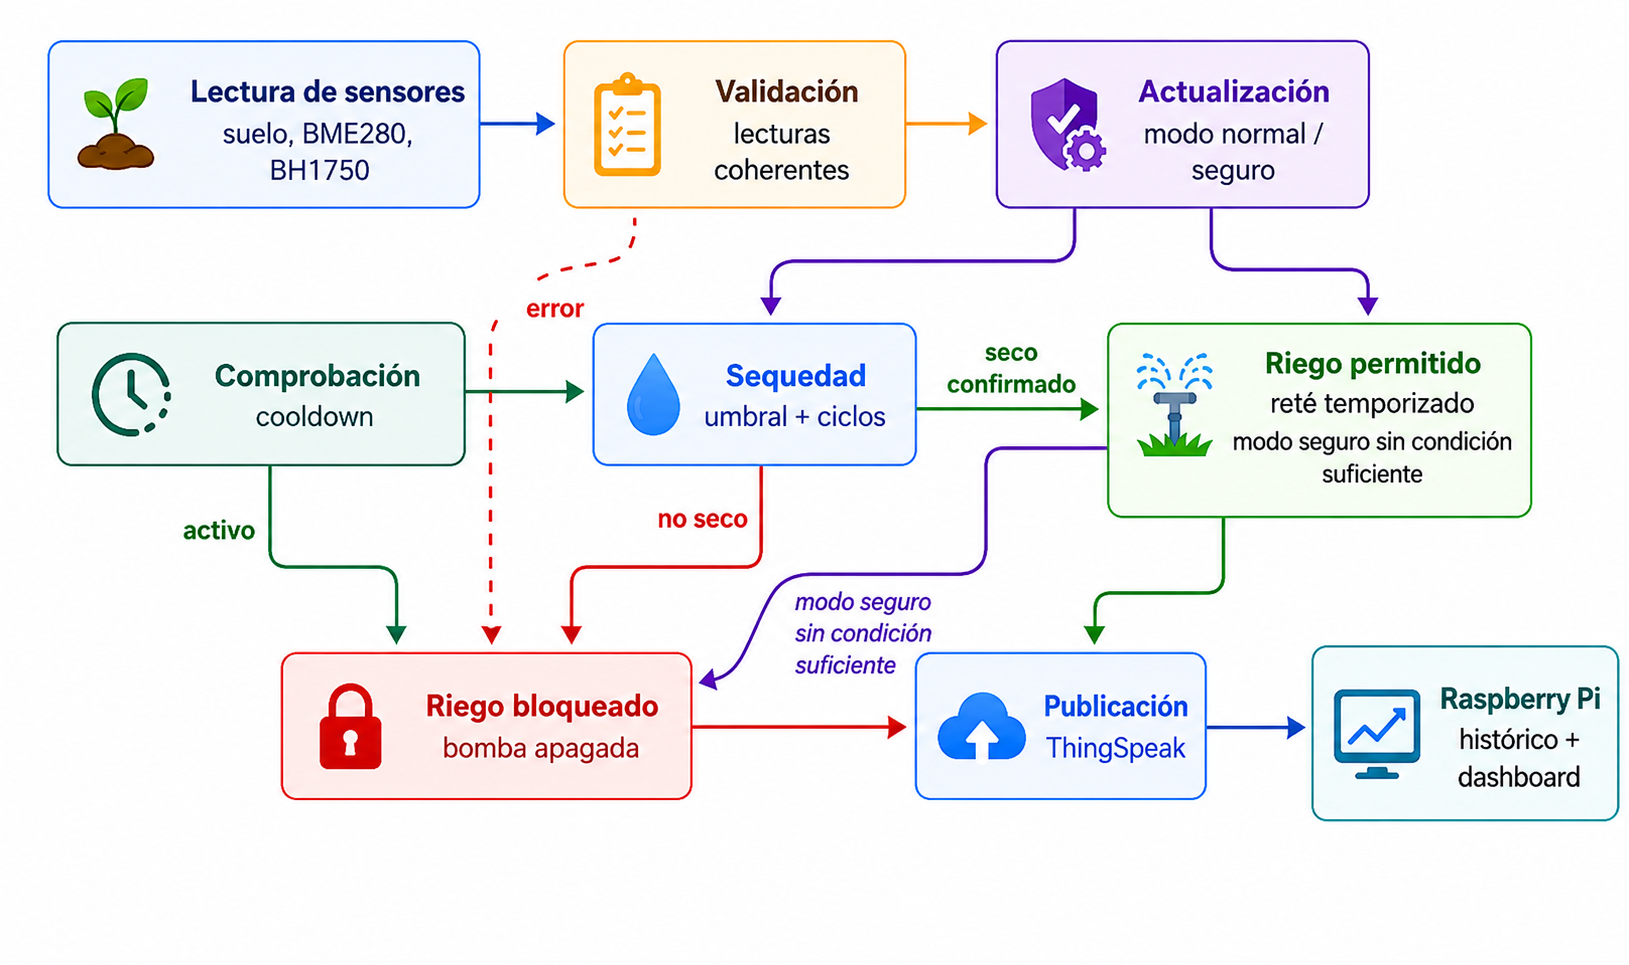
\includegraphics[width=\textwidth]{figs_png/motor_reglas_flujo.png}
\caption{Flujo lógico simplificado de la lógica local de decisión. La estación decide localmente y la Raspberry Pi supervisa el resultado publicado.}
\label{fig:cap6_motor_reglas_flujo}
\end{figure}

El primer filtro de la lógica de decisión es la validez de los sensores. Una lectura ausente, incoherente o no inicializada no debe activar la bomba. Si el firmware detecta un problema en las medidas necesarias para decidir, el sistema adopta una respuesta conservadora: no riega, mantiene el relé apagado y publica el código \texttt{400}. Este código permite que la Raspberry Pi y el dashboard distingan un estado de error de una situación normal sin riego.

El segundo elemento es el modo de funcionamiento. En modo normal, la estación evalúa si la humedad del suelo está por debajo del umbral configurado y si esa condición se mantiene durante los ciclos necesarios. En modo seguro, la estación se comporta de forma más restrictiva: no basta con una lectura puntual de sequedad, sino que se exige una condición más clara antes de permitir la actuación. Si el sistema se encuentra en modo seguro y no se autoriza el riego, se publica el código \texttt{206}.

El tercer elemento es el cooldown. Después de una actuación, la estación espera un tiempo mínimo antes de permitir otro riego. Esta regla evita activaciones repetidas por lecturas inestables o por la lenta estabilización del sensor después de aportar agua. En pruebas de demostración este valor puede configurarse con una duración reducida, por ejemplo decenas de segundos, mientras que en una instalación real debería utilizarse un valor más conservador. Si el cooldown está activo, el sistema no riega y publica el código \texttt{429}.

La decisión de riego se basa principalmente en la humedad del suelo. En la versión actual del firmware, la estación compara el porcentaje de humedad con un umbral normal o con un umbral de modo seguro, según el estado interno. Además, mantiene un contador de ciclos secos consecutivos. Esta confirmación por ciclos evita que una única lectura anómala active la bomba. La Figura~\ref{fig:cap6_confirmacion_humedad} representa esta lógica de forma simplificada.

\begin{figure}[H]
\centering
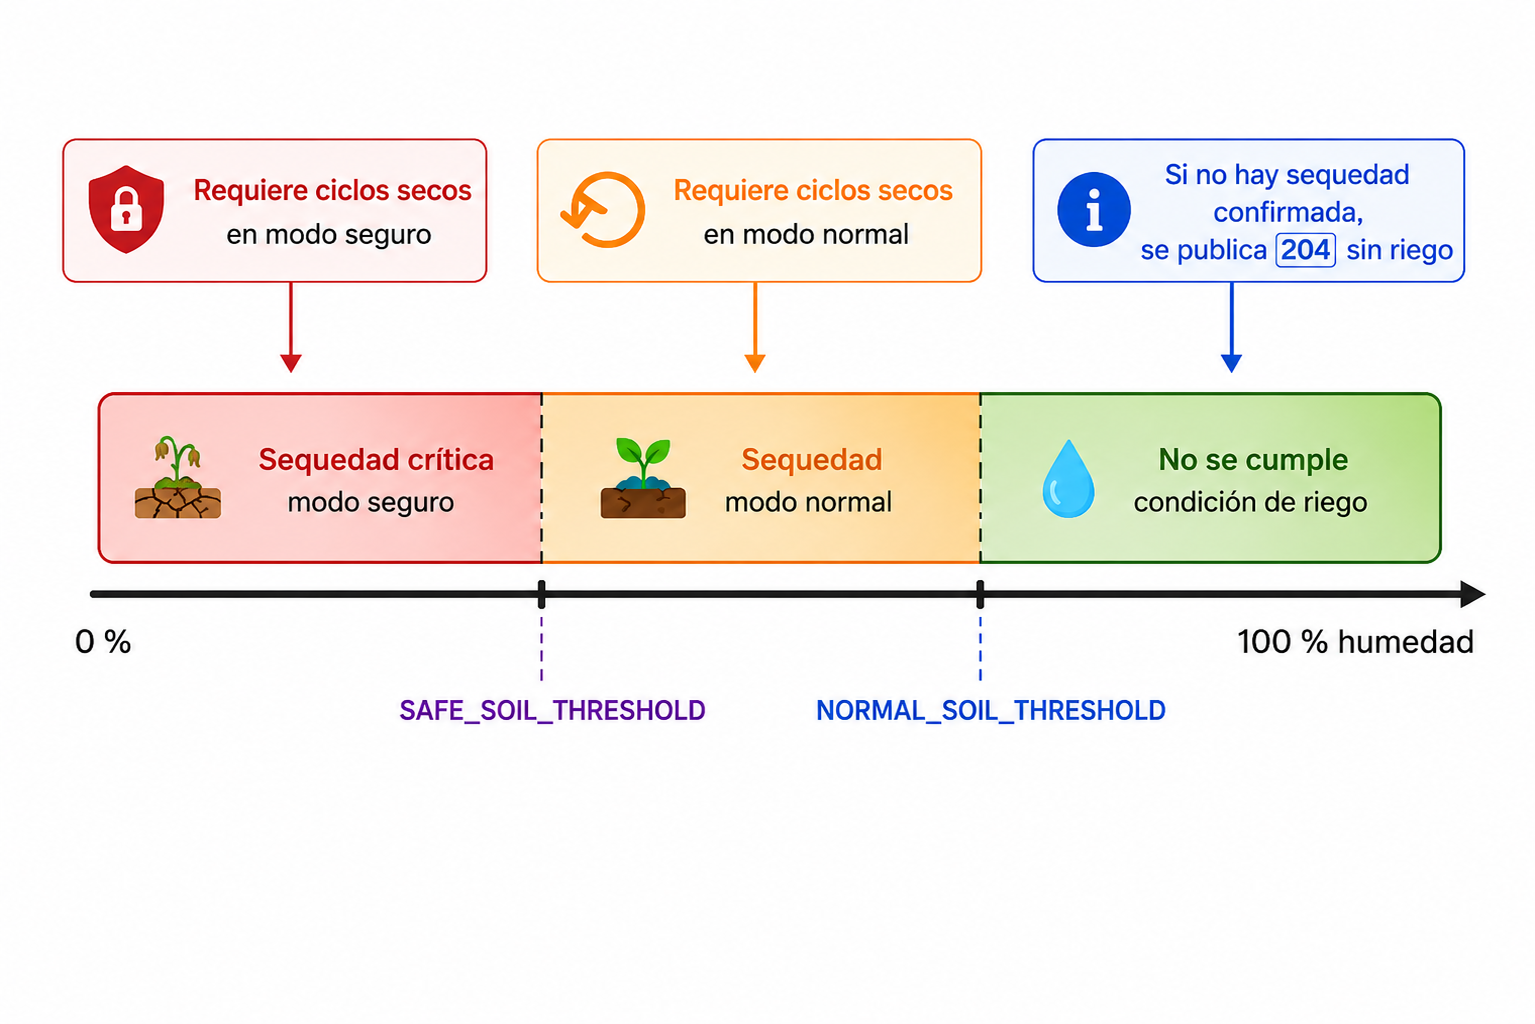
\includegraphics[width=\textwidth]{figs_png/cap6_confirmacion_humedad.png}
\caption{Confirmación de sequedad mediante umbrales y ciclos consecutivos. El modo seguro utiliza una condición más restrictiva que el modo normal.}
\label{fig:cap6_confirmacion_humedad}
\end{figure}

En este contexto, la histéresis no se implementa como un control continuo que mantenga la bomba encendida hasta alcanzar otro umbral. Esto sería menos seguro para el prototipo, porque dependería de que el sensor reaccionase inmediatamente al riego. En TierraViva, la histéresis se aplica de forma práctica mediante tres mecanismos: confirmación por ciclos secos, separación entre umbral normal y umbral de modo seguro, y cooldown después de cada actuación. Así se evita que pequeñas oscilaciones alrededor del umbral provoquen riegos repetidos o cambios de estado demasiado frecuentes.

Cuando el riego se autoriza, la bomba no queda activa indefinidamente. La actuación se ejecuta mediante una función temporizada: se activa el relé, se espera la duración configurada y se desactiva siempre al finalizar. Este comportamiento es esencial porque el apagado de la bomba no depende de la Raspberry Pi, del dashboard ni de una nueva lectura de ThingSpeak. La estación cierra localmente el ciclo de actuación.

La Tabla~\ref{cuadro:cap6_codigos_motor} resume los códigos actuales publicados por la estación. Estos códigos son los que deben interpretarse desde la Raspberry Pi y el dashboard para mostrar el estado operativo de cada estación.

\begin{table}[H]
\centering
\small
\begin{tabular}{|p{0.16\textwidth}|p{0.28\textwidth}|p{0.46\textwidth}|}
\hline
\textbf{Código} & \textbf{Estado} & \textbf{Interpretación} \\
\hline
\texttt{200} & Riego ejecutado / OK & La estación ha autorizado y completado una actuación de riego temporizada. \\
\hline
\texttt{204} & Sin riego & Las lecturas son válidas, pero no se cumple la condición de sequedad confirmada. \\
\hline
\texttt{206} & Modo seguro & La estación se encuentra en modo conservador y no autoriza riego salvo condición suficientemente clara. \\
\hline
\texttt{400} & Error de sensores & Una lectura necesaria no es válida o algún sensor crítico no responde correctamente. \\
\hline
\texttt{429} & Cooldown & Se bloquea una nueva actuación porque no ha transcurrido el tiempo mínimo desde el último riego. \\
\hline
\end{tabular}
\caption{Códigos actuales publicados por la estación.}
\label{cuadro:cap6_codigos_motor}
\end{table}

La lógica principal puede resumirse mediante el fragmento del Código~\ref{cod:motor_reglas_decision}. No se incluye el sketch completo, sino la parte esencial de la decisión. El orden de comprobación es relevante: primero se descartan errores de sensores, después se comprueba el cooldown, y solo entonces se evalúa la sequedad según el modo normal o seguro.

\begin{code}[H]
\begin{lstlisting}[language=C++]
bool shouldIrrigate() {
  if (!sensorOk) {
    statusCode = 400;       // Error de sensores
    return false;
  }

  if (cooldownActive()) {
    statusCode = 429;       // Cooldown activo
    return false;
  }

  if (safeMode) {
    return (soilPercent <= SAFE_SOIL_THRESHOLD) &&
           (dryCycleCount >= SAFE_CONFIRM_DRY_CYCLES);
  }

  return (soilPercent <= NORMAL_SOIL_THRESHOLD) &&
         (dryCycleCount >= NORMAL_CONFIRM_DRY_CYCLES);
}
\end{lstlisting}
\caption{Resumen de la decisión local de riego}
\label{cod:motor_reglas_decision}
\end{code}

El código anterior no asigna por sí solo todos los estados finales. Cuando \texttt{shouldIrrigate()} devuelve \texttt{true}, el bucle principal ejecuta el riego temporizado y publica \texttt{200}. Cuando devuelve \texttt{false}, el firmware distingue la causa: error de sensores, cooldown, modo seguro o ausencia de necesidad de riego. Esta separación permite que el dashboard no muestre simplemente ``riego/no riego'', sino el motivo de la decisión.

\begin{code}[H]
\begin{lstlisting}[language=C++]
readSensors();
updateSafetyState();

if (shouldIrrigate()) {
  irrigateForSeconds(IRRIGATION_SECONDS);
  statusCode = 200;      // Riego ejecutado
} else {
  if (!sensorOk) {
    statusCode = 400;    // Error de sensores
  } else if (cooldownActive()) {
    statusCode = 429;    // Cooldown activo
  } else if (safeMode) {
    statusCode = 206;    // Modo seguro
  } else {
    statusCode = 204;    // Sin riego
  }
}

sendThingSpeak();
\end{lstlisting}
\caption{Asignación del código operativo antes de publicar en ThingSpeak}
\label{cod:asignacion_codigos_motor}
\end{code}

La actuación sobre el relé se limita temporalmente. El firmware activa la salida de control, espera el número de segundos configurado y después apaga el relé. En el montaje real, esta salida controla el módulo de relé que alimenta la bomba de agua de 12 V. La decisión de apagar el relé desde el propio firmware reduce el riesgo de riego indefinido ante fallos de comunicación o pérdida de supervisión.

\begin{code}[H]
\begin{lstlisting}[language=C++]
void irrigateForSeconds(unsigned long seconds) {
  relayActive = true;
  digitalWrite(RELAY_PIN, RELAY_ON);

  delay(seconds * 1000UL);

  digitalWrite(RELAY_PIN, RELAY_OFF);
  relayActive = false;
  lastIrrigationEndMs = millis();
}
\end{lstlisting}
\caption{Actuación temporizada sobre el relé}
\label{cod:riego_temporizado}
\end{code}

El resultado de cada ciclo se publica en ThingSpeak junto con la telemetría. Los campos de sensores permiten interpretar el contexto físico de la estación, mientras que el estado del relé y el código operativo permiten conocer el resultado de la decisión. La Raspberry Pi consulta posteriormente esos datos, los almacena en SQLite y los expone al dashboard, pero no modifica la decisión local tomada por la estación.

Este diseño hace que la lógica local sea simple, verificable y seguro. Simple, porque utiliza condiciones explícitas y parámetros configurables. Verificable, porque cada salida puede relacionarse con un código concreto publicado en ThingSpeak. Y seguro, porque ante lecturas inválidas, cooldown activo o modo seguro no confirmado, la respuesta por defecto es mantener la bomba apagada. De este modo, TierraViva cierra localmente el ciclo medir--decidir--actuar, mientras que la Raspberry Pi conserva el papel de supervisión e histórico.

\section{API FastAPI}
\label{sec:api_fastapi}

La API de TierraViva constituye la capa de servicio entre la base de datos local y el dashboard web. Su función no es comunicarse directamente con las estaciones ni decidir el riego, sino ofrecer una interfaz HTTP para consultar de forma estructurada la información ya almacenada en la Raspberry Pi. De este modo, el frontend no necesita acceder directamente a SQLite ni conocer los detalles internos del módulo de ingesta.

\begin{wrapfigure}{r}{0.32\textwidth}
    \vspace{-12pt}
    \centering
    
\includegraphics[width=0.30\textwidth]{figs/fast_api_logo.png}
    \caption{Logo FastAPI}
    \label{fig:logo_fastapi}
    \vspace{-8pt}
\end{wrapfigure}

La implementación se realiza con FastAPI, un framework Python orientado a la creación de APIs web. En el contexto de TierraViva, FastAPI permite definir endpoints claros, validar parámetros de consulta y devolver respuestas en formato JSON. Esta elección mantiene el código compacto, facilita la depuración y ofrece una documentación automática de la API durante la ejecución del servidor.

La API se ejecuta mediante Uvicorn, escuchando en el puerto \texttt{8000}. El script de gestión \texttt{tierraviva.sh} arranca por separado el proceso de ingesta y el servidor web, de modo que la lectura de ThingSpeak y la consulta desde el dashboard quedan desacopladas. Si el dashboard realiza varias peticiones seguidas, estas se atienden desde la base de datos local, sin forzar una consulta nueva a ThingSpeak en cada refresco de pantalla.

La Figura~\ref{fig:cap6_api_flujo} resume el papel de la API dentro del software de la Raspberry Pi.

\begin{figure}[H]
\centering
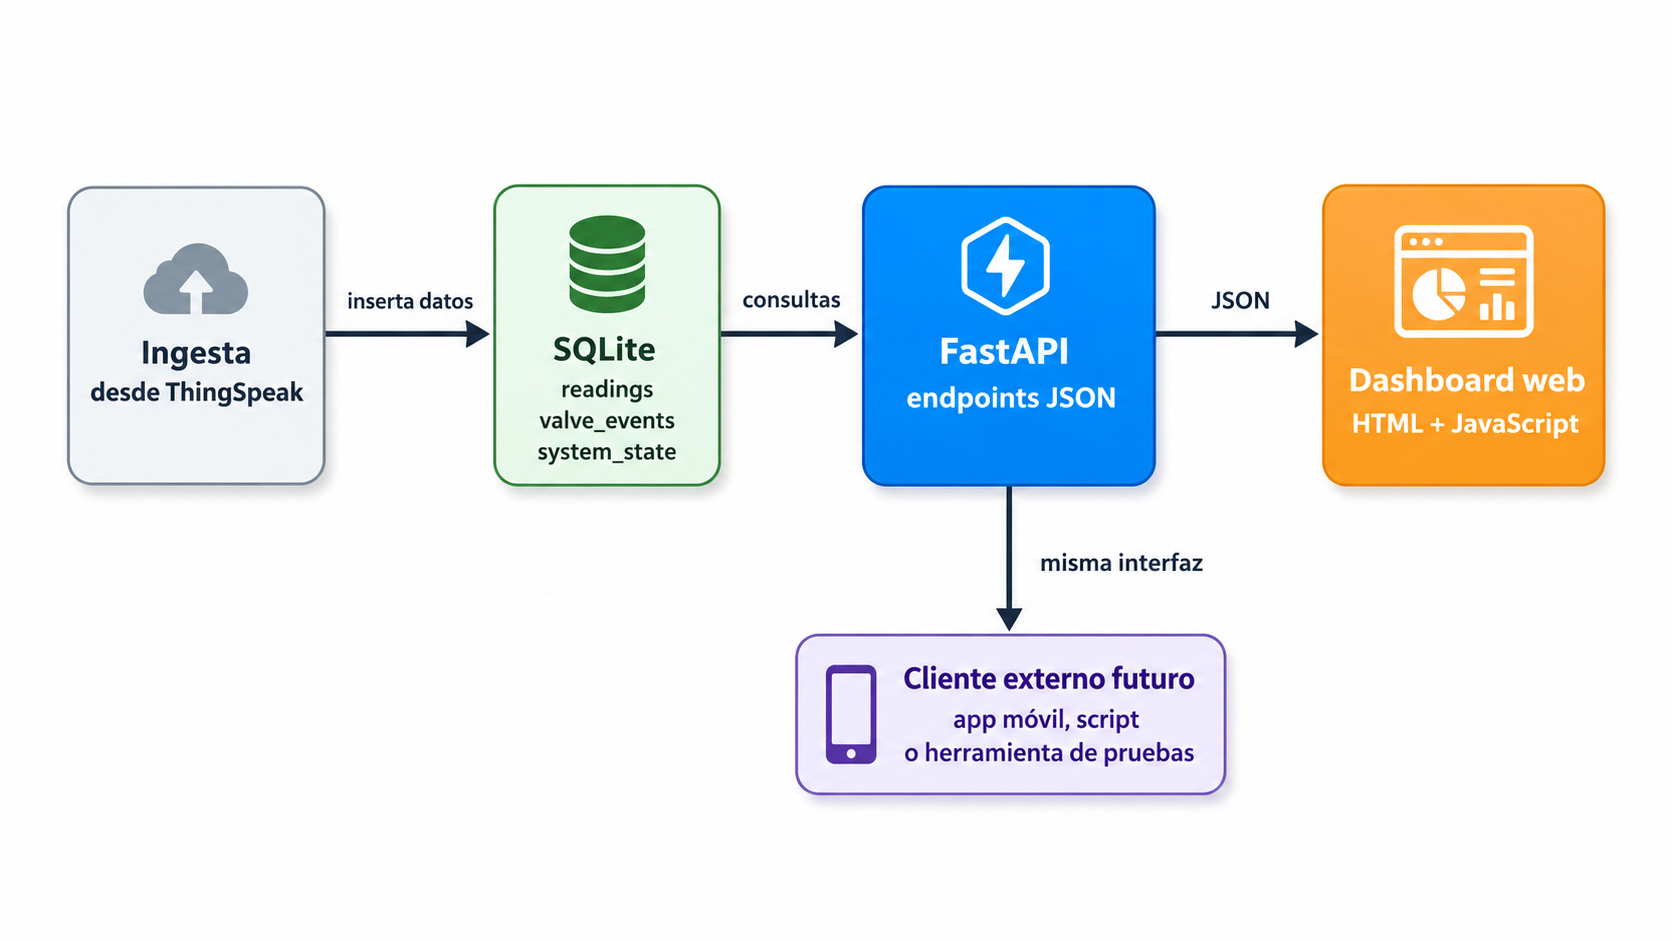
\includegraphics[width=0.80\textwidth]{figs_png/api_flujo.png}
\caption{Papel de FastAPI como capa de servicio entre SQLite y los clientes de consulta.}
\label{fig:cap6_api_flujo}
\end{figure}

El diseño de la API sigue una separación de responsabilidades sencilla. El módulo \texttt{database.py} conserva las funciones de acceso a datos; \texttt{api.py} se limita a validar parámetros, llamar a esas funciones y enriquecer algunas respuestas con información útil para la interfaz. Por ejemplo, una lectura puede completarse con su antigüedad en segundos, una etiqueta de frescura y una clasificación del estado del suelo.

La Tabla~\ref{cuadro:cap6_endpoints_api} resume los endpoints principales de la API. 

\begin{table}[H]
\centering
\small
\setlength{\tabcolsep}{4pt}
\renewcommand{\arraystretch}{1.1}
\begin{tabular}{|p{0.27\textwidth}|p{0.15\textwidth}|p{0.48\textwidth}|}
\hline
\textbf{Endpoint} & \textbf{Método} & \textbf{Función principal} \\
\hline
\texttt{/} & GET & Sirve el fichero \texttt{index.html} del dashboard. \\
\hline
\texttt{/api/config} & GET & Devuelve la configuración general del sistema: estación seleccionada, estaciones activas, umbrales, ruta de base de datos y últimas marcas de ingesta. \\
\hline
\texttt{/api/latest} & GET & Devuelve la última lectura almacenada para una estación, junto con antigüedad, frescura y estado interpretado del suelo. \\
\hline
\texttt{/api/readings} & GET & Devuelve el histórico reciente de lecturas de una estación, con un límite configurable de muestras. \\
\hline
\texttt{/api/stats} & GET & Calcula estadísticas agregadas para una ventana temporal configurable. \\
\hline
\texttt{/api/health} & GET & Comprueba el estado básico del servicio: base de datos, frontend y disponibilidad de lecturas. \\
\hline
\end{tabular}
\caption{Endpoints implementados en la API FastAPI}
\label{cuadro:cap6_endpoints_api}
\end{table}

El endpoint \texttt{/api/latest} se utiliza para obtener la situación más reciente de una estación. Recibe como parámetro el identificador de estación, por ejemplo \texttt{station=A}, y devuelve la última lectura almacenada. Además de los datos originales, la API calcula campos derivados como \texttt{age\_seconds}, \texttt{freshness} y \texttt{soil\_state}. Estos campos evitan que el dashboard tenga que repetir lógica de interpretación en JavaScript.

\begin{lstlisting}[language=Python, caption={Esquema simplificado del endpoint de última lectura}, label={cod:api_latest}]
@app.get("/api/latest")
def api_latest(station: Optional[str] = Query(None)):
    selected_station = normalize_station(station)
    reading = get_latest_reading(selected_station)

    if reading is None:
        return {
            "ok": False,
            "station": selected_station,
            "reading": None,
            "status": "sin_datos",
        }

    age_seconds = age_seconds_from_ts(reading["ts"])
    soil = reading.get("soil_moisture_pct")

    return {
        "ok": True,
        "station": selected_station,
        "reading": reading,
        "age_seconds": age_seconds,
        "freshness": freshness_label(age_seconds),
        "soil_state": soil_label(soil),
    }
\end{lstlisting}

El endpoint \texttt{/api/readings} expone el histórico reciente. Su parámetro \texttt{limit} permite controlar cuántas muestras se devuelven, con límites internos para evitar respuestas excesivamente grandes. Esta consulta es la base de las gráficas temporales del dashboard, ya que permite recuperar las últimas medidas de humedad del suelo, temperatura, humedad relativa, luminosidad y presión.

El endpoint \texttt{/api/stats} proporciona un resumen agregado para una ventana temporal expresada en horas. Con \texttt{hours=24} se obtiene un resumen diario; con \texttt{hours=168}, un resumen semanal. Esta decisión evita crear endpoints separados para día y semana, y permite reutilizar la misma función para diferentes escalas temporales. El resultado puede incluir valores medios, mínimos y máximos de las principales magnitudes registradas.

\begin{table}[H]
\centering
\small
\begin{tabular}{|p{0.30\textwidth}|p{0.25\textwidth}|p{0.35\textwidth}|}
\hline
\textbf{Consulta} & \textbf{Ejemplo} & \textbf{Uso en el sistema} \\
\hline
Última lectura de A & \texttt{/api/latest?station=A} & Tarjetas principales del dashboard. \\
\hline
Histórico reciente de B & \texttt{/api/readings?station=B\&limit=120} & Gráficas de evolución temporal. \\
\hline
Resumen diario & \texttt{/api/stats?station=A\&hours=24} & Valores medios, mínimos y máximos del último día. \\
\hline
Resumen semanal & \texttt{/api/stats?station=A\&hours=168} & Análisis de tendencia semanal. \\
\hline
Consulta de salud & \texttt{/api/health?station=A} & Diagnóstico básico del servicio, disponibilidad de datos y existencia del frontend. \\
\hline
Configuración de A & \texttt{/api/config?station=A} & Consulta de umbrales, estación activa, rutas locales y última ingesta registrada. \\
\hline
\end{tabular}
\caption{Ejemplos de consulta a la API}
\label{cuadro:cap6_consultas_api}
\end{table}

La API pública se mantiene deliberadamente centrada en la consulta de lecturas, configuración, estadísticas y diagnóstico. Aunque la base de datos contiene una tabla preparada para eventos operativos, la versión actual del backend no expone endpoints de control ni de envío de órdenes hacia las estaciones. Esta decisión mantiene la coherencia con la arquitectura final: la Raspberry Pi consulta y muestra información, pero no participa en la actuación física sobre el riego.

Desde el punto de vista del dashboard, esta API permite construir una interfaz reactiva sin acoplarla a la base de datos. La web puede solicitar periódicamente \texttt{/api/latest}, \texttt{/api/readings} y \texttt{/api/stats}; si una estación deja de actualizarse, la antigüedad de la última lectura permite mostrar un estado \textit{fresh}, \textit{stale} u \textit{offline}. Esta lógica mejora la interpretación visual: no basta con enseñar el último valor recibido, también es necesario indicar si ese valor sigue siendo reciente.

El endpoint \texttt{/api/health} se reserva para diagnóstico. Devuelve información básica sobre el servicio, como la existencia del frontend, la ruta de la base de datos y si hay datos disponibles para alguna estación. Este tipo de endpoint es útil durante la instalación en Raspberry Pi, porque permite comprobar rápidamente si el servidor está levantado y si la API puede acceder a la información local.

En conjunto, FastAPI actúa como una frontera clara entre almacenamiento y visualización. La base de datos conserva el histórico; la API lo transforma en respuestas JSON coherentes; y el dashboard consume esas respuestas sin conocer la estructura interna de SQLite. Esta separación hace que el software sea más mantenible y deja abierta la posibilidad de añadir otros clientes en el futuro, como una aplicación móvil, una herramienta de análisis o scripts de validación, reutilizando la misma interfaz HTTP.

\section{Dashboard web de supervisión}
\label{sec:dashboard_web_supervision}

El último bloque software de la Raspberry Pi es el dashboard web de supervisión. Su función es presentar al usuario la información almacenada y servida por la API de forma comprensible, sin obligarle a consultar directamente ThingSpeak, SQLite o los logs del sistema. El dashboard no participa en la decisión de riego ni envía órdenes a las estaciones; actúa como interfaz de visualización del estado publicado por los nodos de campo.

La interfaz principal se define en el fichero \texttt{dashboard/index.html}, mientras que la lógica de actualización se implementa en \texttt{dashboard/js/tierraviva.js}. El fichero HTML contiene la estructura visual del panel: cabecera, selector de estación, tarjetas de lectura actual, gráficas, resumen histórico y tabla de últimas lecturas. El fichero JavaScript se encarga de consultar periódicamente la API, interpretar las respuestas y actualizar los elementos de la página.

El dashboard está organizado alrededor de una estación seleccionada. En la versión actual se contemplan las estaciones \texttt{A} y \texttt{B}, y el usuario puede alternar entre ellas mediante un selector. Esta decisión mantiene la coherencia con la arquitectura multiestación del sistema: la misma interfaz puede mostrar datos de distintas zonas sin duplicar el código del frontend.

La Tabla~\ref{cuadro:cap6_campos_dashboard} resume los principales campos mostrados en el dashboard.

\begin{table}[H]
\centering
\small
\begin{tabular}{|p{0.28\textwidth}|p{0.30\textwidth}|p{0.32\textwidth}|}
\hline
\textbf{Elemento mostrado} & \textbf{Origen en la API} & \textbf{Interpretación} \\
\hline
Humedad del suelo & \texttt{soil\_moisture\_pct} & Valor normalizado de humedad utilizado para clasificar el suelo como seco, normal o húmedo. \\
\hline
Temperatura & \texttt{temperature\_c} & Temperatura ambiente medida por la estación. \\
\hline
Humedad ambiental & \texttt{humidity\_pct} & Humedad relativa del aire. \\
\hline
Luminosidad & \texttt{light\_lux} & Nivel de luz ambiente medido en lux. \\
\hline
Presión & \texttt{pressure\_hpa} & Presión atmosférica medida por el sensor ambiental. \\
\hline
Última lectura & \texttt{ts}, \texttt{age\_seconds}, \texttt{freshness} & Información temporal para saber si los datos son recientes, antiguos u obsoletos. \\
\hline
Estado del relé & \texttt{relay\_state} & Indica si el bloque de actuación aparece como apagado o activo según la última publicación. \\
\hline
Estado/evento & \texttt{system\_event} & Estado operativo publicado por la estación. \\
\hline
Debug/código & \texttt{debug\_code} & Código auxiliar de diagnóstico o estado publicado por la estación. \\
\hline
\end{tabular}
\caption{Campos principales mostrados en el dashboard web}
\label{cuadro:cap6_campos_dashboard}
\end{table}

La pantalla inicial muestra tarjetas con las magnitudes más recientes: humedad del suelo, temperatura, humedad ambiental, luminosidad y presión. Estas tarjetas permiten comprobar rápidamente el estado de la estación seleccionada. Además, el panel incluye información de actualización, mostrando si la última lectura se considera reciente, retrasada u obsoleta. Esta distinción es importante porque un valor aparentemente correcto puede no ser útil si la estación lleva demasiado tiempo sin publicar datos nuevos.

El dashboard también interpreta la humedad del suelo mediante umbrales configurados. En lugar de mostrar únicamente un número, el frontend clasifica el valor como \textit{seco}, \textit{normal} o \textit{húmedo}. Esta interpretación se realiza a partir de los umbrales recibidos desde \texttt{/api/config}. De esta forma, la interfaz puede adaptarse a cambios de configuración sin modificar manualmente el código HTML.

La actualización de datos se realiza mediante peticiones HTTP periódicas a la API. El script \texttt{tierraviva.js} consulta los endpoints \texttt{/api/config}, \texttt{/api/latest}, \texttt{/api/readings} y \texttt{/api/stats} para obtener configuración, última lectura, histórico reciente y resumen estadístico. Estas peticiones se realizan para la estación seleccionada, utilizando el parámetro \texttt{station}. El intervalo de refresco se obtiene de la configuración del sistema mediante \texttt{web\_refresh\_seconds}; si no está disponible, se utiliza un valor por defecto de tres segundos.

\begin{table}[H]
\centering
\small
\begin{tabular}{|p{0.42\textwidth}|p{0.50\textwidth}|}
\hline
\textbf{Consulta realizada por el dashboard} & \textbf{Uso en la interfaz} \\
\hline
\texttt{/api/config?station=A} & Obtener estación activa, lista de estaciones, umbrales y periodo de refresco. \\
\hline
\texttt{/api/latest?station=A} & Actualizar las tarjetas principales con la última lectura disponible. \\
\hline
\texttt{/api/readings?station=A\&limit=10} & Construir gráficas y tabla de lecturas recientes. \\
\hline
\texttt{/api/stats?station=A\&hours=24} & Mostrar el resumen histórico de las últimas 24 horas. \\
\hline
\end{tabular}
\caption{Consultas principales realizadas por el dashboard a la API}
\label{cuadro:cap6_consultas_dashboard}
\end{table}

Además de las tarjetas principales, el dashboard incorpora gráficas de evolución temporal. Estas gráficas permiten observar la tendencia reciente de las variables ambientales y de suelo, en lugar de analizar únicamente la última muestra recibida. Esta visualización resulta útil durante las pruebas porque permite detectar comportamientos anómalos, valores constantes, saltos bruscos o ausencia de actualización.

El panel incluye también un resumen histórico de las últimas 24 horas. Este resumen calcula valores agregados, como medias, mínimos y máximos, a partir de los datos devueltos por la API. En el caso de los campos operativos, como el estado del relé, el estado/evento y el código de depuración, el dashboard muestra información de frecuencia o último valor disponible. Así, el usuario puede distinguir no solo las condiciones ambientales, sino también el comportamiento operativo reciente de la estación.

La tabla de últimas lecturas completa la visualización. En ella se muestran varias muestras recientes con fecha, humedad del suelo, temperatura, humedad relativa, luminosidad y presión. Esta tabla resulta especialmente útil durante la depuración, ya que permite comprobar si las lecturas se insertan en orden, si aparecen valores nulos o si la evolución de los datos es coherente con lo mostrado en las tarjetas y gráficas.

Desde el punto de vista de diseño, el dashboard se mantiene como una capa de presentación. No accede directamente a ThingSpeak ni a SQLite, sino que consume exclusivamente la API expuesta por FastAPI. Esta separación evita duplicar lógica de acceso a datos en el frontend y facilita que los cambios en la base de datos o en la ingesta no obliguen a modificar la estructura visual, siempre que la API mantenga el contrato de respuesta.

En caso de error, ausencia de datos o pérdida de actualización, el dashboard no debe ocultar la situación. Si la API no devuelve una lectura válida, la interfaz muestra valores vacíos o mensajes de espera. Si la lectura existe pero es antigua, el estado de frescura permite indicar que la estación no se está actualizando correctamente. Esta forma de visualización es importante en TierraViva porque la supervisión no consiste solo en mostrar números, sino en informar de si esos números siguen siendo fiables.

En conjunto, el dashboard web convierte los datos técnicos del sistema en una vista útil para el usuario. Las estaciones siguen siendo responsables de medir, decidir y actuar localmente; la Raspberry conserva el histórico y sirve la API; y el dashboard permite supervisar el estado del sistema sin intervenir en la actuación física. Con ello se cierra el flujo software de TierraViva: ingesta desde ThingSpeak, almacenamiento en SQLite, exposición mediante FastAPI y visualización web.

\section{Ejecución y gestión del sistema software}
\label{sec:ejecucion_gestion_software}

Para facilitar la puesta en marcha del software en la Raspberry Pi, el proyecto incluye el script \texttt{tierraviva.sh}. Este script agrupa las operaciones principales de despliegue y ejecución, evitando tener que lanzar manualmente cada componente desde la terminal.

El script permite instalar dependencias, preparar el entorno virtual, copiar el dashboard al directorio esperado por FastAPI, arrancar el proceso de ingesta \texttt{main.py}, iniciar el servidor \texttt{api.py} mediante Uvicorn, consultar el estado de ejecución, detener los procesos y revisar los logs. Esta automatización resulta útil durante las pruebas porque reduce errores repetitivos de arranque y deja una forma reproducible de iniciar el sistema.

\begin{table}[H]
\centering
\small
\begin{tabular}{|p{0.25\textwidth}|p{0.60\textwidth}|}
\hline
\textbf{Comando} & \textbf{Función} \\
\hline
\texttt{./tierraviva.sh install} & Crea el entorno, instala dependencias e inicializa la base de datos. \\
\hline
\texttt{./tierraviva.sh start} & Arranca el proceso de ingesta y el servidor de la API, mostrando los logs. \\
\hline
\texttt{./tierraviva.sh stop} & Detiene los procesos asociados al sistema. \\
\hline
\texttt{./tierraviva.sh restart} & Reinicia los servicios del prototipo. \\
\hline
\texttt{./tierraviva.sh status} & Muestra si \texttt{main.py} y \texttt{api.py} están en ejecución. \\
\hline
\texttt{./tierraviva.sh logs} & Muestra las últimas líneas de log generadas por los procesos. \\
\hline
\end{tabular}
\caption{Operaciones principales del script de gestión \texttt{tierraviva.sh}}
\label{cuadro:cap6_tierraviva_sh}
\end{table}

Además de arrancar los procesos, el script carga el fichero \texttt{.env} cuando está disponible. Esto permite mantener fuera del código fuente las claves de ThingSpeak y los identificadores de canal. Durante el arranque, el script comprueba que existen las variables necesarias para consultar las estaciones configuradas, como los identificadores de canal y las claves de lectura de ThingSpeak. Si faltan identificadores de canal o claves de lectura, el proceso de ingesta no continúa como si el sistema estuviera correctamente configurado, sino que deja el error reflejado en los logs.

Esta capa de gestión no modifica la arquitectura del sistema: la estación sigue siendo autónoma y la Raspberry mantiene un papel de supervisión. Su valor está en hacer que el backend sea más reproducible, más fácil de ejecutar y más sencillo de depurar durante las pruebas.



\chapter{Validación y pruebas}
\label{cap:validacion_pruebas}

Una vez implementadas las estaciones de campo y el sistema de supervisión en Raspberry Pi, se ha realizado una validación progresiva del prototipo TierraViva.

Además de las pruebas de laboratorio y de integración controlada, se incluye una prueba funcional en entorno real en Agrolab Móstoles, situado en Móstoles, Madrid. Agrolab se utiliza como entorno de validación por tratarse de un espacio de agricultura urbana/periurbana, más próximo al contexto de uso previsto que el montaje inicial de laboratorio \cite{ayto_mostoles_agrolab_2020}. Esta prueba permite comprobar el comportamiento del prototipo en una zona de cultivo real y obtener evidencia audiovisual del funcionamiento de la estación, la publicación de datos y la actuación controlada del riego.

El plan completo de pruebas, criterios de aceptación y relación con riesgos técnicos, se recoge en el Anexo~\ref{anexo:plan_pruebas}. La relación entre requisitos, pruebas y evidencias se documenta de forma complementaria en el Anexo~\ref{anexo:trazabilidad_requisitos_pruebas}. En este capítulo se presenta únicamente la síntesis de validación necesaria para evaluar el funcionamiento global del prototipo.

\section{Estrategia de validación}
\label{sec:estrategia_validacion}

La validación se ha organizado de forma incremental, desde componentes aislados hasta el flujo completo extremo a extremo. Esta estrategia evita que los errores de alimentación, cableado, comunicación o software aparezcan únicamente al final, cuando resulta más difícil aislar su origen. La Figura~\ref{fig:estrategia_incremental_validacion} resume los niveles aplicados.

\begin{figure}[H]
    \centering
    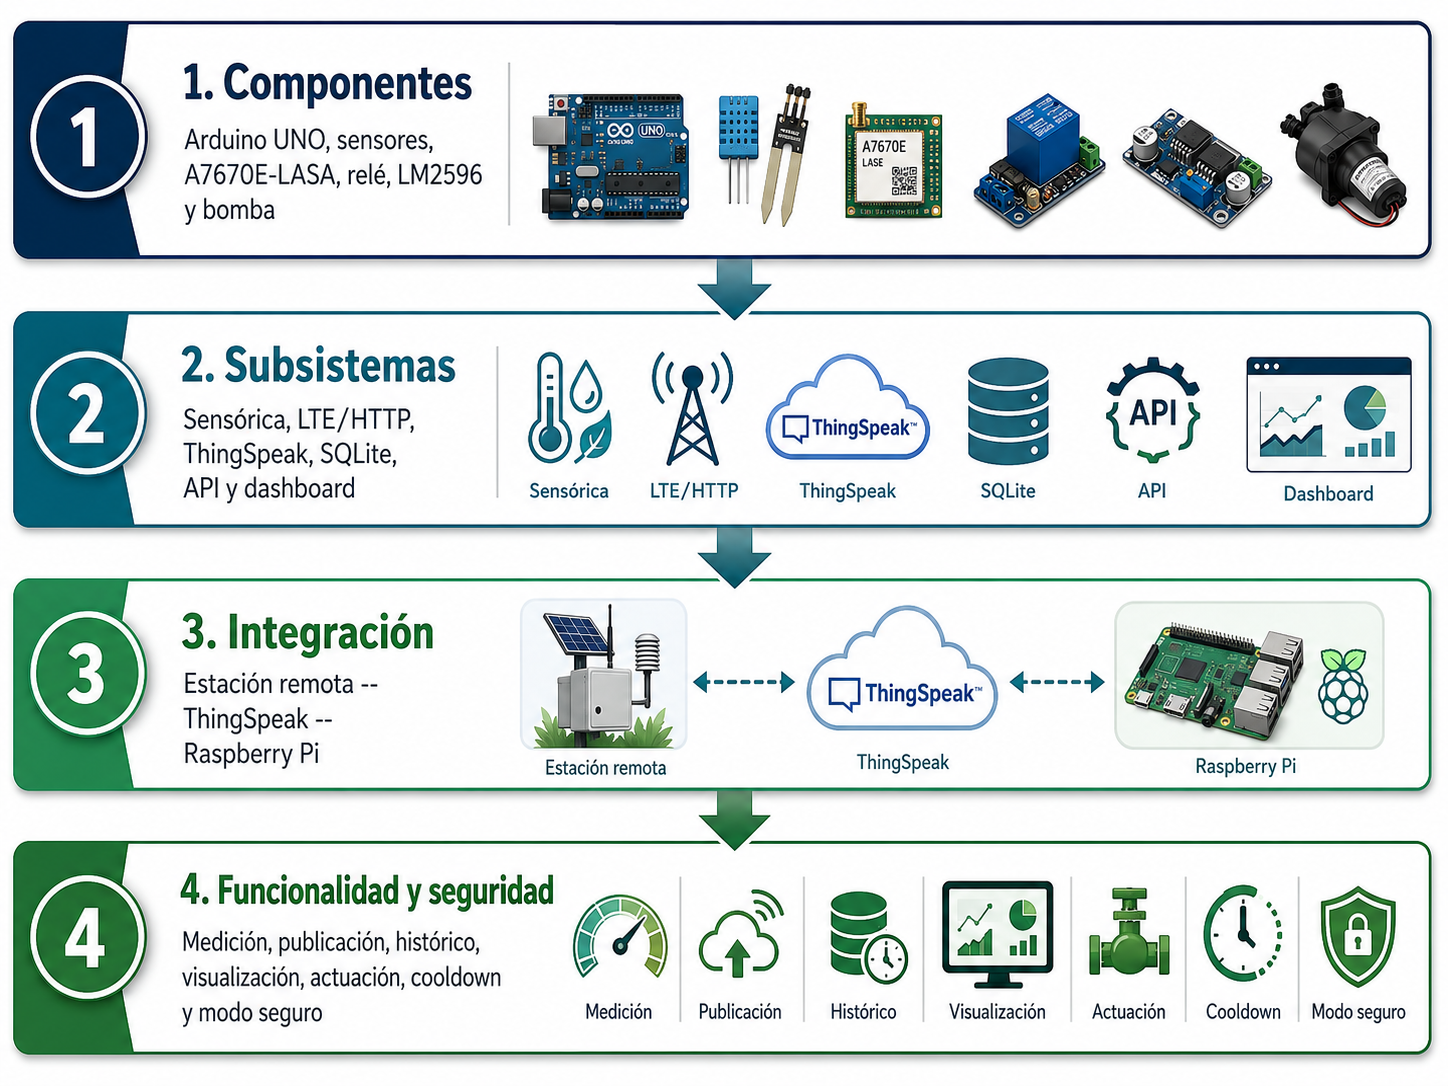
\includegraphics[width=\textwidth]{figs_png/estrategia_incremental_validacion.png}
    \caption{Estrategia incremental de validación aplicada en TierraViva. Elaboración propia, véase Anexo~\ref{sec:uso_ia_generativa_tfg}.}
    \label{fig:estrategia_incremental_validacion}
\end{figure}

La validación se interpreta como una comprobación técnica del prototipo desarrollado. El objetivo es demostrar que la arquitectura propuesta funciona, que los bloques se comunican correctamente y que la actuación sobre el riego incorpora medidas básicas de seguridad.

\section{Resumen de pruebas realizadas}
\label{sec:resumen_pruebas_realizadas}

La Tabla~\ref{tab:cap7_resumen_pruebas} resume las pruebas principales ejecutadas durante la validación. Se han agrupado siguiendo la numeración definida en el Anexo~\ref{anexo:plan_pruebas}, pero evitando repetir el detalle procedimental de cada caso.

\begin{table}[H]
\centering
\scriptsize
\renewcommand{\arraystretch}{1.15}
\rowcolors{2}{TableRowSoft}{white}
\begin{tabular}{|p{0.10\textwidth}|p{0.25\textwidth}|p{0.35\textwidth}|p{0.18\textwidth}|}
\hline
\rowcolor{URJCRed}
\TVHead{Prueba} & \TVHead{Bloque validado} & \TVHead{Resultado obtenido} & \TVHead{Estado} \\
\hline
P01 & Alimentación y masa común & Se verificó la alimentación principal de 12 V, la regulación a 5 V mediante LM2596 y la referencia común de masa entre bloques. & Superada \\
\hline
P02--P04 & Sensores & Se validó BME280, BH1750 y sensor capacitivo de humedad de suelo mediante lectura individual y conjunta. & Superadas \\
\hline
P05 & A7670E-LASA por USB & El módem respondió a comandos AT, reconoció la SIM, obtuvo señal, registró red y permitió comunicación HTTP. & Superada \\
\hline
P06 & Publicación en ThingSpeak & La estación publicó telemetría y estado en el canal ThingSpeak correspondiente mediante LTE/HTTP. & Superada \\
\hline
P07--P08 & Raspberry Pi y SQLite & La Raspberry consultó datos de ThingSpeak, evitó duplicados mediante \texttt{entry\_id} y registró lecturas en SQLite. & Superadas \\
\hline
P09 & API FastAPI & Los \textit{endpoints} de consulta devolvieron datos coherentes con la base de datos local. & Superada \\
\hline
P10 & \textit{dashboard} web & La interfaz mostró lecturas, estado de conexión, gráficas, histórico y selección de estación. & Superada \\
\hline
P11 & Relé sin bomba & Se comprobó la conmutación del relé y el retorno a estado apagado sin carga hidráulica. & Superada \\
\hline
P12 & Bomba de agua & Se validó la activación temporizada de la bomba y su apagado explícito al finalizar el intervalo de riego. & Superada \\
\hline
P13--P15 & Seguridad funcional & Se comprobaron \textit{cooldown}, rechazo de lecturas no válidas y comportamiento seguro ante pérdida temporal de comunicación. & Superadas \\
\hline
P16 & Integración completa & Se validó el flujo extremo a extremo: estación, ThingSpeak, Raspberry Pi, SQLite, API, \textit{dashboard} y actuación local. & Superada \\
\hline
P17 & Prueba funcional en Agrolab Móstoles & Se validó el funcionamiento del prototipo en un entorno real de cultivo, documentando el montaje, la publicación de telemetría, la visualización y la actuación controlada mediante evidencia fotográfica y vídeo. & Superada \\
\hline
\end{tabular}
\caption{Resumen de pruebas principales realizadas en TierraViva.}
\label{tab:cap7_resumen_pruebas}
\end{table}

El resultado global de las pruebas es positivo: los bloques esenciales del sistema han sido implementados y validados de forma integrada. Las observaciones más relevantes corresponden a limitaciones propias de esta primera versión: necesidad de una calibración agronómica más precisa del sensor de humedad de suelo, dependencia de cobertura LTE, consumo del módulo celular y conveniencia de una validación prolongada en entorno real durante más tiempo.

\section{Validación de la estación remota}
\label{sec:validacion_estacion_remota}

La estación remota se validó primero como montaje físico completo. La Figura~\ref{fig:foto_estacion_validacion} muestra el prototipo empleado durante las pruebas, integrando Arduino UNO, sensores, módulo A7670E-LASA, relé, alimentación regulada y bomba de agua.

\begin{figure}[H]
    \centering
    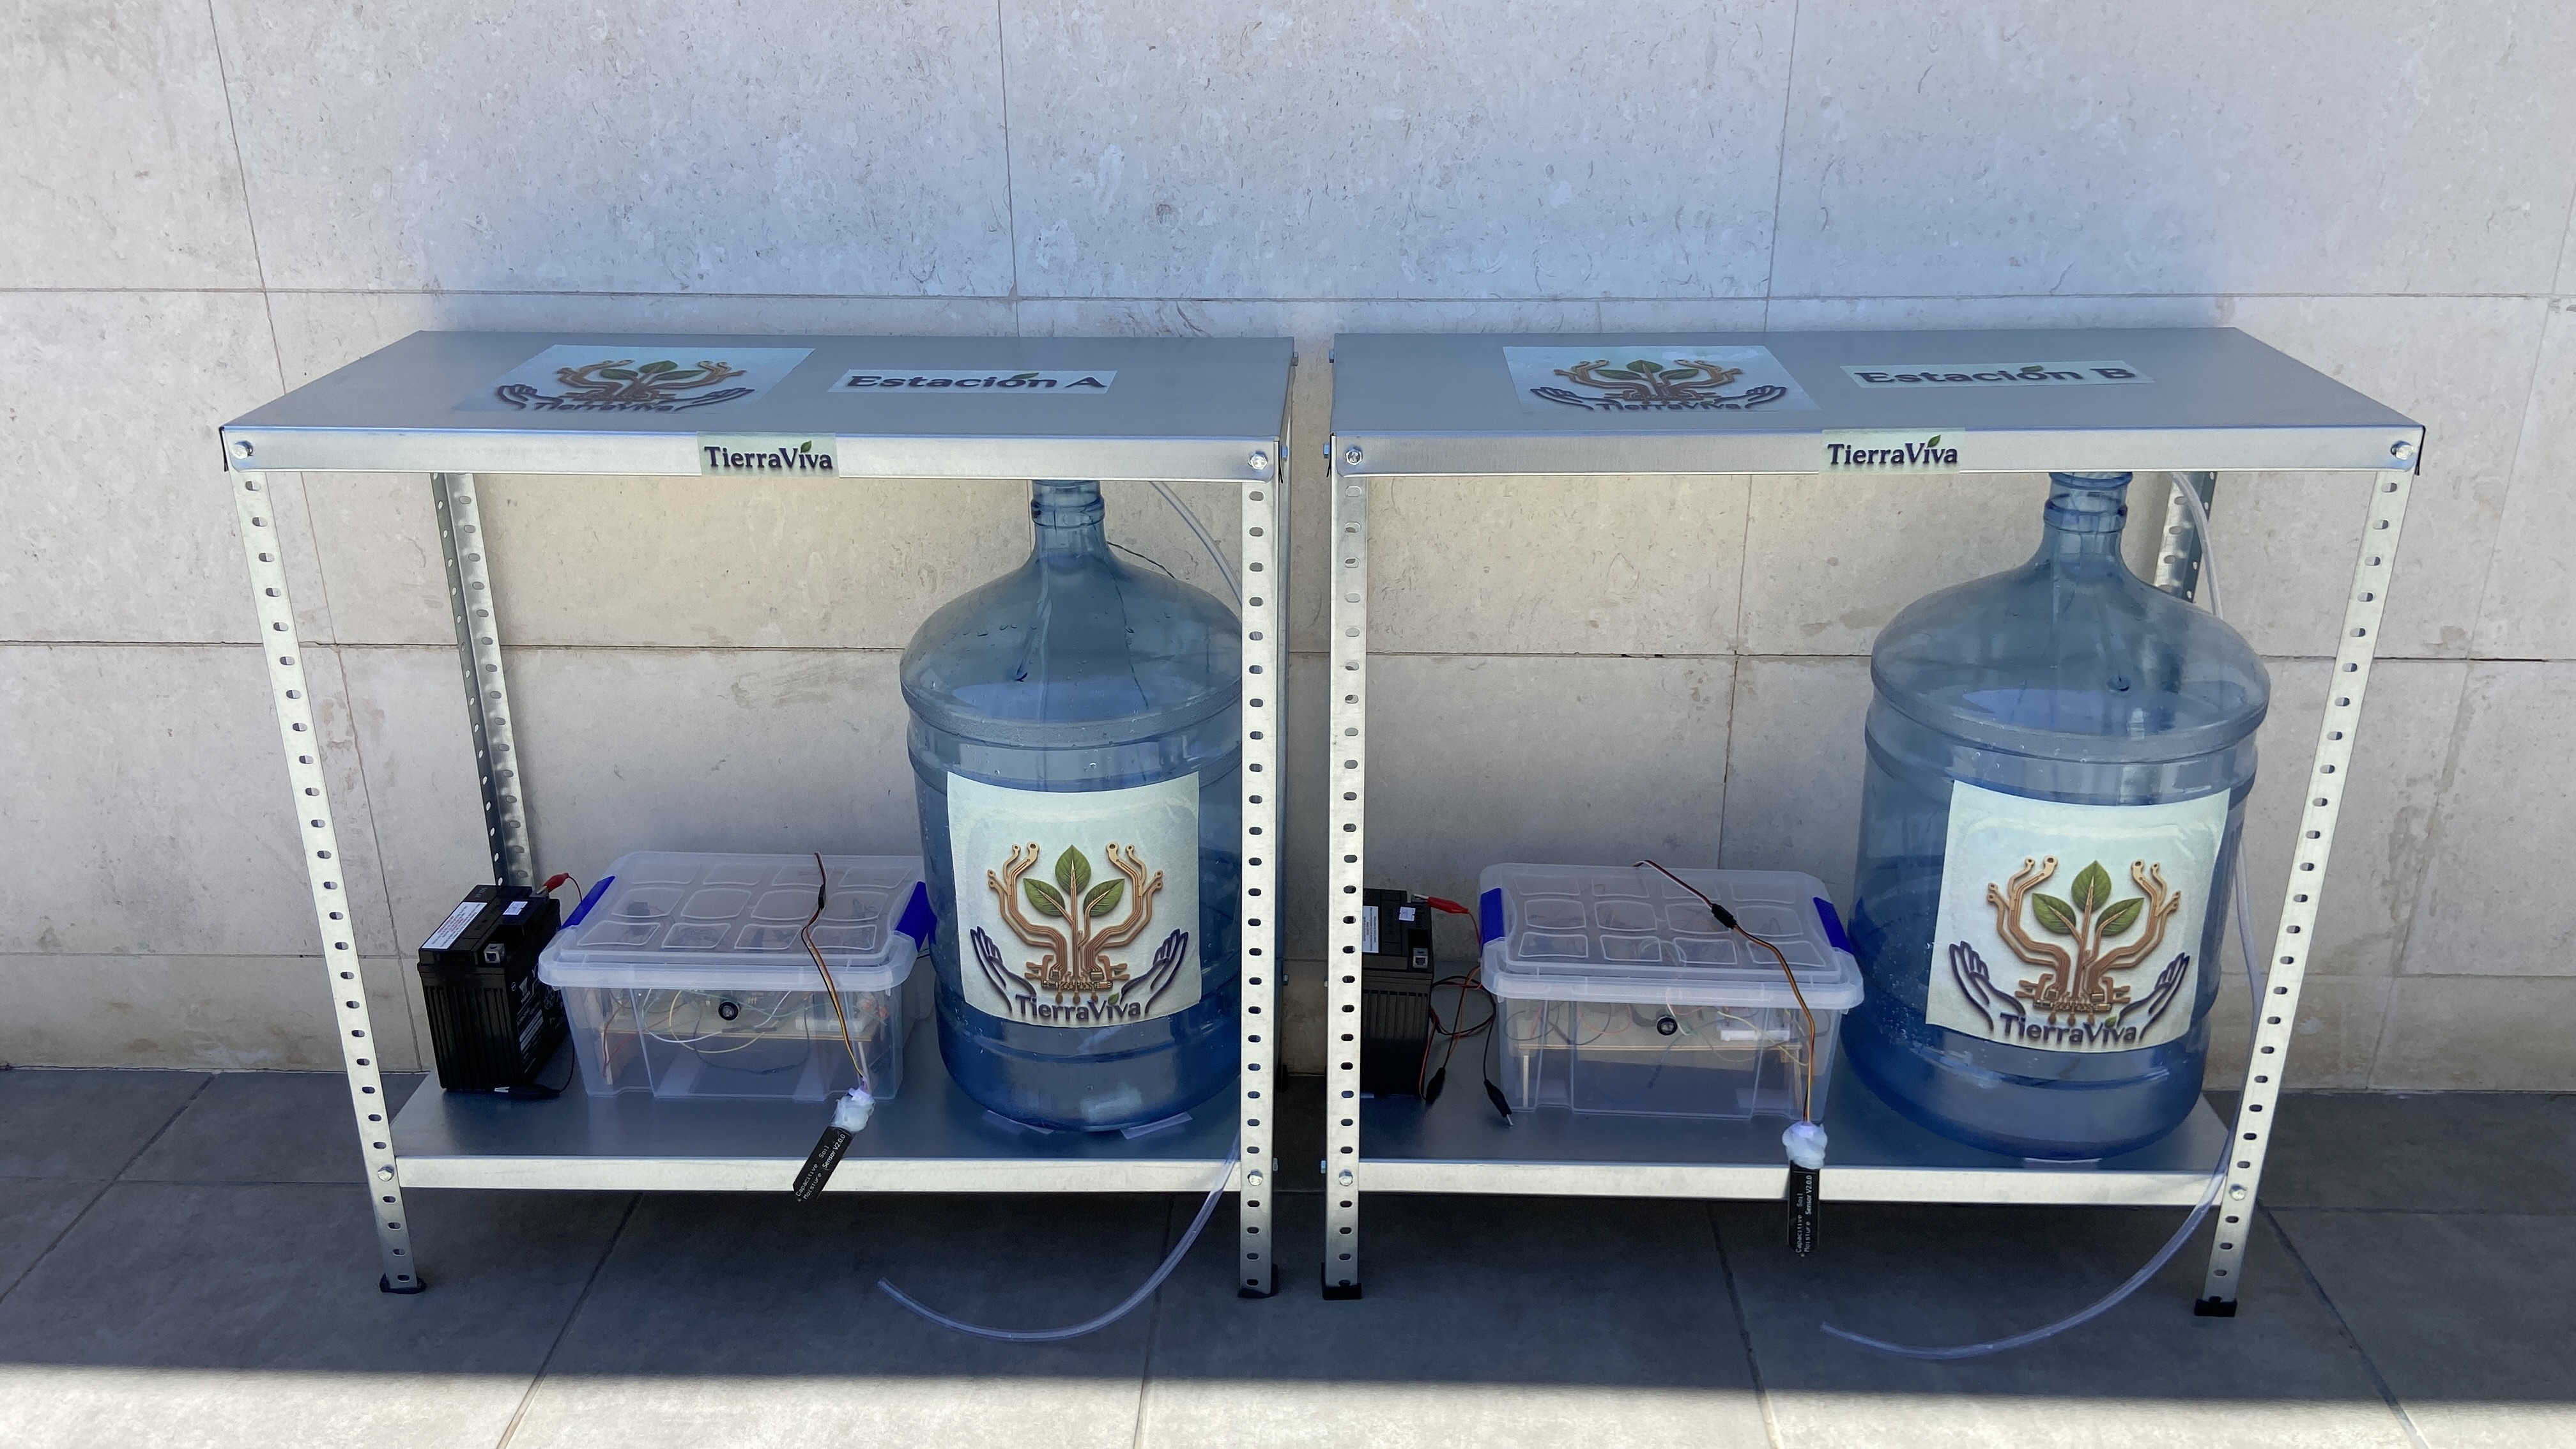
\includegraphics[width=0.82\textwidth]{figs/foto_estacion_validacion.jpg}
    \caption{Montaje físico utilizado para la validación de la estación remota (!!!!!cambiar por la definitiva!!!!!). Elaboración propia.}
    \label{fig:foto_estacion_validacion}
\end{figure}

La primera comprobación fue la programación del Arduino UNO compatible. Tras instalar el controlador del conversor \texttt{CH340G}, la placa fue reconocida en Windows como puerto \texttt{COM3} y se validó la carga del ejemplo \textit{Blink}. Con ello quedó comprobada la cadena básica de programación: detección USB, selección de placa, compilación, carga y ejecución.

Después se validó el bloque de sensórica. El escaneo I2C detectó el BH1750 en \texttt{0x23} y el BME280 en \texttt{0x76}, confirmando que ambos sensores podían compartir las líneas \texttt{A4/SDA} y \texttt{A5/SCL}. El sensor capacitivo de humedad de suelo se comprobó mediante lectura analógica en \texttt{A0}, observándose variaciones claras al modificar las condiciones de contacto del sensor.

Finalmente, se ejecutó el \textit{firmware} conjunto de estación. Esta prueba confirmó que el Arduino podía leer humedad de suelo, temperatura, humedad relativa, presión y luminosidad en un mismo ciclo, actualizar su estado interno y dejar preparada una muestra completa de telemetría para su publicación.

La actuación se validó de forma progresiva: primero mediante relé e indicador visual, y después con la bomba de agua de 12 V como carga real. La prueba confirmó que el \textit{firmware} activa el relé durante un intervalo limitado y lo apaga explícitamente al finalizar.

\section{Validación de comunicación, ThingSpeak y supervisión}
\label{sec:validacion_comunicacion_supervision}

La comunicación remota se validó primero de forma independiente y después integrada con Arduino. El A7670E-LASA respondió correctamente a comandos AT desde ordenador, reconoció la SIM, obtuvo señal, registró red LTE y permitió ejecutar peticiones HTTP. Posteriormente, el módem se conectó al Arduino mediante \texttt{SoftwareSerial}, trabajando a \texttt{9600} baudios para priorizar estabilidad.

La publicación en ThingSpeak se consideró válida cuando la estación obtuvo una respuesta HTTP correcta y los datos aparecieron en el canal correspondiente. Cada envío incluye humedad de suelo, temperatura, humedad relativa, luminosidad, presión, estado del relé, evento de sistema y código auxiliar de diagnóstico. La estructura completa de campos y códigos se documenta en el Anexo~\ref{anexo:estructura_thingspeak_estados}.

La Raspberry Pi se validó consultando los canales ThingSpeak, evitando duplicados mediante \texttt{entry\_id}, registrando lecturas en SQLite y exponiendo los datos mediante FastAPI. El \textit{dashboard} confirmó la visualización final de las lecturas, el estado de conexión, la antigüedad del dato, gráficas históricas y selección de estación.

La Figura~\ref{fig:evidencias_validacion_tierraviva} recoge cuatro evidencias visuales del flujo completo de validación: publicación en ThingSpeak, visualización en el \textit{dashboard}, inicialización de la estación desde monitor serie y ciclos de decisión local de riego. Esta composición permite conservar evidencia experimental real sin duplicar figuras extensas en el cuerpo principal de la memoria.

\begin{figure}[H]
\centering

\begin{minipage}{0.48\textwidth}
    \centering
    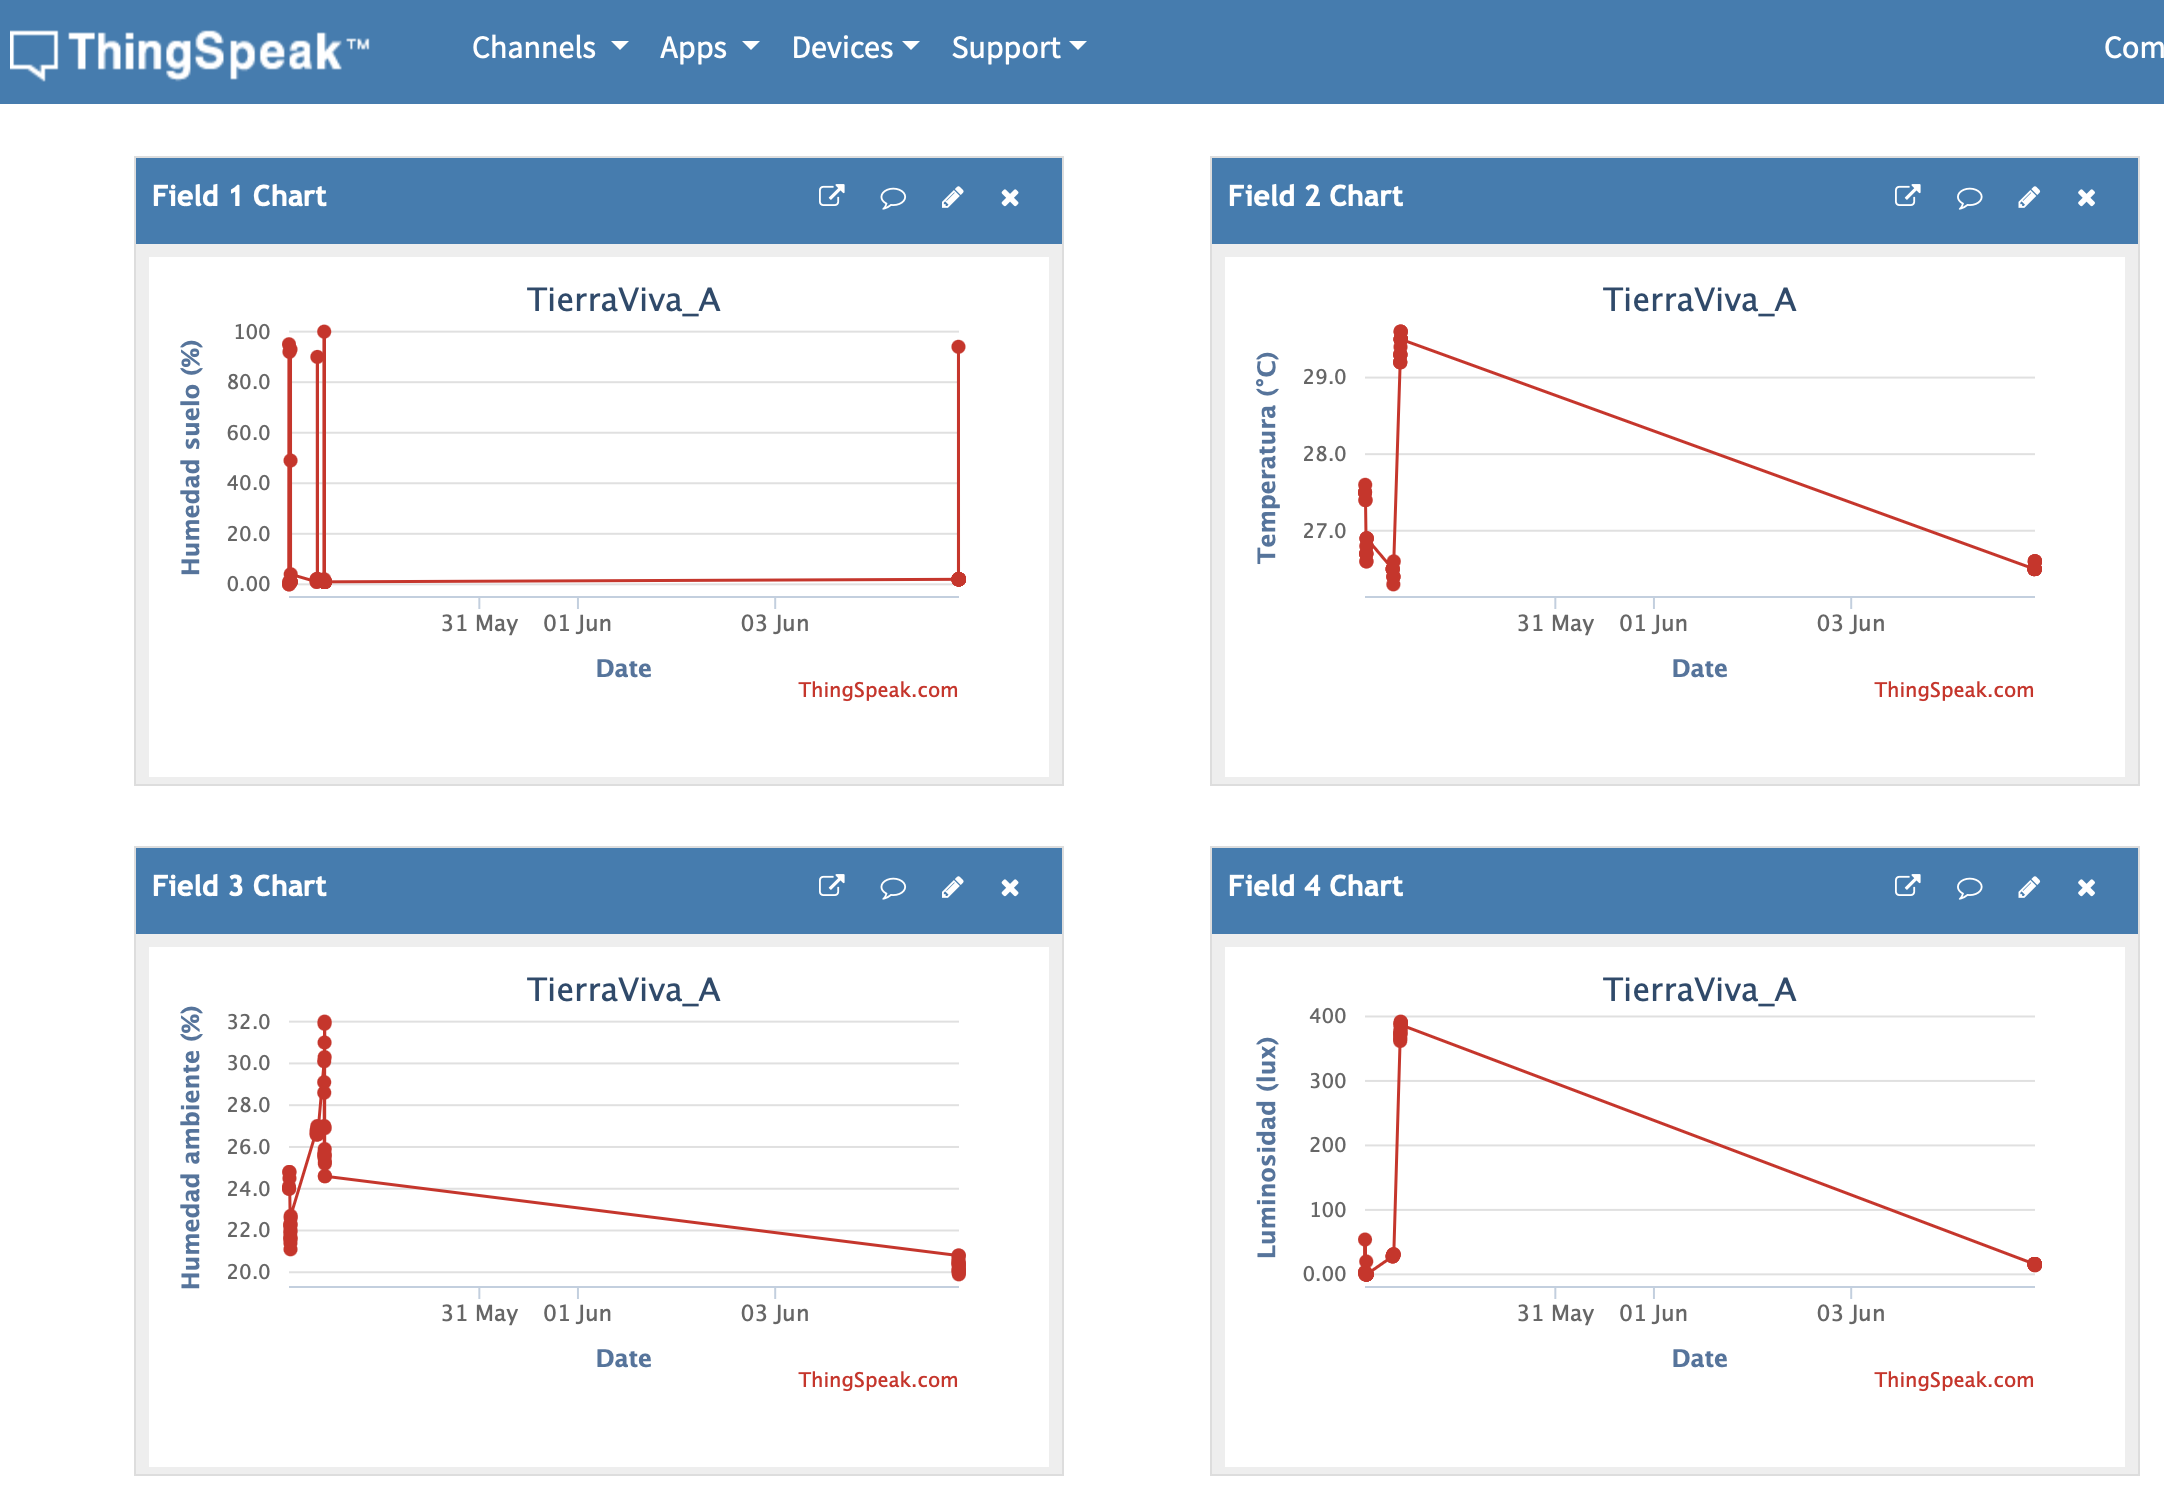
\includegraphics[width=\textwidth]{figs_png/evidencia_thingspeak_publicacion.png}
    \small (a) Publicación de telemetría en ThingSpeak.
\end{minipage}
\hfill
\begin{minipage}{0.48\textwidth}
    \centering
    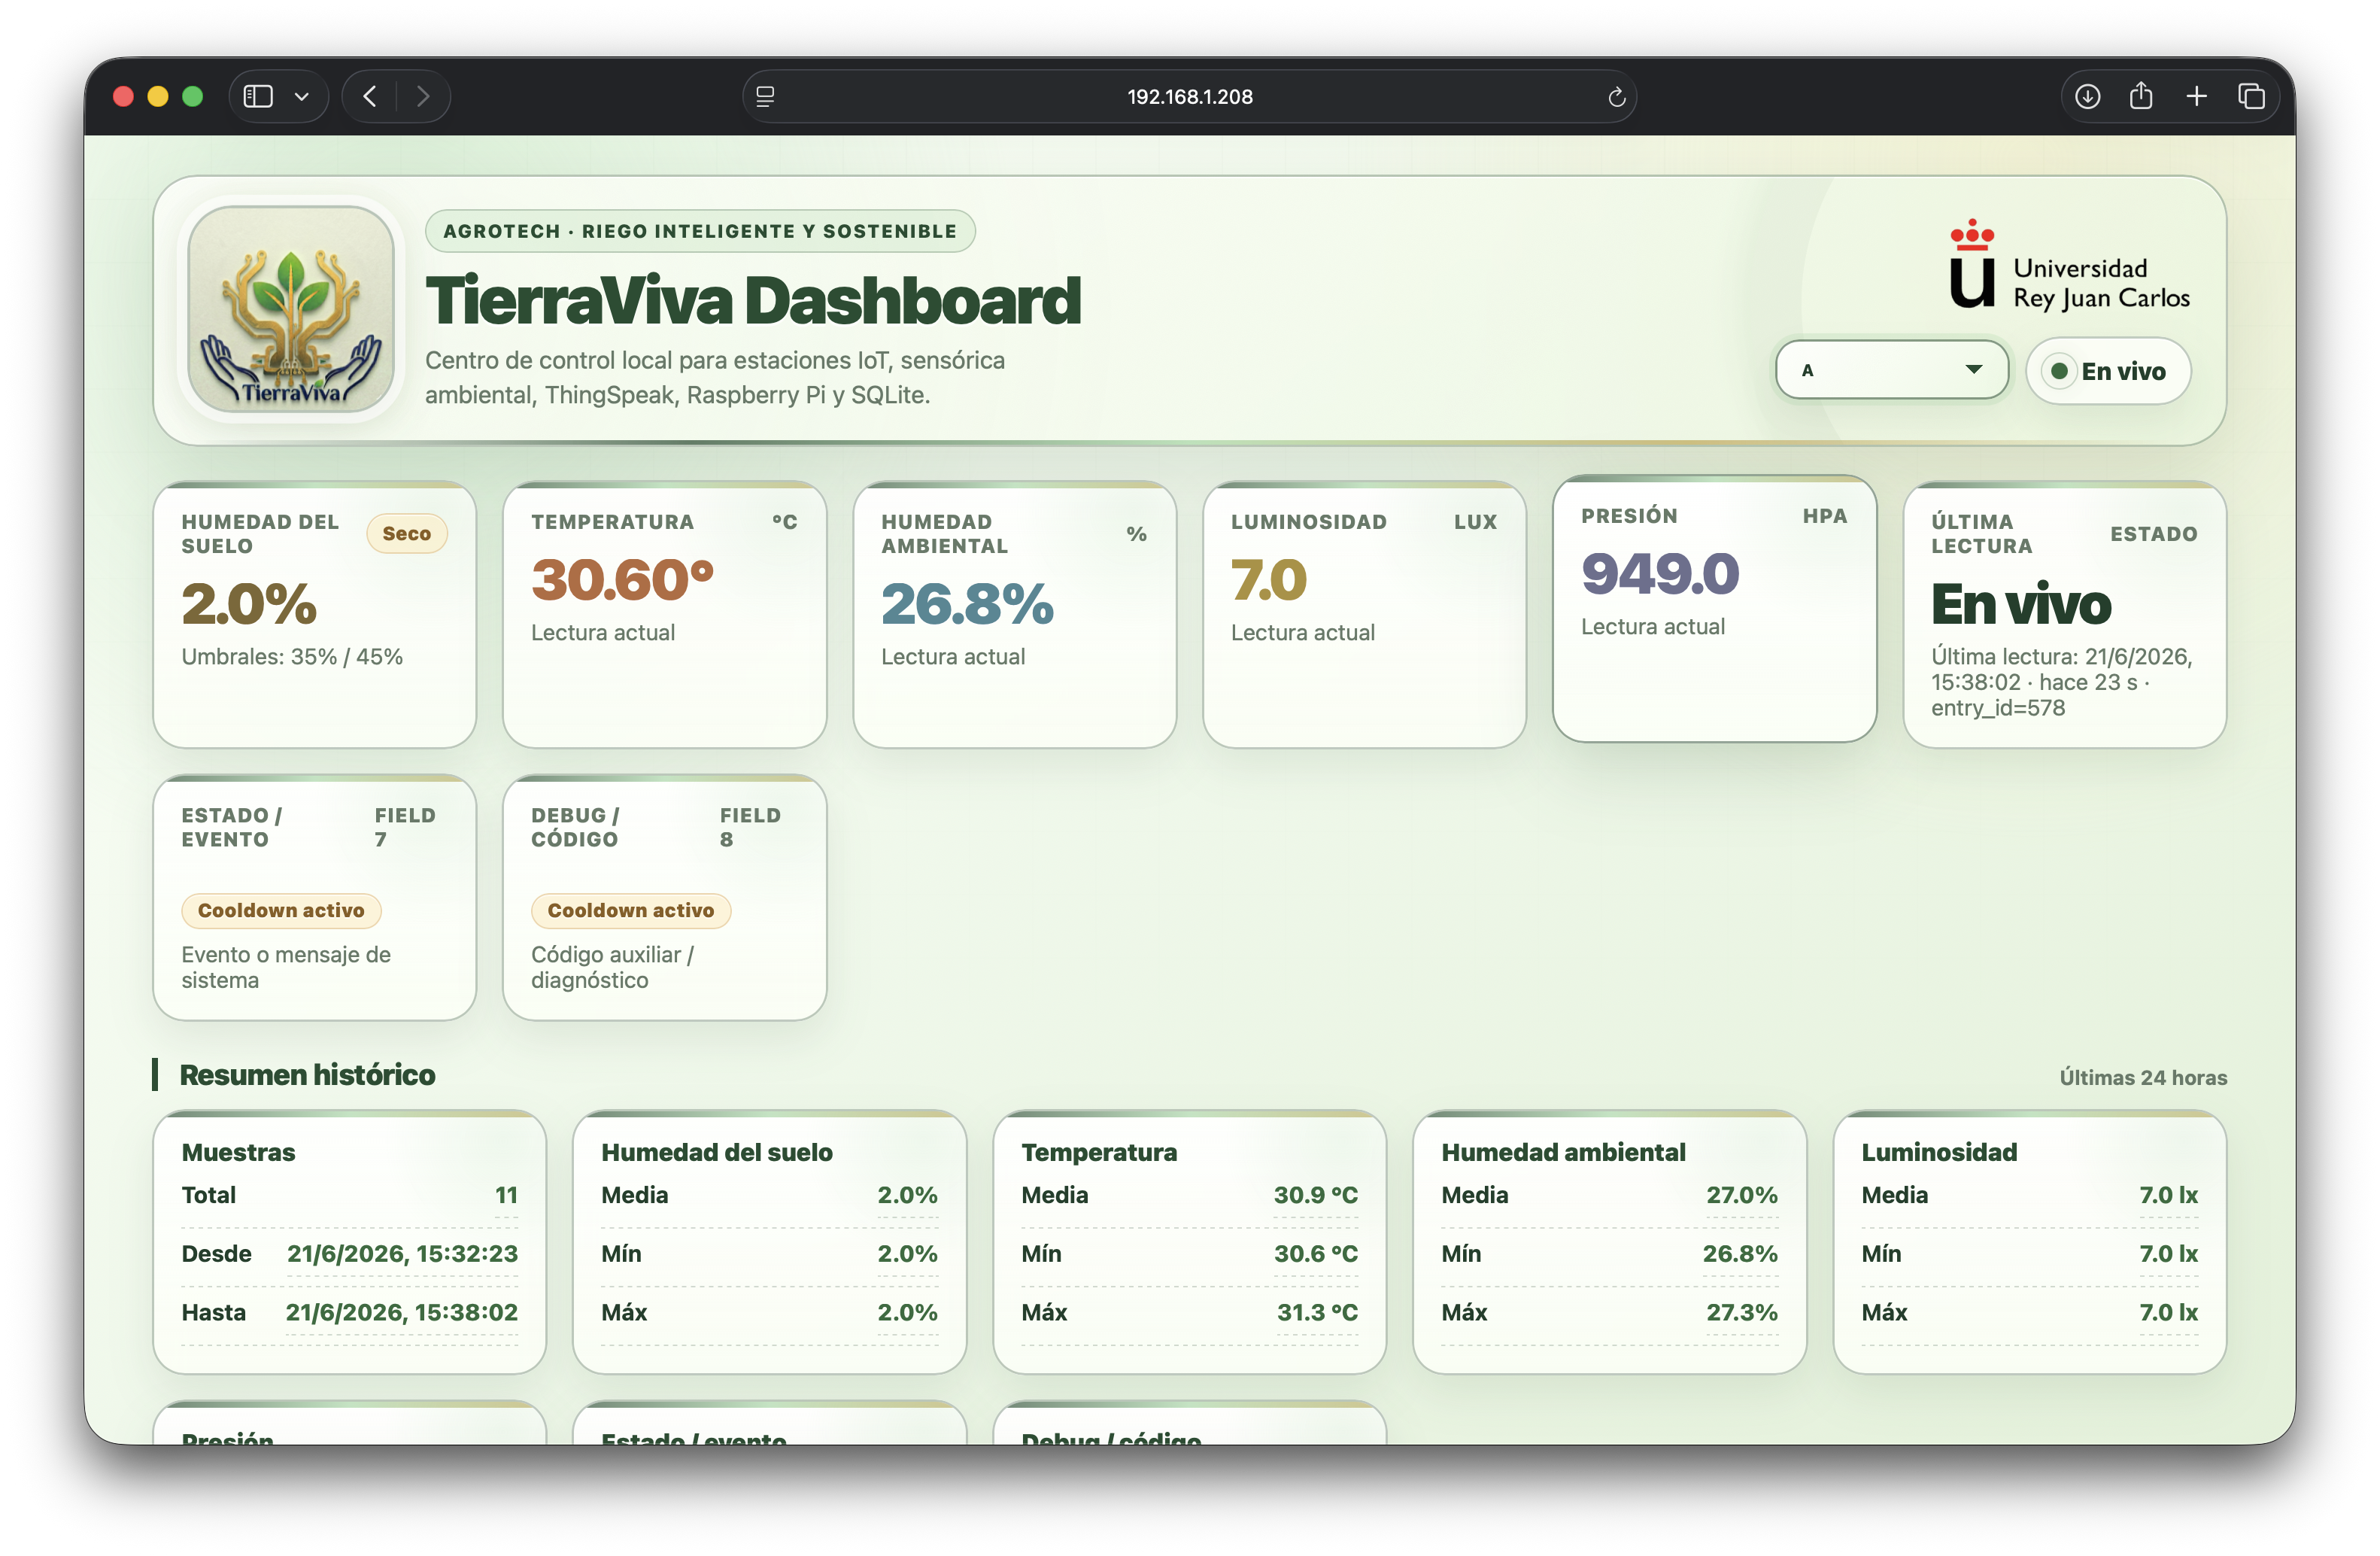
\includegraphics[width=\textwidth]{figs_png/evidencia_dashboard.png}
    \small (b) Visualización en el \textit{dashboard} local.
\end{minipage}

\vspace{0.35cm}

\begin{minipage}{0.48\textwidth}
    \centering
    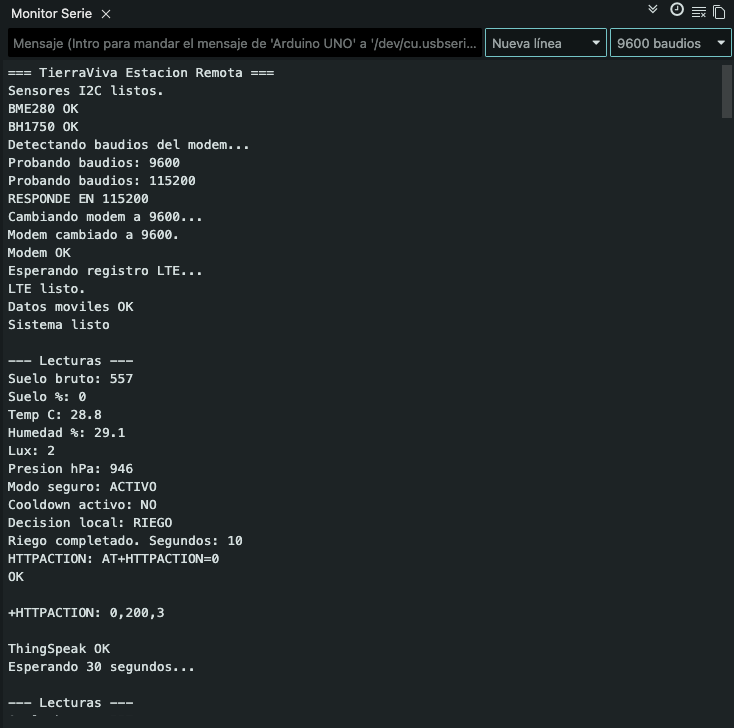
\includegraphics[width=\textwidth]{figs_png/monitor_serie_inicio_lte_thingspeak.png}
    \small (c) Inicialización, registro LTE y publicación HTTP correcta.
\end{minipage}
\hfill
\begin{minipage}{0.48\textwidth}
    \centering
    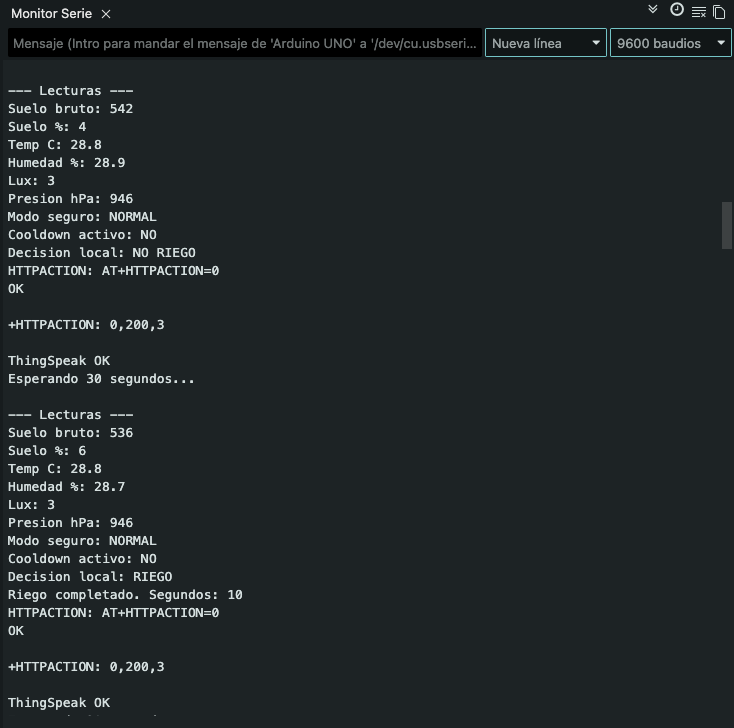
\includegraphics[width=\textwidth]{figs_png/monitor_serie_decision_riego_cooldown.png}
    \small (d) Ciclos de decisión local, riego y \textit{cooldown}.
\end{minipage}

\caption[Evidencias visuales del flujo completo de validación]{Evidencias visuales del flujo completo de validación de TierraViva. Se documenta la publicación de telemetría en ThingSpeak, la visualización desde el \textit{dashboard}, la inicialización de la estación mediante monitor serie y la ejecución de ciclos de decisión local con riego temporizado y bloqueo por \textit{cooldown}. Capturas propias.}
\label{fig:evidencias_validacion_tierraviva}
\end{figure}

Los registros completos asociados a estas capturas se recogen en el Anexo~\ref{subsec:evidencias_monitor_serie_pruebas}.

\section{Prueba funcional en entorno real en Agrolab Móstoles}
\label{sec:validacion_agrolab_mostoles}

Como cierre de la validación, se realizó una prueba funcional en Agrolab Móstoles, un entorno de agricultura urbana/periurbana situado en Móstoles, Madrid. Esta prueba se plantea como una comprobación funcional del prototipo fuera del entorno de laboratorio, orientada a verificar el comportamiento del sistema en una zona de cultivo real.

Durante la prueba se verificó el funcionamiento integrado de la estación de campo, la lectura de sensores, la comunicación LTE, la publicación de telemetría en ThingSpeak, la supervisión desde Raspberry Pi, la visualización en el \textit{dashboard} y la actuación controlada del riego. La prueba permitió comprobar que el sistema mantiene el mismo flujo funcional en un entorno real de cultivo: medir, decidir localmente, actuar de forma temporizada, publicar estado y permitir la supervisión posterior.

\begin{figure}[H]
    \centering
    %
\includegraphics[width=0.82\textwidth]{figs_png/prueba_agrolab_mostoles.png}
    \caption[Prueba funcional de TierraViva en Agrolab Móstoles]{Prueba funcional de TierraViva en Agrolab Móstoles. Vídeo de la prueba disponible en: \url{https://github.com/ltejedorcruz/TierraViva/ENLACE-PENDIENTE-VIDEO-AGROLAB}}
    \label{fig:prueba_agrolab_mostoles}
\end{figure}

La evidencia principal de esta prueba queda formada por la fotografía del montaje en Agrolab, las capturas de ThingSpeak y \textit{dashboard}, y el vídeo de funcionamiento. Por su alcance temporal, la prueba se documenta como validación funcional en entorno real, reservando las campañas agronómicas completas y los ensayos estacionales prolongados para futuras fases del proyecto.

\section{Validación de actuación y seguridad funcional}
\label{sec:validacion_actuacion_seguridad}

La validación de la actuación se trató como una parte crítica del proyecto, ya que TierraViva acciona físicamente una bomba de agua. La comprobación debía cubrir tanto la activación correcta del relé como el mantenimiento de la bomba apagada ante condiciones no fiables.

Las pruebas se centraron en seis situaciones: arranque de estación, riego autorizado, \textit{cooldown} activo, lectura inválida, pérdida temporal de comunicación y fallo de supervisión en Raspberry Pi. En todos los casos se verificó que la estación mantenía la lógica crítica de actuación y ejecutaba el apagado de la bomba mediante temporización local de \textit{firmware}.

El detalle de las ejecuciones registradas en el monitor serie se recoge en el Anexo~\ref{subsec:evidencias_monitor_serie_pruebas}, donde se muestran ciclos representativos con \texttt{NO RIEGO}, \texttt{RIEGO}, bloqueo por \textit{cooldown}, actuación temporizada de 10 segundos y publicación correcta en ThingSpeak.

La Tabla~\ref{tab:cap7_seguridad_funcional} resume las pruebas de seguridad funcional más relevantes.

\begin{table}[H]
\centering
\small
\renewcommand{\arraystretch}{1.15}
\rowcolors{2}{TableRowSoft}{white}
\begin{tabular}{|p{0.30\textwidth}|p{0.38\textwidth}|p{0.22\textwidth}|}
\hline
\rowcolor{URJCRed}
\TVHead{Condición validada} & \TVHead{Comportamiento observado} & \TVHead{Resultado} \\
\hline
Arranque de estación & El relé comienza apagado y la bomba permanece desactivada. & Correcto \\
\hline
Riego autorizado & La bomba se activa durante el tiempo configurado y se apaga al finalizar. & Correcto \\
\hline
\textit{Cooldown} activo & La estación bloquea una nueva actuación antes del tiempo mínimo. & Correcto \\
\hline
Lectura inválida & El \textit{firmware} mantiene la bomba apagada y publica estado de error. & Correcto \\
\hline
Pérdida temporal de comunicación & La estación mantiene control local y conserva un comportamiento seguro. & Correcto \\
\hline
Fallo de supervisión Raspberry & La estación conserva su lógica local de seguridad. & Correcto \\
\hline
\end{tabular}
\caption{Validación de seguridad funcional sobre la actuación de riego.}
\label{tab:cap7_seguridad_funcional}
\end{table}

Estas pruebas demuestran que el prototipo incorpora una lógica de actuación prudente. La decisión de riego se ejecuta localmente en la estación, con una actuación limitada en el tiempo y protegida por \textit{cooldown}, validación de sensores y estado seguro por defecto. El análisis completo de riesgos asociados se recoge en el Anexo~\ref{anexo:gestion_riesgos}.

\section{Conclusión de la validación}
\label{sec:conclusion_validacion}

La validación realizada permite afirmar que TierraViva cumple el objetivo de integrar una estación IoT autónoma con sensórica ambiental, comunicación LTE, publicación en ThingSpeak, supervisión en Raspberry Pi, almacenamiento local, API, \textit{dashboard} y actuación sobre riego. El sistema ha sido probado desde componentes individuales hasta el flujo completo extremo a extremo.

Las pruebas confirman la lectura conjunta de humedad del suelo, temperatura, humedad relativa, presión y luminosidad; el uso del A7670E-LASA mediante comandos AT, registro LTE y publicación HTTP; la consulta desde Raspberry Pi; el almacenamiento en SQLite; la exposición mediante API; la visualización en \textit{dashboard}; la actuación local sobre relé y bomba con temporización, \textit{cooldown} y apagado seguro; y la prueba funcional del prototipo en Agrolab Móstoles como entorno real de cultivo.

La validación también permite identificar las limitaciones de esta versión: calibración agronómica todavía limitada del sensor de humedad de suelo, dependencia de cobertura LTE, consumo del módulo A7670E-LASA, uso de ThingSpeak como plataforma de supervisión no estrictamente en tiempo real y necesidad de ensayos prolongados en campo.

En conjunto, el resultado de la validación es satisfactorio para el alcance del Trabajo de Fin de Grado. El prototipo se presenta como una arquitectura funcional, modular y verificable que demuestra el ciclo completo de monitorización y riego inteligente.


\chapter{Resultados, discusión y proyección del sistema}
\label{cap:resultados_discusion_conclusiones}

Tras la implementación y validación de TierraViva, este capítulo sintetiza los resultados obtenidos y discute el alcance real del sistema desarrollado. La finalidad es valorar el prototipo como una solución completa: qué se ha conseguido, qué decisiones han sido más relevantes, cómo se ha comportado en pruebas reales y qué mejoras permitirían evolucionarlo hacia una versión más robusta.

El resultado final de TierraViva es un sistema IoT funcional formado por dos estaciones remotas, comunicación LTE, publicación en ThingSpeak, supervisión local en Raspberry Pi, almacenamiento en SQLite, API FastAPI, \textit{dashboard} web y actuación física sobre riego. Esta integración es el aspecto central del trabajo: el sistema mide, decide, actúa, publica, almacena y visualiza.

\section{Resultados integrados del prototipo}
\label{sec:resultados_integrados}

El resultado principal del proyecto es la construcción y validación de un prototipo de riego inteligente basado en estaciones autónomas. Las estaciones A y B han sido montadas y probadas siguiendo una arquitectura equivalente, con sensórica ambiental y de suelo, módulo LTE A7670E-LASA, relé, bomba de agua y alimentación independiente.

Cada estación ejecuta localmente el \textit{firmware} de adquisición, decisión y actuación. La Raspberry Pi actúa como nodo de supervisión: consulta ThingSpeak, almacena lecturas en SQLite, expone datos mediante API y sirve el \textit{dashboard}. Esta separación permite que la actuación crítica permanezca en la estación incluso si la supervisión o la comunicación fallan temporalmente.

\begin{table}[H]
\centering
\scriptsize
\renewcommand{\arraystretch}{1.18}
\rowcolors{2}{TableRowSoft}{white}
\begin{tabular}{|p{0.24\textwidth}|p{0.40\textwidth}|p{0.26\textwidth}|}
\hline
\rowcolor{URJCRed}
\TVHead{Bloque} & \TVHead{Resultado conseguido} & \TVHead{Evidencia asociada} \\
\hline
Estaciones remotas & Dos estaciones físicas implementadas, configuradas. La estación B se empleó además en la prueba funcional en Agrolab Móstoles. & Montaje físico, vídeo, monitor serie y prueba funcional en entorno real. \\
\hline
Sensorización & Lectura conjunta de humedad del suelo, temperatura, humedad relativa, presión y luminosidad. & Escaneo I2C, lecturas analógicas, monitor serie y telemetría publicada. \\
\hline
Decisión local & Evaluación de humedad, modo seguro, confirmación de sequedad y bloqueo por \textit{cooldown}. & Código de decisión local y registros de monitor serie. \\
\hline
Actuación & Activación de bomba mediante relé, actuación temporizada y apagado explícito. & Pruebas P11--P13 y evidencia de riego temporizado. \\
\hline
Comunicación LTE & Publicación mediante A7670E-LASA, comandos AT y HTTP. & Respuesta \texttt{+HTTPACTION: 0,200,3} y datos visibles en ThingSpeak. \\
\hline
Telemetría & Publicación estructurada en \texttt{field1}--\texttt{field8} con variables físicas y estados internos. & Canales ThingSpeak y anexo de estructura de estados. \\
\hline
Supervisión local & Ingesta desde ThingSpeak, almacenamiento SQLite, API FastAPI y \textit{dashboard} web. & Base de datos local, endpoints API y visualización en navegador. \\
\hline
Validación real & Prueba funcional de una estación en Agrolab Móstoles, en zonas con diferente humedad de suelo. & Fotografías, vídeo, capturas, monitor serie y observación directa. \\
\hline
\end{tabular}
\caption{Resultados integrados obtenidos en el prototipo TierraViva.}
\label{tab:resultados_integrados_tierraviva}
\end{table}

El sistema validado cubre el flujo extremo a extremo planteado para el TFG: captación de datos, decisión local, actuación controlada, publicación remota, almacenamiento histórico, consulta mediante API y visualización en \textit{dashboard}.

\section{Cumplimiento de objetivos, requisitos y pruebas}
\label{sec:cumplimiento_objetivos_requisitos}

El grado de cumplimiento del proyecto debe valorarse comparando los resultados con los objetivos y requisitos definidos durante el diseño. Por ello, en esta sección no se evalúa únicamente si el prototipo “funciona”, sino si cubre las funciones, restricciones y criterios operativos establecidos en el Capítulo~\ref{cap:capitulo3} y trazados posteriormente en el Anexo~\ref{anexo:trazabilidad_requisitos_pruebas}.

\begingroup
\scriptsize
\renewcommand{\arraystretch}{1.18}
\rowcolors{2}{TableRowSoft}{white}

\begin{longtable}{|
>{\raggedright\arraybackslash}p{0.19\textwidth}|
>{\raggedright\arraybackslash}p{0.32\textwidth}|
>{\raggedright\arraybackslash}p{0.26\textwidth}|
>{\raggedright\arraybackslash}p{0.13\textwidth}|}

\caption{Cumplimiento de objetivos y requisitos a partir de las pruebas realizadas.}
\label{tab:cumplimiento_objetivos_requisitos}\\

\hline
\rowcolor{URJCRed}
\TVHead{Elemento evaluado} & \TVHead{Resultado observado} & \TVHead{Relación con requisitos/pruebas} & \TVHead{Estado} \\
\hline
\endfirsthead

\hline
\rowcolor{URJCRed}
\TVHead{Elemento evaluado} & \TVHead{Resultado observado} & \TVHead{Relación con requisitos/pruebas} & \TVHead{Estado} \\
\hline
\endhead

\hline
\multicolumn{4}{r}{\small Continúa en la página siguiente} \\
\endfoot

\hline
\endlastfoot

Medición de variables & La estación mide humedad de suelo, temperatura, humedad relativa, presión y luminosidad. & RF-01, RF-02, RF-03; P02--P04, P16. & Cumplido \\
\hline
Comunicación remota & La estación publica telemetría mediante LTE/HTTP en ThingSpeak. & RF-04, RF-10; P05, P06, P16. & Cumplido \\
\hline
Identificación multiestación & Las estaciones A y B se gestionan mediante canales e identificadores diferenciados. & RF-05, RNF-07; P07, P08, P10, P16. & Cumplido \\
\hline
Almacenamiento histórico & La Raspberry Pi conserva lecturas en SQLite evitando duplicados por \texttt{entry\_id}. & RF-06; P07, P08, P16. & Cumplido \\
\hline
Visualización & El \textit{dashboard} muestra lecturas, estado, histórico, gráficas y selección de estación. & RF-07, RNF-08; P09, P10, P16. & Cumplido \\
\hline
Decisión local de riego & El riego se decide en el \textit{firmware} de cada estación, a partir de las lecturas y reglas locales configuradas. & RF-08, RF-11, RNF-06; P13--P15. & Cumplido \\
\hline
Actuación segura & La bomba se activa por relé durante un tiempo limitado y se apaga explícitamente. & RF-09, ET-05, ET-08; P11, P12, P17. & Cumplido \\
\hline
Validación en entorno real & El prototipo se prueba en Agrolab Móstoles con la estación B, en un entorno real de cultivo y diferentes condiciones de humedad. & P17; validación funcional en entorno real. & Cumplido \\
\hline

\end{longtable}

\normalsize
\endgroup

Esta tabla permite cerrar el recorrido completo del proyecto: los requisitos no quedan como una lista teórica de diseño, sino vinculados a bloques implementados y pruebas realizadas.

\section{Discusión técnica de la arquitectura final}
\label{sec:discusion_tecnica_arquitectura}

La arquitectura final de TierraViva es el resultado de varias decisiones tomadas durante el desarrollo. La más importante ha sido mantener la actuación crítica en la estación. Ese reparto condiciona todo el sistema: la estación mide y decide localmente, mientras que ThingSpeak, la Raspberry Pi y el \textit{dashboard} se orientan a telemetría, almacenamiento, consulta y visualización.

En un sistema que actúa sobre agua, esta separación es especialmente importante. Si la decisión dependiera de la nube o de una conexión continua, una caída de red, una latencia elevada o una orden incorrecta podrían provocar un comportamiento no deseado. En TierraViva, una pérdida temporal de ThingSpeak afecta a la publicación de datos, pero no deja la bomba sin control.

El uso de LTE mediante A7670E-LASA también ha sido una decisión relevante. Frente a una solución basada únicamente en WiFi, LTE permite que la estación funcione en zonas donde no existe infraestructura local de red. A cambio, introduce más complejidad: comandos AT, alimentación más exigente, consumo superior, necesidad de SIM, cobertura y gestión de errores. El prototipo ha permitido comprobar que esta complejidad es asumible dentro del alcance del TFG, siempre que se valide de forma incremental.

ThingSpeak ha funcionado como una capa intermedia útil para telemetría. Su valor principal ha sido desacoplar las estaciones de la Raspberry Pi: la estación publica desde campo y la Raspberry consulta posteriormente. Su papel en TierraViva es recibir datos, conservarlos temporalmente y permitir su consulta como \textit{broker} de telemetría.

La Raspberry Pi aporta la parte de supervisión local. Al almacenar en SQLite, exponer una API y servir un \textit{dashboard}, el sistema gana trazabilidad, consulta histórica y una interfaz más adaptada al proyecto. Esta capa convierte una publicación aislada de sensores en un sistema supervisable.

La existencia de dos estaciones montadas y probadas refuerza la validez de la arquitectura. El modelo demuestra capacidad multiestación mediante identificadores y canales diferenciados, lo que permite escalar conceptualmente a más nodos manteniendo una lógica común de supervisión.

\section{Validación en Agrolab Móstoles y recepción cualitativa}
\label{sec:validacion_recepcion_agrolab}

La prueba funcional en Agrolab Móstoles tiene un valor especial dentro del proyecto porque traslada el prototipo fuera del entorno controlado de laboratorio. Agrolab Móstoles se enmarca en un Laboratorio de Agricultura Abierta impulsado por IMIDRA en colaboración con el Ayuntamiento de Móstoles, orientado a formación agraria, emprendimiento, agricultura social y prácticas de cultivo en un entorno real.

Durante la prueba final se desplegó la estación B en una zona de cultivo y se verificó el funcionamiento integrado del sistema: lectura de sensores, decisión local de riego, actuación temporizada de la bomba, publicación de telemetría en ThingSpeak, consulta desde Raspberry Pi y visualización en el \textit{dashboard}. La prueba no constituye una campaña agronómica prolongada, pero sí una validación funcional relevante en un contexto de uso real.

Además de la comprobación técnica, la prueba permitió recoger impresiones cualitativas de personas usuarias del espacio. Estas observaciones se incorporan como una primera recepción práctica del prototipo por parte de personas familiarizadas con el riego y el cuidado de cultivos.

\begin{table}[H]
\centering
\scriptsize
\renewcommand{\arraystretch}{1.18}
\rowcolors{2}{TableRowSoft}{white}
\begin{tabular}{|p{0.36\textwidth}|p{0.50\textwidth}|}
\hline
\rowcolor{URJCRed}
\TVHead{Comentario u observación recibida} & \TVHead{Interpretación para TierraViva} \\
\hline
Varios usuarios preguntaron dónde se había comprado el sistema. & El prototipo fue percibido como un sistema funcional y reconocible, no únicamente como un montaje experimental. \\
\hline
Al conocer que el sistema había sido construido desde cero, el interés aumentó. & Refuerza el valor del trabajo de integración: electrónica, \textit{firmware}, comunicación, plataforma y actuación fueron desarrollados y ajustados durante el TFG. \\
\hline
Una usuaria comentó que le resultaría útil cuando se ausenta y necesita que alguien riegue por ella. & Confirma una necesidad práctica real: automatizar el riego en ausencias y reducir la dependencia de terceras personas. \\
\hline
Algunas personas preguntaron si podría montarse o adaptarse para sus casas o huertos. & Indica interés de uso más allá de la demostración académica, aunque el prototipo no se presente como producto comercial final. \\
\hline
Se valoró positivamente que el sistema pudiera adaptarse con batería, panel solar, depósito mayor o distinta configuración. & Refuerza la importancia de la modularidad como decisión de diseño y como línea futura. \\
\hline
Se sugirió que el sistema tenía potencial suficiente como para protegerse o desarrollarse más. & Aunque se trata de un comentario informal, muestra una percepción positiva del valor práctico del prototipo. \\
\hline
\end{tabular}
\caption{Recepción cualitativa observada durante la prueba funcional en Agrolab Móstoles.}
\label{tab:recepcion_cualitativa_agrolab}
\end{table}

Para conservar el carácter real de la prueba sin introducir un tono coloquial excesivo en la memoria, los comentarios se han incorporado de forma anonimizada y resumida. El elemento común en la recepción recibida fue claro: el interés no se centró solo en la tecnología, sino en la utilidad práctica. Los usuarios valoraron especialmente que el sistema pudiera regar cuando la persona no está presente, que se pudiera consultar su estado y que fuera adaptable a depósitos, alimentación o necesidades distintas.

Esta recepción cualitativa refuerza una conclusión importante: TierraViva conecta la integración técnica IoT con una necesidad comprensible para usuarios reales de huertos urbanos y pequeñas zonas de cultivo. Esa relación entre implementación técnica y utilidad percibida es uno de los resultados más relevantes de la prueba en Agrolab.

\section{Limitaciones detectadas}
\label{sec:limitaciones_detectadas}

El prototipo ha cumplido los objetivos planteados, pero mantiene limitaciones que deben reconocerse para delimitar correctamente su alcance.

La primera limitación es la calibración agronómica del sensor de humedad del suelo. El sistema permite diferenciar situaciones secas y húmedas y activar el riego según umbrales, pero una calibración completa requeriría analizar distintos sustratos, profundidades, cultivos, tiempos de infiltración y evolución de humedad tras cada riego.

La segunda limitación es la dependencia de cobertura LTE y alimentación estable. El módulo A7670E-LASA permite independencia frente a WiFi local, pero requiere una alimentación robusta, una SIM operativa, cobertura suficiente y una gestión adecuada de errores. 

Otra limitación es la robustez física. El montaje actual permite validar la arquitectura y el funcionamiento, pero una versión de campo prolongada requeriría encapsulado, conectores adecuados, protección frente a humedad, organización del cableado y mayor resistencia mecánica.

Por último, la prueba en Agrolab Móstoles constituye una validación funcional en entorno real. Su alcance permite comprobar el comportamiento integrado del prototipo en una zona de cultivo, mientras que la cuantificación de ahorro hídrico, la mejora del rendimiento del cultivo y el comportamiento estacional requerirían campañas de larga duración y mediciones comparativas.

\section{Líneas futuras}
\label{sec:lineas_futuras}

Las líneas futuras de TierraViva se organizan en función de las limitaciones detectadas y de la recepción cualitativa obtenida durante la prueba en Agrolab.

Una primera evolución sería mejorar la calibración agronómica del sensor de humedad. Para ello sería necesario trabajar con distintos tipos de suelo, diferentes profundidades de sensor y mediciones repetidas tras ciclos de riego. Esta calibración permitiría ajustar los umbrales de forma menos experimental y más vinculada al comportamiento real del sustrato.

La segunda línea futura es la autonomía energética. La integración de panel solar, batería dimensionada y regulador de carga permitiría desplegar estaciones durante periodos más largos. Existen además iniciativas abiertas que exploran soluciones de riego alimentadas por energía solar en contextos comunitarios, como OSPIT \cite{apc2024,ospit2024}, por lo que esta línea encaja de forma natural con la evolución de TierraViva. Esta mejora fue especialmente coherente con los comentarios recibidos en Agrolab, donde se valoró la posibilidad de adaptar batería, alimentación y depósito a cada caso.

Una tercera línea es incorporar configuración remota desde el \textit{dashboard}. Esta mejora permitiría modificar umbrales de humedad, duración de riego, frecuencia de envío o parámetros de \textit{cooldown} sin reprogramar el Arduino. Su incorporación implicaría diseñar un canal descendente seguro, validación de órdenes, persistencia de configuración y límites que impidan actuaciones peligrosas.

También podría añadirse un modo de riego manual supervisado desde el \textit{dashboard}. Esta función permitiría activar un riego puntual bajo control del usuario, pero debería incorporar restricciones de seguridad: tiempo máximo, confirmación explícita, bloqueo por \textit{cooldown}, comprobación de estado de estación y registro del evento.

Otra línea relevante es la incorporación de inteligencia artificial o modelos predictivos. En una versión futura, con suficiente histórico de humedad, meteorología, riegos y respuesta del suelo, podrían entrenarse modelos para anticipar necesidades de riego o ajustar umbrales dinámicamente. Esta línea requiere un volumen de datos mayor y una campaña prolongada que permita validar predicciones de forma rigurosa.

También se podrían integrar sensores adicionales: caudalímetro para estimar volumen aplicado, sensor de nivel de depósito para evitar activar la bomba sin agua, pH, conductividad eléctrica o sensores meteorológicos complementarios. Estas variables permitirían pasar de un sistema de riego basado principalmente en humedad de suelo a una supervisión agronómica más completa.

Físicamente, una evolución natural sería diseñar una PCB propia, mejorar el encapsulado, emplear conectores estancos, ordenar el cableado y preparar una caja de campo. Estas mejoras no cambian la arquitectura conceptual, pero sí aumentarían la robustez y facilidad de instalación.

Finalmente, el sistema podría evolucionar hacia una gestión multiestación más avanzada. Esto incluiría alta y baja de estaciones desde el \textit{dashboard}, comparación entre zonas de cultivo, reglas por estación, agrupación por parcelas y alertas de funcionamiento anómalo.

\section{Alineación ambiental y social}
\label{sec:alineacion_ambiental_social}

La alineación de TierraViva con los Objetivos de Desarrollo Sostenible se entiende como una contribución potencial dentro del alcance de un prototipo académico. El sistema materializa una arquitectura orientada a medir condiciones reales del entorno, evitar actuaciones de riego puramente fijas, supervisar el estado del sistema y facilitar futuras optimizaciones basadas en datos. La cuantificación de ahorro hídrico y la demostración de mejoras agronómicas prolongadas quedan reservadas para fases posteriores de validación.

\begin{table}[H]
\centering
\scriptsize
\renewcommand{\arraystretch}{1.16}
\rowcolors{2}{TableRowSoft}{white}
\begin{tabular}{|p{0.13\textwidth}|p{0.32\textwidth}|p{0.43\textwidth}|}
\hline
\rowcolor{URJCRed}
\TVHead{ODS} & \TVHead{Relación con TierraViva} & \TVHead{Resultado o alcance real del prototipo} \\
\hline
ODS 2 & Agricultura más sostenible y apoyada en datos. & Las estaciones permiten observar humedad del suelo y variables ambientales para apoyar decisiones de riego más informadas. \\
\hline
ODS 6 & Uso más eficiente del agua. & El riego se activa por lógica local y durante un tiempo limitado, aunque no se cuantifica todavía ahorro hídrico. \\
\hline
ODS 12 & Uso responsable y adaptable de recursos. & El diseño modular permite adaptar batería, depósito, alimentación o número de estaciones según el escenario. \\
\hline
ODS 13 & Observación ambiental y adaptación futura. & El histórico de datos puede servir como base para analizar condiciones ambientales y mejorar reglas de riego en versiones posteriores. \\
\hline
\end{tabular}
\caption{Alineación de TierraViva con los Objetivos de Desarrollo Sostenible dentro del alcance del prototipo.}
\label{tab:alineacion_ods_tierraviva}
\end{table}

Desde el punto de vista social, la prueba en Agrolab Móstoles mostró que el sistema puede resultar comprensible y útil para usuarios no técnicos, especialmente por la posibilidad de supervisar el estado del riego, automatizar actuaciones durante ausencias y adaptar el montaje a distintas necesidades. Esta recepción refuerza el valor del prototipo tanto por su integración tecnológica como por su aplicabilidad en huertos urbanos y pequeñas zonas de cultivo.

\section{Conclusiones finales}
\label{sec:conclusiones_finales}

El Trabajo de Fin de Grado ha permitido diseñar, implementar y validar TierraViva, un prototipo IoT de riego inteligente formado por dos estaciones remotas, comunicación LTE, telemetría en ThingSpeak, supervisión en Raspberry Pi, almacenamiento SQLite, API FastAPI, \textit{dashboard} web y actuación física mediante relé y bomba de agua.

El sistema demuestra el ciclo completo de funcionamiento: mide variables del entorno y del suelo, interpreta la humedad mediante \textit{firmware}, decide localmente si debe regar, activa la bomba durante un tiempo limitado, publica su estado y permite supervisar los datos de forma local y remota. Esta integración confirma el desarrollo de una arquitectura funcional de extremo a extremo.

La decisión de mantener el control crítico en la estación ha sido esencial. Gracias a ella, la pérdida de comunicación con ThingSpeak, la caída del nodo de supervisión o la ausencia del \textit{dashboard} conservan la actuación bajo la lógica local del \textit{firmware}. Esta separación entre actuación local y supervisión remota es una de las aportaciones técnicas más importantes del proyecto.

La validación en Agrolab Móstoles aporta una dimensión adicional: el sistema no solo funcionó en entorno controlado, sino que fue probado en una zona real de cultivo y ante usuarios potenciales. La recepción cualitativa obtenida mostró interés por la utilidad del sistema, especialmente para ausencias, supervisión remota y adaptación modular.

TierraViva mantiene limitaciones: calibración agronómica todavía inicial, dependencia de cobertura LTE, consumo del módulo celular, ausencia de encapsulado definitivo y falta de campañas prolongadas. Sin embargo, estas limitaciones están identificadas y conducen a líneas futuras claras: energía solar, configuración remota, riego manual seguro, IA predictiva, sensores adicionales, encapsulado, PCB y gestión multiestación avanzada.

En conjunto, TierraViva cumple los objetivos del TFG y constituye una base técnica sólida, funcional, estable, modular y escalable. El resultado es un prototipo académico avanzado que demuestra la viabilidad de integrar sensórica, comunicaciones móviles, supervisión software y actuación local segura para riego inteligente.


\cleardoublepage
\phantomsection
\addcontentsline{toc}{chapter}{ANEXOS}
\chapter*{ANEXOS}
\markboth{ANEXOS}{ANEXOS}

\makeatletter
\def\@Alph#1{%
  \ifcase#1\or A\or B\or C\or D\or E\or F\or G\or H\or I\or J\or K\or L\or M\or N\or O\or P\or Q\or R\or S\or T\or U\or V\or W\or X\or Y\or Z\else\@ctrerr\fi}
\makeatother

\appendix

\chapter{Cronograma del proyecto}
\label{anexo:cronograma}

Este anexo recoge la planificación temporal seguida durante el desarrollo de TierraViva, desde el inicio del Trabajo de Fin de Grado a finales de agosto de 2025 hasta la entrega y defensa previstas en julio de 2026. El cronograma no se plantea como una secuencia rígida y lineal, sino como la reconstrucción ordenada del trabajo real realizado: definición inicial, revisión tecnológica, primeros prototipos, reajuste de arquitectura, implementación \textit{hardware} y \textit{software}, validación funcional, prueba en Agrolab Móstoles y redacción progresiva de la memoria.

TierraViva ha requerido integrar electrónica, \textit{firmware}, comunicaciones móviles, plataforma \textit{cloud}, base de datos, API, \textit{dashboard}, actuación física sobre bomba de agua y documentación técnica. Por ello, varias tareas se han desarrollado en paralelo y otras han requerido iteraciones, correcciones y cambios de enfoque.

\section{Periodo de desarrollo}

El desarrollo efectivo del proyecto se extiende desde finales de agosto de 2025 hasta julio de 2026. La entrega de la memoria se sitúa entre los días 6 y 11 de julio de 2026, y la defensa está prevista entre los días 21 y 24 de julio de 2026.

\small
\renewcommand{\arraystretch}{1.15}
\rowcolors{2}{TableRowSoft}{white}

\begin{longtable}{|p{0.22\textwidth}|p{0.64\textwidth}|}
\caption{Resumen temporal del desarrollo del proyecto TierraViva.}
\label{cuadro:resumen_temporal_cronograma}\\
\hline
\rowcolor{URJCRed}
\TVHead{Periodo} & \TVHead{Caracterización del trabajo realizado} \\
\hline
\endfirsthead

\hline
\rowcolor{URJCRed}
\TVHead{Periodo} & \TVHead{Caracterización del trabajo realizado} \\
\hline
\endhead

Finales de agosto--octubre de 2025 & Inicio del TFG, definición de la idea, planificación inicial, primera propuesta al tutor y revisión bibliográfica. Septiembre y octubre tuvieron una dedicación más orientada a análisis, búsqueda de información y organización del alcance. \\
\hline
Noviembre--diciembre de 2025 & Consolidación del estado del arte, definición inicial de requisitos y arquitectura, primeros enfoques de prototipado local y selección inicial de tecnologías. \\
\hline
Enero--febrero de 2026 & Trabajo con Arduino, sensores y primeros montajes. Reajuste progresivo desde un enfoque más local hacia una arquitectura con estaciones remotas, conectividad LTE y ThingSpeak. Enero tuvo menor disponibilidad por exámenes. \\
\hline
Marzo--abril de 2026 & Desarrollo intensivo de comunicaciones, backend, base de datos, API y soporte multiestación. En abril se realizó una visita previa a Agrolab Móstoles junto con Ana Zazo, co-tutora del proyecto. \\
\hline
Mayo de 2026 & Consolidación del \textit{firmware} de estación, decisión local de riego, \textit{cooldown}, publicación HTTP, redacción seria de la memoria y cierre de los primeros capítulos técnicos. Mayo tuvo menor disponibilidad por exámenes, compensada con jornadas intensivas fuera del periodo de evaluación. \\
\hline
Junio de 2026 & Montaje de la estación B, versión final del \textit{dashboard}, ajustes eléctricos, validación funcional, prueba en Agrolab Móstoles el 22 de junio, fotografías, vídeo, evidencias y cierre de capítulos finales y anexos. \\
\hline
Julio de 2026 & Revisión final de memoria, formato, trazabilidad, entrega y preparación de la defensa. \\
\hline
\end{longtable}

\normalsize

\section{Fases principales del proyecto}

La Tabla~\ref{cuadro:fases_cronograma} resume las fases principales del desarrollo. Se ha separado la planificación inicial del reajuste posterior de arquitectura porque este cambio fue relevante para el resultado final del prototipo.

\small
\renewcommand{\arraystretch}{1.17}
\rowcolors{2}{TableRowSoft}{white}

\begin{longtable}{|p{0.12\textwidth}|p{0.20\textwidth}|p{0.56\textwidth}|}
\caption{Fases principales del desarrollo de TierraViva.}
\label{cuadro:fases_cronograma}\\
\hline
\rowcolor{URJCRed}
\TVHead{Fase} & \TVHead{Periodo} & \TVHead{Descripción} \\
\hline
\endfirsthead

\hline
\rowcolor{URJCRed}
\TVHead{Fase} & \TVHead{Periodo} & \TVHead{Descripción} \\
\hline
\endhead

F1 & Ago.--sep. 2025 & Inicio del TFG, análisis del problema, motivación del proyecto y preparación de la primera propuesta formal al tutor. La idea se orientó desde el inicio hacia un sistema IoT aplicado al riego inteligente y a la supervisión ambiental. \\
\hline
F2 & Sep.--nov. 2025 & Revisión bibliográfica y estado del arte: IoT, agricultura de precisión, riego inteligente, redes de sensores, plataformas embebidas, conectividad en campo, protocolos de aplicación y plataformas \textit{cloud}. \\
\hline
F3 & Sep.--dic. 2025 & Definición inicial de requisitos, arquitectura preliminar y alcance. Se estudiaron alternativas de sensorización, actuación, supervisión y comunicación, incluyendo enfoques locales basados en Raspberry Pi, puerto serie y MQTT. \\
\hline
F4 & Dic. 2025--feb. 2026 & Primeras pruebas de prototipado: Arduino UNO compatible, sensores BME280, BH1750 y sensor capacitivo de humedad de suelo. Resolución de problemas de programación asociados al conversor USB-serie CH340G. \\
\hline
F5 & Ene.--feb. 2026 & Reajuste progresivo de arquitectura hacia estaciones remotas con decisión local, conectividad LTE mediante A7670E-LASA y ThingSpeak como plataforma intermedia de telemetría. \\
\hline
F6 & Mar.--abr. 2026 & Trabajo con A7670E-LASA, comandos AT, conectividad LTE, publicación HTTP, ThingSpeak, base de datos SQLite, API FastAPI, soporte multiestación y backend en Raspberry Pi. \\
\hline
F7 & Mayo 2026 & Consolidación del \textit{firmware} de estación: lectura de sensores, modo seguro, confirmación de sequedad, \textit{cooldown}, decisión local de riego, actuación temporizada y publicación de estado. \\
\hline
F8 & Mayo--jun. 2026 & Redacción intensiva de memoria en paralelo al cierre técnico: capítulos de diseño, implementación, software, anexos técnicos, plan de pruebas, riesgos, trazabilidad y manuales. \\
\hline
F9 & Jun. 2026 & Montaje y prueba de la estación B, versión final del \textit{dashboard}, ajustes del bloque de bomba y alimentación, incorporación del condensador de \(2200~\mu\mathrm{F}\), capturas, logs y evidencias. \\
\hline
F10 & Jun. 2026 & Prueba funcional en Agrolab Móstoles. Hubo una visita previa en abril y una prueba final el 22 de junio, en la que se validó la estación B en entorno real de cultivo, se grabó vídeo y se recogió retroalimentación cualitativa. \\
\hline
F11 & Jun.--jul. 2026 & Cierre de resultados, discusión, conclusiones, revisión de coherencia, formato, anexos, entrega de la memoria y preparación de la defensa. \\
\hline
\end{longtable}

\normalsize

\section{Cronograma general}

La Tabla~\ref{cuadro:cronograma_general} recoge la distribución temporal de las actividades principales. Se utiliza una marca \textbf{X} para indicar los meses en los que cada actividad tuvo una dedicación significativa. Algunas tareas aparecen en varios meses porque se desarrollaron de forma iterativa.

\begin{landscape}
\scriptsize
\renewcommand{\arraystretch}{1.18}
\setlength{\tabcolsep}{3pt}
\rowcolors{2}{TableRowSoft}{white}

\begin{longtable}{|p{0.31\linewidth}|c|c|c|c|c|c|c|c|c|c|c|c|}
\caption{Cronograma general del proyecto TierraViva entre agosto de 2025 y julio de 2026.}
\label{cuadro:cronograma_general}\\
\hline
\rowcolor{URJCRed}
\TVHead{Actividad} &
\TVHead{Ago. 25} & \TVHead{Sep. 25} & \TVHead{Oct. 25} & \TVHead{Nov. 25} &
\TVHead{Dic. 25} & \TVHead{Ene. 26} & \TVHead{Feb. 26} & \TVHead{Mar. 26} &
\TVHead{Abr. 26} & \TVHead{May. 26} & \TVHead{Jun. 26} & \TVHead{Jul. 26} \\
\hline
\endfirsthead

\hline
\rowcolor{URJCRed}
\TVHead{Actividad} &
\TVHead{Ago. 25} & \TVHead{Sep. 25} & \TVHead{Oct. 25} & \TVHead{Nov. 25} &
\TVHead{Dic. 25} & \TVHead{Ene. 26} & \TVHead{Feb. 26} & \TVHead{Mar. 26} &
\TVHead{Abr. 26} & \TVHead{May. 26} & \TVHead{Jun. 26} & \TVHead{Jul. 26} \\
\hline
\endhead

Inicio del TFG, motivación y definición general de la idea & X & X &  &  &  &  &  &  &  &  &  &  \\
\hline
Primera propuesta formal al tutor &  & X &  &  &  &  &  &  &  &  &  &  \\
\hline
Revisión bibliográfica y estado del arte &  & X & X & X &  &  &  &  &  &  &  &  \\
\hline
Definición inicial de requisitos y arquitectura &  & X & X & X & X &  &  &  &  &  &  &  \\
\hline
Análisis de alternativas de arquitectura IoT &  & X & X & X & X & X & X &  &  &  &  &  \\
\hline
Primer enfoque local con Raspberry, puerto serie y MQTT &  &  &  & X & X & X &  &  &  &  &  &  \\
\hline
Reajuste hacia estaciones LTE y ThingSpeak &  &  &  &  &  & X & X & X & X &  &  &  \\
\hline
Selección y adquisición inicial de componentes &  &  &  & X & X & X & X &  &  &  &  &  \\
\hline
Compra de A7670E, relé, regulador y baterías &  &  &  &  &  &  & X &  &  &  &  &  \\
\hline
Compra de bomba y depósito de agua &  &  &  &  &  &  &  &  &  &  & X &  \\
\hline
Preparación de Arduino UNO y resolución CH340G &  &  &  &  &  & X &  &  &  &  &  &  \\
\hline
Validación de sensores BME280, BH1750 y humedad de suelo &  &  &  &  & X & X &  &  &  &  &  &  \\
\hline
Montaje físico inicial de la estación A &  &  &  &  &  & X & X &  &  &  &  &  \\
\hline
Trabajo con A7670E-LASA y comandos AT &  &  &  &  &  &  &  & X & X &  &  &  \\
\hline
Primera publicación correcta en ThingSpeak &  &  &  &  &  &  &  &  & X &  &  &  \\
\hline
Backend en Raspberry Pi &  &  &  &  &  &  &  & X & X & X &  &  \\
\hline
Diseño de base de datos SQLite &  &  &  &  &  &  &  & X & X &  &  &  \\
\hline
Implementación de API FastAPI &  &  &  &  &  &  &  & X & X &  &  &  \\
\hline
Soporte multiestación en backend y \textit{dashboard} &  &  &  &  &  &  &  & X & X &  & X &  \\
\hline
Primera demo básica de \textit{dashboard} &  &  &  &  &  & X &  &  &  &  &  &  \\
\hline
Segunda versión del \textit{dashboard} &  &  &  &  &  &  &  &  &  & X &  &  \\
\hline
Versión final del \textit{dashboard} &  &  &  &  &  &  &  &  &  &  & X &  \\
\hline
Desarrollo del \textit{firmware} estable de estación &  &  &  &  &  &  &  & X & X & X &  &  \\
\hline
Decisión local de riego en \textit{firmware} &  &  &  &  &  &  &  &  &  & X & X &  \\
\hline
Actuación con relé, bomba, temporización y \textit{cooldown} &  &  &  &  &  &  &  &  &  & X & X &  \\
\hline
Logs de monitor serie de estación &  &  &  &  &  &  &  &  &  & X &  &  \\
\hline
Montaje de estación B &  &  &  &  &  &  &  &  &  &  & X &  \\
\hline
Pruebas domésticas/laboratorio de estación B &  &  &  &  &  &  &  &  &  &  & X &  \\
\hline
Ajustes eléctricos y condensador de \(2200~\mu\mathrm{F}\) &  &  &  &  &  &  &  &  &  &  & X &  \\
\hline
Visita previa a Agrolab Móstoles &  &  &  &  &  &  &  &  & X &  &  &  \\
\hline
Prueba funcional en Agrolab Móstoles &  &  &  &  &  &  &  &  &  &  & X &  \\
\hline
Grabación de vídeo, fotografías y capturas finales &  &  &  &  &  &  &  &  &  &  & X &  \\
\hline
Redacción seria de memoria &  &  &  &  &  &  &  &  &  & X & X & X \\
\hline
Redacción de capítulos 1--6 &  &  &  &  &  &  &  &  &  & X & X &  \\
\hline
Elaboración de anexos técnicos &  &  &  &  &  &  &  &  &  & X & X & X \\
\hline
Redacción de capítulos 7 y 8 &  &  &  &  &  &  &  &  &  &  & X &  \\
\hline
Revisión final, formato, entrega y defensa &  &  &  &  &  &  &  &  &  &  & X & X \\
\hline

\end{longtable}
\end{landscape}

\section{Hitos principales}

La Tabla~\ref{cuadro:hitos_cronograma} identifica los hitos más relevantes del proyecto. Estos hitos permiten entender la evolución técnica de TierraViva y muestran que el resultado final no fue una implementación directa desde una solución cerrada, sino una construcción progresiva con reajustes.

\small
\renewcommand{\arraystretch}{1.16}
\rowcolors{2}{TableRowSoft}{white}

\begin{longtable}{|p{0.12\textwidth}|p{0.22\textwidth}|p{0.54\textwidth}|}
\caption{Hitos principales alcanzados durante el desarrollo de TierraViva.}
\label{cuadro:hitos_cronograma}\\
\hline
\rowcolor{URJCRed}
\TVHead{Hito} & \TVHead{Periodo} & \TVHead{Resultado alcanzado} \\
\hline
\endfirsthead

\hline
\rowcolor{URJCRed}
\TVHead{Hito} & \TVHead{Periodo} & \TVHead{Resultado alcanzado} \\
\hline
\endhead

H1 & Ago.--sep. 2025 & Inicio del TFG y definición de TierraViva como sistema IoT aplicado a riego inteligente. \\
\hline
H2 & Sep. 2025 & Entrega de la primera propuesta formal al tutor. \\
\hline
H3 & Sep.--nov. 2025 & Revisión bibliográfica y construcción del estado del arte sobre IoT, agricultura de precisión, riego inteligente y conectividad en campo. \\
\hline
H4 & Nov. 2025--ene. 2026 & Primer enfoque local con Raspberry Pi, puerto serie y MQTT, útil como aprendizaje técnico pero posteriormente reajustado. \\
\hline
H5 & Ene.--feb. 2026 & Decisión de avanzar hacia estaciones remotas con conectividad LTE, ThingSpeak y mayor autonomía del nodo de campo. \\
\hline
H6 & Ene. 2026 & Preparación de Arduino UNO compatible, instalación del controlador CH340G y validación de programación. \\
\hline
H7 & Dic. 2025--ene. 2026 & Validación inicial de sensores BME280, BH1750/GY-302 y sensor capacitivo de humedad de suelo. \\
\hline
H8 & Abr. 2026 & Primera publicación correcta en ThingSpeak mediante A7670E-LASA y HTTP. \\
\hline
H9 & Mar.--abr. 2026 & Desarrollo de backend en Raspberry Pi, base de datos SQLite, API FastAPI y soporte multiestación. \\
\hline
H10 & Mayo 2026 & Consolidación del \textit{firmware} de estación con lectura de sensores, modo seguro, \textit{cooldown}, decisión local y riego temporizado. \\
\hline
H11 & Junio 2026 & Montaje y prueba de la estación B, versión final del \textit{dashboard} y ajustes eléctricos del bloque de actuación. \\
\hline
H12 & 22 de junio de 2026 & Prueba funcional en Agrolab Móstoles con la estación B en entorno real de cultivo, grabación de vídeo, fotografías y recepción cualitativa. \\
\hline
H13 & Junio--julio 2026 & Cierre de memoria, anexos, resultados, discusión, conclusiones, entrega y preparación de defensa. \\
\hline
\end{longtable}

\normalsize

\section{Iteraciones, reajustes y problemas corregidos}

El desarrollo incluyó varios reajustes relevantes. Estos cambios no se consideran desviaciones negativas, sino decisiones técnicas necesarias para alcanzar una solución más coherente con el objetivo final del TFG.

\small
\renewcommand{\arraystretch}{1.12}
\rowcolors{2}{TableRowSoft}{white}

\begin{longtable}{|p{0.25\textwidth}|p{0.31\textwidth}|p{0.32\textwidth}|}
\caption{Iteraciones, reajustes y problemas corregidos durante el desarrollo del proyecto.}
\label{cuadro:iteraciones_cronograma}\\
\hline
\rowcolor{URJCRed}
\TVHead{Iteración o problema} & \TVHead{Motivo} & \TVHead{Resultado o corrección aplicada} \\
\hline
\endfirsthead

\hline
\rowcolor{URJCRed}
\TVHead{Iteración o problema} & \TVHead{Motivo} & \TVHead{Resultado o corrección aplicada} \\
\hline
\endhead

Reajuste desde arquitectura local hacia LTE/ThingSpeak & El enfoque inicial con Raspberry Pi, puerto serie y MQTT limitaba la validación de estaciones remotas en campo. & Se adoptó una arquitectura con estaciones autónomas, LTE, ThingSpeak y supervisión local posterior. \\
\hline
Decisión local de riego en el \textit{firmware} & Evitar depender de la nube, la Raspberry Pi o el \textit{dashboard} para accionar una bomba de agua. & La estación decide localmente y la supervisión queda separada del control crítico. \\
\hline
Problema de detección del Arduino compatible & La placa no aparecía inicialmente como puerto disponible por falta del controlador CH340G. & Se instaló el controlador correspondiente y se validó la carga de programas en Arduino IDE. \\
\hline
Estabilización de comunicación con A7670E-LASA & El módem requería pruebas de baudios, comandos AT, APN, registro LTE y publicación HTTP. & Se estabilizó la comunicación serie a \texttt{9600} baudios y se validó la publicación en ThingSpeak. \\
\hline
Separación entre publicación y control & ThingSpeak podía fallar temporalmente o no responder de forma inmediata. & La pérdida de publicación no bloquea la lógica local de riego ni genera una actuación insegura. \\
\hline
Evolución del \textit{dashboard} & La primera versión era suficiente para una demo, pero no para la supervisión final del sistema. & Se desarrolló una versión más completa con visualización, histórico, selección de estación y recursos gráficos. \\
\hline
Incorporación de estación B & Se quería demostrar que la arquitectura no dependía de una única estación física. & Se montó y probó una segunda estación, con configuración diferenciada y validación en Agrolab. \\
\hline
Ajustes en bloque de bomba y alimentación & La bomba introduce perturbaciones y exige una alimentación más robusta que la sensórica. & Se reforzó la documentación eléctrica y se incorporó un condensador de \(2200~\mu\mathrm{F}\) en la rama de la bomba. \\
\hline
Validación en Agrolab Móstoles & Era necesario probar el prototipo fuera del laboratorio y obtener evidencias reales de funcionamiento. & Se realizó una visita previa en abril y una prueba funcional el 22 de junio, con vídeo, fotografías y retroalimentación de usuarios. \\
\hline
\end{longtable}

\normalsize

\section{Dependencias entre tareas}

El desarrollo de TierraViva presentó dependencias claras entre bloques. Estas dependencias explican por qué algunas tareas tuvieron que resolverse antes de avanzar a fases posteriores.

\begin{itemize}
    \item La definición de la arquitectura final dependía de analizar previamente alternativas de comunicación, supervisión y actuación.
    \item La validación del \textit{firmware} dependía de estabilizar la lectura de sensores, el pinado, la alimentación y el comportamiento del relé.
    \item La publicación en ThingSpeak dependía de validar el A7670E-LASA, la tarjeta SIM, la cobertura, el APN, los comandos AT y la respuesta HTTP.
    \item El diseño de la base de datos y la API dependía de fijar previamente la estructura de campos ThingSpeak, nombres internos y códigos de estado.
    \item El \textit{dashboard} dependía de disponer de una API estable y de una estructura común para consultar estaciones diferenciadas.
    \item Las pruebas de bomba dependían de haber validado antes alimentación, masa común, relé, temporización y lógica de seguridad.
    \item La prueba en Agrolab Móstoles dependía de disponer de una estación funcional, comunicación validada, publicación de telemetría y evidencias suficientes para comprobar el flujo completo.
    \item La redacción final de resultados y conclusiones dependía de cerrar antes la validación funcional, los anexos técnicos y la trazabilidad entre requisitos y pruebas.
\end{itemize}

Estas dependencias muestran que el proyecto no se desarrolló como una suma de tareas independientes, sino como una integración progresiva. Cada bloque condicionó al siguiente y obligó a revisar decisiones a medida que el prototipo pasaba de una idea inicial a un sistema físico funcional.

\section{Redacción de la memoria}

La memoria se desarrolló en paralelo al avance técnico del proyecto, aunque la redacción intensiva comenzó en mayo de 2026. Primero se trabajaron los capítulos de introducción, estado del arte, requisitos y arquitectura; después los capítulos de implementación \textit{hardware}, \textit{firmware} y software; posteriormente se elaboraron los anexos técnicos, manuales, plan de pruebas, gestión de riesgos y trazabilidad; y finalmente se cerraron los capítulos de validación, resultados, discusión y conclusiones.

Esta forma de trabajo permitió que la documentación no se limitara a una descripción final del sistema, sino que recogiera también la evolución real del proyecto: decisiones descartadas, problemas encontrados, reajustes de arquitectura, validación por bloques, evidencias de funcionamiento y limitaciones detectadas.

\section{Conclusión del cronograma}

El cronograma refleja un desarrollo progresivo e iterativo desde finales de agosto de 2025 hasta julio de 2026. La primera parte del proyecto se centró en definir el problema, revisar tecnologías y plantear la arquitectura. La parte intermedia concentró el mayor trabajo técnico: sensores, Arduino, LTE, ThingSpeak, Raspberry Pi, SQLite, API, \textit{dashboard} y decisión local de riego. La fase final integró las estaciones, validó el sistema, generó evidencias, realizó la prueba en Agrolab Móstoles y cerró la memoria.

La planificación seguida muestra que TierraViva no fue un montaje directo ni una implementación lineal. El proyecto evolucionó mediante pruebas, correcciones y decisiones técnicas justificadas, hasta alcanzar un prototipo funcional de extremo a extremo.
\chapter{Plan de recursos del proyecto}
\label{anexo:plan_recursos}

Este anexo recoge los recursos humanos, técnicos, experimentales y documentales necesarios para el desarrollo de TierraViva. Las referencias comerciales, cantidades y costes de los componentes se recogen en el Anexo \ref{anexo:materiales}. La valoración económica global se desarrolla en el Anexo \ref{anexo:relacion_ingresos_gastos}. La planificación temporal se documenta en el Anexo \ref{anexo:cronograma}.

\section{Criterio de organización}

Los recursos del proyecto se han agrupado en cinco categorías:

\begin{itemize}
    \item recursos humanos y de tutorización;
    \item recursos hardware;
    \item recursos software;
    \item servicios externos;
    \item recursos experimentales y documentales.
\end{itemize}

Esta clasificación permite analizar el proyecto desde una perspectiva de gestión, diferenciando entre los medios empleados para construir el prototipo, los recursos necesarios para desarrollarlo y los apoyos que han permitido situarlo en un contexto realista de aplicación.

\section{Recursos humanos}

El desarrollo de TierraViva ha sido realizado principalmente por la autora del TFG. La ejecución técnica, el montaje, la programación, la integración, las pruebas y la redacción de la memoria recaen sobre ella. Los tutores han participado como apoyo académico, técnico y experimental, orientando las decisiones de diseño, la integración del sistema y la validación del planteamiento.

\begin{table}[H]
\centering
\renewcommand{\arraystretch}{1.25}
\small
\begin{tabular}{|p{0.25\textwidth}|p{0.25\textwidth}|p{0.40\textwidth}|}
\hline
\rowcolor{URJCRed}
\TVHead{Interviniente} & \TVHead{Rol} & \TVHead{Contribución principal} \\
\hline
Lucía Tejedor de la Cruz & Autora y desarrolladora del TFG & Definición del alcance, diseño de arquitectura, selección de componentes, montaje del prototipo, desarrollo de \textit{firmware}, \textit{backend}, API, \textit{dashboard}, pruebas y redacción de la memoria. \\
\hline
Javier Simó & Tutor académico y orientación de ingeniería & Supervisión técnica del proyecto, revisión del enfoque de ingeniería, apoyo en decisiones de arquitectura, integración hardware-software y validación del planteamiento técnico. \\
\hline
Ana Zazo & Cotutora académica y apoyo experimental/agronómico & Contextualización del proyecto en un entorno real de aplicación, facilitación de una parcela en el Agrolab de Móstoles y apoyo en la orientación experimental del prototipo. \\
\hline
Personal del Agrolab de Móstoles & Apoyo de entorno & Colaboración indirecta en el acceso al entorno de pruebas y apoyo contextual para la realización de la prueba funcional en condiciones próximas a un escenario real. \\
\hline
\end{tabular}
\caption{Recursos humanos e intervinientes principales del proyecto.}
\label{tab:recursos_humanos_resumido}
\end{table}

\section{Distribución de responsabilidades}

Aunque el proyecto se desarrolla de forma individual, TierraViva combina tareas de naturaleza distinta: electrónica, comunicaciones, software, integración, pruebas y documentación. Por ello, se identifican las responsabilidades funcionales indicadas en la Tabla \ref{tab:responsabilidades_recursos}.

\begin{table}[H]
\centering
\renewcommand{\arraystretch}{1.25}
\small
\begin{tabular}{|p{0.28\textwidth}|p{0.30\textwidth}|p{0.32\textwidth}|}
\hline
\rowcolor{URJCRed}
\TVHead{Responsabilidad} & \TVHead{Responsable principal} & \TVHead{Apoyo o supervisión} \\
\hline
Definición del problema y alcance & Autora & Javier Simó / Ana Zazo \\
\hline
Diseño técnico de la arquitectura & Autora & Javier Simó \\
\hline
Contextualización experimental & Autora & Ana Zazo / Agrolab \\
\hline
Selección de componentes & Autora & Javier Simó \\
\hline
Montaje e integración hardware & Autora & Javier Simó \\
\hline
Desarrollo de \textit{firmware} Arduino & Autora & Javier Simó \\
\hline
Desarrollo en Raspberry Pi, API y \textit{dashboard} & Autora & Javier Simó \\
\hline
Pruebas del prototipo & Autora & Javier Simó / Ana Zazo \\
\hline
Redacción y revisión de la memoria & Autora & Javier Simó / Ana Zazo \\
\hline
\end{tabular}
\caption{Distribución de responsabilidades funcionales en TierraViva.}
\label{tab:responsabilidades_recursos}
\end{table}

Esta tabla representa la organización del trabajo y los apoyos disponibles durante el desarrollo, diferenciando entre responsabilidad principal y supervisión o acompañamiento académico.

\section{Recursos hardware}

Los recursos hardware se agrupan por función dentro del sistema. El detalle de referencias comerciales y precios se recoge en el Anexo \ref{anexo:materiales}.

\begin{table}[H]
\centering
\renewcommand{\arraystretch}{1.25}
\small
\begin{tabular}{|p{0.26\textwidth}|p{0.30\textwidth}|p{0.34\textwidth}|}
\hline
\rowcolor{URJCRed}
\TVHead{Bloque} & \TVHead{Recursos principales} & \TVHead{Función dentro del proyecto} \\
\hline
Estación remota & Arduino UNO, sensores BME280, BH1750 y sensor capacitivo de humedad del suelo & Medición de variables ambientales y del sustrato, validación local de lecturas y ejecución del \textit{firmware} de estación. \\
\hline
Comunicación móvil & Módulo A7670E-LASA, antena y tarjeta SIM & Envío de telemetría desde la estación hacia ThingSpeak mediante red LTE. \\
\hline
Actuación de riego & Módulo relé y bomba de agua de 12 V & Activación física del riego cuando el \textit{firmware} lo permite, con apagado temporizado. \\
\hline
Alimentación & Fuente o batería de 12 V y regulador LM2596 & Suministro energético para electrónica, comunicaciones y carga de actuación. \\
\hline
Nodo de supervisión & Raspberry Pi, tarjeta microSD y fuente USB-C & Ejecución de ingesta, base de datos SQLite, API FastAPI y \textit{dashboard} web. \\
\hline
Montaje y protección & Protoboard, cableado, resistencias, condensadores, aislamiento y soporte físico & Conexionado, adaptación básica de señales, pruebas de integración y protección mecánica inicial. \\
\hline
\end{tabular}
\caption{Recursos hardware agrupados por función.}
\label{tab:recursos_hardware_agrupados}
\end{table}

La separación por bloques permite distinguir entre recursos propios de cada estación y recursos compartidos. La Raspberry Pi, por ejemplo, actúa como nodo de supervisión común y puede reutilizarse para varias estaciones siempre que el volumen de datos y la carga de consulta se mantengan dentro que el volumen de datos y la carga de consulta se mantengan dentro de un rango asumible.

\section{Recursos software}

Los recursos software se han empleado tanto para programar la estación como para desarrollar la capa local de supervisión.

\begin{table}[H]
\centering
\renewcommand{\arraystretch}{1.25}
\small
\begin{tabular}{|p{0.28\textwidth}|p{0.24\textwidth}|p{0.38\textwidth}|}
\hline
\rowcolor{URJCRed}
\TVHead{Recurso} & \TVHead{Categoría} & \TVHead{Uso en TierraViva} \\
\hline
Arduino IDE & Desarrollo embebido & Programación y carga del \textit{firmware} en Arduino UNO. \\
\hline
C/C++ & \textit{Firmware} & Lectura de sensores, comunicación con el módem, decisión local de riego y control del relé. \\
\hline
Python & \textit{Backend} local & Ingesta de datos, persistencia, lógica auxiliar y API. \\
\hline
FastAPI y Uvicorn & API web & Exposición local de lecturas, histórico, estadísticas y estado del sistema. \\
\hline
SQLite & Base de datos & Almacenamiento local de lecturas, estados y eventos. \\
\hline
HTML, CSS y JavaScript & \textit{Frontend} web & Construcción del \textit{dashboard} de visualización. \\
\hline
Bash & Automatización & Instalación, arranque, parada, estado y consulta de \textit{logs} mediante \texttt{tierraviva.sh}. \\
\hline
Git y GitHub & Control de versiones & Organización del código fuente, trazabilidad de cambios y conservación del repositorio. \\
\hline
LaTeX & Documentación & Redacción de la memoria, anexos, tablas, figuras y bibliografía. \\
\hline
\end{tabular}
\caption{Recursos software empleados en el desarrollo del proyecto.}
\label{tab:recursos_software_resumidos}
\end{table}

\section{Servicios externos}

TierraViva utiliza servicios externos solo cuando aportan una función clara dentro del prototipo. La Tabla \ref{tab:servicios_externos_resumidos} resume estos recursos.

\begin{table}[H]
\centering
\renewcommand{\arraystretch}{1.25}
\small
\begin{tabular}{|p{0.28\textwidth}|p{0.24\textwidth}|p{0.38\textwidth}|}
\hline
\rowcolor{URJCRed}
\TVHead{Servicio} & \TVHead{Tipo} & \TVHead{Función en el proyecto} \\
\hline
ThingSpeak & Plataforma IoT & Recepción de telemetría publicada por las estaciones y consulta posterior desde la Raspberry Pi. \\
\hline
Red móvil LTE/4G & Infraestructura de comunicación & Conectividad de las estaciones remotas en ubicaciones donde se prioriza cobertura móvil frente a una red WiFi local. \\
\hline
GitHub & Repositorio remoto & Almacenamiento del código fuente, seguimiento de cambios y acceso al proyecto. \\
\hline
\end{tabular}
\caption{Servicios externos utilizados por TierraViva.}
\label{tab:servicios_externos_resumidos}
\end{table}

\section{Recursos experimentales}

Además de los recursos técnicos, TierraViva requiere un entorno donde las medidas y la actuación de riego tengan sentido físico. Por ello, se consideran recursos experimentales los espacios, materiales y condiciones necesarias para validar el comportamiento del prototipo.

\begin{table}[H]
\centering
\renewcommand{\arraystretch}{1.25}
\small
\begin{tabular}{|p{0.28\textwidth}|p{0.58\textwidth}|}
\hline
\rowcolor{URJCRed}
\TVHead{Recurso experimental} & \TVHead{Uso previsto} \\
\hline
Parcela del Agrolab de Móstoles & Entorno de validación más cercano a una aplicación agrícola real, facilitado como apoyo experimental al proyecto. \\
\hline
Maceta o sustrato de prueba & Validación controlada de la lectura de humedad del suelo y de la actuación de riego antes de un despliegue en parcela. \\
\hline
Depósito o recipiente de agua & Pruebas de activación de bomba y comprobación del caudal en entorno controlado. \\
\hline
Entorno de laboratorio o mesa de montaje & Verificación inicial de cableado, alimentación, sensores, relé y comunicación antes de pruebas con agua. \\
\hline
Instrumental básico & Multímetro, ordenador con Arduino IDE, conexión USB, herramientas de montaje y elementos de fijación. \\
\hline
\end{tabular}
\caption{Recursos experimentales necesarios para la validación del prototipo.}
\label{tab:recursos_experimentales}
\end{table}

La validación debe avanzar desde un entorno controlado hacia un escenario más realista. Esto reduce riesgos durante las primeras pruebas y permite aislar fallos antes de introducir variables de campo.

\section{Recursos documentales}

La documentación utilizada durante el proyecto se agrupa en recursos de apoyo técnico, académico y de validación.

\begin{table}[H]
\centering
\renewcommand{\arraystretch}{1.25}
\small
\begin{tabular}{|p{0.30\textwidth}|p{0.56\textwidth}|}
\hline
\rowcolor{URJCRed}
\TVHead{Recurso documental} & \TVHead{Uso en el proyecto} \\
\hline
Documentación de sensores y módulos & Consulta de conexiones, librerías, rangos de medida y comportamiento esperado. \\
\hline
Documentación del A7670E-LASA & Configuración mediante comandos AT, registro en red móvil y envío de peticiones HTTP. \\
\hline
Documentación de ThingSpeak & Configuración de canales, campos y claves de lectura/escritura. \\
\hline
Documentación de FastAPI, SQLite y Python & Desarrollo de ingesta, API, persistencia local y pruebas desde Raspberry Pi. \\
\hline
Plantilla oficial de la memoria & Adecuación formal del documento a los requisitos académicos. \\
\hline
Notas de pruebas, capturas y \textit{logs} & Evidencias de funcionamiento, depuración y validación progresiva del prototipo. \\
\hline
\end{tabular}
\caption{Recursos documentales utilizados durante el desarrollo.}
\label{tab:recursos_documentales_resumidos}
\end{table}

\section{Asignación de recursos por fase}

La Tabla \ref{tab:recursos_por_fase_resumidos} relaciona los recursos anteriores con las fases generales del proyecto y ofrece una visión resumida de qué recursos resultan críticos en cada bloque de trabajo. El cronograma completo se recoge en el Anexo \ref{anexo:cronograma}.

\begin{table}[H]
\centering
\renewcommand{\arraystretch}{1.25}
\scriptsize
\begin{tabular}{|p{0.24\textwidth}|p{0.32\textwidth}|p{0.34\textwidth}|}
\hline
\rowcolor{URJCRed}
\TVHead{Fase} & \TVHead{Recursos principales} & \TVHead{Resultado esperado} \\
\hline
Definición y alcance & Autora, tutores, documentación académica y contexto Agrolab & Delimitación de objetivos, alcance y escenario de aplicación. \\
\hline
Diseño técnico & Documentación técnica, criterios de arquitectura, revisión de alternativas y apoyo de ingeniería & Selección razonada de sensores, comunicaciones, plataforma IoT y nodo de supervisión. \\
\hline
Montaje de estación & Arduino, sensores, A7670E-LASA, relé, bomba, alimentación y material auxiliar & Estación remota montada y preparada para pruebas por bloques. \\
\hline
Desarrollo software & Arduino IDE, Python, SQLite, FastAPI, JavaScript, GitHub y Bash & \textit{Firmware}, ingestor, base de datos, API, \textit{dashboard} y \textit{script} de gestión. \\
\hline
Integración y comunicación & ThingSpeak, red LTE, Raspberry Pi y configuración local & Flujo de datos desde estación hasta almacenamiento local y \textit{dashboard}. \\
\hline
Validación experimental & Entorno de prueba, Agrolab o maceta, instrumental básico, \textit{logs} y capturas & Evidencias de funcionamiento, incidencias detectadas y ajustes realizados. \\
\hline
Documentación final & LaTeX, plantilla oficial, bibliografía, anexos y resultados de pruebas & Memoria completa, coherente y defendible. \\
\hline
\end{tabular}
\caption{Asignación resumida de recursos por fase del proyecto.}
\label{tab:recursos_por_fase_resumidos}
\end{table}

\section{Recursos compartidos y escalabilidad}

Los recursos del sistema presentan comportamientos distintos ante una posible ampliación. Algunos deben duplicarse por estación, mientras que otros pueden compartirse entre varios nodos.

\begin{table}[H]
\centering
\renewcommand{\arraystretch}{1.25}
\small
\begin{tabular}{|p{0.30\textwidth}|p{0.24\textwidth}|p{0.36\textwidth}|}
\hline
\rowcolor{URJCRed}
\TVHead{Recurso} & \TVHead{Tipo} & \TVHead{Criterio de escalado} \\
\hline
Sensores, Arduino, módem LTE, relé y alimentación de estación & Por estación & Deben añadirse para cada nuevo nodo físico. \\
\hline
Canal ThingSpeak y claves asociadas & Por estación & Se recomienda un canal independiente para mantener la separación de datos entre estaciones. \\
\hline
Raspberry Pi & Compartido & Puede supervisar varias estaciones si el volumen de datos es moderado. \\
\hline
API, base de datos y \textit{dashboard} & Compartidos & Admiten varias estaciones mediante identificadores y configuración. \\
\hline
Documentación, \textit{scripts} y repositorio & Compartidos & Se reutilizan para reproducir o ampliar el sistema. \\
\hline
Entorno de pruebas & Compartido o variable & Depende de la disponibilidad de parcela, macetas o zona de ensayo. \\
\hline
\end{tabular}
\caption{Clasificación de recursos según su comportamiento ante una ampliación del sistema.}
\label{tab:recursos_escalabilidad}
\end{table}

Esta distinción resulta relevante porque el coste incremental de añadir estaciones difiere del coste total del prototipo inicial. Parte de la infraestructura, como la Raspberry Pi, la API, la base de datos y el \textit{dashboard}, puede reutilizarse.

\section{Conclusión}

El desarrollo de TierraViva ha requerido recursos de naturaleza diversa: personas, componentes electrónicos, herramientas de programación, servicios de comunicación, entorno experimental y documentación técnica. La organización de estos recursos permite entender el proyecto como un sistema integrado, en el que cada bloque cumple una función concreta dentro de la arquitectura completa.

\chapter{Seguimiento del proyecto y decisiones relevantes}
\label{anexo:seguimiento_decisiones}

Este anexo recoge las decisiones técnicas más relevantes adoptadas durante el desarrollo de TierraViva. Su finalidad es documentar cómo se ha ido acotando el proyecto, qué alternativas se han descartado y qué criterios han guiado la arquitectura final del sistema.

El anexo complementa la planificación temporal recogida en el Anexo \ref{anexo:cronograma}, los recursos humanos y experimentales descritos en el Anexo \ref{anexo:plan_recursos} y el análisis de riesgos, oportunidades y limitaciones generales desarrollado en el Anexo \ref{anexo:gestion_riesgos}. Su contenido se centra en las decisiones de ingeniería que condicionan el diseño del prototipo y explican la evolución técnica de la arquitectura.

\section{Criterio de registro}

Las decisiones se documentan atendiendo a cuatro aspectos:

\begin{itemize}
    \item \textbf{situación de partida}: problema o duda técnica que existía antes de tomar la decisión;
    \item \textbf{decisión adoptada}: elección realizada en el proyecto;
    \item \textbf{justificación}: motivo técnico, experimental o de alcance;
    \item \textbf{impacto}: consecuencia directa sobre la arquitectura, la implementación o las pruebas.
\end{itemize}

Este criterio permite mostrar que la solución final es el resultado de un proceso de selección, descarte y ajuste progresivo, en el que cada tecnología cumple una función concreta dentro de la arquitectura.

\section{Decisiones técnicas relevantes}

La Tabla \ref{tab:registro_decisiones_tecnicas} resume las decisiones que más han influido en la arquitectura final de TierraViva.

\begin{table}[H]
\centering
\renewcommand{\arraystretch}{1.22}
\scriptsize
\begin{tabular}{|p{0.09\textwidth}|p{0.24\textwidth}|p{0.29\textwidth}|p{0.28\textwidth}|}
\hline
\rowcolor{URJCRed}
\TVHead{ID} & \TVHead{Decisión} & \TVHead{Justificación} & \TVHead{Impacto en el proyecto} \\
\hline
D01 & Orientar TierraViva a riego inteligente basado en IoT. & Permitía combinar sensorización, electrónica, comunicaciones, software y aplicación ambiental real dentro de un alcance defendible para un TFG. & El proyecto queda centrado en un prototipo funcional de monitorización y actuación sobre riego. \\
\hline
D02 & Utilizar Arduino UNO como controlador de estación. & Es una plataforma suficiente para leer sensores, controlar el relé y comunicarse con el módem mediante serie, manteniendo baja la complejidad de la estación. & La estación se mantiene simple, reproducible y adecuada para pruebas por bloques. \\
\hline
D03 & Usar Raspberry Pi como nodo local de supervisión. & La Raspberry Pi aporta capacidad para ejecutar ingesta, SQLite, API y \textit{dashboard} desde un nodo común de supervisión. & Se separa la estación de campo del sistema de supervisión y visualización. \\
\hline
D04 & Emplear conectividad LTE mediante A7670E-LASA. & El sistema está pensado para parcelas o entornos donde resulta conveniente priorizar cobertura móvil frente a una red WiFi local. & La estación puede publicar telemetría usando infraestructura móvil. \\
\hline
D05 & Utilizar ThingSpeak como \textit{broker} de telemetría. & Permite recibir datos IoT publicados por las estaciones y consultarlos posteriormente desde Raspberry Pi sin desarrollar una plataforma \textit{cloud} propia. & Reduce tiempo de desarrollo y centra el esfuerzo en integración, validación y visualización. \\
\hline
D06 & Mantener la decisión de riego en Arduino. & La actuación sobre agua debe poder ejecutarse de forma segura aunque falle temporalmente la comunicación o la supervisión. & La estación conserva autonomía local para decidir la actuación y mantener la bomba apagada ante condiciones no válidas. \\
\hline
D07 & Mantener el \textit{dashboard} como herramienta de supervisión. & El control descendente requiere seguridad, sincronización, gestión de comandos, latencia controlada y prevención de actuaciones no deseadas. & El \textit{dashboard} presenta lecturas, estados y eventos publicados por las estaciones, mientras que la actuación física permanece en el \textit{firmware}. \\
\hline
D08 & Usar SQLite como base de datos local. & Es una solución ligera, basada en fichero y suficiente para el volumen de datos del prototipo. & Permite conservar histórico local en la Raspberry Pi con una arquitectura sencilla y reproducible. \\
\hline
D09 & Implementar la API con FastAPI. & Facilita exponer datos estructurados mediante HTTP y conectar el \textit{backend} con el \textit{dashboard}. & Se separan almacenamiento, lógica de consulta e interfaz web. \\
\hline
D10 & Crear un \textit{dashboard} web local. & Permite consultar el sistema desde un navegador mediante una interfaz servida por la Raspberry Pi. & Mejora la usabilidad y permite visualizar lecturas, estados, gráficas e histórico. \\
\hline
D11 & Validar el relé antes de conectar la bomba. & La actuación física introduce riesgos eléctricos e hidráulicos que conviene aislar durante las primeras pruebas. & Se establece una secuencia de validación más segura: sensores, comunicación, relé sin carga y bomba controlada. \\
\hline
D12 & Documentar limitaciones y decisiones descartadas. & El proyecto combina hardware, comunicaciones y software, por lo que es importante diferenciar lo implementado, lo validado y lo planteado como trabajo futuro. & La memoria gana trazabilidad y delimita con claridad el alcance real de la versión desarrollada. \\
\hline
D13 & Incorporar un condensador electrolítico de \(2200~\mu\mathrm{F}\) y un diodo en la rama de la bomba. & La bomba de agua actúa como carga de motor y puede introducir perturbaciones durante el arranque, parada o conmutación mediante relé. & Se mejora la estabilidad eléctrica del bloque de actuación y se documenta una medida de mitigación aplicada durante el montaje del prototipo. \\
\hline
\end{tabular}
\caption{Registro de decisiones técnicas relevantes.}
\label{tab:registro_decisiones_tecnicas}
\end{table}

\section{Alternativas consideradas y descartadas}

Durante el desarrollo se valoraron alternativas que ayudaron a definir la arquitectura final. La Tabla \ref{tab:alternativas_descartadas} resume las principales opciones analizadas, el motivo de descarte y la decisión adoptada.

\begin{table}[H]
\centering
\renewcommand{\arraystretch}{1.22}
\scriptsize
\begin{tabular}{|p{0.24\textwidth}|p{0.32\textwidth}|p{0.32\textwidth}|}
\hline
\rowcolor{URJCRed}
\TVHead{Alternativa} & \TVHead{Motivo de descarte} & \TVHead{Decisión final} \\
\hline
Uso exclusivo de WiFi & Dependía de disponer de una red local cercana a la parcela o huerto. & Se adopta conectividad LTE para las estaciones remotas. \\
\hline
LoRa/LoRaWAN como comunicación principal & Requería infraestructura adicional, \textit{gateway} o cobertura LoRaWAN adecuada, aumentando la complejidad del prototipo. & Se prioriza LTE por viabilidad de integración y disponibilidad de red móvil. \\
\hline
Raspberry Pi como controlador directo del riego & Obliga a mantener conexión fiable con la estación y complica la actuación segura ante fallos. & La decisión de riego queda en Arduino. \\
\hline
Control remoto desde \textit{dashboard} & Añade gestión de órdenes, autenticación, seguridad, sincronización y prevención de activaciones no deseadas. & El \textit{dashboard} se mantiene como herramienta de monitorización. \\
\hline
Base de datos externa o servidor remoto & Introduce dependencias de red, configuración y mantenimiento innecesarias para el prototipo. & Se emplea SQLite local en Raspberry Pi. \\
\hline
Aplicación móvil propia & Aumenta el alcance del desarrollo y desplaza esfuerzo desde la integración IoT hacia una capa adicional de interfaz. & Se implementa un \textit{dashboard} web accesible desde navegador. \\
\hline
Modelo predictivo o inteligencia artificial & Requiere histórico suficiente, entrenamiento y validación experimental prolongada. & Se emplea lógica basada en umbrales y se deja la predicción como línea futura. \\
\hline
PCB propia & Mejoraría robustez, pero exige diseño, fabricación y validación adicional fuera del alcance actual. & Se mantiene montaje de prototipo documentado mediante esquemas y tablas de conexión. \\
\hline
Producto estanco definitivo & Requiere diseño mecánico, conectores adecuados y pruebas de intemperie prolongadas. & Se plantea protección básica para pruebas y mejora futura de encapsulado. \\
\hline
\end{tabular}
\caption{Alternativas consideradas y descartadas durante el desarrollo.}
\label{tab:alternativas_descartadas}
\end{table}

\section{Cambios de enfoque}

Algunas decisiones modificaron el papel de varios bloques dentro del sistema y condicionaron la arquitectura final. La Tabla \ref{tab:cambios_enfoque} recoge los cambios de enfoque más relevantes.

\begin{table}[H]
\centering
\renewcommand{\arraystretch}{1.22}
\small
\begin{tabular}{|p{0.30\textwidth}|p{0.26\textwidth}|p{0.30\textwidth}|}
\hline
\rowcolor{URJCRed}
\TVHead{Cambio} & \TVHead{Planteamiento inicial} & \TVHead{Enfoque final} \\
\hline
Papel de la Raspberry Pi & Posible elemento central de decisión y supervisión. & Nodo local de ingesta, almacenamiento, API y \textit{dashboard}. \\
\hline
Papel de ThingSpeak & Posible plataforma central de gestión. & \textit{Broker} de telemetría y consulta. \\
\hline
Papel de Arduino & Nodo de lectura de sensores. & Estación autónoma con lectura, decisión local y actuación segura. \\
\hline
Comunicación de campo & Dependencia potencial de red local o infraestructura específica. & Publicación LTE/HTTP desde la estación. \\
\hline
Actuación de riego & Posible control externo desde un nodo supervisor. & Control local temporizado desde el \textit{firmware}. \\
\hline
Validación & Comprobación directa del sistema completo. & Validación incremental por bloques para aislar fallos. \\
\hline
\end{tabular}
\caption{Cambios de enfoque relevantes durante el proyecto.}
\label{tab:cambios_enfoque}
\end{table}

\section{Lecciones aprendidas}

El seguimiento del proyecto ha permitido extraer varias lecciones técnicas:

\begin{itemize}
    \item En un sistema IoT físico, la arquitectura debe diseñarse desde el principio pensando en fallos de alimentación, sensores y comunicación.
    \item La actuación sobre una bomba debe apoyarse en lógica local, temporización y condiciones de seguridad verificables.
    \item Separar estación, telemetría, almacenamiento, API y \textit{dashboard} facilita la depuración del sistema.
    \item ThingSpeak resulta útil como \textit{broker} de telemetría y debe tratarse como una dependencia externa, manteniendo la lógica crítica de actuación en la estación.
    \item La conectividad LTE aporta valor en entornos donde se prioriza cobertura móvil, y exige cuidar alimentación, antena, SIM y configuración APN.
    \item La validación por bloques reduce errores acumulados y permite localizar mejor el origen de cada fallo.
\end{itemize}

\section{Conclusión}

El seguimiento del proyecto muestra que TierraViva ha evolucionado mediante decisiones técnicas sucesivas orientadas a mantener un equilibrio entre ambición, seguridad, reproducibilidad y alcance. La arquitectura resultante construye un prototipo coherente y funcional: estaciones autónomas que miden y actúan localmente, ThingSpeak como \textit{broker} de telemetría, Raspberry Pi como nodo de supervisión, SQLite como almacenamiento local y \textit{dashboard} web como interfaz de consulta.

Este anexo justifica qué se ha construido, por qué se ha construido de esa forma y qué alternativas quedaron fuera de la versión actual.
\chapter{Análisis DAFO del proyecto}
\label{anexo:dafo}

Este anexo presenta un análisis DAFO del proyecto TierraViva, con el objetivo de valorar de forma estructurada sus fortalezas, debilidades, oportunidades y amenazas. El análisis complementa la descripción técnica del prototipo con una visión crítica sobre su viabilidad, sus limitaciones actuales y sus posibles líneas de evolución.

El DAFO se plantea desde una perspectiva técnico-académica, no comercial. Por tanto, las debilidades y amenazas no se interpretan como fallos del proyecto, sino como aspectos reales que deben tenerse en cuenta para evaluar correctamente el alcance del prototipo.

\section{Matriz DAFO}

La Tabla \ref{cuadro:dafo_interno} recoge los factores internos del proyecto: fortalezas y debilidades.

\begin{table}[H]
\begin{center}
\small
\begin{tabular}{|p{0.45\textwidth}|p{0.45\textwidth}|}
\hline
\rowcolor{gray!20}
\textbf{Fortalezas} & \textbf{Debilidades} \\
\hline
\begin{minipage}[t]{0.43\textwidth}
\vspace{0.1cm}
\begin{itemize}
    \item \textbf{F1. Arquitectura modular:} separación clara entre estación de campo, plataforma IoT, almacenamiento local, API y \textit{dashboard}.
    \item \textbf{F2. Decisión local de riego:} la estación puede actuar sobre la bomba sin depender continuamente de la Raspberry Pi.
    \item \textbf{F3. Conectividad móvil:} el uso del módulo LTE A7670E-LASA evita depender de una red WiFi local en la parcela.
    \item \textbf{F4. Prototipo funcional:} integra sensorización, comunicaciones, almacenamiento, visualización y actuación física.
    \item \textbf{F5. Registro histórico:} la Raspberry Pi permite conservar lecturas y facilitar la trazabilidad del sistema.
    \item \textbf{F6. Bajo coste relativo:} se emplean componentes comerciales accesibles y reproducibles.
\end{itemize}
\vspace{0.1cm}
\end{minipage}
&
\begin{minipage}[t]{0.43\textwidth}
\vspace{0.1cm}
\begin{itemize}
    \item \textbf{D1. Dependencia de la señal LTE local:} el funcionamiento remoto requiere señal suficiente, antena adecuada y alimentación estable del módem.
    \item \textbf{D2. Robustez limitada:} el montaje no alcanza todavía el nivel mecánico, eléctrico y ambiental de un producto industrial, ya que el objetivo de esta versión es validar un prototipo académico funcional. Su mejora se plantea como una línea clara de evolución futura.
    \item \textbf{D3. Calibración de sensores:} la humedad del suelo depende del sustrato, la profundidad y la colocación del sensor.
    \item \textbf{D4. Consumo del módulo LTE:} la comunicación móvil puede generar picos de corriente y aumentar el consumo total.
    \item \textbf{D5. Escalabilidad validada parcialmente:} la arquitectura admite más estaciones, pero la validación se centra en un número reducido de nodos.
    \item \textbf{D6. Sin predicción avanzada:} la lógica de riego se basa en reglas y umbrales, no en modelos predictivos.
\end{itemize}
\vspace{0.1cm}
\end{minipage}
\\
\hline
\end{tabular}
\caption{Matriz DAFO del proyecto TierraViva. Factores internos.}
\label{cuadro:dafo_interno}
\end{center}
\end{table}

La Tabla \ref{cuadro:dafo_externo} recoge los factores externos: oportunidades y amenazas.

\begin{table}[H]
\begin{center}
\small
\begin{tabular}{|p{0.45\textwidth}|p{0.45\textwidth}|}
\hline
\rowcolor{gray!20}
\textbf{Oportunidades} & \textbf{Amenazas} \\
\hline
\begin{minipage}[t]{0.43\textwidth}
\vspace{0.1cm}
\begin{itemize}
    \item \textbf{O1. Agricultura de precisión:} el sistema puede ampliarse con más estaciones, sensores y criterios de decisión.
    \item \textbf{O2. Predicción meteorológica:} el riego podría ajustarse usando lluvia prevista, temperatura o evapotranspiración.
    \item \textbf{O3. Optimización del agua:} la automatización basada en humedad real del suelo puede reducir riegos innecesarios.
    \item \textbf{O4. Mejora energética:} el prototipo podría evolucionar hacia alimentación solar, batería y modos de bajo consumo.
    \item \textbf{O5. Sistema de alertas:} se podrían incorporar avisos ante fallos, desconexiones o valores críticos.
    \item \textbf{O6. Dashboard multiestación:} la interfaz puede evolucionar hacia una herramienta de supervisión más completa.
\end{itemize}
\vspace{0.1cm}
\end{minipage}
&
\begin{minipage}[t]{0.43\textwidth}
\vspace{0.1cm}
\begin{itemize}
    \item \textbf{A1. Degradación de comunicación:} pérdidas de señal, incidencias del operador o reinicios del módem pueden retrasar la telemetría.
    \item \textbf{A2. Condiciones ambientales adversas:} lluvia, humedad, polvo o temperatura pueden afectar a sensores, cableado y electrónica.
    \item \textbf{A3. Fallos hidráulicos:} una bomba obstruida, un tubo desconectado o una fuga pueden impedir el riego aunque la lógica funcione.
    \item \textbf{A4. Lecturas erróneas:} un sensor mal colocado o degradado puede provocar decisiones incorrectas.
    \item \textbf{A5. Dependencia de servicios externos:} ThingSpeak introduce dependencia de disponibilidad, límites de uso y cambios de plataforma.
    \item \textbf{A6. Seguridad y credenciales:} una implantación real requeriría reforzar la protección de claves, \textit{endpoints} y canales.
\end{itemize}
\vspace{0.1cm}
\end{minipage}
\\
\hline
\end{tabular}
\caption{Matriz DAFO del proyecto TierraViva. Factores externos.}
\label{cuadro:dafo_externo}
\end{center}
\end{table}

\section{Lectura sintética del análisis}

El análisis muestra que TierraViva tiene una base técnica sólida para un prototipo académico de riego inteligente. Sus principales fortalezas se encuentran en la integración de varias capas: estación embebida, comunicación LTE, plataforma IoT, almacenamiento local, API y \textit{dashboard}.

Las debilidades se relacionan principalmente con la madurez del prototipo: protección ambiental, calibración, consumo energético y validación limitada a un número reducido de nodos. Estas limitaciones no invalidan el proyecto, pero delimitan correctamente su alcance.

Las oportunidades apuntan hacia una evolución natural del sistema: más estaciones, mayor robustez, predicción meteorológica, alertas y optimización energética. Las amenazas se concentran en aspectos típicos de sistemas IoT de campo: comunicación, exposición ambiental, fiabilidad de sensores, dependencia de servicios externos y seguridad.

\section{Estrategias derivadas del DAFO}

Las estrategias se identifican combinando las iniciales de los bloques DAFO: fortalezas y oportunidades (FO), debilidades y oportunidades (DO), fortalezas y amenazas (FA), y debilidades y amenazas (DA).

A partir de la matriz anterior se plantean cuatro estrategias de mejora y consolidación.

\begin{table}[H]
\begin{center}
\small
\begin{tabular}{|p{0.18\textwidth}|p{0.72\textwidth}|}
\hline
\rowcolor{gray!20}
\textbf{Tipo} & \textbf{Aplicación en TierraViva} \\
\hline
\textbf{FO} & Aprovechar la arquitectura modular, la decisión local y el registro histórico para evolucionar hacia un sistema de agricultura de precisión con más estaciones y análisis de tendencias. \\
\hline
\textbf{DO} & Reducir las debilidades mediante calibración de sensores, validación de datos, mejora energética y protección física del montaje. \\
\hline
\textbf{FA} & Usar la decisión local, el apagado seguro y la separación entre supervisión y actuación para mitigar fallos de comunicación, lecturas anómalas o indisponibilidad temporal de servicios externos. \\
\hline
\textbf{DA} & Plantear futuras mejoras centradas en robustez ambiental, seguridad de credenciales, tolerancia a fallos, encapsulado y reducción de dependencias externas. \\
\hline
\end{tabular}
\caption{Estrategias derivadas del análisis DAFO.}
\label{cuadro:estrategias_dafo}
\end{center}
\end{table}

\section{Conclusión}

El análisis DAFO confirma que TierraViva es un proyecto viable, estable, funcional y coherente. Su valor principal reside en integrar hardware, comunicaciones y \textit{software} para resolver un problema real: la supervisión y automatización del riego en un entorno desatendido.

Al mismo tiempo, el DAFO permite reconocer de forma honesta los límites del prototipo. La cobertura móvil local, la calibración de sensores, la exposición ambiental, la seguridad de credenciales y la dependencia de servicios externos son aspectos que deben tratarse con cautela en futuras versiones.

\chapter{Gestión de riesgos}
\label{anexo:gestion_riesgos}

Este anexo recoge los principales riesgos identificados durante el desarrollo de TierraViva y las medidas previstas para reducir su probabilidad o limitar su impacto. Al tratarse de un prototipo que combina electrónica, comunicaciones móviles, sensores, servicios en la nube, software de supervisión y actuación física sobre el riego, resulta necesario documentar los puntos más sensibles del sistema.

El objetivo no es presentar una lista exhaustiva de fallos posibles, sino dejar constancia de los riesgos más relevantes para el desarrollo, las pruebas y una posible evolución futura del prototipo.

\section{Criterio de valoración}

Cada riesgo se ha valorado según dos dimensiones:

\begin{itemize}
    \item \textbf{Probabilidad}: posibilidad de que el riesgo se produzca durante el desarrollo o las pruebas.
    \item \textbf{Impacto}: efecto que tendría sobre el funcionamiento del prototipo, la seguridad, la calidad de los datos o la planificación.
\end{itemize}

La combinación de ambos criterios permite clasificar cada riesgo como bajo, medio o alto.

\begin{table}[H]
\centering
\renewcommand{\arraystretch}{1.55}
\setlength{\tabcolsep}{12pt}
\small
\begin{tabular}{|>{\centering\arraybackslash}m{3.2cm}|>{\centering\arraybackslash}m{2.8cm}|>{\centering\arraybackslash}m{2.8cm}|>{\centering\arraybackslash}m{2.8cm}|}
\hline
\rowcolor{gray!20}
\textbf{Probabilidad / Impacto} & \textbf{Bajo} & \textbf{Medio} & \textbf{Alto} \\
\hline
\textbf{Baja} & \cellcolor{green!20}Bajo & \cellcolor{green!20}Bajo & \cellcolor{yellow!30}Medio \\
\hline
\textbf{Media} & \cellcolor{green!20}Bajo & \cellcolor{yellow!30}Medio & \cellcolor{red!25}Alto \\
\hline
\textbf{Alta} & \cellcolor{yellow!30}Medio & \cellcolor{red!25}Alto & \cellcolor{red!25}Alto \\
\hline
\end{tabular}
\caption{Matriz de valoración de riesgos utilizada en TierraViva.}
\label{tab:matriz_valoracion_riesgos}
\end{table}

\section{Resumen de riesgos identificados}

La Tabla \ref{tab:resumen_riesgos} resume los riesgos más relevantes del proyecto. Se han seleccionado aquellos que pueden afectar de forma directa al funcionamiento del prototipo o a la validez de las pruebas.

\begin{table}[H]
\centering
\renewcommand{\arraystretch}{1.25}
\small
\begin{tabular}{|c|p{6.6cm}|c|c|c|}
\hline
\rowcolor{gray!20}
\textbf{Código} & \textbf{Riesgo} & \textbf{Prob.} & \textbf{Imp.} & \textbf{Nivel} \\
\hline
R01 & Alimentación insuficiente o inestable del módulo LTE A7670E-LASA. & M & A & \cellcolor{red!25}Alto \\
\hline
R02 & Lecturas incorrectas del sensor de humedad del suelo por falta de calibración o mala colocación. & M & A & \cellcolor{red!25}Alto \\
\hline
R03 & Degradación puntual del enlace LTE por ubicación, antena, incidencia del operador o reinicio del módem. & M & M & \cellcolor{yellow!30}Medio \\
\hline
R04 & Indisponibilidad temporal de ThingSpeak o límites de uso de la plataforma. & B & M & \cellcolor{yellow!30}Medio \\
\hline
R05 & Activación incorrecta o excesiva de la bomba por error de lógica o lectura anómala. & B & A & \cellcolor{red!25}Alto \\
\hline
R06 & Daño eléctrico por cableado incorrecto, niveles lógicos incompatibles o ausencia de masa común. & M & A & \cellcolor{red!25}Alto \\
\hline
R07 & Exposición de la electrónica a humedad, polvo, lluvia o salpicaduras durante pruebas exteriores. & M & A & \cellcolor{red!25}Alto \\
\hline
R08 & Exposición accidental de claves API o credenciales sensibles en el repositorio o documentación. & M & M & \cellcolor{yellow!30}Medio \\
\hline
R09 & Inconsistencias entre firmware, backend, API y dashboard durante la evolución del código. & M & M & \cellcolor{yellow!30}Medio \\
\hline
R10 & Retrasos en pruebas de campo por disponibilidad de parcela, climatología o logística de montaje. & M & M & \cellcolor{yellow!30}Medio \\
\hline
\end{tabular}
\caption{Resumen de riesgos principales del proyecto TierraViva.}
\label{tab:resumen_riesgos}
\end{table}

\section{Mapa de riesgos por bloques del sistema}

Para facilitar la lectura, los riesgos se agrupan según la parte del sistema a la que afectan principalmente.

\begin{table}[H]
\centering
\renewcommand{\arraystretch}{1.25}
\small
\begin{tabular}{|p{0.25\textwidth}|p{0.60\textwidth}|p{0.10\textwidth}|}
\hline
\rowcolor{gray!20}
\textbf{Bloque} & \textbf{Riesgos asociados} & \textbf{Nivel} \\
\hline
Alimentación y electrónica & R01, R06, R07 & \cellcolor{red!25}Alto \\
\hline
Sensorización & R02 & \cellcolor{red!25}Alto \\
\hline
Actuación hidráulica & R05 & \cellcolor{red!25}Alto \\
\hline
Comunicaciones y nube & R03, R04 & \cellcolor{yellow!30}Medio \\
\hline
Software y configuración & R08, R09 & \cellcolor{yellow!30}Medio \\
\hline
Planificación y pruebas & R10 & \cellcolor{yellow!30}Medio \\
\hline
\end{tabular}
\caption{Agrupación de riesgos por bloques del sistema.}
\label{tab:mapa_riesgos_bloques}
\end{table}

\section{Riesgos críticos y medidas adoptadas}

A continuación se desarrollan únicamente los riesgos considerados más sensibles para el funcionamiento del prototipo. Esta selección permite centrar el análisis en los puntos que realmente podrían comprometer la validación de TierraViva.

\subsection{R01. Alimentación del módulo LTE}

El módulo A7670E-LASA puede presentar picos de consumo durante el registro en red o el envío de datos. Si la alimentación no es estable, pueden aparecer reinicios, bloqueos o pérdida de comunicación.

\textbf{Medidas adoptadas:}

\begin{itemize}
    \item verificación previa de la salida del regulador LM2596;
    \item comprobación del módulo mediante comandos AT antes de integrarlo con el Arduino;
    \item uso de masa común entre los elementos del sistema;
    \item separación conceptual entre alimentación de control y alimentación de cargas de mayor consumo;
    \item repetición de pruebas de comunicación antes de conectar el conjunto completo.
\end{itemize}

\subsection{R02. Fiabilidad de la humedad del suelo}

La humedad del suelo es la variable principal para decidir el riego. Una lectura incorrecta puede provocar que el sistema riegue sin necesidad o que no actúe cuando el suelo está seco.

\textbf{Medidas adoptadas:}

\begin{itemize}
    \item calibración del sensor con referencias de suelo seco y suelo húmedo;
    \item revisión de la posición del sensor en el sustrato;
    \item definición de umbrales configurables;
    \item validación de rangos antes de ejecutar acciones de riego;
    \item registro de la lectura que motiva cada decisión.
\end{itemize}

\subsection{R05. Actuación incorrecta sobre la bomba}

La actuación sobre el riego es el punto más delicado del sistema, ya que implica modificar físicamente el entorno. Un error de control podría mantener la bomba activa más tiempo del previsto.

\textbf{Medidas adoptadas:}

\begin{itemize}
    \item limitación del tiempo máximo de riego por firmware;
    \item desactivación explícita del relé al finalizar cada evento;
    \item periodo mínimo de seguridad entre riegos consecutivos;
    \item arranque del sistema con el relé en estado apagado;
    \item registro de eventos de riego para facilitar la trazabilidad.
\end{itemize}

\subsection{R06. Integración eléctrica del prototipo}

La conexión de sensores, módulo LTE, relé, bomba y alimentación requiere especial cuidado. Una polaridad incorrecta, una masa común mal conectada o niveles lógicos no adaptados pueden provocar fallos o daños en componentes.

\textbf{Medidas adoptadas:}

\begin{itemize}
    \item revisión del cableado antes de alimentar el sistema;
    \item adaptación de nivel lógico entre Arduino y A7670E-LASA mediante divisor resistivo;
    \item comprobación de continuidad y tensiones con multímetro;
    \item documentación del esquema de conexión;
    \item pruebas por bloques antes de integrar todos los elementos.
\end{itemize}

\subsection{R07. Exposición ambiental del montaje}

Las pruebas en exterior pueden exponer la electrónica a humedad, polvo, salpicaduras o tirones de cable. Aunque TierraViva es un prototipo académico y no un producto industrial, estas condiciones deben tenerse en cuenta.

\textbf{Medidas adoptadas:}

\begin{itemize}
    \item protección del montaje durante pruebas exteriores;
    \item supervisión directa de los ensayos;
    \item limitación de la exposición a pruebas controladas;
    \item separación física entre electrónica y elementos hidráulicos;
    \item planteamiento de cajas estancas como mejora para una versión futura.
\end{itemize}

\section{Relación entre riesgos y pruebas}

La gestión de riesgos se conecta directamente con el plan de pruebas. Cada riesgo relevante debe tener una comprobación asociada que permita verificar que las medidas adoptadas funcionan correctamente.

\begin{table}[H]
\centering
\renewcommand{\arraystretch}{1.25}
\small
\begin{tabular}{|c|p{0.38\textwidth}|p{0.40\textwidth}|}
\hline
\rowcolor{gray!20}
\textbf{Riesgo} & \textbf{Prueba asociada} & \textbf{Evidencia esperada} \\
\hline
R01 & Prueba de encendido, respuesta AT y envío de datos del A7670E-LASA. & Respuestas correctas del módem y ausencia de reinicios durante la transmisión. \\
\hline
R02 & Prueba de lectura del sensor en seco, húmedo y condiciones intermedias. & Valores diferenciables y coherentes para definir umbrales de riego. \\
\hline
R05 & Prueba de activación temporizada del relé y apagado automático. & La bomba o carga se desactiva al finalizar el tiempo programado. \\
\hline
R06 & Prueba de integración eléctrica por bloques. & Tensiones correctas, masa común y funcionamiento estable de sensores y actuadores. \\
\hline
R07 & Prueba controlada en entorno exterior o parcela. & Funcionamiento del prototipo sin exposición directa peligrosa para la electrónica. \\
\hline
R08 & Revisión de repositorio y ficheros de configuración. & Ausencia de claves reales en código, memoria o capturas públicas. \\
\hline
R09 & Prueba de integración firmware--ThingSpeak--Raspberry--dashboard. & Lecturas coherentes desde la estación hasta la interfaz web. \\
\hline
\end{tabular}
\caption{Relación entre riesgos principales y pruebas de validación.}
\label{tab:riesgos_pruebas}
\end{table}

\section{Riesgo residual}

Tras aplicar las medidas anteriores, algunos riesgos siguen existiendo de forma residual. Esto es normal en un prototipo físico conectado a servicios externos y probado en un entorno no completamente controlado.

En la versión actual se consideran aceptables los siguientes riesgos residuales:

\begin{itemize}
    \item pérdida temporal de publicación en la nube, siempre que la estación mantenga una lógica local segura;
    \item necesidad de recalibrar el sensor si cambia el tipo de suelo o la profundidad de instalación;
    \item limitación de las pruebas a un número reducido de estaciones;
    \item ausencia de protección industrial permanente frente a intemperie;
    \item dependencia de credenciales y configuración externa para la comunicación con ThingSpeak.
\end{itemize}

Estos riesgos no invalidan el proyecto, ya que TierraViva se plantea como un prototipo funcional de Trabajo de Fin de Grado y no como un producto industrial final. Sin embargo, sí delimitan correctamente su alcance y orientan posibles mejoras futuras.

\section{Conclusión}

La gestión de riesgos permite identificar los puntos más sensibles de TierraViva: alimentación del módulo LTE, fiabilidad de la humedad del suelo, actuación sobre la bomba, integración eléctrica y protección del montaje durante pruebas exteriores.

Las medidas adoptadas reducen estos riesgos y hacen que el prototipo sea más seguro, trazable y defendible. Además, este análisis permite conectar directamente los riesgos con el plan de pruebas, evitando que la validación del sistema se limite a comprobar únicamente el funcionamiento en condiciones ideales.
\chapter{Plan de pruebas}
\label{anexo:plan_pruebas}

Este anexo define el plan de pruebas seguido para validar el funcionamiento de TierraViva. El objetivo es comprobar de forma progresiva cada parte del sistema antes de realizar una integración completa: sensores, comunicaciones, almacenamiento, dashboard y actuación sobre el riego.

Al tratarse de un prototipo que combina hardware, software y servicios externos, las pruebas se han organizado por fases. Esta estrategia reduce el riesgo de errores difíciles de aislar, ya que permite validar primero cada bloque por separado y después comprobar el comportamiento del sistema completo.

\section{Estrategia general de pruebas}

La validación de TierraViva se plantea como un proceso incremental. En primer lugar se prueban los componentes de forma aislada; después se comprueba la comunicación entre bloques; finalmente se valida el funcionamiento integrado del prototipo.

\begin{table}[H]
\centering
\renewcommand{\arraystretch}{1.25}
\small
\begin{tabular}{|c|p{0.30\textwidth}|p{0.43\textwidth}|}
\hline
\rowcolor{gray!20}
\textbf{Fase} & \textbf{Tipo de prueba} & \textbf{Objetivo principal} \\
\hline
F1 & Pruebas eléctricas básicas & Verificar alimentación, masas comunes, tensiones y conexiones antes de cargar el sistema completo. \\
\hline
F2 & Pruebas de sensores & Comprobar que los sensores entregan lecturas coherentes y estables. \\
\hline
F3 & Pruebas del módulo LTE & Validar comunicación AT, registro en red y envío de datos. \\
\hline
F4 & Pruebas de ThingSpeak & Confirmar publicación y lectura remota de telemetría. \\
\hline
F5 & Pruebas de Raspberry Pi & Verificar consulta de datos, almacenamiento SQLite, API y dashboard. \\
\hline
F6 & Pruebas de actuación sin carga real & Validar la lógica de riego usando relé o indicador, sin bomba conectada. \\
\hline
F7 & Pruebas de actuación con bomba & Comprobar activación temporizada y apagado seguro del sistema de riego. \\
\hline
F8 & Pruebas de integración completa & Validar el flujo completo estación--ThingSpeak--Raspberry--dashboard--riego. \\
\hline
F9 & Pruebas en entorno real o controlado & Evaluar el comportamiento del prototipo en una parcela, maceta o entorno agrícola simulado. \\
\hline
\end{tabular}
\caption{Estrategia general de pruebas del proyecto TierraViva.}
\label{tab:estrategia_pruebas}
\end{table}

\section{Entorno de pruebas}

El entorno de pruebas se compone de una estación remota, una Raspberry Pi como nodo de supervisión, una cuenta de ThingSpeak y un sistema de riego controlado mediante relé.

\begin{table}[H]
\centering
\renewcommand{\arraystretch}{1.25}
\small
\begin{tabular}{|p{0.28\textwidth}|p{0.58\textwidth}|}
\hline
\rowcolor{gray!20}
\textbf{Elemento} & \textbf{Uso durante las pruebas} \\
\hline
Arduino UNO & Ejecución del firmware de estación, lectura de sensores y control del relé. \\
\hline
A7670E-LASA & Comunicación LTE/4G mediante comandos AT y envío de telemetría. \\
\hline
BME280 & Medición de temperatura, humedad relativa y presión atmosférica. \\
\hline
BH1750 & Medición de luminosidad ambiental. \\
\hline
Sensor capacitivo de humedad del suelo & Medición de humedad del sustrato para la decisión de riego. \\
\hline
Módulo relé & Conmutación de la bomba o carga de prueba. \\
\hline
Bomba o electroválvula de 12 V & Actuación física sobre el sistema de riego. \\
\hline
ThingSpeak & Recepción de telemetría y consulta remota desde Raspberry Pi. \\
\hline
Raspberry Pi & Ejecución de scripts de consulta, almacenamiento SQLite, API y dashboard. \\
\hline
SQLite & Registro histórico de lecturas, estados y eventos de riego. \\
\hline
Dashboard web & Visualización del estado del sistema y de las últimas lecturas. \\
\hline
\end{tabular}
\caption{Elementos empleados en el entorno de pruebas.}
\label{tab:entorno_pruebas}
\end{table}

\section{Criterios de aceptación}

Para considerar válida una prueba, se definen criterios de aceptación claros. Estos criterios permiten evitar una validación subjetiva basada únicamente en que el sistema ``parece funcionar''.

\begin{table}[H]
\centering
\renewcommand{\arraystretch}{1.25}
\small
\begin{tabular}{|p{0.30\textwidth}|p{0.56\textwidth}|}
\hline
\rowcolor{gray!20}
\textbf{Área} & \textbf{Criterio de aceptación} \\
\hline
Alimentación & Las tensiones medidas se mantienen dentro de valores seguros antes y durante la prueba. \\
\hline
Sensores & Las lecturas son coherentes con el entorno y no presentan valores imposibles o fuera de rango. \\
\hline
Comunicación LTE & El módulo responde a comandos AT, registra red y permite enviar datos. \\
\hline
ThingSpeak & Los datos enviados por la estación aparecen en el canal correspondiente. \\
\hline
Raspberry Pi & El sistema consulta lecturas, las almacena localmente y mantiene ejecución estable. \\
\hline
API & Los endpoints devuelven respuestas válidas y coherentes con la base de datos. \\
\hline
Dashboard & La interfaz muestra datos actualizados y estados interpretables para el usuario. \\
\hline
Relé & El relé cambia de estado únicamente cuando corresponde y vuelve a estado seguro. \\
\hline
Bomba & La bomba se activa durante el tiempo previsto y se apaga al finalizar. \\
\hline
Seguridad & El sistema evita riegos repetidos, excesivos o provocados por datos no válidos. \\
\hline
\end{tabular}
\caption{Criterios generales de aceptación de pruebas.}
\label{tab:criterios_aceptacion}
\end{table}

\section{Casos de prueba}

La Tabla \ref{tab:casos_prueba} recoge los casos de prueba principales. Se han seleccionado pruebas representativas de cada bloque del sistema, priorizando aquellas que validan la funcionalidad esencial del prototipo.

\begin{table}[H]
\centering
\renewcommand{\arraystretch}{1.22}
\scriptsize
\begin{tabular}{|c|p{0.20\textwidth}|p{0.30\textwidth}|p{0.28\textwidth}|}
\hline
\rowcolor{gray!20}
\textbf{ID} & \textbf{Prueba} & \textbf{Procedimiento} & \textbf{Resultado esperado} \\
\hline
P01 & Verificación de alimentación & Medir la salida del LM2596 y comprobar masa común antes de conectar todos los módulos. & Tensiones correctas y ausencia de calentamiento o reinicios. \\
\hline
P02 & Lectura de BME280 & Ejecutar el firmware con el sensor conectado al bus I2C. & Temperatura, humedad y presión con valores coherentes. \\
\hline
P03 & Lectura de BH1750 & Exponer el sensor a diferentes condiciones de luz. & Variación de lux coherente entre sombra y luz directa. \\
\hline
P04 & Lectura de humedad del suelo & Probar el sensor en seco, húmedo y condición intermedia. & Valores diferenciables que permitan definir umbrales. \\
\hline
P05 & Comunicación AT con A7670E-LASA & Enviar comandos básicos como \texttt{AT}, \texttt{AT+CPIN?}, \texttt{AT+CSQ} y \texttt{AT+CEREG?}. & Respuestas válidas, SIM lista y registro en red. \\
\hline
P06 & Publicación en ThingSpeak & Enviar una lectura de prueba desde la estación. & La lectura aparece en el canal de la estación. \\
\hline
P07 & Consulta desde Raspberry Pi & Ejecutar el script de lectura de ThingSpeak. & La Raspberry recupera la última lectura disponible. \\
\hline
P08 & Almacenamiento en SQLite & Insertar lecturas obtenidas desde ThingSpeak en la base de datos local. & Las lecturas quedan registradas con estación, fecha y valores. \\
\hline
P09 & API local & Consultar endpoints como \texttt{/api/latest}, \texttt{/api/readings} y \texttt{/api/health}. & La API responde sin error y devuelve datos coherentes. \\
\hline
P10 & Dashboard web & Abrir la interfaz desde navegador y comprobar actualización de datos. & El dashboard muestra lecturas, estado y frescura de datos. \\
\hline
P11 & Relé sin bomba & Activar el pin de control y observar el cambio de estado del relé sin carga hidráulica. & El relé conmuta y vuelve a apagado al finalizar. \\
\hline
P12 & Bomba con activación temporizada & Conectar bomba o carga real y ejecutar una orden de riego limitada. & La bomba se activa durante el tiempo definido y se apaga correctamente. \\
\hline
P13 & Cooldown entre riegos & Forzar dos decisiones de riego consecutivas. & La segunda activación se bloquea si no ha pasado el tiempo mínimo. \\
\hline
P14 & Lectura inválida de humedad & Simular valor fuera de rango o desconexión del sensor. & El sistema no activa el riego y registra estado de error. \\
\hline
P15 & Pérdida temporal de comunicación & Interrumpir temporalmente la publicación o consulta de datos. & El sistema registra el fallo y mantiene estado seguro. \\
\hline
P16 & Integración completa & Ejecutar estación, ThingSpeak, Raspberry, API, dashboard y actuación. & El flujo completo funciona de extremo a extremo. \\
\hline
\end{tabular}
\caption{Casos de prueba principales definidos para TierraViva.}
\label{tab:casos_prueba}
\end{table}

\section{Secuencia de validación recomendada}

Para reducir riesgos durante las pruebas, la validación se realiza de forma gradual. No se conecta la bomba real hasta haber comprobado previamente la lógica de control y el comportamiento del relé.

\begin{table}[H]
\centering
\renewcommand{\arraystretch}{1.25}
\small
\begin{tabular}{|c|p{0.37\textwidth}|p{0.39\textwidth}|}
\hline
\rowcolor{gray!20}
\textbf{Paso} & \textbf{Acción} & \textbf{Motivo} \\
\hline
1 & Probar sensores y alimentación por separado. & Evitar que un error de cableado afecte al sistema completo. \\
\hline
2 & Probar el módulo LTE con comandos AT básicos. & Confirmar que la comunicación funciona antes de integrarla en el firmware. \\
\hline
3 & Publicar datos de prueba en ThingSpeak. & Validar el canal de telemetría antes de automatizar el envío. \\
\hline
4 & Consultar datos desde Raspberry Pi. & Comprobar que la supervisión remota recibe la información esperada. \\
\hline
5 & Validar base de datos, API y dashboard. & Confirmar que el backend local interpreta y muestra correctamente los datos. \\
\hline
6 & Activar relé sin bomba conectada. & Probar la lógica de actuación sin riesgo hidráulico. \\
\hline
7 & Activar bomba durante tiempos cortos y controlados. & Validar la actuación real con riesgo limitado. \\
\hline
8 & Ejecutar prueba completa con sensores, comunicación, backend y riego. & Confirmar el funcionamiento integrado del prototipo. \\
\hline
9 & Repetir la prueba en entorno real o controlado. & Comprobar comportamiento fuera del entorno de laboratorio. \\
\hline
\end{tabular}
\caption{Secuencia recomendada de validación del prototipo.}
\label{tab:secuencia_validacion}
\end{table}

\section{Pruebas de seguridad funcional}

La seguridad funcional en TierraViva se centra en evitar actuaciones no deseadas sobre el sistema de riego. No se trata de seguridad industrial certificada, sino de medidas básicas necesarias para un prototipo que acciona una bomba o electroválvula.

\begin{table}[H]
\centering
\renewcommand{\arraystretch}{1.25}
\small
\begin{tabular}{|p{0.35\textwidth}|p{0.45\textwidth}|p{0.12\textwidth}|}
\hline
\rowcolor{gray!20}
\textbf{Condición comprobada} & \textbf{Comportamiento esperado} & \textbf{Prioridad} \\
\hline
Arranque o reinicio de la estación & El relé debe comenzar apagado. & Alta \\
\hline
Orden o decisión de riego con duración excesiva & La duración debe limitarse al máximo permitido. & Alta \\
\hline
Lectura de humedad inválida & El sistema no debe activar la bomba. & Alta \\
\hline
Riegos consecutivos en poco tiempo & El sistema debe aplicar periodo de seguridad. & Alta \\
\hline
Error durante la ejecución & El relé debe apagarse de forma explícita. & Alta \\
\hline
Pérdida temporal de comunicación & La estación debe mantener un estado seguro. & Media \\
\hline
Duplicidad de orden o evento & La estación no debe repetir una actuación ya ejecutada. & Media \\
\hline
\end{tabular}
\caption{Pruebas de seguridad funcional del sistema de riego.}
\label{tab:pruebas_seguridad_funcional}
\end{table}

\section{Relación entre riesgos y pruebas}

El plan de pruebas se ha definido teniendo en cuenta los riesgos principales del proyecto. La Tabla \ref{tab:trazabilidad_riesgos_pruebas} muestra la relación entre algunos riesgos identificados y las pruebas previstas.

\begin{table}[H]
\centering
\renewcommand{\arraystretch}{1.25}
\small
\begin{tabular}{|c|p{0.42\textwidth}|p{0.34\textwidth}|}
\hline
\rowcolor{gray!20}
\textbf{Riesgo} & \textbf{Descripción} & \textbf{Pruebas asociadas} \\
\hline
R01 & Alimentación insuficiente o inestable del módulo LTE. & P01, P05, P06 \\
\hline
R02 & Lecturas incorrectas del sensor de humedad del suelo. & P04, P13, P14 \\
\hline
R03 & Degradación puntual de la comunicación LTE. & P05, P06, P15 \\
\hline
R04 & Indisponibilidad temporal de ThingSpeak. & P06, P07, P15 \\
\hline
R05 & Activación incorrecta o excesiva de la bomba. & P11, P12, P13 \\
\hline
R06 & Daño eléctrico por cableado o integración incorrecta. & P01, P11, P16 \\
\hline
R07 & Exposición ambiental del montaje. & P16 y prueba en entorno controlado \\
\hline
R08 & Exposición accidental de claves o credenciales. & Revisión de repositorio y ficheros de configuración \\
\hline
R09 & Inconsistencias entre firmware, backend, API y dashboard. & P07, P08, P09, P10, P16 \\
\hline
\end{tabular}
\caption{Trazabilidad entre riesgos y pruebas.}
\label{tab:trazabilidad_riesgos_pruebas}
\end{table}

\section{Registro de resultados}

Los resultados de cada prueba deben registrarse para facilitar la trazabilidad del proyecto. Para cada ensayo se recomienda anotar al menos:

\begin{itemize}
    \item identificador de la prueba;
    \item fecha de ejecución;
    \item versión del firmware o software utilizado;
    \item configuración relevante;
    \item resultado obtenido;
    \item incidencias detectadas;
    \item acciones correctivas aplicadas;
    \item resultado de la repetición, si procede.
\end{itemize}

Este registro se desarrolla de forma complementaria en el anexo dedicado al diario de experimentos, donde se documentan las pruebas realizadas, los problemas encontrados y las modificaciones aplicadas durante el desarrollo.

\section{Estados de una prueba}

Para homogeneizar el registro de resultados se utilizarán los siguientes estados:

\begin{table}[H]
\centering
\renewcommand{\arraystretch}{1.25}
\small
\begin{tabular}{|p{0.22\textwidth}|p{0.64\textwidth}|}
\hline
\rowcolor{gray!20}
\textbf{Estado} & \textbf{Significado} \\
\hline
No ejecutada & La prueba está definida pero aún no se ha realizado. \\
\hline
Superada & La prueba cumple todos los criterios de aceptación. \\
\hline
Superada con observaciones & La funcionalidad principal funciona, pero se han detectado aspectos a mejorar o documentar. \\
\hline
Fallida & La prueba no cumple el resultado esperado y requiere corrección. \\
\hline
Bloqueada & La prueba no puede ejecutarse por falta de componente, entorno, configuración o dependencia previa. \\
\hline
\end{tabular}
\caption{Estados definidos para el seguimiento de pruebas.}
\label{tab:estados_prueba}
\end{table}

\section{Conclusión}

El plan de pruebas de TierraViva permite validar el sistema de forma progresiva y controlada. La estrategia planteada evita conectar directamente todos los componentes sin haber comprobado antes alimentación, sensores, comunicación, almacenamiento, API, dashboard y actuación.

Además, la relación entre riesgos y pruebas refuerza la calidad del proyecto, ya que cada punto crítico identificado dispone de una comprobación asociada. De este modo, la validación del prototipo no se limita a demostrar que funciona en condiciones ideales, sino que también contempla errores previsibles, situaciones de fallo y medidas de seguridad funcional.
%\chapter{Diario de experimentos y evidencias de validación}
\label{anexo:diario_experimentos}

Este anexo recoge el diario de experimentos del proyecto TierraViva. Su finalidad es documentar de forma trazable las pruebas realizadas, los resultados obtenidos, las incidencias encontradas y las correcciones aplicadas durante el desarrollo del prototipo.

A diferencia del plan de pruebas, que define qué debe comprobarse y con qué criterio, este diario registra la ejecución práctica de esas pruebas. Por tanto, constituye una evidencia del proceso real de validación del sistema y permite reconstruir cómo ha evolucionado el prototipo desde pruebas parciales de componentes hasta pruebas de integración completa.

\section{Criterio de registro}

Cada experimento se documenta siguiendo una ficha común. Esta estructura permite comparar pruebas, repetir ensayos y asociar cada resultado con una evidencia concreta.

\begin{table}[H]
\centering
\renewcommand{\arraystretch}{1.25}
\small
\begin{tabular}{|p{0.28\textwidth}|p{0.58\textwidth}|}
\hline
\rowcolor{gray!20}
\textbf{Campo} & \textbf{Descripción} \\
\hline
Identificador & Código único del experimento o prueba ejecutada. \\
\hline
Fecha & Día aproximado o real de ejecución. \\
\hline
Bloque probado & Parte del sistema evaluada: sensores, LTE, ThingSpeak, Raspberry Pi, API, dashboard, relé o integración completa. \\
\hline
Configuración utilizada & Versión de firmware, software, canal ThingSpeak, estación, umbrales o parámetros relevantes. \\
\hline
Procedimiento & Pasos realizados durante el experimento. \\
\hline
Resultado esperado & Comportamiento que debía observarse para considerar válida la prueba. \\
\hline
Resultado obtenido & Resultado real observado durante la ejecución. \\
\hline
Incidencias & Problemas, errores, comportamientos anómalos o limitaciones detectadas. \\
\hline
Corrección aplicada & Cambio realizado para resolver o mitigar la incidencia. \\
\hline
Evidencia & Captura, fotografía, log, registro en ThingSpeak, consulta a SQLite o respuesta de API asociada. \\
\hline
Estado & Superada, superada con observaciones, fallida, bloqueada o pendiente. \\
\hline
\end{tabular}
\caption{Estructura utilizada para registrar los experimentos de TierraViva.}
\label{tab:estructura_diario_experimentos}
\end{table}

\section{Estados utilizados}

Para mantener coherencia con el plan de pruebas, cada experimento se clasifica con uno de los siguientes estados.

\begin{table}[H]
\centering
\renewcommand{\arraystretch}{1.25}
\small
\begin{tabular}{|p{0.26\textwidth}|p{0.58\textwidth}|}
\hline
\rowcolor{gray!20}
\textbf{Estado} & \textbf{Significado} \\
\hline
Superada & El experimento cumple el resultado esperado sin incidencias relevantes. \\
\hline
Superada con observaciones & La funcionalidad principal queda validada, pero se detectan aspectos a mejorar o documentar. \\
\hline
Fallida & El experimento no cumple el resultado esperado y requiere corrección. \\
\hline
Bloqueada & El experimento no puede ejecutarse por falta de componente, configuración, entorno o dependencia previa. \\
\hline
Pendiente & El experimento está definido, pero todavía no se ha ejecutado o no se dispone de evidencia suficiente. \\
\hline
\end{tabular}
\caption{Estados empleados en el diario de experimentos.}
\label{tab:estados_diario_experimentos}
\end{table}

\section{Resumen de campañas de experimentación}

El proceso experimental se organiza en campañas. Cada campaña agrupa pruebas relacionadas y permite avanzar desde validaciones simples hacia pruebas de integración completa.

\begin{table}[H]
\centering
\renewcommand{\arraystretch}{1.25}
\small
\begin{tabular}{|p{0.14\textwidth}|p{0.30\textwidth}|p{0.36\textwidth}|p{0.10\textwidth}|}
\hline
\rowcolor{gray!20}
\textbf{Campaña} & \textbf{Bloque} & \textbf{Objetivo} & \textbf{Estado} \\
\hline
C01 & Alimentación y montaje eléctrico & Comprobar tensiones, masa común, conexión de sensores, relé y módulo LTE antes de integrar el sistema completo. & Pendiente \\
\hline
C02 & Sensores & Validar lecturas de humedad de suelo, temperatura, humedad ambiental, presión y luminosidad. & Pendiente \\
\hline
C03 & Comunicaciones LTE & Verificar comandos AT, SIM, registro en red y envío HTTP mediante A7670E-LASA. & Pendiente \\
\hline
C04 & ThingSpeak & Comprobar publicación de telemetría y correspondencia entre campos y variables. & Pendiente \\
\hline
C05 & Raspberry Pi y SQLite & Validar instalación, ingesta desde ThingSpeak y almacenamiento local en base de datos. & Pendiente \\
\hline
C06 & API FastAPI & Verificar endpoints de configuración, última lectura, histórico, estadísticas y salud. & Pendiente \\
\hline
C07 & Dashboard web & Comprobar visualización de lecturas, estados, gráficas, resumen y tabla de registros. & Pendiente \\
\hline
C08 & Relé y bomba & Validar actuación temporizada, apagado seguro y cooldown. & Pendiente \\
\hline
C09 & Integración completa & Probar flujo extremo a extremo: estación, ThingSpeak, Raspberry Pi, SQLite, API, dashboard y actuación local. & Pendiente \\
\hline
C10 & Prueba en entorno real o controlado & Validar el prototipo en maceta, parcela o entorno de pruebas del Agrolab. & Pendiente \\
\hline
\end{tabular}
\caption{Campañas de experimentación previstas para TierraViva.}
\label{tab:campanas_experimentacion}
\end{table}

\section{Registro de experimentos}

\subsection{C01. Alimentación y montaje eléctrico}

\begin{table}[H]
\centering
\renewcommand{\arraystretch}{1.2}
\scriptsize
\begin{tabular}{|p{0.12\textwidth}|p{0.24\textwidth}|p{0.32\textwidth}|p{0.18\textwidth}|}
\hline
\rowcolor{gray!20}
\textbf{ID} & \textbf{Experimento} & \textbf{Resultado esperado} & \textbf{Estado} \\
\hline
EXP-01 & Ajuste del LM2596 & Salida regulada a 5.0 V antes de alimentar Arduino y módulos. & Pendiente \\
\hline
EXP-02 & Verificación de masa común & Arduino, sensores, relé y módulo LTE comparten referencia GND. & Pendiente \\
\hline
EXP-03 & Revisión de divisor de tensión hacia RX del A7670E & La señal TX del Arduino queda adaptada antes de entrar al RX del módem. & Pendiente \\
\hline
EXP-04 & Prueba de arranque sin bomba conectada & El sistema arranca sin reinicios y con relé en estado apagado. & Pendiente \\
\hline
\end{tabular}
\caption{Experimentos de alimentación y montaje eléctrico.}
\label{tab:exp_alimentacion}
\end{table}

\subsection{C02. Sensores}

\begin{table}[H]
\centering
\renewcommand{\arraystretch}{1.2}
\scriptsize
\begin{tabular}{|p{0.12\textwidth}|p{0.24\textwidth}|p{0.32\textwidth}|p{0.18\textwidth}|}
\hline
\rowcolor{gray!20}
\textbf{ID} & \textbf{Experimento} & \textbf{Resultado esperado} & \textbf{Estado} \\
\hline
EXP-05 & Lectura del BME280 & Temperatura, humedad relativa y presión con valores coherentes. & Pendiente \\
\hline
EXP-06 & Lectura del BH1750 & Variación clara entre sombra, luz ambiental y luz directa. & Pendiente \\
\hline
EXP-07 & Lectura del sensor de humedad en seco & Valor estable y diferenciable respecto a condición húmeda. & Pendiente \\
\hline
EXP-08 & Lectura del sensor de humedad en húmedo & Valor estable y diferenciable respecto a condición seca. & Pendiente \\
\hline
EXP-09 & Cálculo de porcentaje de humedad & Conversión de lectura bruta a porcentaje dentro de un rango interpretable. & Pendiente \\
\hline
\end{tabular}
\caption{Experimentos de sensorización.}
\label{tab:exp_sensores}
\end{table}

\subsection{C03. Comunicaciones LTE}

\begin{table}[H]
\centering
\renewcommand{\arraystretch}{1.2}
\scriptsize
\begin{tabular}{|p{0.12\textwidth}|p{0.24\textwidth}|p{0.32\textwidth}|p{0.18\textwidth}|}
\hline
\rowcolor{gray!20}
\textbf{ID} & \textbf{Experimento} & \textbf{Resultado esperado} & \textbf{Estado} \\
\hline
EXP-10 & Respuesta básica del A7670E-LASA & El módem responde correctamente a \texttt{AT}. & Pendiente \\
\hline
EXP-11 & Comprobación de SIM & La SIM aparece lista y sin PIN activo. & Pendiente \\
\hline
EXP-12 & Comprobación de señal & El comando de señal devuelve un valor interpretable. & Pendiente \\
\hline
EXP-13 & Registro en red & El módem se registra correctamente en la red móvil. & Pendiente \\
\hline
EXP-14 & Activación de contexto de datos & El módulo permite iniciar conexión de datos para enviar HTTP. & Pendiente \\
\hline
\end{tabular}
\caption{Experimentos de comunicación LTE.}
\label{tab:exp_lte}
\end{table}

\subsection{C04. Publicación en ThingSpeak}

\begin{table}[H]
\centering
\renewcommand{\arraystretch}{1.2}
\scriptsize
\begin{tabular}{|p{0.12\textwidth}|p{0.24\textwidth}|p{0.32\textwidth}|p{0.18\textwidth}|}
\hline
\rowcolor{gray!20}
\textbf{ID} & \textbf{Experimento} & \textbf{Resultado esperado} & \textbf{Estado} \\
\hline
EXP-15 & Envío manual de prueba a ThingSpeak & El canal recibe una entrada nueva con el valor enviado. & Pendiente \\
\hline
EXP-16 & Envío desde Arduino mediante LTE & La estación publica una lectura completa en el canal correspondiente. & Pendiente \\
\hline
EXP-17 & Correspondencia campo-variable & Cada campo de ThingSpeak contiene la variable prevista. & Pendiente \\
\hline
EXP-18 & Publicación de evento y diagnóstico & Los campos de estado reflejan reposo, riego, error o cooldown según corresponda. & Pendiente \\
\hline
\end{tabular}
\caption{Experimentos de publicación en ThingSpeak.}
\label{tab:exp_thingspeak}
\end{table}

\subsection{C05. Raspberry Pi, ingesta y SQLite}

\begin{table}[H]
\centering
\renewcommand{\arraystretch}{1.2}
\scriptsize
\begin{tabular}{|p{0.12\textwidth}|p{0.24\textwidth}|p{0.32\textwidth}|p{0.18\textwidth}|}
\hline
\rowcolor{gray!20}
\textbf{ID} & \textbf{Experimento} & \textbf{Resultado esperado} & \textbf{Estado} \\
\hline
EXP-19 & Ejecución de \texttt{./tierraviva.sh install} & El entorno virtual, dependencias y base de datos quedan preparados. & Pendiente \\
\hline
EXP-20 & Inicialización de SQLite & La base de datos contiene las tablas \texttt{readings}, \texttt{system\_state} y \texttt{valve\_events}. & Pendiente \\
\hline
EXP-21 & Ingesta desde ThingSpeak & \texttt{main.py} recupera lecturas del canal configurado. & Pendiente \\
\hline
EXP-22 & Inserción en tabla \texttt{readings} & Las lecturas recuperadas quedan almacenadas con estación, fecha y valores. & Pendiente \\
\hline
EXP-23 & Evitar duplicados por \texttt{entry\_id} & El sistema no inserta repetidamente la misma entrada de ThingSpeak. & Pendiente \\
\hline
\end{tabular}
\caption{Experimentos de Raspberry Pi, ingesta y SQLite.}
\label{tab:exp_raspberry_sqlite}
\end{table}

\subsection{C06. API FastAPI}

\begin{table}[H]
\centering
\renewcommand{\arraystretch}{1.2}
\scriptsize
\begin{tabular}{|p{0.12\textwidth}|p{0.24\textwidth}|p{0.32\textwidth}|p{0.18\textwidth}|}
\hline
\rowcolor{gray!20}
\textbf{ID} & \textbf{Experimento} & \textbf{Resultado esperado} & \textbf{Estado} \\
\hline
EXP-24 & Arranque de API con Uvicorn & La API queda accesible en el puerto 8000. & Pendiente \\
\hline
EXP-25 & Consulta de \texttt{/api/health} & La respuesta indica servicio operativo y base de datos accesible. & Pendiente \\
\hline
EXP-26 & Consulta de \texttt{/api/config} & La respuesta muestra estaciones activas, umbrales y rutas principales. & Pendiente \\
\hline
EXP-27 & Consulta de \texttt{/api/latest} & La API devuelve la última lectura de la estación seleccionada. & Pendiente \\
\hline
EXP-28 & Consulta de \texttt{/api/readings} & La API devuelve histórico reciente de lecturas. & Pendiente \\
\hline
EXP-29 & Consulta de \texttt{/api/stats} & La API calcula medias, mínimos y máximos en la ventana temporal configurada. & Pendiente \\
\hline
\end{tabular}
\caption{Experimentos de API FastAPI.}
\label{tab:exp_api}
\end{table}

\subsection{C07. Dashboard web}

\begin{table}[H]
\centering
\renewcommand{\arraystretch}{1.2}
\scriptsize
\begin{tabular}{|p{0.12\textwidth}|p{0.24\textwidth}|p{0.32\textwidth}|p{0.18\textwidth}|}
\hline
\rowcolor{gray!20}
\textbf{ID} & \textbf{Experimento} & \textbf{Resultado esperado} & \textbf{Estado} \\
\hline
EXP-30 & Copia de \texttt{dashboard/} a \texttt{frontend/} & La API puede servir \texttt{frontend/index.html}. & Pendiente \\
\hline
EXP-31 & Acceso a dashboard desde navegador & La interfaz carga desde \texttt{http://<IP>:8000/}. & Pendiente \\
\hline
EXP-32 & Visualización de lectura actual & Se muestran humedad, temperatura, humedad ambiental, luminosidad y presión. & Pendiente \\
\hline
EXP-33 & Visualización de gráficas & Las gráficas representan las últimas lecturas almacenadas. & Pendiente \\
\hline
EXP-34 & Tabla de lecturas recientes & La tabla muestra registros recuperados desde la API. & Pendiente \\
\hline
EXP-35 & Estado de frescura de datos & El dashboard diferencia datos recientes, antiguos u offline. & Pendiente \\
\hline
\end{tabular}
\caption{Experimentos de dashboard web.}
\label{tab:exp_dashboard}
\end{table}

\subsection{C08. Relé, bomba y seguridad funcional}

\begin{table}[H]
\centering
\renewcommand{\arraystretch}{1.2}
\scriptsize
\begin{tabular}{|p{0.12\textwidth}|p{0.24\textwidth}|p{0.32\textwidth}|p{0.18\textwidth}|}
\hline
\rowcolor{gray!20}
\textbf{ID} & \textbf{Experimento} & \textbf{Resultado esperado} & \textbf{Estado} \\
\hline
EXP-36 & Arranque con relé apagado & El sistema inicia siempre con el riego desactivado. & Pendiente \\
\hline
EXP-37 & Conmutación de relé sin bomba & El relé conmuta y vuelve a apagado sin carga hidráulica. & Pendiente \\
\hline
EXP-38 & Activación temporizada con bomba & La bomba se activa durante el tiempo definido y se apaga automáticamente. & Pendiente \\
\hline
EXP-39 & Cooldown entre riegos & El sistema bloquea una segunda activación si no ha pasado el tiempo mínimo. & Pendiente \\
\hline
EXP-40 & Lectura inválida de humedad & El sistema no activa riego si la lectura no es válida. & Pendiente \\
\hline
\end{tabular}
\caption{Experimentos de relé, bomba y seguridad funcional.}
\label{tab:exp_rele_bomba}
\end{table}

\subsection{C09. Integración completa}

\begin{table}[H]
\centering
\renewcommand{\arraystretch}{1.2}
\scriptsize
\begin{tabular}{|p{0.12\textwidth}|p{0.24\textwidth}|p{0.32\textwidth}|p{0.18\textwidth}|}
\hline
\rowcolor{gray!20}
\textbf{ID} & \textbf{Experimento} & \textbf{Resultado esperado} & \textbf{Estado} \\
\hline
EXP-41 & Flujo estación--ThingSpeak & La estación publica una lectura completa en el canal correspondiente. & Pendiente \\
\hline
EXP-42 & Flujo ThingSpeak--Raspberry & La Raspberry recupera la última lectura publicada. & Pendiente \\
\hline
EXP-43 & Flujo Raspberry--SQLite & La lectura queda almacenada en la base de datos local. & Pendiente \\
\hline
EXP-44 & Flujo SQLite--API & La API devuelve la lectura almacenada. & Pendiente \\
\hline
EXP-45 & Flujo API--dashboard & El dashboard representa correctamente la lectura. & Pendiente \\
\hline
EXP-46 & Flujo completo con actuación local & La estación decide, actúa y publica el estado resultante. & Pendiente \\
\hline
\end{tabular}
\caption{Experimentos de integración completa.}
\label{tab:exp_integracion_completa}
\end{table}

\section{Registro detallado de incidencias}

Además de los experimentos, se registran las incidencias detectadas durante el desarrollo. Esta tabla debe completarse cada vez que aparezca un problema relevante, aunque posteriormente quede resuelto.

\begin{table}[H]
\centering
\renewcommand{\arraystretch}{1.2}
\scriptsize
\begin{tabular}{|p{0.10\textwidth}|p{0.19\textwidth}|p{0.24\textwidth}|p{0.25\textwidth}|p{0.12\textwidth}|}
\hline
\rowcolor{gray!20}
\textbf{ID} & \textbf{Bloque afectado} & \textbf{Incidencia detectada} & \textbf{Corrección o decisión adoptada} & \textbf{Estado} \\
\hline
INC-01 & Configuración Raspberry & \texttt{main.py} no arranca si faltan variables de ThingSpeak. & Revisar \texttt{.env}, cargar variables antes de iniciar servicios y comprobar logs. & Pendiente de evidencia \\
\hline
INC-02 & Dashboard & La API sirve \texttt{frontend/index.html}, mientras que el dashboard fuente está en \texttt{dashboard/}. & Copiar \texttt{dashboard/} a \texttt{frontend/} antes de servir la interfaz. & Pendiente de evidencia \\
\hline
INC-03 & A7670E-LASA & Posibles reinicios del módem durante transmisión por alimentación insuficiente. & Verificar fuente, regulador LM2596, masa común y corriente disponible. & Pendiente \\
\hline
INC-04 & Humedad del suelo & Variación de lecturas según colocación y humedad real del sustrato. & Calibrar en seco/húmedo y documentar umbrales usados. & Pendiente \\
\hline
INC-05 & Relé/bomba & Riesgo de activación no deseada durante pruebas iniciales. & Probar primero sin bomba, usar contacto normalmente abierto y limitar tiempo por firmware. & Pendiente \\
\hline
\end{tabular}
\caption{Registro inicial de incidencias técnicas del proyecto.}
\label{tab:registro_incidencias_diario}
\end{table}

\section{Plantilla de ficha individual de experimento}

Para las pruebas más relevantes se recomienda añadir una ficha individual con mayor detalle. La siguiente plantilla puede duplicarse tantas veces como sea necesario.

\begin{table}[H]
\centering
\renewcommand{\arraystretch}{1.25}
\small
\begin{tabular}{|p{0.26\textwidth}|p{0.60\textwidth}|}
\hline
\rowcolor{gray!20}
\textbf{Campo} & \textbf{Contenido} \\
\hline
Identificador & EXP-XX \\
\hline
Fecha & DD/MM/2026 \\
\hline
Bloque probado & Sensores / LTE / ThingSpeak / Raspberry Pi / API / Dashboard / Riego \\
\hline
Objetivo & Describir qué se quiere validar. \\
\hline
Configuración & Versión de firmware, canal, estación, umbrales, script o endpoint utilizado. \\
\hline
Procedimiento & Enumerar los pasos ejecutados. \\
\hline
Resultado esperado & Indicar el comportamiento esperado. \\
\hline
Resultado obtenido & Registrar el resultado real observado. \\
\hline
Incidencias & Indicar errores, bloqueos, reinicios, valores inesperados o problemas de configuración. \\
\hline
Corrección aplicada & Describir la acción realizada para resolver la incidencia. \\
\hline
Evidencia & Fotografía, captura, log, respuesta HTTP, registro ThingSpeak o consulta SQLite. \\
\hline
Estado final & Superada / Superada con observaciones / Fallida / Bloqueada / Pendiente. \\
\hline
\end{tabular}
\caption{Plantilla para ficha individual de experimento.}
\label{tab:plantilla_ficha_experimento}
\end{table}

\section{Fichas de experimentos relevantes}

Las siguientes fichas deben completarse con resultados reales conforme se ejecuten las pruebas. Se incluyen porque corresponden a puntos críticos del sistema y deben quedar documentados antes de la entrega final.

\subsection{EXP-16. Publicación desde Arduino en ThingSpeak}

\begin{table}[H]
\centering
\renewcommand{\arraystretch}{1.25}
\small
\begin{tabular}{|p{0.26\textwidth}|p{0.60\textwidth}|}
\hline
\rowcolor{gray!20}
\textbf{Campo} & \textbf{Contenido} \\
\hline
Objetivo & Validar que la estación publica una lectura completa en ThingSpeak mediante el módulo A7670E-LASA. \\
\hline
Procedimiento & Encender estación, comprobar sensores, registrar red LTE, enviar HTTP y revisar canal ThingSpeak. \\
\hline
Resultado esperado & Nueva entrada visible en ThingSpeak con humedad de suelo, temperatura, humedad ambiental, luminosidad, presión, estado de relé, evento y código de diagnóstico. \\
\hline
Evidencia requerida & Captura de ThingSpeak con claves ocultas y monitor serie del Arduino. \\
\hline
Estado & Pendiente de completar con resultado real. \\
\hline
\end{tabular}
\caption{Ficha del experimento EXP-16.}
\label{tab:ficha_exp_16}
\end{table}

\subsection{EXP-22. Inserción de lecturas en SQLite}

\begin{table}[H]
\centering
\renewcommand{\arraystretch}{1.25}
\small
\begin{tabular}{|p{0.26\textwidth}|p{0.60\textwidth}|}
\hline
\rowcolor{gray!20}
\textbf{Campo} & \textbf{Contenido} \\
\hline
Objetivo & Validar que las lecturas recuperadas desde ThingSpeak se almacenan correctamente en la base de datos local. \\
\hline
Procedimiento & Ejecutar \texttt{./tierraviva.sh start}, revisar logs de \texttt{main.py} y consultar la tabla \texttt{readings}. \\
\hline
Resultado esperado & La base de datos contiene registros con \texttt{station\_id}, \texttt{entry\_id}, fecha y variables ambientales. \\
\hline
Evidencia requerida & Captura de terminal con consulta SQLite y log de ingesta. \\
\hline
Estado & Pendiente de completar con resultado real. \\
\hline
\end{tabular}
\caption{Ficha del experimento EXP-22.}
\label{tab:ficha_exp_22}
\end{table}

\subsection{EXP-25. Comprobación de \texttt{/api/health}}

\begin{table}[H]
\centering
\renewcommand{\arraystretch}{1.25}
\small
\begin{tabular}{|p{0.26\textwidth}|p{0.60\textwidth}|}
\hline
\rowcolor{gray!20}
\textbf{Campo} & \textbf{Contenido} \\
\hline
Objetivo & Verificar que la API FastAPI está operativa y puede acceder a la base de datos y al frontend. \\
\hline
Procedimiento & Arrancar sistema, acceder a \texttt{/api/health} desde navegador o ejecutar \texttt{curl}. \\
\hline
Resultado esperado & Respuesta JSON con \texttt{ok: true}, estación activa, ruta de base de datos y estado del frontend. \\
\hline
Evidencia requerida & Captura del navegador o terminal con la respuesta JSON. \\
\hline
Estado & Pendiente de completar con resultado real. \\
\hline
\end{tabular}
\caption{Ficha del experimento EXP-25.}
\label{tab:ficha_exp_25}
\end{table}

\subsection{EXP-31. Acceso al dashboard web}

\begin{table}[H]
\centering
\renewcommand{\arraystretch}{1.25}
\small
\begin{tabular}{|p{0.26\textwidth}|p{0.60\textwidth}|}
\hline
\rowcolor{gray!20}
\textbf{Campo} & \textbf{Contenido} \\
\hline
Objetivo & Comprobar que el dashboard web se sirve correctamente desde la Raspberry Pi. \\
\hline
Procedimiento & Copiar \texttt{dashboard/} a \texttt{frontend/}, arrancar API y abrir \texttt{http://<IP\_RASPBERRY>:8000/}. \\
\hline
Resultado esperado & La interfaz muestra estación, lecturas, estado, gráficas y tabla de registros. \\
\hline
Evidencia requerida & Captura del dashboard con datos reales o de prueba. \\
\hline
Estado & Pendiente de completar con resultado real. \\
\hline
\end{tabular}
\caption{Ficha del experimento EXP-31.}
\label{tab:ficha_exp_31}
\end{table}

\subsection{EXP-38. Activación temporizada de bomba}

\begin{table}[H]
\centering
\renewcommand{\arraystretch}{1.25}
\small
\begin{tabular}{|p{0.26\textwidth}|p{0.60\textwidth}|}
\hline
\rowcolor{gray!20}
\textbf{Campo} & \textbf{Contenido} \\
\hline
Objetivo & Validar que la bomba se activa durante un tiempo limitado y vuelve a apagarse de forma segura. \\
\hline
Procedimiento & Ejecutar prueba controlada con bomba conectada, recipiente de agua y supervisión directa. \\
\hline
Resultado esperado & La bomba se activa únicamente durante el intervalo configurado y el relé vuelve a estado apagado. \\
\hline
Evidencia requerida & Vídeo, fotografía o registro del monitor serie que muestre activación y apagado. \\
\hline
Estado & Pendiente de completar con resultado real. \\
\hline
\end{tabular}
\caption{Ficha del experimento EXP-38.}
\label{tab:ficha_exp_38}
\end{table}

\section{Evidencias recomendadas}

Las evidencias deben incorporarse progresivamente a la memoria. No es necesario incluir todas las capturas posibles, pero sí aquellas que demuestren los puntos críticos del sistema.

\begin{table}[H]
\centering
\renewcommand{\arraystretch}{1.25}
\small
\begin{tabular}{|p{0.26\textwidth}|p{0.42\textwidth}|p{0.18\textwidth}|}
\hline
\rowcolor{gray!20}
\textbf{Evidencia} & \textbf{Qué demuestra} & \textbf{Experimentos asociados} \\
\hline
Foto del montaje eléctrico & Existencia física del prototipo y conexión de bloques. & EXP-01--EXP-04 \\
\hline
Monitor serie Arduino & Lecturas, eventos, módem y publicación. & EXP-05--EXP-18 \\
\hline
Captura de ThingSpeak & Publicación real de telemetría. & EXP-15--EXP-18 \\
\hline
Log de \texttt{main.py} & Ingesta desde ThingSpeak. & EXP-21--EXP-23 \\
\hline
Consulta SQLite & Persistencia local de lecturas. & EXP-20--EXP-23 \\
\hline
Respuesta \texttt{/api/health} & API operativa y base de datos accesible. & EXP-25 \\
\hline
Respuesta \texttt{/api/latest} & Última lectura disponible vía API. & EXP-27 \\
\hline
Captura del dashboard & Visualización final del sistema. & EXP-31--EXP-35 \\
\hline
Foto o vídeo del relé/bomba & Actuación física y apagado seguro. & EXP-36--EXP-40 \\
\hline
Prueba en maceta o parcela & Validación en entorno controlado o realista. & EXP-46 \\
\hline
\end{tabular}
\caption{Evidencias recomendadas para documentar la validación del prototipo.}
\label{tab:evidencias_recomendadas}
\end{table}

\section{Matriz de cobertura pruebas-evidencias}

La Tabla \ref{tab:matriz_pruebas_evidencias} relaciona los principales casos de prueba del plan de pruebas con los experimentos y evidencias que permiten validarlos.

\begin{table}[H]
\centering
\renewcommand{\arraystretch}{1.25}
\scriptsize
\begin{tabular}{|p{0.10\textwidth}|p{0.24\textwidth}|p{0.25\textwidth}|p{0.27\textwidth}|}
\hline
\rowcolor{gray!20}
\textbf{Prueba} & \textbf{Qué valida} & \textbf{Experimentos asociados} & \textbf{Evidencia mínima} \\
\hline
P01 & Alimentación & EXP-01--EXP-04 & Foto del montaje y medida con multímetro. \\
\hline
P02--P04 & Sensores & EXP-05--EXP-09 & Monitor serie con lecturas coherentes. \\
\hline
P05 & Módulo LTE & EXP-10--EXP-14 & Monitor serie con respuestas AT. \\
\hline
P06 & ThingSpeak & EXP-15--EXP-18 & Captura del canal con nueva entrada. \\
\hline
P07--P08 & Raspberry Pi y SQLite & EXP-19--EXP-23 & Log de ingesta y consulta SQLite. \\
\hline
P09 & API local & EXP-24--EXP-29 & Respuestas JSON de endpoints. \\
\hline
P10 & Dashboard & EXP-30--EXP-35 & Captura del dashboard. \\
\hline
P11--P12 & Relé y bomba & EXP-36--EXP-38 & Foto/vídeo de actuación y apagado. \\
\hline
P13--P14 & Seguridad funcional & EXP-39--EXP-40 & Registro de cooldown o error de lectura. \\
\hline
P15 & Pérdida temporal de comunicación & EXP-21, EXP-25, EXP-35 & Log de fallo y recuperación o estado offline. \\
\hline
P16 & Integración completa & EXP-41--EXP-46 & Capturas de ThingSpeak, SQLite, API y dashboard. \\
\hline
\end{tabular}
\caption{Matriz de cobertura entre pruebas, experimentos y evidencias.}
\label{tab:matriz_pruebas_evidencias}
\end{table}

\section{Criterios de cierre del diario}

Antes de cerrar la memoria final, este diario debe revisarse para asegurar que no contiene pruebas críticas sin evidencia. Se consideran imprescindibles las siguientes comprobaciones:

\begin{itemize}
    \item al menos una evidencia de lectura de sensores;
    \item al menos una evidencia de publicación en ThingSpeak;
    \item al menos una evidencia de ingesta en Raspberry Pi;
    \item al menos una evidencia de almacenamiento en SQLite;
    \item al menos una evidencia de API operativa;
    \item al menos una evidencia de dashboard con datos;
    \item al menos una evidencia de relé o bomba en prueba controlada;
    \item registro de incidencias reales encontradas y correcciones aplicadas.
\end{itemize}

Si alguna de estas evidencias no está disponible, debe indicarse de forma explícita el motivo: prueba pendiente, falta de entorno de campo, componente no disponible, limitación temporal o decisión de alcance.

\section{Conclusión}

El diario de experimentos complementa el plan de pruebas y permite demostrar que TierraViva se ha desarrollado mediante un proceso iterativo de validación. La documentación de resultados, incidencias y evidencias evita presentar el prototipo como una solución construida de forma lineal, y refleja con mayor fidelidad la realidad de un proyecto que combina hardware, comunicaciones móviles, servicios en la nube, software local y actuación física sobre un sistema de riego.

En la versión final de la memoria, este anexo deberá actualizarse con resultados reales, capturas, fotografías y logs seleccionados. Su valor principal no reside en mostrar que todas las pruebas han sido perfectas desde el principio, sino en demostrar que los problemas se han detectado, entendido, corregido o delimitado de forma técnica.
\chapter{Matriz de trazabilidad entre requisitos y pruebas}
\label{anexo:trazabilidad_requisitos_pruebas}

Este anexo recoge la trazabilidad entre los requisitos definidos para TierraViva y las pruebas previstas para su validación. Su finalidad es demostrar que cada requisito funcional, no funcional y operativo tiene asociado al menos un mecanismo de comprobación.

La matriz de trazabilidad permite conectar tres niveles del proyecto: lo que el sistema debe cumplir, qué componente o bloque lo implementa y qué prueba permite verificarlo. De esta forma, la validación del prototipo no queda basada únicamente en una descripción general de funcionamiento, sino en una relación explícita entre requisitos, implementación y evidencias.

\section{Criterio de trazabilidad}

Para cada requisito se indican los siguientes elementos:

\begin{itemize}
    \item \textbf{Código}: identificador del requisito.
    \item \textbf{Requisito}: descripción resumida.
    \item \textbf{Bloque responsable}: parte del sistema que implementa o contribuye a cumplir el requisito.
    \item \textbf{Pruebas asociadas}: casos de prueba definidos en el Anexo \ref{anexo:plan_pruebas}.
    \item \textbf{Evidencia esperada}: captura, log, fotografía, registro o resultado que permite justificar el cumplimiento.
\end{itemize}

La evidencia concreta de cada prueba se documentará de forma progresiva en el Anexo \ref{anexo:diario_experimentos}, donde se registran los resultados reales, incidencias y correcciones aplicadas.

\section{Trazabilidad de requisitos funcionales}

La Tabla \ref{tab:trazabilidad_rf} relaciona los requisitos funcionales del sistema con los bloques técnicos responsables y las pruebas que permiten validarlos.

\begin{table}[H]
\centering
\renewcommand{\arraystretch}{1.22}
\scriptsize
\begin{tabular}{|p{0.11\textwidth}|p{0.22\textwidth}|p{0.24\textwidth}|p{0.16\textwidth}|p{0.17\textwidth}|}
\hline
\rowcolor{gray!20}
\textbf{Código} & \textbf{Requisito} & \textbf{Bloque responsable} & \textbf{Pruebas asociadas} & \textbf{Evidencia esperada} \\
\hline
RF-01 & Medición de humedad del suelo & Sensor capacitivo de humedad, Arduino UNO y firmware de adquisición. & P04, P14 & Monitor serie, lectura en seco/húmedo y registro en ThingSpeak. \\
\hline
RF-02 & Medición ambiental & Sensor BME280, bus I2C y firmware de adquisición. & P02, P16 & Lecturas coherentes de temperatura, humedad relativa y presión. \\
\hline
RF-03 & Medición de luminosidad & Sensor BH1750, bus I2C y firmware de adquisición. & P03, P16 & Variación de lux entre sombra, luz ambiental y luz directa. \\
\hline
RF-04 & Envío remoto de telemetría & Módulo A7670E-LASA, comunicación LTE, HTTP y ThingSpeak. & P05, P06, P15, P16 & Entrada nueva en ThingSpeak y log de publicación. \\
\hline
RF-05 & Identificación de estación & Configuración de estación, canal ThingSpeak, ingestor y base SQLite. & P07, P08, P16 & Registros diferenciados por \texttt{station\_id}. \\
\hline
RF-06 & Almacenamiento histórico & Raspberry Pi, \texttt{main.py}, \texttt{database.py} y SQLite. & P07, P08, P16 & Tabla \texttt{readings} con lecturas persistidas. \\
\hline
RF-07 & Visualización del estado & API FastAPI y dashboard web. & P09, P10, P16 & Dashboard con última lectura, estado, frescura y gráficas. \\
\hline
RF-08 & Decisión local de riego & Firmware Arduino, regla de humedad, cooldown y modo seguro. & P13, P14, P16 & Registro de decisión local y ausencia de actuación ante dato inválido. \\
\hline
RF-09 & Actuación local sobre el riego & Pin de control, módulo relé, bomba de 12 V y firmware de actuación. & P11, P12, P13, P16 & Relé conmuta, bomba se activa y se apaga al finalizar. \\
\hline
RF-10 & Publicación de estado de actuación & Firmware de estación, campos de estado en ThingSpeak e ingesta en Raspberry Pi. & P06, P07, P08, P10, P16 & Valores de \texttt{relay\_state}, \texttt{system\_event} y \texttt{debug\_code}. \\
\hline
RF-11 & Seguridad de funcionamiento & Firmware, estado seguro, límite temporal, cooldown y apagado explícito. & P11, P12, P13, P14, P15, P16 & Bomba apagada ante error, reinicio, cooldown o lectura inválida. \\
\hline
\end{tabular}
\caption{Matriz de trazabilidad de requisitos funcionales.}
\label{tab:trazabilidad_rf}
\end{table}

\section{Trazabilidad de requisitos no funcionales}

Los requisitos no funcionales no siempre se validan con una única prueba concreta. En muchos casos se comprueban mediante decisiones de diseño, documentación, pruebas de integración o evidencias de reproducibilidad.

\begin{table}[H]
\centering
\renewcommand{\arraystretch}{1.22}
\scriptsize
\begin{tabular}{|p{0.11\textwidth}|p{0.22\textwidth}|p{0.26\textwidth}|p{0.17\textwidth}|p{0.14\textwidth}|}
\hline
\rowcolor{gray!20}
\textbf{Código} & \textbf{Requisito} & \textbf{Criterio de cumplimiento} & \textbf{Pruebas / anexos asociados} & \textbf{Cobertura} \\
\hline
RNF-01 & Modularidad & El sistema está separado en estación, ThingSpeak, Raspberry Pi, SQLite, API y dashboard. & P16, manual de instalación, manual API & Directa \\
\hline
RNF-02 & Bajo coste & Se utilizan componentes comerciales accesibles y se documenta el coste del prototipo. & Anexo de materiales, relación ingresos-gastos & Directa \\
\hline
RNF-03 & Reproducibilidad & El montaje, configuración, instalación y uso están documentados. & Manual de instalación, esquemas eléctricos, plan de pruebas & Directa \\
\hline
RNF-04 & Facilidad de depuración & El sistema permite probar sensores, LTE, ThingSpeak, Raspberry, API y dashboard por separado. & P01--P10, P16, diario de experimentos & Directa \\
\hline
RNF-05 & Consumo razonable & Se evita lectura continua innecesaria y se define una frecuencia de telemetría moderada. & ET-01, ET-02, pruebas de funcionamiento & Parcial \\
\hline
RNF-06 & Tolerancia a fallos & Ante fallos de lectura, comunicación o actuación se mantiene un estado seguro. & P13, P14, P15, riesgos, seguridad funcional & Directa \\
\hline
RNF-07 & Escalabilidad & La arquitectura admite más de una estación mediante identificadores y canales separados. & P07, P08, P10, P16 & Directa \\
\hline
RNF-08 & Claridad de visualización & El dashboard presenta lecturas, estados, frescura, gráficas e histórico. & P10, manual de usuario & Directa \\
\hline
RNF-09 & Adecuación académica & El alcance prioriza funciones verificables y evita prometer funcionalidades no implementadas. & Plan de pruebas, diario de experimentos, conclusiones & Directa \\
\hline
\end{tabular}
\caption{Matriz de trazabilidad de requisitos no funcionales.}
\label{tab:trazabilidad_rnf}
\end{table}

\section{Trazabilidad de especificaciones temporales y operativas}

Las especificaciones temporales y operativas definen el comportamiento esperado del sistema durante la ejecución. La Tabla \ref{tab:trazabilidad_et} resume cómo se validan o documentan.

\begin{table}[H]
\centering
\renewcommand{\arraystretch}{1.22}
\scriptsize
\begin{tabular}{|p{0.11\textwidth}|p{0.24\textwidth}|p{0.20\textwidth}|p{0.18\textwidth}|p{0.17\textwidth}|}
\hline
\rowcolor{gray!20}
\textbf{Código} & \textbf{Parámetro} & \textbf{Valor / criterio} & \textbf{Pruebas asociadas} & \textbf{Evidencia esperada} \\
\hline
ET-01 & Periodo de lectura de sensores & 30 s iniciales & P02, P03, P04 & Monitor serie o logs con ciclos periódicos. \\
\hline
ET-02 & Frecuencia de envío de telemetría & 30 s iniciales & P06, P16 & Entradas sucesivas en ThingSpeak. \\
\hline
ET-03 & Frecuencia de actualización del dashboard & 3--5 s & P10 & Dashboard actualizando estado sin recargar la página. \\
\hline
ET-04 & Intervalo de evaluación local & 30 s iniciales & P13, P14 & Ciclos de evaluación en firmware. \\
\hline
ET-05 & Tiempo máximo de bomba activa & 60 s máximo & P12, P13 & Bomba apagada tras el tiempo configurado. \\
\hline
ET-06 & Tiempo mínimo entre riegos & Configurable & P13 & Segundo riego bloqueado por cooldown. \\
\hline
ET-07 & Tiempo máximo sin publicación válida & 5 min & P15 & Registro de fallo o estado seguro ante pérdida de publicación. \\
\hline
ET-08 & Estado seguro por defecto & Bomba apagada & P11, P14, P15 & Relé apagado al arrancar o ante error. \\
\hline
ET-09 & Comportamiento ante dato inválido & Ignorar y registrar & P14 & No activación de bomba y código de error. \\
\hline
ET-10 & Comportamiento ante pérdida de comunicación & Bomba apagada o no actuación & P15 & Sistema mantiene estado seguro sin depender de conexión. \\
\hline
\end{tabular}
\caption{Matriz de trazabilidad de especificaciones temporales y operativas.}
\label{tab:trazabilidad_et}
\end{table}

\section{Cobertura de pruebas sobre requisitos}

La Tabla \ref{tab:cobertura_pruebas_requisitos} muestra la relación inversa: qué requisitos cubre cada prueba principal. Esta vista permite comprobar que las pruebas no se han definido de forma aislada, sino como respuesta a requisitos concretos.

\begin{table}[H]
\centering
\renewcommand{\arraystretch}{1.22}
\scriptsize
\begin{tabular}{|p{0.12\textwidth}|p{0.30\textwidth}|p{0.34\textwidth}|p{0.14\textwidth}|}
\hline
\rowcolor{gray!20}
\textbf{Prueba} & \textbf{Descripción resumida} & \textbf{Requisitos cubiertos} & \textbf{Tipo} \\
\hline
P01 & Verificación de alimentación & RNF-04, RNF-06, ET-08 & Técnica \\
\hline
P02 & Lectura de BME280 & RF-02, RNF-04 & Unitaria \\
\hline
P03 & Lectura de BH1750 & RF-03, RNF-04 & Unitaria \\
\hline
P04 & Lectura de humedad del suelo & RF-01, RF-08, RNF-04 & Unitaria \\
\hline
P05 & Comunicación AT con A7670E-LASA & RF-04, RNF-04 & Integración \\
\hline
P06 & Publicación en ThingSpeak & RF-04, RF-10, ET-02 & Integración \\
\hline
P07 & Consulta desde Raspberry Pi & RF-05, RF-06, RF-10 & Integración \\
\hline
P08 & Almacenamiento en SQLite & RF-05, RF-06, RNF-07 & Integración \\
\hline
P09 & API local & RF-07, RNF-04, RNF-08 & Integración \\
\hline
P10 & Dashboard web & RF-07, RNF-08, ET-03 & Aceptación \\
\hline
P11 & Relé sin bomba & RF-09, RF-11, ET-08 & Seguridad \\
\hline
P12 & Bomba con activación temporizada & RF-09, RF-11, ET-05 & Seguridad \\
\hline
P13 & Cooldown entre riegos & RF-08, RF-09, RF-11, ET-06 & Seguridad \\
\hline
P14 & Lectura inválida de humedad & RF-01, RF-08, RF-11, ET-09 & Seguridad \\
\hline
P15 & Pérdida temporal de comunicación & RF-04, RF-11, RNF-06, ET-07, ET-10 & Resiliencia \\
\hline
P16 & Integración completa & RF-01--RF-11, RNF-01, RNF-03, RNF-07 & Extremo a extremo \\
\hline
\end{tabular}
\caption{Cobertura de requisitos por cada caso de prueba.}
\label{tab:cobertura_pruebas_requisitos}
\end{table}

\section{Requisitos críticos}

No todos los requisitos tienen el mismo impacto sobre la validez del prototipo. Para priorizar la validación, se identifican como críticos aquellos que afectan directamente a la seguridad, actuación física, comunicación remota o coherencia de datos.

\begin{table}[H]
\centering
\renewcommand{\arraystretch}{1.22}
\small
\begin{tabular}{|p{0.16\textwidth}|p{0.34\textwidth}|p{0.34\textwidth}|}
\hline
\rowcolor{gray!20}
\textbf{Requisito} & \textbf{Motivo de criticidad} & \textbf{Validación mínima exigible} \\
\hline
RF-01 & La humedad del suelo condiciona la decisión de riego. & Prueba en seco, húmedo y rango intermedio. \\
\hline
RF-04 & Sin telemetría remota no existe supervisión del sistema. & Publicación visible en ThingSpeak. \\
\hline
RF-06 & Sin histórico no puede analizarse la evolución del prototipo. & Inserción comprobada en SQLite. \\
\hline
RF-08 & La decisión local define cuándo se actúa sobre el riego. & Prueba de umbral, cooldown y dato inválido. \\
\hline
RF-09 & La actuación física introduce riesgo hidráulico y eléctrico. & Prueba con relé y bomba temporizada. \\
\hline
RF-11 & Evita activaciones indefinidas o peligrosas. & Pruebas de estado seguro, reinicio y error. \\
\hline
RNF-06 & La tolerancia a fallos sostiene la robustez del prototipo. & Prueba ante fallo de comunicación o lectura inválida. \\
\hline
ET-05 & Limita el tiempo máximo de bomba activa. & Medición de apagado tras tiempo configurado. \\
\hline
ET-08 & Define el estado seguro por defecto. & Relé apagado al arrancar y ante fallo. \\
\hline
\end{tabular}
\caption{Requisitos considerados críticos para la validación del prototipo.}
\label{tab:requisitos_criticos}
\end{table}

\section{Requisitos parcialmente cubiertos o dependientes de evidencias futuras}

Algunos requisitos pueden estar diseñados y documentados, pero requieren evidencias adicionales en la versión final de la memoria. La Tabla \ref{tab:requisitos_evidencia_futura} identifica estos casos para evitar presentar como completamente validado aquello que aún debe completarse experimentalmente.

\begin{table}[H]
\centering
\renewcommand{\arraystretch}{1.22}
\small
\begin{tabular}{|p{0.16\textwidth}|p{0.34\textwidth}|p{0.34\textwidth}|}
\hline
\rowcolor{gray!20}
\textbf{Requisito} & \textbf{Situación actual} & \textbf{Evidencia pendiente o recomendable} \\
\hline
RNF-05 & El diseño contempla frecuencias razonables, pero no se ha realizado una optimización energética completa. & Medidas de consumo o justificación de trabajo futuro. \\
\hline
RNF-07 & La arquitectura admite varias estaciones, pero la validación puede estar limitada por el número de nodos montados. & Evidencia de registros diferenciados por estación A/B. \\
\hline
ET-07 & El comportamiento ante falta de publicación está definido, pero debe probarse con interrupción controlada. & Log de pérdida temporal y recuperación. \\
\hline
ET-10 & El estado seguro ante pérdida de comunicación está definido, pero debe validarse durante una prueba controlada. & Registro de bomba apagada o no actuación. \\
\hline
\end{tabular}
\caption{Requisitos que requieren evidencia adicional antes del cierre de la memoria.}
\label{tab:requisitos_evidencia_futura}
\end{table}

\section{Criterio de aceptación de cobertura}

Para considerar suficientemente cubierta la validación del prototipo se establecen los siguientes criterios:

\begin{itemize}
    \item todos los requisitos funcionales deben tener al menos una prueba asociada;
    \item los requisitos críticos deben contar con evidencia real en el diario de experimentos;
    \item ningún requisito relacionado con seguridad de riego debe quedar validado únicamente por diseño;
    \item los requisitos no funcionales deben estar justificados mediante diseño, documentación o prueba;
    \item las especificaciones temporales deben comprobarse en firmware, dashboard, API o pruebas de actuación;
    \item cualquier requisito no validado completamente debe quedar identificado como pendiente, limitado o trabajo futuro.
\end{itemize}

Estos criterios permiten evitar una validación superficial. El objetivo no es afirmar que TierraViva es un producto industrial terminado, sino demostrar que el prototipo cumple de forma trazable el alcance definido para el Trabajo de Fin de Grado.

\section{Conclusión}

La matriz de trazabilidad muestra que los requisitos definidos para TierraViva están cubiertos por pruebas concretas, componentes identificables y evidencias esperadas. Esta relación refuerza la defensa técnica del proyecto porque permite seguir el recorrido completo desde la necesidad inicial hasta la validación experimental.

El anexo también permite detectar qué aspectos requieren evidencias adicionales antes de cerrar la memoria final. En particular, deben priorizarse las pruebas asociadas a humedad del suelo, publicación en ThingSpeak, almacenamiento SQLite, dashboard, actuación temporizada y seguridad de funcionamiento. Con ello, la validación del sistema queda organizada, justificable y coherente con el alcance real del prototipo.

\chapter{Clasificación UNESCO del proyecto}
\label{anexo:codigos_unesco}

Este anexo recoge los códigos UNESCO asociados al proyecto TierraViva, tomando como referencia la Nomenclatura Internacional de UNESCO para los campos de Ciencia y Tecnología \cite{unesco_nomenclatura_cyt}. La clasificación se ha realizado a partir del alcance real del prototipo desarrollado: estaciones de campo autónomas para monitorización ambiental y de suelo, decisión local de riego, comunicación LTE/HTTP con ThingSpeak, almacenamiento histórico en Raspberry Pi, API y \textit{dashboard} web de supervisión.

La selección identifica los campos de conocimiento que describen de forma directa el trabajo realizado, diferenciando entre códigos principales, códigos secundarios y códigos complementarios u opcionales.

\section{Códigos principales}

Los códigos principales representan el núcleo técnico y funcional de TierraViva: riego automatizado, control local, adquisición de datos mediante sensores, comunicación remota y supervisión software.

\begingroup
\small
\renewcommand{\arraystretch}{1.18}
\rowcolors{2}{TableRowSoft}{white}

\begin{longtable}{|
>{\raggedright\arraybackslash}p{0.18\textwidth}|
>{\raggedright\arraybackslash}p{0.30\textwidth}|
>{\raggedright\arraybackslash}p{0.42\textwidth}|}

\caption{Códigos UNESCO principales asociados al proyecto TierraViva.}
\label{cuadro:codigos_unesco_principales}\\

\hline
\rowcolor{URJCRed}
\TVHead{Código UNESCO} & \TVHead{Denominación} & \TVHead{Justificación en TierraViva} \\
\hline
\endfirsthead

\hline
\rowcolor{URJCRed}
\TVHead{Código UNESCO} & \TVHead{Denominación} & \TVHead{Justificación en TierraViva} \\
\hline
\endhead

\hline
\multicolumn{3}{r}{\small Continúa en la página siguiente} \\
\endfoot

\hline
\endlastfoot

\texttt{3102.05} & Riego & Es el código principal del proyecto, ya que TierraViva se orienta a la automatización y supervisión del riego en cultivos desatendidos. La actuación física sobre la bomba se decide a partir de la humedad del suelo y de condiciones de seguridad definidas en el \textit{firmware}. \\
\hline
\texttt{3311.02} & Ingeniería de control & El prototipo incorpora una lógica de control local en cada estación: lectura de sensores, evaluación de umbrales, periodo de \textit{cooldown}, modo seguro y activación temporizada del relé. La estación no se limita a medir, sino que toma decisiones de actuación. \\
\hline
\texttt{3304.12} & Dispositivos de control & Las estaciones utilizan Arduino UNO como controlador local para coordinar sensores, comunicaciones, relé y bomba. El microcontrolador ejecuta la lógica de supervisión inmediata y garantiza que la actuación sobre el riego sea limitada y segura. \\
\hline
\texttt{3304.13} & Dispositivos de transmisión de datos & El sistema transmite telemetría desde las estaciones hacia ThingSpeak mediante el módulo A7670E-LASA y peticiones HTTP. La Raspberry Pi consulta posteriormente esos datos para construir el histórico y alimentar el \textit{dashboard}. \\
\hline
\texttt{3325.05} & Radiocomunicaciones & La conectividad de campo se apoya en comunicación móvil LTE. El módulo A7670E-LASA proporciona acceso remoto a Internet desde estaciones desplegadas en campo y permite publicar telemetría hacia ThingSpeak mediante red móvil. \\
\hline

\end{longtable}

\normalsize
\endgroup

\section{Códigos secundarios}

Los códigos secundarios describen áreas relevantes del desarrollo, aunque no constituyen por sí solas el objetivo final del proyecto. Se incluyen porque TierraViva integra \textit{firmware}, \textit{backend}, base de datos, API y visualización web.

\begingroup
\small
\renewcommand{\arraystretch}{1.18}
\rowcolors{2}{TableRowSoft}{white}

\begin{longtable}{|
>{\raggedright\arraybackslash}p{0.18\textwidth}|
>{\raggedright\arraybackslash}p{0.30\textwidth}|
>{\raggedright\arraybackslash}p{0.42\textwidth}|}

\caption{Códigos UNESCO secundarios vinculados al desarrollo software, sensorización y supervisión.}
\label{cuadro:codigos_unesco_secundarios}\\

\hline
\rowcolor{URJCRed}
\TVHead{Código UNESCO} & \TVHead{Denominación} & \TVHead{Justificación en TierraViva} \\
\hline
\endfirsthead

\hline
\rowcolor{URJCRed}
\TVHead{Código UNESCO} & \TVHead{Denominación} & \TVHead{Justificación en TierraViva} \\
\hline
\endhead

\hline
\multicolumn{3}{r}{\small Continúa en la página siguiente} \\
\endfoot

\hline
\endlastfoot

\texttt{1203.17} & Informática & El proyecto incluye desarrollo software en varias capas: \textit{firmware} de estación, \textit{scripts} de supervisión en Raspberry Pi, API FastAPI, almacenamiento SQLite y \textit{dashboard} web. \\
\hline
\texttt{1203.18} & Sistemas de información, diseño y componentes & La Raspberry Pi funciona como sistema de información local: consulta ThingSpeak, valida lecturas, almacena datos, expone \textit{endpoints} y proporciona información estructurada al \textit{dashboard}. \\
\hline
\texttt{1203.23} & Lenguajes de programación & TierraViva requiere programación en distintos entornos: C/C++ para Arduino, Python para \textit{backend} y supervisión, JavaScript para el \textit{dashboard} y \textit{scripts} auxiliares de despliegue. \\
\hline
\texttt{3304.17} & Sistemas en tiempo real & La estación ejecuta un ciclo periódico de lectura, decisión, actuación y publicación. La relación con este código se justifica por el control temporizado de la bomba, la gestión de retardos, el periodo de \textit{cooldown} y los tiempos máximos de actuación definidos en el \textit{firmware}. \\
\hline
\texttt{3307.03} & Diseño de circuitos & El proyecto incluye montaje electrónico, divisor de tensión, alimentación regulada, relé y cableado. El diseño se apoya en módulos comerciales integrados en una estación funcional, dejando el diseño de una placa electrónica propia como posible mejora futura. \\
\hline
\texttt{3311.07} & Instrumentos electrónicos & El prototipo utiliza sensores electrónicos para medir humedad del suelo, temperatura, humedad relativa, presión y luminosidad. Estas medidas constituyen la base de la monitorización y de la decisión local de riego. \\
\hline

\end{longtable}

\normalsize
\endgroup

\chapter{Materiales y componentes empleados}
\label{anexo:materiales}

Este anexo recoge los principales componentes utilizados en el prototipo TierraViva. La finalidad no es presentar una lista comercial de compra, sino documentar los elementos físicos empleados, su función dentro del sistema y su estado de validación durante el desarrollo.

Los componentes se han agrupado según su papel dentro de la arquitectura: estación de campo, comunicaciones, sensorización, actuación, alimentación y centro de control. Esta organización facilita relacionar cada material con los bloques descritos en el cuerpo principal de la memoria.

\begin{table}[H]
\begin{center}
\small
\begin{tabular}{|p{0.22\textwidth}|p{0.08\textwidth}|p{0.26\textwidth}|p{0.18\textwidth}|p{0.16\textwidth}|}
\hline
\textbf{Componente} & \textbf{Cant.} & \textbf{Función} & \textbf{Estado} & \textbf{Observaciones} \\
\hline
Arduino UNO & 2 & Controlador de estación de campo. & Probado & Lectura de sensores y control local del relé. \\
\hline
A7670E-LASA & 2 & Comunicación LTE de estación. & Validado por comandos AT & Envío remoto de telemetría y consulta de comandos. \\
\hline
BME280 & 2 & Medición de temperatura, humedad relativa y presión atmosférica. & Probado & Sensor ambiental digital mediante I2C. \\
\hline
BH1750 / GY-302 & 2 & Medición de luminosidad ambiente. & Probado & Sensor digital de luz mediante I2C. \\
\hline
Sensor capacitivo de humedad de suelo V1.2 & 2 & Medición de humedad del sustrato. & Probado parcialmente & Lectura analógica; requiere calibración con suelo seco y húmedo. \\
\hline
Módulo relé & 2 & Conmutación de la alimentación de la bomba. & Pendiente/probado según fase & Actuación local desde Arduino. \\
\hline
Bomba de agua 12 V & 2 & Actuación física sobre el riego. & Pendiente/probado según fase & Estado seguro: bomba apagada. \\
\hline
LM2596 & 2 & Regulación de tensión de 12 V a 5 V. & Pendiente/probado según fase & Debe ajustarse a 5,0 V antes de alimentar la electrónica. \\
\hline
Fuente de alimentación 12 V & 2 & Alimentación principal de estación y bomba. & Pendiente/probado según fase & Base para pruebas de estación en banco. \\
\hline
Raspberry Pi 5 & 1 & Centro de control del sistema. & Probada & Ejecución de SQLite, FastAPI, dashboard y reglas de decisión. \\
\hline
Tarjeta SIM de datos & 1--2 & Acceso a red móvil para el módulo LTE. & Probada parcialmente & Necesaria para comunicación remota de las estaciones. \\
\hline
Resistencias 1 k$\Omega$ y 2 k$\Omega$ & Varias & Divisor de tensión para la línea RXD del A7670E. & Pendiente/probado según fase & Adaptación de nivel desde Arduino hacia el módulo LTE. \\
\hline
Protoboard y cableado Dupont & Varias unidades & Montaje y pruebas de conexiones. & Usado en pruebas & Permite modificar el prototipo durante la validación. \\
\hline
\end{tabular}
\caption{Resumen de componentes empleados en TierraViva}
\label{cuadro:materiales_tierraviva}
\end{center}
\end{table}

La Tabla~\ref{cuadro:materiales_tierraviva} recoge los materiales principales del prototipo. El estado indicado no debe interpretarse como una certificación industrial del componente, sino como el grado de validación alcanzado durante el desarrollo del TFG. En algunos casos, como los sensores o el módulo LTE, se han realizado pruebas específicas de funcionamiento antes de su integración completa. En otros, como la bomba de agua o la alimentación final de estación, la validación queda asociada a las fases de actuación y pruebas de integración.

El uso de componentes habituales en prototipado responde a dos criterios. Por un lado, permite reducir el coste y facilitar la sustitución de piezas durante el desarrollo. Por otro, favorece la reproducibilidad del sistema, ya que se trata de módulos disponibles comercialmente y con documentación accesible. Esta decisión es coherente con el alcance académico del proyecto, cuyo objetivo es validar una arquitectura funcional y no desarrollar una solución industrial cerrada.

\section{Referencias comerciales de compra}
\label{anexo:referencias_compra}

Algunos componentes se adquirieron a través de distribuidores generalistas, principalmente para facilitar la disponibilidad y reducir el tiempo de aprovisionamiento. Estas referencias se incluyen únicamente como trazabilidad de compra. Para la justificación técnica se han utilizado, siempre que ha sido posible, hojas de datos o documentación del fabricante del componente.

\begin{table}[H]
\begin{center}
\small
\begin{tabular}{|p{0.28\textwidth}|p{0.30\textwidth}|p{0.30\textwidth}|}
\hline
\textbf{Componente} & \textbf{Referencia comercial} & \textbf{Uso en el prototipo} \\
\hline
Sensor capacitivo de humedad de suelo & AZDelivery, módulo higrómetro capacitivo V1.2 compatible con Arduino. & Lectura analógica de humedad del sustrato. \\
\hline
BME280 & Módulo BME280 compatible con alimentación de 5 V. & Medición ambiental: temperatura, humedad relativa y presión. \\
\hline
BH1750 / GY-302 & Módulo GY-302 basado en sensor BH1750. & Medición de luminosidad ambiente en lux. \\
\hline
\end{tabular}
\caption{Referencias comerciales de sensores empleados}
\label{cuadro:referencias_comerciales_sensores}
\end{center}
\end{table}

La referencia comercial permite identificar el tipo de módulo utilizado, pero no sustituye a la documentación técnica. Por este motivo, en el cuerpo principal se citan fuentes técnicas específicas para justificar las características principales de cada sensor: documentación de AZ-Delivery para el sensor capacitivo, hoja de datos de Bosch Sensortec para el BME280 y hoja de datos del BH1750FVI para el sensor de luminosidad.
\chapter{Relación ingresos-gastos y viabilidad económica}
\label{anexo:relacion_ingresos_gastos}

Este anexo recoge la relación entre los recursos económicos disponibles, los gastos asociados al prototipo TierraViva y una estimación del coste total del proyecto. El objetivo es analizar la viabilidad económica de un prototipo académico funcional, valorando tanto el gasto material necesario para reproducirlo como el esfuerzo técnico asociado a su desarrollo y su posible evolución hacia una solución más completa de riego inteligente.

Los costes materiales detallados de cada componente se recogen en el Anexo \ref{anexo:materiales}. En este apartado se ofrece una visión agregada, diferenciando entre gasto directo del prototipo, recursos disponibles, coste estimado de desarrollo y viabilidad de reproducción.

\section{Criterio económico utilizado}

Para analizar el proyecto de forma realista se distinguen tres conceptos:

\begin{itemize}
    \item \textbf{Gasto directo}: dinero destinado a la compra de componentes, materiales y servicios necesarios para construir el prototipo.
    \item \textbf{Recursos no monetizados}: recursos utilizados en el proyecto sin traducirse en un pago directo, como tutorización académica, software libre o acceso a un entorno de pruebas.
    \item \textbf{Coste valorado}: estimación económica del tiempo dedicado al análisis, diseño, montaje, programación, pruebas y documentación.
\end{itemize}

Esta separación permite distinguir el coste material de construcción del prototipo y el valor económico completo del trabajo realizado.

\section{Resumen económico del prototipo}

A partir del anexo de materiales, el coste directo estimado del prototipo asciende a \textbf{420.50 \euro{}}. Este importe incluye dos estaciones de campo, el nodo de supervisión con Raspberry Pi, comunicaciones, alimentación, actuación y material auxiliar de montaje.

\begin{table}[H]
\centering
\renewcommand{\arraystretch}{1.25}
\small
\begin{tabular}{|p{0.45\textwidth}|p{0.25\textwidth}|p{0.20\textwidth}|}
\hline
\rowcolor{URJCRed}
\TVHead{Concepto} & \TVHead{Tipo} & \TVHead{Importe} \\
\hline
Coste material del prototipo & Gasto directo & 420.50 \euro{} \\
\hline
Reserva para imprevistos & 10\% del coste material & 42.05 \euro{} \\
\hline
\rowcolor{gray!15}
\textbf{Presupuesto recomendado de reproducción} & \textbf{Material + imprevistos} & \textbf{462.55 \euro{}} \\
\hline
\end{tabular}
\caption{Resumen económico directo del prototipo TierraViva.}
\label{tab:resumen_economico_directo}
\end{table}

La reserva de imprevistos representa un margen razonable para cubrir sustitución de componentes, cables adicionales, conectores, material de aislamiento o pequeñas compras surgidas durante el montaje.

\section{Distribución de gastos por bloques}

Para facilitar la lectura económica del prototipo, los componentes se agrupan por bloques funcionales. Esta agrupación permite identificar qué partes del sistema concentran mayor inversión.

\begin{table}[H]
\centering
\renewcommand{\arraystretch}{1.25}
\small
\begin{tabular}{|p{0.32\textwidth}|p{0.43\textwidth}|p{0.15\textwidth}|}
\hline
\rowcolor{URJCRed}
\TVHead{Bloque} & \TVHead{Elementos incluidos} & \TVHead{Coste} \\
\hline
Sensorización & Sensores de humedad de suelo, BME280 y BH1750. & 16.40 \euro{} \\
\hline
Procesamiento y supervisión & Arduino UNO y Raspberry Pi 5. & 233.62 \euro{} \\
\hline
Comunicaciones & Módulos LTE A7670E-LASA y tarjetas SIM. & 38.00 \euro{} \\
\hline
Alimentación y actuación & Baterías, relé, LM2596 y bombas de agua. & 114.48 \euro{} \\
\hline
Montaje y material auxiliar & Protoboard, cableado, resistencias, condensadores y consumibles. & 18.00 \euro{} \\
\hline
\rowcolor{gray!15}
\textbf{Total} & \textbf{Coste material estimado del prototipo.} & \textbf{420.50 \euro{}} \\
\hline
\end{tabular}
\caption{Distribución de gastos del prototipo por bloques funcionales.}
\label{tab:gastos_por_bloques}
\end{table}

Como se observa en la Tabla \ref{tab:gastos_por_bloques}, el mayor peso económico corresponde al bloque de procesamiento y supervisión, principalmente por la Raspberry Pi 5. Este coste debe interpretarse correctamente: la Raspberry Pi actúa como nodo central del sistema y puede reutilizarse para varias estaciones siempre que la carga de datos y consulta se mantenga dentro de un rango asumible.

\section{Coste aproximado por estación}

El prototipo está planteado con dos estaciones remotas y un nodo central de supervisión. Si se excluye la Raspberry Pi 5, que funciona como recurso compartido, el coste aproximado asociado a las dos estaciones remotas es:

El coste asociado al conjunto de estaciones remotas se obtiene restando al coste total del prototipo el importe correspondiente al nodo central de supervisión:

\begin{center}
\small
\begin{tabular}{lr}
Coste total del prototipo & 420.50 \euro{} \\
Coste del nodo central Raspberry Pi & -204.20 \euro{} \\
\hline
Coste conjunto de estaciones remotas & 216.30 \euro{} \\
\end{tabular}
\end{center}

Al estar el prototipo formado por dos estaciones remotas, el coste orientativo por estación se estima dividiendo ese importe entre dos:

\begin{center}
\small
\begin{tabular}{lr}
Coste conjunto de estaciones remotas & 216.30 \euro{} \\
Número de estaciones & 2 \\
\hline
Coste orientativo por estación & 108.15 \euro{} \\
\end{tabular}
\end{center}

\begin{table}[H]
\centering
\renewcommand{\arraystretch}{1.25}
\small
\begin{tabular}{|p{0.48\textwidth}|p{0.25\textwidth}|p{0.17\textwidth}|}
\hline
\rowcolor{URJCRed}
\TVHead{Concepto} & \TVHead{Cálculo} & \TVHead{Importe} \\
\hline
Coste total del prototipo & Anexo de materiales & 420.50 \euro{} \\
\hline
Coste del nodo central Raspberry Pi & Raspberry Pi 5 & 204.20 \euro{} \\
\hline
Coste conjunto de estaciones remotas & 420.50 - 204.20 & 216.30 \euro{} \\
\hline
\rowcolor{gray!15}
\textbf{Coste orientativo por estación} & \textbf{216.30 / 2} & \textbf{108.15 \euro{}} \\
\hline
\end{tabular}
\caption{Estimación del coste orientativo por estación remota.}
\label{tab:coste_por_estacion}
\end{table}

Esta estimación es útil para analizar una posible ampliación futura del sistema. Aunque el coste exacto de una nueva estación dependería de precios, disponibilidad y componentes equivalentes, el cálculo muestra que el nodo central representa una inversión inicial compartida, mientras que cada estación adicional tendría un coste incremental menor.

\section{Ingresos y recursos disponibles}

Durante el desarrollo del TFG, el proyecto se ha financiado mediante recursos propios y apoyos académicos o experimentales. Por ello, en este anexo el término ingresos se interpreta como recursos económicos o no económicos que han permitido realizar el proyecto.

\begin{table}[H]
\centering
\renewcommand{\arraystretch}{1.25}
\small
\begin{tabular}{|p{0.26\textwidth}|p{0.43\textwidth}|p{0.19\textwidth}|}
\hline
\rowcolor{URJCRed}
\TVHead{Recurso} & \TVHead{Descripción} & \TVHead{Valor económico} \\
\hline
Aportación propia & Compra de componentes y materiales necesarios para construir el prototipo. & 420.50 \euro{} \\
\hline
Tutorización académica & Seguimiento técnico, orientación de ingeniería y contextualización experimental del proyecto. & No monetizado \\
\hline
Agrolab de Móstoles & Posibilidad de disponer de una parcela para realizar pruebas en un entorno más cercano al uso real. & No monetizado \\
\hline
Software libre, abierto o de uso gratuito en el alcance del prototipo & Arduino IDE, Python, FastAPI, SQLite, GitHub y tecnologías web. & 0 \euro{} \\
\hline
ThingSpeak & Plataforma IoT utilizada para recepción y consulta de telemetría durante el prototipo. & 0 \euro{} \\
\hline
\end{tabular}
\caption{Recursos económicos y no económicos disponibles para el desarrollo de TierraViva.}
\label{tab:ingresos_recursos_tierraviva}
\end{table}

La financiación mediante aportación propia y recursos académicos es coherente con la naturaleza del TFG. TierraViva se plantea como un prototipo funcional y documentado, orientado a validar una arquitectura técnica de riego inteligente y a servir como base para futuras evoluciones.

\section{Relación ingresos-gastos}

La relación económica directa del proyecto se resume en la Tabla \ref{tab:relacion_ingresos_gastos_final}. En ella se diferencia entre el balance real de caja y el presupuesto recomendado si otra persona quisiera reproducir el prototipo con un pequeño margen de seguridad.

\begin{table}[H]
\centering
\renewcommand{\arraystretch}{1.25}
\small
\begin{tabular}{|p{0.48\textwidth}|p{0.25\textwidth}|p{0.17\textwidth}|}
\hline
\rowcolor{URJCRed}
\TVHead{Concepto} & \TVHead{Tipo} & \TVHead{Importe} \\
\hline
Aportación propia para materiales & Recurso económico & 420.50 \euro{} \\
\hline
Coste material del prototipo & Gasto directo & -420.50 \euro{} \\
\hline
\rowcolor{gray!15}
\textbf{Balance económico directo} & \textbf{Ingresos - gastos} & \textbf{0.00 \euro{}} \\
\hline
Reserva recomendada para imprevistos & Margen de seguridad & -42.05 \euro{} \\
\hline
\rowcolor{gray!15}
\textbf{Presupuesto recomendado de reproducción} & \textbf{Material + 10\%} & \textbf{462.55 \euro{}} \\
\hline
Ingresos comerciales durante el TFG & No aplica & 0.00 \euro{} \\
\hline
\end{tabular}
\caption{Relación directa entre recursos económicos y gastos del prototipo.}
\label{tab:relacion_ingresos_gastos_final}
\end{table}

Desde el punto de vista económico directo, el proyecto queda equilibrado mediante aportación propia. Desde el punto de vista de reproducción, sería recomendable disponer de un presupuesto algo superior al coste material exacto para cubrir imprevistos habituales en prototipos electrónicos.

\section{Coste de desarrollo valorado}

Además del coste material, TierraViva requiere una dedicación significativa en análisis, diseño, programación, integración, pruebas y documentación. Estas horas representan el valor técnico del trabajo realizado dentro del marco académico del TFG.

Para realizar una estimación orientativa se toma una dedicación acumulada de \textbf{720 horas} entre finales de agosto de 2025, momento en el que comenzó la definición inicial del proyecto, y julio de 2026, fecha prevista para la entrega y defensa del TFG, teniendo en cuenta que los primeros meses estuvieron más centrados en planificación, revisión bibliográfica y definición de alcance, mientras que la mayor carga técnica y documental se concentró entre marzo y junio de 2026.

La estimación se plantea como una valoración razonable del esfuerzo técnico y documental asociado al desarrollo del prototipo. Incluye análisis, diseño, montaje, programación, integración, pruebas, validación en Agrolab Móstoles, elaboración de evidencias, redacción de capítulos y preparación de anexos.

Como coste interno de referencia se emplea un valor conservador de \textbf{15 \euro{}/h}. Esta cifra permite valorar de forma sencilla el esfuerzo técnico y documental asociado al proyecto.

\begin{table}[H]
\centering
\renewcommand{\arraystretch}{1.25}
\small
\begin{tabular}{|p{0.43\textwidth}|c|c|c|}
\hline
\rowcolor{URJCRed}
\TVHead{Actividad} & \TVHead{Horas} & \TVHead{Coste/h} & \TVHead{Coste} \\
\hline
Definición inicial de la idea y alcance & 40 h & 15 \euro{}/h & 600.00 \euro{} \\
\hline
Revisión de alternativas tecnológicas & 55 h & 15 \euro{}/h & 825.00 \euro{} \\
\hline
Reajuste de arquitectura y toma de decisiones técnicas & 50 h & 15 \euro{}/h & 750.00 \euro{} \\
\hline
Selección, compra y preparación de componentes & 35 h & 15 \euro{}/h & 525.00 \euro{} \\
\hline
Montaje, cableado e integración hardware & 70 h & 15 \euro{}/h & 1050.00 \euro{} \\
\hline
Pruebas del módulo LTE A7670E-LASA y comunicaciones & 55 h & 15 \euro{}/h & 825.00 \euro{} \\
\hline
Desarrollo del \textit{firmware} de estación & 80 h & 15 \euro{}/h & 1200.00 \euro{} \\
\hline
Integración con ThingSpeak & 35 h & 15 \euro{}/h & 525.00 \euro{} \\
\hline
Desarrollo en Raspberry Pi, API, SQLite y \textit{dashboard} & 85 h & 15 \euro{}/h & 1275.00 \euro{} \\
\hline
Pruebas, depuración y validación del sistema & 70 h & 15 \euro{}/h & 1050.00 \euro{} \\
\hline
Redacción de memoria, anexos y revisión final & 145 h & 15 \euro{}/h & 2175.00 \euro{} \\
\hline
\rowcolor{gray!15}
\textbf{Total desarrollo valorado} & \textbf{720 h} &  & \textbf{10800.00 \euro{}} \\
\hline
\end{tabular}
\caption{Estimación del coste de desarrollo valorado.}
\label{tab:coste_desarrollo_valorado}
\end{table}

\section{Coste total valorado del proyecto}

Si se considera únicamente el gasto material, TierraViva es un prototipo de bajo coste relativo. Sin embargo, si se valora el tiempo de desarrollo, integración, pruebas y documentación, el coste total del proyecto aumenta de forma significativa.

\begin{table}[H]
\centering
\renewcommand{\arraystretch}{1.25}
\small
\begin{tabular}{|p{0.52\textwidth}|p{0.25\textwidth}|}
\hline
\rowcolor{URJCRed}
\TVHead{Concepto} & \TVHead{Importe} \\
\hline
Coste material del prototipo & 420.50 \euro{} \\
\hline
Reserva de imprevistos & 42.05 \euro{} \\
\hline
Coste de desarrollo valorado & 10800.00 \euro{} \\
\hline
\rowcolor{gray!15}
\textbf{Coste total valorado con margen de reproducción} & \textbf{11262.55 \euro{}} \\\hline
\end{tabular}
\caption{Coste total valorado del proyecto TierraViva.}
\label{tab:coste_total_valorado}
\end{table}

Esta tabla permite distinguir claramente entre el coste material de reproducir el prototipo y el valor económico del trabajo técnico necesario para desarrollarlo. La diferencia entre ambos importes refleja que el valor de TierraViva procede de la combinación de componentes, diseño, integración, programación, pruebas y documentación.

\section{Escenarios de viabilidad}

Para analizar la viabilidad económica de TierraViva se plantean tres escenarios: prototipo académico, reproducción técnica y evolución futura.

\begin{table}[H]
\centering
\renewcommand{\arraystretch}{1.25}
\small
\begin{tabular}{|p{0.25\textwidth}|p{0.38\textwidth}|p{0.27\textwidth}|}
\hline
\rowcolor{URJCRed}
\TVHead{Escenario} & \TVHead{Descripción} & \TVHead{Valoración económica} \\
\hline
Prototipo académico & Sistema desarrollado para validar arquitectura, comunicaciones, sensorización, almacenamiento y actuación. & Viable con una inversión material aproximada de 420.50 \euro{}. \\
\hline
Reproducción técnica & Montaje equivalente por otra persona, considerando margen de seguridad para imprevistos. & Recomendable disponer de unos 462.55 \euro{}. \\
\hline
Ampliación con más estaciones & Incorporación de nuevas estaciones manteniendo el nodo central de supervisión. & Coste incremental orientativo de 108.15 \euro{} por estación, sujeto a variaciones de precios y disponibilidad de componentes. \\
\hline
Evolución precomercial & Mejora de robustez, cajas estancas, protección ambiental, seguridad, instalación y pruebas prolongadas. & Requeriría inversión adicional y una nueva estimación económica. \\
\hline
\end{tabular}
\caption{Escenarios de viabilidad económica del proyecto.}
\label{tab:escenarios_viabilidad}
\end{table}

\section{Conclusión}

El análisis económico muestra que TierraViva es viable como prototipo académico con un coste material contenido. La inversión directa se concentra principalmente en el nodo de supervisión y en los elementos de alimentación y actuación, mientras que los sensores y módulos de estación mantienen un coste relativamente bajo.

La principal diferencia aparece al valorar el tiempo de desarrollo. El valor principal del proyecto está en la integración de componentes, la programación del \textit{firmware}, la comunicación LTE, la conexión con ThingSpeak, el \textit{backend} en Raspberry Pi, la API, el \textit{dashboard}, las pruebas, la validación en Agrolab de Móstoles y la documentación técnica.

Por tanto, TierraViva puede considerarse un prototipo económicamente razonable para un Trabajo de Fin de Grado y, al mismo tiempo, una muy buena base técnica ampliable para futuras versiones próximas a una implantación real.

\chapter{Esquemas eléctricos y conexiones}
\label{anexo:esquemas_conexion}
\begin{figure}[H]
\centering
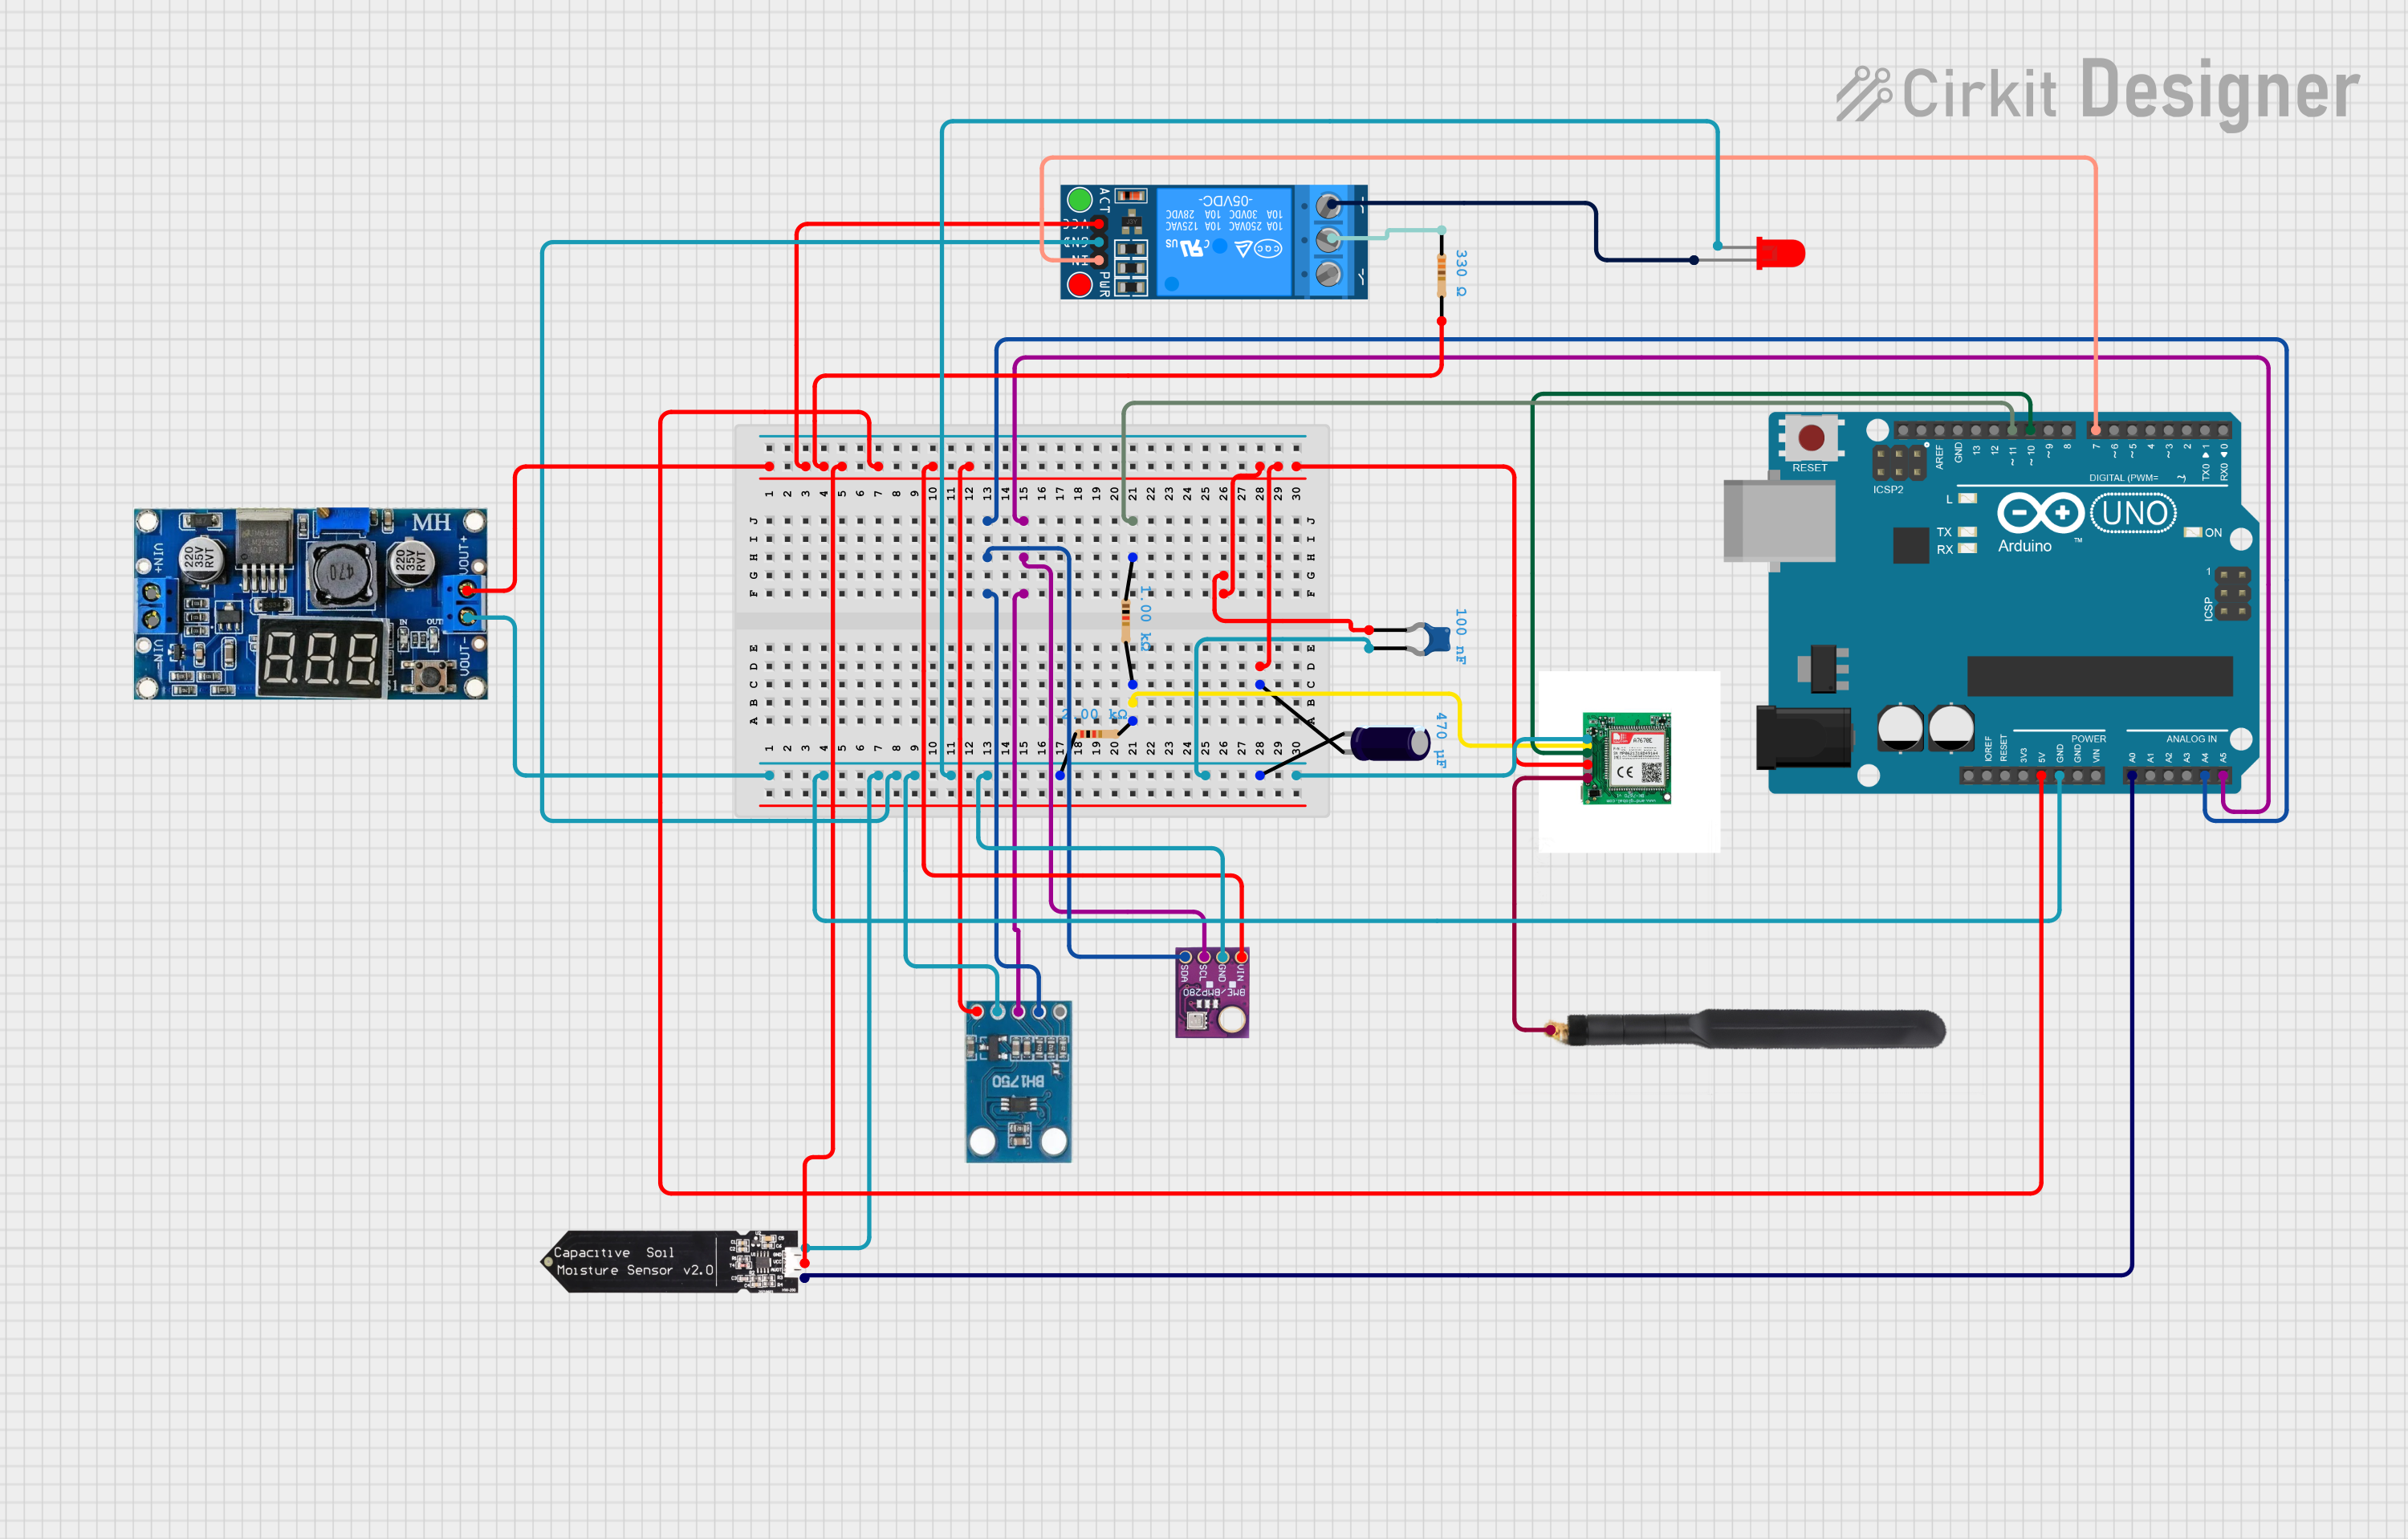
\includegraphics[width=\textwidth]{figs/esquema_estacion_TierraViva.png}
\caption{Esquema de conexión de una estación de campo de TierraViva. En la fase de prueba se representa un LED como carga de verificación; en el montaje final se sustituye por la bomba de agua de 12 V controlada mediante relé.}
\label{fig:esquema_estacion_tierraviva}
\end{figure}
\chapter{Diagramas de flujo y secuencias de funcionamiento}
\label{anexo:diagramas_flujo_funcionamiento}

Este anexo resume los principales flujos de funcionamiento de TierraViva. Su finalidad es mostrar cómo se comporta el sistema durante una ejecución normal y ante situaciones de seguridad, sin repetir el detalle de instalación, estructura de ThingSpeak o referencia de la API, que se documentan en anexos específicos.

\section{Flujo general del sistema}

La Figura~\ref{fig:flujo_general_tierraviva} muestra el recorrido completo de la información desde la estación remota hasta el usuario.

\begin{figure}[H]
    \centering
    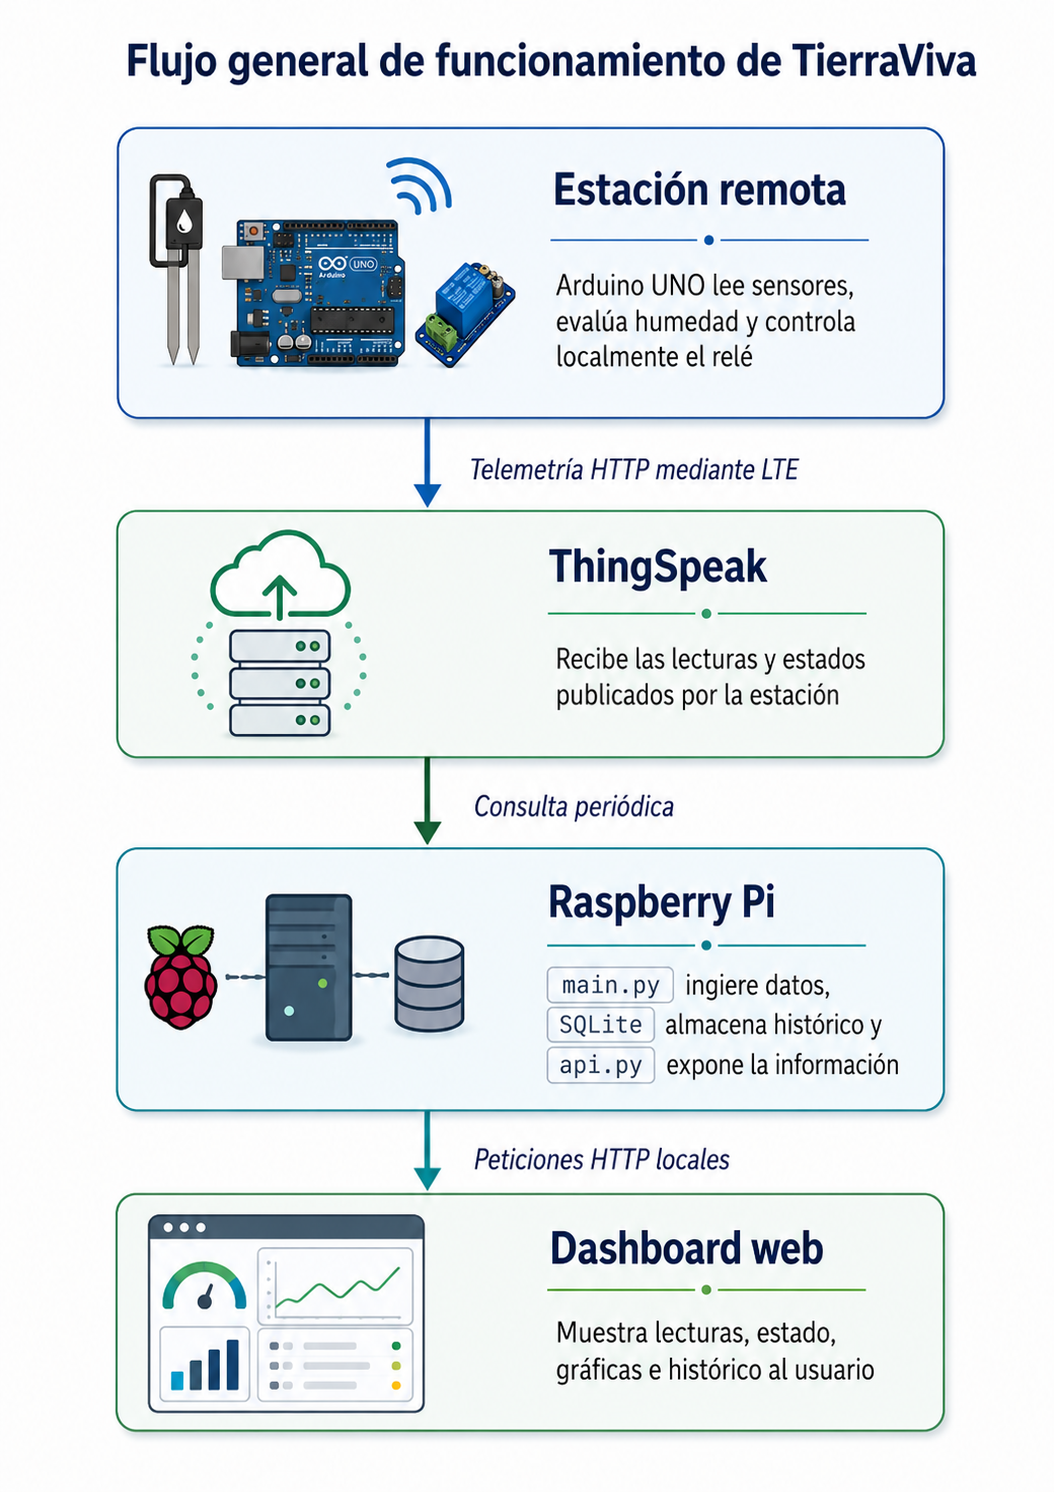
\includegraphics[width=0.5\textwidth]{figs_png/flujo_general_tierraviva.png}
    \caption{Flujo general de funcionamiento de TierraViva.}
    \label{fig:flujo_general_tierraviva}
\end{figure}

La estación concentra la medición, la decisión local y la actuación segura. ThingSpeak actúa como capa intermedia de telemetría, mientras que la Raspberry Pi se encarga de supervisar, almacenar y mostrar los datos.

\section{Ciclo de funcionamiento de la estación}

La Figura~\ref{fig:ciclo_estacion_tierraviva} resume el ciclo ejecutado por la estación remota.

\begin{figure}[H]
    \centering
    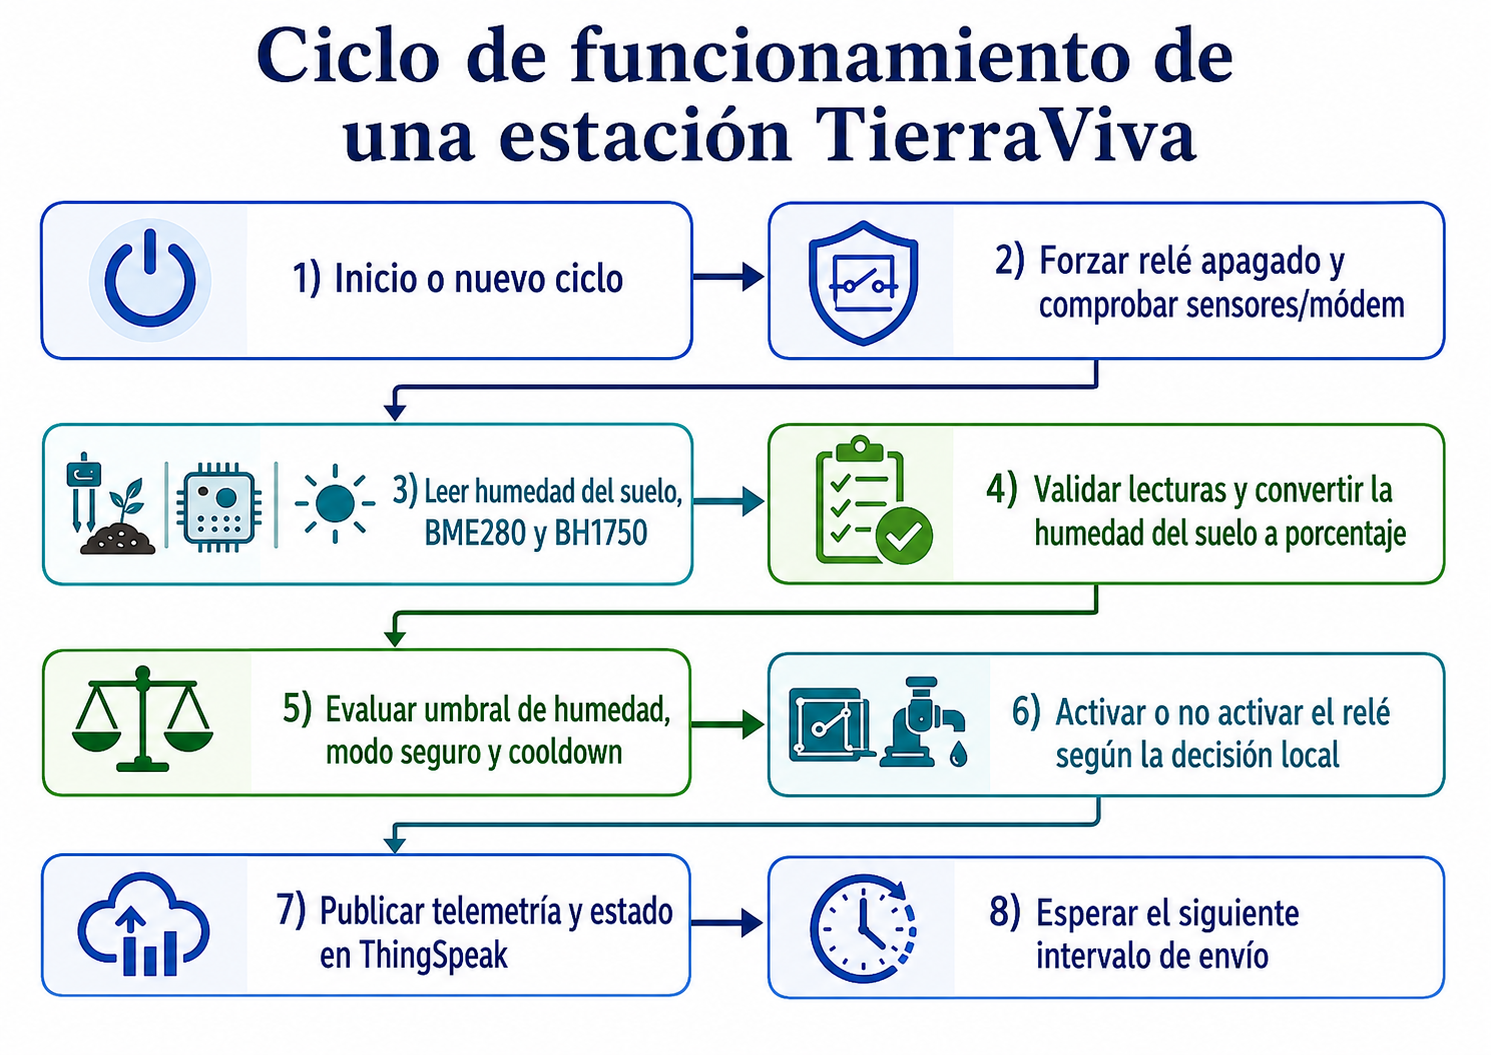
\includegraphics[width=\textwidth]{figs_png/ciclo_estacion_tierraviva.png}
        \caption{Ciclo de funcionamiento de una estación TierraViva.}
    \label{fig:ciclo_estacion_tierraviva}
\end{figure}

El relé se fuerza a estado apagado durante el arranque y la actuación se limita temporalmente mediante \textit{firmware}. Esta decisión reduce el riesgo de activaciones no deseadas.

\section{Decisión local de riego}

La Figura~\ref{fig:decision_local_riego_resumida} muestra la lógica principal de decisión de riego ejecutada en Arduino.

\begin{figure}[H]
    \centering
    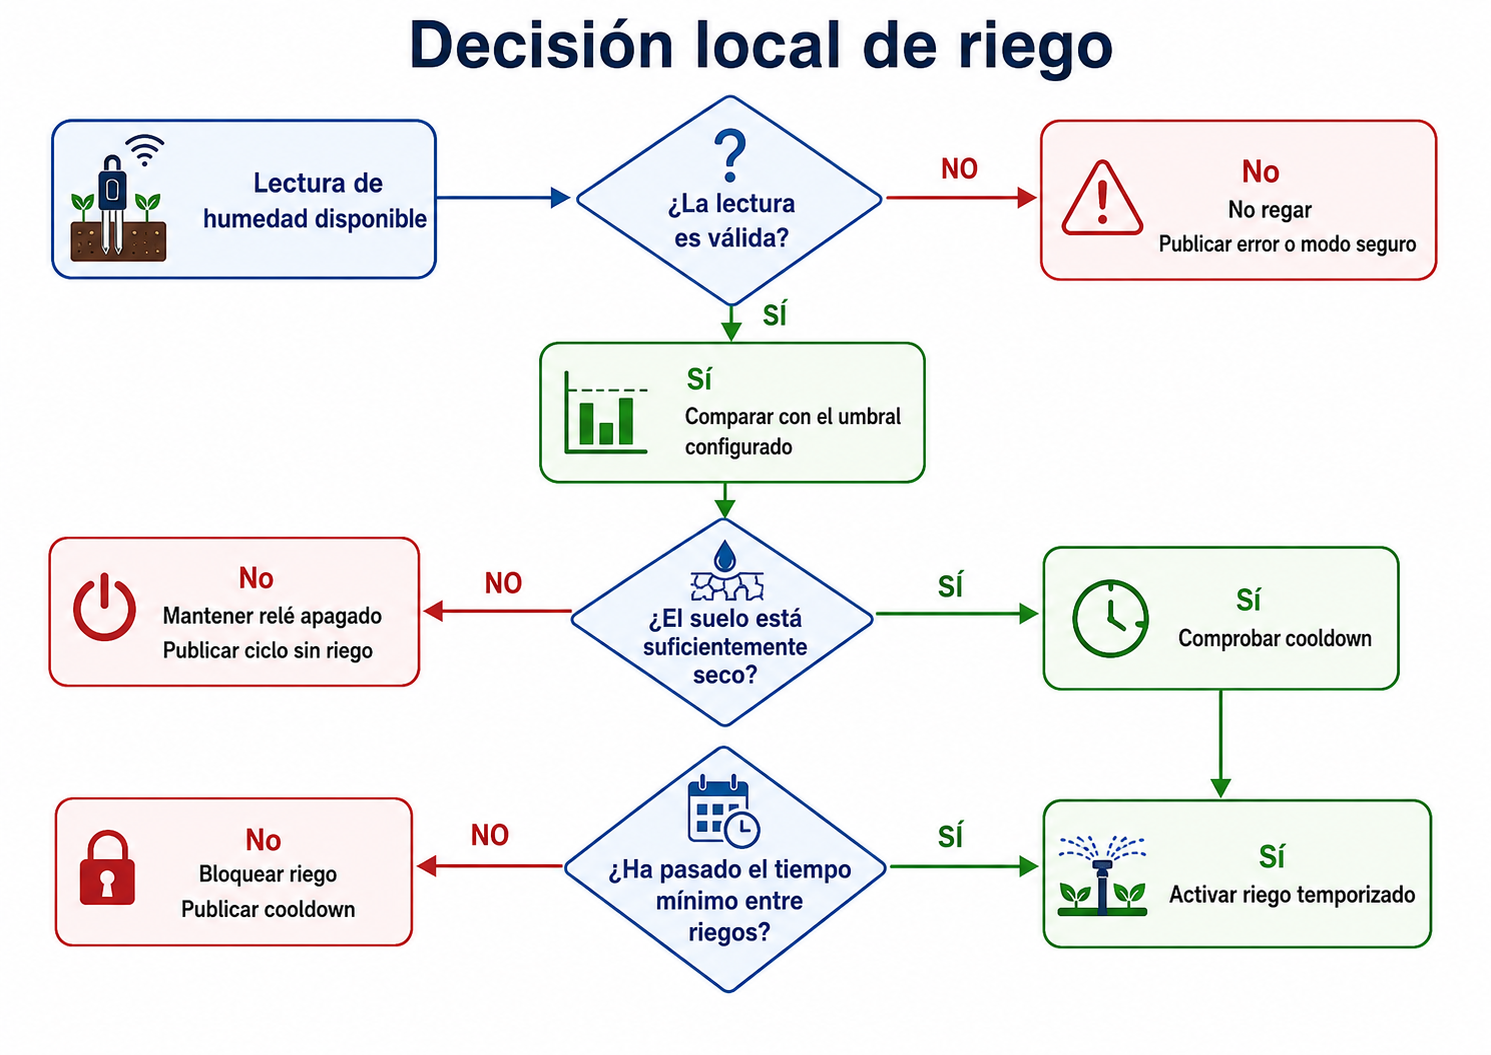
\includegraphics[width=0.75\textwidth]{figs_png/decision_local_riego_resumida.png}
        \caption{Flujo resumido de decisión local de riego.}
    \label{fig:decision_local_riego_resumida}
\end{figure}

La respuesta segura ante lectura inválida, error o \textit{cooldown} es mantener la bomba apagada.

\section{Supervisión en Raspberry Pi}

La Figura~\ref{fig:flujo_supervision_raspberry} resume el flujo seguido por la Raspberry Pi una vez que la estación ha publicado datos en ThingSpeak.

\begin{figure}[H]
    \centering
    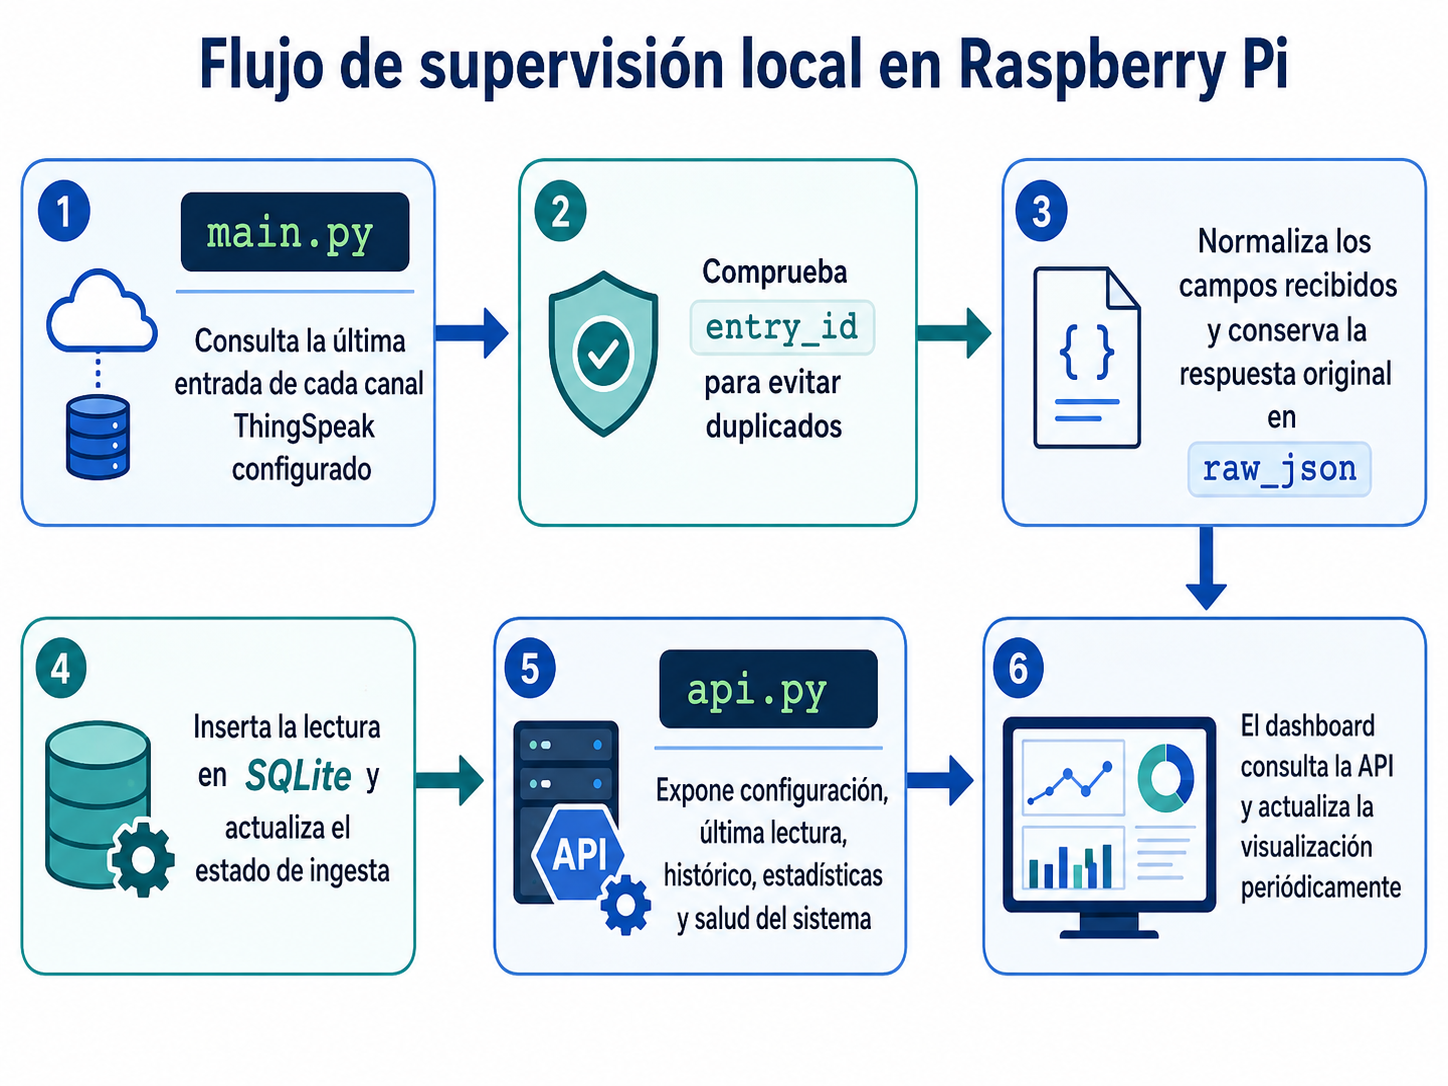
\includegraphics[width=0.7\textwidth]{figs_png/flujo_supervision_raspberry.png}
        \caption{Flujo de supervisión local en Raspberry Pi.}
    \label{fig:flujo_supervision_raspberry}
\end{figure}
    
Este flujo deja claro que la Raspberry Pi trabaja sobre datos publicados y almacenados. No se conecta físicamente a las estaciones ni acciona directamente el relé.

\section{Flujo ante fallos}

La Figura~\ref{fig:flujo_fallos_resumido} resume la respuesta esperada ante fallos relevantes.

\begin{figure}[H]
    \centering
    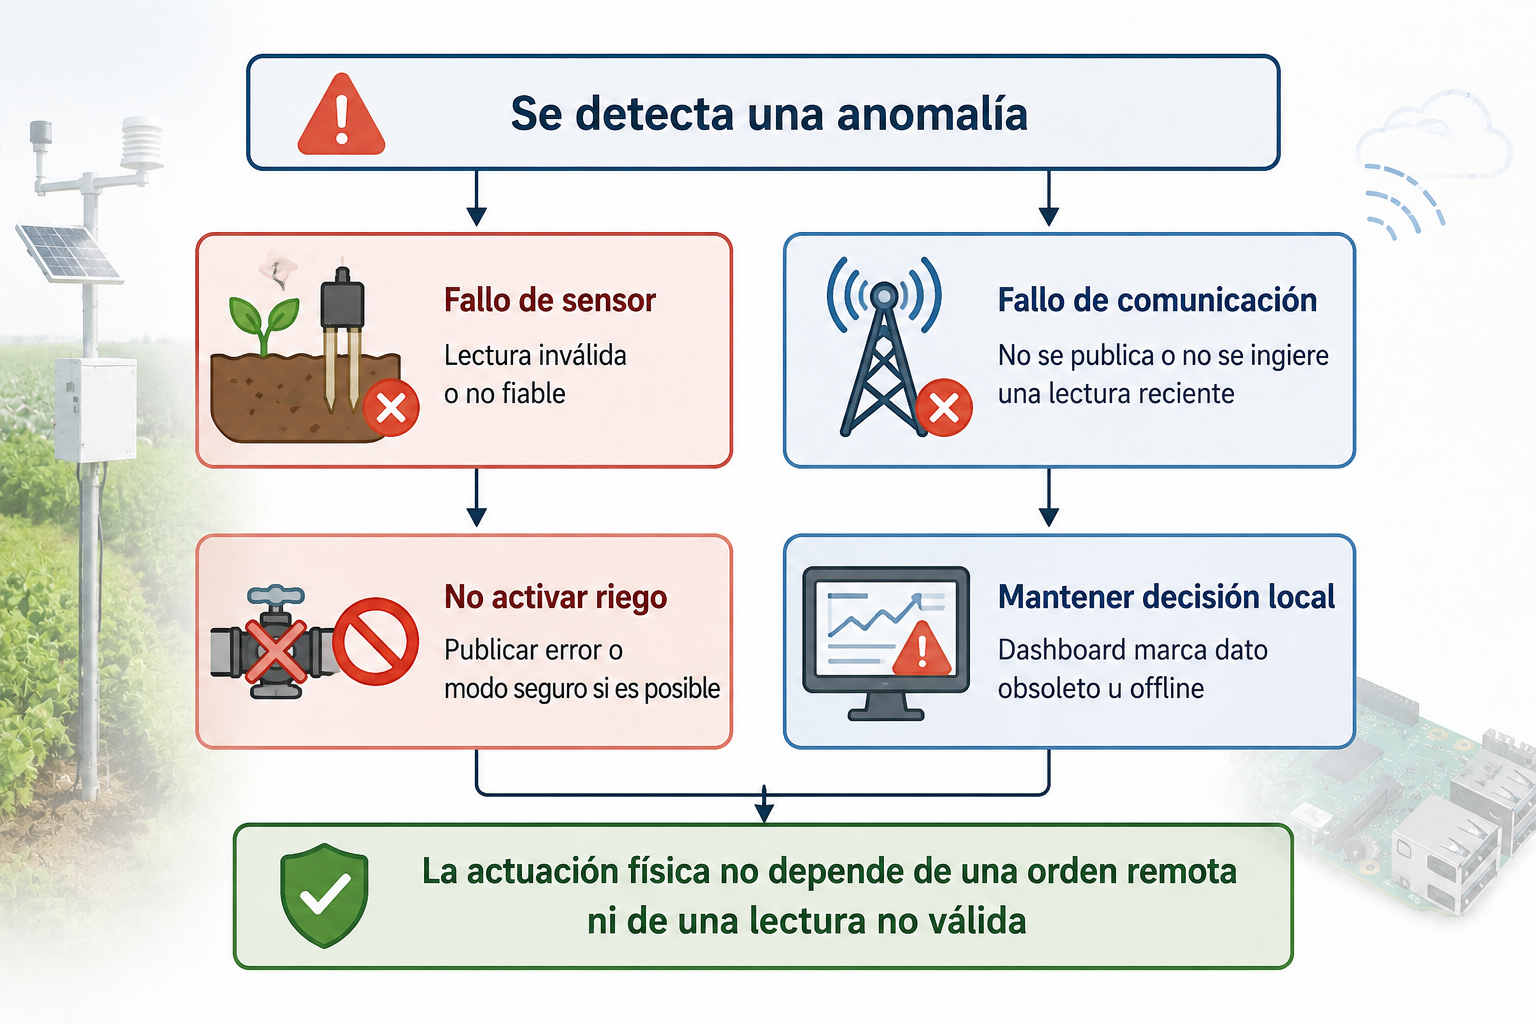
\includegraphics[width=0.7\textwidth]{figs_png/flujo_fallos_resumido.png}
        \caption{Flujo resumido ante fallos de sensor o comunicación.}
    \label{fig:flujo_fallos_resumido}
\end{figure}

La prioridad del sistema ante condiciones no fiables es mantener el estado seguro: relé apagado, riego no repetido y actuación limitada temporalmente.

\section{Secuencia extremo a extremo}

La Tabla~\ref{tab:secuencia_extremo_extremo_resumida} sintetiza la secuencia completa desde la medida física hasta la visualización.

\begin{table}[H]
\centering
\renewcommand{\arraystretch}{1.22}
\small
\begin{tabular}{|p{0.10\textwidth}|p{0.26\textwidth}|p{0.46\textwidth}|}
\hline
\rowcolor{gray!20}
\textbf{Paso} & \textbf{Elemento} & \textbf{Acción realizada} \\
\hline
1 & Sensores & Miden humedad del suelo, temperatura, humedad ambiental, luminosidad y presión. \\
\hline
2 & Arduino UNO & Valida lecturas y evalúa la lógica local de riego. \\
\hline
3 & Relé y bomba & Ejecutan el riego únicamente si se cumplen las condiciones y durante un tiempo limitado. \\
\hline
4 & A7670E-LASA & Publica telemetría y estado en ThingSpeak mediante LTE/HTTP. \\
\hline
5 & ThingSpeak & Almacena la entrada y asigna un \texttt{entry\_id}. \\
\hline
6 & Raspberry Pi & Recupera lecturas nuevas, evita duplicados y las guarda en SQLite. \\
\hline
7 & API & Expone los datos almacenados mediante \textit{endpoints} HTTP. \\
\hline
8 & \textit{Dashboard} & Muestra lecturas, estados, gráficas e histórico al usuario. \\
\hline
\end{tabular}
\caption{Secuencia extremo a extremo de TierraViva.}
\label{tab:secuencia_extremo_extremo_resumida}
\end{table}

\section{Responsabilidades por bloque}

La Tabla~\ref{tab:responsabilidades_bloques_resumida} resume las responsabilidades principales de cada capa del sistema.

\begin{table}[H]
\centering
\renewcommand{\arraystretch}{1.22}
\small
\begin{tabular}{|p{0.24\textwidth}|p{0.44\textwidth}|p{0.22\textwidth}|}
\hline
\rowcolor{gray!20}
\textbf{Bloque} & \textbf{Responsabilidad principal} & \textbf{Actúa físicamente} \\
\hline
Sensores & Medir variables del suelo y del entorno. & No \\
\hline
Arduino UNO & Leer sensores, validar datos, decidir riego y controlar el relé. & Sí \\
\hline
Relé y bomba & Ejecutar físicamente el riego cuando el \textit{firmware} lo permite. & Sí \\
\hline
A7670E-LASA & Enviar telemetría mediante LTE. & No \\
\hline
ThingSpeak & Recibir y conservar lecturas publicadas por las estaciones. & No \\
\hline
Raspberry Pi & Ingerir, almacenar y servir datos al \textit{dashboard}. & No \\
\hline
API FastAPI & Exponer lecturas, histórico, estadísticas y estado. & No \\
\hline
\textit{Dashboard} & Presentar información al usuario. & No \\
\hline
\end{tabular}
\caption{Responsabilidades principales de los bloques de TierraViva.}
\label{tab:responsabilidades_bloques_resumida}
\end{table}

\chapter{Estructura de canales ThingSpeak y codificación de estados}
\label{anexo:estructura_thingspeak_estados}

Este anexo documenta el contrato de datos utilizado por TierraViva en ThingSpeak. Su finalidad es fijar qué publica la estación remota en cada campo del canal, cómo se interpretan los estados operativos y qué correspondencia existe entre la telemetría enviada por Arduino y los nombres internos utilizados por la Raspberry Pi.

\section{Papel de ThingSpeak}

ThingSpeak cumple una función concreta dentro de TierraViva: recibir la telemetría publicada por las estaciones y permitir su consulta posterior desde la Raspberry Pi. Esta decisión simplifica la comunicación entre la estación de campo y el nodo local de supervisión, ya que la estación solo necesita publicar datos y no mantener una conexión directa con la Raspberry Pi.

El riego se decide en el firmware de la estación. Por tanto, ThingSpeak no controla la bomba, no modifica umbrales y no envía comandos a Arduino.

\section{Separación por estaciones}

Para evitar mezclar datos de distintas ubicaciones, cada estación debe utilizar un canal ThingSpeak independiente. En la configuración prevista se contemplan las estaciones \texttt{A} y \texttt{B}.

\begin{table}[H]
\centering
\renewcommand{\arraystretch}{1.25}
\small
\begin{tabular}{|p{0.22\textwidth}|p{0.32\textwidth}|p{0.32\textwidth}|}
\hline
\rowcolor{gray!20}
\textbf{Estación} & \textbf{Variable de canal} & \textbf{Uso previsto} \\
\hline
\texttt{A} & \texttt{THINGSPEAK\_CHANNEL\_A} & Canal asociado a la primera estación remota. \\
\hline
\texttt{B} & \texttt{THINGSPEAK\_CHANNEL\_B} & Canal asociado a la segunda estación remota. \\
\hline
\end{tabular}
\caption{Separación lógica de estaciones mediante canales ThingSpeak.}
\label{tab:canales_thingspeak_estaciones}
\end{table}

La Raspberry Pi recorre las estaciones configuradas en \texttt{STATIONS} y consulta el canal correspondiente a cada una. Si una estación no tiene canal definido, se ignora durante la ingesta.

\section{Estructura de campos}

Cada canal de ThingSpeak dispone de ocho campos. TierraViva utiliza los cinco primeros para variables físicas y los tres últimos para estado operativo de la estación.

\begin{table}[H]
\centering
\renewcommand{\arraystretch}{1.25}
\small
\begin{tabular}{|p{0.14\textwidth}|p{0.26\textwidth}|p{0.44\textwidth}|}
\hline
\rowcolor{gray!20}
\textbf{Campo} & \textbf{Nombre interno} & \textbf{Descripción} \\
\hline
\texttt{field1} & \texttt{soil\_moisture\_pct} & Humedad del suelo expresada en porcentaje. Es la variable principal para la decisión local de riego. \\
\hline
\texttt{field2} & \texttt{temperature\_c} & Temperatura ambiente medida por el BME280, expresada en grados Celsius. \\
\hline
\texttt{field3} & \texttt{humidity\_pct} & Humedad relativa ambiental medida por el BME280. \\
\hline
\texttt{field4} & \texttt{light\_lux} & Luminosidad medida por el BH1750, expresada en lux. \\
\hline
\texttt{field5} & \texttt{pressure\_hpa} & Presión atmosférica medida por el BME280, expresada en hPa. \\
\hline
\texttt{field6} & \texttt{relay\_state} & Estado del relé publicado por la estación: \texttt{0} apagado, \texttt{1} activo. \\
\hline
\texttt{field7} & \texttt{system\_event} & Código de evento del sistema: reposo, modo seguro, riego, error o cooldown. \\
\hline
\texttt{field8} & \texttt{debug\_code} & Código auxiliar de diagnóstico utilizado para depuración e interpretación del estado. \\
\hline
\end{tabular}
\caption{Estructura de campos utilizada en los canales ThingSpeak de TierraViva.}
\label{tab:estructura_campos_thingspeak}
\end{table}

Esta estructura permite que cada entrada de ThingSpeak contenga una fotografía completa del estado de la estación: condiciones medidas, estado del relé y motivo de la decisión tomada por el firmware.

\section{Formato de publicación}

La estación construye una petición HTTP de actualización del canal utilizando la clave de escritura y los ocho campos definidos. De forma conceptual, la petición tiene la siguiente estructura:

\begin{verbatim}
http://api.thingspeak.com/update?
    api_key=<WRITE_API_KEY>
    &field1=<humedad_suelo>
    &field2=<temperatura>
    &field3=<humedad_ambiental>
    &field4=<luminosidad>
    &field5=<presion>
    &field6=<estado_rele>
    &field7=<evento_sistema>
    &field8=<codigo_debug>
\end{verbatim}

Las claves reales no deben aparecer en la memoria, en capturas ni en el repositorio. En la documentación se representan mediante marcadores como \texttt{<WRITE\_API\_KEY>}.

\section{Codificación del estado del relé}

El campo \texttt{field6} indica el estado del relé en el momento de la publicación.

\begin{table}[H]
\centering
\renewcommand{\arraystretch}{1.25}
\small
\begin{tabular}{|p{0.18\textwidth}|p{0.24\textwidth}|p{0.44\textwidth}|}
\hline
\rowcolor{gray!20}
\textbf{Valor} & \textbf{Estado} & \textbf{Interpretación} \\
\hline
\texttt{0} & Relé apagado & La bomba no debería estar alimentada en el momento de la lectura publicada. \\
\hline
\texttt{1} & Relé activo & La estación informa de que el relé está activo y la bomba puede estar funcionando. \\
\hline
Sin dato & Desconocido & No se ha recibido un valor válido para el estado del relé. \\
\hline
\end{tabular}
\caption{Interpretación del campo \texttt{relay\_state}.}
\label{tab:interpretacion_relay_state}
\end{table}

Este valor representa el estado publicado en la última telemetría disponible. Si la lectura es antigua, el estado físico real puede haber cambiado.

\section{Codificación de eventos de sistema}

El campo \texttt{field7} contiene el evento principal de la estación durante el ciclo de funcionamiento. La Tabla \ref{tab:codificacion_system_event} resume los códigos utilizados.

\begin{table}[H]
\centering
\renewcommand{\arraystretch}{1.25}
\small
\begin{tabular}{|p{0.16\textwidth}|p{0.26\textwidth}|p{0.44\textwidth}|}
\hline
\rowcolor{gray!20}
\textbf{Código} & \textbf{Etiqueta} & \textbf{Significado} \\
\hline
\texttt{100} & \texttt{idle} & Estación en reposo. No hay riego activo en el ciclo actual. \\
\hline
\texttt{206} & \texttt{safe mode} & La estación se encuentra en modo seguro. Se aplican condiciones más conservadoras antes de actuar. \\
\hline
\texttt{210} & \texttt{riego ON} & La estación ha activado el riego. \\
\hline
\texttt{211} & \texttt{riego OFF} & La estación ha finalizado el riego y ha apagado el relé. \\
\hline
\texttt{400} & \texttt{error} & Se ha detectado un error relevante, normalmente asociado a sensores o lecturas no válidas. \\
\hline
\texttt{429} & \texttt{cooldown} & La estación ha bloqueado una activación porque no ha finalizado el tiempo mínimo entre riegos. \\
\hline
\end{tabular}
\caption{Codificación del campo \texttt{system\_event}.}
\label{tab:codificacion_system_event}
\end{table}

Este campo permite distinguir si la estación está en reposo, en modo seguro, regando, finalizando un riego o bloqueando una activación por seguridad.

\section{Codificación de diagnóstico}

El campo \texttt{field8} contiene un código auxiliar de diagnóstico. Este valor complementa al evento principal y facilita la depuración.

\begin{table}[H]
\centering
\renewcommand{\arraystretch}{1.25}
\small
\begin{tabular}{|p{0.16\textwidth}|p{0.26\textwidth}|p{0.44\textwidth}|}
\hline
\rowcolor{gray!20}
\textbf{Código} & \textbf{Etiqueta} & \textbf{Significado} \\
\hline
\texttt{200} & \texttt{OK} & Funcionamiento correcto en el ciclo actual. \\
\hline
\texttt{204} & \texttt{no riego} & No se ha activado el riego porque no se cumplen las condiciones necesarias. \\
\hline
\texttt{206} & \texttt{modo seguro} & La estación está operando en modo seguro. \\
\hline
\texttt{400} & \texttt{error} & Se ha detectado un error o una lectura no válida. \\
\hline
\texttt{429} & \texttt{cooldown} & El riego se ha bloqueado por periodo de seguridad entre activaciones. \\
\hline
\end{tabular}
\caption{Codificación del campo \texttt{debug\_code}.}
\label{tab:codificacion_debug_code}
\end{table}

La diferencia entre \texttt{system\_event} y \texttt{debug\_code} es que el primero describe el evento principal del sistema, mientras que el segundo resume el resultado o condición auxiliar del ciclo.

\section{Interpretación conjunta de estados}

La interpretación más útil se obtiene combinando \texttt{relay\_state}, \texttt{system\_event} y \texttt{debug\_code}.

\begin{table}[H]
\centering
\renewcommand{\arraystretch}{1.25}
\scriptsize
\begin{tabular}{|p{0.18\textwidth}|p{0.18\textwidth}|p{0.18\textwidth}|p{0.34\textwidth}|}
\hline
\rowcolor{gray!20}
\textbf{\texttt{relay\_state}} & \textbf{\texttt{system\_event}} & \textbf{\texttt{debug\_code}} & \textbf{Interpretación} \\
\hline
\texttt{0} & \texttt{100} & \texttt{204} & Estación en reposo. No se activa el riego porque no se cumplen las condiciones necesarias. \\
\hline
\texttt{0} & \texttt{206} & \texttt{206} & Estación en modo seguro. El sistema aplica criterios más conservadores. \\
\hline
\texttt{1} & \texttt{210} & \texttt{200} & Riego activo. El relé está activado durante el intervalo configurado. \\
\hline
\texttt{0} & \texttt{211} & \texttt{200} & Riego finalizado. El relé ha vuelto a estado apagado. \\
\hline
\texttt{0} & \texttt{400} & \texttt{400} & Error de sensores o lectura no válida. La respuesta segura es no activar el riego. \\
\hline
\texttt{0} & \texttt{429} & \texttt{429} & Riego bloqueado por cooldown. La estación evita una activación demasiado cercana a la anterior. \\
\hline
\end{tabular}
\caption{Interpretación conjunta de estado de relé, evento y diagnóstico.}
\label{tab:relacion_evento_diagnostico_actuacion}
\end{table}

Esta tabla permite que los valores publicados en ThingSpeak se puedan traducir a estados comprensibles.

\section{Normalización en Raspberry Pi}

El ingestor \texttt{main.py} consulta la última entrada del canal ThingSpeak y traduce los campos genéricos \texttt{field1}--\texttt{field8} a nombres internos. La normalización aplicada se resume en la Tabla \ref{tab:normalizacion_campos_thingspeak}.

\begin{table}[H]
\centering
\renewcommand{\arraystretch}{1.25}
\small
\begin{tabular}{|p{0.20\textwidth}|p{0.32\textwidth}|p{0.32\textwidth}|}
\hline
\rowcolor{gray!20}
\textbf{Campo recibido} & \textbf{Nombre interno} & \textbf{Conversión esperada} \\
\hline
\texttt{entry\_id} & \texttt{entry\_id} & Entero. \\
\hline
\texttt{created\_at} & \texttt{created\_at} & Fecha original de ThingSpeak. \\
\hline
\texttt{field1} & \texttt{soil\_moisture\_pct} & Número real. \\
\hline
\texttt{field2} & \texttt{temperature\_c} & Número real. \\
\hline
\texttt{field3} & \texttt{humidity\_pct} & Número real. \\
\hline
\texttt{field4} & \texttt{light\_lux} & Número real. \\
\hline
\texttt{field5} & \texttt{pressure\_hpa} & Número real. \\
\hline
\texttt{field6} & \texttt{relay\_state} & Entero. \\
\hline
\texttt{field7} & \texttt{system\_event} & Texto o código numérico. \\
\hline
\texttt{field8} & \texttt{debug\_code} & Texto o código numérico. \\
\hline
\end{tabular}
\caption{Normalización de campos recibidos desde ThingSpeak.}
\label{tab:normalizacion_campos_thingspeak}
\end{table}

El valor \texttt{entry\_id} se utiliza para evitar insertar varias veces la misma entrada. Si el identificador recibido coincide con el último procesado para esa estación, la lectura se considera duplicada y se ignora.

\section{Persistencia y trazabilidad}

Las lecturas se almacenan en la tabla \texttt{readings} de SQLite. Las variables principales se insertan como columnas normalizadas, mientras que la respuesta original de ThingSpeak se conserva en \texttt{raw\_json} para mantener trazabilidad.

Esto es relevante para los campos de estado: \texttt{relay\_state}, \texttt{system\_event} y \texttt{debug\_code} se normalizan durante la ingesta y se registran en los logs, pero pueden conservarse principalmente dentro de \texttt{raw\_json} si no se insertan explícitamente como columnas. Por ello, cualquier visualización o depuración debe contemplar la lectura de esos valores desde la respuesta original cuando sea necesario.

\section{Errores habituales de configuración}

\begin{table}[H]
\centering
\renewcommand{\arraystretch}{1.25}
\scriptsize
\begin{tabular}{|p{0.30\textwidth}|p{0.28\textwidth}|p{0.30\textwidth}|}
\hline
\rowcolor{gray!20}
\textbf{Error} & \textbf{Efecto observable} & \textbf{Corrección recomendada} \\
\hline
Clave de escritura incorrecta & El canal no recibe nuevas entradas. & Revisar \texttt{THINGSPEAK\_API\_KEY} en el firmware. \\
\hline
Canal incorrecto en Raspberry Pi & Se consulta un canal que no corresponde a la estación. & Revisar \texttt{THINGSPEAK\_CHANNEL\_A/B}. \\
\hline
Clave de lectura incorrecta & La Raspberry Pi no puede recuperar datos si el canal es privado. & Revisar \texttt{THINGSPEAK\_READ\_KEY\_A/B}. \\
\hline
Campos desordenados & El dashboard o la API interpretan valores incorrectos. & Mantener fija la correspondencia \texttt{field1}--\texttt{field8}. \\
\hline
Sin nuevas entradas & La API mantiene la última lectura disponible o muestra datos antiguos. & Revisar estación, LTE, ThingSpeak, ingestor y alimentación. \\
\hline
Publicación demasiado frecuente & ThingSpeak puede no aceptar todas las actualizaciones. & Respetar el intervalo de envío configurado en el firmware. \\
\hline
\end{tabular}
\caption{Errores habituales asociados a la configuración de ThingSpeak.}
\label{tab:errores_thingspeak}
\end{table}

\section{Limitaciones de la versión actual}

En la versión actual, ThingSpeak se utiliza únicamente para telemetría ascendente:

\begin{itemize}
    \item la estación publica datos hacia ThingSpeak;
    \item la Raspberry Pi consulta datos desde ThingSpeak;
    \item la decisión de riego se ejecuta localmente en Arduino;
    \item no se envían órdenes de riego desde el dashboard;
    \item no existe canal descendente de comandos hacia la estación.
\end{itemize}

Esta limitación es deliberada. La actuación sobre una bomba implica riesgos eléctricos e hidráulicos, por lo que la versión actual prioriza una lógica local con apagado explícito, cooldown y comportamiento seguro ante lecturas no válidas.

\section{Conclusión}

La estructura de ThingSpeak de TierraViva define un contrato de datos entre estación, plataforma IoT y Raspberry Pi. Los campos \texttt{field1}--\texttt{field5} transportan variables físicas, mientras que \texttt{field6}--\texttt{field8} describen el estado operativo de la estación.

Mantener estable esta correspondencia es esencial para que el firmware, el ingestor, la base de datos, la API y el dashboard interpreten los datos de forma coherente.

\chapter{Manual de instalación y puesta en marcha de TierraViva}
\label{anexo:manual_instalacion_sistema}

Este anexo describe el procedimiento necesario para instalar y poner en marcha TierraViva a partir del repositorio del proyecto. Su objetivo es permitir que el prototipo pueda reproducirse de forma ordenada, comprobando cada bloque antes de ejecutar una prueba completa.

El manual se centra en la instalación práctica del sistema. Los esquemas eléctricos se recogen en el Anexo~\ref{anexo:esquemas_electricos}; los flujos de funcionamiento, en el Anexo~\ref{anexo:diagramas_flujo_funcionamiento}; la estructura de ThingSpeak, en el Anexo~\ref{anexo:estructura_thingspeak_estados}; y la referencia completa de \textit{endpoints}, en el Anexo~\ref{anexo:manual_api}.

\section{Alcance}

La instalación descrita corresponde a la versión actual de TierraViva, formada por:

\begin{itemize}
    \item una o varias estaciones remotas basadas en Arduino UNO;
    \item publicación de telemetría en ThingSpeak mediante LTE;
    \item Raspberry Pi como nodo local de supervisión;
    \item base de datos SQLite;
    \item API local con FastAPI;
    \item \textit{dashboard} web accesible desde navegador.
\end{itemize}

\section{Requisitos previos}

Antes de comenzar la instalación deben estar disponibles los siguientes elementos:

\begin{itemize}
    \item repositorio del proyecto TierraViva;
    \item Raspberry Pi con Raspberry Pi OS y conexión a Internet;
    \item Arduino IDE para cargar el \textit{firmware} de estación;
    \item cuenta de ThingSpeak;
    \item un canal ThingSpeak por estación;
    \item \texttt{Channel ID}, \texttt{Read API Key} y \texttt{Write API Key} de cada canal;
    \item tarjeta SIM sin PIN activo;
    \item módulo A7670E-LASA con antena conectada;
    \item estación montada según el esquema eléctrico del Anexo~\ref{anexo:esquemas_electricos}.
\end{itemize}

Las claves reales deben mantenerse fuera de la memoria y del repositorio. En la documentación se utilizarán siempre marcadores como \texttt{<READ\_KEY\_A>} o \texttt{<WRITE\_KEY\_A>}.

\section{Preparación de ThingSpeak}

Para cada estación debe existir un canal ThingSpeak independiente. La correspondencia entre campos y variables se encuentra documentada en el Anexo~\ref{anexo:estructura_thingspeak_estados}. Como comprobación mínima, antes de integrar la estación se recomienda verificar que el canal acepta una escritura manual.

\begin{terminaloutput}
https://api.thingspeak.com/update?api_key=<WRITE_KEY>&field1=35
\end{terminaloutput}

Si la petición es correcta, ThingSpeak devuelve un número de entrada. Después debe comprobarse en el canal que se ha registrado una nueva lectura.

\section{Carga del \textit{firmware} de estación}

El \textit{firmware} de la estación se encuentra en:

\begin{terminaloutput}
Estacion/Estacion_A_final_Plus/Estacion_A_final_Plus.ino
\end{terminaloutput}

Antes de cargarlo en Arduino UNO deben revisarse, como mínimo, los siguientes parámetros:

\begin{table}[H]
\centering
\renewcommand{\arraystretch}{1.15}
\rowcolors{2}{TableRowSoft}{white}
\small

\begin{tabular}{|p{0.34\textwidth}|p{0.48\textwidth}|}
\hline
\rowcolor{URJCRed}
\TVHead{Parámetro} & \TVHead{Función} \\
\hline
\texttt{APN} & APN del operador móvil utilizado por la SIM. \\
\hline
\texttt{THINGSPEAK\_API\_KEY} & Clave de escritura del canal ThingSpeak de la estación. \\
\hline
\texttt{SOIL\_DRY} & Valor bruto del sensor en condición seca. \\
\hline
\texttt{SOIL\_WET} & Valor bruto del sensor en condición húmeda. \\
\hline
\texttt{NORMAL\_SOIL\_THRESHOLD} & Umbral de humedad usado en funcionamiento normal. \\
\hline
\texttt{SAFE\_SOIL\_THRESHOLD} & Umbral de humedad usado en modo seguro. \\
\hline
\texttt{IRRIGATION\_SECONDS} & Duración del riego local. \\
\hline
\texttt{COOLDOWN\_MS} & Tiempo mínimo entre dos riegos consecutivos. \\
\hline
\texttt{SEND\_INTERVAL\_MS} & Intervalo de publicación de telemetría. \\
\hline
\end{tabular}
\caption{Parámetros principales que deben revisarse antes de cargar el \textit{firmware}.}
\label{tab:parametros_firmware_instalacion}
\end{table}

\subsection{Librerías empleadas por el \textit{firmware}}
\label{subsec:librerias_firmware_estacion}

El \textit{firmware} de la estación remota utiliza varias librerías de Arduino y de C/C++ para gestionar la comunicación con sensores, el módem LTE y el tratamiento de cadenas. Estas dependencias permiten implementar de forma ordenada los bloques principales del \textit{sketch}: lectura I2C, comunicación serie con el A7670E-LASA, adquisición de medidas ambientales y construcción de peticiones HTTP.

\begin{table}[H]
\centering
\renewcommand{\arraystretch}{1.15}
\rowcolors{2}{TableRowSoft}{white}

\small
\begin{tabular}{|p{0.25\textwidth}|p{0.31\textwidth}|p{0.34\textwidth}|}
\hline
\rowcolor{URJCRed}
\TVHead{Librería} & \TVHead{Uso en TierraViva} & \TVHead{Motivo de utilización} \\
\hline
\texttt{SoftwareSerial} & Comunicación UART entre Arduino UNO y el módem A7670E-LASA mediante los pines \texttt{D10} y \texttt{D11}. & Permite disponer de un puerto serie adicional, manteniendo el puerto serie hardware para programación y depuración por USB. \\
\hline
\texttt{Wire} & Comunicación I2C con los sensores digitales BME280 y BH1750. & Proporciona las funciones necesarias para usar el bus I2C del Arduino UNO, asociado a los pines \texttt{A4/SDA} y \texttt{A5/SCL}. \\
\hline
\texttt{BH1750} & Lectura del sensor de luminosidad BH1750/GY-302. & Permite obtener directamente la iluminancia en lux, evitando trabajar con una lectura analógica sin escala física directa. \\
\hline
\texttt{Adafruit\_Sensor} & Capa común utilizada por sensores de la familia Adafruit. & Proporciona estructuras y tipos comunes requeridos por la librería del BME280. \\
\hline
\texttt{Adafruit\_BME280} & Lectura del sensor ambiental BME280. & Permite obtener temperatura, humedad relativa y presión atmosférica mediante I2C. \\
\hline
\texttt{string.h} & Tratamiento de cadenas en C, como búsqueda de respuestas y construcción de mensajes. & Permite usar funciones como \texttt{strstr()} y \texttt{snprintf()}, útiles para interpretar respuestas del módem y construir peticiones HTTP con buffers controlados. \\
\hline
\end{tabular}
\caption{Librerías principales utilizadas por el \textit{firmware} de estación.}
\label{tab:librerias_firmware_estacion}
\end{table}

El uso de \texttt{SoftwareSerial} requiere una consideración específica. Arduino UNO solo dispone de un puerto serie hardware, utilizado normalmente para cargar el programa y depurar mediante el monitor serie. Por ello, la comunicación con el A7670E-LASA se implementa mediante un puerto serie software en los pines \texttt{D10} y \texttt{D11}. En el montaje de TierraViva, \texttt{D10} recibe datos desde \texttt{TXD} del módem y \texttt{D11} transmite hacia \texttt{RXD} del módem mediante divisor resistivo.

Durante las pruebas se evitó utilizar velocidades elevadas en este puerto serie software. Aunque algunos módems pueden trabajar a baudios superiores, en Arduino UNO \texttt{SoftwareSerial} puede volverse inestable a velocidades altas. Por ese motivo, el \textit{firmware} se estabilizó a \texttt{9600} baudios, priorizando fiabilidad frente a velocidad de transmisión.

Las librerías \texttt{Wire}, \texttt{BH1750} y \texttt{Adafruit\_BME280} permiten integrar los sensores digitales sobre el mismo bus I2C. En la estación, el BH1750 se detectó en la dirección \texttt{0x23} y el BME280 en la dirección \texttt{0x76}, por lo que ambos pueden compartir las líneas \texttt{SDA} y \texttt{SCL} sin conflicto de direcciones.

Por último, \texttt{string.h} se utiliza para trabajar con cadenas de caracteres de forma controlada. Esta decisión es relevante en Arduino UNO porque la memoria SRAM disponible es reducida. Funciones como \texttt{snprintf()} permiten construir cadenas dentro de buffers de tamaño definido, mientras que \texttt{strstr()} permite comprobar si una respuesta del módem contiene textos como \texttt{OK} o códigos HTTP esperados.

La carga del \textit{firmware} se realiza desde Arduino IDE:

\begin{enumerate}
    \item Conectar Arduino UNO al ordenador mediante USB;
    \item Abrir el fichero \texttt{Estacion\_X\_final\_Plus.ino}, siendo \texttt{X} la letra de la estación correspondiente, por ejemplo \texttt{A} o \texttt{B};
    \item Seleccionar la placa \textit{Arduino UNO};
    \item Seleccionar el puerto serie correspondiente;
    \item Comprobar que las librerías indicadas en la Tabla~\ref{tab:librerias_firmware_estacion} están disponibles en el entorno de Arduino;
    \item Compilar el programa;
    \item Cargar el \textit{firmware};
    \item Abrir el monitor serie a \texttt{9600} baudios para comprobar sensores, módem, red LTE y publicación.
\end{enumerate}

La Figura~\ref{fig:arduino_placa_uno} muestra el procedimiento para seleccionar la placa \textit{Arduino UNO} en Arduino IDE. A continuación, la Figura~\ref{fig:arduino_puerto_usb} muestra la selección del puerto serie asociado a la placa conectada por USB.

\begin{figure}[H]
    \centering
    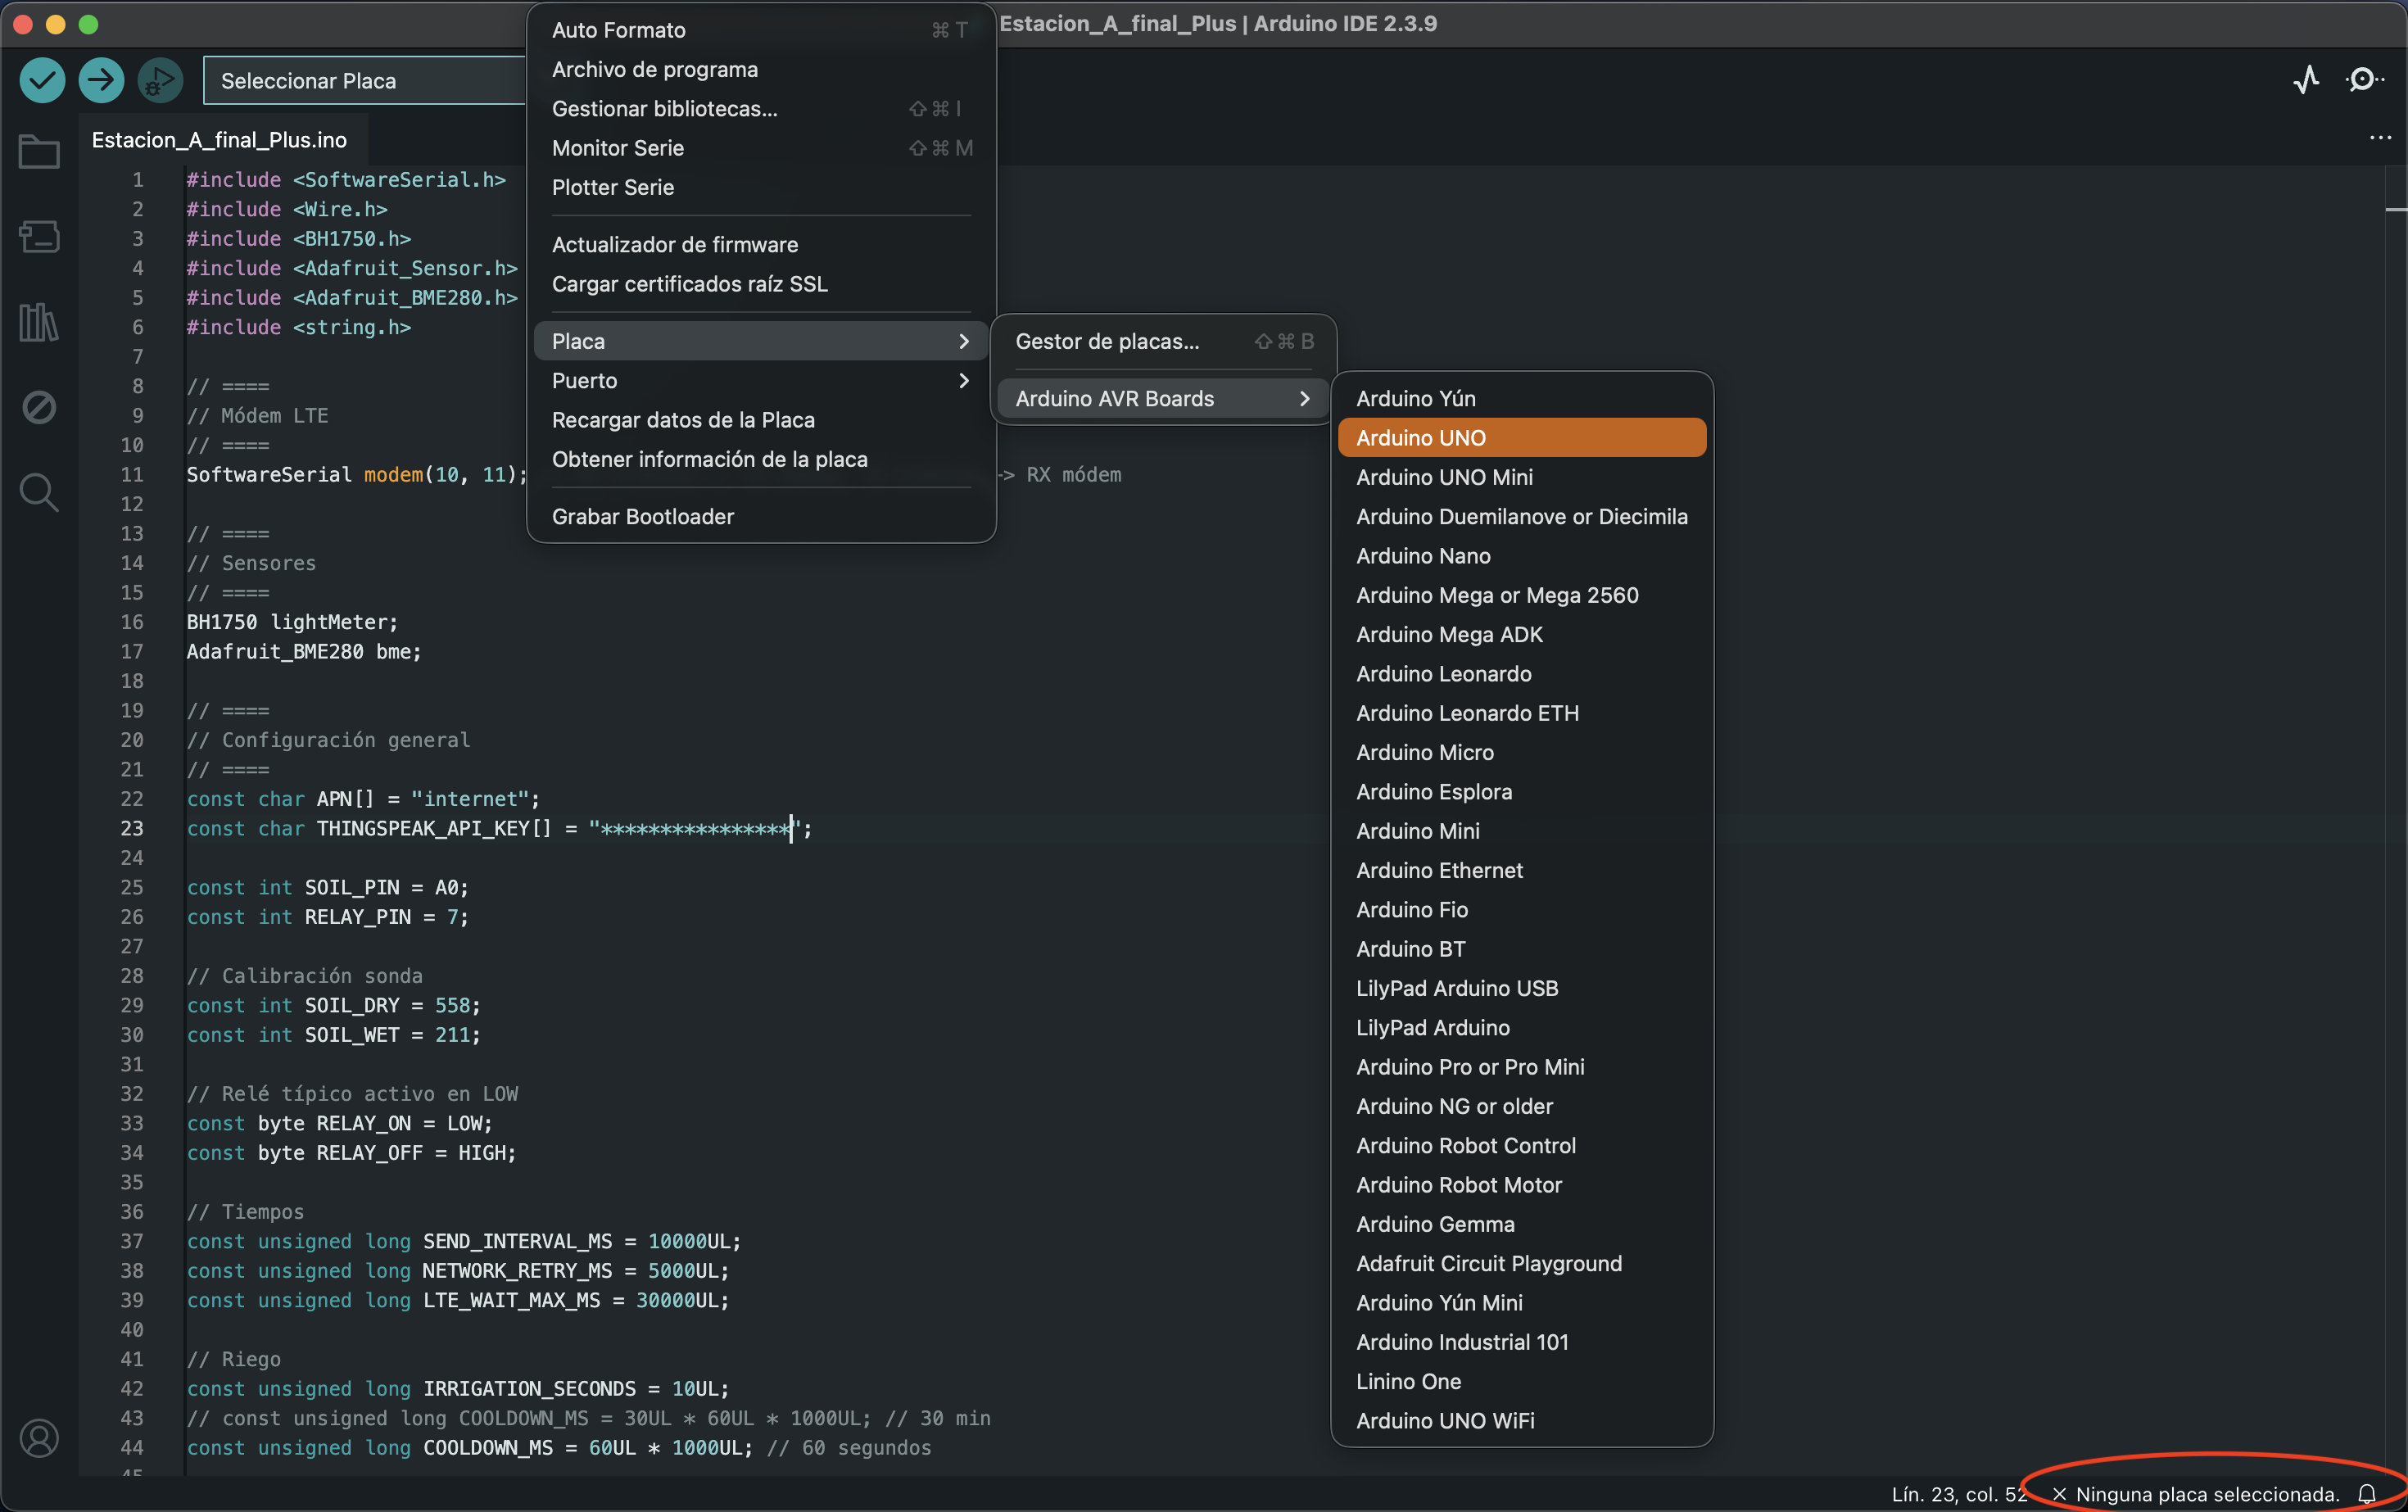
\includegraphics[width=0.92\textwidth]{figs/seleccion_placa_Arduino.png}
    \caption{Selección de la placa \textit{Arduino UNO} en Arduino IDE antes de cargar el \textit{firmware} de la estación. Captura propia.}
    \label{fig:arduino_placa_uno}
\end{figure}

\begin{figure}[H]
    \centering
    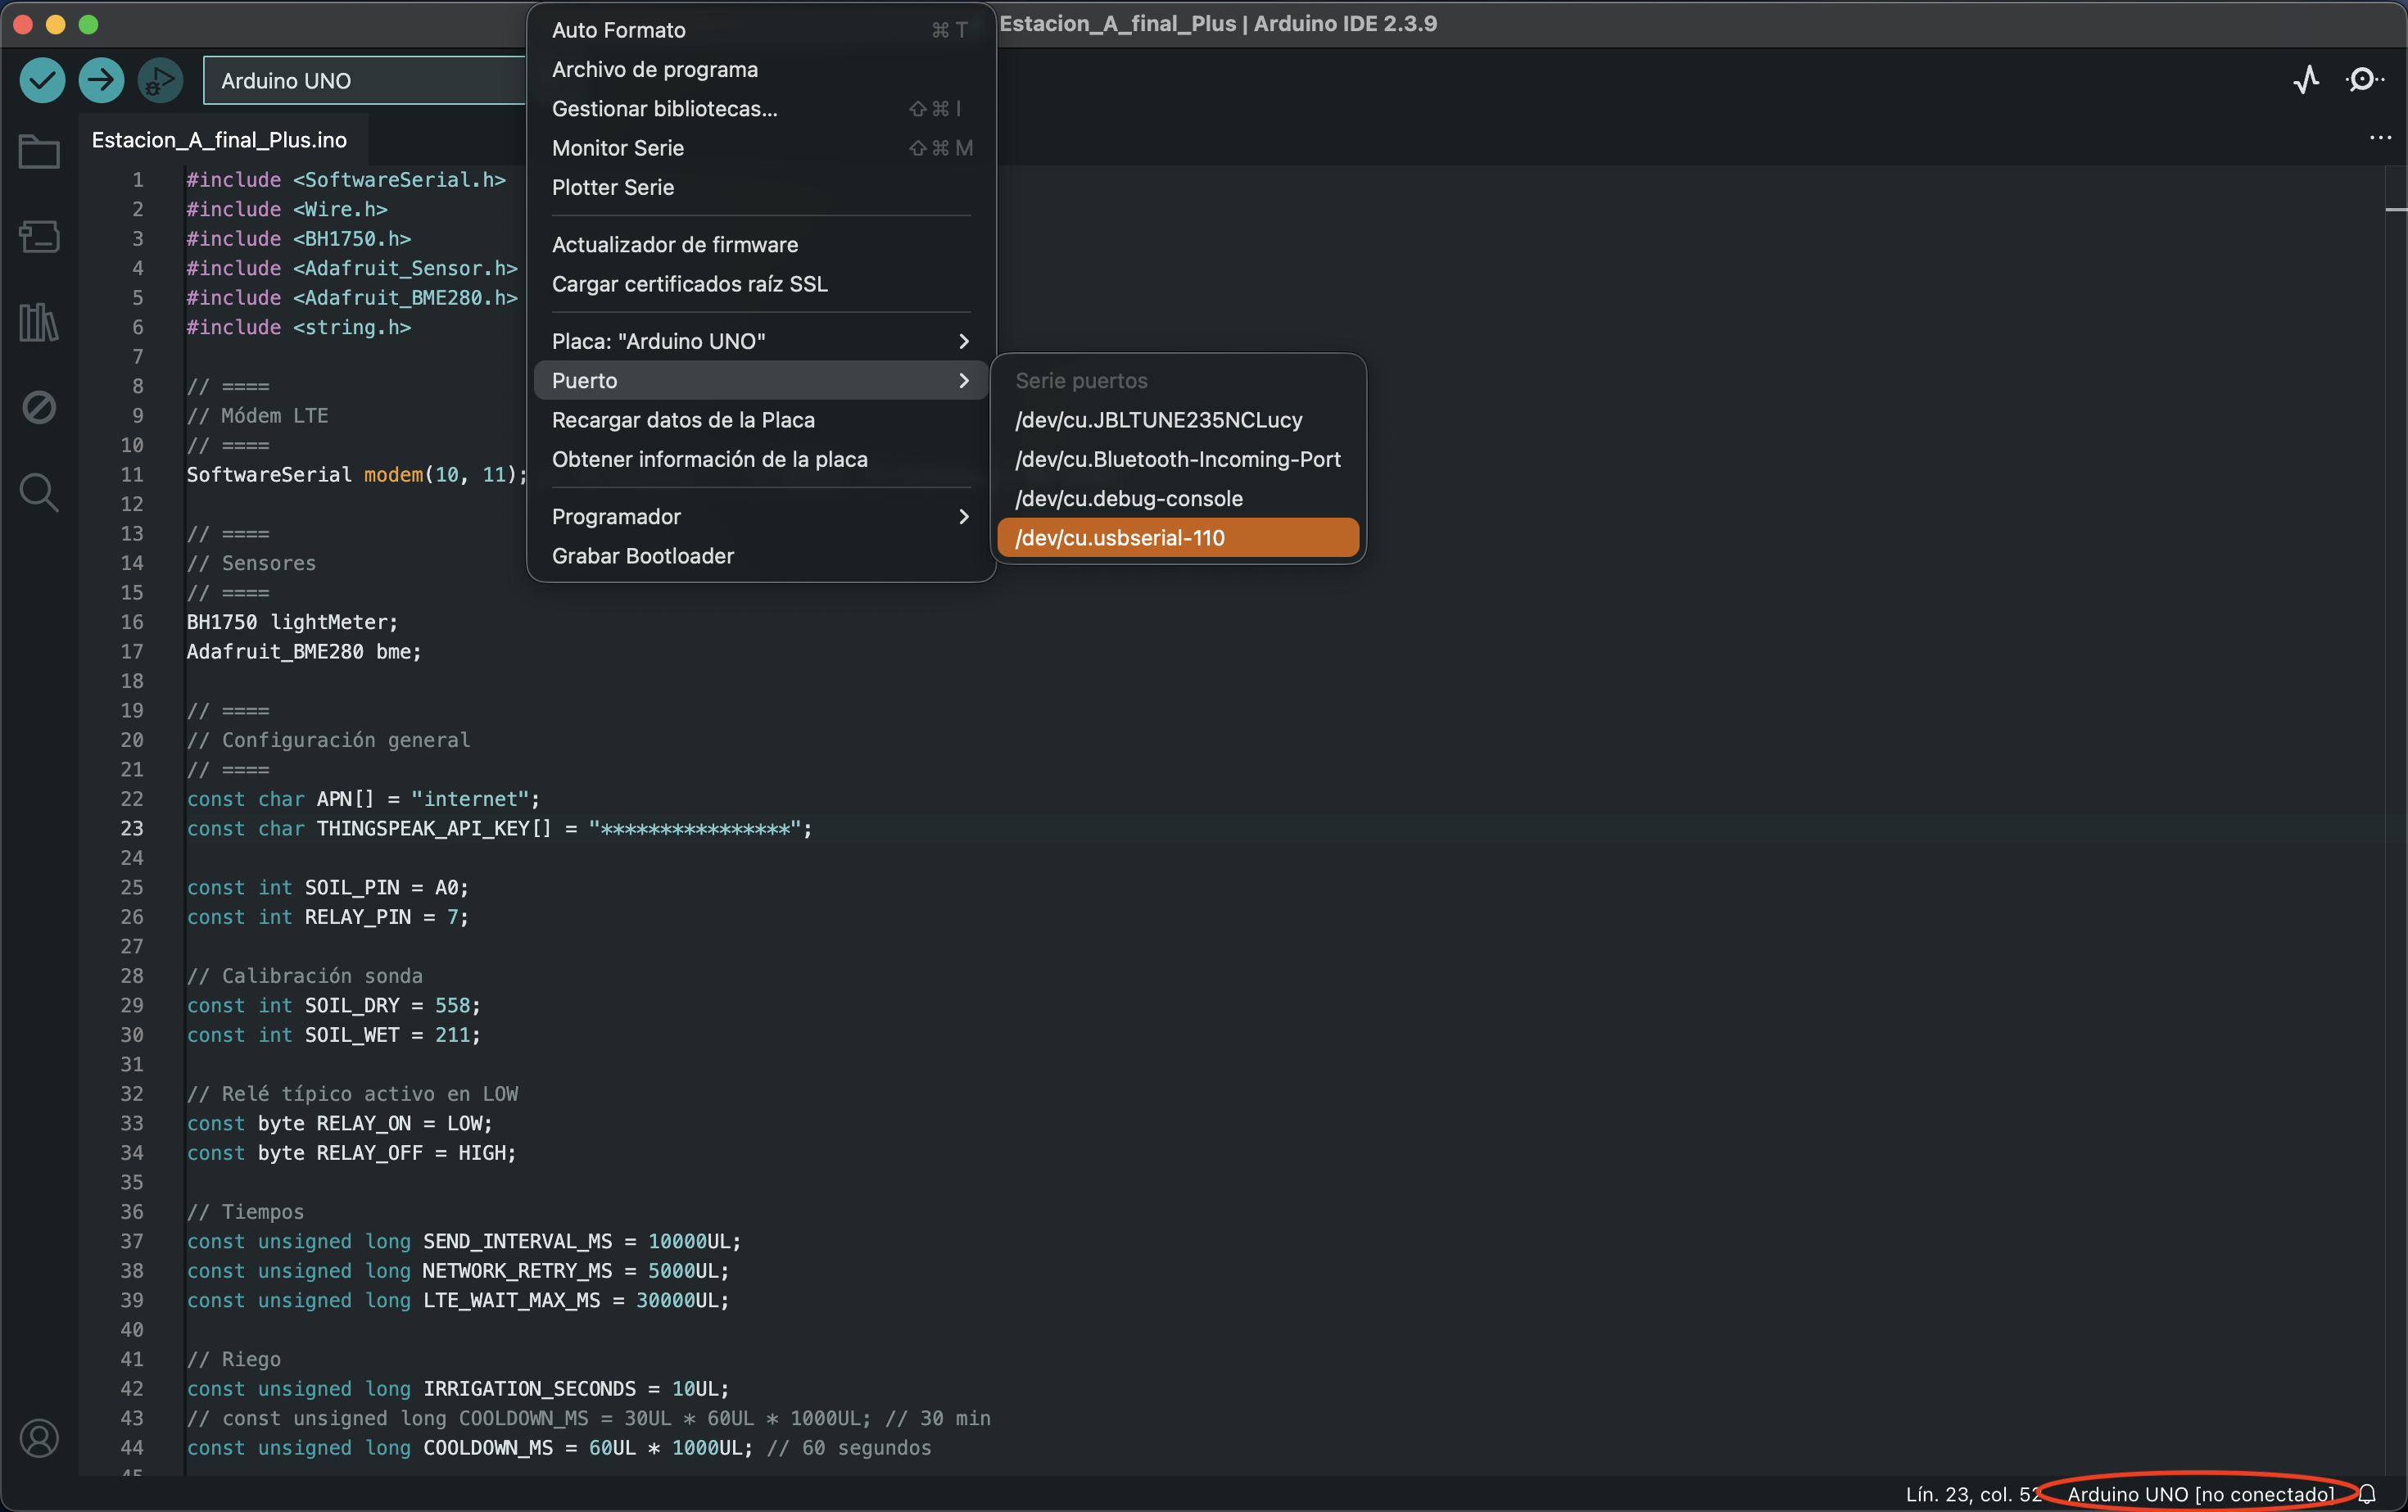
\includegraphics[width=0.92\textwidth]{figs/seleccion_puerto_Arduino.png}
    \caption{Selección del puerto serie correspondiente a la placa Arduino conectada por USB en Arduino IDE. Captura propia.}
    \label{fig:arduino_puerto_usb}
\end{figure}

Debe tenerse en cuenta que el nombre exacto del puerto serie puede variar según el sistema operativo, el adaptador USB empleado y el equipo utilizado durante la instalación.

\section{Instalación del software en Raspberry Pi}

En primer lugar se actualiza el sistema y se instalan las herramientas básicas:

\begin{bashcode}
sudo apt update
sudo apt upgrade -y
sudo apt install -y git python3 python3-venv python3-pip sqlite3
\end{bashcode}

Después se descarga el repositorio:

\begin{bashcode}
cd /home/pi
git clone https://github.com/ltejedorcruz/TierraViva.git
cd TierraViva
\end{bashcode}

Si el repositorio ya existe, puede actualizarse mediante:

\begin{bashcode}
cd /home/pi/TierraViva
git pull
\end{bashcode}

El repositorio incluye un fichero \texttt{requirements.txt} con las dependencias Python necesarias para ejecutar la API y el proceso de ingesta. Durante la instalación, el script \texttt{tierraviva.sh} crea un entorno virtual e instala automáticamente dichas dependencias mediante \texttt{pip}.

\section{Configuración del fichero \texttt{.env}}

El fichero \texttt{.env} debe crearse en la raíz del repositorio. Contiene la configuración local de estaciones, ThingSpeak y parámetros de ejecución.

\begin{bashcode}
nano .env
\end{bashcode}

Un ejemplo de configuración es:

\begin{bashcode}
STATIONS=A,B
STATION_ID=A

THINGSPEAK_CHANNEL_A=<CHANNEL_ID_A>
THINGSPEAK_READ_KEY_A=<READ_KEY_A>

THINGSPEAK_CHANNEL_B=<CHANNEL_ID_B>
THINGSPEAK_READ_KEY_B=<READ_KEY_B>

POLL_INTERVAL_SECONDS=10
REQUEST_TIMEOUT_SECONDS=12

TIERRAVIVA_LOG_LEVEL=INFO
\end{bashcode}

Para facilitar la reproducción del sistema, el repositorio incluye un fichero \texttt{.env.example} con la estructura de variables de entorno requerida. Este fichero no contiene claves reales ni identificadores privados, sino una plantilla que debe copiarse a \texttt{.env} y completarse con los canales y claves de lectura de ThingSpeak correspondientes.

\section{Preparación del \textit{dashboard}}

El \textit{dashboard} fuente se encuentra en el directorio:

\begin{terminaloutput}
dashboard/
\end{terminaloutput}

La interfaz principal se concentra en el fichero:

\begin{terminaloutput}
dashboard/index.html
\end{terminaloutput}

Este fichero incluye la estructura HTML, los estilos CSS embebidos y la lógica JavaScript necesaria para consultar la API y actualizar la interfaz. Los recursos gráficos se almacenan en:

\begin{terminaloutput}
dashboard/images/
\end{terminaloutput}

La API sirve la interfaz desde el directorio de ejecución:

\begin{terminaloutput}
frontend/
\end{terminaloutput}

Durante la instalación, el script \texttt{tierraviva.sh} sincroniza automáticamente el contenido de \texttt{dashboard/} con el directorio \texttt{frontend/}, que es el directorio servido por FastAPI. Esta copia incluye el fichero \texttt{index.html} y los recursos gráficos almacenados en \texttt{dashboard/images/}.

Si se desea realizar esta operación manualmente, o repetirla después de modificar el dashboard, puede ejecutarse:

\begin{bashcode}
mkdir -p frontend
cp -r dashboard/* frontend/
\end{bashcode}

Después de este paso debe existir, al menos:

\begin{terminaloutput}
frontend/index.html
frontend/images/
\end{terminaloutput}

La estructura actual concentra los estilos y la lógica JavaScript en el propio fichero \texttt{index.html}. Esta organización simplifica el despliegue del prototipo, reduce el número de rutas estáticas que deben sincronizarse durante las pruebas y facilita que FastAPI sirva la interfaz desde el directorio \texttt{frontend/}.

\section{Instalación mediante \textit{script}}

Antes de utilizar el \textit{script} debe concederse permiso de ejecución:

\begin{bashcode}
chmod +x tierraviva.sh
\end{bashcode}

La instalación inicial se realiza con:

\begin{bashcode}
./tierraviva.sh install
\end{bashcode}

Este comando prepara el entorno de ejecución del proyecto: crea el entorno virtual, instala dependencias, inicializa la base de datos y crea los directorios necesarios para la ejecución.

Tras la instalación, conviene comprobar que el dashboard se ha sincronizado correctamente con \texttt{frontend/}, especialmente el fichero \texttt{index.html} y el directorio \texttt{images/}:

\begin{bashcode}
ls frontend/
ls frontend/images
\end{bashcode}

La tabla \texttt{readings} almacena lecturas, \texttt{system\_state} conserva información de estado del sistema y \texttt{valve\_events} queda preparada para registrar eventos relacionados con la actuación.

\section{Arranque del sistema}

El sistema se arranca mediante:

\begin{bashcode}
./tierraviva.sh start
\end{bashcode}

Este comando inicia los procesos principales:

\begin{itemize}
    \item \texttt{main.py}, encargado de consultar ThingSpeak y almacenar lecturas nuevas;
    \item \texttt{api.py}, encargado de servir la API y el \textit{dashboard} web.
\end{itemize}

Para detener el sistema se utiliza:

\begin{bashcode}
./tierraviva.sh stop
\end{bashcode}

Para reiniciarlo:

\begin{bashcode}
./tierraviva.sh restart
\end{bashcode}

Para consultar el estado:

\begin{bashcode}
./tierraviva.sh status
\end{bashcode}

Para revisar los \textit{logs}:

\begin{bashcode}
./tierraviva.sh logs
\end{bashcode}

\section{Comprobación de la API}

Con el sistema arrancado, se comprueba primero el estado general de la API:

\begin{bashcode}
curl http://127.0.0.1:8000/api/health
\end{bashcode}

También puede comprobarse desde navegador:

\begin{terminaloutput}
http://<IP_RASPBERRY>:8000/api/health
\end{terminaloutput}

Otras comprobaciones útiles son:

\begin{terminaloutput}
http://<IP_RASPBERRY>:8000/api/config
http://<IP_RASPBERRY>:8000/api/latest?station=A
http://<IP_RASPBERRY>:8000/api/readings?station=A&limit=20
http://<IP_RASPBERRY>:8000/api/stats?station=A&hours=24
\end{terminaloutput}

La descripción completa de \textit{endpoints}, parámetros y respuestas se recoge en el Anexo~\ref{anexo:manual_api}.

\section{Acceso al \textit{dashboard}}

Una vez arrancada la API y copiado el \textit{dashboard} en \texttt{frontend/}, la interfaz web se abre desde:

\begin{terminaloutput}
http://<IP_RASPBERRY>:8000/
\end{terminaloutput}

Si se accede desde la propia Raspberry Pi, puede utilizarse:

\begin{terminaloutput}
http://127.0.0.1:8000/
\end{terminaloutput}

El \textit{dashboard} debe mostrar la estación seleccionada, la última lectura disponible, el estado de frescura, variables ambientales, estado de relé, eventos, gráficas y tabla de lecturas recientes.

\section{Comprobación extremo a extremo}

La instalación se considera preparada cuando se completa la siguiente secuencia:

\begin{table}[H]
\centering
\renewcommand{\arraystretch}{1.15}
\rowcolors{2}{TableRowSoft}{white}

\small
\begin{tabular}{|p{0.38\textwidth}|p{0.42\textwidth}|}
\hline
\rowcolor{URJCRed}
\TVHead{Comprobación} & \TVHead{Resultado esperado} \\
\hline
Estación encendida & Arduino, sensores y módem arrancan de forma estable.\\
\hline
Lectura de sensores & Valores coherentes en el monitor serie.\\
\hline
Registro LTE & El módem registra red móvil.\\
\hline
Publicación en ThingSpeak & Aparece una nueva entrada en el canal.\\
\hline
Ingesta en Raspberry Pi & \texttt{main.py} recupera una lectura nueva.\\
\hline
Inserción en SQLite & La lectura aparece en \texttt{readings}.\\
\hline
API operativa & \texttt{/api/health} responde correctamente.\\
\hline
\textit{Dashboard} visible & La interfaz muestra datos de la estación.\\
\hline
Prueba de relé aislada & El relé conmuta correctamente y vuelve a estado apagado.\\
\hline
Bomba temporizada & La bomba se activa y se apaga tras el tiempo configurado.\\
\hline
\end{tabular}
\caption{Checklist de comprobación extremo a extremo.}
\label{tab:checklist_extremo_a_extremo_instalacion}
\end{table}

\section{Problemas habituales}

\begin{table}[H]
\centering
\renewcommand{\arraystretch}{1.15}
\rowcolors{2}{TableRowSoft}{white}

\scriptsize
\begin{tabular}{|p{0.30\textwidth}|p{0.30\textwidth}|p{0.30\textwidth}|}
\hline
\rowcolor{URJCRed}
\TVHead{Problema} & \TVHead{Causa probable} & \TVHead{Acción recomendada} \\
\hline
Ausencia de datos en ThingSpeak & Clave de escritura incorrecta, APN incorrecto o fallo LTE. & Revisar \textit{firmware}, SIM, antena, APN y monitor serie. \\
\hline
Fallo de recuperación de datos en Raspberry Pi & Canal o clave de lectura incorrectos. & Revisar \texttt{THINGSPEAK\_CHANNEL\_A/B} y \texttt{THINGSPEAK\_READ\_KEY\_A/B}. \\
\hline
Fallo de arranque de la API & Entorno virtual o dependencias pendientes de preparar. & Ejecutar \texttt{./tierraviva.sh install}. \\
\hline
Fallo de carga del \textit{dashboard} & Ausencia de \texttt{frontend/index.html} o sincronización pendiente del contenido de \texttt{dashboard/}. & Ejecutar \texttt{./tierraviva.sh install} o, de forma manual, \texttt{cp -r dashboard/* frontend/}. Comprobar que existen \texttt{frontend/index.html} y \texttt{frontend/images/}. \\
\hline
El \textit{dashboard} carga con recursos gráficos ausentes & Sincronización incompleta del directorio \texttt{images/}. & Repetir \texttt{cp -r dashboard/* frontend/} y revisar que existen los ficheros gráficos en \texttt{frontend/images/}. \\
\hline
Ausencia de registros en SQLite & Publicación pendiente de la estación o ingestor inactivo. & Revisar ThingSpeak y \textit{logs} de \texttt{main.py}. \\
\hline
El relé se activa al arrancar & Lógica invertida o inicialización incorrecta. & Comprobar configuración del \textit{firmware} y probar sin bomba. \\
\hline
Bomba activa fuera del intervalo previsto & Error de cableado o uso del contacto incorrecto del relé. & Usar contacto normalmente abierto y validar apagado por \textit{firmware}. \\
\hline
El módulo LTE se reinicia & Alimentación insuficiente durante transmisión. & Revisar fuente, LM2596, corriente disponible y masa común. \\
\hline
\end{tabular}
\caption{Problemas habituales durante la instalación y puesta en marcha.}
\label{tab:problemas_instalacion_resumido}
\end{table}

\section{Conclusión}

La puesta en marcha de TierraViva debe realizarse por bloques: primero estación y sensores, después publicación en ThingSpeak, más tarde ingesta en Raspberry Pi, base de datos, API, \textit{dashboard} y finalmente actuación sobre relé o bomba. Esta secuencia permite aislar errores, localizar con mayor precisión fallos de montaje, configuración o comunicación, y comprobar cada capa antes de ejecutar una prueba completa.

\chapter{Manual de usuario de TierraViva}
\label{anexo:manual_usuario}

Este anexo describe el uso del sistema TierraViva desde el punto de vista del usuario final. A diferencia del manual de instalación, centrado en el despliegue técnico, este manual explica cómo acceder al \textit{dashboard}, cómo interpretar las lecturas, cómo comprobar el estado de las estaciones y cómo actuar ante situaciones habituales de funcionamiento.

\section{Alcance del manual}

Este manual cubre las operaciones de uso habituales:

\begin{itemize}
    \item acceso al \textit{dashboard} web;
    \item selección de estación;
    \item interpretación de lecturas actuales;
    \item interpretación del estado de humedad del suelo;
    \item revisión del estado de conexión;
    \item consulta de gráficas;
    \item revisión del resumen histórico;
    \item consulta de la tabla de últimas lecturas;
    \item interpretación de eventos y códigos de diagnóstico;
    \item comprobaciones básicas ante fallos.
\end{itemize}

No se incluyen en este manual las tareas de montaje eléctrico, instalación en Raspberry Pi o configuración de ThingSpeak, ya que dichas tareas se documentan en el Anexo \ref{anexo:manual_instalacion_sistema}. Tampoco se documentan en detalle los endpoints de la API, que se recogen en el Anexo \ref{anexo:manual_api}.

\section{Perfil de usuario}

El \textit{dashboard} de TierraViva puede ser utilizado por dos tipos principales de usuario:

\begin{table}[H]
\centering
\renewcommand{\arraystretch}{1.25}
\small
\begin{tabular}{|p{0.28\textwidth}|p{0.58\textwidth}|}
\hline
\rowcolor{gray!20}
\textbf{Perfil} & \textbf{Uso principal del sistema} \\
\hline
Usuario no técnico & Consultar el estado de la parcela, comprobar si el suelo está seco o húmedo y revisar si la estación está actualizando datos. \\
\hline
Usuario técnico & Verificar lecturas, revisar estado de conexión, comprobar eventos de sistema, analizar histórico y detectar posibles problemas de sensores, comunicación o \textit{backend}. \\
\hline
\end{tabular}
\caption{Perfiles de usuario previstos para TierraViva.}
\label{tab:perfiles_usuario_tierraviva}
\end{table}

\section{Acceso al \textit{dashboard}}

Una vez arrancado el sistema en la Raspberry Pi, el usuario accede al \textit{dashboard} desde un navegador web conectado a la misma red local.

\begin{verbatim}
http://<IP_RASPBERRY>:8000/
\end{verbatim}

Por ejemplo:

\begin{verbatim}
http://192.168.1.50:8000/
\end{verbatim}

La dirección exacta depende de la IP asignada a la Raspberry Pi en la red local. Si se accede desde la propia Raspberry Pi, también puede utilizarse:

\begin{verbatim}
http://127.0.0.1:8000/
\end{verbatim}

\section{Vista general del \textit{dashboard}}

El \textit{dashboard} está organizado en bloques visuales para que el estado del sistema pueda interpretarse rápidamente. La Tabla \ref{tab:zonas_dashboard} resume las zonas principales de la interfaz.

\begin{table}[H]
\centering
\renewcommand{\arraystretch}{1.25}
\small
\begin{tabular}{|p{0.30\textwidth}|p{0.55\textwidth}|}
\hline
\rowcolor{gray!20}
\textbf{Zona del dashboard} & \textbf{Información mostrada} \\
\hline
Cabecera & Nombre del sistema, estado de conexión y selector de estación. \\
\hline
Tarjetas de lectura actual & Humedad del suelo, temperatura, humedad ambiental, luminosidad y presión. \\
\hline
Estado de última lectura & Frescura del dato, hora de actualización y estado general. \\
\hline
Estado/evento & Código o evento de funcionamiento recibido desde la estación. \\
\hline
Debug/código & Código auxiliar de diagnóstico. \\
\hline
Gráficas & Evolución reciente de las variables almacenadas. \\
\hline
Resumen histórico & Estadísticas de las últimas 24 horas. \\
\hline
Tabla de últimas lecturas & Registros recientes almacenados en SQLite. \\
\hline
\end{tabular}
\caption{Zonas principales del \textit{dashboard} TierraViva.}
\label{tab:zonas_dashboard}
\end{table}

\section{Selección de estación}

Si el sistema tiene más de una estación configurada, el \textit{dashboard} permite seleccionar la estación activa mediante un desplegable. En la configuración actual están disponibleslas estaciones \texttt{A} y \texttt{B}.

Al seleccionar una estación, el \textit{dashboard} actualiza:

\begin{itemize}
    \item lectura actual;
    \item estado de humedad;
    \item gráficas;
    \item resumen histórico;
    \item tabla de últimas lecturas;
    \item códigos de evento y diagnóstico.
\end{itemize}

Esta separación evita mezclar datos de distintas estaciones y permite comparar zonas diferentes de una parcela o distintos entornos de prueba.

\section{Interpretación de lecturas actuales}

Las tarjetas principales muestran la última lectura disponible para la estación seleccionada.

\begin{table}[H]
\centering
\renewcommand{\arraystretch}{1.25}
\small
\begin{tabular}{|p{0.26\textwidth}|p{0.22\textwidth}|p{0.38\textwidth}|}
\hline
\rowcolor{gray!20}
\textbf{Variable} & \textbf{Unidad} & \textbf{Interpretación} \\
\hline
Humedad del suelo & \% & Variable principal para evaluar si el sustrato está seco, normal o húmedo. \\
\hline
Temperatura & $^\circ$C & Temperatura ambiente medida por la estación. \\
\hline
Humedad ambiental & \% & Humedad relativa del aire. \\
\hline
Luminosidad & lux & Intensidad luminosa recibida por el sensor BH1750. \\
\hline
Presión & hPa & Presión atmosférica medida por el sensor BME280. \\
\hline
\end{tabular}
\caption{Lecturas actuales mostradas por el \textit{dashboard}.}
\label{tab:lecturas_actuales_dashboard}
\end{table}

Si una variable aparece como ``---'', significa que no existe dato disponible para esa lectura, que el sensor no ha enviado valor o que todavía no se ha almacenado ninguna lectura válida.

\section{Estado de humedad del suelo}

El \textit{dashboard} clasifica la humedad del suelo en tres estados: seco, normal y húmedo. Esta clasificación se calcula utilizando los umbrales configurados en la API.

\begin{table}[H]
\centering
\renewcommand{\arraystretch}{1.25}
\small
\begin{tabular}{|p{0.24\textwidth}|p{0.28\textwidth}|p{0.34\textwidth}|}
\hline
\rowcolor{gray!20}
\textbf{Estado} & \textbf{Condición} & \textbf{Interpretación} \\
\hline
Seco & Humedad inferior al umbral bajo & El sustrato puede requerir riego según la lógica configurada en la estación. \\
\hline
Normal & Humedad entre umbral bajo y alto & El suelo se encuentra en una zona intermedia. \\
\hline
Húmedo & Humedad superior al umbral alto & El suelo dispone de humedad suficiente. \\
\hline
Sin dato & No hay lectura válida & No se debe interpretar el estado hídrico hasta recibir una lectura correcta. \\
\hline
\end{tabular}
\caption{Interpretación del estado de humedad del suelo.}
\label{tab:estado_humedad_suelo}
\end{table}

En la configuración por defecto, los umbrales utilizados por el \textit{dashboard} son 35\% para el límite bajo y 45\% para el límite alto. Estos valores pueden modificarse en el fichero de configuración \texttt{.env} mediante las variables \texttt{SOIL\_LOW\_THRESHOLD} y \texttt{SOIL\_HIGH\_THRESHOLD}.

\section{Estado de conexión y frescura de datos}

El \textit{dashboard} no solo muestra la última lectura, sino también su antigüedad. Esto permite saber si la estación está actualizando datos de forma reciente o si se ha perdido continuidad en la telemetría.

\begin{table}[H]
\centering
\renewcommand{\arraystretch}{1.25}
\small
\begin{tabular}{|p{0.24\textwidth}|p{0.30\textwidth}|p{0.32\textwidth}|}
\hline
\rowcolor{gray!20}
\textbf{Estado} & \textbf{Condición} & \textbf{Interpretación} \\
\hline
En vivo & Lectura reciente & La estación está enviando datos y la Raspberry Pi los está actualizando correctamente. \\
\hline
Datos recientes & Lectura algo antigua, pero dentro del margen permitido & El sistema tiene datos válidos, aunque conviene vigilar si continúa actualizando. \\
\hline
Sin actualización & Lectura antigua & Puede existir un problema de comunicación, publicación, ingesta o alimentación. \\
\hline
Sin datos & No existe ninguna lectura almacenada & La estación no ha publicado todavía o la Raspberry Pi no ha podido recuperar datos. \\
\hline
\end{tabular}
\caption{Estados de conexión y frescura de datos.}
\label{tab:estado_conexion_dashboard}
\end{table}

El tiempo utilizado para clasificar una lectura como reciente o antigua se controla mediante la variable \texttt{DATA\_STALE\_SECONDS}. En la configuración por defecto se utiliza un valor de 90 segundos.

\section{Estado del relé}

El \textit{dashboard} muestra el estado del relé recibido desde la estación. Este valor procede de la telemetría publicada en ThingSpeak y permite saber si el sistema de actuación está apagado o activo en el momento de la lectura.

\begin{table}[H]
\centering
\renewcommand{\arraystretch}{1.25}
\small
\begin{tabular}{|p{0.20\textwidth}|p{0.28\textwidth}|p{0.38\textwidth}|}
\hline
\rowcolor{gray!20}
\textbf{Valor} & \textbf{Estado mostrado} & \textbf{Interpretación} \\
\hline
0 & OFF & El relé está apagado y la bomba no debería estar activa. \\
\hline
1 & Activo & El relé está activo y el sistema de riego puede estar funcionando. \\
\hline
Sin dato & Sin dato & No se ha recibido información válida del relé. \\
\hline
\end{tabular}
\caption{Interpretación del estado del relé.}
\label{tab:estado_rele_dashboard}
\end{table}

El usuario debe tener en cuenta que el \textit{dashboard} muestra el estado recibido en la última lectura almacenada. Si existe retraso de comunicación, el estado físico real puede haber cambiado antes de que el \textit{dashboard} se actualice.

\section{Eventos de sistema}

El campo de evento permite interpretar el estado interno de la estación. La Tabla \ref{tab:eventos_sistema_usuario} recoge los códigos utilizados por el \textit{dashboard}.

\begin{table}[H]
\centering
\renewcommand{\arraystretch}{1.25}
\small
\begin{tabular}{|c|p{0.28\textwidth}|p{0.42\textwidth}|}
\hline
\rowcolor{gray!20}
\textbf{Código} & \textbf{Evento} & \textbf{Interpretación} \\
\hline
100 & \texttt{idle} & Estación en reposo, sin riego activo. \\
\hline
206 & \texttt{safe mode} & La estación trabaja en modo seguro. \\
\hline
210 & \texttt{riego ON} & La estación ha activado el riego. \\
\hline
211 & \texttt{riego OFF} & La estación ha finalizado el riego. \\
\hline
400 & \texttt{error} & Existe un fallo relevante o una lectura no válida. \\
\hline
429 & \texttt{cooldown} & El riego está bloqueado temporalmente por periodo de seguridad. \\
\hline
\end{tabular}
\caption{Eventos de sistema mostrados en el \textit{dashboard}.}
\label{tab:eventos_sistema_usuario}
\end{table}

Estos códigos ayudan a diferenciar una situación normal de reposo de un bloqueo por seguridad o de un error real del sistema.

\section{Códigos de diagnóstico}

El campo de diagnóstico aporta información auxiliar sobre el estado del ciclo de funcionamiento de la estación.

\begin{table}[H]
\centering
\renewcommand{\arraystretch}{1.25}
\small
\begin{tabular}{|c|p{0.28\textwidth}|p{0.42\textwidth}|}
\hline
\rowcolor{gray!20}
\textbf{Código} & \textbf{Etiqueta} & \textbf{Interpretación} \\
\hline
200 & OK & Funcionamiento correcto. \\
\hline
204 & no riego & No se ha activado el riego en el ciclo actual. \\
\hline
206 & modo seguro & La estación se encuentra en modo seguro. \\
\hline
400 & error & Se ha detectado un error. \\
\hline
429 & \textit{cooldown} & La estación evita un nuevo riego por seguridad temporal. \\
\hline
\end{tabular}
\caption{Códigos de diagnóstico mostrados en el \textit{dashboard}.}
\label{tab:codigos_diagnostico_usuario}
\end{table}

\section{Gráficas}

El \textit{dashboard} incluye gráficas de evolución reciente para las variables almacenadas. Estas gráficas permiten detectar tendencias de forma rápida, por ejemplo:

\begin{itemize}
    \item descenso progresivo de humedad del suelo;
    \item aumento de temperatura durante el día;
    \item variación de luminosidad;
    \item cambios de humedad ambiental;
    \item activaciones puntuales del relé;
    \item repetición de eventos de error o \textit{cooldown}.
\end{itemize}

Las gráficas se construyen a partir de las últimas lecturas almacenadas en SQLite. Si no existen datos suficientes, la gráfica mostrará un mensaje indicando que todavía no hay información disponible.

\section{Resumen histórico}

El resumen histórico muestra estadísticas de las últimas 24 horas para la estación seleccionada. Incluye número de muestras, fecha inicial y final de la ventana temporal, valores medios, mínimos y máximos.

\begin{table}[H]
\centering
\renewcommand{\arraystretch}{1.25}
\small
\begin{tabular}{|p{0.30\textwidth}|p{0.55\textwidth}|}
\hline
\rowcolor{gray!20}
\textbf{Dato histórico} & \textbf{Utilidad} \\
\hline
Número de muestras & Permite comprobar si la estación está enviando datos con regularidad. \\
\hline
Valor medio & Resume el comportamiento de una variable durante la ventana analizada. \\
\hline
Valor mínimo & Ayuda a detectar extremos, por ejemplo humedad mínima del suelo. \\
\hline
Valor máximo & Ayuda a detectar picos de temperatura, luminosidad o presión. \\
\hline
Primer y último registro & Permiten comprobar el intervalo real cubierto por los datos. \\
\hline
\end{tabular}
\caption{Interpretación del resumen histórico.}
\label{tab:resumen_historico_usuario}
\end{table}

\section{Tabla de últimas lecturas}

La tabla de últimas lecturas muestra registros recientes almacenados en la base de datos local. Cada fila corresponde a una lectura recuperada desde ThingSpeak y guardada por la Raspberry Pi.

La tabla permite revisar:

\begin{itemize}
    \item fecha y hora de cada lectura;
    \item humedad del suelo;
    \item temperatura;
    \item humedad ambiental;
    \item luminosidad;
    \item presión atmosférica.
\end{itemize}

Esta vista es útil para verificar si los datos evolucionan de forma coherente o si aparecen valores repetidos, ausentes o fuera de rango.

\section{Procedimiento de uso diario}

Una vez instalado el sistema, el uso habitual puede resumirse en los siguientes pasos:

\begin{enumerate}
    \item encender la estación remota y comprobar que queda alimentada correctamente;
    \item arrancar el sistema en Raspberry Pi mediante \texttt{./tierraviva.sh start};
    \item abrir el \textit{dashboard} desde un navegador;
    \item seleccionar la estación que se desea consultar;
    \item comprobar el estado de conexión;
    \item revisar la humedad del suelo;
    \item interpretar el estado del relé y los códigos de evento;
    \item consultar las gráficas si se desea analizar evolución;
    \item revisar la tabla de últimas lecturas ante cualquier valor anómalo;
    \item detener el sistema con \texttt{Ctrl+C} o mediante el comando de parada correspondiente si se está ejecutando como proceso gestionado.
\end{enumerate}

\section{Situaciones habituales y actuación recomendada}

\begin{table}[H]
\centering
\renewcommand{\arraystretch}{1.25}
\scriptsize
\begin{tabular}{|p{0.28\textwidth}|p{0.32\textwidth}|p{0.30\textwidth}|}
\hline
\rowcolor{gray!20}
\textbf{Situación observada} & \textbf{Interpretación probable} & \textbf{Actuación recomendada} \\
\hline
El \textit{dashboard} muestra ``Sin datos'' & No hay lecturas almacenadas para la estación seleccionada. & Comprobar que la estación publica en ThingSpeak y que \texttt{main.py} está ejecutándose. \\
\hline
El estado aparece como ``Sin actualización'' & La última lectura es demasiado antigua. & Revisar alimentación de la estación, cobertura LTE, canal ThingSpeak y \textit{logs} de Raspberry Pi. \\
\hline
La humedad aparece como ``Seco'' & El valor está por debajo del umbral bajo. & Verificar si la estación ejecuta riego local o si se mantiene bloqueada por \textit{cooldown}. \\
\hline
Aparece código 429 & La estación está en periodo de seguridad entre riegos. & Esperar a que finalice el \textit{cooldown} y revisar si el valor de humedad sigue siendo bajo. \\
\hline
Aparece código 400 & Se ha detectado un error o lectura no válida. & Revisar sensores, cableado, alimentación y monitor serie de la estación. \\
\hline
El relé aparece activo & La última telemetría indica relé encendido. & Comprobar físicamente si la bomba está funcionando y verificar que se apaga al finalizar el tiempo programado. \\
\hline
Las gráficas no muestran datos & No hay histórico suficiente o la API no devuelve lecturas. & Esperar nuevas lecturas y comprobar \texttt{/api/readings}. \\
\hline
Los valores no cambian durante mucho tiempo & Puede no haber nuevas publicaciones o el ingestor está ignorando duplicados. & Revisar entry\_id en ThingSpeak, \textit{logs} de \texttt{main.py} y estado de la estación. \\
\hline
\end{tabular}
\caption{Situaciones habituales durante el uso de TierraViva.}
\label{tab:situaciones_usuario_tierraviva}
\end{table}

\section{Buenas prácticas de uso}

Para utilizar TierraViva de forma segura y fiable se recomienda:

\begin{itemize}
    \item verificar que la estación arranca con el relé apagado;
    \item no dejar la bomba conectada durante pruebas iniciales sin supervisión;
    \item revisar periódicamente el estado de conexión del \textit{dashboard};
    \item comprobar que la humedad del suelo cambia de forma coherente;
    \item no modificar umbrales sin registrar el cambio;
    \item no compartir capturas que contengan claves API;
    \item mantener la electrónica protegida frente a agua y salpicaduras;
    \item revisar \textit{logs} si aparecen estados de error o datos obsoletos;
    \item contrastar el \textit{dashboard} con una observación física durante pruebas de riego.
\end{itemize}

\section{Conclusión}

El \textit{dashboard} de TierraViva permite supervisar de forma sencilla el estado de una o varias estaciones de riego inteligente. La interfaz resume las variables principales, clasifica el estado de humedad, muestra la frescura de los datos, representa gráficas recientes y permite revisar histórico almacenado en la Raspberry Pi.

El usuario debe interpretar el sistema como una herramienta de monitorización y apoyo a la validación del prototipo. La actuación sobre el riego se realiza en la estación Arduino mediante lógica local, mientras que el \textit{dashboard} permite comprobar si las lecturas, eventos y estados publicados son coherentes con el funcionamiento esperado.
\chapter{Manual de referencia de la API}
\label{anexo:manual_api}

Este anexo documenta la API local de TierraViva implementada sobre FastAPI. Su finalidad es servir como referencia técnica para consultar los \textit{endpoints} disponibles, sus parámetros, las respuestas esperadas y los errores más habituales.

La API se ejecuta en la Raspberry Pi y trabaja sobre los datos almacenados previamente en SQLite. No consulta directamente los sensores ni se comunica por puerto serie con las estaciones. Las lecturas son publicadas por las estaciones en ThingSpeak, recuperadas por el ingestor \texttt{main.py}, almacenadas mediante \texttt{database.py} y expuestas posteriormente por \texttt{api.py}.

\section{Alcance}

La versión actual de la API permite:

\begin{itemize}
    \item servir el \textit{dashboard} web desde la ruta raíz;
    \item consultar la configuración activa del sistema;
    \item obtener la última lectura de una estación;
    \item recuperar lecturas históricas recientes;
    \item calcular estadísticas por estación y ventana temporal;
    \item comprobar el estado básico del servicio.
\end{itemize}

\section{URL base}

Durante el despliegue local en Raspberry Pi, la API se sirve en el puerto \texttt{8000}. Desde la propia Raspberry Pi puede consultarse mediante:

\begin{verbatim}
http://127.0.0.1:8000
\end{verbatim}

Desde otro equipo conectado a la misma red local:

\begin{verbatim}
http://<IP_RASPBERRY>:8000
\end{verbatim}

\section{Convenciones generales}

Todas las respuestas de la API se devuelven en formato JSON, salvo la ruta raíz \texttt{/}, que sirve el fichero HTML del \textit{dashboard}.

En las respuestas JSON se utiliza habitualmente el campo \texttt{ok}:

\begin{itemize}
    \item \texttt{ok: true}: la petición se ha procesado correctamente;
    \item \texttt{ok: false}: la petición es válida, pero no existen datos para devolver.
\end{itemize}

El parámetro de estación se denomina \texttt{station}. Si se omite, la API utiliza la estación configurada por defecto mediante la variable \texttt{STATION\_ID}.

\section{Variables de configuración utilizadas}

La Tabla~\ref{tab:variables_api_resumidas} recoge las variables de entorno que afectan directamente al comportamiento de la API.

\begin{table}[H]
\centering
\renewcommand{\arraystretch}{1.15}
\rowcolors{2}{TableRowSoft}{white}
\small
\begin{tabular}{|p{0.32\textwidth}|p{0.18\textwidth}|p{0.38\textwidth}|}
\hline
\rowcolor{URJCRed}
\TVHead{Variable} & \TVHead{Valor por defecto} & \TVHead{Uso} \\
\hline
\texttt{TIERRAVIVA\_HOME} & \texttt{\textasciitilde/tierraviva} & Ruta base usada para localizar \texttt{data/}, \texttt{frontend/} y la base SQLite. \\
\hline
\texttt{STATION\_ID} & \texttt{A} & Estación seleccionada por defecto. \\
\hline
\texttt{STATIONS} & \texttt{A,B} & Lista de estaciones activas mostradas por la API. \\
\hline
\texttt{SOIL\_LOW\_THRESHOLD} & \texttt{35} & Umbral inferior para clasificar humedad del suelo. \\
\hline
\texttt{SOIL\_HIGH\_THRESHOLD} & \texttt{45} & Umbral superior para clasificar humedad del suelo. \\
\hline
\texttt{WEB\_REFRESH\_SECONDS} & \texttt{3} & Intervalo de refresco recomendado para el \textit{dashboard}. \\
\hline
\texttt{DATA\_STALE\_SECONDS} & \texttt{90} & Tiempo utilizado para clasificar una lectura como reciente, antigua u \textit{offline}. \\
\hline
\end{tabular}
\caption{Variables de configuración utilizadas por la API.}
\label{tab:variables_api_resumidas}
\end{table}

Las variables de ThingSpeak no se utilizan directamente en \texttt{api.py}; se emplean en el proceso de ingesta \texttt{main.py}.

\section{Resumen de \textit{endpoints}}

\begin{table}[H]
\centering
\renewcommand{\arraystretch}{1.25}
\small
\begin{tabular}{|p{0.16\textwidth}|p{0.28\textwidth}|p{0.42\textwidth}|}
\hline
\rowcolor{URJCRed}
\TVHead{Método} & \TVHead{Endpoint} & \TVHead{Función} \\
\hline
GET & \texttt{/} & Sirve el \textit{dashboard} web desde \texttt{frontend/index.html}. \\
\hline
GET & \texttt{/api/config} & Devuelve configuración activa y estado básico de ingesta. \\
\hline
GET & \texttt{/api/latest} & Devuelve la última lectura almacenada de una estación. \\
\hline
GET & \texttt{/api/readings} & Devuelve el histórico reciente de lecturas de una estación. \\
\hline
GET & \texttt{/api/stats} & Devuelve estadísticas agregadas de una estación. \\
\hline
GET & \texttt{/api/health} & Comprueba el estado básico de API, base de datos y \textit{frontend}. \\
\hline
\end{tabular}
\caption{\textit{Endpoints} disponibles en la API actual de TierraViva.}
\label{tab:endpoints_api_actual}
\end{table}

\section{GET /}

Sirve la interfaz web principal del \textit{dashboard}.

\subsection*{Petición}

\begin{verbatim}
GET http://<IP_RASPBERRY>:8000/
\end{verbatim}

\subsection*{Respuesta esperada}

Si el fichero \texttt{frontend/index.html} existe, el navegador muestra el \textit{dashboard} de TierraViva.

\subsection*{Error posible}

Si el fichero no existe, la API devuelve un error HTTP 404:

\begin{verbatim}
{
  "detail": "No se encontró frontend/index.html"
}
\end{verbatim}

\section{GET /api/config}

Devuelve la configuración activa de la API para una estación.

\subsection*{Parámetros}

\begin{table}[H]
\centering
\renewcommand{\arraystretch}{1.25}
\small
\begin{tabular}{|p{0.20\textwidth}|p{0.18\textwidth}|p{0.18\textwidth}|p{0.30\textwidth}|}
\hline
\rowcolor{URJCRed}
\TVHead{Parámetro} & \TVHead{Tipo} & \TVHead{Obligatorio} & \TVHead{Descripción} \\
\hline
\texttt{station} & texto & No & Estación consultada. Si se omite, se utiliza \texttt{STATION\_ID}. \\
\hline
\end{tabular}
\caption{Parámetros de \texttt{/api/config}.}
\label{tab:parametros_api_config_resumido}
\end{table}

\subsection*{Ejemplo}

\begin{verbatim}
curl "http://127.0.0.1:8000/api/config?station=A"
\end{verbatim}

\subsection*{Respuesta esperada}

\begin{verbatim}
{
  "ok": true,
  "station_id": "A",
  "active_stations": ["A", "B"],
  "soil_low_threshold": 35.0,
  "soil_high_threshold": 45.0,
  "web_refresh_seconds": 3,
  "data_stale_seconds": 90,
  "base_dir": "/home/pi/TierraViva",
  "database_path": "/home/pi/TierraViva/data/tierraviva.db",
  "last_ingest_ts": "2026-06-01T10:15:00Z",
  "last_entry_id": "125"
}
\end{verbatim}

\section{GET /api/latest}

Devuelve la última lectura almacenada para una estación.

\subsection*{Parámetros}

\begin{table}[H]
\centering
\renewcommand{\arraystretch}{1.25}
\small
\begin{tabular}{|p{0.20\textwidth}|p{0.18\textwidth}|p{0.18\textwidth}|p{0.30\textwidth}|}
\hline
\rowcolor{URJCRed}
\TVHead{Parámetro} & \TVHead{Tipo} & \TVHead{Obligatorio} & \TVHead{Descripción} \\
\hline
\texttt{station} & texto & No & Estación consultada, por ejemplo \texttt{A} o \texttt{B}. \\
\hline
\end{tabular}
\caption{Parámetros de \texttt{/api/latest}.}
\label{tab:parametros_api_latest_resumido}
\end{table}

\subsection*{Ejemplo}

\begin{verbatim}
curl "http://127.0.0.1:8000/api/latest?station=A"
\end{verbatim}

\subsection*{Respuesta con datos}

\begin{verbatim}
{
  "ok": true,
  "station_id": "A",
  "reading": {
    "id": 32,
    "entry_id": 125,
    "station_id": "A",
    "ts": "2026-06-01T10:15:00Z",
    "soil_moisture_pct": 38.5,
    "temperature_c": 24.1,
    "humidity_pct": 52.0,
    "light_lux": 760.0,
    "pressure_hpa": 1012.4,
    "relay_state": 0,
    "system_event": 100,
    "debug_code": 204,
    "source": "thingspeak",
    "raw_json": "{...}"
  },
  "age_seconds": 8,
  "freshness": "fresh",
  "soil_state": "normal"
}
\end{verbatim}

\subsection*{Respuesta sin datos}

\begin{verbatim}
{
  "ok": false,
  "station_id": "A",
  "reading": null,
  "status": "sin_datos"
}
\end{verbatim}

\section{GET /api/readings}

Devuelve una lista de lecturas recientes almacenadas para una estación.

\subsection*{Parámetros}

\begin{table}[H]
\centering
\renewcommand{\arraystretch}{1.25}
\small
\begin{tabular}{|p{0.20\textwidth}|p{0.18\textwidth}|p{0.18\textwidth}|p{0.30\textwidth}|}
\hline
\rowcolor{URJCRed}
\TVHead{Parámetro} & \TVHead{Tipo} & \TVHead{Obligatorio} & \TVHead{Descripción} \\
\hline
\texttt{station} & texto & No & Estación consultada. \\
\hline
\texttt{limit} & entero & No & Número máximo de lecturas devueltas. Rango permitido: 1 a 500. Valor por defecto: 120. \\
\hline
\end{tabular}
\caption{Parámetros de \texttt{/api/readings}.}
\label{tab:parametros_api_readings_resumido}
\end{table}

\subsection*{Ejemplo}

\begin{verbatim}
curl "http://127.0.0.1:8000/api/readings?station=A&limit=20"
\end{verbatim}

\subsection*{Respuesta esperada}

\begin{verbatim}
{
  "ok": true,
  "station_id": "A",
  "count": 20,
  "readings": [
    {
      "id": 32,
      "entry_id": 125,
      "station_id": "A",
      "ts": "2026-06-01T10:15:00Z",
      "soil_moisture_pct": 38.5,
      "temperature_c": 24.1,
      "humidity_pct": 52.0,
      "light_lux": 760.0,
      "pressure_hpa": 1012.4,
      "relay_state": 0,
      "system_event": 100,
      "debug_code": 204,
      "source": "thingspeak",
      "raw_json": "{...}"
    }
  ]
}
\end{verbatim}

\section{GET /api/stats}

Devuelve estadísticas agregadas de una estación durante una ventana temporal.

\subsection*{Parámetros}

\begin{table}[H]
\centering
\renewcommand{\arraystretch}{1.25}
\small
\begin{tabular}{|p{0.20\textwidth}|p{0.18\textwidth}|p{0.18\textwidth}|p{0.30\textwidth}|}
\hline
\rowcolor{URJCRed}
\TVHead{Parámetro} & \TVHead{Tipo} & \TVHead{Obligatorio} & \TVHead{Descripción} \\
\hline
\texttt{station} & texto & No & Estación consultada. \\
\hline
\texttt{hours} & entero & No & Ventana temporal en horas. Rango permitido: 1 a 720. Valor por defecto: 24. \\
\hline
\end{tabular}
\caption{Parámetros de \texttt{/api/stats}.}
\label{tab:parametros_api_stats_resumido}
\end{table}

\subsection*{Ejemplo}

\begin{verbatim}
curl "http://127.0.0.1:8000/api/stats?station=A&hours=24"
\end{verbatim}

\subsection*{Respuesta esperada}

La respuesta incluye el identificador de estación, la ventana temporal, el número de muestras y estadísticas agregadas de las variables medidas.

\begin{verbatim}
{
  "ok": true,
  "station_id": "A",
  "hours": 24,
  "samples": 18,
  "window_start": "2026-06-01T00:00:00Z",
  "first_ts": "2026-06-01T08:30:00Z",
  "last_ts": "2026-06-01T10:15:00Z",
  "soil": {
    "avg": 39.2,
    "min": 35.8,
    "max": 44.1
  },
  "temperature": {
    "avg": 24.0,
    "min": 21.8,
    "max": 26.5
  },
  "humidity": {
    "avg": 53.1,
    "min": 48.0,
    "max": 60.2
  },
  "light": {
    "avg": 650.5,
    "min": 120.0,
    "max": 980.0
  },
  "pressure": {
    "avg": 1012.3,
    "min": 1010.8,
    "max": 1013.6
  }
}
\end{verbatim}

\section{GET /api/health}

Devuelve una comprobación básica del estado del servicio.

\subsection*{Parámetros}

\begin{table}[H]
\centering
\renewcommand{\arraystretch}{1.25}
\small
\begin{tabular}{|p{0.20\textwidth}|p{0.18\textwidth}|p{0.18\textwidth}|p{0.30\textwidth}|}
\hline
\rowcolor{URJCRed}
\TVHead{Parámetro} & \TVHead{Tipo} & \TVHead{Obligatorio} & \TVHead{Descripción} \\
\hline
\texttt{station} & texto & No & Estación sobre la que se comprueba si existen datos. \\
\hline
\end{tabular}
\caption{Parámetros de \texttt{/api/health}.}
\label{tab:parametros_api_health_resumido}
\end{table}

\subsection*{Ejemplo}

\begin{verbatim}
curl "http://127.0.0.1:8000/api/health?station=A"
\end{verbatim}

\subsection*{Respuesta esperada}

\begin{verbatim}
{
  "ok": true,
  "station_id": "A",
  "active_stations": ["A", "B"],
  "database": "/home/pi/TierraViva/data/tierraviva.db",
  "frontend_exists": true,
  "has_data": true
}
\end{verbatim}

\section{Campos principales de una lectura}

Las lecturas devueltas por la API proceden de la tabla \texttt{readings}. La Tabla~\ref{tab:campos_lectura_api_resumido} resume los campos más relevantes para el consumo desde el \textit{dashboard}.

\begin{table}[H]
\centering
\renewcommand{\arraystretch}{1.25}
\scriptsize
\begin{tabular}{|p{0.30\textwidth}|p{0.18\textwidth}|p{0.40\textwidth}|}
\hline
\rowcolor{URJCRed}
\TVHead{Campo} & \TVHead{Tipo} & \TVHead{Descripción} \\
\hline
\texttt{id} & entero & Identificador interno de SQLite. \\
\hline
\texttt{entry\_id} & entero & Identificador de entrada procedente de ThingSpeak. \\
\hline
\texttt{station\_id} & texto & Identificador de estación. \\
\hline
\texttt{ts} & texto ISO 8601 & Fecha de inserción o procesamiento local. \\
\hline
\texttt{soil\_moisture\_pct} & número & Humedad del suelo en porcentaje. \\
\hline
\texttt{temperature\_c} & número & Temperatura ambiente en grados Celsius. \\
\hline
\texttt{humidity\_pct} & número & Humedad relativa ambiental. \\
\hline
\texttt{light\_lux} & número & Luminosidad en lux. \\
\hline
\texttt{pressure\_hpa} & número & Presión atmosférica en hPa. \\
\hline
\texttt{relay\_state} & entero & Estado del relé normalizado a partir del campo \texttt{field6} de ThingSpeak. \\
\hline
\texttt{system\_event} & entero & Código de evento del sistema normalizado a partir del campo \texttt{field7} de ThingSpeak. \\
\hline
\texttt{debug\_code} & entero & Código auxiliar de diagnóstico normalizado a partir del campo \texttt{field8} de ThingSpeak. \\
\hline
\texttt{source} & texto & Origen de la lectura, normalmente \texttt{thingspeak}. \\
\hline
\texttt{raw\_json} & texto JSON & Respuesta original conservada para trazabilidad. \\
\hline
\end{tabular}
\caption{Campos principales de una lectura devuelta por la API.}
\label{tab:campos_lectura_api_resumido}
\end{table}

La codificación detallada de \texttt{relay\_state}, \texttt{system\_event} y \texttt{debug\_code} se documenta en el Anexo~\ref{anexo:estructura_thingspeak_estados}.

\section{Clasificación de frescura y humedad}

El \textit{endpoint} \texttt{/api/latest} añade dos clasificaciones calculadas por la API:

\begin{table}[H]
\centering
\renewcommand{\arraystretch}{1.25}
\small
\begin{tabular}{|p{0.24\textwidth}|p{0.26\textwidth}|p{0.36\textwidth}|}
\hline
\rowcolor{URJCRed}
\TVHead{Campo} & \TVHead{Valores} & \TVHead{Significado} \\
\hline
\texttt{freshness} & \texttt{fresh}, \texttt{stale}, \texttt{offline}, \texttt{desconocido} & Indica si la última lectura es reciente, antigua, demasiado antigua o no interpretable. \\
\hline
\texttt{soil\_state} & \texttt{seco}, \texttt{normal}, \texttt{húmedo}, \texttt{sin\_dato} & Clasifica la humedad del suelo según los umbrales configurados. \\
\hline
\end{tabular}
\caption{Clasificaciones calculadas por la API.}
\label{tab:clasificaciones_api_resumidas}
\end{table}

La interpretación para el usuario final se desarrolla en el Anexo~\ref{anexo:manual_usuario}.

\section{Validación de parámetros}

FastAPI valida automáticamente algunos parámetros numéricos. Si se solicita un valor fuera de rango, la API devuelve un error HTTP 422.

\begin{table}[H]
\centering
\renewcommand{\arraystretch}{1.25}
\small
\begin{tabular}{|p{0.26\textwidth}|p{0.22\textwidth}|p{0.38\textwidth}|}
\hline
\rowcolor{URJCRed}
\TVHead{Endpoint} & \TVHead{Parámetro} & \TVHead{Validación} \\
\hline
\texttt{/api/readings} & \texttt{limit} & Entero entre 1 y 500. \\
\hline
\texttt{/api/stats} & \texttt{hours} & Entero entre 1 y 720. \\
\hline
\end{tabular}
\caption{Validaciones de parámetros realizadas por la API.}
\label{tab:validacion_parametros_api_resumida}
\end{table}

En la versión actual, el parámetro \texttt{station} se normaliza a mayúsculas. La API no rechaza automáticamente una estación que no esté en la lista \texttt{STATIONS}; si no existen datos para esa estación, la respuesta será equivalente a una consulta sin registros.

\section{Códigos HTTP habituales}

\begin{table}[H]
\centering
\renewcommand{\arraystretch}{1.25}
\small
\begin{tabular}{|p{0.18\textwidth}|p{0.26\textwidth}|p{0.42\textwidth}|}
\hline
\rowcolor{URJCRed}
\TVHead{Código} & \TVHead{Situación} & \TVHead{Interpretación} \\
\hline
200 & Petición correcta & La API ha procesado la petición. El campo \texttt{ok} indica si existen datos. \\
\hline
404 & \textit{Dashboard} no encontrado & Falta el fichero \texttt{frontend/index.html}. \\
\hline
422 & Parámetro inválido & Un parámetro no cumple las restricciones, por ejemplo \texttt{limit=0}. \\
\hline
500 & Error interno & Fallo no controlado durante la ejecución. Deben revisarse los \textit{logs}. \\
\hline
\end{tabular}
\caption{Códigos HTTP habituales en la API.}
\label{tab:codigos_http_api_resumidos}
\end{table}

\section{Relación con el \textit{dashboard}}

El \textit{dashboard} consume los \textit{endpoints} de la API para actualizar la interfaz:

\begin{table}[H]
\centering
\renewcommand{\arraystretch}{1.25}
\small
\begin{tabular}{|p{0.28\textwidth}|p{0.52\textwidth}|}
\hline
\rowcolor{URJCRed}
\TVHead{Endpoint} & \TVHead{Uso en dashboard} \\
\hline
\texttt{/api/config} & Carga estaciones activas, umbrales y tiempos de refresco. \\
\hline
\texttt{/api/latest} & Actualiza tarjetas principales y estado de conexión. \\
\hline
\texttt{/api/readings} & Alimenta gráficas y tabla de últimas lecturas. \\
\hline
\texttt{/api/stats} & Alimenta el resumen estadístico. \\
\hline
\texttt{/api/health} & Permite comprobar disponibilidad básica del servicio. \\
\hline
\end{tabular}
\caption{Uso de los \textit{endpoints} por parte del \textit{dashboard}.}
\label{tab:relacion_api_dashboard_resumida}
\end{table}

\section{Conclusión}

La API de TierraViva proporciona una capa local de consulta sobre los datos almacenados en la Raspberry Pi. Sus \textit{endpoints} permiten obtener configuración, última lectura, histórico, estadísticas y estado básico del servicio. 

\chapter{Glosario de términos y acrónimos}
\label{anexo:glosario_acronimos}

Este anexo recoge los principales términos técnicos y acrónimos utilizados en la memoria de TierraViva. Su objetivo es facilitar la lectura del documento, especialmente en los apartados donde confluyen conceptos de electrónica, comunicaciones móviles, sistemas embebidos, plataformas IoT, bases de datos, API y desarrollo web.

El glosario se complementa con los anexos técnicos específicos. La estructura de campos de ThingSpeak se documenta en el Anexo \ref{anexo:estructura_thingspeak_estados}; la referencia de \textit{endpoints}, en el Anexo \ref{anexo:manual_api}; y el uso del \textit{dashboard}, en el Anexo \ref{anexo:manual_usuario}.

\section{Glosario de términos}

\begin{description}

    \item[A7670E-LASA]
    Módulo de comunicaciones móviles LTE utilizado por la estación remota para publicar telemetría en ThingSpeak mediante peticiones HTTP.

    \item[Actuador]
    Elemento capaz de ejecutar una acción física sobre el entorno. En TierraViva, la bomba de agua de 12 V actúa como actuador del sistema de riego.

    \item[Adafruit IO]
    Plataforma IoT orientada a proyectos de electrónica conectada. Se consideró como alternativa para publicación y consulta de datos, aunque finalmente se seleccionó ThingSpeak por su sencillez de integración con la arquitectura propuesta.

    \item[Agricultura de precisión]
    Enfoque agrícola basado en medir variables del entorno y del cultivo para tomar decisiones más ajustadas que un riego fijo o manual.

    \item[Agrolab Móstoles]
    Entorno de agricultura urbana/periurbana situado en Móstoles, Madrid, utilizado en TierraViva para realizar una prueba funcional del prototipo fuera del entorno de laboratorio.

    \item[ALTER TABLE]
    Instrucción SQL utilizada para modificar la estructura de una tabla existente. En TierraViva se emplea en la estrategia de migración suave del esquema SQLite durante la evolución del prototipo.

    \item[API]
    Interfaz que permite consultar o intercambiar datos con una aplicación. En TierraViva, la API FastAPI expone configuración, última lectura, histórico, estadísticas y estado del sistema.

    \item[API Key]
    Clave utilizada para leer o escribir datos en un servicio. En TierraViva se emplean claves de ThingSpeak, que se mantienen fuera de la memoria por motivos de seguridad.

    \item[AQUASTAT]
    Base de datos internacional sobre agua y agricultura utilizada como fuente para contextualizar el peso del uso agrícola en las extracciones mundiales de agua.
    
    \item[Arduino UNO]
    Placa de microcontrolador utilizada como unidad de control de la estación remota. Lee sensores, gestiona el módem LTE y controla el relé.

    \item[ATmega328P]
    Microcontrolador principal de la placa Arduino UNO compatible utilizada en el prototipo. Ejecuta el \textit{firmware} de estación y coordina sensores, módem LTE, relé y lógica local de riego.

    \item[Automatización basada en reglas]
    Estrategia de decisión en la que una acción se ejecuta si se cumplen condiciones explícitas. En TierraViva, el riego se decide mediante umbrales, validación de lecturas y condiciones de seguridad.

    \item[Backend]
    Parte del software que ejecuta la lógica interna del sistema. En TierraViva se ejecuta en la Raspberry Pi e incluye la ingesta de datos, SQLite y la API.

    \item[Batería 12 V]
    Fuente de alimentación principal utilizada para proporcionar energía a la estación y a la carga de actuación. En TierraViva alimenta el sistema de 12 V y sirve de entrada al regulador LM2596.

    \item[Bash]
    Intérprete de comandos utilizado en sistemas Linux para ejecutar instrucciones y automatizar tareas. En TierraViva se emplea en el script \texttt{tierraviva.sh} para instalación, arranque, parada, estado y consulta de logs.

    \item[Baudio]
    Unidad asociada a la velocidad de señalización en una comunicación serie. En TierraViva se utiliza una comunicación a 9600 baudios entre Arduino y el módem para mejorar la estabilidad con SoftwareSerial.

    \item[BH1750]
    Sensor digital de luminosidad utilizado para medir luz ambiental en lux. En algunos módulos aparece integrado como GY-302.

    \item[Blynk]
    Plataforma IoT orientada a la creación de aplicaciones y paneles de control para dispositivos conectados. Se valoró como alternativa de visualización y gestión, pero no se adoptó en la versión final para mantener una arquitectura más controlada y documentable desde Raspberry Pi.

    \item[BME280]
    Sensor ambiental utilizado para medir temperatura, humedad relativa y presión atmosférica mediante bus I2C.

    \item[Bomba de agua]
    Actuador hidráulico utilizado para mover agua desde un depósito hacia el cultivo o sustrato durante una prueba de riego.

    \item[Broker]
    Elemento funcional intermedio que desacopla productores y consumidores de información. Recibe datos o mensajes procedentes de unos componentes del sistema y los pone a disposición de otros mediante mecanismos de publicación, consulta o suscripción. Aunque el término se utiliza con frecuencia en arquitecturas MQTT, también puede aplicarse de forma funcional a otros mecanismos de intercambio de datos. En TierraViva, ThingSpeak actúa como \textit{broker} de telemetría entre las estaciones de campo y la Raspberry Pi.

    \item[Búfer]
    Zona de memoria utilizada para almacenar temporalmente datos o cadenas. En Arduino UNO debe dimensionarse con cuidado por la memoria SRAM limitada. 

    \item[Bus I2C]
    Bus de comunicación serie empleado para conectar sensores digitales con un microcontrolador. En TierraViva lo utilizan el BME280 y el BH1750.

    \item[C/C++]
    Lenguajes utilizados en el entorno Arduino para desarrollar el \textit{firmware} de las estaciones. En TierraViva se emplean para implementar la lectura de sensores, la comunicación con el módem LTE y la lógica local de riego.

    \item[Cable Dupont]
    Cable de conexión utilizado habitualmente en prototipos electrónicos para unir pines de sensores, placas de desarrollo, protoboards y módulos auxiliares.

    \item[Campaña agronómica]
    Evaluación prolongada de un sistema en condiciones reales de cultivo durante un periodo suficientemente amplio para estudiar comportamiento estacional, respuesta del cultivo y ajuste fino de riego. En TierraViva, la prueba realizada se documenta como validación funcional del prototipo en entorno real, dejando una campaña agronómica completa como posible fase futura.

    \item[Canal descendente]
    Canal de comunicación desde el sistema de supervisión hacia la estación. En TierraViva se plantea como posible evolución futura para enviar configuración u órdenes supervisadas, manteniendo en la versión actual la decisión de riego dentro del \textit{firmware} de cada estación.

    \item[Canal ThingSpeak]
    Espacio de almacenamiento en ThingSpeak donde una estación publica sus lecturas y estados. Cada estación debe tener su propio canal para evitar mezclar datos.

    \item[Caso de prueba]
    Comprobación definida para validar una funcionalidad, condición o comportamiento concreto del sistema. En TierraViva los casos de prueba se identifican mediante códigos P01--P17.

    \item[Caudal]
    Volumen de agua que circula por unidad de tiempo. En TierraViva se plantea como posible variable futura para cuantificar el volumen real aplicado durante cada riego.

    \item[Credenciales]
    Datos de autenticación, como claves de lectura o escritura, utilizados para acceder a servicios o canales de comunicación.

    \item[CH340G]
    Conversor USB-serie presente en la placa Arduino UNO compatible utilizada. Permite la comunicación entre el ordenador y el microcontrolador para programar y depurar el \textit{firmware}.

    \item[Cirkit Designer]
    Herramienta de diseño y documentación de circuitos utilizada para elaborar el esquema eléctrico general de una estación TierraViva.

    \item[Clave primaria]
    Campo o conjunto de campos que identifica de forma única cada registro de una tabla. En el modelo SQLite de TierraViva se representa mediante la abreviatura PK.

    \item[Cloud]
    Infraestructura o servicio remoto usado para almacenar, procesar o intercambiar datos. En TierraViva, ThingSpeak se usa como plataforma de telemetría y consulta entre las estaciones de campo y la Raspberry Pi.

    \item[CoAP]
    Protocolo de aplicación orientado a dispositivos y redes con recursos limitados. Se estudia como alternativa, pero no se utiliza en la implementación actual.

    \item[Comando AT]
    Instrucción enviada a un módem para configurarlo o solicitar información. En TierraViva se usan comandos AT para gestionar el A7670E-LASA.

    \item[Condensador]
    Componente electrónico utilizado para almacenar carga eléctrica de forma temporal y ayudar a estabilizar tensiones o filtrar variaciones rápidas. En TierraViva se menciona como elemento auxiliar de estabilización eléctrica.

    \item[Conductividad eléctrica]
    Magnitud relacionada con la concentración de sales disueltas en el agua o el sustrato. Se menciona como posible ampliación futura para mejorar la caracterización agronómica del entorno.

    \item[Contacto COM]
    Contacto común del relé. En el bloque de actuación se conecta con el contacto normalmente abierto cuando el relé se activa, cerrando el circuito de alimentación de la bomba.

    \item[Control descendente]
    Envío de órdenes desde una plataforma o \textit{dashboard} hacia una estación remota. En TierraViva queda planteado como línea futura, condicionada al diseño de validación de órdenes, caducidad de comandos, límites de seguridad y confirmación de ejecución.

    \item[Controlador CH340/CH341]
    Controlador necesario para que Windows reconozca correctamente algunas placas Arduino compatibles basadas en conversores USB-serie CH340 o CH341.

    \item[Cooldown]
    Periodo mínimo de seguridad entre dos activaciones consecutivas del riego. Evita que la bomba se active repetidamente en intervalos demasiado cortos.

    \item[curl]
    Herramienta de línea de comandos utilizada para realizar peticiones HTTP. En TierraViva se emplea como forma sencilla de comprobar respuestas de la API local, por ejemplo en los endpoints \texttt{/api/config}, \texttt{/api/latest} o \texttt{/api/health}.

    \item[\textit{Dashboard}]
    Interfaz visual del sistema. En TierraViva muestra lecturas actuales, gráficas, estado de conexión, eventos, diagnóstico e histórico reciente.

    \item[Dato obsoleto]
    Lectura almacenada cuya antigüedad supera el margen configurado. Puede indicar que la estación no está publicando datos recientemente o que existe un problema de ingesta.

    \item[Decisión local]
    Lógica ejecutada directamente por la estación Arduino. En TierraViva, la decisión de riego se toma en la estación a partir de las lecturas de sensores, los umbrales configurados y las reglas de seguridad implementadas en el \textit{firmware}.

    \item[Divisor resistivo]
    Circuito formado por resistencias que permite reducir una tensión. En TierraViva se utiliza para adaptar la señal serie enviada desde Arduino hacia la entrada RXD del módulo A7670E-LASA.

    \item[Endpoint]
    Punto de acceso expuesto por una API para realizar una operación concreta mediante HTTP. En TierraViva, estos puntos de acceso permiten consultar configuración, última lectura, histórico, estadísticas y estado del sistema.

    \item[Estado seguro]
    Condición conservadora del sistema en la que la actuación física se mantiene desactivada o limitada para evitar riesgos. En TierraViva implica relé apagado, bloqueo de riegos repetidos y bomba activa solo durante intervalos temporizados.

    \item[Entorno virtual]
    Entorno aislado de Python utilizado para instalar dependencias del proyecto sin modificar la instalación global del sistema operativo.

    \item[Entry ID]
    Identificador de entrada asignado por ThingSpeak a cada publicación. La Raspberry Pi lo utiliza para evitar almacenar lecturas duplicadas.

    \item[ESP32]
    Familia de microcontroladores considerada como alternativa a Arduino UNO por su mayor potencia de cálculo y conectividad integrada.

    \item[Estación remota]
    Nodo físico instalado en campo o entorno de pruebas. En TierraViva existen dos estaciones remotas implementadas, A y B, formadas por Arduino UNO, sensores, módulo LTE, relé, alimentación y sistema de riego.

    \item[Evapotranspiración]
    Pérdida de agua asociada conjuntamente a la evaporación del suelo y a la transpiración de las plantas. En TierraViva se menciona como posible variable futura para ajustar mejor el riego a las condiciones meteorológicas y del cultivo.

    \item[FastAPI]
    Framework de Python utilizado para crear la API local de TierraViva.

    \item[Fichero .env]
    Archivo de configuración utilizado para cargar variables de entorno durante la ejecución del sistema. Permite mantener claves y parámetros fuera del código fuente.

    \item[\textit{Firmware}]
    Programa cargado en el microcontrolador de la estación. Controla sensores, comunicación LTE, publicación de datos, relé y lógica local de riego.

    \item[Frontend]
    Parte visual de una aplicación web. En TierraViva corresponde al \textit{dashboard} desarrollado con HTML, CSS y JavaScript.

    \item[Frescura de datos]
    Clasificación de la antigüedad de la última lectura. La API y el \textit{dashboard} la utilizan para diferenciar datos recientes, antiguos u offline.

    \item[Gateway]
    Equipo que actúa como pasarela entre dispositivos y una red externa. Algunas tecnologías como LoRaWAN pueden requerir infraestructura de gateway.

    \item[GET]
    Método HTTP utilizado para solicitar o leer un recurso desde un servidor. En TierraViva se menciona como una de las formas habituales de interacción con interfaces HTTP.

    \item[Git]
    Sistema de control de versiones utilizado para registrar cambios en el código fuente y facilitar la organización del desarrollo.

    \item[GitHub]
    Plataforma de alojamiento de repositorios Git utilizada para conservar el código fuente, documentación técnica y evidencias del proyecto TierraViva.

    \item[GY-302]
    Módulo comercial basado en el sensor BH1750 para medir luminosidad ambiente.

    \item[Hardware]
    Conjunto de componentes físicos del sistema. En TierraViva incluye estaciones remotas, sensores, módulo LTE, relé, bomba, alimentación, cableado y Raspberry Pi.

    \item[hPa]
    Hectopascal, unidad de presión utilizada para expresar la presión atmosférica medida por el sensor BME280. En TierraViva aparece asociada a la variable \texttt{pressure\_hpa}.

    \item[Ingesta de datos]
    Proceso mediante el cual la Raspberry Pi recupera lecturas desde ThingSpeak y las almacena en SQLite.

    \item[Ingestor]
    Componente software encargado de recuperar lecturas desde ThingSpeak, normalizarlas y almacenarlas en SQLite. En TierraViva corresponde principalmente al proceso implementado en \texttt{main.py}.

    \item[IoT]
    Paradigma tecnológico basado en conectar objetos físicos a Internet para medir, comunicar, procesar o actuar sobre el entorno.

    \item[ISO 8601]
    Estándar internacional para representar fechas y horas de forma textual. En TierraViva se utiliza en marcas temporales devueltas por la API, como \texttt{ts}, \texttt{first\_ts} o \texttt{last\_ts}.

    \item[JavaScript]
    Lenguaje utilizado en el frontend del dashboard para consultar la API, procesar respuestas y actualizar dinámicamente la interfaz web.

    \item[Latencia]
    Tiempo de retardo entre el envío de una orden, dato o petición y la obtención de una respuesta o efecto observable. En TierraViva se menciona al analizar el control remoto descendente de riego, ya que una actuación sobre agua requiere tiempos controlados, trazabilidad y mecanismos de seguridad.

    \item[LaTeX]
    Sistema de composición de documentos utilizado para redactar la memoria, anexos, tablas, figuras, referencias y estructura formal del TFG.

    \item[Lectura]
    Registro asociado a una estación en un instante concreto. Puede incluir humedad del suelo, temperatura, humedad ambiental, luminosidad, presión, estado del relé, evento y diagnóstico.

    \item[LM2596/LM2596S]
    Regulador DC-DC de tipo reductor utilizado para convertir una tensión de entrada superior, como 12 V, en una salida regulada de 5 V.

    \item[Log]
    Registro de ejecución generado por un programa o servicio. En TierraViva los logs permiten revisar errores de ingesta, arranque, configuración o ejecución de la API.

    \item[LoRa]
    Modulación radio de largo alcance y bajo consumo considerada como alternativa de comunicación para estaciones remotas. En TierraViva se analiza junto con LoRaWAN, aunque finalmente se adopta conectividad LTE para validar el prototipo completo dentro del alcance del TFG.

    \item[LoRaWAN]
    Tecnología LPWAN considerada como alternativa de comunicación. En TierraViva se prioriza LTE para la versión desarrollada por su disponibilidad inmediata mediante SIM, integración con el módulo A7670E-LASA y compatibilidad con publicación HTTP hacia ThingSpeak.

    \item[LPWAN]
    Familia de redes inalámbricas de bajo consumo y largo alcance utilizadas en IoT. Incluye tecnologías como LoRaWAN, NB-IoT y LTE-M.

    \item[LTE]
    Tecnología de comunicación móvil utilizada por el módulo A7670E-LASA para proporcionar conectividad a la estación remota.

    \item[Macarrón termorretráctil]
    Material aislante que se contrae al aplicar calor y se utiliza para proteger uniones eléctricas, cables y soldaduras. En TierraViva se emplea como material auxiliar de aislamiento y protección mecánica.

    \item[Masa común]
    Referencia eléctrica compartida entre los distintos módulos del circuito. En TierraViva permite que Arduino, sensores, relé, regulador y módulo LTE interpreten correctamente las señales entre sí.

    \item[Modo seguro]
    Estado conservador de funcionamiento en el que la estación evita actuaciones peligrosas o no justificadas ante lecturas no fiables o condiciones anómalas.

    \item[Monitor serie]
    Herramienta del entorno Arduino utilizada para visualizar mensajes enviados por la placa durante la ejecución del \textit{firmware}. En TierraViva permite comprobar lecturas de sensores, respuestas del módem, registro LTE y publicación en ThingSpeak.

    \item[Mosquitto]
    \textit{Broker} MQTT utilizado en el prototipo local previo para validar la cadena de adquisición, transporte, almacenamiento y visualización antes de adoptar la arquitectura final basada en LTE y ThingSpeak. En ese prototipo, Mosquitto actuaba como intermediario de mensajes bajo el modelo publicación/suscripción propio de MQTT.

    \item[MQTT]
    Protocolo de mensajería publicación/suscripción habitual en IoT. Se estudia como alternativa, pero TierraViva utiliza HTTP en la versión actual.

    \item[Módulo relé]
    Dispositivo que permite controlar una carga eléctrica mediante una señal de baja potencia. En TierraViva se utiliza para activar o desactivar la bomba de agua.
    
    \item[Multímetro]
    Instrumento de medida utilizado para comprobar tensiones, continuidad y referencias eléctricas durante el montaje. En TierraViva se emplea especialmente para validar alimentación, regulador, masa común y conexiones antes de integrar los módulos.

    \item[Nivel de depósito]
    Medida asociada a la cantidad de agua disponible en el recipiente o sistema de almacenamiento. Se plantea como mejora futura para detectar falta de agua antes de activar la bomba.

    \item[Nodo de campo]
    Dispositivo situado en el entorno físico de medida. En TierraViva equivale a la estación remota basada en Arduino UNO.

    \item[Nodo de supervisión]
    Equipo encargado de recoger, almacenar y mostrar información del sistema. En TierraViva este papel lo cumple la Raspberry Pi.

    \item[Optoacoplador]
    Componente que permite transmitir una señal entre dos partes de un circuito mediante aislamiento óptico. En TierraViva aparece integrado en el módulo relé para mejorar la separación entre la señal de control y la carga conmutada.

    \item[pH]
    Magnitud utilizada para expresar el carácter ácido o básico de una disolución. En TierraViva se menciona como posible variable futura para ampliar la caracterización agronómica del entorno.

    \item[Plataforma cloud]
    Servicio remoto que permite recibir, almacenar o consultar datos. En TierraViva, ThingSpeak actúa como plataforma cloud de telemetría.

    \item[POST]
    Método HTTP utilizado para enviar datos a un servidor. En TierraViva se menciona en el contexto de publicación de telemetría o envío de información hacia plataformas compatibles con HTTP.

    \item[Protoboard]
    Placa de pruebas sin soldadura utilizada para realizar montajes temporales y validar conexiones durante el desarrollo del prototipo.

    \item[Prototipo académico]
    Versión funcional desarrollada dentro del alcance de un Trabajo de Fin de Grado. En TierraViva permite validar arquitectura, sensorización, comunicación, almacenamiento, visualización y actuación como base técnica para futuras versiones más robustas.

    \item[Prueba funcional en entorno real]
    Ensayo realizado fuera del montaje de laboratorio para comprobar que el prototipo mantiene su flujo principal de funcionamiento en un contexto de uso más próximo al previsto. En TierraViva se aplica a la prueba realizada en Agrolab Móstoles.

    \item[Publicación de telemetría]
    Envío de lecturas desde la estación hacia una plataforma externa. En TierraViva se realiza mediante HTTP sobre LTE hacia ThingSpeak.

    \item[Puente serie--MQTT]
    Componente software utilizado en el prototipo local previo para adaptar lecturas recibidas por puerto serie y publicarlas como mensajes MQTT. En la arquitectura final se sustituye por publicación LTE/HTTP hacia ThingSpeak.

    \item[Puerto COM]
    Identificador de puerto serie utilizado por Windows para comunicarse con dispositivos conectados por USB-serie. En TierraViva se emplea para programar y depurar Arduino desde Arduino IDE.

    \item[Python]
    Lenguaje utilizado en la Raspberry Pi para implementar la ingesta de datos, el acceso a SQLite y la API FastAPI del sistema TierraViva.

    \item[Raspberry Pi]
    Ordenador de placa reducida utilizado como nodo local de supervisión, almacenamiento, API y \textit{dashboard}.

    \item[Raw JSON]
    Respuesta original de ThingSpeak conservada en la base de datos. Permite mantener trazabilidad de los campos recibidos, incluso si no todos se almacenan como columnas explícitas.

    \item[Registro histórico]
    Conjunto de lecturas almacenadas a lo largo del tiempo. Permite consultar evolución, estadísticas y comportamiento del sistema.

    \item[Relé normalmente abierto]
    Configuración del relé en la que el circuito permanece abierto cuando no hay señal de activación. Es la opción más segura para mantener el riego apagado por defecto.
    
    \item[Repositorio]
    Espacio donde se almacena el código fuente y la documentación técnica del proyecto. En TierraViva contiene el \textit{firmware}, el software de Raspberry Pi, la API, el \textit{dashboard} y los ficheros auxiliares de instalación.

    \item[Resistencia]
    Componente electrónico que limita o ajusta el paso de corriente. En TierraViva se utiliza especialmente en el divisor resistivo empleado para adaptar niveles de señal.

    \item[Restricción UNIQUE]
    Restricción de base de datos que impide insertar registros duplicados para una combinación de campos. En TierraViva se aplica sobre \texttt{station} y \texttt{entry\_id} para evitar duplicar lecturas ya procesadas.

    \item[Riego inteligente]
    Riego que utiliza medidas del entorno o del suelo para decidir cuándo actuar, en lugar de basarse únicamente en horarios fijos.

    \item[Riesgo residual]
    Riesgo que permanece tras aplicar medidas de mitigación. En TierraViva se utiliza para delimitar los aspectos que siguen presentes en el prototipo académico y para orientar mejoras futuras en robustez, seguridad, autonomía y validación prolongada.

    \item[Script]
    Programa auxiliar utilizado para automatizar tareas de ejecución, instalación o mantenimiento. En TierraViva se utiliza especialmente en el fichero \texttt{tierraviva.sh}.

    \item[Seguridad funcional]
    Conjunto de medidas orientadas a evitar actuaciones peligrosas o no deseadas del sistema. En TierraViva se aplica especialmente al control del relé, la bomba, los tiempos máximos de riego, el modo seguro y el bloqueo por \textit{cooldown}.

    \item[Sensor capacitivo de humedad del suelo]
    Sensor que permite estimar la humedad del sustrato mediante una lectura analógica. Es la variable principal para la decisión local de riego.

    \item[Sensorización]
    Conjunto de sensores y medidas utilizadas para observar el estado del entorno físico.

    \item[Sketch]
    Nombre habitual de un programa desarrollado para Arduino. En TierraViva corresponde al \textit{firmware} cargado en cada estación.

    \item[Software]
    Conjunto de programas y ficheros ejecutables del sistema. En TierraViva incluye el \textit{firmware} de estación, el ingestor, la base de datos, la API, el \textit{dashboard} y los scripts de gestión.

    \item[SoftwareSerial]
    Librería de Arduino utilizada para crear un puerto serie software en pines digitales. En TierraViva permite comunicar Arduino UNO con el módulo A7670E-LASA sin ocupar el puerto serie hardware de programación.

    \item[SQLite]
    Sistema de base de datos ligero basado en fichero. En TierraViva almacena lecturas, estados y eventos de forma local en la Raspberry Pi.

    \item[STM32]
    Familia de microcontroladores considerada como alternativa por sus mayores prestaciones y flexibilidad, aunque con una complejidad de configuración superior para el alcance del TFG.

    \item[Tarjeta microSD]
    Tarjeta de memoria de pequeño formato utilizada como almacenamiento principal en la Raspberry Pi. En TierraViva se emplea para alojar el sistema operativo, el software del proyecto, la base de datos SQLite y los ficheros auxiliares de ejecución.

    \item[Telemetría]
    Conjunto de datos medidos por una estación y enviados a un sistema de supervisión.

    \item[ThingsBoard]
    Plataforma IoT de código abierto orientada a la gestión de dispositivos, telemetría, reglas y \textit{dashboards}. Se consideró como alternativa más completa, aunque se descartó para el alcance actual por requerir mayor configuración e infraestructura.

    \item[ThingSpeak]
    Plataforma IoT de MathWorks utilizada en TierraViva como \textit{broker} de telemetría y estado. Recibe los datos publicados por las estaciones de campo y los pone a disposición de la Raspberry Pi para su consulta, almacenamiento local y visualización.
    
    \item[Topic]
    Tema o canal lógico utilizado en MQTT para organizar mensajes publicados y suscripciones.

    \item[Trazabilidad]
    Capacidad de reconstruir el origen y evolución de un dato, decisión o evento. En TierraViva se apoya en \texttt{entry\_id}, \texttt{raw\_json}, SQLite, logs y documentación de pruebas.

    \item[Ubidots]
    Plataforma IoT orientada a la gestión, visualización y análisis de datos de dispositivos conectados. Se valoró como alternativa \textit{cloud}; en TierraViva se priorizó ThingSpeak por su sencillez, verificabilidad y compatibilidad con el flujo HTTP planteado.

    \item[Umbral]
    Valor límite utilizado para tomar una decisión. En TierraViva se usan umbrales de humedad del suelo para clasificar el estado del sustrato y decidir si puede ser necesario regar.

    \item[USB-C]
    Tipo de conector USB reversible utilizado por algunos dispositivos modernos. En TierraViva aparece asociado a la alimentación de la Raspberry Pi.

    \item[Uvicorn]
    Servidor ASGI utilizado para ejecutar la aplicación FastAPI de TierraViva.

    \item[Validación incremental]
    Estrategia de pruebas por bloques. Permite comprobar sensores, comunicaciones, almacenamiento, API, \textit{dashboard} y actuación antes de validar el sistema completo.

    \item[Variable de entorno]
    Parámetro de configuración definido fuera del código fuente. En TierraViva se utiliza para almacenar identificadores de canal, claves de lectura y otros valores necesarios para la ejecución en Raspberry Pi.

\end{description}

\section{Acrónimos}

\renewcommand{\arraystretch}{1.45}
\scriptsize

\begin{longtable}{|p{0.14\textwidth}|p{0.30\textwidth}|p{0.46\textwidth}|}
\hline
\rowcolor{URJCRed}
\TVHead{Acrónimo} & \TVHead{Significado} & \TVHead{Uso en TierraViva} \\
\hline
\endfirsthead

\hline
\rowcolor{URJCRed}
\TVHead{Acrónimo} & \TVHead{Significado} & \TVHead{Uso en TierraViva} \\
\hline
\endhead

\hline
\multicolumn{3}{r}{\small Continúa en la página siguiente} \\
\endfoot

\hline
\endlastfoot

ADC & \textit{Analog-to-Digital Converter} & Conversión de la lectura analógica del sensor de humedad del suelo. \\
\hline
API & \textit{Application Programming Interface} & Interfaz HTTP expuesta por FastAPI. \\
\hline
APN & \textit{Access Point Name} & Parámetro necesario para que el módulo LTE acceda a Internet mediante la SIM. \\
\hline
ASGI & \textit{Asynchronous Server Gateway Interface} & Interfaz utilizada por Uvicorn para ejecutar FastAPI. \\
\hline
ASIN & \textit{Amazon Standard Identification Number} & Identificador comercial utilizado por Amazon para referenciar productos. En TierraViva se emplea para documentar la trazabilidad de algunos componentes adquiridos. \\
\hline
AT & \textit{Attention Command} & Comandos enviados al módem A7670E-LASA. \\
\hline
BLE & \textit{Bluetooth Low Energy} & Tecnología inalámbrica de bajo consumo estudiada en el contexto general de comunicaciones IoT. \\
\hline
CoAP & \textit{Constrained Application Protocol} & Protocolo IoT ligero considerado en el estado del arte como alternativa a HTTP y MQTT. \\
\hline
CSS & \textit{Cascading Style Sheets} & Hojas de estilo del \textit{dashboard} web. \\
\hline
CSV & \textit{Comma-Separated Values} & Formato tabular útil para exportación o tratamiento de datos, aunque no es el formato principal del sistema actual. \\
\hline
DAFO & Debilidades, Amenazas, Fortalezas y Oportunidades & Herramienta de análisis estratégico utilizada para valorar factores internos y externos del proyecto TierraViva. \\
\hline
DC & \textit{Direct Current} & Corriente continua usada en la alimentación de 12 V y 5 V del prototipo. \\
\hline
ET & Especificación temporal y operativa & Identificador utilizado para los parámetros temporales y criterios operativos del sistema, como frecuencias de lectura, envío de telemetría, tiempo máximo de bomba y estado seguro. \\
\hline
GB & \textit{Gigabyte} & Unidad de capacidad utilizada para indicar la memoria de la Raspberry Pi 5 empleada en el prototipo. \\
\hline
GND & \textit{Ground} & Referencia eléctrica común del circuito. \\
\hline
GPIO & \textit{General Purpose Input/Output} & Pines de entrada/salida usados para control digital. \\
\hline
HTML & \textit{HyperText Markup Language} & Estructura del \textit{dashboard} web. \\
\hline
HTTP & \textit{HyperText Transfer Protocol} & Protocolo usado para publicar datos en ThingSpeak y consultar la API local. \\
\hline
IA & Inteligencia artificial & Línea planteada como posible evolución futura, vinculada a la disponibilidad de histórico suficiente y validación prolongada. \\
\hline
I2C & \textit{Inter-Integrated Circuit} & Bus usado por los sensores BME280 y BH1750. \\
\hline
ID & Identificador & Código utilizado para distinguir estaciones, canales, entradas, registros o parámetros dentro de la documentación y configuración de TierraViva. \\
\hline
IDE & \textit{Integrated Development Environment} & Entorno utilizado para programar y cargar el \textit{firmware} en Arduino. \\
\hline
IEEE & \textit{Institute of Electrical and Electronics Engineers} & Organización profesional y editorial citada a través de \textit{IEEE Sensors Journal} en el estado del arte sobre riego inteligente e IoT. \\
\hline
IoT & \textit{Internet of Things} & Enfoque general del sistema TierraViva. \\
\hline
IP & \textit{Internet Protocol} & Dirección utilizada para acceder al \textit{dashboard} o a la API de la Raspberry Pi. \\
\hline
JSON & \textit{JavaScript Object Notation} & Formato de datos utilizado por la API y por las respuestas de ThingSpeak. \\
\hline
LED & \textit{Light Emitting Diode} & Indicador luminoso empleado en el prototipo. \\
\hline
LoRaWAN & \textit{Long Range Wide Area Network} & Tecnología LPWAN considerada como alternativa de comunicación. \\
\hline
LPWAN & \textit{Low-Power Wide-Area Network} & Familia de redes IoT de bajo consumo y largo alcance. \\
\hline
LTE & \textit{Long Term Evolution} & Tecnología móvil utilizada por el módulo A7670E-LASA. \\
\hline
LTE-M & \textit{Long Term Evolution for Machines} & Tecnología celular orientada a comunicaciones IoT con mayor movilidad y menor latencia que NB-IoT. \\
\hline
M2M & \textit{Machine to Machine} & Comunicación entre dispositivos, relevante en protocolos como MQTT. \\
\hline
MQTT & \textit{Message Queuing Telemetry Transport} & Protocolo publicación/suscripción estudiado como alternativa a HTTP. \\
\hline
NB-IoT & \textit{Narrowband Internet of Things} & Tecnología celular LPWAN considerada dentro del contexto de comunicaciones IoT. \\
\hline
NO & \textit{Normally Open} & Contacto normalmente abierto del relé. En TierraViva se utiliza para que la bomba permanezca apagada mientras no exista una activación expresa desde el \textit{firmware}. \\
\hline
OASIS & \textit{Organization for the Advancement of Structured Information Standards} & Organización de estandarización responsable de la especificación MQTT. \\
\hline
ODS & Objetivos de Desarrollo Sostenible & Marco de Naciones Unidas utilizado para relacionar TierraViva con agricultura sostenible, eficiencia hídrica, consumo responsable y adaptación climática. \\
\hline
PCB & \textit{Printed Circuit Board} & Placa de circuito impreso planteada como posible mejora futura para aumentar robustez, orden eléctrico y facilidad de montaje. \\
\hline
PIN & \textit{Personal Identification Number} & Código de identificación asociado a la tarjeta SIM. En TierraViva se comprueba que la SIM permita el registro del módem LTE en la red móvil. \\
\hline
PK & \textit{Primary Key} & Clave primaria de una tabla de base de datos. En TierraViva se utiliza en el modelo SQLite para identificar de forma única registros de tablas como \texttt{readings}, \texttt{valve\_events} y \texttt{system\_state}. \\
\hline
PWM & \textit{Pulse Width Modulation} & Técnica de modulación utilizada para generar señales de control mediante variación del ciclo de trabajo. \\
\hline
RAM & \textit{Random Access Memory} & Memoria principal volátil utilizada durante la ejecución de un programa. En TierraViva se menciona al explicar por qué el estado de ingesta se conserva en SQLite y no únicamente en variables temporales. \\
\hline
RXD & \textit{Receive Data} & Línea o pin de recepción de datos del módulo A7670E-LASA en la comunicación serie con Arduino. \\
\hline
REST & \textit{Representational State Transfer} & Estilo de interfaz usado por la API HTTP local. \\
\hline
RF & Requisito funcional & Identificador de requisitos que describen funciones del sistema. \\
\hline
RFC & \textit{Request for Comments} & Serie de documentos técnicos utilizados para especificar estándares y protocolos de Internet. \\
\hline
RNF & Requisito no funcional & Identificador de requisitos de calidad, robustez, coste o reproducibilidad. \\
\hline
RSSI & \textit{Received Signal Strength Indicator} & Indicador de intensidad de señal móvil calculado a partir del valor CSQ. \\
\hline
RX & Recepción & Línea de recepción en comunicación serie. \\
\hline
SBC & \textit{Single-Board Computer} & Computador de placa única, como Raspberry Pi, utilizado en funciones de supervisión, almacenamiento, API o visualización. \\
\hline
SCL & \textit{Serial Clock} & Línea de reloj del bus I2C. \\
\hline
SDA & \textit{Serial Data} & Línea de datos del bus I2C. \\
\hline
SIM & \textit{Subscriber Identity Module} & Tarjeta usada por el módulo LTE para acceder a la red móvil. \\
\hline
SPI & \textit{Serial Peripheral Interface} & Bus serie mencionado en el contexto general de sistemas embebidos. \\
\hline
SQL & \textit{Structured Query Language} & Lenguaje utilizado para consultar la base de datos SQLite. \\
\hline
SRAM & \textit{Static Random Access Memory} & Memoria volátil disponible en Arduino UNO. Su capacidad limitada condiciona el tamaño de búferes, cadenas y mensajes construidos por el \textit{firmware}. \\
\hline
TFG & Trabajo de Fin de Grado & Marco académico del proyecto TierraViva. \\
\hline
TX & Transmisión & Línea de transmisión en comunicación serie. \\
\hline
TXD & \textit{Transmit Data} & Línea o pin de transmisión de datos del módulo A7670E-LASA en la comunicación serie con Arduino. \\
\hline
UART & \textit{Universal Asynchronous Receiver-Transmitter} & Comunicación serie usada conceptualmente entre microcontrolador y módem. \\
\hline
UDP & \textit{User Datagram Protocol} & Protocolo de transporte asociado a CoAP en el estado del arte. \\
\hline
ITU-T & \textit{International Telecommunication Union -- Telecommunication Standardization Sector} & Organismo de normalización citado por la recomendación Y.2060 para definir el concepto de IoT. \\
\hline
UNESCO & Organización de las Naciones Unidas para la Educación, la Ciencia y la Cultura & Sistema de clasificación científica empleado en el anexo de códigos UNESCO. \\
\hline
URL & \textit{Uniform Resource Locator} & Dirección usada para acceder a ThingSpeak, API o \textit{dashboard}. \\
\hline
USB & \textit{Universal Serial Bus} & Interfaz utilizada para programar Arduino o conectar dispositivos. \\
\hline
WAL & \textit{Write-Ahead Logging} & Modo de SQLite activado para mejorar la gestión de escrituras en la base de datos local. \\
\hline
WiFi & \textit{Wireless Fidelity} & Red inalámbrica local considerada como alternativa; en la arquitectura final de las estaciones remotas se prioriza LTE para la publicación de telemetría desde campo. \\
\hline
4G & Cuarta generación de comunicaciones móviles & Familia de tecnologías móviles dentro de la que se encuadra LTE, utilizada por el módulo A7670E-LASA para la publicación de telemetría. \\
\hline
\caption{Acrónimos empleados en la memoria de TierraViva.}
\label{tab:acronimos_tierraviva}\\
\end{longtable}

\normalsize

\section{Términos específicos de TierraViva}

Además de los términos generales anteriores, en la memoria se utilizan algunos nombres de variables, campos y estados propios del proyecto.

\renewcommand{\arraystretch}{1.50}
\scriptsize

\begin{longtable}{|p{0.30\textwidth}|p{0.56\textwidth}|}
\hline
\rowcolor{URJCRed}
\TVHead{Término} & \TVHead{Descripción} \\
\hline
\endfirsthead

\hline
\rowcolor{URJCRed}
\TVHead{Término} & \TVHead{Descripción} \\
\hline
\endhead

\hline
\multicolumn{2}{r}{\small Continúa en la página siguiente} \\
\endfoot

\hline
\endlastfoot

Estación A & Primera estación remota implementada y montada del prototipo. Publica datos en su canal ThingSpeak correspondiente y sirve como estación principal de validación del sistema. \\
\hline
Estación B & Segunda estación remota implementada y montada siguiendo la arquitectura base de TierraViva. Dispone de identificador y canal ThingSpeak propios, lo que permite separar sus datos de los de la estación A y validar el funcionamiento multiestación del sistema. \\
\hline
\texttt{main.py} & Proceso de ingesta ejecutado en Raspberry Pi. Consulta ThingSpeak, normaliza lecturas, evita duplicados y almacena nuevas entradas en SQLite. \\
\hline
\texttt{database.py} & Módulo encargado de crear y consultar la base de datos SQLite, gestionar tablas, índices, estado interno y operaciones de persistencia. \\
\hline
\texttt{api.py} & Módulo FastAPI que expone los \textit{endpoints} HTTP utilizados por el \textit{dashboard} para consultar datos almacenados en la Raspberry Pi. \\
\hline
\texttt{tierraviva.sh} & Script de gestión que automatiza instalación, arranque, parada, reinicio, comprobación de estado y consulta de logs del sistema software. \\
\hline
\texttt{tierraviva.db} & Fichero SQLite donde la Raspberry Pi almacena lecturas, eventos y estado interno del sistema de supervisión. \\
\hline
\texttt{field1} & Campo ThingSpeak asociado a \texttt{soil\_moisture\_pct}. \\
\hline
\texttt{field2} & Campo ThingSpeak asociado a \texttt{temperature\_c}. \\
\hline
\texttt{field3} & Campo ThingSpeak asociado a \texttt{humidity\_pct}. \\
\hline
\texttt{field4} & Campo ThingSpeak asociado a \texttt{light\_lux}. \\
\hline
\texttt{field5} & Campo ThingSpeak asociado a \texttt{pressure\_hpa}. \\
\hline
\texttt{field6} & Campo ThingSpeak asociado a \texttt{relay\_state}. \\
\hline
\texttt{field7} & Campo ThingSpeak asociado a \texttt{system\_event}. \\
\hline
\texttt{field8} & Campo ThingSpeak asociado a \texttt{debug\_code}. \\
\hline
\texttt{entry\_id} & Identificador de entrada asignado por ThingSpeak y utilizado para evitar duplicados. \\
\hline
\texttt{created\_at} & Fecha original de creación de una lectura en ThingSpeak. \\
\hline
\texttt{ts} & Marca temporal almacenada localmente en SQLite. \\
\hline
\texttt{station\_id} & Identificador de estación usado por la base de datos y la API. \\
\hline
\texttt{soil\_moisture\_pct} & Humedad del suelo expresada en porcentaje tras conversión desde lectura analógica. \\
\hline
\texttt{temperature\_c} & Temperatura ambiente en grados Celsius. \\
\hline
\texttt{humidity\_pct} & Humedad relativa ambiental. \\
\hline
\texttt{light\_lux} & Luminosidad medida en lux. \\
\hline
\texttt{pressure\_hpa} & Presión atmosférica medida en hPa. \\
\hline
\texttt{relay\_state} & Estado del relé publicado por la estación: apagado o activo. \\
\hline
\texttt{system\_event} & Código de evento que informa sobre reposo, riego, error, modo seguro o \textit{cooldown}. \\
\hline
\texttt{debug\_code} & Código auxiliar de diagnóstico publicado por la estación. \\
\hline
\texttt{raw\_json} & Respuesta original de ThingSpeak conservada para trazabilidad. \\
\hline
\texttt{source} & Origen de la lectura almacenada, normalmente \texttt{thingspeak}. \\
\hline
\texttt{readings} & Tabla principal de SQLite para almacenar lecturas. \\
\hline
\texttt{system\_state} & Tabla de SQLite usada para conservar estado de ingesta y últimos identificadores procesados. \\
\hline
\texttt{valve\_events} & Tabla para registrar eventos de actuación de riego. \\
\hline
\texttt{TIERRAVIVA\_HOME} & Ruta base del proyecto en la Raspberry Pi. \\
\hline
\texttt{STATIONS} & Lista de estaciones activas configuradas en el sistema. \\
\hline
\texttt{STATION\_ID} & Estación seleccionada por defecto por la API. \\
\hline
\texttt{THINGSPEAK\_CHANNEL\_A/B} & Identificador del canal ThingSpeak asociado a cada estación. \\
\hline
\texttt{THINGSPEAK\_READ\_KEY\_A/B} & Clave de lectura del canal ThingSpeak de cada estación. \\
\hline
\texttt{THINGSPEAK\_API\_KEY} & Clave de escritura utilizada por el \textit{firmware} de estación. Debe mantenerse fuera del repositorio público. \\
\hline
\texttt{POLL\_INTERVAL\_SECONDS} & Intervalo de consulta de ThingSpeak por parte de la Raspberry Pi. \\
\hline
\texttt{REQUEST\_TIMEOUT\_SECONDS} & Tiempo máximo de espera en peticiones HTTP. \\
\hline
\texttt{SOIL\_LOW\_THRESHOLD} & Umbral inferior de humedad usado para clasificar el suelo como seco. \\
\hline
\texttt{SOIL\_HIGH\_THRESHOLD} & Umbral superior de humedad usado para clasificar el suelo como húmedo. \\
\hline
\texttt{WEB\_REFRESH\_SECONDS} & Intervalo recomendado de actualización del \textit{dashboard}. \\
\hline
\texttt{DATA\_STALE\_SECONDS} & Tiempo usado para decidir cuándo una lectura deja de considerarse reciente. \\
\hline
\caption{Términos específicos utilizados en TierraViva.}
\label{tab:terminos_especificos_tierraviva}
\end{longtable}

\normalsize

\section{Códigos de estado y diagnóstico}

Los códigos publicados por la estación permiten interpretar el estado operativo sin depender únicamente de las variables ambientales.

\begin{table}[H]
\centering
\renewcommand{\arraystretch}{1.25}
\small
\begin{tabular}{|p{0.16\textwidth}|p{0.28\textwidth}|p{0.42\textwidth}|}
\hline
\rowcolor{URJCRed}
\TVHead{Código} & \TVHead{Campo habitual} & \TVHead{Interpretación} \\
\hline
\texttt{204} & \texttt{debug\_code} & No se ha activado el riego en el ciclo actual. \\
\hline
\texttt{200} & \texttt{debug\_code} & Funcionamiento correcto. \\
\hline
\texttt{204} & \texttt{debug\_code} & No se ha activado el riego en el ciclo actual. \\
\hline
\texttt{206} & \texttt{system\_event} / \texttt{debug\_code} & Modo seguro activo. \\
\hline
\texttt{210} & \texttt{system\_event} & Riego activado. \\
\hline
\texttt{211} & \texttt{system\_event} & Riego finalizado y relé apagado. \\
\hline
\texttt{400} & \texttt{system\_event} / \texttt{debug\_code} & Error relevante, normalmente asociado a sensores o lectura no válida. \\
\hline
\texttt{429} & \texttt{system\_event} / \texttt{debug\_code} & Riego bloqueado por \textit{cooldown}. \\
\hline
\end{tabular}
\caption{Códigos de estado y diagnóstico utilizados por TierraViva.}
\label{tab:codigos_estado_diagnostico_glosario}
\end{table}



\bibliographystyle{apalike} 
\bibliography{bibliografia}

\end{document}
